\documentclass[twoside]{book}

% Packages required by doxygen
\usepackage{calc}
\usepackage{doxygen}
\usepackage{graphicx}
\usepackage[utf8]{inputenc}
\usepackage{makeidx}
\usepackage{multicol}
\usepackage{multirow}
\usepackage{textcomp}
\usepackage[table]{xcolor}

% Font selection
\usepackage[T1]{fontenc}
\usepackage{mathptmx}
\usepackage[scaled=.90]{helvet}
\usepackage{courier}
\usepackage{amssymb}
\usepackage{sectsty}
\renewcommand{\familydefault}{\sfdefault}
\allsectionsfont{%
  \fontseries{bc}\selectfont%
  \color{darkgray}%
}
\renewcommand{\DoxyLabelFont}{%
  \fontseries{bc}\selectfont%
  \color{darkgray}%
}

% Page & text layout
\usepackage{geometry}
\geometry{%
  a4paper,%
  top=2.5cm,%
  bottom=2.5cm,%
  left=2.5cm,%
  right=2.5cm%
}
\tolerance=750
\hfuzz=15pt
\hbadness=750
\setlength{\emergencystretch}{15pt}
\setlength{\parindent}{0cm}
\setlength{\parskip}{0.2cm}
\makeatletter
\renewcommand{\paragraph}{%
  \@startsection{paragraph}{4}{0ex}{-1.0ex}{1.0ex}{%
    \normalfont\normalsize\bfseries\SS@parafont%
  }%
}
\renewcommand{\subparagraph}{%
  \@startsection{subparagraph}{5}{0ex}{-1.0ex}{1.0ex}{%
    \normalfont\normalsize\bfseries\SS@subparafont%
  }%
}
\makeatother

% Headers & footers
\usepackage{fancyhdr}
\pagestyle{fancyplain}
\fancyhead[LE]{\fancyplain{}{\bfseries\thepage}}
\fancyhead[CE]{\fancyplain{}{}}
\fancyhead[RE]{\fancyplain{}{\bfseries\leftmark}}
\fancyhead[LO]{\fancyplain{}{\bfseries\rightmark}}
\fancyhead[CO]{\fancyplain{}{}}
\fancyhead[RO]{\fancyplain{}{\bfseries\thepage}}
\fancyfoot[LE]{\fancyplain{}{}}
\fancyfoot[CE]{\fancyplain{}{}}
\fancyfoot[RE]{\fancyplain{}{\bfseries\scriptsize Generated on Wed Dec 28 2016 22\-:17\-:44 for C\-A\-R\-I\-B\-O\-U++ by Doxygen }}
\fancyfoot[LO]{\fancyplain{}{\bfseries\scriptsize Generated on Wed Dec 28 2016 22\-:17\-:44 for C\-A\-R\-I\-B\-O\-U++ by Doxygen }}
\fancyfoot[CO]{\fancyplain{}{}}
\fancyfoot[RO]{\fancyplain{}{}}
\renewcommand{\footrulewidth}{0.4pt}
\renewcommand{\chaptermark}[1]{%
  \markboth{#1}{}%
}
\renewcommand{\sectionmark}[1]{%
  \markright{\thesection\ #1}%
}

% Indices & bibliography
\usepackage{natbib}
\usepackage[titles]{tocloft}
\setcounter{tocdepth}{3}
\setcounter{secnumdepth}{5}
\makeindex

% Custom commands
\newcommand{\clearemptydoublepage}{%
  \newpage{\pagestyle{empty}\cleardoublepage}%
}


%===== C O N T E N T S =====

\begin{document}

% Titlepage & ToC
\pagenumbering{roman}
\begin{titlepage}
\vspace*{7cm}
\begin{center}%
{\Large C\-A\-R\-I\-B\-O\-U++ \\[1ex]\large 0.\-9 }\\
\vspace*{1cm}
{\large Generated by Doxygen 1.8.6}\\
\vspace*{0.5cm}
{\small Wed Dec 28 2016 22:17:44}\\
\end{center}
\end{titlepage}
\clearemptydoublepage
\tableofcontents
\clearemptydoublepage
\pagenumbering{arabic}

%--- Begin generated contents ---
\chapter{Namespace Index}
\section{Namespace List}
Here is a list of all namespaces with brief descriptions\-:\begin{DoxyCompactList}
\item\contentsline{section}{{\bf C\-A\-R\-I\-B\-O\-U} }{\pageref{namespace_c_a_r_i_b_o_u}}{}
\end{DoxyCompactList}

\chapter{Hierarchical Index}
\section{Class Hierarchy}
This inheritance list is sorted roughly, but not completely, alphabetically\+:\begin{DoxyCompactList}
\item \contentsline{section}{C\+A\+R\+I\+B\+OU\+:\+:C\+Base64}{\pageref{class_c_a_r_i_b_o_u_1_1_c_base64}}{}
\item \contentsline{section}{C\+A\+R\+I\+B\+OU\+:\+:C\+Byte\+Array}{\pageref{class_c_a_r_i_b_o_u_1_1_c_byte_array}}{}
\begin{DoxyCompactList}
\item \contentsline{section}{C\+A\+R\+I\+B\+OU\+:\+:C\+Bitmap}{\pageref{class_c_a_r_i_b_o_u_1_1_c_bitmap}}{}
\item \contentsline{section}{C\+A\+R\+I\+B\+OU\+:\+:C\+Ring\+Buffer}{\pageref{class_c_a_r_i_b_o_u_1_1_c_ring_buffer}}{}
\item \contentsline{section}{C\+A\+R\+I\+B\+OU\+:\+:C\+String}{\pageref{class_c_a_r_i_b_o_u_1_1_c_string}}{}
\end{DoxyCompactList}
\item \contentsline{section}{C\+A\+R\+I\+B\+OU\+:\+:C\+Caribou\+Main\+Thread}{\pageref{class_c_a_r_i_b_o_u_1_1_c_caribou_main_thread}}{}
\item \contentsline{section}{C\+A\+R\+I\+B\+OU\+:\+:C\+Char}{\pageref{class_c_a_r_i_b_o_u_1_1_c_char}}{}
\item \contentsline{section}{C\+A\+R\+I\+B\+OU\+:\+:C\+Event}{\pageref{class_c_a_r_i_b_o_u_1_1_c_event}}{}
\begin{DoxyCompactList}
\item \contentsline{section}{C\+A\+R\+I\+B\+OU\+:\+:C\+Message\+Event}{\pageref{class_c_a_r_i_b_o_u_1_1_c_message_event}}{}
\item \contentsline{section}{C\+A\+R\+I\+B\+OU\+:\+:C\+Tcp\+Thread\+Event}{\pageref{class_c_a_r_i_b_o_u_1_1_c_tcp_thread_event}}{}
\item \contentsline{section}{C\+A\+R\+I\+B\+OU\+:\+:C\+Timer\+Event}{\pageref{class_c_a_r_i_b_o_u_1_1_c_timer_event}}{}
\end{DoxyCompactList}
\item \contentsline{section}{C\+A\+R\+I\+B\+OU\+:\+:C\+List$<$ T $>$}{\pageref{class_c_a_r_i_b_o_u_1_1_c_list}}{}
\item \contentsline{section}{C\+A\+R\+I\+B\+OU\+:\+:C\+List$<$ C\+A\+R\+I\+B\+OU\+:\+:C\+Event $\ast$ $>$}{\pageref{class_c_a_r_i_b_o_u_1_1_c_list}}{}
\item \contentsline{section}{C\+A\+R\+I\+B\+OU\+:\+:C\+List$<$ C\+A\+R\+I\+B\+OU\+:\+:C\+Rect $\ast$ $>$}{\pageref{class_c_a_r_i_b_o_u_1_1_c_list}}{}
\item \contentsline{section}{C\+A\+R\+I\+B\+OU\+:\+:C\+List$<$ C\+A\+R\+I\+B\+OU\+:\+:C\+Tcp\+Server $\ast$ $>$}{\pageref{class_c_a_r_i_b_o_u_1_1_c_list}}{}
\item \contentsline{section}{C\+A\+R\+I\+B\+OU\+:\+:C\+List$<$ C\+A\+R\+I\+B\+OU\+:\+:C\+Udp\+Server $\ast$ $>$}{\pageref{class_c_a_r_i_b_o_u_1_1_c_list}}{}
\item \contentsline{section}{C\+A\+R\+I\+B\+OU\+:\+:C\+List$<$ int $>$}{\pageref{class_c_a_r_i_b_o_u_1_1_c_list}}{}
\item \contentsline{section}{C\+A\+R\+I\+B\+OU\+:\+:C\+Map$<$ K, T $>$}{\pageref{class_c_a_r_i_b_o_u_1_1_c_map}}{}
\item \contentsline{section}{C\+A\+R\+I\+B\+OU\+:\+:C\+Map$<$ C\+A\+R\+I\+B\+OU\+:\+:C\+Object $\ast$, int $>$}{\pageref{class_c_a_r_i_b_o_u_1_1_c_map}}{}
\item \contentsline{section}{C\+A\+R\+I\+B\+OU\+:\+:C\+M\+D5}{\pageref{class_c_a_r_i_b_o_u_1_1_c_m_d5}}{}
\item \contentsline{section}{C\+A\+R\+I\+B\+OU\+:\+:C\+Mutex}{\pageref{class_c_a_r_i_b_o_u_1_1_c_mutex}}{}
\item \contentsline{section}{C\+A\+R\+I\+B\+OU\+:\+:C\+Mutex\+Locker}{\pageref{class_c_a_r_i_b_o_u_1_1_c_mutex_locker}}{}
\item \contentsline{section}{C\+A\+R\+I\+B\+OU\+:\+:C\+Object}{\pageref{class_c_a_r_i_b_o_u_1_1_c_object}}{}
\begin{DoxyCompactList}
\item \contentsline{section}{C\+A\+R\+I\+B\+OU\+:\+:C\+Abstract\+Socket}{\pageref{class_c_a_r_i_b_o_u_1_1_c_abstract_socket}}{}
\begin{DoxyCompactList}
\item \contentsline{section}{C\+A\+R\+I\+B\+OU\+:\+:C\+Tcp\+Socket}{\pageref{class_c_a_r_i_b_o_u_1_1_c_tcp_socket}}{}
\begin{DoxyCompactList}
\item \contentsline{section}{C\+A\+R\+I\+B\+OU\+:\+:C\+Web\+Socket}{\pageref{class_c_a_r_i_b_o_u_1_1_c_web_socket}}{}
\end{DoxyCompactList}
\item \contentsline{section}{C\+A\+R\+I\+B\+OU\+:\+:C\+Udp\+Socket}{\pageref{class_c_a_r_i_b_o_u_1_1_c_udp_socket}}{}
\end{DoxyCompactList}
\item \contentsline{section}{C\+A\+R\+I\+B\+OU\+:\+:C\+Date\+Time}{\pageref{class_c_a_r_i_b_o_u_1_1_c_date_time}}{}
\item \contentsline{section}{C\+A\+R\+I\+B\+OU\+:\+:C\+File}{\pageref{class_c_a_r_i_b_o_u_1_1_c_file}}{}
\item \contentsline{section}{C\+A\+R\+I\+B\+OU\+:\+:C\+G\+P\+IO}{\pageref{class_c_a_r_i_b_o_u_1_1_c_g_p_i_o}}{}
\item \contentsline{section}{C\+A\+R\+I\+B\+OU\+:\+:C\+Object\+List}{\pageref{class_c_a_r_i_b_o_u_1_1_c_object_list}}{}
\begin{DoxyCompactList}
\item \contentsline{section}{C\+A\+R\+I\+B\+OU\+:\+:C\+Object\+Queue}{\pageref{class_c_a_r_i_b_o_u_1_1_c_object_queue}}{}
\end{DoxyCompactList}
\item \contentsline{section}{C\+A\+R\+I\+B\+OU\+:\+:C\+Pixmap}{\pageref{class_c_a_r_i_b_o_u_1_1_c_pixmap}}{}
\item \contentsline{section}{C\+A\+R\+I\+B\+OU\+:\+:C\+Thread}{\pageref{class_c_a_r_i_b_o_u_1_1_c_thread}}{}
\begin{DoxyCompactList}
\item \contentsline{section}{C\+A\+R\+I\+B\+OU\+:\+:C\+Demo\+Thread}{\pageref{class_c_a_r_i_b_o_u_1_1_c_demo_thread}}{}
\item \contentsline{section}{C\+A\+R\+I\+B\+OU\+:\+:C\+Tcp\+Server}{\pageref{class_c_a_r_i_b_o_u_1_1_c_tcp_server}}{}
\begin{DoxyCompactList}
\item \contentsline{section}{C\+A\+R\+I\+B\+OU\+:\+:C\+Web\+Socket\+Server}{\pageref{class_c_a_r_i_b_o_u_1_1_c_web_socket_server}}{}
\end{DoxyCompactList}
\item \contentsline{section}{C\+A\+R\+I\+B\+OU\+:\+:C\+Tcp\+Session}{\pageref{class_c_a_r_i_b_o_u_1_1_c_tcp_session}}{}
\item \contentsline{section}{C\+A\+R\+I\+B\+OU\+:\+:C\+Udp\+Server}{\pageref{class_c_a_r_i_b_o_u_1_1_c_udp_server}}{}
\item \contentsline{section}{C\+A\+R\+I\+B\+OU\+:\+:C\+Udp\+Session}{\pageref{class_c_a_r_i_b_o_u_1_1_c_udp_session}}{}
\item \contentsline{section}{C\+A\+R\+I\+B\+OU\+:\+:C\+Web\+Socket\+Session}{\pageref{class_c_a_r_i_b_o_u_1_1_c_web_socket_session}}{}
\end{DoxyCompactList}
\end{DoxyCompactList}
\item \contentsline{section}{C\+A\+R\+I\+B\+OU\+:\+:C\+Point}{\pageref{class_c_a_r_i_b_o_u_1_1_c_point}}{}
\item \contentsline{section}{C\+A\+R\+I\+B\+OU\+:\+:C\+Rect}{\pageref{class_c_a_r_i_b_o_u_1_1_c_rect}}{}
\begin{DoxyCompactList}
\item \contentsline{section}{C\+A\+R\+I\+B\+OU\+:\+:C\+Region}{\pageref{class_c_a_r_i_b_o_u_1_1_c_region}}{}
\end{DoxyCompactList}
\item \contentsline{section}{C\+A\+R\+I\+B\+OU\+:\+:C\+Semaphore}{\pageref{class_c_a_r_i_b_o_u_1_1_c_semaphore}}{}
\item \contentsline{section}{C\+A\+R\+I\+B\+OU\+:\+:C\+S\+H\+A1}{\pageref{class_c_a_r_i_b_o_u_1_1_c_s_h_a1}}{}
\item \contentsline{section}{C\+A\+R\+I\+B\+OU\+:\+:C\+Size}{\pageref{class_c_a_r_i_b_o_u_1_1_c_size}}{}
\item \contentsline{section}{C\+A\+R\+I\+B\+OU\+:\+:C\+Spin\+Lock}{\pageref{class_c_a_r_i_b_o_u_1_1_c_spin_lock}}{}
\item \contentsline{section}{C\+A\+R\+I\+B\+OU\+:\+:C\+Map$<$ K, T $>$\+:\+:map\+\_\+t}{\pageref{struct_c_a_r_i_b_o_u_1_1_c_map_1_1map__t}}{}
\end{DoxyCompactList}

\chapter{Class Index}
\section{Class List}
Here are the classes, structs, unions and interfaces with brief descriptions\-:\begin{DoxyCompactList}
\item\contentsline{section}{{\bf C\-A\-R\-I\-B\-O\-U\-::\-C\-Abstract\-Socket} \\*Base functionality common to all socket types }{\pageref{class_c_a_r_i_b_o_u_1_1_c_abstract_socket}}{}
\item\contentsline{section}{{\bf C\-A\-R\-I\-B\-O\-U\-::\-C\-Base64} }{\pageref{class_c_a_r_i_b_o_u_1_1_c_base64}}{}
\item\contentsline{section}{{\bf C\-A\-R\-I\-B\-O\-U\-::\-C\-Bitmap} \\*Defines a generic bitmap storage class }{\pageref{class_c_a_r_i_b_o_u_1_1_c_bitmap}}{}
\item\contentsline{section}{{\bf C\-A\-R\-I\-B\-O\-U\-::\-C\-Byte\-Array} }{\pageref{class_c_a_r_i_b_o_u_1_1_c_byte_array}}{}
\item\contentsline{section}{{\bf C\-A\-R\-I\-B\-O\-U\-::\-C\-Caribou\-Main\-Thread} }{\pageref{class_c_a_r_i_b_o_u_1_1_c_caribou_main_thread}}{}
\item\contentsline{section}{{\bf C\-A\-R\-I\-B\-O\-U\-::\-C\-Char} }{\pageref{class_c_a_r_i_b_o_u_1_1_c_char}}{}
\item\contentsline{section}{{\bf C\-A\-R\-I\-B\-O\-U\-::\-C\-Date\-Time} \\*Implements a date time object }{\pageref{class_c_a_r_i_b_o_u_1_1_c_date_time}}{}
\item\contentsline{section}{{\bf C\-A\-R\-I\-B\-O\-U\-::\-C\-Demo\-Thread} }{\pageref{class_c_a_r_i_b_o_u_1_1_c_demo_thread}}{}
\item\contentsline{section}{{\bf C\-A\-R\-I\-B\-O\-U\-::\-C\-Event} \\*Implements an event object }{\pageref{class_c_a_r_i_b_o_u_1_1_c_event}}{}
\item\contentsline{section}{{\bf C\-A\-R\-I\-B\-O\-U\-::\-C\-File} }{\pageref{class_c_a_r_i_b_o_u_1_1_c_file}}{}
\item\contentsline{section}{{\bf C\-A\-R\-I\-B\-O\-U\-::\-C\-G\-P\-I\-O} }{\pageref{class_c_a_r_i_b_o_u_1_1_c_g_p_i_o}}{}
\item\contentsline{section}{{\bf C\-A\-R\-I\-B\-O\-U\-::\-C\-List$<$ T $>$} \\*List template class }{\pageref{class_c_a_r_i_b_o_u_1_1_c_list}}{}
\item\contentsline{section}{{\bf C\-A\-R\-I\-B\-O\-U\-::\-C\-Map$<$ K, T $>$} \\*Keys must implement the =, ==, $>$, $<$ operators }{\pageref{class_c_a_r_i_b_o_u_1_1_c_map}}{}
\item\contentsline{section}{{\bf C\-A\-R\-I\-B\-O\-U\-::\-C\-M\-D5} }{\pageref{class_c_a_r_i_b_o_u_1_1_c_m_d5}}{}
\item\contentsline{section}{{\bf C\-A\-R\-I\-B\-O\-U\-::\-C\-Message\-Event} }{\pageref{class_c_a_r_i_b_o_u_1_1_c_message_event}}{}
\item\contentsline{section}{{\bf C\-A\-R\-I\-B\-O\-U\-::\-C\-Mutex} \\*Implements a mutex data structure }{\pageref{class_c_a_r_i_b_o_u_1_1_c_mutex}}{}
\item\contentsline{section}{{\bf C\-A\-R\-I\-B\-O\-U\-::\-C\-Mutex\-Locker} }{\pageref{class_c_a_r_i_b_o_u_1_1_c_mutex_locker}}{}
\item\contentsline{section}{{\bf C\-A\-R\-I\-B\-O\-U\-::\-C\-Object} }{\pageref{class_c_a_r_i_b_o_u_1_1_c_object}}{}
\item\contentsline{section}{{\bf C\-A\-R\-I\-B\-O\-U\-::\-C\-Object\-List} \\*Implements a list of object pointers }{\pageref{class_c_a_r_i_b_o_u_1_1_c_object_list}}{}
\item\contentsline{section}{{\bf C\-A\-R\-I\-B\-O\-U\-::\-C\-Object\-Queue} \\*Reimplements a \doxyref{C\-Object\-List}{p.}{class_c_a_r_i_b_o_u_1_1_c_object_list} as a F\-I\-F\-O queue }{\pageref{class_c_a_r_i_b_o_u_1_1_c_object_queue}}{}
\item\contentsline{section}{{\bf C\-A\-R\-I\-B\-O\-U\-::\-C\-Pixmap} \\*Defines X\-Pixmap storage class }{\pageref{class_c_a_r_i_b_o_u_1_1_c_pixmap}}{}
\item\contentsline{section}{{\bf C\-A\-R\-I\-B\-O\-U\-::\-C\-Point} }{\pageref{class_c_a_r_i_b_o_u_1_1_c_point}}{}
\item\contentsline{section}{{\bf C\-A\-R\-I\-B\-O\-U\-::\-C\-Rect} }{\pageref{class_c_a_r_i_b_o_u_1_1_c_rect}}{}
\item\contentsline{section}{{\bf C\-A\-R\-I\-B\-O\-U\-::\-C\-Region} \\*Region is sequence of rectangles }{\pageref{class_c_a_r_i_b_o_u_1_1_c_region}}{}
\item\contentsline{section}{{\bf C\-A\-R\-I\-B\-O\-U\-::\-C\-Ring\-Buffer} \\*Implements a ring buffer of bytes }{\pageref{class_c_a_r_i_b_o_u_1_1_c_ring_buffer}}{}
\item\contentsline{section}{{\bf C\-A\-R\-I\-B\-O\-U\-::\-C\-Semaphore} }{\pageref{class_c_a_r_i_b_o_u_1_1_c_semaphore}}{}
\item\contentsline{section}{{\bf C\-A\-R\-I\-B\-O\-U\-::\-C\-S\-H\-A1} }{\pageref{class_c_a_r_i_b_o_u_1_1_c_s_h_a1}}{}
\item\contentsline{section}{{\bf C\-A\-R\-I\-B\-O\-U\-::\-C\-Size} }{\pageref{class_c_a_r_i_b_o_u_1_1_c_size}}{}
\item\contentsline{section}{{\bf C\-A\-R\-I\-B\-O\-U\-::\-C\-Spin\-Lock} \\*Implements a spinlock }{\pageref{class_c_a_r_i_b_o_u_1_1_c_spin_lock}}{}
\item\contentsline{section}{{\bf C\-A\-R\-I\-B\-O\-U\-::\-C\-String} }{\pageref{class_c_a_r_i_b_o_u_1_1_c_string}}{}
\item\contentsline{section}{{\bf C\-A\-R\-I\-B\-O\-U\-::\-C\-Tcp\-Server} \\*The tcp server object }{\pageref{class_c_a_r_i_b_o_u_1_1_c_tcp_server}}{}
\item\contentsline{section}{{\bf C\-A\-R\-I\-B\-O\-U\-::\-C\-Tcp\-Session} }{\pageref{class_c_a_r_i_b_o_u_1_1_c_tcp_session}}{}
\item\contentsline{section}{{\bf C\-A\-R\-I\-B\-O\-U\-::\-C\-Tcp\-Socket} \\*T\-C\-P socket }{\pageref{class_c_a_r_i_b_o_u_1_1_c_tcp_socket}}{}
\item\contentsline{section}{{\bf C\-A\-R\-I\-B\-O\-U\-::\-C\-Tcp\-Thread\-Event} }{\pageref{class_c_a_r_i_b_o_u_1_1_c_tcp_thread_event}}{}
\item\contentsline{section}{{\bf C\-A\-R\-I\-B\-O\-U\-::\-C\-Thread} }{\pageref{class_c_a_r_i_b_o_u_1_1_c_thread}}{}
\item\contentsline{section}{{\bf C\-A\-R\-I\-B\-O\-U\-::\-C\-Timer\-Event} }{\pageref{class_c_a_r_i_b_o_u_1_1_c_timer_event}}{}
\item\contentsline{section}{{\bf C\-A\-R\-I\-B\-O\-U\-::\-C\-Udp\-Server} }{\pageref{class_c_a_r_i_b_o_u_1_1_c_udp_server}}{}
\item\contentsline{section}{{\bf C\-A\-R\-I\-B\-O\-U\-::\-C\-Udp\-Session} }{\pageref{class_c_a_r_i_b_o_u_1_1_c_udp_session}}{}
\item\contentsline{section}{{\bf C\-A\-R\-I\-B\-O\-U\-::\-C\-Udp\-Socket} \\*T\-C\-P socket }{\pageref{class_c_a_r_i_b_o_u_1_1_c_udp_socket}}{}
\item\contentsline{section}{{\bf C\-A\-R\-I\-B\-O\-U\-::\-C\-Web\-Socket} \\*Web/\-T\-C\-P socket }{\pageref{class_c_a_r_i_b_o_u_1_1_c_web_socket}}{}
\item\contentsline{section}{{\bf C\-A\-R\-I\-B\-O\-U\-::\-C\-Web\-Socket\-Server} \\*The web/tcp server object }{\pageref{class_c_a_r_i_b_o_u_1_1_c_web_socket_server}}{}
\item\contentsline{section}{{\bf C\-A\-R\-I\-B\-O\-U\-::\-C\-Web\-Socket\-Session} }{\pageref{class_c_a_r_i_b_o_u_1_1_c_web_socket_session}}{}
\item\contentsline{section}{{\bf C\-A\-R\-I\-B\-O\-U\-::\-C\-Map$<$ K, T $>$\-::map\-\_\-t} }{\pageref{struct_c_a_r_i_b_o_u_1_1_c_map_1_1map__t}}{}
\end{DoxyCompactList}

\chapter{File Index}
\section{File List}
Here is a list of all files with brief descriptions\-:\begin{DoxyCompactList}
\item\contentsline{section}{include/\hyperlink{caribou_8h}{caribou.\-h} }{\pageref{caribou_8h}}{}
\item\contentsline{section}{include/caribou/dev/\hyperlink{adc_8h}{adc.\-h} }{\pageref{adc_8h}}{}
\item\contentsline{section}{include/caribou/dev/\hyperlink{gpio_8h}{gpio.\-h} }{\pageref{gpio_8h}}{}
\item\contentsline{section}{include/caribou/dev/\hyperlink{i2c_8h}{i2c.\-h} }{\pageref{i2c_8h}}{}
\item\contentsline{section}{include/caribou/dev/\hyperlink{i2s_8h}{i2s.\-h} }{\pageref{i2s_8h}}{}
\item\contentsline{section}{include/caribou/dev/\hyperlink{spi_8h}{spi.\-h} }{\pageref{spi_8h}}{}
\item\contentsline{section}{include/caribou/dev/\hyperlink{uart_8h}{uart.\-h} }{\pageref{uart_8h}}{}
\item\contentsline{section}{include/caribou/kernel/\hyperlink{interrupt_8h}{interrupt.\-h} }{\pageref{interrupt_8h}}{}
\item\contentsline{section}{include/caribou/kernel/\hyperlink{thread_8h}{thread.\-h} }{\pageref{thread_8h}}{}
\item\contentsline{section}{include/caribou/kernel/\hyperlink{timer_8h}{timer.\-h} }{\pageref{timer_8h}}{}
\item\contentsline{section}{include/caribou/kernel/\hyperlink{types_8h}{types.\-h} }{\pageref{types_8h}}{}
\item\contentsline{section}{include/caribou/lib/\hyperlink{bitmap__heap_8h}{bitmap\-\_\-heap.\-h} }{\pageref{bitmap__heap_8h}}{}
\item\contentsline{section}{include/caribou/lib/\hyperlink{bytequeue_8h}{bytequeue.\-h} }{\pageref{bytequeue_8h}}{}
\item\contentsline{section}{include/caribou/lib/\hyperlink{cbmath_8h}{cbmath.\-h} }{\pageref{cbmath_8h}}{}
\item\contentsline{section}{include/caribou/lib/\hyperlink{errno_8h}{errno.\-h} }{\pageref{errno_8h}}{}
\item\contentsline{section}{include/caribou/lib/\hyperlink{fault_8h}{fault.\-h} }{\pageref{fault_8h}}{}
\item\contentsline{section}{include/caribou/lib/\hyperlink{heap_8h}{heap.\-h} }{\pageref{heap_8h}}{}
\item\contentsline{section}{include/caribou/lib/\hyperlink{math__private_8h}{math\-\_\-private.\-h} }{\pageref{math__private_8h}}{}
\item\contentsline{section}{include/caribou/lib/\hyperlink{mutex_8h}{mutex.\-h} }{\pageref{mutex_8h}}{}
\item\contentsline{section}{include/caribou/lib/\hyperlink{nova__heap_8h}{nova\-\_\-heap.\-h} }{\pageref{nova__heap_8h}}{}
\item\contentsline{section}{include/caribou/lib/\hyperlink{qsort_8h}{qsort.\-h} }{\pageref{qsort_8h}}{}
\item\contentsline{section}{include/caribou/lib/\hyperlink{queue_8h}{queue.\-h} }{\pageref{queue_8h}}{}
\item\contentsline{section}{include/caribou/lib/\hyperlink{rand_8h}{rand.\-h} }{\pageref{rand_8h}}{}
\item\contentsline{section}{include/caribou/lib/\hyperlink{semaphore_8h}{semaphore.\-h} }{\pageref{semaphore_8h}}{}
\item\contentsline{section}{include/caribou/lib/\hyperlink{spinlock_8h}{spinlock.\-h} }{\pageref{spinlock_8h}}{}
\item\contentsline{section}{include/caribou/lib/\hyperlink{stdarg_8h}{stdarg.\-h} }{\pageref{stdarg_8h}}{}
\item\contentsline{section}{include/caribou/lib/\hyperlink{stddef_8h}{stddef.\-h} }{\pageref{stddef_8h}}{}
\item\contentsline{section}{include/caribou/lib/\hyperlink{stdint_8h}{stdint.\-h} }{\pageref{stdint_8h}}{}
\item\contentsline{section}{include/caribou/lib/\hyperlink{stdio_8h}{stdio.\-h} }{\pageref{stdio_8h}}{}
\item\contentsline{section}{include/caribou/lib/\hyperlink{string_8h}{string.\-h} }{\pageref{string_8h}}{}
\item\contentsline{section}{src/dev/\hyperlink{adc_8c}{adc.\-c} }{\pageref{adc_8c}}{}
\item\contentsline{section}{src/dev/\hyperlink{gpio_8c}{gpio.\-c} }{\pageref{gpio_8c}}{}
\item\contentsline{section}{src/dev/\hyperlink{i2c_8c}{i2c.\-c} }{\pageref{i2c_8c}}{}
\item\contentsline{section}{src/dev/\hyperlink{i2s_8c}{i2s.\-c} }{\pageref{i2s_8c}}{}
\item\contentsline{section}{src/dev/\hyperlink{spi_8c}{spi.\-c} }{\pageref{spi_8c}}{}
\item\contentsline{section}{src/dev/\hyperlink{uart_8c}{uart.\-c} }{\pageref{uart_8c}}{}
\item\contentsline{section}{src/kernel/\hyperlink{caribou_8c}{caribou.\-c} }{\pageref{caribou_8c}}{}
\item\contentsline{section}{src/kernel/\hyperlink{interrupt_8c}{interrupt.\-c} }{\pageref{interrupt_8c}}{}
\item\contentsline{section}{src/kernel/\hyperlink{thread_8c}{thread.\-c} }{\pageref{thread_8c}}{}
\item\contentsline{section}{src/kernel/\hyperlink{timer_8c}{timer.\-c} }{\pageref{timer_8c}}{}
\item\contentsline{section}{src/lib/\hyperlink{bitmap__heap_8c}{bitmap\-\_\-heap.\-c} }{\pageref{bitmap__heap_8c}}{}
\item\contentsline{section}{src/lib/\hyperlink{bytequeue_8c}{bytequeue.\-c} }{\pageref{bytequeue_8c}}{}
\item\contentsline{section}{src/lib/\hyperlink{cbmath_8c}{cbmath.\-c} }{\pageref{cbmath_8c}}{}
\item\contentsline{section}{src/lib/\hyperlink{errno_8c}{errno.\-c} }{\pageref{errno_8c}}{}
\item\contentsline{section}{src/lib/\hyperlink{heap_8c}{heap.\-c} }{\pageref{heap_8c}}{}
\item\contentsline{section}{src/lib/\hyperlink{mutex_8c}{mutex.\-c} }{\pageref{mutex_8c}}{}
\item\contentsline{section}{src/lib/\hyperlink{nova__heap_8c}{nova\-\_\-heap.\-c} }{\pageref{nova__heap_8c}}{}
\item\contentsline{section}{src/lib/\hyperlink{qsort_8c}{qsort.\-c} }{\pageref{qsort_8c}}{}
\item\contentsline{section}{src/lib/\hyperlink{queue_8c}{queue.\-c} }{\pageref{queue_8c}}{}
\item\contentsline{section}{src/lib/\hyperlink{rand_8c}{rand.\-c} }{\pageref{rand_8c}}{}
\item\contentsline{section}{src/lib/\hyperlink{semaphore_8c}{semaphore.\-c} }{\pageref{semaphore_8c}}{}
\item\contentsline{section}{src/lib/\hyperlink{spinlock_8c}{spinlock.\-c} }{\pageref{spinlock_8c}}{}
\item\contentsline{section}{src/lib/\hyperlink{stdio_8c}{stdio.\-c} }{\pageref{stdio_8c}}{}
\item\contentsline{section}{src/lib/\hyperlink{string_8c}{string.\-c} }{\pageref{string_8c}}{}
\end{DoxyCompactList}

\chapter{Namespace Documentation}
\section{C\+A\+R\+I\+B\+OU Namespace Reference}
\label{namespace_c_a_r_i_b_o_u}\index{C\+A\+R\+I\+B\+OU@{C\+A\+R\+I\+B\+OU}}
\subsection*{Classes}
\begin{DoxyCompactItemize}
\item 
class {\bf C\+Abstract\+Socket}
\begin{DoxyCompactList}\small\item\em The \doxyref{C\+Abstract\+Socket}{p.}{class_c_a_r_i_b_o_u_1_1_c_abstract_socket} class provides the base functionality common to all socket types. \end{DoxyCompactList}\item 
class {\bf C\+Base64}
\item 
class {\bf C\+Bitmap}
\begin{DoxyCompactList}\small\item\em Defines a generic bitmap storage class. \end{DoxyCompactList}\item 
class {\bf C\+Byte\+Array}
\item 
class {\bf C\+Caribou\+Main\+Thread}
\item 
class {\bf C\+Char}
\item 
class {\bf C\+Date\+Time}
\begin{DoxyCompactList}\small\item\em Implements a date time object. \end{DoxyCompactList}\item 
class {\bf C\+Demo\+Thread}
\item 
class {\bf C\+Event}
\begin{DoxyCompactList}\small\item\em Implements an event object. \end{DoxyCompactList}\item 
class {\bf C\+File}
\item 
class {\bf C\+G\+P\+IO}
\item 
class {\bf C\+List}
\begin{DoxyCompactList}\small\item\em List template class. \end{DoxyCompactList}\item 
class {\bf C\+Map}
\begin{DoxyCompactList}\small\item\em Keys must implement the =, ==, $>$, $<$ operators. \end{DoxyCompactList}\item 
class {\bf C\+M\+D5}
\item 
class {\bf C\+Message\+Event}
\item 
class {\bf C\+Mutex}
\begin{DoxyCompactList}\small\item\em Implements a mutex data structure. \end{DoxyCompactList}\item 
class {\bf C\+Mutex\+Locker}
\item 
class {\bf C\+Object}
\item 
class {\bf C\+Object\+List}
\begin{DoxyCompactList}\small\item\em Implements a list of object pointers. \end{DoxyCompactList}\item 
class {\bf C\+Object\+Queue}
\begin{DoxyCompactList}\small\item\em Reimplements a \doxyref{C\+Object\+List}{p.}{class_c_a_r_i_b_o_u_1_1_c_object_list} as a F\+I\+FO queue. \end{DoxyCompactList}\item 
class {\bf C\+Pixmap}
\begin{DoxyCompactList}\small\item\em Defines X\+Pixmap storage class. \end{DoxyCompactList}\item 
class {\bf C\+Point}
\item 
class {\bf C\+Rect}
\item 
class {\bf C\+Region}
\begin{DoxyCompactList}\small\item\em a region is sequence of rectangles \end{DoxyCompactList}\item 
class {\bf C\+Ring\+Buffer}
\begin{DoxyCompactList}\small\item\em Implements a ring buffer of bytes. \end{DoxyCompactList}\item 
class {\bf C\+Semaphore}
\item 
class {\bf C\+S\+H\+A1}
\item 
class {\bf C\+Size}
\item 
class {\bf C\+Spin\+Lock}
\begin{DoxyCompactList}\small\item\em Implements a spinlock. \end{DoxyCompactList}\item 
class {\bf C\+String}
\item 
class {\bf C\+Tcp\+Server}
\begin{DoxyCompactList}\small\item\em The tcp server object. \end{DoxyCompactList}\item 
class {\bf C\+Tcp\+Session}
\item 
class {\bf C\+Tcp\+Socket}
\begin{DoxyCompactList}\small\item\em The \doxyref{C\+Tcp\+Socket}{p.}{class_c_a_r_i_b_o_u_1_1_c_tcp_socket} class provides a T\+CP socket. \end{DoxyCompactList}\item 
class {\bf C\+Tcp\+Thread\+Event}
\item 
class {\bf C\+Thread}
\item 
class {\bf C\+Timer\+Event}
\item 
class {\bf C\+Udp\+Server}
\item 
class {\bf C\+Udp\+Session}
\item 
class {\bf C\+Udp\+Socket}
\begin{DoxyCompactList}\small\item\em The \doxyref{C\+Udp\+Socket}{p.}{class_c_a_r_i_b_o_u_1_1_c_udp_socket} class provides a T\+CP socket. \end{DoxyCompactList}\item 
class {\bf C\+Web\+Socket}
\begin{DoxyCompactList}\small\item\em The \doxyref{C\+Web\+Socket}{p.}{class_c_a_r_i_b_o_u_1_1_c_web_socket} class provides a Web/\+T\+CP socket. \end{DoxyCompactList}\item 
class {\bf C\+Web\+Socket\+Server}
\begin{DoxyCompactList}\small\item\em The web/tcp server object. \end{DoxyCompactList}\item 
class {\bf C\+Web\+Socket\+Session}
\end{DoxyCompactItemize}
\subsection*{Functions}
\begin{DoxyCompactItemize}
\item 
{\bf C\+A\+R\+I\+B\+O\+U\+::\+C\+String} {\bf base64\+\_\+encode} ({\bf C\+A\+R\+I\+B\+O\+U\+::\+C\+String} in)
\item 
{\bf C\+A\+R\+I\+B\+O\+U\+::\+C\+String} {\bf base64\+\_\+decode} ({\bf C\+A\+R\+I\+B\+O\+U\+::\+C\+String} in)
\item 
{\bf C\+A\+R\+I\+B\+O\+U\+::\+C\+String} {\bf md5} ({\bf C\+A\+R\+I\+B\+O\+U\+::\+C\+String} clear\+Text)
\item 
{\bf C\+A\+R\+I\+B\+O\+U\+::\+C\+String} {\bf sha1} ({\bf C\+A\+R\+I\+B\+O\+U\+::\+C\+String} clear\+Text)
\end{DoxyCompactItemize}


\subsection{Function Documentation}
\index{C\+A\+R\+I\+B\+OU@{C\+A\+R\+I\+B\+OU}!base64\+\_\+decode@{base64\+\_\+decode}}
\index{base64\+\_\+decode@{base64\+\_\+decode}!C\+A\+R\+I\+B\+OU@{C\+A\+R\+I\+B\+OU}}
\subsubsection[{base64\+\_\+decode(\+C\+A\+R\+I\+B\+O\+U\+::\+C\+String in)}]{\setlength{\rightskip}{0pt plus 5cm}{\bf C\+A\+R\+I\+B\+O\+U\+::\+C\+String} C\+A\+R\+I\+B\+O\+U\+::base64\+\_\+decode (
\begin{DoxyParamCaption}
\item[{{\bf C\+A\+R\+I\+B\+O\+U\+::\+C\+String}}]{in}
\end{DoxyParamCaption}
)}\label{namespace_c_a_r_i_b_o_u_aef784408c5fff53e17773dec46af6e14}
\index{C\+A\+R\+I\+B\+OU@{C\+A\+R\+I\+B\+OU}!base64\+\_\+encode@{base64\+\_\+encode}}
\index{base64\+\_\+encode@{base64\+\_\+encode}!C\+A\+R\+I\+B\+OU@{C\+A\+R\+I\+B\+OU}}
\subsubsection[{base64\+\_\+encode(\+C\+A\+R\+I\+B\+O\+U\+::\+C\+String in)}]{\setlength{\rightskip}{0pt plus 5cm}{\bf C\+A\+R\+I\+B\+O\+U\+::\+C\+String} C\+A\+R\+I\+B\+O\+U\+::base64\+\_\+encode (
\begin{DoxyParamCaption}
\item[{{\bf C\+A\+R\+I\+B\+O\+U\+::\+C\+String}}]{in}
\end{DoxyParamCaption}
)}\label{namespace_c_a_r_i_b_o_u_a98433ec3e4e5500cb4e800653d31352c}
\index{C\+A\+R\+I\+B\+OU@{C\+A\+R\+I\+B\+OU}!md5@{md5}}
\index{md5@{md5}!C\+A\+R\+I\+B\+OU@{C\+A\+R\+I\+B\+OU}}
\subsubsection[{md5(\+C\+A\+R\+I\+B\+O\+U\+::\+C\+String clear\+Text)}]{\setlength{\rightskip}{0pt plus 5cm}{\bf C\+A\+R\+I\+B\+O\+U\+::\+C\+String} C\+A\+R\+I\+B\+O\+U\+::md5 (
\begin{DoxyParamCaption}
\item[{{\bf C\+A\+R\+I\+B\+O\+U\+::\+C\+String}}]{clear\+Text}
\end{DoxyParamCaption}
)}\label{namespace_c_a_r_i_b_o_u_aabf2460aa4d0cdb8562793c5f8760794}


Definition at line 285 of file cmd5.\+cpp.

\index{C\+A\+R\+I\+B\+OU@{C\+A\+R\+I\+B\+OU}!sha1@{sha1}}
\index{sha1@{sha1}!C\+A\+R\+I\+B\+OU@{C\+A\+R\+I\+B\+OU}}
\subsubsection[{sha1(\+C\+A\+R\+I\+B\+O\+U\+::\+C\+String clear\+Text)}]{\setlength{\rightskip}{0pt plus 5cm}{\bf C\+A\+R\+I\+B\+O\+U\+::\+C\+String} C\+A\+R\+I\+B\+O\+U\+::sha1 (
\begin{DoxyParamCaption}
\item[{{\bf C\+A\+R\+I\+B\+O\+U\+::\+C\+String}}]{clear\+Text}
\end{DoxyParamCaption}
)}\label{namespace_c_a_r_i_b_o_u_acf41c27e976fd91d336424ca0f09e6c5}


Definition at line 286 of file csha1.\+cpp.


\chapter{Class Documentation}
\section{C\-A\-R\-I\-B\-O\-U\-:\-:C\-Abstract\-Socket Class Reference}
\label{class_c_a_r_i_b_o_u_1_1_c_abstract_socket}\index{C\-A\-R\-I\-B\-O\-U\-::\-C\-Abstract\-Socket@{C\-A\-R\-I\-B\-O\-U\-::\-C\-Abstract\-Socket}}


The \doxyref{C\-Abstract\-Socket}{p.}{class_c_a_r_i_b_o_u_1_1_c_abstract_socket} class provides the base functionality common to all socket types.  




{\ttfamily \#include $<$cabstractsocket.\-h$>$}



Inheritance diagram for C\-A\-R\-I\-B\-O\-U\-:\-:C\-Abstract\-Socket\-:\nopagebreak
\begin{figure}[H]
\begin{center}
\leavevmode
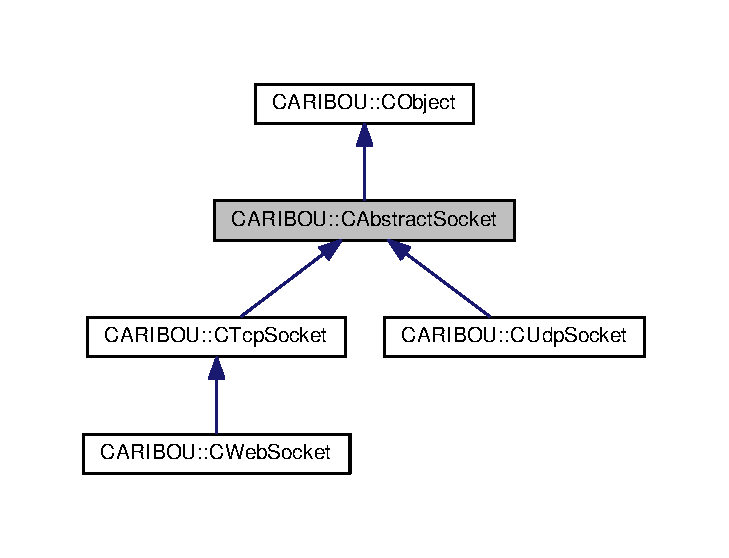
\includegraphics[width=349pt]{class_c_a_r_i_b_o_u_1_1_c_abstract_socket__inherit__graph}
\end{center}
\end{figure}


Collaboration diagram for C\-A\-R\-I\-B\-O\-U\-:\-:C\-Abstract\-Socket\-:\nopagebreak
\begin{figure}[H]
\begin{center}
\leavevmode
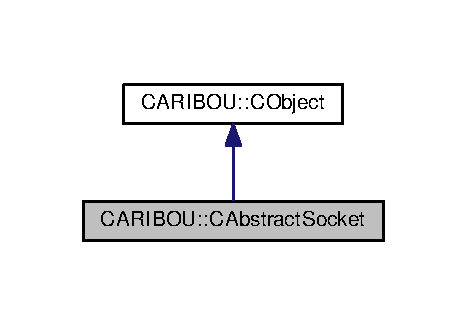
\includegraphics[width=224pt]{class_c_a_r_i_b_o_u_1_1_c_abstract_socket__coll__graph}
\end{center}
\end{figure}
\subsection*{Public Member Functions}
\begin{DoxyCompactItemize}
\item 
{\bf C\-Abstract\-Socket} ()
\item 
{\bf C\-Abstract\-Socket} (int {\bf socket})
\item 
{\bf C\-Abstract\-Socket} (int domain, int type, int protocol)
\item 
{\bf C\-Abstract\-Socket} (const {\bf C\-Abstract\-Socket} \&other)
\item 
virtual {\bf $\sim$\-C\-Abstract\-Socket} ()
\item 
bool {\bf is\-Open} ()
\item 
bool {\bf is\-Valid} ()
\item 
void {\bf abort} ()
\item 
void {\bf close} ()
\begin{DoxyCompactList}\small\item\em Close the socket. \end{DoxyCompactList}\item 
void {\bf shutdown} (int mode=S\-H\-U\-T\-\_\-\-R\-D)
\begin{DoxyCompactList}\small\item\em Sutdown the socket. \end{DoxyCompactList}\item 
bool {\bf set\-Blocking} (bool {\bf blocking})
\begin{DoxyCompactList}\small\item\em Set or clear socket blocking mode Return true on success. \end{DoxyCompactList}\item 
bool {\bf blocking} ()
\begin{DoxyCompactList}\small\item\em Return current blocking mode. \end{DoxyCompactList}\item 
int {\bf bytes\-Available} ()
\begin{DoxyCompactList}\small\item\em Return the number of bytes available in the receive queue. \end{DoxyCompactList}\item 
int {\bf recv} (char $\ast$buf, int len, int flags=0)
\begin{DoxyCompactList}\small\item\em Received bytes. \end{DoxyCompactList}\item 
int {\bf recv} ({\bf C\-A\-R\-I\-B\-O\-U\-::\-C\-Byte\-Array} \&buf, int len, int flags=0)
\begin{DoxyCompactList}\small\item\em Received bytes. \end{DoxyCompactList}\item 
virtual int {\bf send} (char $\ast$buf, int len=-\/1, int flags=0)
\begin{DoxyCompactList}\small\item\em Sends bytes. \end{DoxyCompactList}\item 
virtual int {\bf send} ({\bf C\-A\-R\-I\-B\-O\-U\-::\-C\-Byte\-Array} \&buf, int flags=0)
\begin{DoxyCompactList}\small\item\em Sends bytes. \end{DoxyCompactList}\item 
int {\bf read} (char $\ast$buf, int len)
\begin{DoxyCompactList}\small\item\em Reads bytes received. \end{DoxyCompactList}\item 
int {\bf read} ({\bf C\-A\-R\-I\-B\-O\-U\-::\-C\-Byte\-Array} \&buf, int len)
\begin{DoxyCompactList}\small\item\em Reads bytes received. \end{DoxyCompactList}\item 
int {\bf read} ({\bf C\-A\-R\-I\-B\-O\-U\-::\-C\-Byte\-Array} \&buf, int len, int {\bf timeout})
\begin{DoxyCompactList}\small\item\em Reads bytes received. \end{DoxyCompactList}\item 
int {\bf peek} (char $\ast$buf, int len)
\begin{DoxyCompactList}\small\item\em Peeks bytes received. \end{DoxyCompactList}\item 
int {\bf write} (char $\ast$buf, int len)
\begin{DoxyCompactList}\small\item\em Sends data on a connection. \end{DoxyCompactList}\item 
int {\bf write} ({\bf C\-Byte\-Array} \&buf)
\begin{DoxyCompactList}\small\item\em Sends data on a connection. \end{DoxyCompactList}\item 
uint32\-\_\-t {\bf local\-Address} ()
\begin{DoxyCompactList}\small\item\em Returns the host address of the local socket if available; otherwise returns N\-U\-L\-L. \end{DoxyCompactList}\item 
{\bf C\-String} {\bf local\-Address\-String} ()
\begin{DoxyCompactList}\small\item\em Return the host address of the local socket as a string. \end{DoxyCompactList}\item 
uint16\-\_\-t {\bf local\-Port} ()
\begin{DoxyCompactList}\small\item\em Returns the host port number (in native byte order) of the local socket if available; otherwise returns 0. \end{DoxyCompactList}\item 
uint32\-\_\-t {\bf peer\-Address} ()
\begin{DoxyCompactList}\small\item\em Returns the address of the connected peer if the socket is in Connected\-State; otherwise returns Null. \end{DoxyCompactList}\item 
{\bf C\-String} {\bf peer\-Address\-String} ()
\begin{DoxyCompactList}\small\item\em Return the host address of the local socket as a string. \end{DoxyCompactList}\item 
uint16\-\_\-t {\bf peer\-Port} ()
\begin{DoxyCompactList}\small\item\em Returns the port of the connected peer if the socket is in Connected\-State; otherwise returns 0. \end{DoxyCompactList}\item 
int {\bf accept} ()
\item 
int {\bf listen} (int backlog)
\item 
int {\bf bind} ({\bf C\-A\-R\-I\-B\-O\-U\-::\-C\-String} host=\char`\"{}\char`\"{}, uint16\-\_\-t port=0)
\item 
int {\bf connect\-To\-Host} ({\bf C\-A\-R\-I\-B\-O\-U\-::\-C\-String} host, uint16\-\_\-t port, uint16\-\_\-t host\-Port=0)
\item 
void {\bf disconnect\-From\-Host} ()
\item 
int {\bf set\-Socket} (int {\bf socket})
\item 
int {\bf socket} ()
\item 
bool {\bf timeout} ()
\item 
void {\bf reset\-Timeout} ()
\item 
void {\bf set\-Timeout\-Value} (uint32\-\_\-t {\bf timeout\-Value})
\item 
uint32\-\_\-t {\bf timeout\-Value} ()
\item 
{\bf C\-Abstract\-Socket} \& {\bf operator=} (const {\bf C\-Abstract\-Socket} \&other)
\item 
bool {\bf operator==} ({\bf C\-Abstract\-Socket} \&other)
\end{DoxyCompactItemize}
\subsection*{Protected Member Functions}
\begin{DoxyCompactItemize}
\item 
{\bf C\-String} {\bf address\-String} (uint32\-\_\-t ip)
\begin{DoxyCompactList}\small\item\em Return the host address of the local socket as a string. \end{DoxyCompactList}\end{DoxyCompactItemize}
\subsection*{Protected Attributes}
\begin{DoxyCompactItemize}
\item 
int {\bf m\-Socket}
\item 
uint32\-\_\-t {\bf m\-Timeout\-Mark}
\item 
uint32\-\_\-t {\bf m\-Timeout\-Value}
\item 
uint32\-\_\-t {\bf m\-Peer\-Address}
\item 
uint16\-\_\-t {\bf m\-Peer\-Port}
\end{DoxyCompactItemize}
\subsection*{Additional Inherited Members}


\subsection{Detailed Description}
The \doxyref{C\-Abstract\-Socket}{p.}{class_c_a_r_i_b_o_u_1_1_c_abstract_socket} class provides the base functionality common to all socket types. 

\doxyref{C\-Abstract\-Socket}{p.}{class_c_a_r_i_b_o_u_1_1_c_abstract_socket} is the base class for \doxyref{C\-Tcp\-Socket}{p.}{class_c_a_r_i_b_o_u_1_1_c_tcp_socket} and \doxyref{C\-Udp\-Socket}{p.}{class_c_a_r_i_b_o_u_1_1_c_udp_socket} and contains all common functionality of these two classes. 

Definition at line 34 of file cabstractsocket.\-h.



\subsection{Constructor \& Destructor Documentation}
\index{C\-A\-R\-I\-B\-O\-U\-::\-C\-Abstract\-Socket@{C\-A\-R\-I\-B\-O\-U\-::\-C\-Abstract\-Socket}!C\-Abstract\-Socket@{C\-Abstract\-Socket}}
\index{C\-Abstract\-Socket@{C\-Abstract\-Socket}!CARIBOU::CAbstractSocket@{C\-A\-R\-I\-B\-O\-U\-::\-C\-Abstract\-Socket}}
\subsubsection[{C\-Abstract\-Socket}]{\setlength{\rightskip}{0pt plus 5cm}C\-A\-R\-I\-B\-O\-U\-::\-C\-Abstract\-Socket\-::\-C\-Abstract\-Socket (
\begin{DoxyParamCaption}
{}
\end{DoxyParamCaption}
)}\label{class_c_a_r_i_b_o_u_1_1_c_abstract_socket_adf510bb1c53d556eaf3c859b041c3fa6}


Definition at line 23 of file cabstractsocket.\-cpp.

\index{C\-A\-R\-I\-B\-O\-U\-::\-C\-Abstract\-Socket@{C\-A\-R\-I\-B\-O\-U\-::\-C\-Abstract\-Socket}!C\-Abstract\-Socket@{C\-Abstract\-Socket}}
\index{C\-Abstract\-Socket@{C\-Abstract\-Socket}!CARIBOU::CAbstractSocket@{C\-A\-R\-I\-B\-O\-U\-::\-C\-Abstract\-Socket}}
\subsubsection[{C\-Abstract\-Socket}]{\setlength{\rightskip}{0pt plus 5cm}C\-A\-R\-I\-B\-O\-U\-::\-C\-Abstract\-Socket\-::\-C\-Abstract\-Socket (
\begin{DoxyParamCaption}
\item[{int}]{socket}
\end{DoxyParamCaption}
)}\label{class_c_a_r_i_b_o_u_1_1_c_abstract_socket_adf911e4168e3aeb74ba103c3fe7a2e32}


Definition at line 32 of file cabstractsocket.\-cpp.

\index{C\-A\-R\-I\-B\-O\-U\-::\-C\-Abstract\-Socket@{C\-A\-R\-I\-B\-O\-U\-::\-C\-Abstract\-Socket}!C\-Abstract\-Socket@{C\-Abstract\-Socket}}
\index{C\-Abstract\-Socket@{C\-Abstract\-Socket}!CARIBOU::CAbstractSocket@{C\-A\-R\-I\-B\-O\-U\-::\-C\-Abstract\-Socket}}
\subsubsection[{C\-Abstract\-Socket}]{\setlength{\rightskip}{0pt plus 5cm}C\-A\-R\-I\-B\-O\-U\-::\-C\-Abstract\-Socket\-::\-C\-Abstract\-Socket (
\begin{DoxyParamCaption}
\item[{int}]{domain, }
\item[{int}]{type, }
\item[{int}]{protocol}
\end{DoxyParamCaption}
)}\label{class_c_a_r_i_b_o_u_1_1_c_abstract_socket_a79ea048bb727d94b09bf4124a3dcece6}


Definition at line 41 of file cabstractsocket.\-cpp.

\index{C\-A\-R\-I\-B\-O\-U\-::\-C\-Abstract\-Socket@{C\-A\-R\-I\-B\-O\-U\-::\-C\-Abstract\-Socket}!C\-Abstract\-Socket@{C\-Abstract\-Socket}}
\index{C\-Abstract\-Socket@{C\-Abstract\-Socket}!CARIBOU::CAbstractSocket@{C\-A\-R\-I\-B\-O\-U\-::\-C\-Abstract\-Socket}}
\subsubsection[{C\-Abstract\-Socket}]{\setlength{\rightskip}{0pt plus 5cm}C\-A\-R\-I\-B\-O\-U\-::\-C\-Abstract\-Socket\-::\-C\-Abstract\-Socket (
\begin{DoxyParamCaption}
\item[{const {\bf C\-Abstract\-Socket} \&}]{other}
\end{DoxyParamCaption}
)}\label{class_c_a_r_i_b_o_u_1_1_c_abstract_socket_a697b4dfd446ec58fdb77daedeadf5a14}


Definition at line 50 of file cabstractsocket.\-cpp.

\index{C\-A\-R\-I\-B\-O\-U\-::\-C\-Abstract\-Socket@{C\-A\-R\-I\-B\-O\-U\-::\-C\-Abstract\-Socket}!$\sim$\-C\-Abstract\-Socket@{$\sim$\-C\-Abstract\-Socket}}
\index{$\sim$\-C\-Abstract\-Socket@{$\sim$\-C\-Abstract\-Socket}!CARIBOU::CAbstractSocket@{C\-A\-R\-I\-B\-O\-U\-::\-C\-Abstract\-Socket}}
\subsubsection[{$\sim$\-C\-Abstract\-Socket}]{\setlength{\rightskip}{0pt plus 5cm}C\-A\-R\-I\-B\-O\-U\-::\-C\-Abstract\-Socket\-::$\sim$\-C\-Abstract\-Socket (
\begin{DoxyParamCaption}
{}
\end{DoxyParamCaption}
)\hspace{0.3cm}{\ttfamily [virtual]}}\label{class_c_a_r_i_b_o_u_1_1_c_abstract_socket_a04a040e196125acd1b8f2d64fd20a31b}


Definition at line 59 of file cabstractsocket.\-cpp.



\subsection{Member Function Documentation}
\index{C\-A\-R\-I\-B\-O\-U\-::\-C\-Abstract\-Socket@{C\-A\-R\-I\-B\-O\-U\-::\-C\-Abstract\-Socket}!abort@{abort}}
\index{abort@{abort}!CARIBOU::CAbstractSocket@{C\-A\-R\-I\-B\-O\-U\-::\-C\-Abstract\-Socket}}
\subsubsection[{abort}]{\setlength{\rightskip}{0pt plus 5cm}void C\-A\-R\-I\-B\-O\-U\-::\-C\-Abstract\-Socket\-::abort (
\begin{DoxyParamCaption}
{}
\end{DoxyParamCaption}
)}\label{class_c_a_r_i_b_o_u_1_1_c_abstract_socket_af96e821ff611395a1649fa7326d2bc56}


Definition at line 119 of file cabstractsocket.\-cpp.

\index{C\-A\-R\-I\-B\-O\-U\-::\-C\-Abstract\-Socket@{C\-A\-R\-I\-B\-O\-U\-::\-C\-Abstract\-Socket}!accept@{accept}}
\index{accept@{accept}!CARIBOU::CAbstractSocket@{C\-A\-R\-I\-B\-O\-U\-::\-C\-Abstract\-Socket}}
\subsubsection[{accept}]{\setlength{\rightskip}{0pt plus 5cm}int C\-A\-R\-I\-B\-O\-U\-::\-C\-Abstract\-Socket\-::accept (
\begin{DoxyParamCaption}
{}
\end{DoxyParamCaption}
)}\label{class_c_a_r_i_b_o_u_1_1_c_abstract_socket_adf03cc15fca3d28fe54bc6daa0f0d269}


Definition at line 483 of file cabstractsocket.\-cpp.

\index{C\-A\-R\-I\-B\-O\-U\-::\-C\-Abstract\-Socket@{C\-A\-R\-I\-B\-O\-U\-::\-C\-Abstract\-Socket}!address\-String@{address\-String}}
\index{address\-String@{address\-String}!CARIBOU::CAbstractSocket@{C\-A\-R\-I\-B\-O\-U\-::\-C\-Abstract\-Socket}}
\subsubsection[{address\-String}]{\setlength{\rightskip}{0pt plus 5cm}{\bf C\-A\-R\-I\-B\-O\-U\-::\-C\-String} C\-A\-R\-I\-B\-O\-U\-::\-C\-Abstract\-Socket\-::address\-String (
\begin{DoxyParamCaption}
\item[{uint32\-\_\-t}]{ip}
\end{DoxyParamCaption}
)\hspace{0.3cm}{\ttfamily [protected]}}\label{class_c_a_r_i_b_o_u_1_1_c_abstract_socket_a46044f945c5fa3cdcc4ae7619a0fbf61}


Return the host address of the local socket as a string. 



Definition at line 360 of file cabstractsocket.\-cpp.

\index{C\-A\-R\-I\-B\-O\-U\-::\-C\-Abstract\-Socket@{C\-A\-R\-I\-B\-O\-U\-::\-C\-Abstract\-Socket}!bind@{bind}}
\index{bind@{bind}!CARIBOU::CAbstractSocket@{C\-A\-R\-I\-B\-O\-U\-::\-C\-Abstract\-Socket}}
\subsubsection[{bind}]{\setlength{\rightskip}{0pt plus 5cm}int C\-A\-R\-I\-B\-O\-U\-::\-C\-Abstract\-Socket\-::bind (
\begin{DoxyParamCaption}
\item[{{\bf C\-A\-R\-I\-B\-O\-U\-::\-C\-String}}]{host = {\ttfamily \char`\"{}\char`\"{}}, }
\item[{uint16\-\_\-t}]{port = {\ttfamily 0}}
\end{DoxyParamCaption}
)}\label{class_c_a_r_i_b_o_u_1_1_c_abstract_socket_ac7dbbcc8466fe8703315f3f6d4cb2dc6}


Definition at line 495 of file cabstractsocket.\-cpp.

\index{C\-A\-R\-I\-B\-O\-U\-::\-C\-Abstract\-Socket@{C\-A\-R\-I\-B\-O\-U\-::\-C\-Abstract\-Socket}!blocking@{blocking}}
\index{blocking@{blocking}!CARIBOU::CAbstractSocket@{C\-A\-R\-I\-B\-O\-U\-::\-C\-Abstract\-Socket}}
\subsubsection[{blocking}]{\setlength{\rightskip}{0pt plus 5cm}bool C\-A\-R\-I\-B\-O\-U\-::\-C\-Abstract\-Socket\-::blocking (
\begin{DoxyParamCaption}
{}
\end{DoxyParamCaption}
)}\label{class_c_a_r_i_b_o_u_1_1_c_abstract_socket_af9cbe5cceabc513c956b654ce7cc4bd6}


Return current blocking mode. 



Definition at line 475 of file cabstractsocket.\-cpp.

\index{C\-A\-R\-I\-B\-O\-U\-::\-C\-Abstract\-Socket@{C\-A\-R\-I\-B\-O\-U\-::\-C\-Abstract\-Socket}!bytes\-Available@{bytes\-Available}}
\index{bytes\-Available@{bytes\-Available}!CARIBOU::CAbstractSocket@{C\-A\-R\-I\-B\-O\-U\-::\-C\-Abstract\-Socket}}
\subsubsection[{bytes\-Available}]{\setlength{\rightskip}{0pt plus 5cm}int C\-A\-R\-I\-B\-O\-U\-::\-C\-Abstract\-Socket\-::bytes\-Available (
\begin{DoxyParamCaption}
{}
\end{DoxyParamCaption}
)}\label{class_c_a_r_i_b_o_u_1_1_c_abstract_socket_a5e2aa48733b6c548d76437f71078f2f1}


Return the number of bytes available in the receive queue. 



Definition at line 153 of file cabstractsocket.\-cpp.

\index{C\-A\-R\-I\-B\-O\-U\-::\-C\-Abstract\-Socket@{C\-A\-R\-I\-B\-O\-U\-::\-C\-Abstract\-Socket}!close@{close}}
\index{close@{close}!CARIBOU::CAbstractSocket@{C\-A\-R\-I\-B\-O\-U\-::\-C\-Abstract\-Socket}}
\subsubsection[{close}]{\setlength{\rightskip}{0pt plus 5cm}void C\-A\-R\-I\-B\-O\-U\-::\-C\-Abstract\-Socket\-::close (
\begin{DoxyParamCaption}
{}
\end{DoxyParamCaption}
)}\label{class_c_a_r_i_b_o_u_1_1_c_abstract_socket_a30db92703e334c4103ad0e25de4f12c5}


Close the socket. 



Definition at line 129 of file cabstractsocket.\-cpp.

\index{C\-A\-R\-I\-B\-O\-U\-::\-C\-Abstract\-Socket@{C\-A\-R\-I\-B\-O\-U\-::\-C\-Abstract\-Socket}!connect\-To\-Host@{connect\-To\-Host}}
\index{connect\-To\-Host@{connect\-To\-Host}!CARIBOU::CAbstractSocket@{C\-A\-R\-I\-B\-O\-U\-::\-C\-Abstract\-Socket}}
\subsubsection[{connect\-To\-Host}]{\setlength{\rightskip}{0pt plus 5cm}int C\-A\-R\-I\-B\-O\-U\-::\-C\-Abstract\-Socket\-::connect\-To\-Host (
\begin{DoxyParamCaption}
\item[{{\bf C\-A\-R\-I\-B\-O\-U\-::\-C\-String}}]{host, }
\item[{uint16\-\_\-t}]{port, }
\item[{uint16\-\_\-t}]{host\-Port = {\ttfamily 0}}
\end{DoxyParamCaption}
)}\label{class_c_a_r_i_b_o_u_1_1_c_abstract_socket_abf3d344b822f35c5303033e4bbd5f241}


Definition at line 520 of file cabstractsocket.\-cpp.

\index{C\-A\-R\-I\-B\-O\-U\-::\-C\-Abstract\-Socket@{C\-A\-R\-I\-B\-O\-U\-::\-C\-Abstract\-Socket}!disconnect\-From\-Host@{disconnect\-From\-Host}}
\index{disconnect\-From\-Host@{disconnect\-From\-Host}!CARIBOU::CAbstractSocket@{C\-A\-R\-I\-B\-O\-U\-::\-C\-Abstract\-Socket}}
\subsubsection[{disconnect\-From\-Host}]{\setlength{\rightskip}{0pt plus 5cm}void C\-A\-R\-I\-B\-O\-U\-::\-C\-Abstract\-Socket\-::disconnect\-From\-Host (
\begin{DoxyParamCaption}
{}
\end{DoxyParamCaption}
)}\label{class_c_a_r_i_b_o_u_1_1_c_abstract_socket_a85d6968bdc15657134b854e4152b1e7f}


Definition at line 542 of file cabstractsocket.\-cpp.

\index{C\-A\-R\-I\-B\-O\-U\-::\-C\-Abstract\-Socket@{C\-A\-R\-I\-B\-O\-U\-::\-C\-Abstract\-Socket}!is\-Open@{is\-Open}}
\index{is\-Open@{is\-Open}!CARIBOU::CAbstractSocket@{C\-A\-R\-I\-B\-O\-U\-::\-C\-Abstract\-Socket}}
\subsubsection[{is\-Open}]{\setlength{\rightskip}{0pt plus 5cm}bool C\-A\-R\-I\-B\-O\-U\-::\-C\-Abstract\-Socket\-::is\-Open (
\begin{DoxyParamCaption}
{}
\end{DoxyParamCaption}
)}\label{class_c_a_r_i_b_o_u_1_1_c_abstract_socket_abe65a016b0c7dbae8309c05d3d2eb75d}

\begin{DoxyItemize}
\item 0, the remote host closed the connection
\item $>$0, data was received,
\item $<$0, there has been an error. To find out which error, you have to look Return the number of bytes available in the receive queue. 
\end{DoxyItemize}

Definition at line 98 of file cabstractsocket.\-cpp.

\index{C\-A\-R\-I\-B\-O\-U\-::\-C\-Abstract\-Socket@{C\-A\-R\-I\-B\-O\-U\-::\-C\-Abstract\-Socket}!is\-Valid@{is\-Valid}}
\index{is\-Valid@{is\-Valid}!CARIBOU::CAbstractSocket@{C\-A\-R\-I\-B\-O\-U\-::\-C\-Abstract\-Socket}}
\subsubsection[{is\-Valid}]{\setlength{\rightskip}{0pt plus 5cm}bool C\-A\-R\-I\-B\-O\-U\-::\-C\-Abstract\-Socket\-::is\-Valid (
\begin{DoxyParamCaption}
{}
\end{DoxyParamCaption}
)}\label{class_c_a_r_i_b_o_u_1_1_c_abstract_socket_a01dc9f0934c7b33f7770c872fcf3939c}


Definition at line 114 of file cabstractsocket.\-cpp.

\index{C\-A\-R\-I\-B\-O\-U\-::\-C\-Abstract\-Socket@{C\-A\-R\-I\-B\-O\-U\-::\-C\-Abstract\-Socket}!listen@{listen}}
\index{listen@{listen}!CARIBOU::CAbstractSocket@{C\-A\-R\-I\-B\-O\-U\-::\-C\-Abstract\-Socket}}
\subsubsection[{listen}]{\setlength{\rightskip}{0pt plus 5cm}int C\-A\-R\-I\-B\-O\-U\-::\-C\-Abstract\-Socket\-::listen (
\begin{DoxyParamCaption}
\item[{int}]{backlog}
\end{DoxyParamCaption}
)}\label{class_c_a_r_i_b_o_u_1_1_c_abstract_socket_aef46677db9742c5ffa5996b326a41eb4}


Definition at line 489 of file cabstractsocket.\-cpp.

\index{C\-A\-R\-I\-B\-O\-U\-::\-C\-Abstract\-Socket@{C\-A\-R\-I\-B\-O\-U\-::\-C\-Abstract\-Socket}!local\-Address@{local\-Address}}
\index{local\-Address@{local\-Address}!CARIBOU::CAbstractSocket@{C\-A\-R\-I\-B\-O\-U\-::\-C\-Abstract\-Socket}}
\subsubsection[{local\-Address}]{\setlength{\rightskip}{0pt plus 5cm}uint32\-\_\-t C\-A\-R\-I\-B\-O\-U\-::\-C\-Abstract\-Socket\-::local\-Address (
\begin{DoxyParamCaption}
{}
\end{DoxyParamCaption}
)}\label{class_c_a_r_i_b_o_u_1_1_c_abstract_socket_a47459e1b3dd9e26085dac1b858023933}


Returns the host address of the local socket if available; otherwise returns N\-U\-L\-L. 

This is normally the main I\-P address of the host, but can be (127.\-0.\-0.\-1) for connections to the local host. 

Definition at line 380 of file cabstractsocket.\-cpp.

\index{C\-A\-R\-I\-B\-O\-U\-::\-C\-Abstract\-Socket@{C\-A\-R\-I\-B\-O\-U\-::\-C\-Abstract\-Socket}!local\-Address\-String@{local\-Address\-String}}
\index{local\-Address\-String@{local\-Address\-String}!CARIBOU::CAbstractSocket@{C\-A\-R\-I\-B\-O\-U\-::\-C\-Abstract\-Socket}}
\subsubsection[{local\-Address\-String}]{\setlength{\rightskip}{0pt plus 5cm}{\bf C\-A\-R\-I\-B\-O\-U\-::\-C\-String} C\-A\-R\-I\-B\-O\-U\-::\-C\-Abstract\-Socket\-::local\-Address\-String (
\begin{DoxyParamCaption}
{}
\end{DoxyParamCaption}
)}\label{class_c_a_r_i_b_o_u_1_1_c_abstract_socket_aadc2b9e706e2197be8e8d7d8b991661b}


Return the host address of the local socket as a string. 



Definition at line 367 of file cabstractsocket.\-cpp.

\index{C\-A\-R\-I\-B\-O\-U\-::\-C\-Abstract\-Socket@{C\-A\-R\-I\-B\-O\-U\-::\-C\-Abstract\-Socket}!local\-Port@{local\-Port}}
\index{local\-Port@{local\-Port}!CARIBOU::CAbstractSocket@{C\-A\-R\-I\-B\-O\-U\-::\-C\-Abstract\-Socket}}
\subsubsection[{local\-Port}]{\setlength{\rightskip}{0pt plus 5cm}uint16\-\_\-t C\-A\-R\-I\-B\-O\-U\-::\-C\-Abstract\-Socket\-::local\-Port (
\begin{DoxyParamCaption}
{}
\end{DoxyParamCaption}
)}\label{class_c_a_r_i_b_o_u_1_1_c_abstract_socket_abc6d696d81f453abd5d3a97f49817cd3}


Returns the host port number (in native byte order) of the local socket if available; otherwise returns 0. 



Definition at line 400 of file cabstractsocket.\-cpp.

\index{C\-A\-R\-I\-B\-O\-U\-::\-C\-Abstract\-Socket@{C\-A\-R\-I\-B\-O\-U\-::\-C\-Abstract\-Socket}!operator=@{operator=}}
\index{operator=@{operator=}!CARIBOU::CAbstractSocket@{C\-A\-R\-I\-B\-O\-U\-::\-C\-Abstract\-Socket}}
\subsubsection[{operator=}]{\setlength{\rightskip}{0pt plus 5cm}{\bf C\-Abstract\-Socket} \& C\-A\-R\-I\-B\-O\-U\-::\-C\-Abstract\-Socket\-::operator= (
\begin{DoxyParamCaption}
\item[{const {\bf C\-Abstract\-Socket} \&}]{other}
\end{DoxyParamCaption}
)}\label{class_c_a_r_i_b_o_u_1_1_c_abstract_socket_ad07ef7e000add9bc0c5a2493ac172de9}


Definition at line 64 of file cabstractsocket.\-cpp.

\index{C\-A\-R\-I\-B\-O\-U\-::\-C\-Abstract\-Socket@{C\-A\-R\-I\-B\-O\-U\-::\-C\-Abstract\-Socket}!operator==@{operator==}}
\index{operator==@{operator==}!CARIBOU::CAbstractSocket@{C\-A\-R\-I\-B\-O\-U\-::\-C\-Abstract\-Socket}}
\subsubsection[{operator==}]{\setlength{\rightskip}{0pt plus 5cm}bool C\-A\-R\-I\-B\-O\-U\-::\-C\-Abstract\-Socket\-::operator== (
\begin{DoxyParamCaption}
\item[{{\bf C\-Abstract\-Socket} \&}]{other}
\end{DoxyParamCaption}
)}\label{class_c_a_r_i_b_o_u_1_1_c_abstract_socket_aaeeb5bbee7bdc9cca4b3e420de7ec253}


Definition at line 72 of file cabstractsocket.\-cpp.

\index{C\-A\-R\-I\-B\-O\-U\-::\-C\-Abstract\-Socket@{C\-A\-R\-I\-B\-O\-U\-::\-C\-Abstract\-Socket}!peek@{peek}}
\index{peek@{peek}!CARIBOU::CAbstractSocket@{C\-A\-R\-I\-B\-O\-U\-::\-C\-Abstract\-Socket}}
\subsubsection[{peek}]{\setlength{\rightskip}{0pt plus 5cm}int C\-A\-R\-I\-B\-O\-U\-::\-C\-Abstract\-Socket\-::peek (
\begin{DoxyParamCaption}
\item[{char $\ast$}]{buf, }
\item[{int}]{len}
\end{DoxyParamCaption}
)}\label{class_c_a_r_i_b_o_u_1_1_c_abstract_socket_accb76a62bd0ef8fd1f1d0ccb0bbddab0}


Peeks bytes received. 

In the B\-S\-D socket A\-P\-I, the \doxyref{read()}{p.}{class_c_a_r_i_b_o_u_1_1_c_abstract_socket_a0b96a7c40304b4a1e925df4664395805} function are used on a connected socket to receive data. If the received message is larger than the supplied memory area, the excess data is silently discarded. 

Definition at line 252 of file cabstractsocket.\-cpp.

\index{C\-A\-R\-I\-B\-O\-U\-::\-C\-Abstract\-Socket@{C\-A\-R\-I\-B\-O\-U\-::\-C\-Abstract\-Socket}!peer\-Address@{peer\-Address}}
\index{peer\-Address@{peer\-Address}!CARIBOU::CAbstractSocket@{C\-A\-R\-I\-B\-O\-U\-::\-C\-Abstract\-Socket}}
\subsubsection[{peer\-Address}]{\setlength{\rightskip}{0pt plus 5cm}uint32\-\_\-t C\-A\-R\-I\-B\-O\-U\-::\-C\-Abstract\-Socket\-::peer\-Address (
\begin{DoxyParamCaption}
{}
\end{DoxyParamCaption}
)}\label{class_c_a_r_i_b_o_u_1_1_c_abstract_socket_adc3eb133ca07aaa3bef89faefb3e6acb}


Returns the address of the connected peer if the socket is in Connected\-State; otherwise returns Null. 



Definition at line 416 of file cabstractsocket.\-cpp.

\index{C\-A\-R\-I\-B\-O\-U\-::\-C\-Abstract\-Socket@{C\-A\-R\-I\-B\-O\-U\-::\-C\-Abstract\-Socket}!peer\-Address\-String@{peer\-Address\-String}}
\index{peer\-Address\-String@{peer\-Address\-String}!CARIBOU::CAbstractSocket@{C\-A\-R\-I\-B\-O\-U\-::\-C\-Abstract\-Socket}}
\subsubsection[{peer\-Address\-String}]{\setlength{\rightskip}{0pt plus 5cm}{\bf C\-A\-R\-I\-B\-O\-U\-::\-C\-String} C\-A\-R\-I\-B\-O\-U\-::\-C\-Abstract\-Socket\-::peer\-Address\-String (
\begin{DoxyParamCaption}
{}
\end{DoxyParamCaption}
)}\label{class_c_a_r_i_b_o_u_1_1_c_abstract_socket_a090421e50c95eb614e03935ca84d029d}


Return the host address of the local socket as a string. 



Definition at line 373 of file cabstractsocket.\-cpp.

\index{C\-A\-R\-I\-B\-O\-U\-::\-C\-Abstract\-Socket@{C\-A\-R\-I\-B\-O\-U\-::\-C\-Abstract\-Socket}!peer\-Port@{peer\-Port}}
\index{peer\-Port@{peer\-Port}!CARIBOU::CAbstractSocket@{C\-A\-R\-I\-B\-O\-U\-::\-C\-Abstract\-Socket}}
\subsubsection[{peer\-Port}]{\setlength{\rightskip}{0pt plus 5cm}uint16\-\_\-t C\-A\-R\-I\-B\-O\-U\-::\-C\-Abstract\-Socket\-::peer\-Port (
\begin{DoxyParamCaption}
{}
\end{DoxyParamCaption}
)}\label{class_c_a_r_i_b_o_u_1_1_c_abstract_socket_a4d4055533858919fff38896c4a035d8a}


Returns the port of the connected peer if the socket is in Connected\-State; otherwise returns 0. 



Definition at line 439 of file cabstractsocket.\-cpp.

\index{C\-A\-R\-I\-B\-O\-U\-::\-C\-Abstract\-Socket@{C\-A\-R\-I\-B\-O\-U\-::\-C\-Abstract\-Socket}!read@{read}}
\index{read@{read}!CARIBOU::CAbstractSocket@{C\-A\-R\-I\-B\-O\-U\-::\-C\-Abstract\-Socket}}
\subsubsection[{read}]{\setlength{\rightskip}{0pt plus 5cm}int C\-A\-R\-I\-B\-O\-U\-::\-C\-Abstract\-Socket\-::read (
\begin{DoxyParamCaption}
\item[{char $\ast$}]{buf, }
\item[{int}]{len}
\end{DoxyParamCaption}
)}\label{class_c_a_r_i_b_o_u_1_1_c_abstract_socket_a0b96a7c40304b4a1e925df4664395805}


Reads bytes received. 

In the B\-S\-D socket A\-P\-I, the \doxyref{read()}{p.}{class_c_a_r_i_b_o_u_1_1_c_abstract_socket_a0b96a7c40304b4a1e925df4664395805} function are used on a connected socket to receive data. If the received message is larger than the supplied memory area, the excess data is silently discarded. 

Definition at line 263 of file cabstractsocket.\-cpp.

\index{C\-A\-R\-I\-B\-O\-U\-::\-C\-Abstract\-Socket@{C\-A\-R\-I\-B\-O\-U\-::\-C\-Abstract\-Socket}!read@{read}}
\index{read@{read}!CARIBOU::CAbstractSocket@{C\-A\-R\-I\-B\-O\-U\-::\-C\-Abstract\-Socket}}
\subsubsection[{read}]{\setlength{\rightskip}{0pt plus 5cm}int C\-A\-R\-I\-B\-O\-U\-::\-C\-Abstract\-Socket\-::read (
\begin{DoxyParamCaption}
\item[{{\bf C\-A\-R\-I\-B\-O\-U\-::\-C\-Byte\-Array} \&}]{buf, }
\item[{int}]{len}
\end{DoxyParamCaption}
)}\label{class_c_a_r_i_b_o_u_1_1_c_abstract_socket_ae574c5fa812a2c27eacd8df369c80ba8}


Reads bytes received. 

In the B\-S\-D socket A\-P\-I, the \doxyref{read()}{p.}{class_c_a_r_i_b_o_u_1_1_c_abstract_socket_a0b96a7c40304b4a1e925df4664395805} function are used on a connected socket to receive data. If the received message is larger than the supplied memory area, the excess data is silently discarded. 

Definition at line 272 of file cabstractsocket.\-cpp.

\index{C\-A\-R\-I\-B\-O\-U\-::\-C\-Abstract\-Socket@{C\-A\-R\-I\-B\-O\-U\-::\-C\-Abstract\-Socket}!read@{read}}
\index{read@{read}!CARIBOU::CAbstractSocket@{C\-A\-R\-I\-B\-O\-U\-::\-C\-Abstract\-Socket}}
\subsubsection[{read}]{\setlength{\rightskip}{0pt plus 5cm}int C\-A\-R\-I\-B\-O\-U\-::\-C\-Abstract\-Socket\-::read (
\begin{DoxyParamCaption}
\item[{{\bf C\-A\-R\-I\-B\-O\-U\-::\-C\-Byte\-Array} \&}]{buf, }
\item[{int}]{len, }
\item[{int}]{timeout}
\end{DoxyParamCaption}
)}\label{class_c_a_r_i_b_o_u_1_1_c_abstract_socket_ad1c7c5d74d6c2a2566018aec9b9197b4}


Reads bytes received. 

In the B\-S\-D socket A\-P\-I, the \doxyref{read()}{p.}{class_c_a_r_i_b_o_u_1_1_c_abstract_socket_a0b96a7c40304b4a1e925df4664395805} function are used on a connected socket to receive data. If the received message is larger than the supplied memory area, the excess data is silently discarded. 
\begin{DoxyParams}{Parameters}
{\em timeout} & The time to wait for recieved data in miliseconds. \\
\hline
\end{DoxyParams}


Definition at line 288 of file cabstractsocket.\-cpp.

\index{C\-A\-R\-I\-B\-O\-U\-::\-C\-Abstract\-Socket@{C\-A\-R\-I\-B\-O\-U\-::\-C\-Abstract\-Socket}!recv@{recv}}
\index{recv@{recv}!CARIBOU::CAbstractSocket@{C\-A\-R\-I\-B\-O\-U\-::\-C\-Abstract\-Socket}}
\subsubsection[{recv}]{\setlength{\rightskip}{0pt plus 5cm}int C\-A\-R\-I\-B\-O\-U\-::\-C\-Abstract\-Socket\-::recv (
\begin{DoxyParamCaption}
\item[{char $\ast$}]{buf, }
\item[{int}]{len, }
\item[{int}]{flags = {\ttfamily 0}}
\end{DoxyParamCaption}
)}\label{class_c_a_r_i_b_o_u_1_1_c_abstract_socket_aa349b0ec128d2b87abd5c6a2df00dbc5}


Received bytes. 

In the B\-S\-D socket A\-P\-I, the \doxyref{recv()}{p.}{class_c_a_r_i_b_o_u_1_1_c_abstract_socket_aa349b0ec128d2b87abd5c6a2df00dbc5} calls are used on a connected socket to receive data. A number of flags can be passed by the call to \doxyref{recv()}{p.}{class_c_a_r_i_b_o_u_1_1_c_abstract_socket_aa349b0ec128d2b87abd5c6a2df00dbc5}. If the received message is larger than the supplied memory area, the excess data is silently discarded. 
\begin{DoxyParams}{Parameters}
{\em buf} & Memory buffer to store received data. \\
\hline
{\em len} & Length to data to receiving. \\
\hline
{\em flags} & User shall use one of followings\-: M\-S\-G\-\_\-\-P\-E\-E\-K -\/ Peeks at an incoming message M\-S\-G\-\_\-\-D\-O\-N\-T\-W\-A\-I\-T -\/ Nonblocking i/o for this operation only M\-S\-G\-\_\-\-M\-O\-R\-E -\/ Wait for more than one message \\
\hline
\end{DoxyParams}


Definition at line 178 of file cabstractsocket.\-cpp.

\index{C\-A\-R\-I\-B\-O\-U\-::\-C\-Abstract\-Socket@{C\-A\-R\-I\-B\-O\-U\-::\-C\-Abstract\-Socket}!recv@{recv}}
\index{recv@{recv}!CARIBOU::CAbstractSocket@{C\-A\-R\-I\-B\-O\-U\-::\-C\-Abstract\-Socket}}
\subsubsection[{recv}]{\setlength{\rightskip}{0pt plus 5cm}int C\-A\-R\-I\-B\-O\-U\-::\-C\-Abstract\-Socket\-::recv (
\begin{DoxyParamCaption}
\item[{{\bf C\-A\-R\-I\-B\-O\-U\-::\-C\-Byte\-Array} \&}]{buf, }
\item[{int}]{len, }
\item[{int}]{flags = {\ttfamily 0}}
\end{DoxyParamCaption}
)}\label{class_c_a_r_i_b_o_u_1_1_c_abstract_socket_a8f9ecc1e22a04b4bebbfc6b695c2a49c}


Received bytes. 

In the B\-S\-D socket A\-P\-I, the \doxyref{recv()}{p.}{class_c_a_r_i_b_o_u_1_1_c_abstract_socket_aa349b0ec128d2b87abd5c6a2df00dbc5} calls are used on a connected socket to receive data. A number of flags can be passed by the call to \doxyref{recv()}{p.}{class_c_a_r_i_b_o_u_1_1_c_abstract_socket_aa349b0ec128d2b87abd5c6a2df00dbc5}. If the received message is larger than the supplied memory area, the excess data is silently discarded. 
\begin{DoxyParams}{Parameters}
{\em buf} & Memory buffer to store received data. \\
\hline
{\em len} & Length to data to receiving. \\
\hline
{\em flags} & User shall use one of followings\-: M\-S\-G\-\_\-\-P\-E\-E\-K -\/ Peeks at an incoming message M\-S\-G\-\_\-\-D\-O\-N\-T\-W\-A\-I\-T -\/ Nonblocking i/o for this operation only M\-S\-G\-\_\-\-M\-O\-R\-E -\/ Wait for more than one message \\
\hline
\end{DoxyParams}


Definition at line 194 of file cabstractsocket.\-cpp.

\index{C\-A\-R\-I\-B\-O\-U\-::\-C\-Abstract\-Socket@{C\-A\-R\-I\-B\-O\-U\-::\-C\-Abstract\-Socket}!reset\-Timeout@{reset\-Timeout}}
\index{reset\-Timeout@{reset\-Timeout}!CARIBOU::CAbstractSocket@{C\-A\-R\-I\-B\-O\-U\-::\-C\-Abstract\-Socket}}
\subsubsection[{reset\-Timeout}]{\setlength{\rightskip}{0pt plus 5cm}void C\-A\-R\-I\-B\-O\-U\-::\-C\-Abstract\-Socket\-::reset\-Timeout (
\begin{DoxyParamCaption}
{}
\end{DoxyParamCaption}
)}\label{class_c_a_r_i_b_o_u_1_1_c_abstract_socket_a8d49d3e1e95ddce033d955b9ca4f4b87}


Definition at line 82 of file cabstractsocket.\-cpp.

\index{C\-A\-R\-I\-B\-O\-U\-::\-C\-Abstract\-Socket@{C\-A\-R\-I\-B\-O\-U\-::\-C\-Abstract\-Socket}!send@{send}}
\index{send@{send}!CARIBOU::CAbstractSocket@{C\-A\-R\-I\-B\-O\-U\-::\-C\-Abstract\-Socket}}
\subsubsection[{send}]{\setlength{\rightskip}{0pt plus 5cm}int C\-A\-R\-I\-B\-O\-U\-::\-C\-Abstract\-Socket\-::send (
\begin{DoxyParamCaption}
\item[{char $\ast$}]{buf, }
\item[{int}]{len = {\ttfamily -\/1}, }
\item[{int}]{flags = {\ttfamily 0}}
\end{DoxyParamCaption}
)\hspace{0.3cm}{\ttfamily [virtual]}}\label{class_c_a_r_i_b_o_u_1_1_c_abstract_socket_a77a751bf9d01c60f17c0f5d8299dba69}


Sends bytes. 

This function is used in T\-C\-P connection for sending data. Before a call to lwip\-\_\-send() the receiver of the data must have been set up using lwip\-\_\-connect(). 
\begin{DoxyParams}{Parameters}
{\em buf} & Data buffer to send. \\
\hline
{\em len} & Size of the data; (-\/1) means a zero-\/terminated string \\
\hline
{\em flag} & User can use this flags\-: 0x00 -\/ No Flags M\-S\-G\-\_\-\-P\-E\-E\-K -\/ Peeks at an incoming message M\-S\-G\-\_\-\-D\-O\-N\-T\-W\-A\-I\-T -\/ Nonblocking i/o for this operation only M\-S\-G\-\_\-\-M\-O\-R\-E -\/ Sender will send more \\
\hline
\end{DoxyParams}
\begin{DoxyReturn}{Returns}
Number of bytes sent, -\/1 = Failure 
\end{DoxyReturn}


Reimplemented in {\bf C\-A\-R\-I\-B\-O\-U\-::\-C\-Udp\-Socket} \doxyref{}{p.}{class_c_a_r_i_b_o_u_1_1_c_udp_socket_ab0fe3c7f7ecd38f6092c8f64cd1c9afa}.



Definition at line 217 of file cabstractsocket.\-cpp.

\index{C\-A\-R\-I\-B\-O\-U\-::\-C\-Abstract\-Socket@{C\-A\-R\-I\-B\-O\-U\-::\-C\-Abstract\-Socket}!send@{send}}
\index{send@{send}!CARIBOU::CAbstractSocket@{C\-A\-R\-I\-B\-O\-U\-::\-C\-Abstract\-Socket}}
\subsubsection[{send}]{\setlength{\rightskip}{0pt plus 5cm}int C\-A\-R\-I\-B\-O\-U\-::\-C\-Abstract\-Socket\-::send (
\begin{DoxyParamCaption}
\item[{{\bf C\-A\-R\-I\-B\-O\-U\-::\-C\-Byte\-Array} \&}]{buf, }
\item[{int}]{flags = {\ttfamily 0}}
\end{DoxyParamCaption}
)\hspace{0.3cm}{\ttfamily [virtual]}}\label{class_c_a_r_i_b_o_u_1_1_c_abstract_socket_a1cfbf919281241f7ad2d2be86de2a8e4}


Sends bytes. 

This function is used in T\-C\-P connection for sending data. Before a call to lwip\-\_\-send() the receiver of the data must have been set up using lwip\-\_\-connect(). 
\begin{DoxyParams}{Parameters}
{\em buf} & Data buffer to send. \\
\hline
{\em len} & Size of the data. \\
\hline
{\em flag} & User can use this flags\-: 0x00 -\/ No Flags M\-S\-G\-\_\-\-P\-E\-E\-K -\/ Peeks at an incoming message M\-S\-G\-\_\-\-D\-O\-N\-T\-W\-A\-I\-T -\/ Nonblocking i/o for this operation only M\-S\-G\-\_\-\-M\-O\-R\-E -\/ Sender will send more \\
\hline
\end{DoxyParams}
\begin{DoxyReturn}{Returns}
Number of bytes sent, -\/1 = Failure 
\end{DoxyReturn}


Reimplemented in {\bf C\-A\-R\-I\-B\-O\-U\-::\-C\-Udp\-Socket} \doxyref{}{p.}{class_c_a_r_i_b_o_u_1_1_c_udp_socket_a8e15ad0d1e0eaa1a91f2e8a5ce5ad94d}.



Definition at line 240 of file cabstractsocket.\-cpp.

\index{C\-A\-R\-I\-B\-O\-U\-::\-C\-Abstract\-Socket@{C\-A\-R\-I\-B\-O\-U\-::\-C\-Abstract\-Socket}!set\-Blocking@{set\-Blocking}}
\index{set\-Blocking@{set\-Blocking}!CARIBOU::CAbstractSocket@{C\-A\-R\-I\-B\-O\-U\-::\-C\-Abstract\-Socket}}
\subsubsection[{set\-Blocking}]{\setlength{\rightskip}{0pt plus 5cm}bool C\-A\-R\-I\-B\-O\-U\-::\-C\-Abstract\-Socket\-::set\-Blocking (
\begin{DoxyParamCaption}
\item[{bool}]{blocking}
\end{DoxyParamCaption}
)}\label{class_c_a_r_i_b_o_u_1_1_c_abstract_socket_a5fa404ac162a60fdc00e5178a7ea4b29}


Set or clear socket blocking mode Return true on success. 



Definition at line 463 of file cabstractsocket.\-cpp.

\index{C\-A\-R\-I\-B\-O\-U\-::\-C\-Abstract\-Socket@{C\-A\-R\-I\-B\-O\-U\-::\-C\-Abstract\-Socket}!set\-Socket@{set\-Socket}}
\index{set\-Socket@{set\-Socket}!CARIBOU::CAbstractSocket@{C\-A\-R\-I\-B\-O\-U\-::\-C\-Abstract\-Socket}}
\subsubsection[{set\-Socket}]{\setlength{\rightskip}{0pt plus 5cm}int C\-A\-R\-I\-B\-O\-U\-::\-C\-Abstract\-Socket\-::set\-Socket (
\begin{DoxyParamCaption}
\item[{int}]{socket}
\end{DoxyParamCaption}
)\hspace{0.3cm}{\ttfamily [inline]}}\label{class_c_a_r_i_b_o_u_1_1_c_abstract_socket_a1b6ca0145cd5a03c7c27d63e586355ea}


Definition at line 83 of file cabstractsocket.\-h.

\index{C\-A\-R\-I\-B\-O\-U\-::\-C\-Abstract\-Socket@{C\-A\-R\-I\-B\-O\-U\-::\-C\-Abstract\-Socket}!set\-Timeout\-Value@{set\-Timeout\-Value}}
\index{set\-Timeout\-Value@{set\-Timeout\-Value}!CARIBOU::CAbstractSocket@{C\-A\-R\-I\-B\-O\-U\-::\-C\-Abstract\-Socket}}
\subsubsection[{set\-Timeout\-Value}]{\setlength{\rightskip}{0pt plus 5cm}void C\-A\-R\-I\-B\-O\-U\-::\-C\-Abstract\-Socket\-::set\-Timeout\-Value (
\begin{DoxyParamCaption}
\item[{uint32\-\_\-t}]{timeout\-Value}
\end{DoxyParamCaption}
)}\label{class_c_a_r_i_b_o_u_1_1_c_abstract_socket_a3d714c0f6a512abf4fe5e97177131b43}


Definition at line 87 of file cabstractsocket.\-cpp.

\index{C\-A\-R\-I\-B\-O\-U\-::\-C\-Abstract\-Socket@{C\-A\-R\-I\-B\-O\-U\-::\-C\-Abstract\-Socket}!shutdown@{shutdown}}
\index{shutdown@{shutdown}!CARIBOU::CAbstractSocket@{C\-A\-R\-I\-B\-O\-U\-::\-C\-Abstract\-Socket}}
\subsubsection[{shutdown}]{\setlength{\rightskip}{0pt plus 5cm}void C\-A\-R\-I\-B\-O\-U\-::\-C\-Abstract\-Socket\-::shutdown (
\begin{DoxyParamCaption}
\item[{int}]{mode = {\ttfamily SHUT\-\_\-RD}}
\end{DoxyParamCaption}
)}\label{class_c_a_r_i_b_o_u_1_1_c_abstract_socket_a173e77105a1e51b581ff102f3c1bc733}


Sutdown the socket. 



Definition at line 141 of file cabstractsocket.\-cpp.

\index{C\-A\-R\-I\-B\-O\-U\-::\-C\-Abstract\-Socket@{C\-A\-R\-I\-B\-O\-U\-::\-C\-Abstract\-Socket}!socket@{socket}}
\index{socket@{socket}!CARIBOU::CAbstractSocket@{C\-A\-R\-I\-B\-O\-U\-::\-C\-Abstract\-Socket}}
\subsubsection[{socket}]{\setlength{\rightskip}{0pt plus 5cm}int C\-A\-R\-I\-B\-O\-U\-::\-C\-Abstract\-Socket\-::socket (
\begin{DoxyParamCaption}
{}
\end{DoxyParamCaption}
)\hspace{0.3cm}{\ttfamily [inline]}}\label{class_c_a_r_i_b_o_u_1_1_c_abstract_socket_a39973ad7c3e834596ae448c4768086e1}


Definition at line 84 of file cabstractsocket.\-h.

\index{C\-A\-R\-I\-B\-O\-U\-::\-C\-Abstract\-Socket@{C\-A\-R\-I\-B\-O\-U\-::\-C\-Abstract\-Socket}!timeout@{timeout}}
\index{timeout@{timeout}!CARIBOU::CAbstractSocket@{C\-A\-R\-I\-B\-O\-U\-::\-C\-Abstract\-Socket}}
\subsubsection[{timeout}]{\setlength{\rightskip}{0pt plus 5cm}bool C\-A\-R\-I\-B\-O\-U\-::\-C\-Abstract\-Socket\-::timeout (
\begin{DoxyParamCaption}
{}
\end{DoxyParamCaption}
)}\label{class_c_a_r_i_b_o_u_1_1_c_abstract_socket_accf8af63ddf05c58ce1b0cabc3659c59}


Definition at line 77 of file cabstractsocket.\-cpp.

\index{C\-A\-R\-I\-B\-O\-U\-::\-C\-Abstract\-Socket@{C\-A\-R\-I\-B\-O\-U\-::\-C\-Abstract\-Socket}!timeout\-Value@{timeout\-Value}}
\index{timeout\-Value@{timeout\-Value}!CARIBOU::CAbstractSocket@{C\-A\-R\-I\-B\-O\-U\-::\-C\-Abstract\-Socket}}
\subsubsection[{timeout\-Value}]{\setlength{\rightskip}{0pt plus 5cm}uint32\-\_\-t C\-A\-R\-I\-B\-O\-U\-::\-C\-Abstract\-Socket\-::timeout\-Value (
\begin{DoxyParamCaption}
{}
\end{DoxyParamCaption}
)}\label{class_c_a_r_i_b_o_u_1_1_c_abstract_socket_a4f725ee32ee4004fd3a386df363357f2}


Definition at line 92 of file cabstractsocket.\-cpp.

\index{C\-A\-R\-I\-B\-O\-U\-::\-C\-Abstract\-Socket@{C\-A\-R\-I\-B\-O\-U\-::\-C\-Abstract\-Socket}!write@{write}}
\index{write@{write}!CARIBOU::CAbstractSocket@{C\-A\-R\-I\-B\-O\-U\-::\-C\-Abstract\-Socket}}
\subsubsection[{write}]{\setlength{\rightskip}{0pt plus 5cm}int C\-A\-R\-I\-B\-O\-U\-::\-C\-Abstract\-Socket\-::write (
\begin{DoxyParamCaption}
\item[{char $\ast$}]{buf, }
\item[{int}]{len}
\end{DoxyParamCaption}
)}\label{class_c_a_r_i_b_o_u_1_1_c_abstract_socket_a7c8dac542a56700f57db41e19cd242c5}


Sends data on a connection. 

This function is used in T\-C\-P connection for sending data. Before a call to \doxyref{write()}{p.}{class_c_a_r_i_b_o_u_1_1_c_abstract_socket_a7c8dac542a56700f57db41e19cd242c5} the receiver of the data must have been set up using connect(). This function is equvalent to the \doxyref{send()}{p.}{class_c_a_r_i_b_o_u_1_1_c_abstract_socket_a77a751bf9d01c60f17c0f5d8299dba69} function. 

Definition at line 337 of file cabstractsocket.\-cpp.

\index{C\-A\-R\-I\-B\-O\-U\-::\-C\-Abstract\-Socket@{C\-A\-R\-I\-B\-O\-U\-::\-C\-Abstract\-Socket}!write@{write}}
\index{write@{write}!CARIBOU::CAbstractSocket@{C\-A\-R\-I\-B\-O\-U\-::\-C\-Abstract\-Socket}}
\subsubsection[{write}]{\setlength{\rightskip}{0pt plus 5cm}int C\-A\-R\-I\-B\-O\-U\-::\-C\-Abstract\-Socket\-::write (
\begin{DoxyParamCaption}
\item[{{\bf C\-Byte\-Array} \&}]{buf}
\end{DoxyParamCaption}
)}\label{class_c_a_r_i_b_o_u_1_1_c_abstract_socket_acdf63ac4bab14d1a9abfd779229903a0}


Sends data on a connection. 

This function is used in T\-C\-P connection for sending data. Before a call to \doxyref{write()}{p.}{class_c_a_r_i_b_o_u_1_1_c_abstract_socket_a7c8dac542a56700f57db41e19cd242c5} the receiver of the data must have been set up using connect(). This function is equvalent to the \doxyref{send()}{p.}{class_c_a_r_i_b_o_u_1_1_c_abstract_socket_a77a751bf9d01c60f17c0f5d8299dba69} function. 

Definition at line 350 of file cabstractsocket.\-cpp.



\subsection{Member Data Documentation}
\index{C\-A\-R\-I\-B\-O\-U\-::\-C\-Abstract\-Socket@{C\-A\-R\-I\-B\-O\-U\-::\-C\-Abstract\-Socket}!m\-Peer\-Address@{m\-Peer\-Address}}
\index{m\-Peer\-Address@{m\-Peer\-Address}!CARIBOU::CAbstractSocket@{C\-A\-R\-I\-B\-O\-U\-::\-C\-Abstract\-Socket}}
\subsubsection[{m\-Peer\-Address}]{\setlength{\rightskip}{0pt plus 5cm}uint32\-\_\-t C\-A\-R\-I\-B\-O\-U\-::\-C\-Abstract\-Socket\-::m\-Peer\-Address\hspace{0.3cm}{\ttfamily [protected]}}\label{class_c_a_r_i_b_o_u_1_1_c_abstract_socket_ae68c89abeaa7efbf5e6ea863e8b544fd}


Definition at line 100 of file cabstractsocket.\-h.

\index{C\-A\-R\-I\-B\-O\-U\-::\-C\-Abstract\-Socket@{C\-A\-R\-I\-B\-O\-U\-::\-C\-Abstract\-Socket}!m\-Peer\-Port@{m\-Peer\-Port}}
\index{m\-Peer\-Port@{m\-Peer\-Port}!CARIBOU::CAbstractSocket@{C\-A\-R\-I\-B\-O\-U\-::\-C\-Abstract\-Socket}}
\subsubsection[{m\-Peer\-Port}]{\setlength{\rightskip}{0pt plus 5cm}uint16\-\_\-t C\-A\-R\-I\-B\-O\-U\-::\-C\-Abstract\-Socket\-::m\-Peer\-Port\hspace{0.3cm}{\ttfamily [protected]}}\label{class_c_a_r_i_b_o_u_1_1_c_abstract_socket_ae5604f528c22caa58c01948f6649c731}


Definition at line 101 of file cabstractsocket.\-h.

\index{C\-A\-R\-I\-B\-O\-U\-::\-C\-Abstract\-Socket@{C\-A\-R\-I\-B\-O\-U\-::\-C\-Abstract\-Socket}!m\-Socket@{m\-Socket}}
\index{m\-Socket@{m\-Socket}!CARIBOU::CAbstractSocket@{C\-A\-R\-I\-B\-O\-U\-::\-C\-Abstract\-Socket}}
\subsubsection[{m\-Socket}]{\setlength{\rightskip}{0pt plus 5cm}int C\-A\-R\-I\-B\-O\-U\-::\-C\-Abstract\-Socket\-::m\-Socket\hspace{0.3cm}{\ttfamily [protected]}}\label{class_c_a_r_i_b_o_u_1_1_c_abstract_socket_ae352aa1ae212553fd13400437b4bd386}


Definition at line 97 of file cabstractsocket.\-h.

\index{C\-A\-R\-I\-B\-O\-U\-::\-C\-Abstract\-Socket@{C\-A\-R\-I\-B\-O\-U\-::\-C\-Abstract\-Socket}!m\-Timeout\-Mark@{m\-Timeout\-Mark}}
\index{m\-Timeout\-Mark@{m\-Timeout\-Mark}!CARIBOU::CAbstractSocket@{C\-A\-R\-I\-B\-O\-U\-::\-C\-Abstract\-Socket}}
\subsubsection[{m\-Timeout\-Mark}]{\setlength{\rightskip}{0pt plus 5cm}uint32\-\_\-t C\-A\-R\-I\-B\-O\-U\-::\-C\-Abstract\-Socket\-::m\-Timeout\-Mark\hspace{0.3cm}{\ttfamily [protected]}}\label{class_c_a_r_i_b_o_u_1_1_c_abstract_socket_a757cee10572d8a4117b14ff03c8711d6}


Definition at line 98 of file cabstractsocket.\-h.

\index{C\-A\-R\-I\-B\-O\-U\-::\-C\-Abstract\-Socket@{C\-A\-R\-I\-B\-O\-U\-::\-C\-Abstract\-Socket}!m\-Timeout\-Value@{m\-Timeout\-Value}}
\index{m\-Timeout\-Value@{m\-Timeout\-Value}!CARIBOU::CAbstractSocket@{C\-A\-R\-I\-B\-O\-U\-::\-C\-Abstract\-Socket}}
\subsubsection[{m\-Timeout\-Value}]{\setlength{\rightskip}{0pt plus 5cm}uint32\-\_\-t C\-A\-R\-I\-B\-O\-U\-::\-C\-Abstract\-Socket\-::m\-Timeout\-Value\hspace{0.3cm}{\ttfamily [protected]}}\label{class_c_a_r_i_b_o_u_1_1_c_abstract_socket_af2ba77f9a08be3f15193a9d96a95e77b}


Definition at line 99 of file cabstractsocket.\-h.



The documentation for this class was generated from the following files\-:\begin{DoxyCompactItemize}
\item 
include/caribou++/{\bf cabstractsocket.\-h}\item 
src/{\bf cabstractsocket.\-cpp}\end{DoxyCompactItemize}

\section{C\-A\-R\-I\-B\-O\-U\-:\-:C\-Base64 Class Reference}
\label{class_c_a_r_i_b_o_u_1_1_c_base64}\index{C\-A\-R\-I\-B\-O\-U\-::\-C\-Base64@{C\-A\-R\-I\-B\-O\-U\-::\-C\-Base64}}


{\ttfamily \#include $<$cbase64.\-h$>$}

\subsection*{Public Member Functions}
\begin{DoxyCompactItemize}
\item 
{\bf C\-Base64} ()
\item 
{\bf C\-Base64} (const {\bf C\-A\-R\-I\-B\-O\-U\-::\-C\-String} in)
\item 
{\bf $\sim$\-C\-Base64} ()
\item 
{\bf C\-A\-R\-I\-B\-O\-U\-::\-C\-Byte\-Array} {\bf encode} ({\bf C\-A\-R\-I\-B\-O\-U\-::\-C\-Byte\-Array} in)
\item 
{\bf C\-A\-R\-I\-B\-O\-U\-::\-C\-Byte\-Array} {\bf decode} ({\bf C\-A\-R\-I\-B\-O\-U\-::\-C\-Byte\-Array} in)
\end{DoxyCompactItemize}


\subsection{Detailed Description}


Definition at line 25 of file cbase64.\-h.



\subsection{Constructor \& Destructor Documentation}
\index{C\-A\-R\-I\-B\-O\-U\-::\-C\-Base64@{C\-A\-R\-I\-B\-O\-U\-::\-C\-Base64}!C\-Base64@{C\-Base64}}
\index{C\-Base64@{C\-Base64}!CARIBOU::CBase64@{C\-A\-R\-I\-B\-O\-U\-::\-C\-Base64}}
\subsubsection[{C\-Base64}]{\setlength{\rightskip}{0pt plus 5cm}C\-A\-R\-I\-B\-O\-U\-::\-C\-Base64\-::\-C\-Base64 (
\begin{DoxyParamCaption}
{}
\end{DoxyParamCaption}
)}\label{class_c_a_r_i_b_o_u_1_1_c_base64_af08848b15801054091ae81fa6fabc819}


Definition at line 69 of file cbase64.\-cpp.

\index{C\-A\-R\-I\-B\-O\-U\-::\-C\-Base64@{C\-A\-R\-I\-B\-O\-U\-::\-C\-Base64}!C\-Base64@{C\-Base64}}
\index{C\-Base64@{C\-Base64}!CARIBOU::CBase64@{C\-A\-R\-I\-B\-O\-U\-::\-C\-Base64}}
\subsubsection[{C\-Base64}]{\setlength{\rightskip}{0pt plus 5cm}C\-A\-R\-I\-B\-O\-U\-::\-C\-Base64\-::\-C\-Base64 (
\begin{DoxyParamCaption}
\item[{const {\bf C\-A\-R\-I\-B\-O\-U\-::\-C\-String}}]{in}
\end{DoxyParamCaption}
)}\label{class_c_a_r_i_b_o_u_1_1_c_base64_a44ca0ffa9b2b3e5736cad2ade2158e76}


Definition at line 73 of file cbase64.\-cpp.

\index{C\-A\-R\-I\-B\-O\-U\-::\-C\-Base64@{C\-A\-R\-I\-B\-O\-U\-::\-C\-Base64}!$\sim$\-C\-Base64@{$\sim$\-C\-Base64}}
\index{$\sim$\-C\-Base64@{$\sim$\-C\-Base64}!CARIBOU::CBase64@{C\-A\-R\-I\-B\-O\-U\-::\-C\-Base64}}
\subsubsection[{$\sim$\-C\-Base64}]{\setlength{\rightskip}{0pt plus 5cm}C\-A\-R\-I\-B\-O\-U\-::\-C\-Base64\-::$\sim$\-C\-Base64 (
\begin{DoxyParamCaption}
{}
\end{DoxyParamCaption}
)}\label{class_c_a_r_i_b_o_u_1_1_c_base64_a0373578618d9e99fde4364b22c99f788}


Definition at line 77 of file cbase64.\-cpp.



\subsection{Member Function Documentation}
\index{C\-A\-R\-I\-B\-O\-U\-::\-C\-Base64@{C\-A\-R\-I\-B\-O\-U\-::\-C\-Base64}!decode@{decode}}
\index{decode@{decode}!CARIBOU::CBase64@{C\-A\-R\-I\-B\-O\-U\-::\-C\-Base64}}
\subsubsection[{decode}]{\setlength{\rightskip}{0pt plus 5cm}{\bf C\-A\-R\-I\-B\-O\-U\-::\-C\-Byte\-Array} C\-A\-R\-I\-B\-O\-U\-::\-C\-Base64\-::decode (
\begin{DoxyParamCaption}
\item[{{\bf C\-A\-R\-I\-B\-O\-U\-::\-C\-Byte\-Array}}]{in}
\end{DoxyParamCaption}
)}\label{class_c_a_r_i_b_o_u_1_1_c_base64_a6898a45706f57cf3db0177323c32c7d5}


Definition at line 120 of file cbase64.\-cpp.

\index{C\-A\-R\-I\-B\-O\-U\-::\-C\-Base64@{C\-A\-R\-I\-B\-O\-U\-::\-C\-Base64}!encode@{encode}}
\index{encode@{encode}!CARIBOU::CBase64@{C\-A\-R\-I\-B\-O\-U\-::\-C\-Base64}}
\subsubsection[{encode}]{\setlength{\rightskip}{0pt plus 5cm}{\bf C\-A\-R\-I\-B\-O\-U\-::\-C\-Byte\-Array} C\-A\-R\-I\-B\-O\-U\-::\-C\-Base64\-::encode (
\begin{DoxyParamCaption}
\item[{{\bf C\-A\-R\-I\-B\-O\-U\-::\-C\-Byte\-Array}}]{in}
\end{DoxyParamCaption}
)}\label{class_c_a_r_i_b_o_u_1_1_c_base64_af6ff8c7b6f93d721c185d6bd9fd038ba}


Definition at line 81 of file cbase64.\-cpp.



The documentation for this class was generated from the following files\-:\begin{DoxyCompactItemize}
\item 
include/caribou++/{\bf cbase64.\-h}\item 
src/{\bf cbase64.\-cpp}\end{DoxyCompactItemize}

\section{C\-A\-R\-I\-B\-O\-U\-:\-:C\-Bitmap Class Reference}
\label{class_c_a_r_i_b_o_u_1_1_c_bitmap}\index{C\-A\-R\-I\-B\-O\-U\-::\-C\-Bitmap@{C\-A\-R\-I\-B\-O\-U\-::\-C\-Bitmap}}


Defines a generic bitmap storage class.  




{\ttfamily \#include $<$cbitmap.\-h$>$}



Inheritance diagram for C\-A\-R\-I\-B\-O\-U\-:\-:C\-Bitmap\-:\nopagebreak
\begin{figure}[H]
\begin{center}
\leavevmode
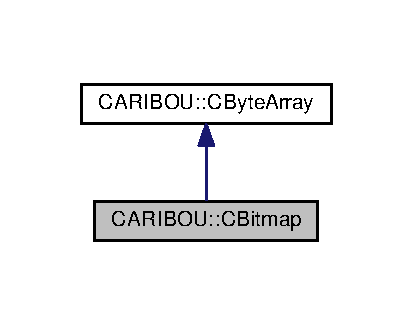
\includegraphics[width=198pt]{class_c_a_r_i_b_o_u_1_1_c_bitmap__inherit__graph}
\end{center}
\end{figure}


Collaboration diagram for C\-A\-R\-I\-B\-O\-U\-:\-:C\-Bitmap\-:\nopagebreak
\begin{figure}[H]
\begin{center}
\leavevmode
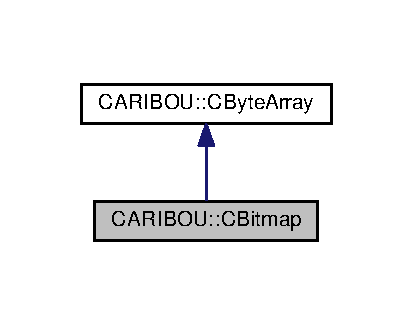
\includegraphics[width=198pt]{class_c_a_r_i_b_o_u_1_1_c_bitmap__coll__graph}
\end{center}
\end{figure}
\subsection*{Public Member Functions}
\begin{DoxyCompactItemize}
\item 
{\bf C\-Bitmap} ()
\item 
{\bf C\-Bitmap} ({\bf C\-Size} {\bf size})
\item 
{\bf C\-Bitmap} (int {\bf width}, int {\bf height})
\item 
{\bf C\-Bitmap} (int {\bf width}, int {\bf height}, const uint8\-\_\-t $\ast${\bf data}, bool big\-Endian=false)
\item 
{\bf C\-Bitmap} (const {\bf C\-Bitmap} \&other)
\item 
virtual {\bf $\sim$\-C\-Bitmap} ()
\item 
void {\bf set\-Bits} (int {\bf width}, int {\bf height}, const uint8\-\_\-t $\ast${\bf data}, bool big\-Endian=true)
\item 
virtual void {\bf clear} ()
\item 
void {\bf resize} ({\bf C\-Size} {\bf size})
\item 
void {\bf resize} (int {\bf width}, int {\bf height})
\begin{DoxyCompactList}\small\item\em Resize the bitmap buffer. \end{DoxyCompactList}\item 
{\bf C\-Size} {\bf dimensions} ()
\item 
int {\bf width} ()
\item 
int {\bf height} ()
\item 
uint8\-\_\-t {\bf bit} (int x, int y)
\item 
void {\bf set\-Bit} (int x, int y, uint8\-\_\-t {\bf bit})
\item 
int {\bf left\-Margin} ()
\begin{DoxyCompactList}\small\item\em Calculate the number of inactive columns of bits between the left edge and the first column containing an active bit. \end{DoxyCompactList}\item 
int {\bf right\-Margin} ()
\begin{DoxyCompactList}\small\item\em Calculate the number of inactive columns of bits between the left edge and the first column containing an active bit. \end{DoxyCompactList}\item 
int {\bf top\-Margin} ()
\begin{DoxyCompactList}\small\item\em Calculate the number of inactive columns of bits between the left edge and the first column containing an active bit. \end{DoxyCompactList}\item 
int {\bf bottom\-Margin} ()
\begin{DoxyCompactList}\small\item\em Calculate the number of inactive columns of bits between the left edge and the first column containing an active bit. \end{DoxyCompactList}\item 
{\bf C\-Bitmap} {\bf trimmed\-Left} (int margin)
\begin{DoxyCompactList}\small\item\em Make a copy of the bitmap with the left edge trimmed. \end{DoxyCompactList}\item 
{\bf C\-Bitmap} {\bf trimmed\-Right} (int margin)
\begin{DoxyCompactList}\small\item\em Make a copy of the bitmap with the right edge trimmed. \end{DoxyCompactList}\item 
{\bf C\-Bitmap} {\bf trimmed\-Top} (int margin)
\begin{DoxyCompactList}\small\item\em Make a copy of the bitmap with the top edge trimmed. \end{DoxyCompactList}\item 
{\bf C\-Bitmap} {\bf trimmed\-Bottom} (int margin)
\begin{DoxyCompactList}\small\item\em Make a copy of the bitmap with the bottom edge trimmed. \end{DoxyCompactList}\end{DoxyCompactItemize}
\subsection*{Additional Inherited Members}


\subsection{Detailed Description}
Defines a generic bitmap storage class. 



Definition at line 27 of file cbitmap.\-h.



\subsection{Constructor \& Destructor Documentation}
\index{C\-A\-R\-I\-B\-O\-U\-::\-C\-Bitmap@{C\-A\-R\-I\-B\-O\-U\-::\-C\-Bitmap}!C\-Bitmap@{C\-Bitmap}}
\index{C\-Bitmap@{C\-Bitmap}!CARIBOU::CBitmap@{C\-A\-R\-I\-B\-O\-U\-::\-C\-Bitmap}}
\subsubsection[{C\-Bitmap}]{\setlength{\rightskip}{0pt plus 5cm}C\-A\-R\-I\-B\-O\-U\-::\-C\-Bitmap\-::\-C\-Bitmap (
\begin{DoxyParamCaption}
{}
\end{DoxyParamCaption}
)}\label{class_c_a_r_i_b_o_u_1_1_c_bitmap_ab8fcc32afe614bab7058a4bcd40a0401}


Definition at line 23 of file cbitmap.\-cpp.

\index{C\-A\-R\-I\-B\-O\-U\-::\-C\-Bitmap@{C\-A\-R\-I\-B\-O\-U\-::\-C\-Bitmap}!C\-Bitmap@{C\-Bitmap}}
\index{C\-Bitmap@{C\-Bitmap}!CARIBOU::CBitmap@{C\-A\-R\-I\-B\-O\-U\-::\-C\-Bitmap}}
\subsubsection[{C\-Bitmap}]{\setlength{\rightskip}{0pt plus 5cm}C\-A\-R\-I\-B\-O\-U\-::\-C\-Bitmap\-::\-C\-Bitmap (
\begin{DoxyParamCaption}
\item[{{\bf C\-Size}}]{size}
\end{DoxyParamCaption}
)}\label{class_c_a_r_i_b_o_u_1_1_c_bitmap_adea5a4c43cca32ab8055b7cc81917c61}


Definition at line 40 of file cbitmap.\-cpp.

\index{C\-A\-R\-I\-B\-O\-U\-::\-C\-Bitmap@{C\-A\-R\-I\-B\-O\-U\-::\-C\-Bitmap}!C\-Bitmap@{C\-Bitmap}}
\index{C\-Bitmap@{C\-Bitmap}!CARIBOU::CBitmap@{C\-A\-R\-I\-B\-O\-U\-::\-C\-Bitmap}}
\subsubsection[{C\-Bitmap}]{\setlength{\rightskip}{0pt plus 5cm}C\-A\-R\-I\-B\-O\-U\-::\-C\-Bitmap\-::\-C\-Bitmap (
\begin{DoxyParamCaption}
\item[{int}]{width, }
\item[{int}]{height}
\end{DoxyParamCaption}
)}\label{class_c_a_r_i_b_o_u_1_1_c_bitmap_a45db767e4c26692bc96440465d0c729a}


Definition at line 34 of file cbitmap.\-cpp.

\index{C\-A\-R\-I\-B\-O\-U\-::\-C\-Bitmap@{C\-A\-R\-I\-B\-O\-U\-::\-C\-Bitmap}!C\-Bitmap@{C\-Bitmap}}
\index{C\-Bitmap@{C\-Bitmap}!CARIBOU::CBitmap@{C\-A\-R\-I\-B\-O\-U\-::\-C\-Bitmap}}
\subsubsection[{C\-Bitmap}]{\setlength{\rightskip}{0pt plus 5cm}C\-A\-R\-I\-B\-O\-U\-::\-C\-Bitmap\-::\-C\-Bitmap (
\begin{DoxyParamCaption}
\item[{int}]{width, }
\item[{int}]{height, }
\item[{const uint8\-\_\-t $\ast$}]{data, }
\item[{bool}]{big\-Endian = {\ttfamily false}}
\end{DoxyParamCaption}
)}\label{class_c_a_r_i_b_o_u_1_1_c_bitmap_a94c6c4c06bd5b860c5db8a1b5253220e}


Definition at line 28 of file cbitmap.\-cpp.

\index{C\-A\-R\-I\-B\-O\-U\-::\-C\-Bitmap@{C\-A\-R\-I\-B\-O\-U\-::\-C\-Bitmap}!C\-Bitmap@{C\-Bitmap}}
\index{C\-Bitmap@{C\-Bitmap}!CARIBOU::CBitmap@{C\-A\-R\-I\-B\-O\-U\-::\-C\-Bitmap}}
\subsubsection[{C\-Bitmap}]{\setlength{\rightskip}{0pt plus 5cm}C\-A\-R\-I\-B\-O\-U\-::\-C\-Bitmap\-::\-C\-Bitmap (
\begin{DoxyParamCaption}
\item[{const {\bf C\-Bitmap} \&}]{other}
\end{DoxyParamCaption}
)}\label{class_c_a_r_i_b_o_u_1_1_c_bitmap_a1c6685d7fd095df32835152dbeefa046}


Definition at line 46 of file cbitmap.\-cpp.

\index{C\-A\-R\-I\-B\-O\-U\-::\-C\-Bitmap@{C\-A\-R\-I\-B\-O\-U\-::\-C\-Bitmap}!$\sim$\-C\-Bitmap@{$\sim$\-C\-Bitmap}}
\index{$\sim$\-C\-Bitmap@{$\sim$\-C\-Bitmap}!CARIBOU::CBitmap@{C\-A\-R\-I\-B\-O\-U\-::\-C\-Bitmap}}
\subsubsection[{$\sim$\-C\-Bitmap}]{\setlength{\rightskip}{0pt plus 5cm}C\-A\-R\-I\-B\-O\-U\-::\-C\-Bitmap\-::$\sim$\-C\-Bitmap (
\begin{DoxyParamCaption}
{}
\end{DoxyParamCaption}
)\hspace{0.3cm}{\ttfamily [virtual]}}\label{class_c_a_r_i_b_o_u_1_1_c_bitmap_a30afa35804c22f930cd339217e278954}


Definition at line 52 of file cbitmap.\-cpp.



\subsection{Member Function Documentation}
\index{C\-A\-R\-I\-B\-O\-U\-::\-C\-Bitmap@{C\-A\-R\-I\-B\-O\-U\-::\-C\-Bitmap}!bit@{bit}}
\index{bit@{bit}!CARIBOU::CBitmap@{C\-A\-R\-I\-B\-O\-U\-::\-C\-Bitmap}}
\subsubsection[{bit}]{\setlength{\rightskip}{0pt plus 5cm}uint8\-\_\-t C\-A\-R\-I\-B\-O\-U\-::\-C\-Bitmap\-::bit (
\begin{DoxyParamCaption}
\item[{int}]{x, }
\item[{int}]{y}
\end{DoxyParamCaption}
)}\label{class_c_a_r_i_b_o_u_1_1_c_bitmap_a8562457af8d4f5b3203963b594ba2a15}
\begin{DoxyReturn}{Returns}
The bit at the x,y position. 
\end{DoxyReturn}


Definition at line 118 of file cbitmap.\-cpp.

\index{C\-A\-R\-I\-B\-O\-U\-::\-C\-Bitmap@{C\-A\-R\-I\-B\-O\-U\-::\-C\-Bitmap}!bottom\-Margin@{bottom\-Margin}}
\index{bottom\-Margin@{bottom\-Margin}!CARIBOU::CBitmap@{C\-A\-R\-I\-B\-O\-U\-::\-C\-Bitmap}}
\subsubsection[{bottom\-Margin}]{\setlength{\rightskip}{0pt plus 5cm}int C\-A\-R\-I\-B\-O\-U\-::\-C\-Bitmap\-::bottom\-Margin (
\begin{DoxyParamCaption}
{}
\end{DoxyParamCaption}
)}\label{class_c_a_r_i_b_o_u_1_1_c_bitmap_a3ddcdf46a9d2362df4323189cc1cf09c}


Calculate the number of inactive columns of bits between the left edge and the first column containing an active bit. 



Definition at line 226 of file cbitmap.\-cpp.

\index{C\-A\-R\-I\-B\-O\-U\-::\-C\-Bitmap@{C\-A\-R\-I\-B\-O\-U\-::\-C\-Bitmap}!clear@{clear}}
\index{clear@{clear}!CARIBOU::CBitmap@{C\-A\-R\-I\-B\-O\-U\-::\-C\-Bitmap}}
\subsubsection[{clear}]{\setlength{\rightskip}{0pt plus 5cm}void C\-A\-R\-I\-B\-O\-U\-::\-C\-Bitmap\-::clear (
\begin{DoxyParamCaption}
{}
\end{DoxyParamCaption}
)\hspace{0.3cm}{\ttfamily [virtual]}}\label{class_c_a_r_i_b_o_u_1_1_c_bitmap_abde5f3ea3c04afd596d13f58f8de06db}


Reimplemented from {\bf C\-A\-R\-I\-B\-O\-U\-::\-C\-Byte\-Array} \doxyref{}{p.}{class_c_a_r_i_b_o_u_1_1_c_byte_array_a21a6406374c2f76a71e3a1f038dbf31a}.



Definition at line 125 of file cbitmap.\-cpp.

\index{C\-A\-R\-I\-B\-O\-U\-::\-C\-Bitmap@{C\-A\-R\-I\-B\-O\-U\-::\-C\-Bitmap}!dimensions@{dimensions}}
\index{dimensions@{dimensions}!CARIBOU::CBitmap@{C\-A\-R\-I\-B\-O\-U\-::\-C\-Bitmap}}
\subsubsection[{dimensions}]{\setlength{\rightskip}{0pt plus 5cm}{\bf C\-Size} C\-A\-R\-I\-B\-O\-U\-::\-C\-Bitmap\-::dimensions (
\begin{DoxyParamCaption}
{}
\end{DoxyParamCaption}
)}\label{class_c_a_r_i_b_o_u_1_1_c_bitmap_a6f65ec9a9115588a487780809bb24e34}


Definition at line 110 of file cbitmap.\-cpp.

\index{C\-A\-R\-I\-B\-O\-U\-::\-C\-Bitmap@{C\-A\-R\-I\-B\-O\-U\-::\-C\-Bitmap}!height@{height}}
\index{height@{height}!CARIBOU::CBitmap@{C\-A\-R\-I\-B\-O\-U\-::\-C\-Bitmap}}
\subsubsection[{height}]{\setlength{\rightskip}{0pt plus 5cm}int C\-A\-R\-I\-B\-O\-U\-::\-C\-Bitmap\-::height (
\begin{DoxyParamCaption}
{}
\end{DoxyParamCaption}
)\hspace{0.3cm}{\ttfamily [inline]}}\label{class_c_a_r_i_b_o_u_1_1_c_bitmap_aa2fc5393c8bb16e6571e98b6b6cbf54e}


Definition at line 44 of file cbitmap.\-h.

\index{C\-A\-R\-I\-B\-O\-U\-::\-C\-Bitmap@{C\-A\-R\-I\-B\-O\-U\-::\-C\-Bitmap}!left\-Margin@{left\-Margin}}
\index{left\-Margin@{left\-Margin}!CARIBOU::CBitmap@{C\-A\-R\-I\-B\-O\-U\-::\-C\-Bitmap}}
\subsubsection[{left\-Margin}]{\setlength{\rightskip}{0pt plus 5cm}int C\-A\-R\-I\-B\-O\-U\-::\-C\-Bitmap\-::left\-Margin (
\begin{DoxyParamCaption}
{}
\end{DoxyParamCaption}
)}\label{class_c_a_r_i_b_o_u_1_1_c_bitmap_a232c623cc4601c7d804af99377daafe5}


Calculate the number of inactive columns of bits between the left edge and the first column containing an active bit. 



Definition at line 166 of file cbitmap.\-cpp.

\index{C\-A\-R\-I\-B\-O\-U\-::\-C\-Bitmap@{C\-A\-R\-I\-B\-O\-U\-::\-C\-Bitmap}!resize@{resize}}
\index{resize@{resize}!CARIBOU::CBitmap@{C\-A\-R\-I\-B\-O\-U\-::\-C\-Bitmap}}
\subsubsection[{resize}]{\setlength{\rightskip}{0pt plus 5cm}void C\-A\-R\-I\-B\-O\-U\-::\-C\-Bitmap\-::resize (
\begin{DoxyParamCaption}
\item[{{\bf C\-Size}}]{size}
\end{DoxyParamCaption}
)\hspace{0.3cm}{\ttfamily [inline]}}\label{class_c_a_r_i_b_o_u_1_1_c_bitmap_aa248fcd53c54c7c58c40b0fcfd1cd4ae}


Definition at line 40 of file cbitmap.\-h.

\index{C\-A\-R\-I\-B\-O\-U\-::\-C\-Bitmap@{C\-A\-R\-I\-B\-O\-U\-::\-C\-Bitmap}!resize@{resize}}
\index{resize@{resize}!CARIBOU::CBitmap@{C\-A\-R\-I\-B\-O\-U\-::\-C\-Bitmap}}
\subsubsection[{resize}]{\setlength{\rightskip}{0pt plus 5cm}void C\-A\-R\-I\-B\-O\-U\-::\-C\-Bitmap\-::resize (
\begin{DoxyParamCaption}
\item[{int}]{width, }
\item[{int}]{height}
\end{DoxyParamCaption}
)}\label{class_c_a_r_i_b_o_u_1_1_c_bitmap_a34958432f952e133818d3ce3de520165}


Resize the bitmap buffer. 



Definition at line 97 of file cbitmap.\-cpp.

\index{C\-A\-R\-I\-B\-O\-U\-::\-C\-Bitmap@{C\-A\-R\-I\-B\-O\-U\-::\-C\-Bitmap}!right\-Margin@{right\-Margin}}
\index{right\-Margin@{right\-Margin}!CARIBOU::CBitmap@{C\-A\-R\-I\-B\-O\-U\-::\-C\-Bitmap}}
\subsubsection[{right\-Margin}]{\setlength{\rightskip}{0pt plus 5cm}int C\-A\-R\-I\-B\-O\-U\-::\-C\-Bitmap\-::right\-Margin (
\begin{DoxyParamCaption}
{}
\end{DoxyParamCaption}
)}\label{class_c_a_r_i_b_o_u_1_1_c_bitmap_a6581bfd877e9a15ff42f09e738faa4f1}


Calculate the number of inactive columns of bits between the left edge and the first column containing an active bit. 



Definition at line 186 of file cbitmap.\-cpp.

\index{C\-A\-R\-I\-B\-O\-U\-::\-C\-Bitmap@{C\-A\-R\-I\-B\-O\-U\-::\-C\-Bitmap}!set\-Bit@{set\-Bit}}
\index{set\-Bit@{set\-Bit}!CARIBOU::CBitmap@{C\-A\-R\-I\-B\-O\-U\-::\-C\-Bitmap}}
\subsubsection[{set\-Bit}]{\setlength{\rightskip}{0pt plus 5cm}void C\-A\-R\-I\-B\-O\-U\-::\-C\-Bitmap\-::set\-Bit (
\begin{DoxyParamCaption}
\item[{int}]{x, }
\item[{int}]{y, }
\item[{uint8\-\_\-t}]{bit}
\end{DoxyParamCaption}
)}\label{class_c_a_r_i_b_o_u_1_1_c_bitmap_a37e34d449690c548eca6afdc2eb5bf11}
\begin{DoxyReturn}{Returns}
The bit at the x,y position. 
\end{DoxyReturn}


Definition at line 134 of file cbitmap.\-cpp.

\index{C\-A\-R\-I\-B\-O\-U\-::\-C\-Bitmap@{C\-A\-R\-I\-B\-O\-U\-::\-C\-Bitmap}!set\-Bits@{set\-Bits}}
\index{set\-Bits@{set\-Bits}!CARIBOU::CBitmap@{C\-A\-R\-I\-B\-O\-U\-::\-C\-Bitmap}}
\subsubsection[{set\-Bits}]{\setlength{\rightskip}{0pt plus 5cm}void C\-A\-R\-I\-B\-O\-U\-::\-C\-Bitmap\-::set\-Bits (
\begin{DoxyParamCaption}
\item[{int}]{width, }
\item[{int}]{height, }
\item[{const uint8\-\_\-t $\ast$}]{data, }
\item[{bool}]{big\-Endian = {\ttfamily true}}
\end{DoxyParamCaption}
)}\label{class_c_a_r_i_b_o_u_1_1_c_bitmap_a9c6540ce8ad29bd4033aeceb8f7d5649}


Definition at line 56 of file cbitmap.\-cpp.

\index{C\-A\-R\-I\-B\-O\-U\-::\-C\-Bitmap@{C\-A\-R\-I\-B\-O\-U\-::\-C\-Bitmap}!top\-Margin@{top\-Margin}}
\index{top\-Margin@{top\-Margin}!CARIBOU::CBitmap@{C\-A\-R\-I\-B\-O\-U\-::\-C\-Bitmap}}
\subsubsection[{top\-Margin}]{\setlength{\rightskip}{0pt plus 5cm}int C\-A\-R\-I\-B\-O\-U\-::\-C\-Bitmap\-::top\-Margin (
\begin{DoxyParamCaption}
{}
\end{DoxyParamCaption}
)}\label{class_c_a_r_i_b_o_u_1_1_c_bitmap_a4abf3ab23d8a994e584b2e2f5823b431}


Calculate the number of inactive columns of bits between the left edge and the first column containing an active bit. 



Definition at line 206 of file cbitmap.\-cpp.

\index{C\-A\-R\-I\-B\-O\-U\-::\-C\-Bitmap@{C\-A\-R\-I\-B\-O\-U\-::\-C\-Bitmap}!trimmed\-Bottom@{trimmed\-Bottom}}
\index{trimmed\-Bottom@{trimmed\-Bottom}!CARIBOU::CBitmap@{C\-A\-R\-I\-B\-O\-U\-::\-C\-Bitmap}}
\subsubsection[{trimmed\-Bottom}]{\setlength{\rightskip}{0pt plus 5cm}{\bf C\-Bitmap} C\-A\-R\-I\-B\-O\-U\-::\-C\-Bitmap\-::trimmed\-Bottom (
\begin{DoxyParamCaption}
\item[{int}]{margin}
\end{DoxyParamCaption}
)}\label{class_c_a_r_i_b_o_u_1_1_c_bitmap_a22c04c48e9b8794edf07fff80eb71cf7}


Make a copy of the bitmap with the bottom edge trimmed. 



Definition at line 305 of file cbitmap.\-cpp.

\index{C\-A\-R\-I\-B\-O\-U\-::\-C\-Bitmap@{C\-A\-R\-I\-B\-O\-U\-::\-C\-Bitmap}!trimmed\-Left@{trimmed\-Left}}
\index{trimmed\-Left@{trimmed\-Left}!CARIBOU::CBitmap@{C\-A\-R\-I\-B\-O\-U\-::\-C\-Bitmap}}
\subsubsection[{trimmed\-Left}]{\setlength{\rightskip}{0pt plus 5cm}{\bf C\-Bitmap} C\-A\-R\-I\-B\-O\-U\-::\-C\-Bitmap\-::trimmed\-Left (
\begin{DoxyParamCaption}
\item[{int}]{margin}
\end{DoxyParamCaption}
)}\label{class_c_a_r_i_b_o_u_1_1_c_bitmap_a84e4892d2177a62e606339aeefc85115}


Make a copy of the bitmap with the left edge trimmed. 



Definition at line 245 of file cbitmap.\-cpp.

\index{C\-A\-R\-I\-B\-O\-U\-::\-C\-Bitmap@{C\-A\-R\-I\-B\-O\-U\-::\-C\-Bitmap}!trimmed\-Right@{trimmed\-Right}}
\index{trimmed\-Right@{trimmed\-Right}!CARIBOU::CBitmap@{C\-A\-R\-I\-B\-O\-U\-::\-C\-Bitmap}}
\subsubsection[{trimmed\-Right}]{\setlength{\rightskip}{0pt plus 5cm}{\bf C\-Bitmap} C\-A\-R\-I\-B\-O\-U\-::\-C\-Bitmap\-::trimmed\-Right (
\begin{DoxyParamCaption}
\item[{int}]{margin}
\end{DoxyParamCaption}
)}\label{class_c_a_r_i_b_o_u_1_1_c_bitmap_a3f38bff0543eae8f2ae1b8310d539e59}


Make a copy of the bitmap with the right edge trimmed. 



Definition at line 265 of file cbitmap.\-cpp.

\index{C\-A\-R\-I\-B\-O\-U\-::\-C\-Bitmap@{C\-A\-R\-I\-B\-O\-U\-::\-C\-Bitmap}!trimmed\-Top@{trimmed\-Top}}
\index{trimmed\-Top@{trimmed\-Top}!CARIBOU::CBitmap@{C\-A\-R\-I\-B\-O\-U\-::\-C\-Bitmap}}
\subsubsection[{trimmed\-Top}]{\setlength{\rightskip}{0pt plus 5cm}{\bf C\-Bitmap} C\-A\-R\-I\-B\-O\-U\-::\-C\-Bitmap\-::trimmed\-Top (
\begin{DoxyParamCaption}
\item[{int}]{margin}
\end{DoxyParamCaption}
)}\label{class_c_a_r_i_b_o_u_1_1_c_bitmap_afb6a5d650e6443960ce828d38d2013d1}


Make a copy of the bitmap with the top edge trimmed. 



Definition at line 285 of file cbitmap.\-cpp.

\index{C\-A\-R\-I\-B\-O\-U\-::\-C\-Bitmap@{C\-A\-R\-I\-B\-O\-U\-::\-C\-Bitmap}!width@{width}}
\index{width@{width}!CARIBOU::CBitmap@{C\-A\-R\-I\-B\-O\-U\-::\-C\-Bitmap}}
\subsubsection[{width}]{\setlength{\rightskip}{0pt plus 5cm}int C\-A\-R\-I\-B\-O\-U\-::\-C\-Bitmap\-::width (
\begin{DoxyParamCaption}
{}
\end{DoxyParamCaption}
)\hspace{0.3cm}{\ttfamily [inline]}}\label{class_c_a_r_i_b_o_u_1_1_c_bitmap_a2e2f638659bd5e61ee88522babe52b5d}


Definition at line 43 of file cbitmap.\-h.



The documentation for this class was generated from the following files\-:\begin{DoxyCompactItemize}
\item 
include/caribou++/{\bf cbitmap.\-h}\item 
src/{\bf cbitmap.\-cpp}\end{DoxyCompactItemize}

\section{C\+A\+R\+I\+B\+OU\+:\+:C\+Byte\+Array Class Reference}
\label{class_c_a_r_i_b_o_u_1_1_c_byte_array}\index{C\+A\+R\+I\+B\+O\+U\+::\+C\+Byte\+Array@{C\+A\+R\+I\+B\+O\+U\+::\+C\+Byte\+Array}}


{\ttfamily \#include $<$cbytearray.\+h$>$}



Inheritance diagram for C\+A\+R\+I\+B\+OU\+:\+:C\+Byte\+Array\+:
\nopagebreak
\begin{figure}[H]
\begin{center}
\leavevmode
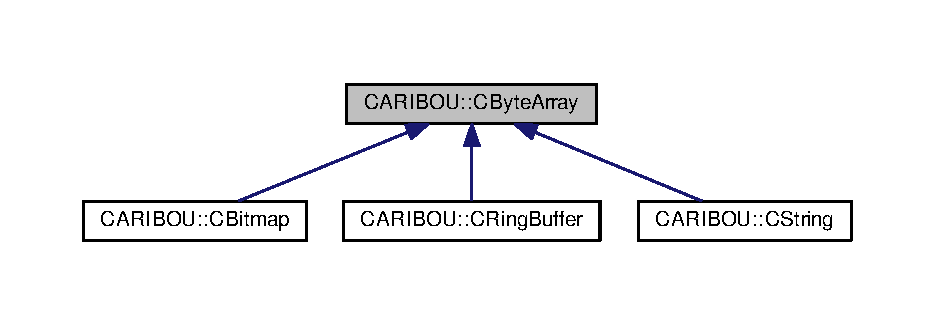
\includegraphics[width=350pt]{class_c_a_r_i_b_o_u_1_1_c_byte_array__inherit__graph}
\end{center}
\end{figure}
\subsection*{Public Member Functions}
\begin{DoxyCompactItemize}
\item 
{\bf C\+Byte\+Array} ()
\item 
{\bf C\+Byte\+Array} (size\+\_\+t {\bf size})
\item 
{\bf C\+Byte\+Array} (const char $\ast${\bf data}, size\+\_\+t {\bf size})
\item 
{\bf C\+Byte\+Array} (const {\bf C\+Byte\+Array} \&other)
\item 
virtual {\bf $\sim$\+C\+Byte\+Array} ()
\item 
virtual void {\bf clear} ()
\item 
virtual size\+\_\+t {\bf resize} (size\+\_\+t {\bf size})
\item 
virtual int {\bf take} (size\+\_\+t index)
\begin{DoxyCompactList}\small\item\em Return the charactwer at the index position and then remove the character from the array. \end{DoxyCompactList}\item 
virtual size\+\_\+t {\bf length} ()
\item 
bool {\bf copy} (const {\bf C\+Byte\+Array} \&other)
\item 
bool {\bf copy} (const char $\ast$src, size\+\_\+t {\bf size})
\item 
bool {\bf append} ({\bf C\+Byte\+Array} \&other)
\item 
bool {\bf append} (const char $\ast$src, size\+\_\+t {\bf size})
\item 
bool {\bf append} (char src)
\item 
bool {\bf prepend} (const char $\ast$src, size\+\_\+t {\bf size})
\begin{DoxyCompactList}\small\item\em Prepend a number of bytes to the beginning of the array. \end{DoxyCompactList}\item 
bool {\bf prepend} (char src)
\item 
{\bf C\+Byte\+Array} \& {\bf remove} (size\+\_\+t index, size\+\_\+t len=1)
\begin{DoxyCompactList}\small\item\em Remove a byte from the array. \end{DoxyCompactList}\item 
bool {\bf insert} (char $\ast$ch, size\+\_\+t pos, size\+\_\+t len)
\begin{DoxyCompactList}\small\item\em Insert a copy of piece of memory. \end{DoxyCompactList}\item 
bool {\bf insert} (char ch, size\+\_\+t pos)
\begin{DoxyCompactList}\small\item\em Insert a byte at the specified pos. \end{DoxyCompactList}\item 
{\bf C\+Byte\+Array} \& {\bf set} (size\+\_\+t index, const char $\ast$src, size\+\_\+t {\bf size})
\item 
char {\bf set} (size\+\_\+t index, uint8\+\_\+t {\bf data})
\begin{DoxyCompactList}\small\item\em Set a byte in memory checking for valid bounds. \end{DoxyCompactList}\item 
{\bf C\+Byte\+Array} \& {\bf fill} (char ch)
\begin{DoxyCompactList}\small\item\em fill with byte. \end{DoxyCompactList}\item 
virtual int {\bf find} (char ch, int index=0)
\item 
size\+\_\+t {\bf size} ()
\item 
char {\bf at} (size\+\_\+t index)
\item 
char $\ast$ {\bf data} ()
\item 
char $\ast$ {\bf data} (size\+\_\+t idx)
\item 
virtual bool {\bf is\+Null} ()
\item 
virtual bool {\bf is\+Empty} ()
\item 
uint8\+\_\+t {\bf nibble} (uint8\+\_\+t ascii\+Char)
\begin{DoxyCompactList}\small\item\em A\+S\+C\+II char to binary nibble. \end{DoxyCompactList}\item 
{\bf C\+Byte\+Array} \& {\bf from\+Ascii\+Hex} (const char $\ast$ascii\+Hex, size\+\_\+t {\bf size})
\begin{DoxyCompactList}\small\item\em Create a bytes buffer from ascii hex string. \end{DoxyCompactList}\item 
bool {\bf operator!=} (const {\bf C\+Byte\+Array} \&other)
\item 
bool {\bf operator==} (const {\bf C\+Byte\+Array} \&other)
\item 
bool {\bf operator==} (const char $\ast$other)
\item 
{\bf C\+Byte\+Array} \& {\bf operator=} (const {\bf C\+Byte\+Array} \&other)
\item 
{\bf C\+Byte\+Array} \& {\bf operator+=} ({\bf C\+Byte\+Array} \&other)
\item 
char {\bf operator[$\,$]} (int n)
\end{DoxyCompactItemize}
\subsection*{Protected Attributes}
\begin{DoxyCompactItemize}
\item 
size\+\_\+t {\bf m\+\_\+size}
\item 
char $\ast$ {\bf m\+\_\+data}
\end{DoxyCompactItemize}


\subsection{Detailed Description}


Definition at line 25 of file cbytearray.\+h.



\subsection{Constructor \& Destructor Documentation}
\index{C\+A\+R\+I\+B\+O\+U\+::\+C\+Byte\+Array@{C\+A\+R\+I\+B\+O\+U\+::\+C\+Byte\+Array}!C\+Byte\+Array@{C\+Byte\+Array}}
\index{C\+Byte\+Array@{C\+Byte\+Array}!C\+A\+R\+I\+B\+O\+U\+::\+C\+Byte\+Array@{C\+A\+R\+I\+B\+O\+U\+::\+C\+Byte\+Array}}
\subsubsection[{C\+Byte\+Array()}]{\setlength{\rightskip}{0pt plus 5cm}C\+A\+R\+I\+B\+O\+U\+::\+C\+Byte\+Array\+::\+C\+Byte\+Array (
\begin{DoxyParamCaption}
{}
\end{DoxyParamCaption}
)}\label{class_c_a_r_i_b_o_u_1_1_c_byte_array_a799f3cd7e4818b8bf82ef82ca35d12a3}


Definition at line 24 of file cbytearray.\+cpp.

\index{C\+A\+R\+I\+B\+O\+U\+::\+C\+Byte\+Array@{C\+A\+R\+I\+B\+O\+U\+::\+C\+Byte\+Array}!C\+Byte\+Array@{C\+Byte\+Array}}
\index{C\+Byte\+Array@{C\+Byte\+Array}!C\+A\+R\+I\+B\+O\+U\+::\+C\+Byte\+Array@{C\+A\+R\+I\+B\+O\+U\+::\+C\+Byte\+Array}}
\subsubsection[{C\+Byte\+Array(size\+\_\+t size)}]{\setlength{\rightskip}{0pt plus 5cm}C\+A\+R\+I\+B\+O\+U\+::\+C\+Byte\+Array\+::\+C\+Byte\+Array (
\begin{DoxyParamCaption}
\item[{size\+\_\+t}]{size}
\end{DoxyParamCaption}
)}\label{class_c_a_r_i_b_o_u_1_1_c_byte_array_a071a848a735b625202fd81b393b778e9}


Definition at line 30 of file cbytearray.\+cpp.

\index{C\+A\+R\+I\+B\+O\+U\+::\+C\+Byte\+Array@{C\+A\+R\+I\+B\+O\+U\+::\+C\+Byte\+Array}!C\+Byte\+Array@{C\+Byte\+Array}}
\index{C\+Byte\+Array@{C\+Byte\+Array}!C\+A\+R\+I\+B\+O\+U\+::\+C\+Byte\+Array@{C\+A\+R\+I\+B\+O\+U\+::\+C\+Byte\+Array}}
\subsubsection[{C\+Byte\+Array(const char $\ast$data, size\+\_\+t size)}]{\setlength{\rightskip}{0pt plus 5cm}C\+A\+R\+I\+B\+O\+U\+::\+C\+Byte\+Array\+::\+C\+Byte\+Array (
\begin{DoxyParamCaption}
\item[{const char $\ast$}]{data, }
\item[{size\+\_\+t}]{size}
\end{DoxyParamCaption}
)}\label{class_c_a_r_i_b_o_u_1_1_c_byte_array_af4e178e15c039d5f5f3d0f70811e0921}


Definition at line 41 of file cbytearray.\+cpp.

\index{C\+A\+R\+I\+B\+O\+U\+::\+C\+Byte\+Array@{C\+A\+R\+I\+B\+O\+U\+::\+C\+Byte\+Array}!C\+Byte\+Array@{C\+Byte\+Array}}
\index{C\+Byte\+Array@{C\+Byte\+Array}!C\+A\+R\+I\+B\+O\+U\+::\+C\+Byte\+Array@{C\+A\+R\+I\+B\+O\+U\+::\+C\+Byte\+Array}}
\subsubsection[{C\+Byte\+Array(const C\+Byte\+Array \&other)}]{\setlength{\rightskip}{0pt plus 5cm}C\+A\+R\+I\+B\+O\+U\+::\+C\+Byte\+Array\+::\+C\+Byte\+Array (
\begin{DoxyParamCaption}
\item[{const {\bf C\+Byte\+Array} \&}]{other}
\end{DoxyParamCaption}
)}\label{class_c_a_r_i_b_o_u_1_1_c_byte_array_a8e6128239925046d2f319f474ecae454}


Definition at line 51 of file cbytearray.\+cpp.

\index{C\+A\+R\+I\+B\+O\+U\+::\+C\+Byte\+Array@{C\+A\+R\+I\+B\+O\+U\+::\+C\+Byte\+Array}!````~C\+Byte\+Array@{$\sim$\+C\+Byte\+Array}}
\index{````~C\+Byte\+Array@{$\sim$\+C\+Byte\+Array}!C\+A\+R\+I\+B\+O\+U\+::\+C\+Byte\+Array@{C\+A\+R\+I\+B\+O\+U\+::\+C\+Byte\+Array}}
\subsubsection[{$\sim$\+C\+Byte\+Array()}]{\setlength{\rightskip}{0pt plus 5cm}C\+A\+R\+I\+B\+O\+U\+::\+C\+Byte\+Array\+::$\sim$\+C\+Byte\+Array (
\begin{DoxyParamCaption}
{}
\end{DoxyParamCaption}
)\hspace{0.3cm}{\ttfamily [virtual]}}\label{class_c_a_r_i_b_o_u_1_1_c_byte_array_ad565792af7d42b65690fb77e16836187}


Definition at line 58 of file cbytearray.\+cpp.



\subsection{Member Function Documentation}
\index{C\+A\+R\+I\+B\+O\+U\+::\+C\+Byte\+Array@{C\+A\+R\+I\+B\+O\+U\+::\+C\+Byte\+Array}!append@{append}}
\index{append@{append}!C\+A\+R\+I\+B\+O\+U\+::\+C\+Byte\+Array@{C\+A\+R\+I\+B\+O\+U\+::\+C\+Byte\+Array}}
\subsubsection[{append(\+C\+Byte\+Array \&other)}]{\setlength{\rightskip}{0pt plus 5cm}bool C\+A\+R\+I\+B\+O\+U\+::\+C\+Byte\+Array\+::append (
\begin{DoxyParamCaption}
\item[{{\bf C\+Byte\+Array} \&}]{other}
\end{DoxyParamCaption}
)}\label{class_c_a_r_i_b_o_u_1_1_c_byte_array_a187b00bab8236a29fca6ca659632a3d8}


Definition at line 108 of file cbytearray.\+cpp.

\index{C\+A\+R\+I\+B\+O\+U\+::\+C\+Byte\+Array@{C\+A\+R\+I\+B\+O\+U\+::\+C\+Byte\+Array}!append@{append}}
\index{append@{append}!C\+A\+R\+I\+B\+O\+U\+::\+C\+Byte\+Array@{C\+A\+R\+I\+B\+O\+U\+::\+C\+Byte\+Array}}
\subsubsection[{append(const char $\ast$src, size\+\_\+t size)}]{\setlength{\rightskip}{0pt plus 5cm}bool C\+A\+R\+I\+B\+O\+U\+::\+C\+Byte\+Array\+::append (
\begin{DoxyParamCaption}
\item[{const char $\ast$}]{src, }
\item[{size\+\_\+t}]{size}
\end{DoxyParamCaption}
)}\label{class_c_a_r_i_b_o_u_1_1_c_byte_array_ae8a9c26cbd5c681b435224276940e057}


Definition at line 113 of file cbytearray.\+cpp.

\index{C\+A\+R\+I\+B\+O\+U\+::\+C\+Byte\+Array@{C\+A\+R\+I\+B\+O\+U\+::\+C\+Byte\+Array}!append@{append}}
\index{append@{append}!C\+A\+R\+I\+B\+O\+U\+::\+C\+Byte\+Array@{C\+A\+R\+I\+B\+O\+U\+::\+C\+Byte\+Array}}
\subsubsection[{append(char src)}]{\setlength{\rightskip}{0pt plus 5cm}bool C\+A\+R\+I\+B\+O\+U\+::\+C\+Byte\+Array\+::append (
\begin{DoxyParamCaption}
\item[{char}]{src}
\end{DoxyParamCaption}
)}\label{class_c_a_r_i_b_o_u_1_1_c_byte_array_ab62b1372813d5a5c201acf4f493ab6c0}


Definition at line 103 of file cbytearray.\+cpp.

\index{C\+A\+R\+I\+B\+O\+U\+::\+C\+Byte\+Array@{C\+A\+R\+I\+B\+O\+U\+::\+C\+Byte\+Array}!at@{at}}
\index{at@{at}!C\+A\+R\+I\+B\+O\+U\+::\+C\+Byte\+Array@{C\+A\+R\+I\+B\+O\+U\+::\+C\+Byte\+Array}}
\subsubsection[{at(size\+\_\+t index)}]{\setlength{\rightskip}{0pt plus 5cm}char C\+A\+R\+I\+B\+O\+U\+::\+C\+Byte\+Array\+::at (
\begin{DoxyParamCaption}
\item[{size\+\_\+t}]{index}
\end{DoxyParamCaption}
)\hspace{0.3cm}{\ttfamily [inline]}}\label{class_c_a_r_i_b_o_u_1_1_c_byte_array_ab26c295c50bb649e0fb3fddf71b79c24}


Definition at line 55 of file cbytearray.\+h.

\index{C\+A\+R\+I\+B\+O\+U\+::\+C\+Byte\+Array@{C\+A\+R\+I\+B\+O\+U\+::\+C\+Byte\+Array}!clear@{clear}}
\index{clear@{clear}!C\+A\+R\+I\+B\+O\+U\+::\+C\+Byte\+Array@{C\+A\+R\+I\+B\+O\+U\+::\+C\+Byte\+Array}}
\subsubsection[{clear()}]{\setlength{\rightskip}{0pt plus 5cm}void C\+A\+R\+I\+B\+O\+U\+::\+C\+Byte\+Array\+::clear (
\begin{DoxyParamCaption}
{}
\end{DoxyParamCaption}
)\hspace{0.3cm}{\ttfamily [virtual]}}\label{class_c_a_r_i_b_o_u_1_1_c_byte_array_a21a6406374c2f76a71e3a1f038dbf31a}


Reimplemented in {\bf C\+A\+R\+I\+B\+O\+U\+::\+C\+Bitmap} \doxyref{}{p.}{class_c_a_r_i_b_o_u_1_1_c_bitmap_abde5f3ea3c04afd596d13f58f8de06db}, and {\bf C\+A\+R\+I\+B\+O\+U\+::\+C\+Ring\+Buffer} \doxyref{}{p.}{class_c_a_r_i_b_o_u_1_1_c_ring_buffer_acf387649e99034ef25a6fb5cd40edd3a}.



Definition at line 63 of file cbytearray.\+cpp.

\index{C\+A\+R\+I\+B\+O\+U\+::\+C\+Byte\+Array@{C\+A\+R\+I\+B\+O\+U\+::\+C\+Byte\+Array}!copy@{copy}}
\index{copy@{copy}!C\+A\+R\+I\+B\+O\+U\+::\+C\+Byte\+Array@{C\+A\+R\+I\+B\+O\+U\+::\+C\+Byte\+Array}}
\subsubsection[{copy(const C\+Byte\+Array \&other)}]{\setlength{\rightskip}{0pt plus 5cm}bool C\+A\+R\+I\+B\+O\+U\+::\+C\+Byte\+Array\+::copy (
\begin{DoxyParamCaption}
\item[{const {\bf C\+Byte\+Array} \&}]{other}
\end{DoxyParamCaption}
)}\label{class_c_a_r_i_b_o_u_1_1_c_byte_array_a8517dd73a3bd27ed6f3b317788a1f471}


Definition at line 140 of file cbytearray.\+cpp.

\index{C\+A\+R\+I\+B\+O\+U\+::\+C\+Byte\+Array@{C\+A\+R\+I\+B\+O\+U\+::\+C\+Byte\+Array}!copy@{copy}}
\index{copy@{copy}!C\+A\+R\+I\+B\+O\+U\+::\+C\+Byte\+Array@{C\+A\+R\+I\+B\+O\+U\+::\+C\+Byte\+Array}}
\subsubsection[{copy(const char $\ast$src, size\+\_\+t size)}]{\setlength{\rightskip}{0pt plus 5cm}bool C\+A\+R\+I\+B\+O\+U\+::\+C\+Byte\+Array\+::copy (
\begin{DoxyParamCaption}
\item[{const char $\ast$}]{src, }
\item[{size\+\_\+t}]{size}
\end{DoxyParamCaption}
)}\label{class_c_a_r_i_b_o_u_1_1_c_byte_array_a3b6bba040fc2557f54194f4b7c7d2c8c}


Definition at line 130 of file cbytearray.\+cpp.

\index{C\+A\+R\+I\+B\+O\+U\+::\+C\+Byte\+Array@{C\+A\+R\+I\+B\+O\+U\+::\+C\+Byte\+Array}!data@{data}}
\index{data@{data}!C\+A\+R\+I\+B\+O\+U\+::\+C\+Byte\+Array@{C\+A\+R\+I\+B\+O\+U\+::\+C\+Byte\+Array}}
\subsubsection[{data()}]{\setlength{\rightskip}{0pt plus 5cm}char$\ast$ C\+A\+R\+I\+B\+O\+U\+::\+C\+Byte\+Array\+::data (
\begin{DoxyParamCaption}
{}
\end{DoxyParamCaption}
)\hspace{0.3cm}{\ttfamily [inline]}}\label{class_c_a_r_i_b_o_u_1_1_c_byte_array_af96d08dac45a219528e1e5c97fd16a7e}


Definition at line 56 of file cbytearray.\+h.

\index{C\+A\+R\+I\+B\+O\+U\+::\+C\+Byte\+Array@{C\+A\+R\+I\+B\+O\+U\+::\+C\+Byte\+Array}!data@{data}}
\index{data@{data}!C\+A\+R\+I\+B\+O\+U\+::\+C\+Byte\+Array@{C\+A\+R\+I\+B\+O\+U\+::\+C\+Byte\+Array}}
\subsubsection[{data(size\+\_\+t idx)}]{\setlength{\rightskip}{0pt plus 5cm}char$\ast$ C\+A\+R\+I\+B\+O\+U\+::\+C\+Byte\+Array\+::data (
\begin{DoxyParamCaption}
\item[{size\+\_\+t}]{idx}
\end{DoxyParamCaption}
)\hspace{0.3cm}{\ttfamily [inline]}}\label{class_c_a_r_i_b_o_u_1_1_c_byte_array_a589c6c8b4b2a793bf657b1e8b5e0cc56}


Definition at line 57 of file cbytearray.\+h.

\index{C\+A\+R\+I\+B\+O\+U\+::\+C\+Byte\+Array@{C\+A\+R\+I\+B\+O\+U\+::\+C\+Byte\+Array}!fill@{fill}}
\index{fill@{fill}!C\+A\+R\+I\+B\+O\+U\+::\+C\+Byte\+Array@{C\+A\+R\+I\+B\+O\+U\+::\+C\+Byte\+Array}}
\subsubsection[{fill(char ch)}]{\setlength{\rightskip}{0pt plus 5cm}{\bf C\+Byte\+Array} \& C\+A\+R\+I\+B\+O\+U\+::\+C\+Byte\+Array\+::fill (
\begin{DoxyParamCaption}
\item[{char}]{ch}
\end{DoxyParamCaption}
)}\label{class_c_a_r_i_b_o_u_1_1_c_byte_array_a9246c101a8caed7e8bb9ecfc4ac4614c}


fill with byte. 



Definition at line 200 of file cbytearray.\+cpp.

\index{C\+A\+R\+I\+B\+O\+U\+::\+C\+Byte\+Array@{C\+A\+R\+I\+B\+O\+U\+::\+C\+Byte\+Array}!find@{find}}
\index{find@{find}!C\+A\+R\+I\+B\+O\+U\+::\+C\+Byte\+Array@{C\+A\+R\+I\+B\+O\+U\+::\+C\+Byte\+Array}}
\subsubsection[{find(char ch, int index=0)}]{\setlength{\rightskip}{0pt plus 5cm}int C\+A\+R\+I\+B\+O\+U\+::\+C\+Byte\+Array\+::find (
\begin{DoxyParamCaption}
\item[{char}]{ch, }
\item[{int}]{index = {\ttfamily 0}}
\end{DoxyParamCaption}
)\hspace{0.3cm}{\ttfamily [virtual]}}\label{class_c_a_r_i_b_o_u_1_1_c_byte_array_ae5d3e1caeb5bac36c9c16c5717eb9b92}


Reimplemented in {\bf C\+A\+R\+I\+B\+O\+U\+::\+C\+String} \doxyref{}{p.}{class_c_a_r_i_b_o_u_1_1_c_string_ace2cc77dc0b4f32ae63ce51bd2791fab}.



Definition at line 296 of file cbytearray.\+cpp.

\index{C\+A\+R\+I\+B\+O\+U\+::\+C\+Byte\+Array@{C\+A\+R\+I\+B\+O\+U\+::\+C\+Byte\+Array}!from\+Ascii\+Hex@{from\+Ascii\+Hex}}
\index{from\+Ascii\+Hex@{from\+Ascii\+Hex}!C\+A\+R\+I\+B\+O\+U\+::\+C\+Byte\+Array@{C\+A\+R\+I\+B\+O\+U\+::\+C\+Byte\+Array}}
\subsubsection[{from\+Ascii\+Hex(const char $\ast$ascii\+Hex, size\+\_\+t size)}]{\setlength{\rightskip}{0pt plus 5cm}{\bf C\+Byte\+Array} \& C\+A\+R\+I\+B\+O\+U\+::\+C\+Byte\+Array\+::from\+Ascii\+Hex (
\begin{DoxyParamCaption}
\item[{const char $\ast$}]{ascii\+Hex, }
\item[{size\+\_\+t}]{size}
\end{DoxyParamCaption}
)}\label{class_c_a_r_i_b_o_u_1_1_c_byte_array_a88917f7e29df8df73793181e9446283f}


Create a bytes buffer from ascii hex string. 



Definition at line 339 of file cbytearray.\+cpp.

\index{C\+A\+R\+I\+B\+O\+U\+::\+C\+Byte\+Array@{C\+A\+R\+I\+B\+O\+U\+::\+C\+Byte\+Array}!insert@{insert}}
\index{insert@{insert}!C\+A\+R\+I\+B\+O\+U\+::\+C\+Byte\+Array@{C\+A\+R\+I\+B\+O\+U\+::\+C\+Byte\+Array}}
\subsubsection[{insert(char $\ast$ch, size\+\_\+t pos, size\+\_\+t len)}]{\setlength{\rightskip}{0pt plus 5cm}bool C\+A\+R\+I\+B\+O\+U\+::\+C\+Byte\+Array\+::insert (
\begin{DoxyParamCaption}
\item[{char $\ast$}]{ch, }
\item[{size\+\_\+t}]{pos, }
\item[{size\+\_\+t}]{len}
\end{DoxyParamCaption}
)}\label{class_c_a_r_i_b_o_u_1_1_c_byte_array_a62d2fd26e4b1b5e682b1bd7e06587adc}


Insert a copy of piece of memory. 



Definition at line 260 of file cbytearray.\+cpp.

\index{C\+A\+R\+I\+B\+O\+U\+::\+C\+Byte\+Array@{C\+A\+R\+I\+B\+O\+U\+::\+C\+Byte\+Array}!insert@{insert}}
\index{insert@{insert}!C\+A\+R\+I\+B\+O\+U\+::\+C\+Byte\+Array@{C\+A\+R\+I\+B\+O\+U\+::\+C\+Byte\+Array}}
\subsubsection[{insert(char ch, size\+\_\+t pos)}]{\setlength{\rightskip}{0pt plus 5cm}bool C\+A\+R\+I\+B\+O\+U\+::\+C\+Byte\+Array\+::insert (
\begin{DoxyParamCaption}
\item[{char}]{ch, }
\item[{size\+\_\+t}]{pos}
\end{DoxyParamCaption}
)}\label{class_c_a_r_i_b_o_u_1_1_c_byte_array_abd7d08eab8e561acb2c388f3a2c7c8ed}


Insert a byte at the specified pos. 



Definition at line 252 of file cbytearray.\+cpp.

\index{C\+A\+R\+I\+B\+O\+U\+::\+C\+Byte\+Array@{C\+A\+R\+I\+B\+O\+U\+::\+C\+Byte\+Array}!is\+Empty@{is\+Empty}}
\index{is\+Empty@{is\+Empty}!C\+A\+R\+I\+B\+O\+U\+::\+C\+Byte\+Array@{C\+A\+R\+I\+B\+O\+U\+::\+C\+Byte\+Array}}
\subsubsection[{is\+Empty()}]{\setlength{\rightskip}{0pt plus 5cm}virtual bool C\+A\+R\+I\+B\+O\+U\+::\+C\+Byte\+Array\+::is\+Empty (
\begin{DoxyParamCaption}
{}
\end{DoxyParamCaption}
)\hspace{0.3cm}{\ttfamily [inline]}, {\ttfamily [virtual]}}\label{class_c_a_r_i_b_o_u_1_1_c_byte_array_a59e1c2b03d5975af7f2a31768ca79c0f}


Reimplemented in {\bf C\+A\+R\+I\+B\+O\+U\+::\+C\+String} \doxyref{}{p.}{class_c_a_r_i_b_o_u_1_1_c_string_ad7dac8402fc1bbacbeeb8ef4e8cad9e7}.



Definition at line 60 of file cbytearray.\+h.

\index{C\+A\+R\+I\+B\+O\+U\+::\+C\+Byte\+Array@{C\+A\+R\+I\+B\+O\+U\+::\+C\+Byte\+Array}!is\+Null@{is\+Null}}
\index{is\+Null@{is\+Null}!C\+A\+R\+I\+B\+O\+U\+::\+C\+Byte\+Array@{C\+A\+R\+I\+B\+O\+U\+::\+C\+Byte\+Array}}
\subsubsection[{is\+Null()}]{\setlength{\rightskip}{0pt plus 5cm}virtual bool C\+A\+R\+I\+B\+O\+U\+::\+C\+Byte\+Array\+::is\+Null (
\begin{DoxyParamCaption}
{}
\end{DoxyParamCaption}
)\hspace{0.3cm}{\ttfamily [inline]}, {\ttfamily [virtual]}}\label{class_c_a_r_i_b_o_u_1_1_c_byte_array_a465f0cc0478168743f052883cfa44ec2}


Definition at line 59 of file cbytearray.\+h.

\index{C\+A\+R\+I\+B\+O\+U\+::\+C\+Byte\+Array@{C\+A\+R\+I\+B\+O\+U\+::\+C\+Byte\+Array}!length@{length}}
\index{length@{length}!C\+A\+R\+I\+B\+O\+U\+::\+C\+Byte\+Array@{C\+A\+R\+I\+B\+O\+U\+::\+C\+Byte\+Array}}
\subsubsection[{length()}]{\setlength{\rightskip}{0pt plus 5cm}size\+\_\+t C\+A\+R\+I\+B\+O\+U\+::\+C\+Byte\+Array\+::length (
\begin{DoxyParamCaption}
{}
\end{DoxyParamCaption}
)\hspace{0.3cm}{\ttfamily [virtual]}}\label{class_c_a_r_i_b_o_u_1_1_c_byte_array_ad15b129f7a5169d87c90b9ec14a7f285}


Reimplemented in {\bf C\+A\+R\+I\+B\+O\+U\+::\+C\+String} \doxyref{}{p.}{class_c_a_r_i_b_o_u_1_1_c_string_af371807705dbd4011789503ca149cd07}, and {\bf C\+A\+R\+I\+B\+O\+U\+::\+C\+Ring\+Buffer} \doxyref{}{p.}{class_c_a_r_i_b_o_u_1_1_c_ring_buffer_a0912316591e34c5d6d608397e89f1475}.



Definition at line 291 of file cbytearray.\+cpp.

\index{C\+A\+R\+I\+B\+O\+U\+::\+C\+Byte\+Array@{C\+A\+R\+I\+B\+O\+U\+::\+C\+Byte\+Array}!nibble@{nibble}}
\index{nibble@{nibble}!C\+A\+R\+I\+B\+O\+U\+::\+C\+Byte\+Array@{C\+A\+R\+I\+B\+O\+U\+::\+C\+Byte\+Array}}
\subsubsection[{nibble(uint8\+\_\+t ascii\+Char)}]{\setlength{\rightskip}{0pt plus 5cm}uint8\+\_\+t C\+A\+R\+I\+B\+O\+U\+::\+C\+Byte\+Array\+::nibble (
\begin{DoxyParamCaption}
\item[{uint8\+\_\+t}]{ascii\+Char}
\end{DoxyParamCaption}
)}\label{class_c_a_r_i_b_o_u_1_1_c_byte_array_a8f140f828e796d03f6d2879064b6cd44}


A\+S\+C\+II char to binary nibble. 



Definition at line 312 of file cbytearray.\+cpp.

\index{C\+A\+R\+I\+B\+O\+U\+::\+C\+Byte\+Array@{C\+A\+R\+I\+B\+O\+U\+::\+C\+Byte\+Array}!operator"!=@{operator"!=}}
\index{operator"!=@{operator"!=}!C\+A\+R\+I\+B\+O\+U\+::\+C\+Byte\+Array@{C\+A\+R\+I\+B\+O\+U\+::\+C\+Byte\+Array}}
\subsubsection[{operator"!=(const C\+Byte\+Array \&other)}]{\setlength{\rightskip}{0pt plus 5cm}bool C\+A\+R\+I\+B\+O\+U\+::\+C\+Byte\+Array\+::operator!= (
\begin{DoxyParamCaption}
\item[{const {\bf C\+Byte\+Array} \&}]{other}
\end{DoxyParamCaption}
)\hspace{0.3cm}{\ttfamily [inline]}}\label{class_c_a_r_i_b_o_u_1_1_c_byte_array_a56f3f3dde8a73c9c9c763648e99ffce3}


Definition at line 65 of file cbytearray.\+h.

\index{C\+A\+R\+I\+B\+O\+U\+::\+C\+Byte\+Array@{C\+A\+R\+I\+B\+O\+U\+::\+C\+Byte\+Array}!operator+=@{operator+=}}
\index{operator+=@{operator+=}!C\+A\+R\+I\+B\+O\+U\+::\+C\+Byte\+Array@{C\+A\+R\+I\+B\+O\+U\+::\+C\+Byte\+Array}}
\subsubsection[{operator+=(\+C\+Byte\+Array \&other)}]{\setlength{\rightskip}{0pt plus 5cm}{\bf C\+Byte\+Array}\& C\+A\+R\+I\+B\+O\+U\+::\+C\+Byte\+Array\+::operator+= (
\begin{DoxyParamCaption}
\item[{{\bf C\+Byte\+Array} \&}]{other}
\end{DoxyParamCaption}
)\hspace{0.3cm}{\ttfamily [inline]}}\label{class_c_a_r_i_b_o_u_1_1_c_byte_array_a55b36e61eafe84a92e1f645071d84294}


Definition at line 69 of file cbytearray.\+h.

\index{C\+A\+R\+I\+B\+O\+U\+::\+C\+Byte\+Array@{C\+A\+R\+I\+B\+O\+U\+::\+C\+Byte\+Array}!operator=@{operator=}}
\index{operator=@{operator=}!C\+A\+R\+I\+B\+O\+U\+::\+C\+Byte\+Array@{C\+A\+R\+I\+B\+O\+U\+::\+C\+Byte\+Array}}
\subsubsection[{operator=(const C\+Byte\+Array \&other)}]{\setlength{\rightskip}{0pt plus 5cm}{\bf C\+Byte\+Array}\& C\+A\+R\+I\+B\+O\+U\+::\+C\+Byte\+Array\+::operator= (
\begin{DoxyParamCaption}
\item[{const {\bf C\+Byte\+Array} \&}]{other}
\end{DoxyParamCaption}
)\hspace{0.3cm}{\ttfamily [inline]}}\label{class_c_a_r_i_b_o_u_1_1_c_byte_array_a5361cc05ddea67ed3fe358ac7888fc82}


Definition at line 68 of file cbytearray.\+h.

\index{C\+A\+R\+I\+B\+O\+U\+::\+C\+Byte\+Array@{C\+A\+R\+I\+B\+O\+U\+::\+C\+Byte\+Array}!operator==@{operator==}}
\index{operator==@{operator==}!C\+A\+R\+I\+B\+O\+U\+::\+C\+Byte\+Array@{C\+A\+R\+I\+B\+O\+U\+::\+C\+Byte\+Array}}
\subsubsection[{operator==(const C\+Byte\+Array \&other)}]{\setlength{\rightskip}{0pt plus 5cm}bool C\+A\+R\+I\+B\+O\+U\+::\+C\+Byte\+Array\+::operator== (
\begin{DoxyParamCaption}
\item[{const {\bf C\+Byte\+Array} \&}]{other}
\end{DoxyParamCaption}
)}\label{class_c_a_r_i_b_o_u_1_1_c_byte_array_a92ceab67ab68fb3013a8107df2c5f680}


Definition at line 79 of file cbytearray.\+cpp.

\index{C\+A\+R\+I\+B\+O\+U\+::\+C\+Byte\+Array@{C\+A\+R\+I\+B\+O\+U\+::\+C\+Byte\+Array}!operator==@{operator==}}
\index{operator==@{operator==}!C\+A\+R\+I\+B\+O\+U\+::\+C\+Byte\+Array@{C\+A\+R\+I\+B\+O\+U\+::\+C\+Byte\+Array}}
\subsubsection[{operator==(const char $\ast$other)}]{\setlength{\rightskip}{0pt plus 5cm}bool C\+A\+R\+I\+B\+O\+U\+::\+C\+Byte\+Array\+::operator== (
\begin{DoxyParamCaption}
\item[{const char $\ast$}]{other}
\end{DoxyParamCaption}
)}\label{class_c_a_r_i_b_o_u_1_1_c_byte_array_a91fd4ea9197acf0a4339b4ad4b8c3f10}


Definition at line 73 of file cbytearray.\+cpp.

\index{C\+A\+R\+I\+B\+O\+U\+::\+C\+Byte\+Array@{C\+A\+R\+I\+B\+O\+U\+::\+C\+Byte\+Array}!operator[$\,$]@{operator[]}}
\index{operator[$\,$]@{operator[]}!C\+A\+R\+I\+B\+O\+U\+::\+C\+Byte\+Array@{C\+A\+R\+I\+B\+O\+U\+::\+C\+Byte\+Array}}
\subsubsection[{operator[](int n)}]{\setlength{\rightskip}{0pt plus 5cm}char C\+A\+R\+I\+B\+O\+U\+::\+C\+Byte\+Array\+::operator[$\,$] (
\begin{DoxyParamCaption}
\item[{int}]{n}
\end{DoxyParamCaption}
)\hspace{0.3cm}{\ttfamily [inline]}}\label{class_c_a_r_i_b_o_u_1_1_c_byte_array_a10767ebe31c965d50cad4dcdc7369ef2}


Definition at line 70 of file cbytearray.\+h.

\index{C\+A\+R\+I\+B\+O\+U\+::\+C\+Byte\+Array@{C\+A\+R\+I\+B\+O\+U\+::\+C\+Byte\+Array}!prepend@{prepend}}
\index{prepend@{prepend}!C\+A\+R\+I\+B\+O\+U\+::\+C\+Byte\+Array@{C\+A\+R\+I\+B\+O\+U\+::\+C\+Byte\+Array}}
\subsubsection[{prepend(const char $\ast$src, size\+\_\+t size)}]{\setlength{\rightskip}{0pt plus 5cm}bool C\+A\+R\+I\+B\+O\+U\+::\+C\+Byte\+Array\+::prepend (
\begin{DoxyParamCaption}
\item[{const char $\ast$}]{data, }
\item[{size\+\_\+t}]{size}
\end{DoxyParamCaption}
)}\label{class_c_a_r_i_b_o_u_1_1_c_byte_array_a835b10fab570b39aede0436b3955e78f}


Prepend a number of bytes to the beginning of the array. 


\begin{DoxyParams}{Parameters}
{\em data} & The bytes to prepend. \\
\hline
{\em size} & The number of bytes to prepend \\
\hline
\end{DoxyParams}


Definition at line 214 of file cbytearray.\+cpp.

\index{C\+A\+R\+I\+B\+O\+U\+::\+C\+Byte\+Array@{C\+A\+R\+I\+B\+O\+U\+::\+C\+Byte\+Array}!prepend@{prepend}}
\index{prepend@{prepend}!C\+A\+R\+I\+B\+O\+U\+::\+C\+Byte\+Array@{C\+A\+R\+I\+B\+O\+U\+::\+C\+Byte\+Array}}
\subsubsection[{prepend(char src)}]{\setlength{\rightskip}{0pt plus 5cm}bool C\+A\+R\+I\+B\+O\+U\+::\+C\+Byte\+Array\+::prepend (
\begin{DoxyParamCaption}
\item[{char}]{src}
\end{DoxyParamCaption}
)}\label{class_c_a_r_i_b_o_u_1_1_c_byte_array_a77c194cfb09d4e9265d15dce72654f66}


Definition at line 226 of file cbytearray.\+cpp.

\index{C\+A\+R\+I\+B\+O\+U\+::\+C\+Byte\+Array@{C\+A\+R\+I\+B\+O\+U\+::\+C\+Byte\+Array}!remove@{remove}}
\index{remove@{remove}!C\+A\+R\+I\+B\+O\+U\+::\+C\+Byte\+Array@{C\+A\+R\+I\+B\+O\+U\+::\+C\+Byte\+Array}}
\subsubsection[{remove(size\+\_\+t index, size\+\_\+t len=1)}]{\setlength{\rightskip}{0pt plus 5cm}{\bf C\+Byte\+Array} \& C\+A\+R\+I\+B\+O\+U\+::\+C\+Byte\+Array\+::remove (
\begin{DoxyParamCaption}
\item[{size\+\_\+t}]{index, }
\item[{size\+\_\+t}]{len = {\ttfamily 1}}
\end{DoxyParamCaption}
)}\label{class_c_a_r_i_b_o_u_1_1_c_byte_array_a6a09010e3ec1cc6b046e1b89ee12c599}


Remove a byte from the array. 

The following bytes are shifted left. 
\begin{DoxyParams}{Parameters}
{\em index} & The index of the byte to remove. \\
\hline
{\em len} & the number of bytes to remove \\
\hline
\end{DoxyParams}


Definition at line 236 of file cbytearray.\+cpp.

\index{C\+A\+R\+I\+B\+O\+U\+::\+C\+Byte\+Array@{C\+A\+R\+I\+B\+O\+U\+::\+C\+Byte\+Array}!resize@{resize}}
\index{resize@{resize}!C\+A\+R\+I\+B\+O\+U\+::\+C\+Byte\+Array@{C\+A\+R\+I\+B\+O\+U\+::\+C\+Byte\+Array}}
\subsubsection[{resize(size\+\_\+t size)}]{\setlength{\rightskip}{0pt plus 5cm}size\+\_\+t C\+A\+R\+I\+B\+O\+U\+::\+C\+Byte\+Array\+::resize (
\begin{DoxyParamCaption}
\item[{size\+\_\+t}]{size}
\end{DoxyParamCaption}
)\hspace{0.3cm}{\ttfamily [virtual]}}\label{class_c_a_r_i_b_o_u_1_1_c_byte_array_ad9a01a668ed71959fe1539dd77b9223e}


Reimplemented in {\bf C\+A\+R\+I\+B\+O\+U\+::\+C\+String} \doxyref{}{p.}{class_c_a_r_i_b_o_u_1_1_c_string_adebdf6c793e7be876b4114e7fa3afa29}, and {\bf C\+A\+R\+I\+B\+O\+U\+::\+C\+Ring\+Buffer} \doxyref{}{p.}{class_c_a_r_i_b_o_u_1_1_c_ring_buffer_a2802c6bc5f7bd6eb460f970d18676700}.



Definition at line 146 of file cbytearray.\+cpp.

\index{C\+A\+R\+I\+B\+O\+U\+::\+C\+Byte\+Array@{C\+A\+R\+I\+B\+O\+U\+::\+C\+Byte\+Array}!set@{set}}
\index{set@{set}!C\+A\+R\+I\+B\+O\+U\+::\+C\+Byte\+Array@{C\+A\+R\+I\+B\+O\+U\+::\+C\+Byte\+Array}}
\subsubsection[{set(size\+\_\+t index, const char $\ast$src, size\+\_\+t size)}]{\setlength{\rightskip}{0pt plus 5cm}{\bf C\+Byte\+Array} \& C\+A\+R\+I\+B\+O\+U\+::\+C\+Byte\+Array\+::set (
\begin{DoxyParamCaption}
\item[{size\+\_\+t}]{index, }
\item[{const char $\ast$}]{src, }
\item[{size\+\_\+t}]{size}
\end{DoxyParamCaption}
)}\label{class_c_a_r_i_b_o_u_1_1_c_byte_array_a2941d1937537a4da6d2ca4d27b38a7d2}


Definition at line 170 of file cbytearray.\+cpp.

\index{C\+A\+R\+I\+B\+O\+U\+::\+C\+Byte\+Array@{C\+A\+R\+I\+B\+O\+U\+::\+C\+Byte\+Array}!set@{set}}
\index{set@{set}!C\+A\+R\+I\+B\+O\+U\+::\+C\+Byte\+Array@{C\+A\+R\+I\+B\+O\+U\+::\+C\+Byte\+Array}}
\subsubsection[{set(size\+\_\+t index, uint8\+\_\+t data)}]{\setlength{\rightskip}{0pt plus 5cm}char C\+A\+R\+I\+B\+O\+U\+::\+C\+Byte\+Array\+::set (
\begin{DoxyParamCaption}
\item[{size\+\_\+t}]{index, }
\item[{uint8\+\_\+t}]{data}
\end{DoxyParamCaption}
)}\label{class_c_a_r_i_b_o_u_1_1_c_byte_array_a81bf25a7b5bf4b0568539fb82cae24f3}


Set a byte in memory checking for valid bounds. 



Definition at line 182 of file cbytearray.\+cpp.

\index{C\+A\+R\+I\+B\+O\+U\+::\+C\+Byte\+Array@{C\+A\+R\+I\+B\+O\+U\+::\+C\+Byte\+Array}!size@{size}}
\index{size@{size}!C\+A\+R\+I\+B\+O\+U\+::\+C\+Byte\+Array@{C\+A\+R\+I\+B\+O\+U\+::\+C\+Byte\+Array}}
\subsubsection[{size()}]{\setlength{\rightskip}{0pt plus 5cm}size\+\_\+t C\+A\+R\+I\+B\+O\+U\+::\+C\+Byte\+Array\+::size (
\begin{DoxyParamCaption}
{}
\end{DoxyParamCaption}
)\hspace{0.3cm}{\ttfamily [inline]}}\label{class_c_a_r_i_b_o_u_1_1_c_byte_array_a6ea44ee589e1ef1ed723b96af0ecf1d4}


Definition at line 54 of file cbytearray.\+h.

\index{C\+A\+R\+I\+B\+O\+U\+::\+C\+Byte\+Array@{C\+A\+R\+I\+B\+O\+U\+::\+C\+Byte\+Array}!take@{take}}
\index{take@{take}!C\+A\+R\+I\+B\+O\+U\+::\+C\+Byte\+Array@{C\+A\+R\+I\+B\+O\+U\+::\+C\+Byte\+Array}}
\subsubsection[{take(size\+\_\+t index)}]{\setlength{\rightskip}{0pt plus 5cm}int C\+A\+R\+I\+B\+O\+U\+::\+C\+Byte\+Array\+::take (
\begin{DoxyParamCaption}
\item[{size\+\_\+t}]{index}
\end{DoxyParamCaption}
)\hspace{0.3cm}{\ttfamily [virtual]}}\label{class_c_a_r_i_b_o_u_1_1_c_byte_array_a5adaaa78ca503a96f69fa24d85960fc9}


Return the charactwer at the index position and then remove the character from the array. 

\begin{DoxyReturn}{Returns}
the character at the index position of -\/1 if out of range. 
\end{DoxyReturn}


Definition at line 280 of file cbytearray.\+cpp.



\subsection{Member Data Documentation}
\index{C\+A\+R\+I\+B\+O\+U\+::\+C\+Byte\+Array@{C\+A\+R\+I\+B\+O\+U\+::\+C\+Byte\+Array}!m\+\_\+data@{m\+\_\+data}}
\index{m\+\_\+data@{m\+\_\+data}!C\+A\+R\+I\+B\+O\+U\+::\+C\+Byte\+Array@{C\+A\+R\+I\+B\+O\+U\+::\+C\+Byte\+Array}}
\subsubsection[{m\+\_\+data}]{\setlength{\rightskip}{0pt plus 5cm}char$\ast$ C\+A\+R\+I\+B\+O\+U\+::\+C\+Byte\+Array\+::m\+\_\+data\hspace{0.3cm}{\ttfamily [protected]}}\label{class_c_a_r_i_b_o_u_1_1_c_byte_array_aedc488e483b568af7572df965e541634}


Definition at line 75 of file cbytearray.\+h.

\index{C\+A\+R\+I\+B\+O\+U\+::\+C\+Byte\+Array@{C\+A\+R\+I\+B\+O\+U\+::\+C\+Byte\+Array}!m\+\_\+size@{m\+\_\+size}}
\index{m\+\_\+size@{m\+\_\+size}!C\+A\+R\+I\+B\+O\+U\+::\+C\+Byte\+Array@{C\+A\+R\+I\+B\+O\+U\+::\+C\+Byte\+Array}}
\subsubsection[{m\+\_\+size}]{\setlength{\rightskip}{0pt plus 5cm}size\+\_\+t C\+A\+R\+I\+B\+O\+U\+::\+C\+Byte\+Array\+::m\+\_\+size\hspace{0.3cm}{\ttfamily [protected]}}\label{class_c_a_r_i_b_o_u_1_1_c_byte_array_aa2d75f88873948fad4cf5f229638bcdf}


Definition at line 74 of file cbytearray.\+h.



The documentation for this class was generated from the following files\+:\begin{DoxyCompactItemize}
\item 
include/caribou++/{\bf cbytearray.\+h}\item 
src/{\bf cbytearray.\+cpp}\end{DoxyCompactItemize}

\section{C\+A\+R\+I\+B\+OU\+:\+:C\+Caribou\+Main\+Thread Class Reference}
\label{class_c_a_r_i_b_o_u_1_1_c_caribou_main_thread}\index{C\+A\+R\+I\+B\+O\+U\+::\+C\+Caribou\+Main\+Thread@{C\+A\+R\+I\+B\+O\+U\+::\+C\+Caribou\+Main\+Thread}}


{\ttfamily \#include $<$caribou++.\+h$>$}

\subsection*{Static Public Member Functions}
\begin{DoxyCompactItemize}
\item 
static void {\bf init} (uint8\+\_\+t priority=0, void $\ast$pnetif={\bf N\+U\+LL})
\item 
static void {\bf once} ()
\item 
static void {\bf run} ()
\item 
static caribou\+\_\+thread\+\_\+t $\ast$ {\bf thread} ()
\end{DoxyCompactItemize}
\subsection*{Friends}
\begin{DoxyCompactItemize}
\item 
class {\bf C\+Mutex}
\end{DoxyCompactItemize}


\subsection{Detailed Description}


Definition at line 72 of file caribou++.\+h.



\subsection{Member Function Documentation}
\index{C\+A\+R\+I\+B\+O\+U\+::\+C\+Caribou\+Main\+Thread@{C\+A\+R\+I\+B\+O\+U\+::\+C\+Caribou\+Main\+Thread}!init@{init}}
\index{init@{init}!C\+A\+R\+I\+B\+O\+U\+::\+C\+Caribou\+Main\+Thread@{C\+A\+R\+I\+B\+O\+U\+::\+C\+Caribou\+Main\+Thread}}
\subsubsection[{init(uint8\+\_\+t priority=0, void $\ast$pnetif=\+N\+U\+L\+L)}]{\setlength{\rightskip}{0pt plus 5cm}void C\+A\+R\+I\+B\+O\+U\+::\+C\+Caribou\+Main\+Thread\+::init (
\begin{DoxyParamCaption}
\item[{uint8\+\_\+t}]{priority = {\ttfamily 0}, }
\item[{void $\ast$}]{pnetif = {\ttfamily {\bf N\+U\+LL}}}
\end{DoxyParamCaption}
)\hspace{0.3cm}{\ttfamily [static]}}\label{class_c_a_r_i_b_o_u_1_1_c_caribou_main_thread_ae5a4c21112e3c88c3ba43360599f7040}


Definition at line 98 of file caribou++.\+cpp.

\index{C\+A\+R\+I\+B\+O\+U\+::\+C\+Caribou\+Main\+Thread@{C\+A\+R\+I\+B\+O\+U\+::\+C\+Caribou\+Main\+Thread}!once@{once}}
\index{once@{once}!C\+A\+R\+I\+B\+O\+U\+::\+C\+Caribou\+Main\+Thread@{C\+A\+R\+I\+B\+O\+U\+::\+C\+Caribou\+Main\+Thread}}
\subsubsection[{once()}]{\setlength{\rightskip}{0pt plus 5cm}void C\+A\+R\+I\+B\+O\+U\+::\+C\+Caribou\+Main\+Thread\+::once (
\begin{DoxyParamCaption}
{}
\end{DoxyParamCaption}
)\hspace{0.3cm}{\ttfamily [static]}}\label{class_c_a_r_i_b_o_u_1_1_c_caribou_main_thread_af0e0f03e5d3010016cdf4d3c9041a4ec}


Definition at line 105 of file caribou++.\+cpp.

\index{C\+A\+R\+I\+B\+O\+U\+::\+C\+Caribou\+Main\+Thread@{C\+A\+R\+I\+B\+O\+U\+::\+C\+Caribou\+Main\+Thread}!run@{run}}
\index{run@{run}!C\+A\+R\+I\+B\+O\+U\+::\+C\+Caribou\+Main\+Thread@{C\+A\+R\+I\+B\+O\+U\+::\+C\+Caribou\+Main\+Thread}}
\subsubsection[{run()}]{\setlength{\rightskip}{0pt plus 5cm}void C\+A\+R\+I\+B\+O\+U\+::\+C\+Caribou\+Main\+Thread\+::run (
\begin{DoxyParamCaption}
{}
\end{DoxyParamCaption}
)\hspace{0.3cm}{\ttfamily [static]}}\label{class_c_a_r_i_b_o_u_1_1_c_caribou_main_thread_a97722eb4dc43b74643ea0368c855ee5b}


Definition at line 111 of file caribou++.\+cpp.

\index{C\+A\+R\+I\+B\+O\+U\+::\+C\+Caribou\+Main\+Thread@{C\+A\+R\+I\+B\+O\+U\+::\+C\+Caribou\+Main\+Thread}!thread@{thread}}
\index{thread@{thread}!C\+A\+R\+I\+B\+O\+U\+::\+C\+Caribou\+Main\+Thread@{C\+A\+R\+I\+B\+O\+U\+::\+C\+Caribou\+Main\+Thread}}
\subsubsection[{thread()}]{\setlength{\rightskip}{0pt plus 5cm}static caribou\+\_\+thread\+\_\+t$\ast$ C\+A\+R\+I\+B\+O\+U\+::\+C\+Caribou\+Main\+Thread\+::thread (
\begin{DoxyParamCaption}
{}
\end{DoxyParamCaption}
)\hspace{0.3cm}{\ttfamily [inline]}, {\ttfamily [static]}}\label{class_c_a_r_i_b_o_u_1_1_c_caribou_main_thread_a4966b8a1c9e5ae2bc6e4233c7de3447b}


Definition at line 79 of file caribou++.\+h.



\subsection{Friends And Related Function Documentation}
\index{C\+A\+R\+I\+B\+O\+U\+::\+C\+Caribou\+Main\+Thread@{C\+A\+R\+I\+B\+O\+U\+::\+C\+Caribou\+Main\+Thread}!C\+Mutex@{C\+Mutex}}
\index{C\+Mutex@{C\+Mutex}!C\+A\+R\+I\+B\+O\+U\+::\+C\+Caribou\+Main\+Thread@{C\+A\+R\+I\+B\+O\+U\+::\+C\+Caribou\+Main\+Thread}}
\subsubsection[{C\+Mutex}]{\setlength{\rightskip}{0pt plus 5cm}friend class {\bf C\+Mutex}\hspace{0.3cm}{\ttfamily [friend]}}\label{class_c_a_r_i_b_o_u_1_1_c_caribou_main_thread_a5c4fbf524d17a38ae855309d3f525269}


Definition at line 74 of file caribou++.\+h.



The documentation for this class was generated from the following files\+:\begin{DoxyCompactItemize}
\item 
include/{\bf caribou++.\+h}\item 
src/{\bf caribou++.\+cpp}\end{DoxyCompactItemize}

\section{C\-A\-R\-I\-B\-O\-U\-:\-:C\-Char Class Reference}
\label{class_c_a_r_i_b_o_u_1_1_c_char}\index{C\-A\-R\-I\-B\-O\-U\-::\-C\-Char@{C\-A\-R\-I\-B\-O\-U\-::\-C\-Char}}


{\ttfamily \#include $<$cchar.\-h$>$}

\subsection*{Public Member Functions}
\begin{DoxyCompactItemize}
\item 
{\bf C\-Char} ()
\item 
{\bf C\-Char} (const uint16\-\_\-t ch)
\item 
{\bf C\-Char} (const {\bf C\-Char} \&other)
\item 
{\bf $\sim$\-C\-Char} ()
\item 
char {\bf to\-Ascii} ()
\item 
uint16\-\_\-t {\bf to\-Unicode} ()
\item 
uint16\-\_\-t {\bf raw} ()
\item 
{\bf C\-Char} \& {\bf operator=} (const {\bf C\-Char} \&other)
\item 
bool {\bf operator==} (const {\bf C\-Char} \&other)
\item 
bool {\bf operator!=} (const {\bf C\-Char} \&other)
\item 
bool {\bf operator$<$} (const {\bf C\-Char} \&other)
\item 
bool {\bf operator$>$} (const {\bf C\-Char} \&other)
\item 
bool {\bf operator$<$=} (const {\bf C\-Char} \&other)
\item 
bool {\bf operator$>$=} (const {\bf C\-Char} \&other)
\item 
{\bf C\-Char} \& {\bf operator=} (const uint16\-\_\-t \&other)
\item 
bool {\bf operator==} (const uint16\-\_\-t \&other)
\item 
bool {\bf operator!=} (const uint16\-\_\-t \&other)
\item 
bool {\bf operator$<$} (const uint16\-\_\-t \&other)
\item 
bool {\bf operator$>$} (const uint16\-\_\-t \&other)
\item 
bool {\bf operator$<$=} (const uint16\-\_\-t \&other)
\item 
bool {\bf operator$>$=} (const uint16\-\_\-t \&other)
\end{DoxyCompactItemize}


\subsection{Detailed Description}


Definition at line 25 of file cchar.\-h.



\subsection{Constructor \& Destructor Documentation}
\index{C\-A\-R\-I\-B\-O\-U\-::\-C\-Char@{C\-A\-R\-I\-B\-O\-U\-::\-C\-Char}!C\-Char@{C\-Char}}
\index{C\-Char@{C\-Char}!CARIBOU::CChar@{C\-A\-R\-I\-B\-O\-U\-::\-C\-Char}}
\subsubsection[{C\-Char}]{\setlength{\rightskip}{0pt plus 5cm}C\-A\-R\-I\-B\-O\-U\-::\-C\-Char\-::\-C\-Char (
\begin{DoxyParamCaption}
{}
\end{DoxyParamCaption}
)}\label{class_c_a_r_i_b_o_u_1_1_c_char_a62cc724f7a52c752212dd096fbd7862b}


Definition at line 21 of file cchar.\-cpp.

\index{C\-A\-R\-I\-B\-O\-U\-::\-C\-Char@{C\-A\-R\-I\-B\-O\-U\-::\-C\-Char}!C\-Char@{C\-Char}}
\index{C\-Char@{C\-Char}!CARIBOU::CChar@{C\-A\-R\-I\-B\-O\-U\-::\-C\-Char}}
\subsubsection[{C\-Char}]{\setlength{\rightskip}{0pt plus 5cm}C\-A\-R\-I\-B\-O\-U\-::\-C\-Char\-::\-C\-Char (
\begin{DoxyParamCaption}
\item[{const uint16\-\_\-t}]{ch}
\end{DoxyParamCaption}
)}\label{class_c_a_r_i_b_o_u_1_1_c_char_a7732e49415feab781b7c99df7dab23c1}


Definition at line 26 of file cchar.\-cpp.

\index{C\-A\-R\-I\-B\-O\-U\-::\-C\-Char@{C\-A\-R\-I\-B\-O\-U\-::\-C\-Char}!C\-Char@{C\-Char}}
\index{C\-Char@{C\-Char}!CARIBOU::CChar@{C\-A\-R\-I\-B\-O\-U\-::\-C\-Char}}
\subsubsection[{C\-Char}]{\setlength{\rightskip}{0pt plus 5cm}C\-A\-R\-I\-B\-O\-U\-::\-C\-Char\-::\-C\-Char (
\begin{DoxyParamCaption}
\item[{const {\bf C\-Char} \&}]{other}
\end{DoxyParamCaption}
)}\label{class_c_a_r_i_b_o_u_1_1_c_char_a93e4453d72e4e55214f451e130836732}


Definition at line 31 of file cchar.\-cpp.

\index{C\-A\-R\-I\-B\-O\-U\-::\-C\-Char@{C\-A\-R\-I\-B\-O\-U\-::\-C\-Char}!$\sim$\-C\-Char@{$\sim$\-C\-Char}}
\index{$\sim$\-C\-Char@{$\sim$\-C\-Char}!CARIBOU::CChar@{C\-A\-R\-I\-B\-O\-U\-::\-C\-Char}}
\subsubsection[{$\sim$\-C\-Char}]{\setlength{\rightskip}{0pt plus 5cm}C\-A\-R\-I\-B\-O\-U\-::\-C\-Char\-::$\sim$\-C\-Char (
\begin{DoxyParamCaption}
{}
\end{DoxyParamCaption}
)}\label{class_c_a_r_i_b_o_u_1_1_c_char_a2d84be7f6453ae15d9321046a4fb6e9f}


Definition at line 36 of file cchar.\-cpp.



\subsection{Member Function Documentation}
\index{C\-A\-R\-I\-B\-O\-U\-::\-C\-Char@{C\-A\-R\-I\-B\-O\-U\-::\-C\-Char}!operator!=@{operator!=}}
\index{operator!=@{operator!=}!CARIBOU::CChar@{C\-A\-R\-I\-B\-O\-U\-::\-C\-Char}}
\subsubsection[{operator!=}]{\setlength{\rightskip}{0pt plus 5cm}bool C\-A\-R\-I\-B\-O\-U\-::\-C\-Char\-::operator!= (
\begin{DoxyParamCaption}
\item[{const {\bf C\-Char} \&}]{other}
\end{DoxyParamCaption}
)}\label{class_c_a_r_i_b_o_u_1_1_c_char_ad456955aa592f4ddbc31953dc6406df9}


Definition at line 67 of file cchar.\-cpp.

\index{C\-A\-R\-I\-B\-O\-U\-::\-C\-Char@{C\-A\-R\-I\-B\-O\-U\-::\-C\-Char}!operator!=@{operator!=}}
\index{operator!=@{operator!=}!CARIBOU::CChar@{C\-A\-R\-I\-B\-O\-U\-::\-C\-Char}}
\subsubsection[{operator!=}]{\setlength{\rightskip}{0pt plus 5cm}bool C\-A\-R\-I\-B\-O\-U\-::\-C\-Char\-::operator!= (
\begin{DoxyParamCaption}
\item[{const uint16\-\_\-t \&}]{other}
\end{DoxyParamCaption}
)}\label{class_c_a_r_i_b_o_u_1_1_c_char_a19f94ec495d69fc31bee8baf90df65af}


Definition at line 102 of file cchar.\-cpp.

\index{C\-A\-R\-I\-B\-O\-U\-::\-C\-Char@{C\-A\-R\-I\-B\-O\-U\-::\-C\-Char}!operator$<$@{operator$<$}}
\index{operator$<$@{operator$<$}!CARIBOU::CChar@{C\-A\-R\-I\-B\-O\-U\-::\-C\-Char}}
\subsubsection[{operator$<$}]{\setlength{\rightskip}{0pt plus 5cm}bool C\-A\-R\-I\-B\-O\-U\-::\-C\-Char\-::operator$<$ (
\begin{DoxyParamCaption}
\item[{const {\bf C\-Char} \&}]{other}
\end{DoxyParamCaption}
)}\label{class_c_a_r_i_b_o_u_1_1_c_char_ac12032de83740547185a458144f4be56}


Definition at line 72 of file cchar.\-cpp.

\index{C\-A\-R\-I\-B\-O\-U\-::\-C\-Char@{C\-A\-R\-I\-B\-O\-U\-::\-C\-Char}!operator$<$@{operator$<$}}
\index{operator$<$@{operator$<$}!CARIBOU::CChar@{C\-A\-R\-I\-B\-O\-U\-::\-C\-Char}}
\subsubsection[{operator$<$}]{\setlength{\rightskip}{0pt plus 5cm}bool C\-A\-R\-I\-B\-O\-U\-::\-C\-Char\-::operator$<$ (
\begin{DoxyParamCaption}
\item[{const uint16\-\_\-t \&}]{other}
\end{DoxyParamCaption}
)}\label{class_c_a_r_i_b_o_u_1_1_c_char_a814677d487f074486ec71fa1a10ece46}


Definition at line 107 of file cchar.\-cpp.

\index{C\-A\-R\-I\-B\-O\-U\-::\-C\-Char@{C\-A\-R\-I\-B\-O\-U\-::\-C\-Char}!operator$<$=@{operator$<$=}}
\index{operator$<$=@{operator$<$=}!CARIBOU::CChar@{C\-A\-R\-I\-B\-O\-U\-::\-C\-Char}}
\subsubsection[{operator$<$=}]{\setlength{\rightskip}{0pt plus 5cm}bool C\-A\-R\-I\-B\-O\-U\-::\-C\-Char\-::operator$<$= (
\begin{DoxyParamCaption}
\item[{const {\bf C\-Char} \&}]{other}
\end{DoxyParamCaption}
)}\label{class_c_a_r_i_b_o_u_1_1_c_char_acc8b7ac587f9d65c8315818a1ee3c61e}


Definition at line 82 of file cchar.\-cpp.

\index{C\-A\-R\-I\-B\-O\-U\-::\-C\-Char@{C\-A\-R\-I\-B\-O\-U\-::\-C\-Char}!operator$<$=@{operator$<$=}}
\index{operator$<$=@{operator$<$=}!CARIBOU::CChar@{C\-A\-R\-I\-B\-O\-U\-::\-C\-Char}}
\subsubsection[{operator$<$=}]{\setlength{\rightskip}{0pt plus 5cm}bool C\-A\-R\-I\-B\-O\-U\-::\-C\-Char\-::operator$<$= (
\begin{DoxyParamCaption}
\item[{const uint16\-\_\-t \&}]{other}
\end{DoxyParamCaption}
)}\label{class_c_a_r_i_b_o_u_1_1_c_char_a019039c5f17e4b7e9cc1d178c9b37b79}


Definition at line 117 of file cchar.\-cpp.

\index{C\-A\-R\-I\-B\-O\-U\-::\-C\-Char@{C\-A\-R\-I\-B\-O\-U\-::\-C\-Char}!operator=@{operator=}}
\index{operator=@{operator=}!CARIBOU::CChar@{C\-A\-R\-I\-B\-O\-U\-::\-C\-Char}}
\subsubsection[{operator=}]{\setlength{\rightskip}{0pt plus 5cm}{\bf C\-Char} \& C\-A\-R\-I\-B\-O\-U\-::\-C\-Char\-::operator= (
\begin{DoxyParamCaption}
\item[{const {\bf C\-Char} \&}]{other}
\end{DoxyParamCaption}
)}\label{class_c_a_r_i_b_o_u_1_1_c_char_a1f841b0147b0b1c892798227739f1ca9}


Definition at line 57 of file cchar.\-cpp.

\index{C\-A\-R\-I\-B\-O\-U\-::\-C\-Char@{C\-A\-R\-I\-B\-O\-U\-::\-C\-Char}!operator=@{operator=}}
\index{operator=@{operator=}!CARIBOU::CChar@{C\-A\-R\-I\-B\-O\-U\-::\-C\-Char}}
\subsubsection[{operator=}]{\setlength{\rightskip}{0pt plus 5cm}{\bf C\-Char} \& C\-A\-R\-I\-B\-O\-U\-::\-C\-Char\-::operator= (
\begin{DoxyParamCaption}
\item[{const uint16\-\_\-t \&}]{other}
\end{DoxyParamCaption}
)}\label{class_c_a_r_i_b_o_u_1_1_c_char_aa2642e364e71ffc7b73ed7564fe11c1a}


Definition at line 92 of file cchar.\-cpp.

\index{C\-A\-R\-I\-B\-O\-U\-::\-C\-Char@{C\-A\-R\-I\-B\-O\-U\-::\-C\-Char}!operator==@{operator==}}
\index{operator==@{operator==}!CARIBOU::CChar@{C\-A\-R\-I\-B\-O\-U\-::\-C\-Char}}
\subsubsection[{operator==}]{\setlength{\rightskip}{0pt plus 5cm}bool C\-A\-R\-I\-B\-O\-U\-::\-C\-Char\-::operator== (
\begin{DoxyParamCaption}
\item[{const {\bf C\-Char} \&}]{other}
\end{DoxyParamCaption}
)}\label{class_c_a_r_i_b_o_u_1_1_c_char_a1213e84dcb0f778a8101c8b5714ea144}


Definition at line 62 of file cchar.\-cpp.

\index{C\-A\-R\-I\-B\-O\-U\-::\-C\-Char@{C\-A\-R\-I\-B\-O\-U\-::\-C\-Char}!operator==@{operator==}}
\index{operator==@{operator==}!CARIBOU::CChar@{C\-A\-R\-I\-B\-O\-U\-::\-C\-Char}}
\subsubsection[{operator==}]{\setlength{\rightskip}{0pt plus 5cm}bool C\-A\-R\-I\-B\-O\-U\-::\-C\-Char\-::operator== (
\begin{DoxyParamCaption}
\item[{const uint16\-\_\-t \&}]{other}
\end{DoxyParamCaption}
)}\label{class_c_a_r_i_b_o_u_1_1_c_char_abd74c76b9d46c95119a93e85d4ef95e3}


Definition at line 97 of file cchar.\-cpp.

\index{C\-A\-R\-I\-B\-O\-U\-::\-C\-Char@{C\-A\-R\-I\-B\-O\-U\-::\-C\-Char}!operator$>$@{operator$>$}}
\index{operator$>$@{operator$>$}!CARIBOU::CChar@{C\-A\-R\-I\-B\-O\-U\-::\-C\-Char}}
\subsubsection[{operator$>$}]{\setlength{\rightskip}{0pt plus 5cm}bool C\-A\-R\-I\-B\-O\-U\-::\-C\-Char\-::operator$>$ (
\begin{DoxyParamCaption}
\item[{const {\bf C\-Char} \&}]{other}
\end{DoxyParamCaption}
)}\label{class_c_a_r_i_b_o_u_1_1_c_char_af642455911c3240cbc3069fe855d4283}


Definition at line 77 of file cchar.\-cpp.

\index{C\-A\-R\-I\-B\-O\-U\-::\-C\-Char@{C\-A\-R\-I\-B\-O\-U\-::\-C\-Char}!operator$>$@{operator$>$}}
\index{operator$>$@{operator$>$}!CARIBOU::CChar@{C\-A\-R\-I\-B\-O\-U\-::\-C\-Char}}
\subsubsection[{operator$>$}]{\setlength{\rightskip}{0pt plus 5cm}bool C\-A\-R\-I\-B\-O\-U\-::\-C\-Char\-::operator$>$ (
\begin{DoxyParamCaption}
\item[{const uint16\-\_\-t \&}]{other}
\end{DoxyParamCaption}
)}\label{class_c_a_r_i_b_o_u_1_1_c_char_a2353e4d51db0b87f62b01be5d067a6f4}


Definition at line 112 of file cchar.\-cpp.

\index{C\-A\-R\-I\-B\-O\-U\-::\-C\-Char@{C\-A\-R\-I\-B\-O\-U\-::\-C\-Char}!operator$>$=@{operator$>$=}}
\index{operator$>$=@{operator$>$=}!CARIBOU::CChar@{C\-A\-R\-I\-B\-O\-U\-::\-C\-Char}}
\subsubsection[{operator$>$=}]{\setlength{\rightskip}{0pt plus 5cm}bool C\-A\-R\-I\-B\-O\-U\-::\-C\-Char\-::operator$>$= (
\begin{DoxyParamCaption}
\item[{const {\bf C\-Char} \&}]{other}
\end{DoxyParamCaption}
)}\label{class_c_a_r_i_b_o_u_1_1_c_char_a9b00f08bcf92283823cba4694d5ad4e0}


Definition at line 87 of file cchar.\-cpp.

\index{C\-A\-R\-I\-B\-O\-U\-::\-C\-Char@{C\-A\-R\-I\-B\-O\-U\-::\-C\-Char}!operator$>$=@{operator$>$=}}
\index{operator$>$=@{operator$>$=}!CARIBOU::CChar@{C\-A\-R\-I\-B\-O\-U\-::\-C\-Char}}
\subsubsection[{operator$>$=}]{\setlength{\rightskip}{0pt plus 5cm}bool C\-A\-R\-I\-B\-O\-U\-::\-C\-Char\-::operator$>$= (
\begin{DoxyParamCaption}
\item[{const uint16\-\_\-t \&}]{other}
\end{DoxyParamCaption}
)}\label{class_c_a_r_i_b_o_u_1_1_c_char_a715771bad8bee9427aac82c02b0b67b5}


Definition at line 122 of file cchar.\-cpp.

\index{C\-A\-R\-I\-B\-O\-U\-::\-C\-Char@{C\-A\-R\-I\-B\-O\-U\-::\-C\-Char}!raw@{raw}}
\index{raw@{raw}!CARIBOU::CChar@{C\-A\-R\-I\-B\-O\-U\-::\-C\-Char}}
\subsubsection[{raw}]{\setlength{\rightskip}{0pt plus 5cm}uint16\-\_\-t C\-A\-R\-I\-B\-O\-U\-::\-C\-Char\-::raw (
\begin{DoxyParamCaption}
{}
\end{DoxyParamCaption}
)}\label{class_c_a_r_i_b_o_u_1_1_c_char_a7d824e58a05cb0ed960f9f1f90f39ebd}


Definition at line 52 of file cchar.\-cpp.

\index{C\-A\-R\-I\-B\-O\-U\-::\-C\-Char@{C\-A\-R\-I\-B\-O\-U\-::\-C\-Char}!to\-Ascii@{to\-Ascii}}
\index{to\-Ascii@{to\-Ascii}!CARIBOU::CChar@{C\-A\-R\-I\-B\-O\-U\-::\-C\-Char}}
\subsubsection[{to\-Ascii}]{\setlength{\rightskip}{0pt plus 5cm}char C\-A\-R\-I\-B\-O\-U\-::\-C\-Char\-::to\-Ascii (
\begin{DoxyParamCaption}
{}
\end{DoxyParamCaption}
)}\label{class_c_a_r_i_b_o_u_1_1_c_char_a7c728cba86cf3577615e053809fa725e}


Definition at line 40 of file cchar.\-cpp.

\index{C\-A\-R\-I\-B\-O\-U\-::\-C\-Char@{C\-A\-R\-I\-B\-O\-U\-::\-C\-Char}!to\-Unicode@{to\-Unicode}}
\index{to\-Unicode@{to\-Unicode}!CARIBOU::CChar@{C\-A\-R\-I\-B\-O\-U\-::\-C\-Char}}
\subsubsection[{to\-Unicode}]{\setlength{\rightskip}{0pt plus 5cm}uint16\-\_\-t C\-A\-R\-I\-B\-O\-U\-::\-C\-Char\-::to\-Unicode (
\begin{DoxyParamCaption}
{}
\end{DoxyParamCaption}
)}\label{class_c_a_r_i_b_o_u_1_1_c_char_adefef052b658705ee7cbf02c8d27ad48}


Definition at line 47 of file cchar.\-cpp.



The documentation for this class was generated from the following files\-:\begin{DoxyCompactItemize}
\item 
include/caribou++/{\bf cchar.\-h}\item 
src/{\bf cchar.\-cpp}\end{DoxyCompactItemize}

\section{C\+A\+R\+I\+B\+OU\+:\+:C\+Date\+Time Class Reference}
\label{class_c_a_r_i_b_o_u_1_1_c_date_time}\index{C\+A\+R\+I\+B\+O\+U\+::\+C\+Date\+Time@{C\+A\+R\+I\+B\+O\+U\+::\+C\+Date\+Time}}


Implements a date time object.  




{\ttfamily \#include $<$cdatetime.\+h$>$}



Inheritance diagram for C\+A\+R\+I\+B\+OU\+:\+:C\+Date\+Time\+:\nopagebreak
\begin{figure}[H]
\begin{center}
\leavevmode
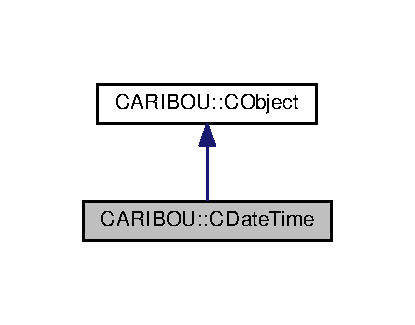
\includegraphics[width=199pt]{class_c_a_r_i_b_o_u_1_1_c_date_time__inherit__graph}
\end{center}
\end{figure}


Collaboration diagram for C\+A\+R\+I\+B\+OU\+:\+:C\+Date\+Time\+:\nopagebreak
\begin{figure}[H]
\begin{center}
\leavevmode
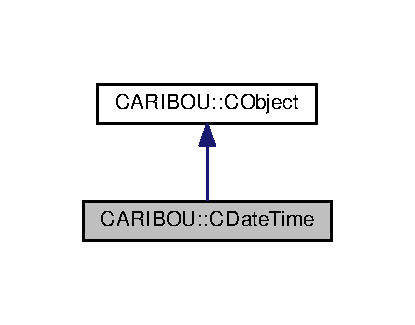
\includegraphics[width=199pt]{class_c_a_r_i_b_o_u_1_1_c_date_time__coll__graph}
\end{center}
\end{figure}
\subsection*{Public Member Functions}
\begin{DoxyCompactItemize}
\item 
{\bf C\+Date\+Time} (bool counter=false)
\item 
{\bf C\+Date\+Time} ({\bf C\+Date\+Time} $\ast$other)
\item 
{\bf C\+Date\+Time} (const {\bf C\+Date\+Time} \&other)
\item 
virtual {\bf $\sim$\+C\+Date\+Time} ()
\item 
virtual void {\bf copy} ({\bf C\+Date\+Time} $\ast$other)
\item 
void {\bf set\+Is\+Counter} (bool b)
\begin{DoxyCompactList}\small\item\em Install or remove a tick listener. \end{DoxyCompactList}\item 
bool {\bf is\+Counter} ()
\item 
void {\bf set\+Ticks} (uint64\+\_\+t {\bf ticks})
\item 
void {\bf set\+Hundredths} (uint8\+\_\+t h)
\item 
void {\bf set\+Tenths} (uint8\+\_\+t {\bf tenths})
\item 
void {\bf set\+Seconds} (uint8\+\_\+t {\bf seconds})
\item 
void {\bf set\+Minutes} (uint8\+\_\+t {\bf minutes})
\item 
void {\bf set\+Hours} (uint8\+\_\+t {\bf hours})
\item 
void {\bf set\+Days} (uint8\+\_\+t {\bf days})
\item 
uint64\+\_\+t {\bf ticks} ()
\item 
uint32\+\_\+t {\bf hundredths} ()
\item 
uint32\+\_\+t {\bf tenths} ()
\item 
uint32\+\_\+t {\bf seconds} ()
\item 
uint32\+\_\+t {\bf minutes} ()
\item 
uint32\+\_\+t {\bf hours} ()
\item 
uint32\+\_\+t {\bf days} ()
\end{DoxyCompactItemize}
\subsection*{Protected Member Functions}
\begin{DoxyCompactItemize}
\item 
virtual void {\bf event} ({\bf C\+Event} $\ast$e)
\begin{DoxyCompactList}\small\item\em receive a queued event, the complement of \doxyref{C\+Object\+::dispatch(\+C\+Event$\ast$)}{p.}{class_c_a_r_i_b_o_u_1_1_c_object_a8aa02620cb58d4e2d3e19999aa0fbfe7}. \end{DoxyCompactList}\item 
void {\bf update} ()
\item 
void {\bf tick} ()
\end{DoxyCompactItemize}
\subsection*{Protected Attributes}
\begin{DoxyCompactItemize}
\item 
caribou\+\_\+timer\+\_\+t $\ast$ {\bf m\+Timer}
\end{DoxyCompactItemize}
\subsection*{Additional Inherited Members}


\subsection{Detailed Description}
Implements a date time object. 

\begin{DoxyAuthor}{Author}
Michael Sharkey {\tt mike@pikeaero.\+com}
\end{DoxyAuthor}
T\+O\+DO
\begin{DoxyItemize}
\item Implement date compare operators
\item Implement date math operators 
\end{DoxyItemize}

Definition at line 34 of file cdatetime.\+h.



\subsection{Constructor \& Destructor Documentation}
\index{C\+A\+R\+I\+B\+O\+U\+::\+C\+Date\+Time@{C\+A\+R\+I\+B\+O\+U\+::\+C\+Date\+Time}!C\+Date\+Time@{C\+Date\+Time}}
\index{C\+Date\+Time@{C\+Date\+Time}!C\+A\+R\+I\+B\+O\+U\+::\+C\+Date\+Time@{C\+A\+R\+I\+B\+O\+U\+::\+C\+Date\+Time}}
\subsubsection[{C\+Date\+Time(bool counter=false)}]{\setlength{\rightskip}{0pt plus 5cm}C\+A\+R\+I\+B\+O\+U\+::\+C\+Date\+Time\+::\+C\+Date\+Time (
\begin{DoxyParamCaption}
\item[{bool}]{counter = {\ttfamily false}}
\end{DoxyParamCaption}
)}\label{class_c_a_r_i_b_o_u_1_1_c_date_time_a3e9a933f943164b46b695a5300141ba2}


Definition at line 35 of file cdatetime.\+cpp.

\index{C\+A\+R\+I\+B\+O\+U\+::\+C\+Date\+Time@{C\+A\+R\+I\+B\+O\+U\+::\+C\+Date\+Time}!C\+Date\+Time@{C\+Date\+Time}}
\index{C\+Date\+Time@{C\+Date\+Time}!C\+A\+R\+I\+B\+O\+U\+::\+C\+Date\+Time@{C\+A\+R\+I\+B\+O\+U\+::\+C\+Date\+Time}}
\subsubsection[{C\+Date\+Time(\+C\+Date\+Time $\ast$other)}]{\setlength{\rightskip}{0pt plus 5cm}C\+A\+R\+I\+B\+O\+U\+::\+C\+Date\+Time\+::\+C\+Date\+Time (
\begin{DoxyParamCaption}
\item[{{\bf C\+Date\+Time} $\ast$}]{other}
\end{DoxyParamCaption}
)}\label{class_c_a_r_i_b_o_u_1_1_c_date_time_ad430ea8858e05477e2886c3768395570}


Definition at line 49 of file cdatetime.\+cpp.

\index{C\+A\+R\+I\+B\+O\+U\+::\+C\+Date\+Time@{C\+A\+R\+I\+B\+O\+U\+::\+C\+Date\+Time}!C\+Date\+Time@{C\+Date\+Time}}
\index{C\+Date\+Time@{C\+Date\+Time}!C\+A\+R\+I\+B\+O\+U\+::\+C\+Date\+Time@{C\+A\+R\+I\+B\+O\+U\+::\+C\+Date\+Time}}
\subsubsection[{C\+Date\+Time(const C\+Date\+Time \&other)}]{\setlength{\rightskip}{0pt plus 5cm}C\+A\+R\+I\+B\+O\+U\+::\+C\+Date\+Time\+::\+C\+Date\+Time (
\begin{DoxyParamCaption}
\item[{const {\bf C\+Date\+Time} \&}]{other}
\end{DoxyParamCaption}
)\hspace{0.3cm}{\ttfamily [inline]}}\label{class_c_a_r_i_b_o_u_1_1_c_date_time_ad30c5f09bc4ff6c37264ef2c4ccf24d9}


Definition at line 39 of file cdatetime.\+h.

\index{C\+A\+R\+I\+B\+O\+U\+::\+C\+Date\+Time@{C\+A\+R\+I\+B\+O\+U\+::\+C\+Date\+Time}!````~C\+Date\+Time@{$\sim$\+C\+Date\+Time}}
\index{````~C\+Date\+Time@{$\sim$\+C\+Date\+Time}!C\+A\+R\+I\+B\+O\+U\+::\+C\+Date\+Time@{C\+A\+R\+I\+B\+O\+U\+::\+C\+Date\+Time}}
\subsubsection[{$\sim$\+C\+Date\+Time()}]{\setlength{\rightskip}{0pt plus 5cm}C\+A\+R\+I\+B\+O\+U\+::\+C\+Date\+Time\+::$\sim$\+C\+Date\+Time (
\begin{DoxyParamCaption}
{}
\end{DoxyParamCaption}
)\hspace{0.3cm}{\ttfamily [virtual]}}\label{class_c_a_r_i_b_o_u_1_1_c_date_time_a248ce9aa1aee4fd0ac64297a42d8b1ad}


Definition at line 55 of file cdatetime.\+cpp.



\subsection{Member Function Documentation}
\index{C\+A\+R\+I\+B\+O\+U\+::\+C\+Date\+Time@{C\+A\+R\+I\+B\+O\+U\+::\+C\+Date\+Time}!copy@{copy}}
\index{copy@{copy}!C\+A\+R\+I\+B\+O\+U\+::\+C\+Date\+Time@{C\+A\+R\+I\+B\+O\+U\+::\+C\+Date\+Time}}
\subsubsection[{copy(\+C\+Date\+Time $\ast$other)}]{\setlength{\rightskip}{0pt plus 5cm}void C\+A\+R\+I\+B\+O\+U\+::\+C\+Date\+Time\+::copy (
\begin{DoxyParamCaption}
\item[{{\bf C\+Date\+Time} $\ast$}]{other}
\end{DoxyParamCaption}
)\hspace{0.3cm}{\ttfamily [virtual]}}\label{class_c_a_r_i_b_o_u_1_1_c_date_time_a906be995214fc3f666000a2fc54643a9}


Definition at line 64 of file cdatetime.\+cpp.

\index{C\+A\+R\+I\+B\+O\+U\+::\+C\+Date\+Time@{C\+A\+R\+I\+B\+O\+U\+::\+C\+Date\+Time}!days@{days}}
\index{days@{days}!C\+A\+R\+I\+B\+O\+U\+::\+C\+Date\+Time@{C\+A\+R\+I\+B\+O\+U\+::\+C\+Date\+Time}}
\subsubsection[{days()}]{\setlength{\rightskip}{0pt plus 5cm}uint32\+\_\+t C\+A\+R\+I\+B\+O\+U\+::\+C\+Date\+Time\+::days (
\begin{DoxyParamCaption}
{}
\end{DoxyParamCaption}
)\hspace{0.3cm}{\ttfamily [inline]}}\label{class_c_a_r_i_b_o_u_1_1_c_date_time_aa2aa1aee8dd86ce408a49021d7f13fd4}


Definition at line 60 of file cdatetime.\+h.

\index{C\+A\+R\+I\+B\+O\+U\+::\+C\+Date\+Time@{C\+A\+R\+I\+B\+O\+U\+::\+C\+Date\+Time}!event@{event}}
\index{event@{event}!C\+A\+R\+I\+B\+O\+U\+::\+C\+Date\+Time@{C\+A\+R\+I\+B\+O\+U\+::\+C\+Date\+Time}}
\subsubsection[{event(\+C\+Event $\ast$e)}]{\setlength{\rightskip}{0pt plus 5cm}void C\+A\+R\+I\+B\+O\+U\+::\+C\+Date\+Time\+::event (
\begin{DoxyParamCaption}
\item[{{\bf C\+Event} $\ast$}]{e}
\end{DoxyParamCaption}
)\hspace{0.3cm}{\ttfamily [protected]}, {\ttfamily [virtual]}}\label{class_c_a_r_i_b_o_u_1_1_c_date_time_a35c1d14db0523c8da5748ca2b8245bed}


receive a queued event, the complement of \doxyref{C\+Object\+::dispatch(\+C\+Event$\ast$)}{p.}{class_c_a_r_i_b_o_u_1_1_c_object_a8aa02620cb58d4e2d3e19999aa0fbfe7}. 

Process Events. 

Reimplemented from {\bf C\+A\+R\+I\+B\+O\+U\+::\+C\+Object} \doxyref{}{p.}{class_c_a_r_i_b_o_u_1_1_c_object_a3e0d51872e9834666d064c716340bbdd}.



Definition at line 129 of file cdatetime.\+cpp.

\index{C\+A\+R\+I\+B\+O\+U\+::\+C\+Date\+Time@{C\+A\+R\+I\+B\+O\+U\+::\+C\+Date\+Time}!hours@{hours}}
\index{hours@{hours}!C\+A\+R\+I\+B\+O\+U\+::\+C\+Date\+Time@{C\+A\+R\+I\+B\+O\+U\+::\+C\+Date\+Time}}
\subsubsection[{hours()}]{\setlength{\rightskip}{0pt plus 5cm}uint32\+\_\+t C\+A\+R\+I\+B\+O\+U\+::\+C\+Date\+Time\+::hours (
\begin{DoxyParamCaption}
{}
\end{DoxyParamCaption}
)\hspace{0.3cm}{\ttfamily [inline]}}\label{class_c_a_r_i_b_o_u_1_1_c_date_time_a5773cdcc8bee21431dd7871f3872bc1c}


Definition at line 59 of file cdatetime.\+h.

\index{C\+A\+R\+I\+B\+O\+U\+::\+C\+Date\+Time@{C\+A\+R\+I\+B\+O\+U\+::\+C\+Date\+Time}!hundredths@{hundredths}}
\index{hundredths@{hundredths}!C\+A\+R\+I\+B\+O\+U\+::\+C\+Date\+Time@{C\+A\+R\+I\+B\+O\+U\+::\+C\+Date\+Time}}
\subsubsection[{hundredths()}]{\setlength{\rightskip}{0pt plus 5cm}uint32\+\_\+t C\+A\+R\+I\+B\+O\+U\+::\+C\+Date\+Time\+::hundredths (
\begin{DoxyParamCaption}
{}
\end{DoxyParamCaption}
)\hspace{0.3cm}{\ttfamily [inline]}}\label{class_c_a_r_i_b_o_u_1_1_c_date_time_a22bec049f784e68470542ce213535dd7}


Definition at line 55 of file cdatetime.\+h.

\index{C\+A\+R\+I\+B\+O\+U\+::\+C\+Date\+Time@{C\+A\+R\+I\+B\+O\+U\+::\+C\+Date\+Time}!is\+Counter@{is\+Counter}}
\index{is\+Counter@{is\+Counter}!C\+A\+R\+I\+B\+O\+U\+::\+C\+Date\+Time@{C\+A\+R\+I\+B\+O\+U\+::\+C\+Date\+Time}}
\subsubsection[{is\+Counter()}]{\setlength{\rightskip}{0pt plus 5cm}bool C\+A\+R\+I\+B\+O\+U\+::\+C\+Date\+Time\+::is\+Counter (
\begin{DoxyParamCaption}
{}
\end{DoxyParamCaption}
)}\label{class_c_a_r_i_b_o_u_1_1_c_date_time_a5b1a1ec998fba3305b3b1c3d9aad0fbc}


Definition at line 93 of file cdatetime.\+cpp.

\index{C\+A\+R\+I\+B\+O\+U\+::\+C\+Date\+Time@{C\+A\+R\+I\+B\+O\+U\+::\+C\+Date\+Time}!minutes@{minutes}}
\index{minutes@{minutes}!C\+A\+R\+I\+B\+O\+U\+::\+C\+Date\+Time@{C\+A\+R\+I\+B\+O\+U\+::\+C\+Date\+Time}}
\subsubsection[{minutes()}]{\setlength{\rightskip}{0pt plus 5cm}uint32\+\_\+t C\+A\+R\+I\+B\+O\+U\+::\+C\+Date\+Time\+::minutes (
\begin{DoxyParamCaption}
{}
\end{DoxyParamCaption}
)\hspace{0.3cm}{\ttfamily [inline]}}\label{class_c_a_r_i_b_o_u_1_1_c_date_time_aff87a55b57a49b3ea31198328b52bea6}


Definition at line 58 of file cdatetime.\+h.

\index{C\+A\+R\+I\+B\+O\+U\+::\+C\+Date\+Time@{C\+A\+R\+I\+B\+O\+U\+::\+C\+Date\+Time}!seconds@{seconds}}
\index{seconds@{seconds}!C\+A\+R\+I\+B\+O\+U\+::\+C\+Date\+Time@{C\+A\+R\+I\+B\+O\+U\+::\+C\+Date\+Time}}
\subsubsection[{seconds()}]{\setlength{\rightskip}{0pt plus 5cm}uint32\+\_\+t C\+A\+R\+I\+B\+O\+U\+::\+C\+Date\+Time\+::seconds (
\begin{DoxyParamCaption}
{}
\end{DoxyParamCaption}
)\hspace{0.3cm}{\ttfamily [inline]}}\label{class_c_a_r_i_b_o_u_1_1_c_date_time_a3254197088aee6e8a6bc48f4145f0d6b}


Definition at line 57 of file cdatetime.\+h.

\index{C\+A\+R\+I\+B\+O\+U\+::\+C\+Date\+Time@{C\+A\+R\+I\+B\+O\+U\+::\+C\+Date\+Time}!set\+Days@{set\+Days}}
\index{set\+Days@{set\+Days}!C\+A\+R\+I\+B\+O\+U\+::\+C\+Date\+Time@{C\+A\+R\+I\+B\+O\+U\+::\+C\+Date\+Time}}
\subsubsection[{set\+Days(uint8\+\_\+t days)}]{\setlength{\rightskip}{0pt plus 5cm}void C\+A\+R\+I\+B\+O\+U\+::\+C\+Date\+Time\+::set\+Days (
\begin{DoxyParamCaption}
\item[{uint8\+\_\+t}]{days}
\end{DoxyParamCaption}
)\hspace{0.3cm}{\ttfamily [inline]}}\label{class_c_a_r_i_b_o_u_1_1_c_date_time_a7fefdb12be77abe2f8014a7b1f642f0d}


Definition at line 52 of file cdatetime.\+h.

\index{C\+A\+R\+I\+B\+O\+U\+::\+C\+Date\+Time@{C\+A\+R\+I\+B\+O\+U\+::\+C\+Date\+Time}!set\+Hours@{set\+Hours}}
\index{set\+Hours@{set\+Hours}!C\+A\+R\+I\+B\+O\+U\+::\+C\+Date\+Time@{C\+A\+R\+I\+B\+O\+U\+::\+C\+Date\+Time}}
\subsubsection[{set\+Hours(uint8\+\_\+t hours)}]{\setlength{\rightskip}{0pt plus 5cm}void C\+A\+R\+I\+B\+O\+U\+::\+C\+Date\+Time\+::set\+Hours (
\begin{DoxyParamCaption}
\item[{uint8\+\_\+t}]{hours}
\end{DoxyParamCaption}
)\hspace{0.3cm}{\ttfamily [inline]}}\label{class_c_a_r_i_b_o_u_1_1_c_date_time_a280e5043c447010d533b9da01f8aac58}


Definition at line 51 of file cdatetime.\+h.

\index{C\+A\+R\+I\+B\+O\+U\+::\+C\+Date\+Time@{C\+A\+R\+I\+B\+O\+U\+::\+C\+Date\+Time}!set\+Hundredths@{set\+Hundredths}}
\index{set\+Hundredths@{set\+Hundredths}!C\+A\+R\+I\+B\+O\+U\+::\+C\+Date\+Time@{C\+A\+R\+I\+B\+O\+U\+::\+C\+Date\+Time}}
\subsubsection[{set\+Hundredths(uint8\+\_\+t h)}]{\setlength{\rightskip}{0pt plus 5cm}void C\+A\+R\+I\+B\+O\+U\+::\+C\+Date\+Time\+::set\+Hundredths (
\begin{DoxyParamCaption}
\item[{uint8\+\_\+t}]{h}
\end{DoxyParamCaption}
)\hspace{0.3cm}{\ttfamily [inline]}}\label{class_c_a_r_i_b_o_u_1_1_c_date_time_a0e2808555dc3b55675590e19fdfbcc2b}


Definition at line 47 of file cdatetime.\+h.

\index{C\+A\+R\+I\+B\+O\+U\+::\+C\+Date\+Time@{C\+A\+R\+I\+B\+O\+U\+::\+C\+Date\+Time}!set\+Is\+Counter@{set\+Is\+Counter}}
\index{set\+Is\+Counter@{set\+Is\+Counter}!C\+A\+R\+I\+B\+O\+U\+::\+C\+Date\+Time@{C\+A\+R\+I\+B\+O\+U\+::\+C\+Date\+Time}}
\subsubsection[{set\+Is\+Counter(bool b)}]{\setlength{\rightskip}{0pt plus 5cm}void C\+A\+R\+I\+B\+O\+U\+::\+C\+Date\+Time\+::set\+Is\+Counter (
\begin{DoxyParamCaption}
\item[{bool}]{b}
\end{DoxyParamCaption}
)}\label{class_c_a_r_i_b_o_u_1_1_c_date_time_a343dc1421c2bc58397a06d0f307a47e4}


Install or remove a tick listener. 



Definition at line 80 of file cdatetime.\+cpp.

\index{C\+A\+R\+I\+B\+O\+U\+::\+C\+Date\+Time@{C\+A\+R\+I\+B\+O\+U\+::\+C\+Date\+Time}!set\+Minutes@{set\+Minutes}}
\index{set\+Minutes@{set\+Minutes}!C\+A\+R\+I\+B\+O\+U\+::\+C\+Date\+Time@{C\+A\+R\+I\+B\+O\+U\+::\+C\+Date\+Time}}
\subsubsection[{set\+Minutes(uint8\+\_\+t minutes)}]{\setlength{\rightskip}{0pt plus 5cm}void C\+A\+R\+I\+B\+O\+U\+::\+C\+Date\+Time\+::set\+Minutes (
\begin{DoxyParamCaption}
\item[{uint8\+\_\+t}]{minutes}
\end{DoxyParamCaption}
)\hspace{0.3cm}{\ttfamily [inline]}}\label{class_c_a_r_i_b_o_u_1_1_c_date_time_aba3ee3c94cf0d2e3183a0f488b6dd033}


Definition at line 50 of file cdatetime.\+h.

\index{C\+A\+R\+I\+B\+O\+U\+::\+C\+Date\+Time@{C\+A\+R\+I\+B\+O\+U\+::\+C\+Date\+Time}!set\+Seconds@{set\+Seconds}}
\index{set\+Seconds@{set\+Seconds}!C\+A\+R\+I\+B\+O\+U\+::\+C\+Date\+Time@{C\+A\+R\+I\+B\+O\+U\+::\+C\+Date\+Time}}
\subsubsection[{set\+Seconds(uint8\+\_\+t seconds)}]{\setlength{\rightskip}{0pt plus 5cm}void C\+A\+R\+I\+B\+O\+U\+::\+C\+Date\+Time\+::set\+Seconds (
\begin{DoxyParamCaption}
\item[{uint8\+\_\+t}]{seconds}
\end{DoxyParamCaption}
)\hspace{0.3cm}{\ttfamily [inline]}}\label{class_c_a_r_i_b_o_u_1_1_c_date_time_aa8593ca4fa1d012fba98d3b9bd8f77d8}


Definition at line 49 of file cdatetime.\+h.

\index{C\+A\+R\+I\+B\+O\+U\+::\+C\+Date\+Time@{C\+A\+R\+I\+B\+O\+U\+::\+C\+Date\+Time}!set\+Tenths@{set\+Tenths}}
\index{set\+Tenths@{set\+Tenths}!C\+A\+R\+I\+B\+O\+U\+::\+C\+Date\+Time@{C\+A\+R\+I\+B\+O\+U\+::\+C\+Date\+Time}}
\subsubsection[{set\+Tenths(uint8\+\_\+t tenths)}]{\setlength{\rightskip}{0pt plus 5cm}void C\+A\+R\+I\+B\+O\+U\+::\+C\+Date\+Time\+::set\+Tenths (
\begin{DoxyParamCaption}
\item[{uint8\+\_\+t}]{tenths}
\end{DoxyParamCaption}
)\hspace{0.3cm}{\ttfamily [inline]}}\label{class_c_a_r_i_b_o_u_1_1_c_date_time_a20353c0d37254bf97f45eb5befe2cd02}


Definition at line 48 of file cdatetime.\+h.

\index{C\+A\+R\+I\+B\+O\+U\+::\+C\+Date\+Time@{C\+A\+R\+I\+B\+O\+U\+::\+C\+Date\+Time}!set\+Ticks@{set\+Ticks}}
\index{set\+Ticks@{set\+Ticks}!C\+A\+R\+I\+B\+O\+U\+::\+C\+Date\+Time@{C\+A\+R\+I\+B\+O\+U\+::\+C\+Date\+Time}}
\subsubsection[{set\+Ticks(uint64\+\_\+t ticks)}]{\setlength{\rightskip}{0pt plus 5cm}void C\+A\+R\+I\+B\+O\+U\+::\+C\+Date\+Time\+::set\+Ticks (
\begin{DoxyParamCaption}
\item[{uint64\+\_\+t}]{ticks}
\end{DoxyParamCaption}
)\hspace{0.3cm}{\ttfamily [inline]}}\label{class_c_a_r_i_b_o_u_1_1_c_date_time_ac850c898febbc1989503570b59f31e5c}


Definition at line 46 of file cdatetime.\+h.

\index{C\+A\+R\+I\+B\+O\+U\+::\+C\+Date\+Time@{C\+A\+R\+I\+B\+O\+U\+::\+C\+Date\+Time}!tenths@{tenths}}
\index{tenths@{tenths}!C\+A\+R\+I\+B\+O\+U\+::\+C\+Date\+Time@{C\+A\+R\+I\+B\+O\+U\+::\+C\+Date\+Time}}
\subsubsection[{tenths()}]{\setlength{\rightskip}{0pt plus 5cm}uint32\+\_\+t C\+A\+R\+I\+B\+O\+U\+::\+C\+Date\+Time\+::tenths (
\begin{DoxyParamCaption}
{}
\end{DoxyParamCaption}
)\hspace{0.3cm}{\ttfamily [inline]}}\label{class_c_a_r_i_b_o_u_1_1_c_date_time_a323016e094c4e7ee9a75ae6b98388f60}


Definition at line 56 of file cdatetime.\+h.

\index{C\+A\+R\+I\+B\+O\+U\+::\+C\+Date\+Time@{C\+A\+R\+I\+B\+O\+U\+::\+C\+Date\+Time}!tick@{tick}}
\index{tick@{tick}!C\+A\+R\+I\+B\+O\+U\+::\+C\+Date\+Time@{C\+A\+R\+I\+B\+O\+U\+::\+C\+Date\+Time}}
\subsubsection[{tick()}]{\setlength{\rightskip}{0pt plus 5cm}void C\+A\+R\+I\+B\+O\+U\+::\+C\+Date\+Time\+::tick (
\begin{DoxyParamCaption}
{}
\end{DoxyParamCaption}
)\hspace{0.3cm}{\ttfamily [protected]}}\label{class_c_a_r_i_b_o_u_1_1_c_date_time_af2b32c1458dbaeade3e4062f387ca06d}


Definition at line 123 of file cdatetime.\+cpp.

\index{C\+A\+R\+I\+B\+O\+U\+::\+C\+Date\+Time@{C\+A\+R\+I\+B\+O\+U\+::\+C\+Date\+Time}!ticks@{ticks}}
\index{ticks@{ticks}!C\+A\+R\+I\+B\+O\+U\+::\+C\+Date\+Time@{C\+A\+R\+I\+B\+O\+U\+::\+C\+Date\+Time}}
\subsubsection[{ticks()}]{\setlength{\rightskip}{0pt plus 5cm}uint64\+\_\+t C\+A\+R\+I\+B\+O\+U\+::\+C\+Date\+Time\+::ticks (
\begin{DoxyParamCaption}
{}
\end{DoxyParamCaption}
)\hspace{0.3cm}{\ttfamily [inline]}}\label{class_c_a_r_i_b_o_u_1_1_c_date_time_a41cbd72922ffe19f74f45fda43fd5fad}


Definition at line 54 of file cdatetime.\+h.

\index{C\+A\+R\+I\+B\+O\+U\+::\+C\+Date\+Time@{C\+A\+R\+I\+B\+O\+U\+::\+C\+Date\+Time}!update@{update}}
\index{update@{update}!C\+A\+R\+I\+B\+O\+U\+::\+C\+Date\+Time@{C\+A\+R\+I\+B\+O\+U\+::\+C\+Date\+Time}}
\subsubsection[{update()}]{\setlength{\rightskip}{0pt plus 5cm}void C\+A\+R\+I\+B\+O\+U\+::\+C\+Date\+Time\+::update (
\begin{DoxyParamCaption}
{}
\end{DoxyParamCaption}
)\hspace{0.3cm}{\ttfamily [protected]}}\label{class_c_a_r_i_b_o_u_1_1_c_date_time_a55bb6fca66abe9bd37ca726b207c8422}


Definition at line 98 of file cdatetime.\+cpp.



\subsection{Member Data Documentation}
\index{C\+A\+R\+I\+B\+O\+U\+::\+C\+Date\+Time@{C\+A\+R\+I\+B\+O\+U\+::\+C\+Date\+Time}!m\+Timer@{m\+Timer}}
\index{m\+Timer@{m\+Timer}!C\+A\+R\+I\+B\+O\+U\+::\+C\+Date\+Time@{C\+A\+R\+I\+B\+O\+U\+::\+C\+Date\+Time}}
\subsubsection[{m\+Timer}]{\setlength{\rightskip}{0pt plus 5cm}caribou\+\_\+timer\+\_\+t$\ast$ C\+A\+R\+I\+B\+O\+U\+::\+C\+Date\+Time\+::m\+Timer\hspace{0.3cm}{\ttfamily [protected]}}\label{class_c_a_r_i_b_o_u_1_1_c_date_time_a31513549e06aa4539ba8d5a179f010ea}


Definition at line 66 of file cdatetime.\+h.



The documentation for this class was generated from the following files\+:\begin{DoxyCompactItemize}
\item 
include/caribou++/{\bf cdatetime.\+h}\item 
src/{\bf cdatetime.\+cpp}\end{DoxyCompactItemize}

\section{C\-A\-R\-I\-B\-O\-U\-:\-:C\-Demo\-Thread Class Reference}
\label{class_c_a_r_i_b_o_u_1_1_c_demo_thread}\index{C\-A\-R\-I\-B\-O\-U\-::\-C\-Demo\-Thread@{C\-A\-R\-I\-B\-O\-U\-::\-C\-Demo\-Thread}}


{\ttfamily \#include $<$caribou++demo.\-h$>$}



Inheritance diagram for C\-A\-R\-I\-B\-O\-U\-:\-:C\-Demo\-Thread\-:\nopagebreak
\begin{figure}[H]
\begin{center}
\leavevmode
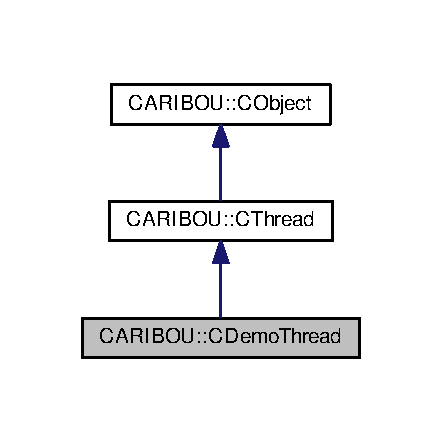
\includegraphics[width=212pt]{class_c_a_r_i_b_o_u_1_1_c_demo_thread__inherit__graph}
\end{center}
\end{figure}


Collaboration diagram for C\-A\-R\-I\-B\-O\-U\-:\-:C\-Demo\-Thread\-:\nopagebreak
\begin{figure}[H]
\begin{center}
\leavevmode
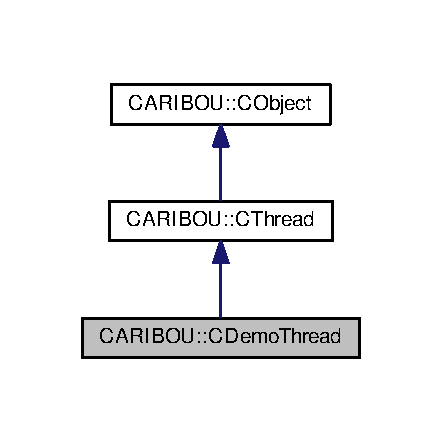
\includegraphics[width=212pt]{class_c_a_r_i_b_o_u_1_1_c_demo_thread__coll__graph}
\end{center}
\end{figure}
\subsection*{Public Member Functions}
\begin{DoxyCompactItemize}
\item 
{\bf C\-Demo\-Thread} (const char $\ast${\bf name}, C\-I\-O\-Device $\ast$device, uint16\-\_\-t stksize=512, uint16\-\_\-t {\bf priority}=N\-O\-R\-M\-A\-L\-P\-R\-I\-O)
\item 
virtual {\bf $\sim$\-C\-Demo\-Thread} ()
\item 
virtual void {\bf run} ()
\end{DoxyCompactItemize}
\subsection*{Protected Member Functions}
\begin{DoxyCompactItemize}
\item 
virtual void {\bf event} ({\bf C\-A\-R\-I\-B\-O\-U\-::\-C\-Event} $\ast$event)
\begin{DoxyCompactList}\small\item\em receive a queued event, the complement of \doxyref{C\-Object\-::dispatch(\-C\-Event$\ast$)}{p.}{class_c_a_r_i_b_o_u_1_1_c_object_a8aa02620cb58d4e2d3e19999aa0fbfe7}. \end{DoxyCompactList}\end{DoxyCompactItemize}
\subsection*{Additional Inherited Members}


\subsection{Detailed Description}


Definition at line 18 of file caribou++demo.\-h.



\subsection{Constructor \& Destructor Documentation}
\index{C\-A\-R\-I\-B\-O\-U\-::\-C\-Demo\-Thread@{C\-A\-R\-I\-B\-O\-U\-::\-C\-Demo\-Thread}!C\-Demo\-Thread@{C\-Demo\-Thread}}
\index{C\-Demo\-Thread@{C\-Demo\-Thread}!CARIBOU::CDemoThread@{C\-A\-R\-I\-B\-O\-U\-::\-C\-Demo\-Thread}}
\subsubsection[{C\-Demo\-Thread}]{\setlength{\rightskip}{0pt plus 5cm}C\-A\-R\-I\-B\-O\-U\-::\-C\-Demo\-Thread\-::\-C\-Demo\-Thread (
\begin{DoxyParamCaption}
\item[{const char $\ast$}]{name, }
\item[{C\-I\-O\-Device $\ast$}]{device, }
\item[{uint16\-\_\-t}]{stksize = {\ttfamily 512}, }
\item[{uint16\-\_\-t}]{priority = {\ttfamily NORMALPRIO}}
\end{DoxyParamCaption}
)}\label{class_c_a_r_i_b_o_u_1_1_c_demo_thread_a9d16297d0e16fc11dadf913e5c633d80}


Definition at line 18 of file caribou++demo.\-cpp.

\index{C\-A\-R\-I\-B\-O\-U\-::\-C\-Demo\-Thread@{C\-A\-R\-I\-B\-O\-U\-::\-C\-Demo\-Thread}!$\sim$\-C\-Demo\-Thread@{$\sim$\-C\-Demo\-Thread}}
\index{$\sim$\-C\-Demo\-Thread@{$\sim$\-C\-Demo\-Thread}!CARIBOU::CDemoThread@{C\-A\-R\-I\-B\-O\-U\-::\-C\-Demo\-Thread}}
\subsubsection[{$\sim$\-C\-Demo\-Thread}]{\setlength{\rightskip}{0pt plus 5cm}C\-A\-R\-I\-B\-O\-U\-::\-C\-Demo\-Thread\-::$\sim$\-C\-Demo\-Thread (
\begin{DoxyParamCaption}
{}
\end{DoxyParamCaption}
)\hspace{0.3cm}{\ttfamily [virtual]}}\label{class_c_a_r_i_b_o_u_1_1_c_demo_thread_aad213cf733ba363d0a075a64a718606c}


Definition at line 29 of file caribou++demo.\-cpp.



\subsection{Member Function Documentation}
\index{C\-A\-R\-I\-B\-O\-U\-::\-C\-Demo\-Thread@{C\-A\-R\-I\-B\-O\-U\-::\-C\-Demo\-Thread}!event@{event}}
\index{event@{event}!CARIBOU::CDemoThread@{C\-A\-R\-I\-B\-O\-U\-::\-C\-Demo\-Thread}}
\subsubsection[{event}]{\setlength{\rightskip}{0pt plus 5cm}void C\-A\-R\-I\-B\-O\-U\-::\-C\-Demo\-Thread\-::event (
\begin{DoxyParamCaption}
\item[{{\bf C\-A\-R\-I\-B\-O\-U\-::\-C\-Event} $\ast$}]{e}
\end{DoxyParamCaption}
)\hspace{0.3cm}{\ttfamily [protected]}, {\ttfamily [virtual]}}\label{class_c_a_r_i_b_o_u_1_1_c_demo_thread_a28c300137fb5433552299575036eddc6}


receive a queued event, the complement of \doxyref{C\-Object\-::dispatch(\-C\-Event$\ast$)}{p.}{class_c_a_r_i_b_o_u_1_1_c_object_a8aa02620cb58d4e2d3e19999aa0fbfe7}. 

Process Events. 

Reimplemented from {\bf C\-A\-R\-I\-B\-O\-U\-::\-C\-Object} \doxyref{}{p.}{class_c_a_r_i_b_o_u_1_1_c_object_a3e0d51872e9834666d064c716340bbdd}.



Definition at line 79 of file caribou++demo.\-cpp.

\index{C\-A\-R\-I\-B\-O\-U\-::\-C\-Demo\-Thread@{C\-A\-R\-I\-B\-O\-U\-::\-C\-Demo\-Thread}!run@{run}}
\index{run@{run}!CARIBOU::CDemoThread@{C\-A\-R\-I\-B\-O\-U\-::\-C\-Demo\-Thread}}
\subsubsection[{run}]{\setlength{\rightskip}{0pt plus 5cm}void C\-A\-R\-I\-B\-O\-U\-::\-C\-Demo\-Thread\-::run (
\begin{DoxyParamCaption}
{}
\end{DoxyParamCaption}
)\hspace{0.3cm}{\ttfamily [virtual]}}\label{class_c_a_r_i_b_o_u_1_1_c_demo_thread_a8d2763e9b70a9ecb17b0da5b8f3d7eb0}


Implements {\bf C\-A\-R\-I\-B\-O\-U\-::\-C\-Thread} \doxyref{}{p.}{class_c_a_r_i_b_o_u_1_1_c_thread_a087ae48a158aca84892aea7f9ed16711}.



Definition at line 36 of file caribou++demo.\-cpp.



The documentation for this class was generated from the following files\-:\begin{DoxyCompactItemize}
\item 
demo/include/{\bf caribou++demo.\-h}\item 
demo/src/{\bf caribou++demo.\-cpp}\end{DoxyCompactItemize}

\section{C\+A\+R\+I\+B\+OU\+:\+:C\+Event Class Reference}
\label{class_c_a_r_i_b_o_u_1_1_c_event}\index{C\+A\+R\+I\+B\+O\+U\+::\+C\+Event@{C\+A\+R\+I\+B\+O\+U\+::\+C\+Event}}


Implements an event object.  




{\ttfamily \#include $<$cevent.\+h$>$}



Inheritance diagram for C\+A\+R\+I\+B\+OU\+:\+:C\+Event\+:\nopagebreak
\begin{figure}[H]
\begin{center}
\leavevmode
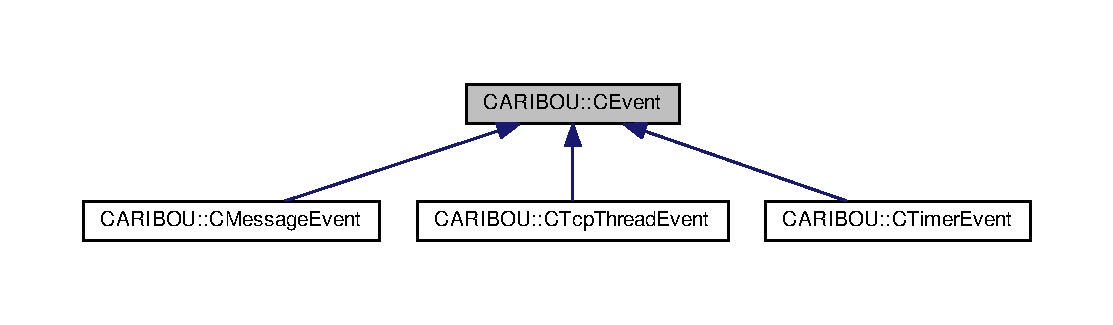
\includegraphics[width=350pt]{class_c_a_r_i_b_o_u_1_1_c_event__inherit__graph}
\end{center}
\end{figure}
\subsection*{Public Types}
\begin{DoxyCompactItemize}
\item 
enum {\bf Type} \{ \\*
{\bf Invalid} = 0, 
{\bf Message\+Event}, 
{\bf Timer\+Event}, 
{\bf User\+Type} = 1000, 
\\*
{\bf Maximum}
 \}
\item 
enum {\bf Priority} \{ {\bf Priority\+Low} =0, 
{\bf Priority\+Standard}, 
{\bf Priority\+High}
 \}
\end{DoxyCompactItemize}
\subsection*{Public Member Functions}
\begin{DoxyCompactItemize}
\item 
{\bf C\+Event} ({\bf C\+Object} $\ast${\bf sender}={\bf N\+U\+LL}, bool {\bf sender\+Owns}=false, {\bf C\+Object} $\ast${\bf receiver}={\bf N\+U\+LL})
\item 
{\bf C\+Event} (const {\bf C\+Event} \&other)
\item 
{\bf C\+Event} ({\bf C\+Event} $\ast$other)
\item 
virtual {\bf $\sim$\+C\+Event} ()
\item 
virtual void {\bf copy} (const {\bf C\+Event} \&other)
\item 
virtual void {\bf set\+Priority} ({\bf Priority} p)
\item 
virtual {\bf Priority} {\bf priority} ()
\item 
virtual void {\bf set\+Type} ({\bf Type} {\bf type})
\item 
virtual {\bf Type} {\bf type} ()
\item 
virtual void {\bf set\+Sender} ({\bf C\+Object} $\ast$object)
\item 
virtual {\bf C\+Object} $\ast$ {\bf sender} ()
\item 
virtual void {\bf set\+Receiver} ({\bf C\+Object} $\ast$object)
\item 
virtual {\bf C\+Object} $\ast$ {\bf receiver} ()
\item 
void {\bf set\+Sender\+Owns} (bool {\bf sender\+Owns})
\begin{DoxyCompactList}\small\item\em Sender-\/ownership of the event is only allowed when using callback dispatch, not to be used with C\+Event\+Queue dispatch! \end{DoxyCompactList}\item 
bool {\bf sender\+Owns} ()
\end{DoxyCompactItemize}


\subsection{Detailed Description}
Implements an event object. 

\begin{DoxyAuthor}{Author}
Michael Sharkey {\tt mike@pikeaero.\+com} 
\end{DoxyAuthor}


Definition at line 29 of file cevent.\+h.



\subsection{Member Enumeration Documentation}
\index{C\+A\+R\+I\+B\+O\+U\+::\+C\+Event@{C\+A\+R\+I\+B\+O\+U\+::\+C\+Event}!Priority@{Priority}}
\index{Priority@{Priority}!C\+A\+R\+I\+B\+O\+U\+::\+C\+Event@{C\+A\+R\+I\+B\+O\+U\+::\+C\+Event}}
\subsubsection[{Priority}]{\setlength{\rightskip}{0pt plus 5cm}enum {\bf C\+A\+R\+I\+B\+O\+U\+::\+C\+Event\+::\+Priority}}\label{class_c_a_r_i_b_o_u_1_1_c_event_a17c4479bfd0ca923739f8602ac4669ac}
\begin{Desc}
\item[Enumerator]\par
\begin{description}
\index{Priority\+Low@{Priority\+Low}!C\+A\+R\+I\+B\+O\+U\+::\+C\+Event@{C\+A\+R\+I\+B\+O\+U\+::\+C\+Event}}\index{C\+A\+R\+I\+B\+O\+U\+::\+C\+Event@{C\+A\+R\+I\+B\+O\+U\+::\+C\+Event}!Priority\+Low@{Priority\+Low}}\item[{\em 
Priority\+Low\label{class_c_a_r_i_b_o_u_1_1_c_event_a17c4479bfd0ca923739f8602ac4669acaa8bdd8f8a6b61b92dd97cb8e5f3d3a00}
}]\index{Priority\+Standard@{Priority\+Standard}!C\+A\+R\+I\+B\+O\+U\+::\+C\+Event@{C\+A\+R\+I\+B\+O\+U\+::\+C\+Event}}\index{C\+A\+R\+I\+B\+O\+U\+::\+C\+Event@{C\+A\+R\+I\+B\+O\+U\+::\+C\+Event}!Priority\+Standard@{Priority\+Standard}}\item[{\em 
Priority\+Standard\label{class_c_a_r_i_b_o_u_1_1_c_event_a17c4479bfd0ca923739f8602ac4669acaaa57d54a5fc40db0ab348c3370b58773}
}]\index{Priority\+High@{Priority\+High}!C\+A\+R\+I\+B\+O\+U\+::\+C\+Event@{C\+A\+R\+I\+B\+O\+U\+::\+C\+Event}}\index{C\+A\+R\+I\+B\+O\+U\+::\+C\+Event@{C\+A\+R\+I\+B\+O\+U\+::\+C\+Event}!Priority\+High@{Priority\+High}}\item[{\em 
Priority\+High\label{class_c_a_r_i_b_o_u_1_1_c_event_a17c4479bfd0ca923739f8602ac4669aca2ec4adefeb94d6fd53a93a7b32cea560}
}]\end{description}
\end{Desc}


Definition at line 39 of file cevent.\+h.

\index{C\+A\+R\+I\+B\+O\+U\+::\+C\+Event@{C\+A\+R\+I\+B\+O\+U\+::\+C\+Event}!Type@{Type}}
\index{Type@{Type}!C\+A\+R\+I\+B\+O\+U\+::\+C\+Event@{C\+A\+R\+I\+B\+O\+U\+::\+C\+Event}}
\subsubsection[{Type}]{\setlength{\rightskip}{0pt plus 5cm}enum {\bf C\+A\+R\+I\+B\+O\+U\+::\+C\+Event\+::\+Type}}\label{class_c_a_r_i_b_o_u_1_1_c_event_a9631f16ad58097aae4e87ca08579cadb}
\begin{Desc}
\item[Enumerator]\par
\begin{description}
\index{Invalid@{Invalid}!C\+A\+R\+I\+B\+O\+U\+::\+C\+Event@{C\+A\+R\+I\+B\+O\+U\+::\+C\+Event}}\index{C\+A\+R\+I\+B\+O\+U\+::\+C\+Event@{C\+A\+R\+I\+B\+O\+U\+::\+C\+Event}!Invalid@{Invalid}}\item[{\em 
Invalid\label{class_c_a_r_i_b_o_u_1_1_c_event_a9631f16ad58097aae4e87ca08579cadba1a931d79d23d27266e6b9eff1ace437c}
}]\index{Message\+Event@{Message\+Event}!C\+A\+R\+I\+B\+O\+U\+::\+C\+Event@{C\+A\+R\+I\+B\+O\+U\+::\+C\+Event}}\index{C\+A\+R\+I\+B\+O\+U\+::\+C\+Event@{C\+A\+R\+I\+B\+O\+U\+::\+C\+Event}!Message\+Event@{Message\+Event}}\item[{\em 
Message\+Event\label{class_c_a_r_i_b_o_u_1_1_c_event_a9631f16ad58097aae4e87ca08579cadba13c359071b6849edc0995c9e1175ca00}
}]\index{Timer\+Event@{Timer\+Event}!C\+A\+R\+I\+B\+O\+U\+::\+C\+Event@{C\+A\+R\+I\+B\+O\+U\+::\+C\+Event}}\index{C\+A\+R\+I\+B\+O\+U\+::\+C\+Event@{C\+A\+R\+I\+B\+O\+U\+::\+C\+Event}!Timer\+Event@{Timer\+Event}}\item[{\em 
Timer\+Event\label{class_c_a_r_i_b_o_u_1_1_c_event_a9631f16ad58097aae4e87ca08579cadba45b8caa4ca6211a239205fc67e4c04b0}
}]\index{User\+Type@{User\+Type}!C\+A\+R\+I\+B\+O\+U\+::\+C\+Event@{C\+A\+R\+I\+B\+O\+U\+::\+C\+Event}}\index{C\+A\+R\+I\+B\+O\+U\+::\+C\+Event@{C\+A\+R\+I\+B\+O\+U\+::\+C\+Event}!User\+Type@{User\+Type}}\item[{\em 
User\+Type\label{class_c_a_r_i_b_o_u_1_1_c_event_a9631f16ad58097aae4e87ca08579cadbaaf2c2b9706305fdc8f728df69b76154b}
}]\index{Maximum@{Maximum}!C\+A\+R\+I\+B\+O\+U\+::\+C\+Event@{C\+A\+R\+I\+B\+O\+U\+::\+C\+Event}}\index{C\+A\+R\+I\+B\+O\+U\+::\+C\+Event@{C\+A\+R\+I\+B\+O\+U\+::\+C\+Event}!Maximum@{Maximum}}\item[{\em 
Maximum\label{class_c_a_r_i_b_o_u_1_1_c_event_a9631f16ad58097aae4e87ca08579cadba9a64ec7d2188dc7f9677f3323ae7d4de}
}]\end{description}
\end{Desc}


Definition at line 32 of file cevent.\+h.



\subsection{Constructor \& Destructor Documentation}
\index{C\+A\+R\+I\+B\+O\+U\+::\+C\+Event@{C\+A\+R\+I\+B\+O\+U\+::\+C\+Event}!C\+Event@{C\+Event}}
\index{C\+Event@{C\+Event}!C\+A\+R\+I\+B\+O\+U\+::\+C\+Event@{C\+A\+R\+I\+B\+O\+U\+::\+C\+Event}}
\subsubsection[{C\+Event(\+C\+Object $\ast$sender=\+N\+U\+L\+L, bool sender\+Owns=false, C\+Object $\ast$receiver=\+N\+U\+L\+L)}]{\setlength{\rightskip}{0pt plus 5cm}C\+A\+R\+I\+B\+O\+U\+::\+C\+Event\+::\+C\+Event (
\begin{DoxyParamCaption}
\item[{{\bf C\+Object} $\ast$}]{sender = {\ttfamily {\bf N\+U\+LL}}, }
\item[{bool}]{sender\+Owns = {\ttfamily false}, }
\item[{{\bf C\+Object} $\ast$}]{receiver = {\ttfamily {\bf N\+U\+LL}}}
\end{DoxyParamCaption}
)}\label{class_c_a_r_i_b_o_u_1_1_c_event_ad9634138e07d4fe856d114a2ddce554c}


Definition at line 22 of file cevent.\+cpp.

\index{C\+A\+R\+I\+B\+O\+U\+::\+C\+Event@{C\+A\+R\+I\+B\+O\+U\+::\+C\+Event}!C\+Event@{C\+Event}}
\index{C\+Event@{C\+Event}!C\+A\+R\+I\+B\+O\+U\+::\+C\+Event@{C\+A\+R\+I\+B\+O\+U\+::\+C\+Event}}
\subsubsection[{C\+Event(const C\+Event \&other)}]{\setlength{\rightskip}{0pt plus 5cm}C\+A\+R\+I\+B\+O\+U\+::\+C\+Event\+::\+C\+Event (
\begin{DoxyParamCaption}
\item[{const {\bf C\+Event} \&}]{other}
\end{DoxyParamCaption}
)\hspace{0.3cm}{\ttfamily [inline]}}\label{class_c_a_r_i_b_o_u_1_1_c_event_a2fc30aa6bb32b006008b8dcf315baa43}


Definition at line 46 of file cevent.\+h.

\index{C\+A\+R\+I\+B\+O\+U\+::\+C\+Event@{C\+A\+R\+I\+B\+O\+U\+::\+C\+Event}!C\+Event@{C\+Event}}
\index{C\+Event@{C\+Event}!C\+A\+R\+I\+B\+O\+U\+::\+C\+Event@{C\+A\+R\+I\+B\+O\+U\+::\+C\+Event}}
\subsubsection[{C\+Event(\+C\+Event $\ast$other)}]{\setlength{\rightskip}{0pt plus 5cm}C\+A\+R\+I\+B\+O\+U\+::\+C\+Event\+::\+C\+Event (
\begin{DoxyParamCaption}
\item[{{\bf C\+Event} $\ast$}]{other}
\end{DoxyParamCaption}
)\hspace{0.3cm}{\ttfamily [inline]}}\label{class_c_a_r_i_b_o_u_1_1_c_event_a68c1c8e496aaa99675a96df91e8e0220}


Definition at line 47 of file cevent.\+h.

\index{C\+A\+R\+I\+B\+O\+U\+::\+C\+Event@{C\+A\+R\+I\+B\+O\+U\+::\+C\+Event}!````~C\+Event@{$\sim$\+C\+Event}}
\index{````~C\+Event@{$\sim$\+C\+Event}!C\+A\+R\+I\+B\+O\+U\+::\+C\+Event@{C\+A\+R\+I\+B\+O\+U\+::\+C\+Event}}
\subsubsection[{$\sim$\+C\+Event()}]{\setlength{\rightskip}{0pt plus 5cm}C\+A\+R\+I\+B\+O\+U\+::\+C\+Event\+::$\sim$\+C\+Event (
\begin{DoxyParamCaption}
{}
\end{DoxyParamCaption}
)\hspace{0.3cm}{\ttfamily [virtual]}}\label{class_c_a_r_i_b_o_u_1_1_c_event_ad0261ddf922300eb4d35fde5894f1d71}


Definition at line 31 of file cevent.\+cpp.



\subsection{Member Function Documentation}
\index{C\+A\+R\+I\+B\+O\+U\+::\+C\+Event@{C\+A\+R\+I\+B\+O\+U\+::\+C\+Event}!copy@{copy}}
\index{copy@{copy}!C\+A\+R\+I\+B\+O\+U\+::\+C\+Event@{C\+A\+R\+I\+B\+O\+U\+::\+C\+Event}}
\subsubsection[{copy(const C\+Event \&other)}]{\setlength{\rightskip}{0pt plus 5cm}void C\+A\+R\+I\+B\+O\+U\+::\+C\+Event\+::copy (
\begin{DoxyParamCaption}
\item[{const {\bf C\+Event} \&}]{other}
\end{DoxyParamCaption}
)\hspace{0.3cm}{\ttfamily [virtual]}}\label{class_c_a_r_i_b_o_u_1_1_c_event_acba684878560c7bec9a4c97f2de4b8c8}


Definition at line 35 of file cevent.\+cpp.

\index{C\+A\+R\+I\+B\+O\+U\+::\+C\+Event@{C\+A\+R\+I\+B\+O\+U\+::\+C\+Event}!priority@{priority}}
\index{priority@{priority}!C\+A\+R\+I\+B\+O\+U\+::\+C\+Event@{C\+A\+R\+I\+B\+O\+U\+::\+C\+Event}}
\subsubsection[{priority()}]{\setlength{\rightskip}{0pt plus 5cm}virtual {\bf Priority} C\+A\+R\+I\+B\+O\+U\+::\+C\+Event\+::priority (
\begin{DoxyParamCaption}
{}
\end{DoxyParamCaption}
)\hspace{0.3cm}{\ttfamily [inline]}, {\ttfamily [virtual]}}\label{class_c_a_r_i_b_o_u_1_1_c_event_a8a0f9460d3a5d5fb1815093692a6bf07}


Definition at line 53 of file cevent.\+h.

\index{C\+A\+R\+I\+B\+O\+U\+::\+C\+Event@{C\+A\+R\+I\+B\+O\+U\+::\+C\+Event}!receiver@{receiver}}
\index{receiver@{receiver}!C\+A\+R\+I\+B\+O\+U\+::\+C\+Event@{C\+A\+R\+I\+B\+O\+U\+::\+C\+Event}}
\subsubsection[{receiver()}]{\setlength{\rightskip}{0pt plus 5cm}virtual {\bf C\+Object}$\ast$ C\+A\+R\+I\+B\+O\+U\+::\+C\+Event\+::receiver (
\begin{DoxyParamCaption}
{}
\end{DoxyParamCaption}
)\hspace{0.3cm}{\ttfamily [inline]}, {\ttfamily [virtual]}}\label{class_c_a_r_i_b_o_u_1_1_c_event_aa712e885d2225da1605bb30cb225ccdf}


Definition at line 62 of file cevent.\+h.

\index{C\+A\+R\+I\+B\+O\+U\+::\+C\+Event@{C\+A\+R\+I\+B\+O\+U\+::\+C\+Event}!sender@{sender}}
\index{sender@{sender}!C\+A\+R\+I\+B\+O\+U\+::\+C\+Event@{C\+A\+R\+I\+B\+O\+U\+::\+C\+Event}}
\subsubsection[{sender()}]{\setlength{\rightskip}{0pt plus 5cm}virtual {\bf C\+Object}$\ast$ C\+A\+R\+I\+B\+O\+U\+::\+C\+Event\+::sender (
\begin{DoxyParamCaption}
{}
\end{DoxyParamCaption}
)\hspace{0.3cm}{\ttfamily [inline]}, {\ttfamily [virtual]}}\label{class_c_a_r_i_b_o_u_1_1_c_event_a142c3eec0ac86c8d26b57e734b6bee83}


Definition at line 59 of file cevent.\+h.

\index{C\+A\+R\+I\+B\+O\+U\+::\+C\+Event@{C\+A\+R\+I\+B\+O\+U\+::\+C\+Event}!sender\+Owns@{sender\+Owns}}
\index{sender\+Owns@{sender\+Owns}!C\+A\+R\+I\+B\+O\+U\+::\+C\+Event@{C\+A\+R\+I\+B\+O\+U\+::\+C\+Event}}
\subsubsection[{sender\+Owns()}]{\setlength{\rightskip}{0pt plus 5cm}bool C\+A\+R\+I\+B\+O\+U\+::\+C\+Event\+::sender\+Owns (
\begin{DoxyParamCaption}
{}
\end{DoxyParamCaption}
)\hspace{0.3cm}{\ttfamily [inline]}}\label{class_c_a_r_i_b_o_u_1_1_c_event_aab86384cb9d3c8fcc4dcf833947f77fb}


Definition at line 66 of file cevent.\+h.

\index{C\+A\+R\+I\+B\+O\+U\+::\+C\+Event@{C\+A\+R\+I\+B\+O\+U\+::\+C\+Event}!set\+Priority@{set\+Priority}}
\index{set\+Priority@{set\+Priority}!C\+A\+R\+I\+B\+O\+U\+::\+C\+Event@{C\+A\+R\+I\+B\+O\+U\+::\+C\+Event}}
\subsubsection[{set\+Priority(\+Priority p)}]{\setlength{\rightskip}{0pt plus 5cm}virtual void C\+A\+R\+I\+B\+O\+U\+::\+C\+Event\+::set\+Priority (
\begin{DoxyParamCaption}
\item[{{\bf Priority}}]{p}
\end{DoxyParamCaption}
)\hspace{0.3cm}{\ttfamily [inline]}, {\ttfamily [virtual]}}\label{class_c_a_r_i_b_o_u_1_1_c_event_a611f81c1dce586793ce3dff3a74474d7}


Definition at line 52 of file cevent.\+h.

\index{C\+A\+R\+I\+B\+O\+U\+::\+C\+Event@{C\+A\+R\+I\+B\+O\+U\+::\+C\+Event}!set\+Receiver@{set\+Receiver}}
\index{set\+Receiver@{set\+Receiver}!C\+A\+R\+I\+B\+O\+U\+::\+C\+Event@{C\+A\+R\+I\+B\+O\+U\+::\+C\+Event}}
\subsubsection[{set\+Receiver(\+C\+Object $\ast$object)}]{\setlength{\rightskip}{0pt plus 5cm}virtual void C\+A\+R\+I\+B\+O\+U\+::\+C\+Event\+::set\+Receiver (
\begin{DoxyParamCaption}
\item[{{\bf C\+Object} $\ast$}]{object}
\end{DoxyParamCaption}
)\hspace{0.3cm}{\ttfamily [inline]}, {\ttfamily [virtual]}}\label{class_c_a_r_i_b_o_u_1_1_c_event_a77714ff356fc6d0595e02174a249ba62}


Definition at line 61 of file cevent.\+h.

\index{C\+A\+R\+I\+B\+O\+U\+::\+C\+Event@{C\+A\+R\+I\+B\+O\+U\+::\+C\+Event}!set\+Sender@{set\+Sender}}
\index{set\+Sender@{set\+Sender}!C\+A\+R\+I\+B\+O\+U\+::\+C\+Event@{C\+A\+R\+I\+B\+O\+U\+::\+C\+Event}}
\subsubsection[{set\+Sender(\+C\+Object $\ast$object)}]{\setlength{\rightskip}{0pt plus 5cm}virtual void C\+A\+R\+I\+B\+O\+U\+::\+C\+Event\+::set\+Sender (
\begin{DoxyParamCaption}
\item[{{\bf C\+Object} $\ast$}]{object}
\end{DoxyParamCaption}
)\hspace{0.3cm}{\ttfamily [inline]}, {\ttfamily [virtual]}}\label{class_c_a_r_i_b_o_u_1_1_c_event_afd5655a5ed5ff952d8219154859619ef}


Definition at line 58 of file cevent.\+h.

\index{C\+A\+R\+I\+B\+O\+U\+::\+C\+Event@{C\+A\+R\+I\+B\+O\+U\+::\+C\+Event}!set\+Sender\+Owns@{set\+Sender\+Owns}}
\index{set\+Sender\+Owns@{set\+Sender\+Owns}!C\+A\+R\+I\+B\+O\+U\+::\+C\+Event@{C\+A\+R\+I\+B\+O\+U\+::\+C\+Event}}
\subsubsection[{set\+Sender\+Owns(bool sender\+Owns)}]{\setlength{\rightskip}{0pt plus 5cm}void C\+A\+R\+I\+B\+O\+U\+::\+C\+Event\+::set\+Sender\+Owns (
\begin{DoxyParamCaption}
\item[{bool}]{sender\+Owns}
\end{DoxyParamCaption}
)\hspace{0.3cm}{\ttfamily [inline]}}\label{class_c_a_r_i_b_o_u_1_1_c_event_ad855b8d97abee8b500c9363e37c067ff}


Sender-\/ownership of the event is only allowed when using callback dispatch, not to be used with C\+Event\+Queue dispatch! 



Definition at line 65 of file cevent.\+h.

\index{C\+A\+R\+I\+B\+O\+U\+::\+C\+Event@{C\+A\+R\+I\+B\+O\+U\+::\+C\+Event}!set\+Type@{set\+Type}}
\index{set\+Type@{set\+Type}!C\+A\+R\+I\+B\+O\+U\+::\+C\+Event@{C\+A\+R\+I\+B\+O\+U\+::\+C\+Event}}
\subsubsection[{set\+Type(\+Type type)}]{\setlength{\rightskip}{0pt plus 5cm}virtual void C\+A\+R\+I\+B\+O\+U\+::\+C\+Event\+::set\+Type (
\begin{DoxyParamCaption}
\item[{{\bf Type}}]{type}
\end{DoxyParamCaption}
)\hspace{0.3cm}{\ttfamily [inline]}, {\ttfamily [virtual]}}\label{class_c_a_r_i_b_o_u_1_1_c_event_affe7d0588719ddbc4d9c99f60145031c}


Definition at line 55 of file cevent.\+h.

\index{C\+A\+R\+I\+B\+O\+U\+::\+C\+Event@{C\+A\+R\+I\+B\+O\+U\+::\+C\+Event}!type@{type}}
\index{type@{type}!C\+A\+R\+I\+B\+O\+U\+::\+C\+Event@{C\+A\+R\+I\+B\+O\+U\+::\+C\+Event}}
\subsubsection[{type()}]{\setlength{\rightskip}{0pt plus 5cm}virtual {\bf Type} C\+A\+R\+I\+B\+O\+U\+::\+C\+Event\+::type (
\begin{DoxyParamCaption}
{}
\end{DoxyParamCaption}
)\hspace{0.3cm}{\ttfamily [inline]}, {\ttfamily [virtual]}}\label{class_c_a_r_i_b_o_u_1_1_c_event_a8772875a6ce54a394f2b020d5167e08c}


Definition at line 56 of file cevent.\+h.



The documentation for this class was generated from the following files\+:\begin{DoxyCompactItemize}
\item 
include/caribou++/{\bf cevent.\+h}\item 
src/{\bf cevent.\+cpp}\end{DoxyCompactItemize}

\section{C\+A\+R\+I\+B\+OU\+:\+:C\+File Class Reference}
\label{class_c_a_r_i_b_o_u_1_1_c_file}\index{C\+A\+R\+I\+B\+O\+U\+::\+C\+File@{C\+A\+R\+I\+B\+O\+U\+::\+C\+File}}


{\ttfamily \#include $<$cfile.\+h$>$}



Inheritance diagram for C\+A\+R\+I\+B\+OU\+:\+:C\+File\+:\nopagebreak
\begin{figure}[H]
\begin{center}
\leavevmode
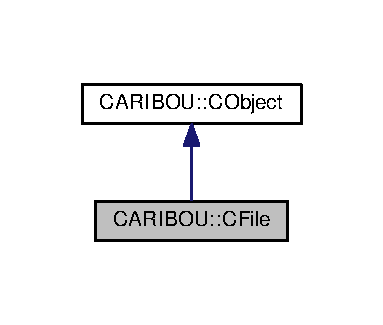
\includegraphics[width=185pt]{class_c_a_r_i_b_o_u_1_1_c_file__inherit__graph}
\end{center}
\end{figure}


Collaboration diagram for C\+A\+R\+I\+B\+OU\+:\+:C\+File\+:\nopagebreak
\begin{figure}[H]
\begin{center}
\leavevmode
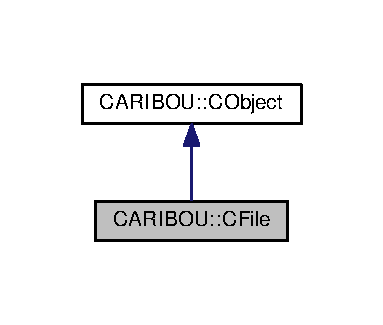
\includegraphics[width=185pt]{class_c_a_r_i_b_o_u_1_1_c_file__coll__graph}
\end{center}
\end{figure}
\subsection*{Public Member Functions}
\begin{DoxyCompactItemize}
\item 
{\bf C\+File} ()
\item 
{\bf C\+File} ({\bf C\+String} {\bf path})
\item 
virtual {\bf $\sim$\+C\+File} ()
\item 
F\+R\+E\+S\+U\+LT {\bf stat} (F\+I\+L\+I\+N\+FO $\ast$info)
\begin{DoxyCompactList}\small\item\em The f\+\_\+stat() function checks the existence of a file or sub-\/directory. \end{DoxyCompactList}\item 
bool {\bf is\+File} ()
\item 
bool {\bf is\+Dir} ()
\item 
bool {\bf mk\+Dir} ()
\begin{DoxyCompactList}\small\item\em Make a directory. \end{DoxyCompactList}\item 
bool {\bf rm\+Dir} ()
\begin{DoxyCompactList}\small\item\em Remove a directory. \end{DoxyCompactList}\item 
void {\bf set\+Path} ({\bf C\+String} {\bf path})
\item 
{\bf C\+A\+R\+I\+B\+O\+U\+::\+C\+String} {\bf path} ()
\item 
{\bf C\+A\+R\+I\+B\+O\+U\+::\+C\+String} {\bf file\+Name} ()
\item 
{\bf C\+A\+R\+I\+B\+O\+U\+::\+C\+String} {\bf file\+Path} ()
\item 
bool {\bf open} (uint8\+\_\+t mode)
\item 
bool {\bf open} ({\bf C\+String} {\bf path}, uint8\+\_\+t mode)
\item 
bool {\bf is\+Open} ()
\item 
void {\bf close} ()
\item 
int {\bf read} (void $\ast$buf, int sz)
\item 
int {\bf read} ({\bf C\+A\+R\+I\+B\+O\+U\+::\+C\+Byte\+Array} \&buf, int sz)
\item 
int {\bf readline} ({\bf C\+A\+R\+I\+B\+O\+U\+::\+C\+Byte\+Array} \&buf, int max)
\begin{DoxyCompactList}\small\item\em Read a line of text from the file. \end{DoxyCompactList}\item 
int {\bf write} (void $\ast$buf, int sz)
\item 
int {\bf write} ({\bf C\+A\+R\+I\+B\+O\+U\+::\+C\+Byte\+Array} \&buf)
\item 
int {\bf seek} (int pos)
\item 
int {\bf tell} ()
\item 
int {\bf size} ()
\item 
bool {\bf eof} ()
\item 
void {\bf sync} ()
\item 
void {\bf truncate} ()
\item 
bool {\bf unlink} ()
\end{DoxyCompactItemize}
\subsection*{Static Public Member Functions}
\begin{DoxyCompactItemize}
\item 
static bool {\bf initialize} (int volume)
\begin{DoxyCompactList}\small\item\em F\+I\+X\+ME -\/ actual support for multiple volumes. \end{DoxyCompactList}\item 
static bool {\bf initialized} ()
\item 
static void {\bf deinitialize} (int volume)
\item 
static F\+A\+T\+FS $\ast$ {\bf fs} ()
\item 
static {\bf C\+A\+R\+I\+B\+O\+U\+::\+C\+String} {\bf md5} ({\bf C\+A\+R\+I\+B\+O\+U\+::\+C\+String} {\bf file\+Path})
\item 
static {\bf C\+A\+R\+I\+B\+O\+U\+::\+C\+String} {\bf temp\+Name} ({\bf C\+A\+R\+I\+B\+O\+U\+::\+C\+String} dir)
\end{DoxyCompactItemize}
\subsection*{Protected Member Functions}
\begin{DoxyCompactItemize}
\item 
void {\bf failure\+Notify} (uint8\+\_\+t err)
\end{DoxyCompactItemize}
\subsection*{Additional Inherited Members}


\subsection{Detailed Description}


Definition at line 30 of file cfile.\+h.



\subsection{Constructor \& Destructor Documentation}
\index{C\+A\+R\+I\+B\+O\+U\+::\+C\+File@{C\+A\+R\+I\+B\+O\+U\+::\+C\+File}!C\+File@{C\+File}}
\index{C\+File@{C\+File}!C\+A\+R\+I\+B\+O\+U\+::\+C\+File@{C\+A\+R\+I\+B\+O\+U\+::\+C\+File}}
\subsubsection[{C\+File()}]{\setlength{\rightskip}{0pt plus 5cm}C\+A\+R\+I\+B\+O\+U\+::\+C\+File\+::\+C\+File (
\begin{DoxyParamCaption}
{}
\end{DoxyParamCaption}
)}\label{class_c_a_r_i_b_o_u_1_1_c_file_aeb88e1a3d5b8c9cd006c2bd552ff12a9}


Definition at line 28 of file cfile.\+cpp.

\index{C\+A\+R\+I\+B\+O\+U\+::\+C\+File@{C\+A\+R\+I\+B\+O\+U\+::\+C\+File}!C\+File@{C\+File}}
\index{C\+File@{C\+File}!C\+A\+R\+I\+B\+O\+U\+::\+C\+File@{C\+A\+R\+I\+B\+O\+U\+::\+C\+File}}
\subsubsection[{C\+File(\+C\+String path)}]{\setlength{\rightskip}{0pt plus 5cm}C\+A\+R\+I\+B\+O\+U\+::\+C\+File\+::\+C\+File (
\begin{DoxyParamCaption}
\item[{{\bf C\+String}}]{path}
\end{DoxyParamCaption}
)}\label{class_c_a_r_i_b_o_u_1_1_c_file_a6d5b3fc0810f3f0b80b658391611caf3}


Definition at line 35 of file cfile.\+cpp.

\index{C\+A\+R\+I\+B\+O\+U\+::\+C\+File@{C\+A\+R\+I\+B\+O\+U\+::\+C\+File}!````~C\+File@{$\sim$\+C\+File}}
\index{````~C\+File@{$\sim$\+C\+File}!C\+A\+R\+I\+B\+O\+U\+::\+C\+File@{C\+A\+R\+I\+B\+O\+U\+::\+C\+File}}
\subsubsection[{$\sim$\+C\+File()}]{\setlength{\rightskip}{0pt plus 5cm}C\+A\+R\+I\+B\+O\+U\+::\+C\+File\+::$\sim$\+C\+File (
\begin{DoxyParamCaption}
{}
\end{DoxyParamCaption}
)\hspace{0.3cm}{\ttfamily [virtual]}}\label{class_c_a_r_i_b_o_u_1_1_c_file_aef0245b264a0c60ec2605b52f9fe7b99}


Definition at line 43 of file cfile.\+cpp.



\subsection{Member Function Documentation}
\index{C\+A\+R\+I\+B\+O\+U\+::\+C\+File@{C\+A\+R\+I\+B\+O\+U\+::\+C\+File}!close@{close}}
\index{close@{close}!C\+A\+R\+I\+B\+O\+U\+::\+C\+File@{C\+A\+R\+I\+B\+O\+U\+::\+C\+File}}
\subsubsection[{close()}]{\setlength{\rightskip}{0pt plus 5cm}void C\+A\+R\+I\+B\+O\+U\+::\+C\+File\+::close (
\begin{DoxyParamCaption}
{}
\end{DoxyParamCaption}
)}\label{class_c_a_r_i_b_o_u_1_1_c_file_a3cc4fea3ed9029fd3bfb2ba8afc8d25c}


Definition at line 240 of file cfile.\+cpp.

\index{C\+A\+R\+I\+B\+O\+U\+::\+C\+File@{C\+A\+R\+I\+B\+O\+U\+::\+C\+File}!deinitialize@{deinitialize}}
\index{deinitialize@{deinitialize}!C\+A\+R\+I\+B\+O\+U\+::\+C\+File@{C\+A\+R\+I\+B\+O\+U\+::\+C\+File}}
\subsubsection[{deinitialize(int volume)}]{\setlength{\rightskip}{0pt plus 5cm}void C\+A\+R\+I\+B\+O\+U\+::\+C\+File\+::deinitialize (
\begin{DoxyParamCaption}
\item[{int}]{volume}
\end{DoxyParamCaption}
)\hspace{0.3cm}{\ttfamily [static]}}\label{class_c_a_r_i_b_o_u_1_1_c_file_a0ecf57368e4182ef70c1640575000dde}


Definition at line 82 of file cfile.\+cpp.

\index{C\+A\+R\+I\+B\+O\+U\+::\+C\+File@{C\+A\+R\+I\+B\+O\+U\+::\+C\+File}!eof@{eof}}
\index{eof@{eof}!C\+A\+R\+I\+B\+O\+U\+::\+C\+File@{C\+A\+R\+I\+B\+O\+U\+::\+C\+File}}
\subsubsection[{eof()}]{\setlength{\rightskip}{0pt plus 5cm}bool C\+A\+R\+I\+B\+O\+U\+::\+C\+File\+::eof (
\begin{DoxyParamCaption}
{}
\end{DoxyParamCaption}
)}\label{class_c_a_r_i_b_o_u_1_1_c_file_a5d329ae45338cfd952f9bc48fe0559de}


Definition at line 343 of file cfile.\+cpp.

\index{C\+A\+R\+I\+B\+O\+U\+::\+C\+File@{C\+A\+R\+I\+B\+O\+U\+::\+C\+File}!failure\+Notify@{failure\+Notify}}
\index{failure\+Notify@{failure\+Notify}!C\+A\+R\+I\+B\+O\+U\+::\+C\+File@{C\+A\+R\+I\+B\+O\+U\+::\+C\+File}}
\subsubsection[{failure\+Notify(uint8\+\_\+t err)}]{\setlength{\rightskip}{0pt plus 5cm}void C\+A\+R\+I\+B\+O\+U\+::\+C\+File\+::failure\+Notify (
\begin{DoxyParamCaption}
\item[{uint8\+\_\+t}]{err}
\end{DoxyParamCaption}
)\hspace{0.3cm}{\ttfamily [protected]}}\label{class_c_a_r_i_b_o_u_1_1_c_file_a0feb1dd08a15cb13de262d34fdcb69e7}
\index{C\+A\+R\+I\+B\+O\+U\+::\+C\+File@{C\+A\+R\+I\+B\+O\+U\+::\+C\+File}!file\+Name@{file\+Name}}
\index{file\+Name@{file\+Name}!C\+A\+R\+I\+B\+O\+U\+::\+C\+File@{C\+A\+R\+I\+B\+O\+U\+::\+C\+File}}
\subsubsection[{file\+Name()}]{\setlength{\rightskip}{0pt plus 5cm}{\bf C\+A\+R\+I\+B\+O\+U\+::\+C\+String} C\+A\+R\+I\+B\+O\+U\+::\+C\+File\+::file\+Name (
\begin{DoxyParamCaption}
{}
\end{DoxyParamCaption}
)}\label{class_c_a_r_i_b_o_u_1_1_c_file_a2f001c6ba90724f79c958cab2915eca8}


Definition at line 107 of file cfile.\+cpp.

\index{C\+A\+R\+I\+B\+O\+U\+::\+C\+File@{C\+A\+R\+I\+B\+O\+U\+::\+C\+File}!file\+Path@{file\+Path}}
\index{file\+Path@{file\+Path}!C\+A\+R\+I\+B\+O\+U\+::\+C\+File@{C\+A\+R\+I\+B\+O\+U\+::\+C\+File}}
\subsubsection[{file\+Path()}]{\setlength{\rightskip}{0pt plus 5cm}{\bf C\+A\+R\+I\+B\+O\+U\+::\+C\+String} C\+A\+R\+I\+B\+O\+U\+::\+C\+File\+::file\+Path (
\begin{DoxyParamCaption}
{}
\end{DoxyParamCaption}
)\hspace{0.3cm}{\ttfamily [inline]}}\label{class_c_a_r_i_b_o_u_1_1_c_file_a08373887440e9599297b935f8f2ae199}


Definition at line 51 of file cfile.\+h.

\index{C\+A\+R\+I\+B\+O\+U\+::\+C\+File@{C\+A\+R\+I\+B\+O\+U\+::\+C\+File}!fs@{fs}}
\index{fs@{fs}!C\+A\+R\+I\+B\+O\+U\+::\+C\+File@{C\+A\+R\+I\+B\+O\+U\+::\+C\+File}}
\subsubsection[{fs()}]{\setlength{\rightskip}{0pt plus 5cm}static F\+A\+T\+FS$\ast$ C\+A\+R\+I\+B\+O\+U\+::\+C\+File\+::fs (
\begin{DoxyParamCaption}
{}
\end{DoxyParamCaption}
)\hspace{0.3cm}{\ttfamily [inline]}, {\ttfamily [static]}}\label{class_c_a_r_i_b_o_u_1_1_c_file_a40f423e685685e427cc12e1a23003afc}


Definition at line 74 of file cfile.\+h.

\index{C\+A\+R\+I\+B\+O\+U\+::\+C\+File@{C\+A\+R\+I\+B\+O\+U\+::\+C\+File}!initialize@{initialize}}
\index{initialize@{initialize}!C\+A\+R\+I\+B\+O\+U\+::\+C\+File@{C\+A\+R\+I\+B\+O\+U\+::\+C\+File}}
\subsubsection[{initialize(int volume)}]{\setlength{\rightskip}{0pt plus 5cm}bool C\+A\+R\+I\+B\+O\+U\+::\+C\+File\+::initialize (
\begin{DoxyParamCaption}
\item[{int}]{volume}
\end{DoxyParamCaption}
)\hspace{0.3cm}{\ttfamily [static]}}\label{class_c_a_r_i_b_o_u_1_1_c_file_ab408323ba2a9ea04a148b0bf2551cce6}


F\+I\+X\+ME -\/ actual support for multiple volumes. 



Definition at line 51 of file cfile.\+cpp.

\index{C\+A\+R\+I\+B\+O\+U\+::\+C\+File@{C\+A\+R\+I\+B\+O\+U\+::\+C\+File}!initialized@{initialized}}
\index{initialized@{initialized}!C\+A\+R\+I\+B\+O\+U\+::\+C\+File@{C\+A\+R\+I\+B\+O\+U\+::\+C\+File}}
\subsubsection[{initialized()}]{\setlength{\rightskip}{0pt plus 5cm}bool C\+A\+R\+I\+B\+O\+U\+::\+C\+File\+::initialized (
\begin{DoxyParamCaption}
{}
\end{DoxyParamCaption}
)\hspace{0.3cm}{\ttfamily [static]}}\label{class_c_a_r_i_b_o_u_1_1_c_file_adff8b035e75080308444781a26b48dcb}


Definition at line 92 of file cfile.\+cpp.

\index{C\+A\+R\+I\+B\+O\+U\+::\+C\+File@{C\+A\+R\+I\+B\+O\+U\+::\+C\+File}!is\+Dir@{is\+Dir}}
\index{is\+Dir@{is\+Dir}!C\+A\+R\+I\+B\+O\+U\+::\+C\+File@{C\+A\+R\+I\+B\+O\+U\+::\+C\+File}}
\subsubsection[{is\+Dir()}]{\setlength{\rightskip}{0pt plus 5cm}bool C\+A\+R\+I\+B\+O\+U\+::\+C\+File\+::is\+Dir (
\begin{DoxyParamCaption}
{}
\end{DoxyParamCaption}
)}\label{class_c_a_r_i_b_o_u_1_1_c_file_adb17670f1010ac84b2e5f6ffa4f03c7f}
\begin{DoxyReturn}{Returns}
true if it\textquotesingle{}s a regular file 
\end{DoxyReturn}


Definition at line 160 of file cfile.\+cpp.

\index{C\+A\+R\+I\+B\+O\+U\+::\+C\+File@{C\+A\+R\+I\+B\+O\+U\+::\+C\+File}!is\+File@{is\+File}}
\index{is\+File@{is\+File}!C\+A\+R\+I\+B\+O\+U\+::\+C\+File@{C\+A\+R\+I\+B\+O\+U\+::\+C\+File}}
\subsubsection[{is\+File()}]{\setlength{\rightskip}{0pt plus 5cm}bool C\+A\+R\+I\+B\+O\+U\+::\+C\+File\+::is\+File (
\begin{DoxyParamCaption}
{}
\end{DoxyParamCaption}
)}\label{class_c_a_r_i_b_o_u_1_1_c_file_ab5d2e0cc667448fb5048f495201ad340}
\begin{DoxyReturn}{Returns}
true if it\textquotesingle{}s a regular file 
\end{DoxyReturn}


Definition at line 145 of file cfile.\+cpp.

\index{C\+A\+R\+I\+B\+O\+U\+::\+C\+File@{C\+A\+R\+I\+B\+O\+U\+::\+C\+File}!is\+Open@{is\+Open}}
\index{is\+Open@{is\+Open}!C\+A\+R\+I\+B\+O\+U\+::\+C\+File@{C\+A\+R\+I\+B\+O\+U\+::\+C\+File}}
\subsubsection[{is\+Open()}]{\setlength{\rightskip}{0pt plus 5cm}bool C\+A\+R\+I\+B\+O\+U\+::\+C\+File\+::is\+Open (
\begin{DoxyParamCaption}
{}
\end{DoxyParamCaption}
)}\label{class_c_a_r_i_b_o_u_1_1_c_file_a53be565d0f406c400aeb722b66c1cf9c}


Definition at line 235 of file cfile.\+cpp.

\index{C\+A\+R\+I\+B\+O\+U\+::\+C\+File@{C\+A\+R\+I\+B\+O\+U\+::\+C\+File}!md5@{md5}}
\index{md5@{md5}!C\+A\+R\+I\+B\+O\+U\+::\+C\+File@{C\+A\+R\+I\+B\+O\+U\+::\+C\+File}}
\subsubsection[{md5(\+C\+A\+R\+I\+B\+O\+U\+::\+C\+String file\+Path)}]{\setlength{\rightskip}{0pt plus 5cm}{\bf C\+A\+R\+I\+B\+O\+U\+::\+C\+String} C\+A\+R\+I\+B\+O\+U\+::\+C\+File\+::md5 (
\begin{DoxyParamCaption}
\item[{{\bf C\+A\+R\+I\+B\+O\+U\+::\+C\+String}}]{file\+Path}
\end{DoxyParamCaption}
)\hspace{0.3cm}{\ttfamily [static]}}\label{class_c_a_r_i_b_o_u_1_1_c_file_a7b32306fffc4fa968f7e573837735ae7}
\begin{DoxyReturn}{Returns}
the M\+D5 hash of a file by pathname 
\end{DoxyReturn}


Definition at line 376 of file cfile.\+cpp.

\index{C\+A\+R\+I\+B\+O\+U\+::\+C\+File@{C\+A\+R\+I\+B\+O\+U\+::\+C\+File}!mk\+Dir@{mk\+Dir}}
\index{mk\+Dir@{mk\+Dir}!C\+A\+R\+I\+B\+O\+U\+::\+C\+File@{C\+A\+R\+I\+B\+O\+U\+::\+C\+File}}
\subsubsection[{mk\+Dir()}]{\setlength{\rightskip}{0pt plus 5cm}bool C\+A\+R\+I\+B\+O\+U\+::\+C\+File\+::mk\+Dir (
\begin{DoxyParamCaption}
{}
\end{DoxyParamCaption}
)}\label{class_c_a_r_i_b_o_u_1_1_c_file_aed237b57402fca007cead3d0fd34e3d5}


Make a directory. 



Definition at line 175 of file cfile.\+cpp.

\index{C\+A\+R\+I\+B\+O\+U\+::\+C\+File@{C\+A\+R\+I\+B\+O\+U\+::\+C\+File}!open@{open}}
\index{open@{open}!C\+A\+R\+I\+B\+O\+U\+::\+C\+File@{C\+A\+R\+I\+B\+O\+U\+::\+C\+File}}
\subsubsection[{open(uint8\+\_\+t mode)}]{\setlength{\rightskip}{0pt plus 5cm}bool C\+A\+R\+I\+B\+O\+U\+::\+C\+File\+::open (
\begin{DoxyParamCaption}
\item[{uint8\+\_\+t}]{mode}
\end{DoxyParamCaption}
)}\label{class_c_a_r_i_b_o_u_1_1_c_file_a44b145f815e9f96d2a2b9c68c8e455da}
if C\+A\+R\+I\+B\+O\+U\+\_\+\+C\+F\+I\+L\+E\+\_\+\+O\+P\+E\+N\+\_\+\+M\+U\+T\+EX then leave the mutex locked until we call \doxyref{close()}{p.}{class_c_a_r_i_b_o_u_1_1_c_file_a3cc4fea3ed9029fd3bfb2ba8afc8d25c} 

Definition at line 202 of file cfile.\+cpp.

\index{C\+A\+R\+I\+B\+O\+U\+::\+C\+File@{C\+A\+R\+I\+B\+O\+U\+::\+C\+File}!open@{open}}
\index{open@{open}!C\+A\+R\+I\+B\+O\+U\+::\+C\+File@{C\+A\+R\+I\+B\+O\+U\+::\+C\+File}}
\subsubsection[{open(\+C\+String path, uint8\+\_\+t mode)}]{\setlength{\rightskip}{0pt plus 5cm}bool C\+A\+R\+I\+B\+O\+U\+::\+C\+File\+::open (
\begin{DoxyParamCaption}
\item[{{\bf C\+String}}]{path, }
\item[{uint8\+\_\+t}]{mode}
\end{DoxyParamCaption}
)}\label{class_c_a_r_i_b_o_u_1_1_c_file_a90ce95c317dffed22b9ae60a363eab5f}


Definition at line 229 of file cfile.\+cpp.

\index{C\+A\+R\+I\+B\+O\+U\+::\+C\+File@{C\+A\+R\+I\+B\+O\+U\+::\+C\+File}!path@{path}}
\index{path@{path}!C\+A\+R\+I\+B\+O\+U\+::\+C\+File@{C\+A\+R\+I\+B\+O\+U\+::\+C\+File}}
\subsubsection[{path()}]{\setlength{\rightskip}{0pt plus 5cm}{\bf C\+String} C\+A\+R\+I\+B\+O\+U\+::\+C\+File\+::path (
\begin{DoxyParamCaption}
{}
\end{DoxyParamCaption}
)}\label{class_c_a_r_i_b_o_u_1_1_c_file_ac05ccaf8cc85f1cc128d4b41bb325bbb}


Definition at line 102 of file cfile.\+cpp.

\index{C\+A\+R\+I\+B\+O\+U\+::\+C\+File@{C\+A\+R\+I\+B\+O\+U\+::\+C\+File}!read@{read}}
\index{read@{read}!C\+A\+R\+I\+B\+O\+U\+::\+C\+File@{C\+A\+R\+I\+B\+O\+U\+::\+C\+File}}
\subsubsection[{read(void $\ast$buf, int sz)}]{\setlength{\rightskip}{0pt plus 5cm}int C\+A\+R\+I\+B\+O\+U\+::\+C\+File\+::read (
\begin{DoxyParamCaption}
\item[{void $\ast$}]{buf, }
\item[{int}]{sz}
\end{DoxyParamCaption}
)}\label{class_c_a_r_i_b_o_u_1_1_c_file_adc086947cbee2784853dadc65f1ca80c}


Definition at line 251 of file cfile.\+cpp.

\index{C\+A\+R\+I\+B\+O\+U\+::\+C\+File@{C\+A\+R\+I\+B\+O\+U\+::\+C\+File}!read@{read}}
\index{read@{read}!C\+A\+R\+I\+B\+O\+U\+::\+C\+File@{C\+A\+R\+I\+B\+O\+U\+::\+C\+File}}
\subsubsection[{read(\+C\+A\+R\+I\+B\+O\+U\+::\+C\+Byte\+Array \&buf, int sz)}]{\setlength{\rightskip}{0pt plus 5cm}int C\+A\+R\+I\+B\+O\+U\+::\+C\+File\+::read (
\begin{DoxyParamCaption}
\item[{{\bf C\+A\+R\+I\+B\+O\+U\+::\+C\+Byte\+Array} \&}]{buf, }
\item[{int}]{sz}
\end{DoxyParamCaption}
)}\label{class_c_a_r_i_b_o_u_1_1_c_file_a8c5c3ccda4aad1565cd1ae935570e871}


Definition at line 261 of file cfile.\+cpp.

\index{C\+A\+R\+I\+B\+O\+U\+::\+C\+File@{C\+A\+R\+I\+B\+O\+U\+::\+C\+File}!readline@{readline}}
\index{readline@{readline}!C\+A\+R\+I\+B\+O\+U\+::\+C\+File@{C\+A\+R\+I\+B\+O\+U\+::\+C\+File}}
\subsubsection[{readline(\+C\+A\+R\+I\+B\+O\+U\+::\+C\+Byte\+Array \&buf, int max)}]{\setlength{\rightskip}{0pt plus 5cm}int C\+A\+R\+I\+B\+O\+U\+::\+C\+File\+::readline (
\begin{DoxyParamCaption}
\item[{{\bf C\+A\+R\+I\+B\+O\+U\+::\+C\+Byte\+Array} \&}]{buf, }
\item[{int}]{max}
\end{DoxyParamCaption}
)}\label{class_c_a_r_i_b_o_u_1_1_c_file_aaf3355e05937deefc8bd08c7b12c25c4}


Read a line of text from the file. 

buf Output buffer. 

Definition at line 282 of file cfile.\+cpp.

\index{C\+A\+R\+I\+B\+O\+U\+::\+C\+File@{C\+A\+R\+I\+B\+O\+U\+::\+C\+File}!rm\+Dir@{rm\+Dir}}
\index{rm\+Dir@{rm\+Dir}!C\+A\+R\+I\+B\+O\+U\+::\+C\+File@{C\+A\+R\+I\+B\+O\+U\+::\+C\+File}}
\subsubsection[{rm\+Dir()}]{\setlength{\rightskip}{0pt plus 5cm}bool C\+A\+R\+I\+B\+O\+U\+::\+C\+File\+::rm\+Dir (
\begin{DoxyParamCaption}
{}
\end{DoxyParamCaption}
)}\label{class_c_a_r_i_b_o_u_1_1_c_file_aab2787f9dc68d26d59fa4e3ef26b3dcc}


Remove a directory. 



Definition at line 186 of file cfile.\+cpp.

\index{C\+A\+R\+I\+B\+O\+U\+::\+C\+File@{C\+A\+R\+I\+B\+O\+U\+::\+C\+File}!seek@{seek}}
\index{seek@{seek}!C\+A\+R\+I\+B\+O\+U\+::\+C\+File@{C\+A\+R\+I\+B\+O\+U\+::\+C\+File}}
\subsubsection[{seek(int pos)}]{\setlength{\rightskip}{0pt plus 5cm}int C\+A\+R\+I\+B\+O\+U\+::\+C\+File\+::seek (
\begin{DoxyParamCaption}
\item[{int}]{pos}
\end{DoxyParamCaption}
)}\label{class_c_a_r_i_b_o_u_1_1_c_file_a216e706b72725331b4ab48e5839f434f}


Definition at line 355 of file cfile.\+cpp.

\index{C\+A\+R\+I\+B\+O\+U\+::\+C\+File@{C\+A\+R\+I\+B\+O\+U\+::\+C\+File}!set\+Path@{set\+Path}}
\index{set\+Path@{set\+Path}!C\+A\+R\+I\+B\+O\+U\+::\+C\+File@{C\+A\+R\+I\+B\+O\+U\+::\+C\+File}}
\subsubsection[{set\+Path(\+C\+String path)}]{\setlength{\rightskip}{0pt plus 5cm}void C\+A\+R\+I\+B\+O\+U\+::\+C\+File\+::set\+Path (
\begin{DoxyParamCaption}
\item[{{\bf C\+String}}]{path}
\end{DoxyParamCaption}
)}\label{class_c_a_r_i_b_o_u_1_1_c_file_a4df695a32fac1066b319644d6919d100}


Definition at line 97 of file cfile.\+cpp.

\index{C\+A\+R\+I\+B\+O\+U\+::\+C\+File@{C\+A\+R\+I\+B\+O\+U\+::\+C\+File}!size@{size}}
\index{size@{size}!C\+A\+R\+I\+B\+O\+U\+::\+C\+File@{C\+A\+R\+I\+B\+O\+U\+::\+C\+File}}
\subsubsection[{size()}]{\setlength{\rightskip}{0pt plus 5cm}int C\+A\+R\+I\+B\+O\+U\+::\+C\+File\+::size (
\begin{DoxyParamCaption}
{}
\end{DoxyParamCaption}
)}\label{class_c_a_r_i_b_o_u_1_1_c_file_a1dbb625c886d1b417b15a2cf65ce9e2e}


Definition at line 337 of file cfile.\+cpp.

\index{C\+A\+R\+I\+B\+O\+U\+::\+C\+File@{C\+A\+R\+I\+B\+O\+U\+::\+C\+File}!stat@{stat}}
\index{stat@{stat}!C\+A\+R\+I\+B\+O\+U\+::\+C\+File@{C\+A\+R\+I\+B\+O\+U\+::\+C\+File}}
\subsubsection[{stat(\+F\+I\+L\+I\+N\+F\+O $\ast$info)}]{\setlength{\rightskip}{0pt plus 5cm}F\+R\+E\+S\+U\+LT C\+A\+R\+I\+B\+O\+U\+::\+C\+File\+::stat (
\begin{DoxyParamCaption}
\item[{F\+I\+L\+I\+N\+FO $\ast$}]{info}
\end{DoxyParamCaption}
)}\label{class_c_a_r_i_b_o_u_1_1_c_file_aa5fb73cb9963dece7cc57ba7aa467c25}


The f\+\_\+stat() function checks the existence of a file or sub-\/directory. 

If not exist, the function returns with F\+R\+\_\+\+N\+O\+\_\+\+F\+I\+LE. If exist, the function returns with F\+R\+\_\+\+OK and the informations of the object, file size, timestamp, attribute and S\+FN, are stored to the file information structure. For details of the file information, refer to the F\+I\+L\+I\+N\+FO structure and f\+\_\+readdir() function. 
\begin{DoxyParams}{Parameters}
{\em info} & Pointer to the blank F\+I\+L\+I\+N\+FO structure to store the information of the object. Set null pointer if it is not needed. \\
\hline
\end{DoxyParams}
\begin{DoxyReturn}{Returns}
F\+R\+\_\+\+OK, F\+R\+\_\+\+D\+I\+S\+K\+\_\+\+E\+RR, F\+R\+\_\+\+I\+N\+T\+\_\+\+E\+RR, F\+R\+\_\+\+N\+O\+T\+\_\+\+R\+E\+A\+DY, F\+R\+\_\+\+N\+O\+\_\+\+F\+I\+LE, F\+R\+\_\+\+N\+O\+\_\+\+P\+A\+TH, F\+R\+\_\+\+I\+N\+V\+A\+L\+I\+D\+\_\+\+N\+A\+ME, F\+R\+\_\+\+I\+N\+V\+A\+L\+I\+D\+\_\+\+D\+R\+I\+VE, F\+R\+\_\+\+N\+O\+T\+\_\+\+E\+N\+A\+B\+L\+ED, F\+R\+\_\+\+N\+O\+\_\+\+F\+I\+L\+E\+S\+Y\+S\+T\+EM, F\+R\+\_\+\+T\+I\+M\+E\+O\+UT, F\+R\+\_\+\+N\+O\+T\+\_\+\+E\+N\+O\+U\+G\+H\+\_\+\+C\+O\+RE 
\end{DoxyReturn}


Definition at line 130 of file cfile.\+cpp.

\index{C\+A\+R\+I\+B\+O\+U\+::\+C\+File@{C\+A\+R\+I\+B\+O\+U\+::\+C\+File}!sync@{sync}}
\index{sync@{sync}!C\+A\+R\+I\+B\+O\+U\+::\+C\+File@{C\+A\+R\+I\+B\+O\+U\+::\+C\+File}}
\subsubsection[{sync()}]{\setlength{\rightskip}{0pt plus 5cm}void C\+A\+R\+I\+B\+O\+U\+::\+C\+File\+::sync (
\begin{DoxyParamCaption}
{}
\end{DoxyParamCaption}
)}\label{class_c_a_r_i_b_o_u_1_1_c_file_a541bdf29f066ea4caad9fe8800a81967}


Definition at line 350 of file cfile.\+cpp.

\index{C\+A\+R\+I\+B\+O\+U\+::\+C\+File@{C\+A\+R\+I\+B\+O\+U\+::\+C\+File}!tell@{tell}}
\index{tell@{tell}!C\+A\+R\+I\+B\+O\+U\+::\+C\+File@{C\+A\+R\+I\+B\+O\+U\+::\+C\+File}}
\subsubsection[{tell()}]{\setlength{\rightskip}{0pt plus 5cm}int C\+A\+R\+I\+B\+O\+U\+::\+C\+File\+::tell (
\begin{DoxyParamCaption}
{}
\end{DoxyParamCaption}
)}\label{class_c_a_r_i_b_o_u_1_1_c_file_a2470220905aeeb95bc2e8e4e97c81242}


Definition at line 361 of file cfile.\+cpp.

\index{C\+A\+R\+I\+B\+O\+U\+::\+C\+File@{C\+A\+R\+I\+B\+O\+U\+::\+C\+File}!temp\+Name@{temp\+Name}}
\index{temp\+Name@{temp\+Name}!C\+A\+R\+I\+B\+O\+U\+::\+C\+File@{C\+A\+R\+I\+B\+O\+U\+::\+C\+File}}
\subsubsection[{temp\+Name(\+C\+A\+R\+I\+B\+O\+U\+::\+C\+String dir)}]{\setlength{\rightskip}{0pt plus 5cm}{\bf C\+A\+R\+I\+B\+O\+U\+::\+C\+String} C\+A\+R\+I\+B\+O\+U\+::\+C\+File\+::temp\+Name (
\begin{DoxyParamCaption}
\item[{{\bf C\+A\+R\+I\+B\+O\+U\+::\+C\+String}}]{dir}
\end{DoxyParamCaption}
)\hspace{0.3cm}{\ttfamily [static]}}\label{class_c_a_r_i_b_o_u_1_1_c_file_a0c265013c52dec2a5d0db6e823bb0d06}


Definition at line 399 of file cfile.\+cpp.

\index{C\+A\+R\+I\+B\+O\+U\+::\+C\+File@{C\+A\+R\+I\+B\+O\+U\+::\+C\+File}!truncate@{truncate}}
\index{truncate@{truncate}!C\+A\+R\+I\+B\+O\+U\+::\+C\+File@{C\+A\+R\+I\+B\+O\+U\+::\+C\+File}}
\subsubsection[{truncate()}]{\setlength{\rightskip}{0pt plus 5cm}void C\+A\+R\+I\+B\+O\+U\+::\+C\+File\+::truncate (
\begin{DoxyParamCaption}
{}
\end{DoxyParamCaption}
)}\label{class_c_a_r_i_b_o_u_1_1_c_file_a8b28ec6f99f3f79b4d05f0adba1ab1f7}


Definition at line 368 of file cfile.\+cpp.

\index{C\+A\+R\+I\+B\+O\+U\+::\+C\+File@{C\+A\+R\+I\+B\+O\+U\+::\+C\+File}!unlink@{unlink}}
\index{unlink@{unlink}!C\+A\+R\+I\+B\+O\+U\+::\+C\+File@{C\+A\+R\+I\+B\+O\+U\+::\+C\+File}}
\subsubsection[{unlink()}]{\setlength{\rightskip}{0pt plus 5cm}bool C\+A\+R\+I\+B\+O\+U\+::\+C\+File\+::unlink (
\begin{DoxyParamCaption}
{}
\end{DoxyParamCaption}
)}\label{class_c_a_r_i_b_o_u_1_1_c_file_a9cec01d1c84d02ffcbe7b0e2b525557f}


Definition at line 136 of file cfile.\+cpp.

\index{C\+A\+R\+I\+B\+O\+U\+::\+C\+File@{C\+A\+R\+I\+B\+O\+U\+::\+C\+File}!write@{write}}
\index{write@{write}!C\+A\+R\+I\+B\+O\+U\+::\+C\+File@{C\+A\+R\+I\+B\+O\+U\+::\+C\+File}}
\subsubsection[{write(void $\ast$buf, int sz)}]{\setlength{\rightskip}{0pt plus 5cm}int C\+A\+R\+I\+B\+O\+U\+::\+C\+File\+::write (
\begin{DoxyParamCaption}
\item[{void $\ast$}]{buf, }
\item[{int}]{sz}
\end{DoxyParamCaption}
)}\label{class_c_a_r_i_b_o_u_1_1_c_file_ac71224845db3b0be3511cdc9ba06c00b}


Definition at line 322 of file cfile.\+cpp.

\index{C\+A\+R\+I\+B\+O\+U\+::\+C\+File@{C\+A\+R\+I\+B\+O\+U\+::\+C\+File}!write@{write}}
\index{write@{write}!C\+A\+R\+I\+B\+O\+U\+::\+C\+File@{C\+A\+R\+I\+B\+O\+U\+::\+C\+File}}
\subsubsection[{write(\+C\+A\+R\+I\+B\+O\+U\+::\+C\+Byte\+Array \&buf)}]{\setlength{\rightskip}{0pt plus 5cm}int C\+A\+R\+I\+B\+O\+U\+::\+C\+File\+::write (
\begin{DoxyParamCaption}
\item[{{\bf C\+A\+R\+I\+B\+O\+U\+::\+C\+Byte\+Array} \&}]{buf}
\end{DoxyParamCaption}
)}\label{class_c_a_r_i_b_o_u_1_1_c_file_a1e4204d899751ae6972610d5369df617}


Definition at line 332 of file cfile.\+cpp.



The documentation for this class was generated from the following files\+:\begin{DoxyCompactItemize}
\item 
include/caribou++/{\bf cfile.\+h}\item 
src/{\bf cfile.\+cpp}\end{DoxyCompactItemize}

\section{C\-A\-R\-I\-B\-O\-U\-:\-:C\-G\-P\-I\-O Class Reference}
\label{class_c_a_r_i_b_o_u_1_1_c_g_p_i_o}\index{C\-A\-R\-I\-B\-O\-U\-::\-C\-G\-P\-I\-O@{C\-A\-R\-I\-B\-O\-U\-::\-C\-G\-P\-I\-O}}


{\ttfamily \#include $<$cgpio.\-h$>$}



Inheritance diagram for C\-A\-R\-I\-B\-O\-U\-:\-:C\-G\-P\-I\-O\-:\nopagebreak
\begin{figure}[H]
\begin{center}
\leavevmode
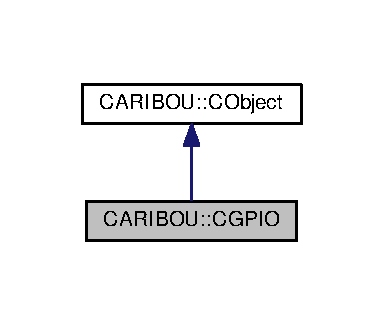
\includegraphics[width=184pt]{class_c_a_r_i_b_o_u_1_1_c_g_p_i_o__inherit__graph}
\end{center}
\end{figure}


Collaboration diagram for C\-A\-R\-I\-B\-O\-U\-:\-:C\-G\-P\-I\-O\-:\nopagebreak
\begin{figure}[H]
\begin{center}
\leavevmode
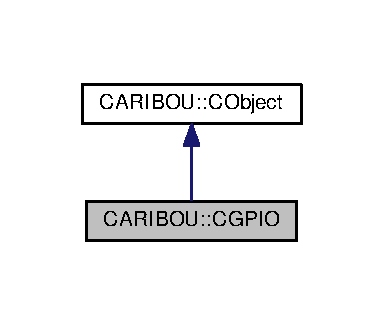
\includegraphics[width=184pt]{class_c_a_r_i_b_o_u_1_1_c_g_p_i_o__coll__graph}
\end{center}
\end{figure}
\subsection*{Public Member Functions}
\begin{DoxyCompactItemize}
\item 
{\bf C\-G\-P\-I\-O} (caribou\-\_\-gpio\-\_\-t $\ast${\bf gpio})
\item 
{\bf C\-G\-P\-I\-O} (const {\bf C\-G\-P\-I\-O} \&other)
\item 
virtual {\bf $\sim$\-C\-G\-P\-I\-O} ()
\item 
virtual void {\bf set} ()
\begin{DoxyCompactList}\small\item\em Set the pins in the pinmask. \end{DoxyCompactList}\item 
virtual void {\bf reset} ()
\begin{DoxyCompactList}\small\item\em Set the pins in the pinmask. \end{DoxyCompactList}\item 
virtual void {\bf toggle} ()
\begin{DoxyCompactList}\small\item\em Toggle the pin(s) in the pinmask. \end{DoxyCompactList}\item 
virtual void {\bf toggle} (uint32\-\_\-t msec)
\begin{DoxyCompactList}\small\item\em Toggle the pin at preset frequency. \end{DoxyCompactList}\item 
virtual void {\bf oneshot} (uint32\-\_\-t msec)
\begin{DoxyCompactList}\small\item\em Toggle the pin at preset frequency -\/ once. \end{DoxyCompactList}\item 
virtual chip\-\_\-gpio\-\_\-pinmask\-\_\-t {\bf state} ()
\begin{DoxyCompactList}\small\item\em Get the state of the pins according to the pinmask. \end{DoxyCompactList}\item 
virtual chip\-\_\-gpio\-\_\-pinmask\-\_\-t {\bf pinmask} ()
\begin{DoxyCompactList}\small\item\em Get the pin mask. \end{DoxyCompactList}\end{DoxyCompactItemize}
\subsection*{Protected Member Functions}
\begin{DoxyCompactItemize}
\item 
caribou\-\_\-gpio\-\_\-t $\ast$ {\bf gpio} ()
\item 
virtual void {\bf event} ({\bf C\-Event} $\ast$e)
\begin{DoxyCompactList}\small\item\em receive a queued event, the complement of \doxyref{C\-Object\-::dispatch(\-C\-Event$\ast$)}{p.}{class_c_a_r_i_b_o_u_1_1_c_object_a8aa02620cb58d4e2d3e19999aa0fbfe7}. \end{DoxyCompactList}\end{DoxyCompactItemize}
\subsection*{Protected Attributes}
\begin{DoxyCompactItemize}
\item 
caribou\-\_\-gpio\-\_\-t {\bf m\-G\-P\-I\-O}
\end{DoxyCompactItemize}
\subsection*{Additional Inherited Members}


\subsection{Detailed Description}


Definition at line 25 of file cgpio.\-h.



\subsection{Constructor \& Destructor Documentation}
\index{C\-A\-R\-I\-B\-O\-U\-::\-C\-G\-P\-I\-O@{C\-A\-R\-I\-B\-O\-U\-::\-C\-G\-P\-I\-O}!C\-G\-P\-I\-O@{C\-G\-P\-I\-O}}
\index{C\-G\-P\-I\-O@{C\-G\-P\-I\-O}!CARIBOU::CGPIO@{C\-A\-R\-I\-B\-O\-U\-::\-C\-G\-P\-I\-O}}
\subsubsection[{C\-G\-P\-I\-O}]{\setlength{\rightskip}{0pt plus 5cm}C\-A\-R\-I\-B\-O\-U\-::\-C\-G\-P\-I\-O\-::\-C\-G\-P\-I\-O (
\begin{DoxyParamCaption}
\item[{caribou\-\_\-gpio\-\_\-t $\ast$}]{gpio}
\end{DoxyParamCaption}
)}\label{class_c_a_r_i_b_o_u_1_1_c_g_p_i_o_a01b44f85b71b6a503a11ccbfcf528420}


Definition at line 24 of file cgpio.\-cpp.

\index{C\-A\-R\-I\-B\-O\-U\-::\-C\-G\-P\-I\-O@{C\-A\-R\-I\-B\-O\-U\-::\-C\-G\-P\-I\-O}!C\-G\-P\-I\-O@{C\-G\-P\-I\-O}}
\index{C\-G\-P\-I\-O@{C\-G\-P\-I\-O}!CARIBOU::CGPIO@{C\-A\-R\-I\-B\-O\-U\-::\-C\-G\-P\-I\-O}}
\subsubsection[{C\-G\-P\-I\-O}]{\setlength{\rightskip}{0pt plus 5cm}C\-A\-R\-I\-B\-O\-U\-::\-C\-G\-P\-I\-O\-::\-C\-G\-P\-I\-O (
\begin{DoxyParamCaption}
\item[{const {\bf C\-G\-P\-I\-O} \&}]{other}
\end{DoxyParamCaption}
)}\label{class_c_a_r_i_b_o_u_1_1_c_g_p_i_o_ad2703ba01f7124317243aaa8f636e104}


Definition at line 35 of file cgpio.\-cpp.

\index{C\-A\-R\-I\-B\-O\-U\-::\-C\-G\-P\-I\-O@{C\-A\-R\-I\-B\-O\-U\-::\-C\-G\-P\-I\-O}!$\sim$\-C\-G\-P\-I\-O@{$\sim$\-C\-G\-P\-I\-O}}
\index{$\sim$\-C\-G\-P\-I\-O@{$\sim$\-C\-G\-P\-I\-O}!CARIBOU::CGPIO@{C\-A\-R\-I\-B\-O\-U\-::\-C\-G\-P\-I\-O}}
\subsubsection[{$\sim$\-C\-G\-P\-I\-O}]{\setlength{\rightskip}{0pt plus 5cm}C\-A\-R\-I\-B\-O\-U\-::\-C\-G\-P\-I\-O\-::$\sim$\-C\-G\-P\-I\-O (
\begin{DoxyParamCaption}
{}
\end{DoxyParamCaption}
)\hspace{0.3cm}{\ttfamily [virtual]}}\label{class_c_a_r_i_b_o_u_1_1_c_g_p_i_o_ab41c45932deb734f32209512c37a683c}


Definition at line 42 of file cgpio.\-cpp.



\subsection{Member Function Documentation}
\index{C\-A\-R\-I\-B\-O\-U\-::\-C\-G\-P\-I\-O@{C\-A\-R\-I\-B\-O\-U\-::\-C\-G\-P\-I\-O}!event@{event}}
\index{event@{event}!CARIBOU::CGPIO@{C\-A\-R\-I\-B\-O\-U\-::\-C\-G\-P\-I\-O}}
\subsubsection[{event}]{\setlength{\rightskip}{0pt plus 5cm}void C\-A\-R\-I\-B\-O\-U\-::\-C\-G\-P\-I\-O\-::event (
\begin{DoxyParamCaption}
\item[{{\bf C\-Event} $\ast$}]{e}
\end{DoxyParamCaption}
)\hspace{0.3cm}{\ttfamily [protected]}, {\ttfamily [virtual]}}\label{class_c_a_r_i_b_o_u_1_1_c_g_p_i_o_ab67320903fc92646816756ab6507be12}


receive a queued event, the complement of \doxyref{C\-Object\-::dispatch(\-C\-Event$\ast$)}{p.}{class_c_a_r_i_b_o_u_1_1_c_object_a8aa02620cb58d4e2d3e19999aa0fbfe7}. 

Process Events. 

Reimplemented from {\bf C\-A\-R\-I\-B\-O\-U\-::\-C\-Object} \doxyref{}{p.}{class_c_a_r_i_b_o_u_1_1_c_object_a3e0d51872e9834666d064c716340bbdd}.



Definition at line 114 of file cgpio.\-cpp.

\index{C\-A\-R\-I\-B\-O\-U\-::\-C\-G\-P\-I\-O@{C\-A\-R\-I\-B\-O\-U\-::\-C\-G\-P\-I\-O}!gpio@{gpio}}
\index{gpio@{gpio}!CARIBOU::CGPIO@{C\-A\-R\-I\-B\-O\-U\-::\-C\-G\-P\-I\-O}}
\subsubsection[{gpio}]{\setlength{\rightskip}{0pt plus 5cm}caribou\-\_\-gpio\-\_\-t$\ast$ C\-A\-R\-I\-B\-O\-U\-::\-C\-G\-P\-I\-O\-::gpio (
\begin{DoxyParamCaption}
{}
\end{DoxyParamCaption}
)\hspace{0.3cm}{\ttfamily [inline]}, {\ttfamily [protected]}}\label{class_c_a_r_i_b_o_u_1_1_c_g_p_i_o_ae802b787b04f0a639adc51bbbca2b75e}


Definition at line 42 of file cgpio.\-h.

\index{C\-A\-R\-I\-B\-O\-U\-::\-C\-G\-P\-I\-O@{C\-A\-R\-I\-B\-O\-U\-::\-C\-G\-P\-I\-O}!oneshot@{oneshot}}
\index{oneshot@{oneshot}!CARIBOU::CGPIO@{C\-A\-R\-I\-B\-O\-U\-::\-C\-G\-P\-I\-O}}
\subsubsection[{oneshot}]{\setlength{\rightskip}{0pt plus 5cm}void C\-A\-R\-I\-B\-O\-U\-::\-C\-G\-P\-I\-O\-::oneshot (
\begin{DoxyParamCaption}
\item[{uint32\-\_\-t}]{msec}
\end{DoxyParamCaption}
)\hspace{0.3cm}{\ttfamily [virtual]}}\label{class_c_a_r_i_b_o_u_1_1_c_g_p_i_o_a955c8ab55bfd9cd70728ad495cf8bf14}


Toggle the pin at preset frequency -\/ once. 


\begin{DoxyParams}{Parameters}
{\em msec} & number of milliseconds per period. \\
\hline
\end{DoxyParams}


Definition at line 105 of file cgpio.\-cpp.

\index{C\-A\-R\-I\-B\-O\-U\-::\-C\-G\-P\-I\-O@{C\-A\-R\-I\-B\-O\-U\-::\-C\-G\-P\-I\-O}!pinmask@{pinmask}}
\index{pinmask@{pinmask}!CARIBOU::CGPIO@{C\-A\-R\-I\-B\-O\-U\-::\-C\-G\-P\-I\-O}}
\subsubsection[{pinmask}]{\setlength{\rightskip}{0pt plus 5cm}chip\-\_\-gpio\-\_\-pinmask\-\_\-t C\-A\-R\-I\-B\-O\-U\-::\-C\-G\-P\-I\-O\-::pinmask (
\begin{DoxyParamCaption}
{}
\end{DoxyParamCaption}
)\hspace{0.3cm}{\ttfamily [virtual]}}\label{class_c_a_r_i_b_o_u_1_1_c_g_p_i_o_af97edf120e08f968fa3081343994cb71}


Get the pin mask. 



Definition at line 58 of file cgpio.\-cpp.

\index{C\-A\-R\-I\-B\-O\-U\-::\-C\-G\-P\-I\-O@{C\-A\-R\-I\-B\-O\-U\-::\-C\-G\-P\-I\-O}!reset@{reset}}
\index{reset@{reset}!CARIBOU::CGPIO@{C\-A\-R\-I\-B\-O\-U\-::\-C\-G\-P\-I\-O}}
\subsubsection[{reset}]{\setlength{\rightskip}{0pt plus 5cm}void C\-A\-R\-I\-B\-O\-U\-::\-C\-G\-P\-I\-O\-::reset (
\begin{DoxyParamCaption}
{}
\end{DoxyParamCaption}
)\hspace{0.3cm}{\ttfamily [virtual]}}\label{class_c_a_r_i_b_o_u_1_1_c_g_p_i_o_a98c5508e3a8841d26d1b84e5e557cf2a}


Set the pins in the pinmask. 



Definition at line 75 of file cgpio.\-cpp.

\index{C\-A\-R\-I\-B\-O\-U\-::\-C\-G\-P\-I\-O@{C\-A\-R\-I\-B\-O\-U\-::\-C\-G\-P\-I\-O}!set@{set}}
\index{set@{set}!CARIBOU::CGPIO@{C\-A\-R\-I\-B\-O\-U\-::\-C\-G\-P\-I\-O}}
\subsubsection[{set}]{\setlength{\rightskip}{0pt plus 5cm}void C\-A\-R\-I\-B\-O\-U\-::\-C\-G\-P\-I\-O\-::set (
\begin{DoxyParamCaption}
{}
\end{DoxyParamCaption}
)\hspace{0.3cm}{\ttfamily [virtual]}}\label{class_c_a_r_i_b_o_u_1_1_c_g_p_i_o_af152e2876fff5bbe7d14fabfc17701b4}


Set the pins in the pinmask. 



Definition at line 67 of file cgpio.\-cpp.

\index{C\-A\-R\-I\-B\-O\-U\-::\-C\-G\-P\-I\-O@{C\-A\-R\-I\-B\-O\-U\-::\-C\-G\-P\-I\-O}!state@{state}}
\index{state@{state}!CARIBOU::CGPIO@{C\-A\-R\-I\-B\-O\-U\-::\-C\-G\-P\-I\-O}}
\subsubsection[{state}]{\setlength{\rightskip}{0pt plus 5cm}chip\-\_\-gpio\-\_\-pinmask\-\_\-t C\-A\-R\-I\-B\-O\-U\-::\-C\-G\-P\-I\-O\-::state (
\begin{DoxyParamCaption}
{}
\end{DoxyParamCaption}
)\hspace{0.3cm}{\ttfamily [virtual]}}\label{class_c_a_r_i_b_o_u_1_1_c_g_p_i_o_a69a24c088f1f210b5fc955a429b7ea8f}


Get the state of the pins according to the pinmask. 



Definition at line 49 of file cgpio.\-cpp.

\index{C\-A\-R\-I\-B\-O\-U\-::\-C\-G\-P\-I\-O@{C\-A\-R\-I\-B\-O\-U\-::\-C\-G\-P\-I\-O}!toggle@{toggle}}
\index{toggle@{toggle}!CARIBOU::CGPIO@{C\-A\-R\-I\-B\-O\-U\-::\-C\-G\-P\-I\-O}}
\subsubsection[{toggle}]{\setlength{\rightskip}{0pt plus 5cm}void C\-A\-R\-I\-B\-O\-U\-::\-C\-G\-P\-I\-O\-::toggle (
\begin{DoxyParamCaption}
{}
\end{DoxyParamCaption}
)\hspace{0.3cm}{\ttfamily [virtual]}}\label{class_c_a_r_i_b_o_u_1_1_c_g_p_i_o_a877f35df323325f826c81ec4291682db}


Toggle the pin(s) in the pinmask. 



Definition at line 83 of file cgpio.\-cpp.

\index{C\-A\-R\-I\-B\-O\-U\-::\-C\-G\-P\-I\-O@{C\-A\-R\-I\-B\-O\-U\-::\-C\-G\-P\-I\-O}!toggle@{toggle}}
\index{toggle@{toggle}!CARIBOU::CGPIO@{C\-A\-R\-I\-B\-O\-U\-::\-C\-G\-P\-I\-O}}
\subsubsection[{toggle}]{\setlength{\rightskip}{0pt plus 5cm}void C\-A\-R\-I\-B\-O\-U\-::\-C\-G\-P\-I\-O\-::toggle (
\begin{DoxyParamCaption}
\item[{uint32\-\_\-t}]{msec}
\end{DoxyParamCaption}
)\hspace{0.3cm}{\ttfamily [virtual]}}\label{class_c_a_r_i_b_o_u_1_1_c_g_p_i_o_ae988131fb9154213b1df1cc86e76cc11}


Toggle the pin at preset frequency. 


\begin{DoxyParams}{Parameters}
{\em msec} & number of milliseconds per period. \\
\hline
\end{DoxyParams}


Definition at line 92 of file cgpio.\-cpp.



\subsection{Member Data Documentation}
\index{C\-A\-R\-I\-B\-O\-U\-::\-C\-G\-P\-I\-O@{C\-A\-R\-I\-B\-O\-U\-::\-C\-G\-P\-I\-O}!m\-G\-P\-I\-O@{m\-G\-P\-I\-O}}
\index{m\-G\-P\-I\-O@{m\-G\-P\-I\-O}!CARIBOU::CGPIO@{C\-A\-R\-I\-B\-O\-U\-::\-C\-G\-P\-I\-O}}
\subsubsection[{m\-G\-P\-I\-O}]{\setlength{\rightskip}{0pt plus 5cm}caribou\-\_\-gpio\-\_\-t C\-A\-R\-I\-B\-O\-U\-::\-C\-G\-P\-I\-O\-::m\-G\-P\-I\-O\hspace{0.3cm}{\ttfamily [protected]}}\label{class_c_a_r_i_b_o_u_1_1_c_g_p_i_o_a909fd9b0768fe638329d76cf47172df3}


Definition at line 45 of file cgpio.\-h.



The documentation for this class was generated from the following files\-:\begin{DoxyCompactItemize}
\item 
include/caribou++/{\bf cgpio.\-h}\item 
src/{\bf cgpio.\-cpp}\end{DoxyCompactItemize}

\section{C\+A\+R\+I\+B\+OU\+:\+:C\+List$<$ T $>$ Class Template Reference}
\label{class_c_a_r_i_b_o_u_1_1_c_list}\index{C\+A\+R\+I\+B\+O\+U\+::\+C\+List$<$ T $>$@{C\+A\+R\+I\+B\+O\+U\+::\+C\+List$<$ T $>$}}


List template class.  




{\ttfamily \#include $<$cobject.\+h$>$}



Collaboration diagram for C\+A\+R\+I\+B\+OU\+:\+:C\+List$<$ T $>$\+:\nopagebreak
\begin{figure}[H]
\begin{center}
\leavevmode
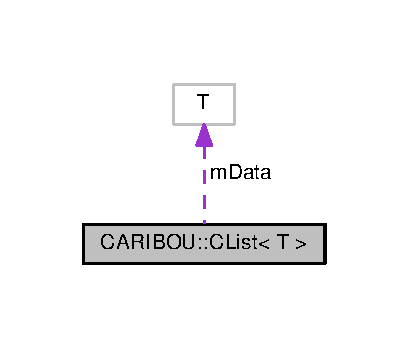
\includegraphics[width=196pt]{class_c_a_r_i_b_o_u_1_1_c_list__coll__graph}
\end{center}
\end{figure}
\subsection*{Public Member Functions}
\begin{DoxyCompactItemize}
\item 
{\bf C\+List} ()
\item 
{\bf C\+List} (const {\bf C\+List}$<$ T $>$ \&other)
\item 
{\bf $\sim$\+C\+List} ()
\item 
{\bf C\+List}$<$ T $>$ \& {\bf operator=} (const {\bf C\+List}$<$ T $>$ \&other)
\item 
void {\bf copy} (const {\bf C\+List}$<$ T $>$ \&other)
\item 
virtual void {\bf clear} ()
\item 
void {\bf dispose} ()
\begin{DoxyCompactList}\small\item\em dispose of objects which where allocated with new operator. \end{DoxyCompactList}\item 
uint32\+\_\+t {\bf resize} (uint32\+\_\+t {\bf size})
\item 
bool {\bf append} (T {\bf data})
\item 
bool {\bf insert} (T {\bf data}, int index=-\/1)
\item 
{\bf C\+List}$<$ T $>$ \& {\bf set} (uint32\+\_\+t index, T {\bf data})
\item 
const T {\bf at} (uint32\+\_\+t index)
\item 
const T {\bf take} (uint32\+\_\+t index)
\item 
const T {\bf take\+First} ()
\item 
const T {\bf take\+Last} ()
\item 
int32\+\_\+t {\bf index\+Of} (T {\bf data})
\item 
uint32\+\_\+t {\bf count} ()
\item 
uint32\+\_\+t {\bf size} ()
\item 
T $\ast$ {\bf data} ()
\item 
bool {\bf is\+Null} ()
\item 
bool {\bf is\+Empty} ()
\end{DoxyCompactItemize}
\subsection*{Protected Attributes}
\begin{DoxyCompactItemize}
\item 
uint32\+\_\+t {\bf m\+Size}
\item 
T $\ast$ {\bf m\+Data}
\end{DoxyCompactItemize}


\subsection{Detailed Description}
\subsubsection*{template$<$class T$>$\\*
class C\+A\+R\+I\+B\+O\+U\+::\+C\+List$<$ T $>$}

List template class. 

\begin{DoxyAuthor}{Author}
Mike Sharkey {\tt mike@pikeaero.\+com} 
\end{DoxyAuthor}


Definition at line 33 of file cobject.\+h.



\subsection{Constructor \& Destructor Documentation}
\index{C\+A\+R\+I\+B\+O\+U\+::\+C\+List@{C\+A\+R\+I\+B\+O\+U\+::\+C\+List}!C\+List@{C\+List}}
\index{C\+List@{C\+List}!C\+A\+R\+I\+B\+O\+U\+::\+C\+List@{C\+A\+R\+I\+B\+O\+U\+::\+C\+List}}
\subsubsection[{C\+List()}]{\setlength{\rightskip}{0pt plus 5cm}template$<$class T $>$ {\bf C\+A\+R\+I\+B\+O\+U\+::\+C\+List}$<$ T $>$\+::{\bf C\+List} (
\begin{DoxyParamCaption}
{}
\end{DoxyParamCaption}
)}\label{class_c_a_r_i_b_o_u_1_1_c_list_a4e17d65859ebc304d70643b83267195f}


Definition at line 78 of file clist.\+h.

\index{C\+A\+R\+I\+B\+O\+U\+::\+C\+List@{C\+A\+R\+I\+B\+O\+U\+::\+C\+List}!C\+List@{C\+List}}
\index{C\+List@{C\+List}!C\+A\+R\+I\+B\+O\+U\+::\+C\+List@{C\+A\+R\+I\+B\+O\+U\+::\+C\+List}}
\subsubsection[{C\+List(const C\+List$<$ T $>$ \&other)}]{\setlength{\rightskip}{0pt plus 5cm}template$<$class T$>$ {\bf C\+A\+R\+I\+B\+O\+U\+::\+C\+List}$<$ T $>$\+::{\bf C\+List} (
\begin{DoxyParamCaption}
\item[{const {\bf C\+List}$<$ T $>$ \&}]{other}
\end{DoxyParamCaption}
)}\label{class_c_a_r_i_b_o_u_1_1_c_list_acbbab9e82b60a00de366dff2201ecfbc}


Definition at line 84 of file clist.\+h.

\index{C\+A\+R\+I\+B\+O\+U\+::\+C\+List@{C\+A\+R\+I\+B\+O\+U\+::\+C\+List}!````~C\+List@{$\sim$\+C\+List}}
\index{````~C\+List@{$\sim$\+C\+List}!C\+A\+R\+I\+B\+O\+U\+::\+C\+List@{C\+A\+R\+I\+B\+O\+U\+::\+C\+List}}
\subsubsection[{$\sim$\+C\+List()}]{\setlength{\rightskip}{0pt plus 5cm}template$<$class T $>$ {\bf C\+A\+R\+I\+B\+O\+U\+::\+C\+List}$<$ T $>$\+::$\sim${\bf C\+List} (
\begin{DoxyParamCaption}
{}
\end{DoxyParamCaption}
)}\label{class_c_a_r_i_b_o_u_1_1_c_list_a820a648b5cbc989e382caf85f4ccbc98}


Definition at line 107 of file clist.\+h.



\subsection{Member Function Documentation}
\index{C\+A\+R\+I\+B\+O\+U\+::\+C\+List@{C\+A\+R\+I\+B\+O\+U\+::\+C\+List}!append@{append}}
\index{append@{append}!C\+A\+R\+I\+B\+O\+U\+::\+C\+List@{C\+A\+R\+I\+B\+O\+U\+::\+C\+List}}
\subsubsection[{append(\+T data)}]{\setlength{\rightskip}{0pt plus 5cm}template$<$class T$>$ bool {\bf C\+A\+R\+I\+B\+O\+U\+::\+C\+List}$<$ T $>$\+::append (
\begin{DoxyParamCaption}
\item[{T}]{data}
\end{DoxyParamCaption}
)}\label{class_c_a_r_i_b_o_u_1_1_c_list_ac017abd07459d047bac7d0d200eb7cac}


Definition at line 168 of file clist.\+h.

\index{C\+A\+R\+I\+B\+O\+U\+::\+C\+List@{C\+A\+R\+I\+B\+O\+U\+::\+C\+List}!at@{at}}
\index{at@{at}!C\+A\+R\+I\+B\+O\+U\+::\+C\+List@{C\+A\+R\+I\+B\+O\+U\+::\+C\+List}}
\subsubsection[{at(uint32\+\_\+t index)}]{\setlength{\rightskip}{0pt plus 5cm}template$<$class T $>$ const T {\bf C\+A\+R\+I\+B\+O\+U\+::\+C\+List}$<$ T $>$\+::at (
\begin{DoxyParamCaption}
\item[{uint32\+\_\+t}]{index}
\end{DoxyParamCaption}
)}\label{class_c_a_r_i_b_o_u_1_1_c_list_a9d1e4b9f2ea2e9abcc616df41e9f6a25}


Definition at line 209 of file clist.\+h.

\index{C\+A\+R\+I\+B\+O\+U\+::\+C\+List@{C\+A\+R\+I\+B\+O\+U\+::\+C\+List}!clear@{clear}}
\index{clear@{clear}!C\+A\+R\+I\+B\+O\+U\+::\+C\+List@{C\+A\+R\+I\+B\+O\+U\+::\+C\+List}}
\subsubsection[{clear()}]{\setlength{\rightskip}{0pt plus 5cm}template$<$class T $>$ void {\bf C\+A\+R\+I\+B\+O\+U\+::\+C\+List}$<$ T $>$\+::clear (
\begin{DoxyParamCaption}
{}
\end{DoxyParamCaption}
)\hspace{0.3cm}{\ttfamily [virtual]}}\label{class_c_a_r_i_b_o_u_1_1_c_list_a63ccc0ca8665929eb1c0330c45b305e0}


Definition at line 120 of file clist.\+h.

\index{C\+A\+R\+I\+B\+O\+U\+::\+C\+List@{C\+A\+R\+I\+B\+O\+U\+::\+C\+List}!copy@{copy}}
\index{copy@{copy}!C\+A\+R\+I\+B\+O\+U\+::\+C\+List@{C\+A\+R\+I\+B\+O\+U\+::\+C\+List}}
\subsubsection[{copy(const C\+List$<$ T $>$ \&other)}]{\setlength{\rightskip}{0pt plus 5cm}template$<$class T$>$ void {\bf C\+A\+R\+I\+B\+O\+U\+::\+C\+List}$<$ T $>$\+::copy (
\begin{DoxyParamCaption}
\item[{const {\bf C\+List}$<$ T $>$ \&}]{other}
\end{DoxyParamCaption}
)}\label{class_c_a_r_i_b_o_u_1_1_c_list_acdee41eaeb90c7c516dd1abba877c113}


Definition at line 112 of file clist.\+h.

\index{C\+A\+R\+I\+B\+O\+U\+::\+C\+List@{C\+A\+R\+I\+B\+O\+U\+::\+C\+List}!count@{count}}
\index{count@{count}!C\+A\+R\+I\+B\+O\+U\+::\+C\+List@{C\+A\+R\+I\+B\+O\+U\+::\+C\+List}}
\subsubsection[{count()}]{\setlength{\rightskip}{0pt plus 5cm}template$<$class T$>$ uint32\+\_\+t {\bf C\+A\+R\+I\+B\+O\+U\+::\+C\+List}$<$ T $>$\+::count (
\begin{DoxyParamCaption}
{}
\end{DoxyParamCaption}
)\hspace{0.3cm}{\ttfamily [inline]}}\label{class_c_a_r_i_b_o_u_1_1_c_list_a9fe7203a1930a83ad34e4853ef8fedbd}


Definition at line 57 of file clist.\+h.

\index{C\+A\+R\+I\+B\+O\+U\+::\+C\+List@{C\+A\+R\+I\+B\+O\+U\+::\+C\+List}!data@{data}}
\index{data@{data}!C\+A\+R\+I\+B\+O\+U\+::\+C\+List@{C\+A\+R\+I\+B\+O\+U\+::\+C\+List}}
\subsubsection[{data()}]{\setlength{\rightskip}{0pt plus 5cm}template$<$class T $>$ T $\ast$ {\bf C\+A\+R\+I\+B\+O\+U\+::\+C\+List}$<$ T $>$\+::data (
\begin{DoxyParamCaption}
{}
\end{DoxyParamCaption}
)}\label{class_c_a_r_i_b_o_u_1_1_c_list_a4a8f74c488da22f4ef2dd4068709a042}


Definition at line 268 of file clist.\+h.

\index{C\+A\+R\+I\+B\+O\+U\+::\+C\+List@{C\+A\+R\+I\+B\+O\+U\+::\+C\+List}!dispose@{dispose}}
\index{dispose@{dispose}!C\+A\+R\+I\+B\+O\+U\+::\+C\+List@{C\+A\+R\+I\+B\+O\+U\+::\+C\+List}}
\subsubsection[{dispose()}]{\setlength{\rightskip}{0pt plus 5cm}template$<$class T $>$ void {\bf C\+A\+R\+I\+B\+O\+U\+::\+C\+List}$<$ T $>$\+::dispose (
\begin{DoxyParamCaption}
{}
\end{DoxyParamCaption}
)}\label{class_c_a_r_i_b_o_u_1_1_c_list_ab5a899258041d8fae1863ccdbd4b7803}


dispose of objects which where allocated with new operator. 



Definition at line 133 of file clist.\+h.

\index{C\+A\+R\+I\+B\+O\+U\+::\+C\+List@{C\+A\+R\+I\+B\+O\+U\+::\+C\+List}!index\+Of@{index\+Of}}
\index{index\+Of@{index\+Of}!C\+A\+R\+I\+B\+O\+U\+::\+C\+List@{C\+A\+R\+I\+B\+O\+U\+::\+C\+List}}
\subsubsection[{index\+Of(\+T data)}]{\setlength{\rightskip}{0pt plus 5cm}template$<$class T$>$ int32\+\_\+t {\bf C\+A\+R\+I\+B\+O\+U\+::\+C\+List}$<$ T $>$\+::index\+Of (
\begin{DoxyParamCaption}
\item[{T}]{data}
\end{DoxyParamCaption}
)}\label{class_c_a_r_i_b_o_u_1_1_c_list_acfcf1eb9fdb4ea11ffb37dd2f489ec27}


Definition at line 256 of file clist.\+h.

\index{C\+A\+R\+I\+B\+O\+U\+::\+C\+List@{C\+A\+R\+I\+B\+O\+U\+::\+C\+List}!insert@{insert}}
\index{insert@{insert}!C\+A\+R\+I\+B\+O\+U\+::\+C\+List@{C\+A\+R\+I\+B\+O\+U\+::\+C\+List}}
\subsubsection[{insert(\+T data, int index=-\/1)}]{\setlength{\rightskip}{0pt plus 5cm}template$<$class T$>$ bool {\bf C\+A\+R\+I\+B\+O\+U\+::\+C\+List}$<$ T $>$\+::insert (
\begin{DoxyParamCaption}
\item[{T}]{data, }
\item[{int}]{index = {\ttfamily -\/1}}
\end{DoxyParamCaption}
)}\label{class_c_a_r_i_b_o_u_1_1_c_list_ae6f91d52e6c42c9e536fe952d50b6363}


Definition at line 179 of file clist.\+h.

\index{C\+A\+R\+I\+B\+O\+U\+::\+C\+List@{C\+A\+R\+I\+B\+O\+U\+::\+C\+List}!is\+Empty@{is\+Empty}}
\index{is\+Empty@{is\+Empty}!C\+A\+R\+I\+B\+O\+U\+::\+C\+List@{C\+A\+R\+I\+B\+O\+U\+::\+C\+List}}
\subsubsection[{is\+Empty()}]{\setlength{\rightskip}{0pt plus 5cm}template$<$class T $>$ bool {\bf C\+A\+R\+I\+B\+O\+U\+::\+C\+List}$<$ T $>$\+::is\+Empty (
\begin{DoxyParamCaption}
{}
\end{DoxyParamCaption}
)}\label{class_c_a_r_i_b_o_u_1_1_c_list_a0491db3e887fb9a1dd2cff456814a1b4}


Definition at line 278 of file clist.\+h.

\index{C\+A\+R\+I\+B\+O\+U\+::\+C\+List@{C\+A\+R\+I\+B\+O\+U\+::\+C\+List}!is\+Null@{is\+Null}}
\index{is\+Null@{is\+Null}!C\+A\+R\+I\+B\+O\+U\+::\+C\+List@{C\+A\+R\+I\+B\+O\+U\+::\+C\+List}}
\subsubsection[{is\+Null()}]{\setlength{\rightskip}{0pt plus 5cm}template$<$class T $>$ bool {\bf C\+A\+R\+I\+B\+O\+U\+::\+C\+List}$<$ T $>$\+::is\+Null (
\begin{DoxyParamCaption}
{}
\end{DoxyParamCaption}
)}\label{class_c_a_r_i_b_o_u_1_1_c_list_a588b5737a2affcaca2ee000db090f2db}


Definition at line 273 of file clist.\+h.

\index{C\+A\+R\+I\+B\+O\+U\+::\+C\+List@{C\+A\+R\+I\+B\+O\+U\+::\+C\+List}!operator=@{operator=}}
\index{operator=@{operator=}!C\+A\+R\+I\+B\+O\+U\+::\+C\+List@{C\+A\+R\+I\+B\+O\+U\+::\+C\+List}}
\subsubsection[{operator=(const C\+List$<$ T $>$ \&other)}]{\setlength{\rightskip}{0pt plus 5cm}template$<$class T$>$ {\bf C\+List}$<$T$>$\& {\bf C\+A\+R\+I\+B\+O\+U\+::\+C\+List}$<$ T $>$\+::operator= (
\begin{DoxyParamCaption}
\item[{const {\bf C\+List}$<$ T $>$ \&}]{other}
\end{DoxyParamCaption}
)\hspace{0.3cm}{\ttfamily [inline]}}\label{class_c_a_r_i_b_o_u_1_1_c_list_a4839bb950dcf8e0c5fd3dbac8619ae75}


Definition at line 35 of file clist.\+h.

\index{C\+A\+R\+I\+B\+O\+U\+::\+C\+List@{C\+A\+R\+I\+B\+O\+U\+::\+C\+List}!resize@{resize}}
\index{resize@{resize}!C\+A\+R\+I\+B\+O\+U\+::\+C\+List@{C\+A\+R\+I\+B\+O\+U\+::\+C\+List}}
\subsubsection[{resize(uint32\+\_\+t size)}]{\setlength{\rightskip}{0pt plus 5cm}template$<$class T $>$ uint32\+\_\+t {\bf C\+A\+R\+I\+B\+O\+U\+::\+C\+List}$<$ T $>$\+::resize (
\begin{DoxyParamCaption}
\item[{uint32\+\_\+t}]{size}
\end{DoxyParamCaption}
)}\label{class_c_a_r_i_b_o_u_1_1_c_list_a1166ddd7beab7853c9e5a611de1b56bc}


Definition at line 143 of file clist.\+h.

\index{C\+A\+R\+I\+B\+O\+U\+::\+C\+List@{C\+A\+R\+I\+B\+O\+U\+::\+C\+List}!set@{set}}
\index{set@{set}!C\+A\+R\+I\+B\+O\+U\+::\+C\+List@{C\+A\+R\+I\+B\+O\+U\+::\+C\+List}}
\subsubsection[{set(uint32\+\_\+t index, T data)}]{\setlength{\rightskip}{0pt plus 5cm}template$<$class T$>$ {\bf C\+List}$<$ T $>$ \& {\bf C\+A\+R\+I\+B\+O\+U\+::\+C\+List}$<$ T $>$\+::set (
\begin{DoxyParamCaption}
\item[{uint32\+\_\+t}]{index, }
\item[{T}]{data}
\end{DoxyParamCaption}
)}\label{class_c_a_r_i_b_o_u_1_1_c_list_ad48332621b31c02fe8634f16bea5d1d2}


Definition at line 200 of file clist.\+h.

\index{C\+A\+R\+I\+B\+O\+U\+::\+C\+List@{C\+A\+R\+I\+B\+O\+U\+::\+C\+List}!size@{size}}
\index{size@{size}!C\+A\+R\+I\+B\+O\+U\+::\+C\+List@{C\+A\+R\+I\+B\+O\+U\+::\+C\+List}}
\subsubsection[{size()}]{\setlength{\rightskip}{0pt plus 5cm}template$<$class T$>$ uint32\+\_\+t {\bf C\+A\+R\+I\+B\+O\+U\+::\+C\+List}$<$ T $>$\+::size (
\begin{DoxyParamCaption}
{}
\end{DoxyParamCaption}
)\hspace{0.3cm}{\ttfamily [inline]}}\label{class_c_a_r_i_b_o_u_1_1_c_list_a6f376b4d8c138fc3fddfba09613d336f}


Definition at line 58 of file clist.\+h.

\index{C\+A\+R\+I\+B\+O\+U\+::\+C\+List@{C\+A\+R\+I\+B\+O\+U\+::\+C\+List}!take@{take}}
\index{take@{take}!C\+A\+R\+I\+B\+O\+U\+::\+C\+List@{C\+A\+R\+I\+B\+O\+U\+::\+C\+List}}
\subsubsection[{take(uint32\+\_\+t index)}]{\setlength{\rightskip}{0pt plus 5cm}template$<$class T $>$ const T {\bf C\+A\+R\+I\+B\+O\+U\+::\+C\+List}$<$ T $>$\+::take (
\begin{DoxyParamCaption}
\item[{uint32\+\_\+t}]{index}
\end{DoxyParamCaption}
)}\label{class_c_a_r_i_b_o_u_1_1_c_list_aa1914d592985a0c79f39e3eeba8abec6}


Definition at line 218 of file clist.\+h.

\index{C\+A\+R\+I\+B\+O\+U\+::\+C\+List@{C\+A\+R\+I\+B\+O\+U\+::\+C\+List}!take\+First@{take\+First}}
\index{take\+First@{take\+First}!C\+A\+R\+I\+B\+O\+U\+::\+C\+List@{C\+A\+R\+I\+B\+O\+U\+::\+C\+List}}
\subsubsection[{take\+First()}]{\setlength{\rightskip}{0pt plus 5cm}template$<$class T $>$ const T {\bf C\+A\+R\+I\+B\+O\+U\+::\+C\+List}$<$ T $>$\+::take\+First (
\begin{DoxyParamCaption}
{}
\end{DoxyParamCaption}
)}\label{class_c_a_r_i_b_o_u_1_1_c_list_a49e0f7bacda6ec6e6441f0029dee7c66}


Definition at line 248 of file clist.\+h.

\index{C\+A\+R\+I\+B\+O\+U\+::\+C\+List@{C\+A\+R\+I\+B\+O\+U\+::\+C\+List}!take\+Last@{take\+Last}}
\index{take\+Last@{take\+Last}!C\+A\+R\+I\+B\+O\+U\+::\+C\+List@{C\+A\+R\+I\+B\+O\+U\+::\+C\+List}}
\subsubsection[{take\+Last()}]{\setlength{\rightskip}{0pt plus 5cm}template$<$class T $>$ const T {\bf C\+A\+R\+I\+B\+O\+U\+::\+C\+List}$<$ T $>$\+::take\+Last (
\begin{DoxyParamCaption}
{}
\end{DoxyParamCaption}
)}\label{class_c_a_r_i_b_o_u_1_1_c_list_abbfc078eb4a1c365c67f1017b812fc3b}


Definition at line 236 of file clist.\+h.



\subsection{Member Data Documentation}
\index{C\+A\+R\+I\+B\+O\+U\+::\+C\+List@{C\+A\+R\+I\+B\+O\+U\+::\+C\+List}!m\+Data@{m\+Data}}
\index{m\+Data@{m\+Data}!C\+A\+R\+I\+B\+O\+U\+::\+C\+List@{C\+A\+R\+I\+B\+O\+U\+::\+C\+List}}
\subsubsection[{m\+Data}]{\setlength{\rightskip}{0pt plus 5cm}template$<$class T$>$ T$\ast$ {\bf C\+A\+R\+I\+B\+O\+U\+::\+C\+List}$<$ T $>$\+::m\+Data\hspace{0.3cm}{\ttfamily [protected]}}\label{class_c_a_r_i_b_o_u_1_1_c_list_a1ac3a8f0a74b498bec10132ea61189ae}


Definition at line 66 of file clist.\+h.

\index{C\+A\+R\+I\+B\+O\+U\+::\+C\+List@{C\+A\+R\+I\+B\+O\+U\+::\+C\+List}!m\+Size@{m\+Size}}
\index{m\+Size@{m\+Size}!C\+A\+R\+I\+B\+O\+U\+::\+C\+List@{C\+A\+R\+I\+B\+O\+U\+::\+C\+List}}
\subsubsection[{m\+Size}]{\setlength{\rightskip}{0pt plus 5cm}template$<$class T$>$ uint32\+\_\+t {\bf C\+A\+R\+I\+B\+O\+U\+::\+C\+List}$<$ T $>$\+::m\+Size\hspace{0.3cm}{\ttfamily [protected]}}\label{class_c_a_r_i_b_o_u_1_1_c_list_acc7f59d17696171e87e8aea3d2c65fd1}


Definition at line 65 of file clist.\+h.



The documentation for this class was generated from the following files\+:\begin{DoxyCompactItemize}
\item 
include/caribou++/{\bf cobject.\+h}\item 
include/caribou++/{\bf clist.\+h}\end{DoxyCompactItemize}

\section{C\-A\-R\-I\-B\-O\-U\-:\-:C\-Map$<$ K, T $>$ Class Template Reference}
\label{class_c_a_r_i_b_o_u_1_1_c_map}\index{C\-A\-R\-I\-B\-O\-U\-::\-C\-Map$<$ K, T $>$@{C\-A\-R\-I\-B\-O\-U\-::\-C\-Map$<$ K, T $>$}}


Keys must implement the =, ==, $>$, $<$ operators.  




{\ttfamily \#include $<$cmap.\-h$>$}



Collaboration diagram for C\-A\-R\-I\-B\-O\-U\-:\-:C\-Map$<$ K, T $>$\-:\nopagebreak
\begin{figure}[H]
\begin{center}
\leavevmode
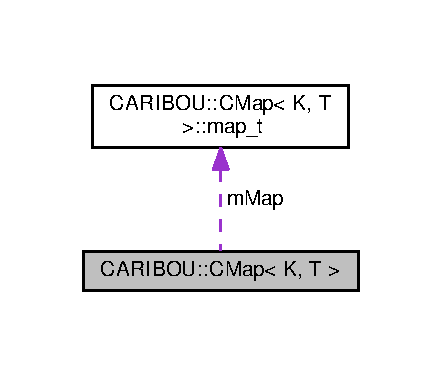
\includegraphics[width=212pt]{class_c_a_r_i_b_o_u_1_1_c_map__coll__graph}
\end{center}
\end{figure}
\subsection*{Classes}
\begin{DoxyCompactItemize}
\item 
struct {\bf map\-\_\-t}
\end{DoxyCompactItemize}
\subsection*{Public Member Functions}
\begin{DoxyCompactItemize}
\item 
{\bf C\-Map} ()
\item 
{\bf C\-Map} (const {\bf C\-Map}$<$ K, T $>$ \&other)
\item 
{\bf $\sim$\-C\-Map} ()
\item 
void {\bf clear} ()
\begin{DoxyCompactList}\small\item\em free storage \end{DoxyCompactList}\item 
void {\bf clear} (K key)
\begin{DoxyCompactList}\small\item\em free storage \end{DoxyCompactList}\item 
void {\bf dispose} ()
\begin{DoxyCompactList}\small\item\em Call the destructors on the elements -\/ does not free the storage. \end{DoxyCompactList}\item 
void {\bf dispose} (K key)
\begin{DoxyCompactList}\small\item\em Call the destructors on the elements -\/ does not free the storage. \end{DoxyCompactList}\item 
bool {\bf append} (K key, T {\bf data})
\item 
int32\-\_\-t {\bf index\-Of} (K key)
\begin{DoxyCompactList}\small\item\em Performa key search and retrieve the index of a map record based on the given key. \end{DoxyCompactList}\item 
const K {\bf at} (uint32\-\_\-t index)
\begin{DoxyCompactList}\small\item\em Retrieve the key at the given index. \end{DoxyCompactList}\item 
const T {\bf data\-At} (uint32\-\_\-t index)
\begin{DoxyCompactList}\small\item\em Perform a data lookup with a given key. \end{DoxyCompactList}\item 
const T {\bf data} (K key)
\begin{DoxyCompactList}\small\item\em Perform a data lookup with a given key. \end{DoxyCompactList}\item 
bool {\bf insert} (K key, T {\bf data}, int index)
\item 
{\bf C\-Map}$<$ K, T $>$ \& {\bf set} (K key, T {\bf data})
\item 
const T {\bf take} (uint32\-\_\-t index)
\item 
uint32\-\_\-t {\bf count} ()
\item 
uint32\-\_\-t {\bf size} ()
\item 
bool {\bf is\-Null} ()
\item 
bool {\bf is\-Empty} ()
\item 
{\bf C\-Map}$<$ K, T $>$ \& {\bf operator=} (const {\bf C\-Map}$<$ K, T $>$ \&other)
\end{DoxyCompactItemize}
\subsection*{Protected Member Functions}
\begin{DoxyCompactItemize}
\item 
uint32\-\_\-t {\bf resize} (uint32\-\_\-t {\bf size})
\end{DoxyCompactItemize}
\subsection*{Protected Attributes}
\begin{DoxyCompactItemize}
\item 
uint32\-\_\-t {\bf m\-Size}
\item 
{\bf map\-\_\-t} $\ast$$\ast$ {\bf m\-Map}
\end{DoxyCompactItemize}


\subsection{Detailed Description}
\subsubsection*{template$<$class K, class T$>$class C\-A\-R\-I\-B\-O\-U\-::\-C\-Map$<$ K, T $>$}

Keys must implement the =, ==, $>$, $<$ operators. 

Definition at line 27 of file cmap.\-h.



\subsection{Constructor \& Destructor Documentation}
\index{C\-A\-R\-I\-B\-O\-U\-::\-C\-Map@{C\-A\-R\-I\-B\-O\-U\-::\-C\-Map}!C\-Map@{C\-Map}}
\index{C\-Map@{C\-Map}!CARIBOU::CMap@{C\-A\-R\-I\-B\-O\-U\-::\-C\-Map}}
\subsubsection[{C\-Map}]{\setlength{\rightskip}{0pt plus 5cm}template$<$class K , class T $>$ {\bf C\-A\-R\-I\-B\-O\-U\-::\-C\-Map}$<$ K, T $>$\-::{\bf C\-Map} (
\begin{DoxyParamCaption}
{}
\end{DoxyParamCaption}
)}\label{class_c_a_r_i_b_o_u_1_1_c_map_a7251ce690588841ec5564d6fc9e67428}


Definition at line 144 of file cmap.\-h.

\index{C\-A\-R\-I\-B\-O\-U\-::\-C\-Map@{C\-A\-R\-I\-B\-O\-U\-::\-C\-Map}!C\-Map@{C\-Map}}
\index{C\-Map@{C\-Map}!CARIBOU::CMap@{C\-A\-R\-I\-B\-O\-U\-::\-C\-Map}}
\subsubsection[{C\-Map}]{\setlength{\rightskip}{0pt plus 5cm}template$<$class K, class T$>$ {\bf C\-A\-R\-I\-B\-O\-U\-::\-C\-Map}$<$ K, T $>$\-::{\bf C\-Map} (
\begin{DoxyParamCaption}
\item[{const {\bf C\-Map}$<$ K, T $>$ \&}]{other}
\end{DoxyParamCaption}
)}\label{class_c_a_r_i_b_o_u_1_1_c_map_a112a26a90e14587ba9fa86783447ffa1}


Definition at line 150 of file cmap.\-h.

\index{C\-A\-R\-I\-B\-O\-U\-::\-C\-Map@{C\-A\-R\-I\-B\-O\-U\-::\-C\-Map}!$\sim$\-C\-Map@{$\sim$\-C\-Map}}
\index{$\sim$\-C\-Map@{$\sim$\-C\-Map}!CARIBOU::CMap@{C\-A\-R\-I\-B\-O\-U\-::\-C\-Map}}
\subsubsection[{$\sim$\-C\-Map}]{\setlength{\rightskip}{0pt plus 5cm}template$<$class K , class T $>$ {\bf C\-A\-R\-I\-B\-O\-U\-::\-C\-Map}$<$ K, T $>$\-::$\sim${\bf C\-Map} (
\begin{DoxyParamCaption}
{}
\end{DoxyParamCaption}
)}\label{class_c_a_r_i_b_o_u_1_1_c_map_a659d387a1262e3c5bd0b12b478711af2}


Definition at line 163 of file cmap.\-h.



\subsection{Member Function Documentation}
\index{C\-A\-R\-I\-B\-O\-U\-::\-C\-Map@{C\-A\-R\-I\-B\-O\-U\-::\-C\-Map}!append@{append}}
\index{append@{append}!CARIBOU::CMap@{C\-A\-R\-I\-B\-O\-U\-::\-C\-Map}}
\subsubsection[{append}]{\setlength{\rightskip}{0pt plus 5cm}template$<$class K, class T$>$ bool {\bf C\-A\-R\-I\-B\-O\-U\-::\-C\-Map}$<$ K, T $>$\-::append (
\begin{DoxyParamCaption}
\item[{K}]{key, }
\item[{T}]{data}
\end{DoxyParamCaption}
)}\label{class_c_a_r_i_b_o_u_1_1_c_map_ac9dc557ba4b3fd602ea92f46b8344787}


Definition at line 235 of file cmap.\-h.

\index{C\-A\-R\-I\-B\-O\-U\-::\-C\-Map@{C\-A\-R\-I\-B\-O\-U\-::\-C\-Map}!at@{at}}
\index{at@{at}!CARIBOU::CMap@{C\-A\-R\-I\-B\-O\-U\-::\-C\-Map}}
\subsubsection[{at}]{\setlength{\rightskip}{0pt plus 5cm}template$<$class K , class T $>$ const K {\bf C\-A\-R\-I\-B\-O\-U\-::\-C\-Map}$<$ K, T $>$\-::at (
\begin{DoxyParamCaption}
\item[{uint32\-\_\-t}]{index}
\end{DoxyParamCaption}
)}\label{class_c_a_r_i_b_o_u_1_1_c_map_a51dd6526e740ab8ae093361733254044}


Retrieve the key at the given index. 



Definition at line 320 of file cmap.\-h.

\index{C\-A\-R\-I\-B\-O\-U\-::\-C\-Map@{C\-A\-R\-I\-B\-O\-U\-::\-C\-Map}!clear@{clear}}
\index{clear@{clear}!CARIBOU::CMap@{C\-A\-R\-I\-B\-O\-U\-::\-C\-Map}}
\subsubsection[{clear}]{\setlength{\rightskip}{0pt plus 5cm}template$<$class K , class T $>$ void {\bf C\-A\-R\-I\-B\-O\-U\-::\-C\-Map}$<$ K, T $>$\-::clear (
\begin{DoxyParamCaption}
{}
\end{DoxyParamCaption}
)}\label{class_c_a_r_i_b_o_u_1_1_c_map_a823a207005fff99da13571dbae0bc1dc}


free storage 



Definition at line 184 of file cmap.\-h.

\index{C\-A\-R\-I\-B\-O\-U\-::\-C\-Map@{C\-A\-R\-I\-B\-O\-U\-::\-C\-Map}!clear@{clear}}
\index{clear@{clear}!CARIBOU::CMap@{C\-A\-R\-I\-B\-O\-U\-::\-C\-Map}}
\subsubsection[{clear}]{\setlength{\rightskip}{0pt plus 5cm}template$<$class K, class T $>$ void {\bf C\-A\-R\-I\-B\-O\-U\-::\-C\-Map}$<$ K, T $>$\-::clear (
\begin{DoxyParamCaption}
\item[{K}]{key}
\end{DoxyParamCaption}
)}\label{class_c_a_r_i_b_o_u_1_1_c_map_a63409f5e0377e9d6c0f92cfaa920b2ef}


free storage 



Definition at line 201 of file cmap.\-h.

\index{C\-A\-R\-I\-B\-O\-U\-::\-C\-Map@{C\-A\-R\-I\-B\-O\-U\-::\-C\-Map}!count@{count}}
\index{count@{count}!CARIBOU::CMap@{C\-A\-R\-I\-B\-O\-U\-::\-C\-Map}}
\subsubsection[{count}]{\setlength{\rightskip}{0pt plus 5cm}template$<$class K, class T$>$ uint32\-\_\-t {\bf C\-A\-R\-I\-B\-O\-U\-::\-C\-Map}$<$ K, T $>$\-::count (
\begin{DoxyParamCaption}
{}
\end{DoxyParamCaption}
)\hspace{0.3cm}{\ttfamily [inline]}}\label{class_c_a_r_i_b_o_u_1_1_c_map_a57e2e469f07066498bbb170136951d6f}


Definition at line 46 of file cmap.\-h.

\index{C\-A\-R\-I\-B\-O\-U\-::\-C\-Map@{C\-A\-R\-I\-B\-O\-U\-::\-C\-Map}!data@{data}}
\index{data@{data}!CARIBOU::CMap@{C\-A\-R\-I\-B\-O\-U\-::\-C\-Map}}
\subsubsection[{data}]{\setlength{\rightskip}{0pt plus 5cm}template$<$class K, class T $>$ const T {\bf C\-A\-R\-I\-B\-O\-U\-::\-C\-Map}$<$ K, T $>$\-::data (
\begin{DoxyParamCaption}
\item[{K}]{key}
\end{DoxyParamCaption}
)}\label{class_c_a_r_i_b_o_u_1_1_c_map_a24a563b9416d61834dc57eb7ca135131}


Perform a data lookup with a given key. 


\begin{DoxyParams}{Parameters}
{\em key} & The key to search for. \\
\hline
\end{DoxyParams}
\begin{DoxyReturn}{Returns}
A copy of the data. 
\end{DoxyReturn}


Definition at line 293 of file cmap.\-h.

\index{C\-A\-R\-I\-B\-O\-U\-::\-C\-Map@{C\-A\-R\-I\-B\-O\-U\-::\-C\-Map}!data\-At@{data\-At}}
\index{data\-At@{data\-At}!CARIBOU::CMap@{C\-A\-R\-I\-B\-O\-U\-::\-C\-Map}}
\subsubsection[{data\-At}]{\setlength{\rightskip}{0pt plus 5cm}template$<$class K , class T $>$ const T {\bf C\-A\-R\-I\-B\-O\-U\-::\-C\-Map}$<$ K, T $>$\-::data\-At (
\begin{DoxyParamCaption}
\item[{uint32\-\_\-t}]{index}
\end{DoxyParamCaption}
)}\label{class_c_a_r_i_b_o_u_1_1_c_map_a678205d0eaa849e12a0460c9e7b67efb}


Perform a data lookup with a given key. 


\begin{DoxyParams}{Parameters}
{\em key} & The key to search for. \\
\hline
\end{DoxyParams}
\begin{DoxyReturn}{Returns}
A copy of the data. 
\end{DoxyReturn}


Definition at line 308 of file cmap.\-h.

\index{C\-A\-R\-I\-B\-O\-U\-::\-C\-Map@{C\-A\-R\-I\-B\-O\-U\-::\-C\-Map}!dispose@{dispose}}
\index{dispose@{dispose}!CARIBOU::CMap@{C\-A\-R\-I\-B\-O\-U\-::\-C\-Map}}
\subsubsection[{dispose}]{\setlength{\rightskip}{0pt plus 5cm}template$<$class K , class T $>$ void {\bf C\-A\-R\-I\-B\-O\-U\-::\-C\-Map}$<$ K, T $>$\-::dispose (
\begin{DoxyParamCaption}
{}
\end{DoxyParamCaption}
)}\label{class_c_a_r_i_b_o_u_1_1_c_map_a75644d199c3abd520a95922af4efb313}


Call the destructors on the elements -\/ does not free the storage. 



Definition at line 213 of file cmap.\-h.

\index{C\-A\-R\-I\-B\-O\-U\-::\-C\-Map@{C\-A\-R\-I\-B\-O\-U\-::\-C\-Map}!dispose@{dispose}}
\index{dispose@{dispose}!CARIBOU::CMap@{C\-A\-R\-I\-B\-O\-U\-::\-C\-Map}}
\subsubsection[{dispose}]{\setlength{\rightskip}{0pt plus 5cm}template$<$class K, class T $>$ void {\bf C\-A\-R\-I\-B\-O\-U\-::\-C\-Map}$<$ K, T $>$\-::dispose (
\begin{DoxyParamCaption}
\item[{K}]{key}
\end{DoxyParamCaption}
)}\label{class_c_a_r_i_b_o_u_1_1_c_map_ad22ac976594d9ff98ec0971c5f087cd1}


Call the destructors on the elements -\/ does not free the storage. 



Definition at line 225 of file cmap.\-h.

\index{C\-A\-R\-I\-B\-O\-U\-::\-C\-Map@{C\-A\-R\-I\-B\-O\-U\-::\-C\-Map}!index\-Of@{index\-Of}}
\index{index\-Of@{index\-Of}!CARIBOU::CMap@{C\-A\-R\-I\-B\-O\-U\-::\-C\-Map}}
\subsubsection[{index\-Of}]{\setlength{\rightskip}{0pt plus 5cm}template$<$class K, class T $>$ int32\-\_\-t {\bf C\-A\-R\-I\-B\-O\-U\-::\-C\-Map}$<$ K, T $>$\-::index\-Of (
\begin{DoxyParamCaption}
\item[{K}]{key}
\end{DoxyParamCaption}
)}\label{class_c_a_r_i_b_o_u_1_1_c_map_a486a2f1e0af988bd9910c3d923ddadde}


Performa key search and retrieve the index of a map record based on the given key. 


\begin{DoxyParams}{Parameters}
{\em key} & The key to search for. \\
\hline
\end{DoxyParams}
\begin{DoxyReturn}{Returns}
The index of the key. 
\end{DoxyReturn}


Definition at line 285 of file cmap.\-h.

\index{C\-A\-R\-I\-B\-O\-U\-::\-C\-Map@{C\-A\-R\-I\-B\-O\-U\-::\-C\-Map}!insert@{insert}}
\index{insert@{insert}!CARIBOU::CMap@{C\-A\-R\-I\-B\-O\-U\-::\-C\-Map}}
\subsubsection[{insert}]{\setlength{\rightskip}{0pt plus 5cm}template$<$class K, class T$>$ bool {\bf C\-A\-R\-I\-B\-O\-U\-::\-C\-Map}$<$ K, T $>$\-::insert (
\begin{DoxyParamCaption}
\item[{K}]{key, }
\item[{T}]{data, }
\item[{int}]{index}
\end{DoxyParamCaption}
)}\label{class_c_a_r_i_b_o_u_1_1_c_map_afe3f2af23141c3f7ce5a982fcc48333c}


Definition at line 329 of file cmap.\-h.

\index{C\-A\-R\-I\-B\-O\-U\-::\-C\-Map@{C\-A\-R\-I\-B\-O\-U\-::\-C\-Map}!is\-Empty@{is\-Empty}}
\index{is\-Empty@{is\-Empty}!CARIBOU::CMap@{C\-A\-R\-I\-B\-O\-U\-::\-C\-Map}}
\subsubsection[{is\-Empty}]{\setlength{\rightskip}{0pt plus 5cm}template$<$class K , class T $>$ bool {\bf C\-A\-R\-I\-B\-O\-U\-::\-C\-Map}$<$ K, T $>$\-::is\-Empty (
\begin{DoxyParamCaption}
{}
\end{DoxyParamCaption}
)}\label{class_c_a_r_i_b_o_u_1_1_c_map_abdb551746541362a4d0a731c0198383b}


Definition at line 393 of file cmap.\-h.

\index{C\-A\-R\-I\-B\-O\-U\-::\-C\-Map@{C\-A\-R\-I\-B\-O\-U\-::\-C\-Map}!is\-Null@{is\-Null}}
\index{is\-Null@{is\-Null}!CARIBOU::CMap@{C\-A\-R\-I\-B\-O\-U\-::\-C\-Map}}
\subsubsection[{is\-Null}]{\setlength{\rightskip}{0pt plus 5cm}template$<$class K , class T $>$ bool {\bf C\-A\-R\-I\-B\-O\-U\-::\-C\-Map}$<$ K, T $>$\-::is\-Null (
\begin{DoxyParamCaption}
{}
\end{DoxyParamCaption}
)}\label{class_c_a_r_i_b_o_u_1_1_c_map_ae4d361fb0f12ab192868ea07a435aa8c}


Definition at line 388 of file cmap.\-h.

\index{C\-A\-R\-I\-B\-O\-U\-::\-C\-Map@{C\-A\-R\-I\-B\-O\-U\-::\-C\-Map}!operator=@{operator=}}
\index{operator=@{operator=}!CARIBOU::CMap@{C\-A\-R\-I\-B\-O\-U\-::\-C\-Map}}
\subsubsection[{operator=}]{\setlength{\rightskip}{0pt plus 5cm}template$<$class K, class T$>$ {\bf C\-Map}$<$ K, T $>$ \& {\bf C\-A\-R\-I\-B\-O\-U\-::\-C\-Map}$<$ K, T $>$\-::operator= (
\begin{DoxyParamCaption}
\item[{const {\bf C\-Map}$<$ K, T $>$ \&}]{other}
\end{DoxyParamCaption}
)}\label{class_c_a_r_i_b_o_u_1_1_c_map_ab88eb50e40ebf196f523ead7b3429c29}


Definition at line 168 of file cmap.\-h.

\index{C\-A\-R\-I\-B\-O\-U\-::\-C\-Map@{C\-A\-R\-I\-B\-O\-U\-::\-C\-Map}!resize@{resize}}
\index{resize@{resize}!CARIBOU::CMap@{C\-A\-R\-I\-B\-O\-U\-::\-C\-Map}}
\subsubsection[{resize}]{\setlength{\rightskip}{0pt plus 5cm}template$<$class K , class T $>$ uint32\-\_\-t {\bf C\-A\-R\-I\-B\-O\-U\-::\-C\-Map}$<$ K, T $>$\-::resize (
\begin{DoxyParamCaption}
\item[{uint32\-\_\-t}]{size}
\end{DoxyParamCaption}
)\hspace{0.3cm}{\ttfamily [protected]}}\label{class_c_a_r_i_b_o_u_1_1_c_map_a63b184ca0c76d6a17f52381751758d90}


Definition at line 257 of file cmap.\-h.

\index{C\-A\-R\-I\-B\-O\-U\-::\-C\-Map@{C\-A\-R\-I\-B\-O\-U\-::\-C\-Map}!set@{set}}
\index{set@{set}!CARIBOU::CMap@{C\-A\-R\-I\-B\-O\-U\-::\-C\-Map}}
\subsubsection[{set}]{\setlength{\rightskip}{0pt plus 5cm}template$<$class K, class T$>$ {\bf C\-Map}$<$ K, T $>$ \& {\bf C\-A\-R\-I\-B\-O\-U\-::\-C\-Map}$<$ K, T $>$\-::set (
\begin{DoxyParamCaption}
\item[{K}]{key, }
\item[{T}]{data}
\end{DoxyParamCaption}
)}\label{class_c_a_r_i_b_o_u_1_1_c_map_afd804ea8ca95c83bda0bdc4cc714c1f6}


Definition at line 355 of file cmap.\-h.

\index{C\-A\-R\-I\-B\-O\-U\-::\-C\-Map@{C\-A\-R\-I\-B\-O\-U\-::\-C\-Map}!size@{size}}
\index{size@{size}!CARIBOU::CMap@{C\-A\-R\-I\-B\-O\-U\-::\-C\-Map}}
\subsubsection[{size}]{\setlength{\rightskip}{0pt plus 5cm}template$<$class K, class T$>$ uint32\-\_\-t {\bf C\-A\-R\-I\-B\-O\-U\-::\-C\-Map}$<$ K, T $>$\-::size (
\begin{DoxyParamCaption}
{}
\end{DoxyParamCaption}
)\hspace{0.3cm}{\ttfamily [inline]}}\label{class_c_a_r_i_b_o_u_1_1_c_map_a03aa706d5f20990f7771fdc701230f7f}


Definition at line 47 of file cmap.\-h.

\index{C\-A\-R\-I\-B\-O\-U\-::\-C\-Map@{C\-A\-R\-I\-B\-O\-U\-::\-C\-Map}!take@{take}}
\index{take@{take}!CARIBOU::CMap@{C\-A\-R\-I\-B\-O\-U\-::\-C\-Map}}
\subsubsection[{take}]{\setlength{\rightskip}{0pt plus 5cm}template$<$class K , class T $>$ const T {\bf C\-A\-R\-I\-B\-O\-U\-::\-C\-Map}$<$ K, T $>$\-::take (
\begin{DoxyParamCaption}
\item[{uint32\-\_\-t}]{index}
\end{DoxyParamCaption}
)}\label{class_c_a_r_i_b_o_u_1_1_c_map_a915015c982c1b9d0f4106d846b5d13ee}


Definition at line 370 of file cmap.\-h.



\subsection{Member Data Documentation}
\index{C\-A\-R\-I\-B\-O\-U\-::\-C\-Map@{C\-A\-R\-I\-B\-O\-U\-::\-C\-Map}!m\-Map@{m\-Map}}
\index{m\-Map@{m\-Map}!CARIBOU::CMap@{C\-A\-R\-I\-B\-O\-U\-::\-C\-Map}}
\subsubsection[{m\-Map}]{\setlength{\rightskip}{0pt plus 5cm}template$<$class K, class T$>$ {\bf map\-\_\-t}$\ast$$\ast$ {\bf C\-A\-R\-I\-B\-O\-U\-::\-C\-Map}$<$ K, T $>$\-::m\-Map\hspace{0.3cm}{\ttfamily [protected]}}\label{class_c_a_r_i_b_o_u_1_1_c_map_a429591ecf08123e533bcfd89235aca06}


Definition at line 60 of file cmap.\-h.

\index{C\-A\-R\-I\-B\-O\-U\-::\-C\-Map@{C\-A\-R\-I\-B\-O\-U\-::\-C\-Map}!m\-Size@{m\-Size}}
\index{m\-Size@{m\-Size}!CARIBOU::CMap@{C\-A\-R\-I\-B\-O\-U\-::\-C\-Map}}
\subsubsection[{m\-Size}]{\setlength{\rightskip}{0pt plus 5cm}template$<$class K, class T$>$ uint32\-\_\-t {\bf C\-A\-R\-I\-B\-O\-U\-::\-C\-Map}$<$ K, T $>$\-::m\-Size\hspace{0.3cm}{\ttfamily [protected]}}\label{class_c_a_r_i_b_o_u_1_1_c_map_a525c81d3be31a134a5d4afc56eede27b}


Definition at line 59 of file cmap.\-h.



The documentation for this class was generated from the following file\-:\begin{DoxyCompactItemize}
\item 
include/caribou++/{\bf cmap.\-h}\end{DoxyCompactItemize}

\section{C\+A\+R\+I\+B\+OU\+:\+:C\+M\+D5 Class Reference}
\label{class_c_a_r_i_b_o_u_1_1_c_m_d5}\index{C\+A\+R\+I\+B\+O\+U\+::\+C\+M\+D5@{C\+A\+R\+I\+B\+O\+U\+::\+C\+M\+D5}}


{\ttfamily \#include $<$cmd5.\+h$>$}

\subsection*{Public Member Functions}
\begin{DoxyCompactItemize}
\item 
{\bf C\+M\+D5} ()
\item 
{\bf C\+M\+D5} (const {\bf C\+A\+R\+I\+B\+O\+U\+::\+C\+String} cleartext)
\item 
{\bf $\sim$\+C\+M\+D5} ()
\item 
void {\bf update} (uint8\+\_\+t $\ast$clear\+Text, size\+\_\+t size)
\begin{DoxyCompactList}\small\item\em M\+D5 block update operation. \end{DoxyCompactList}\item 
{\bf C\+M\+D5} \& {\bf finalize} ()
\begin{DoxyCompactList}\small\item\em M\+D5 finalization. \end{DoxyCompactList}\item 
{\bf C\+A\+R\+I\+B\+O\+U\+::\+C\+String} {\bf hexdigest} ()
\begin{DoxyCompactList}\small\item\em return hex representation of digest as string \end{DoxyCompactList}\end{DoxyCompactItemize}


\subsection{Detailed Description}


Definition at line 28 of file cmd5.\+h.



\subsection{Constructor \& Destructor Documentation}
\index{C\+A\+R\+I\+B\+O\+U\+::\+C\+M\+D5@{C\+A\+R\+I\+B\+O\+U\+::\+C\+M\+D5}!C\+M\+D5@{C\+M\+D5}}
\index{C\+M\+D5@{C\+M\+D5}!C\+A\+R\+I\+B\+O\+U\+::\+C\+M\+D5@{C\+A\+R\+I\+B\+O\+U\+::\+C\+M\+D5}}
\subsubsection[{C\+M\+D5()}]{\setlength{\rightskip}{0pt plus 5cm}C\+A\+R\+I\+B\+O\+U\+::\+C\+M\+D5\+::\+C\+M\+D5 (
\begin{DoxyParamCaption}
{}
\end{DoxyParamCaption}
)}\label{class_c_a_r_i_b_o_u_1_1_c_m_d5_a0c33c10ccef5e365796b709342612ff1}


Definition at line 39 of file cmd5.\+cpp.

\index{C\+A\+R\+I\+B\+O\+U\+::\+C\+M\+D5@{C\+A\+R\+I\+B\+O\+U\+::\+C\+M\+D5}!C\+M\+D5@{C\+M\+D5}}
\index{C\+M\+D5@{C\+M\+D5}!C\+A\+R\+I\+B\+O\+U\+::\+C\+M\+D5@{C\+A\+R\+I\+B\+O\+U\+::\+C\+M\+D5}}
\subsubsection[{C\+M\+D5(const C\+A\+R\+I\+B\+O\+U\+::\+C\+String cleartext)}]{\setlength{\rightskip}{0pt plus 5cm}C\+A\+R\+I\+B\+O\+U\+::\+C\+M\+D5\+::\+C\+M\+D5 (
\begin{DoxyParamCaption}
\item[{const {\bf C\+A\+R\+I\+B\+O\+U\+::\+C\+String}}]{cleartext}
\end{DoxyParamCaption}
)}\label{class_c_a_r_i_b_o_u_1_1_c_m_d5_a1883950a81fcf8d6c7065d9c337ebf98}


Definition at line 44 of file cmd5.\+cpp.

\index{C\+A\+R\+I\+B\+O\+U\+::\+C\+M\+D5@{C\+A\+R\+I\+B\+O\+U\+::\+C\+M\+D5}!````~C\+M\+D5@{$\sim$\+C\+M\+D5}}
\index{````~C\+M\+D5@{$\sim$\+C\+M\+D5}!C\+A\+R\+I\+B\+O\+U\+::\+C\+M\+D5@{C\+A\+R\+I\+B\+O\+U\+::\+C\+M\+D5}}
\subsubsection[{$\sim$\+C\+M\+D5()}]{\setlength{\rightskip}{0pt plus 5cm}C\+A\+R\+I\+B\+O\+U\+::\+C\+M\+D5\+::$\sim$\+C\+M\+D5 (
\begin{DoxyParamCaption}
{}
\end{DoxyParamCaption}
)}\label{class_c_a_r_i_b_o_u_1_1_c_m_d5_a09592146e4e796723a9b1af86adafa7a}


Definition at line 51 of file cmd5.\+cpp.



\subsection{Member Function Documentation}
\index{C\+A\+R\+I\+B\+O\+U\+::\+C\+M\+D5@{C\+A\+R\+I\+B\+O\+U\+::\+C\+M\+D5}!finalize@{finalize}}
\index{finalize@{finalize}!C\+A\+R\+I\+B\+O\+U\+::\+C\+M\+D5@{C\+A\+R\+I\+B\+O\+U\+::\+C\+M\+D5}}
\subsubsection[{finalize()}]{\setlength{\rightskip}{0pt plus 5cm}{\bf C\+M\+D5} \& C\+A\+R\+I\+B\+O\+U\+::\+C\+M\+D5\+::finalize (
\begin{DoxyParamCaption}
{}
\end{DoxyParamCaption}
)}\label{class_c_a_r_i_b_o_u_1_1_c_m_d5_aa796b0754f8e5a6fec599240c987ae08}


M\+D5 finalization. 

Ends an M\+D5 message-\/digest operation, writing the the message digest and zeroizing the context. 

Definition at line 233 of file cmd5.\+cpp.

\index{C\+A\+R\+I\+B\+O\+U\+::\+C\+M\+D5@{C\+A\+R\+I\+B\+O\+U\+::\+C\+M\+D5}!hexdigest@{hexdigest}}
\index{hexdigest@{hexdigest}!C\+A\+R\+I\+B\+O\+U\+::\+C\+M\+D5@{C\+A\+R\+I\+B\+O\+U\+::\+C\+M\+D5}}
\subsubsection[{hexdigest()}]{\setlength{\rightskip}{0pt plus 5cm}{\bf C\+A\+R\+I\+B\+O\+U\+::\+C\+String} C\+A\+R\+I\+B\+O\+U\+::\+C\+M\+D5\+::hexdigest (
\begin{DoxyParamCaption}
{}
\end{DoxyParamCaption}
)}\label{class_c_a_r_i_b_o_u_1_1_c_m_d5_ad7fb898a85c9728f79fb29de86a45cb4}


return hex representation of digest as string 



Definition at line 271 of file cmd5.\+cpp.

\index{C\+A\+R\+I\+B\+O\+U\+::\+C\+M\+D5@{C\+A\+R\+I\+B\+O\+U\+::\+C\+M\+D5}!update@{update}}
\index{update@{update}!C\+A\+R\+I\+B\+O\+U\+::\+C\+M\+D5@{C\+A\+R\+I\+B\+O\+U\+::\+C\+M\+D5}}
\subsubsection[{update(uint8\+\_\+t $\ast$clear\+Text, size\+\_\+t size)}]{\setlength{\rightskip}{0pt plus 5cm}void C\+A\+R\+I\+B\+O\+U\+::\+C\+M\+D5\+::update (
\begin{DoxyParamCaption}
\item[{uint8\+\_\+t $\ast$}]{clear\+Text, }
\item[{size\+\_\+t}]{length}
\end{DoxyParamCaption}
)}\label{class_c_a_r_i_b_o_u_1_1_c_m_d5_a6dbfb9ae7020a49a17fc40f92b1455dc}


M\+D5 block update operation. 

Continues an M\+D5 message-\/digest operation, processing another message block compute number of bytes mod 64

Update number of bits

number of bytes we need to fill in buffer

transform as many times as possible.

fill buffer first, transform

transform chunks of blocksize (64 bytes) 

Definition at line 193 of file cmd5.\+cpp.



The documentation for this class was generated from the following files\+:\begin{DoxyCompactItemize}
\item 
include/caribou++/{\bf cmd5.\+h}\item 
src/{\bf cmd5.\+cpp}\end{DoxyCompactItemize}

\section{C\-A\-R\-I\-B\-O\-U\-:\-:C\-Message\-Event Class Reference}
\label{class_c_a_r_i_b_o_u_1_1_c_message_event}\index{C\-A\-R\-I\-B\-O\-U\-::\-C\-Message\-Event@{C\-A\-R\-I\-B\-O\-U\-::\-C\-Message\-Event}}


{\ttfamily \#include $<$cmessageevent.\-h$>$}



Inheritance diagram for C\-A\-R\-I\-B\-O\-U\-:\-:C\-Message\-Event\-:\nopagebreak
\begin{figure}[H]
\begin{center}
\leavevmode
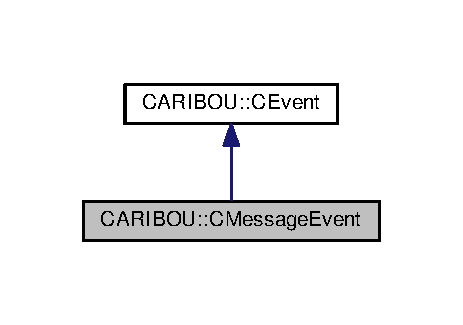
\includegraphics[width=222pt]{class_c_a_r_i_b_o_u_1_1_c_message_event__inherit__graph}
\end{center}
\end{figure}


Collaboration diagram for C\-A\-R\-I\-B\-O\-U\-:\-:C\-Message\-Event\-:\nopagebreak
\begin{figure}[H]
\begin{center}
\leavevmode
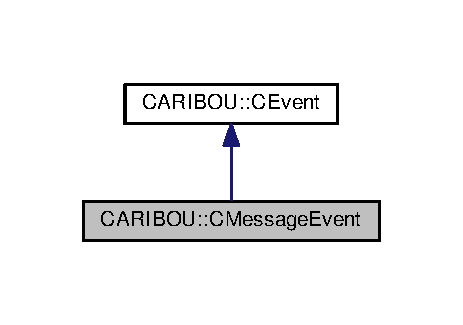
\includegraphics[width=222pt]{class_c_a_r_i_b_o_u_1_1_c_message_event__coll__graph}
\end{center}
\end{figure}
\subsection*{Public Member Functions}
\begin{DoxyCompactItemize}
\item 
{\bf C\-Message\-Event} ({\bf C\-Object} $\ast${\bf sender}, void $\ast${\bf msg})
\item 
{\bf C\-Message\-Event} ({\bf C\-Message\-Event} $\ast$other)
\item 
{\bf C\-Message\-Event} ({\bf C\-Message\-Event} \&other)
\item 
virtual {\bf $\sim$\-C\-Message\-Event} ()
\item 
virtual void {\bf copy} ({\bf C\-Message\-Event} \&other)
\item 
void $\ast$ {\bf msg} ()
\end{DoxyCompactItemize}
\subsection*{Additional Inherited Members}


\subsection{Detailed Description}


Definition at line 24 of file cmessageevent.\-h.



\subsection{Constructor \& Destructor Documentation}
\index{C\-A\-R\-I\-B\-O\-U\-::\-C\-Message\-Event@{C\-A\-R\-I\-B\-O\-U\-::\-C\-Message\-Event}!C\-Message\-Event@{C\-Message\-Event}}
\index{C\-Message\-Event@{C\-Message\-Event}!CARIBOU::CMessageEvent@{C\-A\-R\-I\-B\-O\-U\-::\-C\-Message\-Event}}
\subsubsection[{C\-Message\-Event}]{\setlength{\rightskip}{0pt plus 5cm}C\-A\-R\-I\-B\-O\-U\-::\-C\-Message\-Event\-::\-C\-Message\-Event (
\begin{DoxyParamCaption}
\item[{{\bf C\-Object} $\ast$}]{sender, }
\item[{void $\ast$}]{msg}
\end{DoxyParamCaption}
)}\label{class_c_a_r_i_b_o_u_1_1_c_message_event_af5d7f845ac90d1c3fe9fc46e1e17a0dd}


Definition at line 24 of file cmessageevent.\-cpp.

\index{C\-A\-R\-I\-B\-O\-U\-::\-C\-Message\-Event@{C\-A\-R\-I\-B\-O\-U\-::\-C\-Message\-Event}!C\-Message\-Event@{C\-Message\-Event}}
\index{C\-Message\-Event@{C\-Message\-Event}!CARIBOU::CMessageEvent@{C\-A\-R\-I\-B\-O\-U\-::\-C\-Message\-Event}}
\subsubsection[{C\-Message\-Event}]{\setlength{\rightskip}{0pt plus 5cm}C\-A\-R\-I\-B\-O\-U\-::\-C\-Message\-Event\-::\-C\-Message\-Event (
\begin{DoxyParamCaption}
\item[{{\bf C\-Message\-Event} $\ast$}]{other}
\end{DoxyParamCaption}
)\hspace{0.3cm}{\ttfamily [inline]}}\label{class_c_a_r_i_b_o_u_1_1_c_message_event_a77eeaf43b1a4e903ffc81427dbdf6779}


Definition at line 28 of file cmessageevent.\-h.

\index{C\-A\-R\-I\-B\-O\-U\-::\-C\-Message\-Event@{C\-A\-R\-I\-B\-O\-U\-::\-C\-Message\-Event}!C\-Message\-Event@{C\-Message\-Event}}
\index{C\-Message\-Event@{C\-Message\-Event}!CARIBOU::CMessageEvent@{C\-A\-R\-I\-B\-O\-U\-::\-C\-Message\-Event}}
\subsubsection[{C\-Message\-Event}]{\setlength{\rightskip}{0pt plus 5cm}C\-A\-R\-I\-B\-O\-U\-::\-C\-Message\-Event\-::\-C\-Message\-Event (
\begin{DoxyParamCaption}
\item[{{\bf C\-Message\-Event} \&}]{other}
\end{DoxyParamCaption}
)\hspace{0.3cm}{\ttfamily [inline]}}\label{class_c_a_r_i_b_o_u_1_1_c_message_event_aa28b6742795f121f6690b764768df067}


Definition at line 29 of file cmessageevent.\-h.

\index{C\-A\-R\-I\-B\-O\-U\-::\-C\-Message\-Event@{C\-A\-R\-I\-B\-O\-U\-::\-C\-Message\-Event}!$\sim$\-C\-Message\-Event@{$\sim$\-C\-Message\-Event}}
\index{$\sim$\-C\-Message\-Event@{$\sim$\-C\-Message\-Event}!CARIBOU::CMessageEvent@{C\-A\-R\-I\-B\-O\-U\-::\-C\-Message\-Event}}
\subsubsection[{$\sim$\-C\-Message\-Event}]{\setlength{\rightskip}{0pt plus 5cm}C\-A\-R\-I\-B\-O\-U\-::\-C\-Message\-Event\-::$\sim$\-C\-Message\-Event (
\begin{DoxyParamCaption}
{}
\end{DoxyParamCaption}
)\hspace{0.3cm}{\ttfamily [virtual]}}\label{class_c_a_r_i_b_o_u_1_1_c_message_event_a28ca761cd9351b48b4f4e0879622e63f}


Definition at line 31 of file cmessageevent.\-cpp.



\subsection{Member Function Documentation}
\index{C\-A\-R\-I\-B\-O\-U\-::\-C\-Message\-Event@{C\-A\-R\-I\-B\-O\-U\-::\-C\-Message\-Event}!copy@{copy}}
\index{copy@{copy}!CARIBOU::CMessageEvent@{C\-A\-R\-I\-B\-O\-U\-::\-C\-Message\-Event}}
\subsubsection[{copy}]{\setlength{\rightskip}{0pt plus 5cm}void C\-A\-R\-I\-B\-O\-U\-::\-C\-Message\-Event\-::copy (
\begin{DoxyParamCaption}
\item[{{\bf C\-Message\-Event} \&}]{other}
\end{DoxyParamCaption}
)\hspace{0.3cm}{\ttfamily [virtual]}}\label{class_c_a_r_i_b_o_u_1_1_c_message_event_a433a23a9cf7ef849b8779c0aefa1271f}


Definition at line 35 of file cmessageevent.\-cpp.

\index{C\-A\-R\-I\-B\-O\-U\-::\-C\-Message\-Event@{C\-A\-R\-I\-B\-O\-U\-::\-C\-Message\-Event}!msg@{msg}}
\index{msg@{msg}!CARIBOU::CMessageEvent@{C\-A\-R\-I\-B\-O\-U\-::\-C\-Message\-Event}}
\subsubsection[{msg}]{\setlength{\rightskip}{0pt plus 5cm}void$\ast$ C\-A\-R\-I\-B\-O\-U\-::\-C\-Message\-Event\-::msg (
\begin{DoxyParamCaption}
{}
\end{DoxyParamCaption}
)\hspace{0.3cm}{\ttfamily [inline]}}\label{class_c_a_r_i_b_o_u_1_1_c_message_event_a2b1254029044407e02a5a9cb6d58207e}


Definition at line 33 of file cmessageevent.\-h.



The documentation for this class was generated from the following files\-:\begin{DoxyCompactItemize}
\item 
include/caribou++/{\bf cmessageevent.\-h}\item 
src/{\bf cmessageevent.\-cpp}\end{DoxyCompactItemize}

\section{C\+A\+R\+I\+B\+OU\+:\+:C\+Mutex Class Reference}
\label{class_c_a_r_i_b_o_u_1_1_c_mutex}\index{C\+A\+R\+I\+B\+O\+U\+::\+C\+Mutex@{C\+A\+R\+I\+B\+O\+U\+::\+C\+Mutex}}


Implements a mutex data structure.  




{\ttfamily \#include $<$cmutex.\+h$>$}

\subsection*{Public Member Functions}
\begin{DoxyCompactItemize}
\item 
{\bf C\+Mutex} (uint8\+\_\+t {\bf flags}=0, bool {\bf lock}=false)
\item 
{\bf $\sim$\+C\+Mutex} ()
\item 
bool {\bf try\+Lock} ()
\begin{DoxyCompactList}\small\item\em Test the lock, and return true if it was acquired. \end{DoxyCompactList}\item 
bool {\bf lock} (int timeout=0)
\begin{DoxyCompactList}\small\item\em Sleep while acquiring the lock. \end{DoxyCompactList}\item 
bool {\bf unlock} ()
\begin{DoxyCompactList}\small\item\em Release a previously acquired lock. \end{DoxyCompactList}\item 
uint16\+\_\+t {\bf locks} ()
\begin{DoxyCompactList}\small\item\em Return the number of locks held. \end{DoxyCompactList}\item 
uint8\+\_\+t {\bf flags} ()
\item 
void {\bf set\+Flags} (uint8\+\_\+t {\bf flags})
\end{DoxyCompactItemize}


\subsection{Detailed Description}
Implements a mutex data structure. 

\begin{DoxyAuthor}{Author}
Michael Sharkey {\tt mike@pikeaero.\+com} 
\end{DoxyAuthor}


Definition at line 28 of file cmutex.\+h.



\subsection{Constructor \& Destructor Documentation}
\index{C\+A\+R\+I\+B\+O\+U\+::\+C\+Mutex@{C\+A\+R\+I\+B\+O\+U\+::\+C\+Mutex}!C\+Mutex@{C\+Mutex}}
\index{C\+Mutex@{C\+Mutex}!C\+A\+R\+I\+B\+O\+U\+::\+C\+Mutex@{C\+A\+R\+I\+B\+O\+U\+::\+C\+Mutex}}
\subsubsection[{C\+Mutex(uint8\+\_\+t flags=0, bool lock=false)}]{\setlength{\rightskip}{0pt plus 5cm}C\+A\+R\+I\+B\+O\+U\+::\+C\+Mutex\+::\+C\+Mutex (
\begin{DoxyParamCaption}
\item[{uint8\+\_\+t}]{flags = {\ttfamily 0}, }
\item[{bool}]{lock = {\ttfamily false}}
\end{DoxyParamCaption}
)}\label{class_c_a_r_i_b_o_u_1_1_c_mutex_a45cfc863c038e329c85a2982e33e256f}


Definition at line 21 of file cmutex.\+cpp.

\index{C\+A\+R\+I\+B\+O\+U\+::\+C\+Mutex@{C\+A\+R\+I\+B\+O\+U\+::\+C\+Mutex}!````~C\+Mutex@{$\sim$\+C\+Mutex}}
\index{````~C\+Mutex@{$\sim$\+C\+Mutex}!C\+A\+R\+I\+B\+O\+U\+::\+C\+Mutex@{C\+A\+R\+I\+B\+O\+U\+::\+C\+Mutex}}
\subsubsection[{$\sim$\+C\+Mutex()}]{\setlength{\rightskip}{0pt plus 5cm}C\+A\+R\+I\+B\+O\+U\+::\+C\+Mutex\+::$\sim$\+C\+Mutex (
\begin{DoxyParamCaption}
{}
\end{DoxyParamCaption}
)}\label{class_c_a_r_i_b_o_u_1_1_c_mutex_a33f77184619fe1db8faf6a1a65ee3173}


Definition at line 30 of file cmutex.\+cpp.



\subsection{Member Function Documentation}
\index{C\+A\+R\+I\+B\+O\+U\+::\+C\+Mutex@{C\+A\+R\+I\+B\+O\+U\+::\+C\+Mutex}!flags@{flags}}
\index{flags@{flags}!C\+A\+R\+I\+B\+O\+U\+::\+C\+Mutex@{C\+A\+R\+I\+B\+O\+U\+::\+C\+Mutex}}
\subsubsection[{flags()}]{\setlength{\rightskip}{0pt plus 5cm}uint8\+\_\+t C\+A\+R\+I\+B\+O\+U\+::\+C\+Mutex\+::flags (
\begin{DoxyParamCaption}
{}
\end{DoxyParamCaption}
)}\label{class_c_a_r_i_b_o_u_1_1_c_mutex_abe0e8feff1b1398c38acdf3a637c4d7e}


Definition at line 59 of file cmutex.\+cpp.

\index{C\+A\+R\+I\+B\+O\+U\+::\+C\+Mutex@{C\+A\+R\+I\+B\+O\+U\+::\+C\+Mutex}!lock@{lock}}
\index{lock@{lock}!C\+A\+R\+I\+B\+O\+U\+::\+C\+Mutex@{C\+A\+R\+I\+B\+O\+U\+::\+C\+Mutex}}
\subsubsection[{lock(int timeout=0)}]{\setlength{\rightskip}{0pt plus 5cm}bool C\+A\+R\+I\+B\+O\+U\+::\+C\+Mutex\+::lock (
\begin{DoxyParamCaption}
\item[{int}]{timeout = {\ttfamily 0}}
\end{DoxyParamCaption}
)}\label{class_c_a_r_i_b_o_u_1_1_c_mutex_a8150905f7bf1985f20800b1c2ed90009}


Sleep while acquiring the lock. 



Definition at line 41 of file cmutex.\+cpp.

\index{C\+A\+R\+I\+B\+O\+U\+::\+C\+Mutex@{C\+A\+R\+I\+B\+O\+U\+::\+C\+Mutex}!locks@{locks}}
\index{locks@{locks}!C\+A\+R\+I\+B\+O\+U\+::\+C\+Mutex@{C\+A\+R\+I\+B\+O\+U\+::\+C\+Mutex}}
\subsubsection[{locks()}]{\setlength{\rightskip}{0pt plus 5cm}uint16\+\_\+t C\+A\+R\+I\+B\+O\+U\+::\+C\+Mutex\+::locks (
\begin{DoxyParamCaption}
{}
\end{DoxyParamCaption}
)}\label{class_c_a_r_i_b_o_u_1_1_c_mutex_a39a3b7a3f2ca22451733f78c97be11cb}


Return the number of locks held. 



Definition at line 53 of file cmutex.\+cpp.

\index{C\+A\+R\+I\+B\+O\+U\+::\+C\+Mutex@{C\+A\+R\+I\+B\+O\+U\+::\+C\+Mutex}!set\+Flags@{set\+Flags}}
\index{set\+Flags@{set\+Flags}!C\+A\+R\+I\+B\+O\+U\+::\+C\+Mutex@{C\+A\+R\+I\+B\+O\+U\+::\+C\+Mutex}}
\subsubsection[{set\+Flags(uint8\+\_\+t flags)}]{\setlength{\rightskip}{0pt plus 5cm}void C\+A\+R\+I\+B\+O\+U\+::\+C\+Mutex\+::set\+Flags (
\begin{DoxyParamCaption}
\item[{uint8\+\_\+t}]{flags}
\end{DoxyParamCaption}
)}\label{class_c_a_r_i_b_o_u_1_1_c_mutex_a1b7906abef38d09edfa1d7597eb029f3}


Definition at line 65 of file cmutex.\+cpp.

\index{C\+A\+R\+I\+B\+O\+U\+::\+C\+Mutex@{C\+A\+R\+I\+B\+O\+U\+::\+C\+Mutex}!try\+Lock@{try\+Lock}}
\index{try\+Lock@{try\+Lock}!C\+A\+R\+I\+B\+O\+U\+::\+C\+Mutex@{C\+A\+R\+I\+B\+O\+U\+::\+C\+Mutex}}
\subsubsection[{try\+Lock()}]{\setlength{\rightskip}{0pt plus 5cm}bool C\+A\+R\+I\+B\+O\+U\+::\+C\+Mutex\+::try\+Lock (
\begin{DoxyParamCaption}
{}
\end{DoxyParamCaption}
)}\label{class_c_a_r_i_b_o_u_1_1_c_mutex_aa860d6d2b7ced801a0fa52c13962a799}


Test the lock, and return true if it was acquired. 



Definition at line 35 of file cmutex.\+cpp.

\index{C\+A\+R\+I\+B\+O\+U\+::\+C\+Mutex@{C\+A\+R\+I\+B\+O\+U\+::\+C\+Mutex}!unlock@{unlock}}
\index{unlock@{unlock}!C\+A\+R\+I\+B\+O\+U\+::\+C\+Mutex@{C\+A\+R\+I\+B\+O\+U\+::\+C\+Mutex}}
\subsubsection[{unlock()}]{\setlength{\rightskip}{0pt plus 5cm}bool C\+A\+R\+I\+B\+O\+U\+::\+C\+Mutex\+::unlock (
\begin{DoxyParamCaption}
{}
\end{DoxyParamCaption}
)}\label{class_c_a_r_i_b_o_u_1_1_c_mutex_adf3e045a757ed5b11ef1d19f70cded04}


Release a previously acquired lock. 



Definition at line 47 of file cmutex.\+cpp.



The documentation for this class was generated from the following files\+:\begin{DoxyCompactItemize}
\item 
include/caribou++/{\bf cmutex.\+h}\item 
src/{\bf cmutex.\+cpp}\end{DoxyCompactItemize}

\section{C\-A\-R\-I\-B\-O\-U\-:\-:C\-Mutex\-Locker Class Reference}
\label{class_c_a_r_i_b_o_u_1_1_c_mutex_locker}\index{C\-A\-R\-I\-B\-O\-U\-::\-C\-Mutex\-Locker@{C\-A\-R\-I\-B\-O\-U\-::\-C\-Mutex\-Locker}}


{\ttfamily \#include $<$cmutexlocker.\-h$>$}

\subsection*{Public Member Functions}
\begin{DoxyCompactItemize}
\item 
{\bf C\-Mutex\-Locker} ({\bf C\-Mutex} \&mutex)
\item 
{\bf C\-Mutex\-Locker} ({\bf C\-Mutex} $\ast$mutex)
\item 
{\bf $\sim$\-C\-Mutex\-Locker} ()
\end{DoxyCompactItemize}


\subsection{Detailed Description}
\begin{DoxyAuthor}{Author}
Michael Sharkey {\tt mike@pikeaero.\-com} 
\end{DoxyAuthor}


Definition at line 28 of file cmutexlocker.\-h.



\subsection{Constructor \& Destructor Documentation}
\index{C\-A\-R\-I\-B\-O\-U\-::\-C\-Mutex\-Locker@{C\-A\-R\-I\-B\-O\-U\-::\-C\-Mutex\-Locker}!C\-Mutex\-Locker@{C\-Mutex\-Locker}}
\index{C\-Mutex\-Locker@{C\-Mutex\-Locker}!CARIBOU::CMutexLocker@{C\-A\-R\-I\-B\-O\-U\-::\-C\-Mutex\-Locker}}
\subsubsection[{C\-Mutex\-Locker}]{\setlength{\rightskip}{0pt plus 5cm}C\-A\-R\-I\-B\-O\-U\-::\-C\-Mutex\-Locker\-::\-C\-Mutex\-Locker (
\begin{DoxyParamCaption}
\item[{{\bf C\-Mutex} \&}]{mutex}
\end{DoxyParamCaption}
)}\label{class_c_a_r_i_b_o_u_1_1_c_mutex_locker_a0aa1199d2b11a0235c985083f65c00bc}


Definition at line 21 of file cmutexlocker.\-cpp.

\index{C\-A\-R\-I\-B\-O\-U\-::\-C\-Mutex\-Locker@{C\-A\-R\-I\-B\-O\-U\-::\-C\-Mutex\-Locker}!C\-Mutex\-Locker@{C\-Mutex\-Locker}}
\index{C\-Mutex\-Locker@{C\-Mutex\-Locker}!CARIBOU::CMutexLocker@{C\-A\-R\-I\-B\-O\-U\-::\-C\-Mutex\-Locker}}
\subsubsection[{C\-Mutex\-Locker}]{\setlength{\rightskip}{0pt plus 5cm}C\-A\-R\-I\-B\-O\-U\-::\-C\-Mutex\-Locker\-::\-C\-Mutex\-Locker (
\begin{DoxyParamCaption}
\item[{{\bf C\-Mutex} $\ast$}]{mutex}
\end{DoxyParamCaption}
)}\label{class_c_a_r_i_b_o_u_1_1_c_mutex_locker_a82983541841ae6df867dfb1599a74c29}


Definition at line 27 of file cmutexlocker.\-cpp.

\index{C\-A\-R\-I\-B\-O\-U\-::\-C\-Mutex\-Locker@{C\-A\-R\-I\-B\-O\-U\-::\-C\-Mutex\-Locker}!$\sim$\-C\-Mutex\-Locker@{$\sim$\-C\-Mutex\-Locker}}
\index{$\sim$\-C\-Mutex\-Locker@{$\sim$\-C\-Mutex\-Locker}!CARIBOU::CMutexLocker@{C\-A\-R\-I\-B\-O\-U\-::\-C\-Mutex\-Locker}}
\subsubsection[{$\sim$\-C\-Mutex\-Locker}]{\setlength{\rightskip}{0pt plus 5cm}C\-A\-R\-I\-B\-O\-U\-::\-C\-Mutex\-Locker\-::$\sim$\-C\-Mutex\-Locker (
\begin{DoxyParamCaption}
{}
\end{DoxyParamCaption}
)}\label{class_c_a_r_i_b_o_u_1_1_c_mutex_locker_a5856c05ca57948199b180ad9e763e2df}


Definition at line 33 of file cmutexlocker.\-cpp.



The documentation for this class was generated from the following files\-:\begin{DoxyCompactItemize}
\item 
include/caribou++/{\bf cmutexlocker.\-h}\item 
src/{\bf cmutexlocker.\-cpp}\end{DoxyCompactItemize}

\section{C\+A\+R\+I\+B\+OU\+:\+:C\+Object Class Reference}
\label{class_c_a_r_i_b_o_u_1_1_c_object}\index{C\+A\+R\+I\+B\+O\+U\+::\+C\+Object@{C\+A\+R\+I\+B\+O\+U\+::\+C\+Object}}


{\ttfamily \#include $<$cobject.\+h$>$}



Inheritance diagram for C\+A\+R\+I\+B\+OU\+:\+:C\+Object\+:
\nopagebreak
\begin{figure}[H]
\begin{center}
\leavevmode
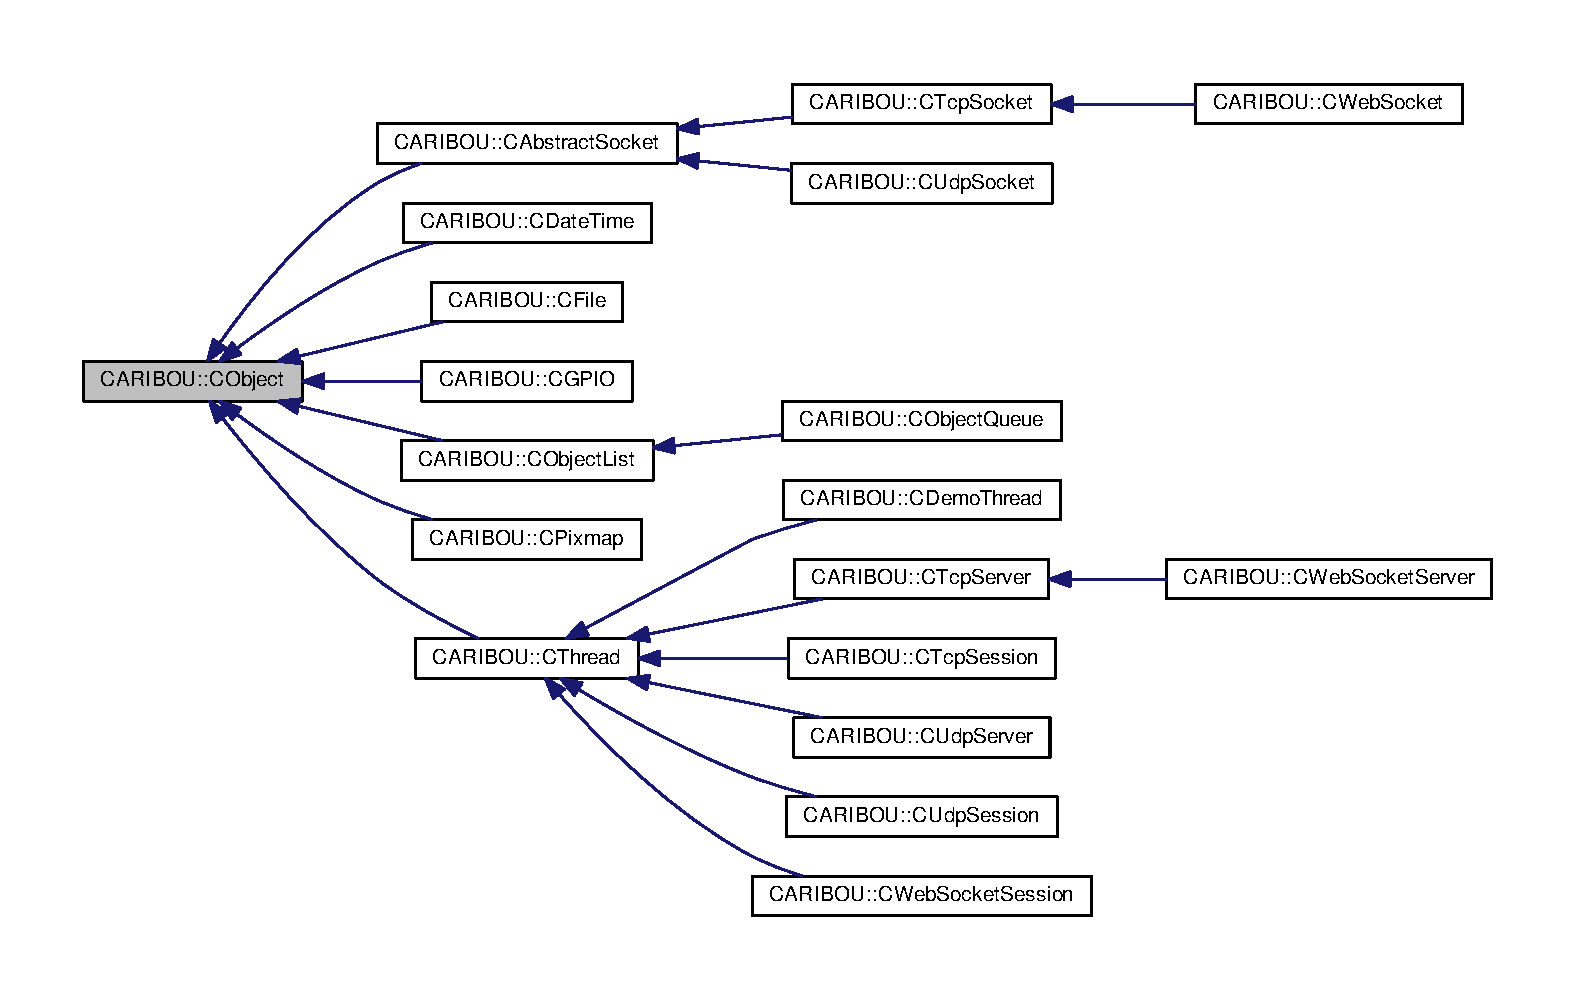
\includegraphics[width=350pt]{class_c_a_r_i_b_o_u_1_1_c_object__inherit__graph}
\end{center}
\end{figure}
\subsection*{Public Types}
\begin{DoxyCompactItemize}
\item 
enum {\bf t\+Error\+Code} \{ {\bf err\+OK} = 0, 
{\bf err\+Out\+Of\+Memory} = 100, 
{\bf err\+Out\+Of\+Range}, 
{\bf err\+Timeout}
 \}
\end{DoxyCompactItemize}
\subsection*{Public Member Functions}
\begin{DoxyCompactItemize}
\item 
{\bf C\+Object} ()
\item 
virtual {\bf $\sim$\+C\+Object} ()
\item 
uint16\+\_\+t {\bf obj\+Class} ()
\item 
void {\bf broadcast} ({\bf C\+Event} $\ast$e)
\begin{DoxyCompactList}\small\item\em broadcast an event to anyone listening. \end{DoxyCompactList}\item 
void {\bf timer\+Callback} ({\bf C\+Timer\+Event} $\ast$e)
\begin{DoxyCompactList}\small\item\em Do not call this method directly. Used for \doxyref{C\+A\+R\+I\+B\+OU}{p.}{namespace_c_a_r_i_b_o_u} thread timer callback. \end{DoxyCompactList}\item 
void {\bf public\+\_\+irq} (Interrupt\+Vector vector)
\end{DoxyCompactItemize}
\subsection*{Static Public Member Functions}
\begin{DoxyCompactItemize}
\item 
static void {\bf reset} ()
\item 
static void {\bf \+\_\+isr} (Interrupt\+Vector vector)
\begin{DoxyCompactList}\small\item\em Executes a Hardware Reset. \end{DoxyCompactList}\item 
static int {\bf disable\+Vector} (Interrupt\+Vector vector)
\begin{DoxyCompactList}\small\item\em set interrupt vector mask -\/ disabling interrupts to that vector. \end{DoxyCompactList}\item 
static int {\bf enable\+Vector} (Interrupt\+Vector vector)
\begin{DoxyCompactList}\small\item\em clear interrupt vector mask -\/ enables interrupts to that vector. \end{DoxyCompactList}\item 
static int {\bf vector\+Enabled} (Interrupt\+Vector vector)
\item 
static int {\bf vector\+Set\+Enabled} (Interrupt\+Vector vector, int state)
\item 
static bool {\bf install\+Vector\+I\+RQ} (Interrupt\+Vector vector, {\bf C\+Object} $\ast$object)
\begin{DoxyCompactList}\small\item\em Install an I\+RQ interrupt handler object at an interrupt vector. \end{DoxyCompactList}\item 
static bool {\bf remove\+Vector\+I\+RQ} (Interrupt\+Vector vector, {\bf C\+Object} $\ast$object)
\begin{DoxyCompactList}\small\item\em Remove an specific I\+RQ interrupt handler object by it\textquotesingle{}s C\+Object$\ast$ pointer. \end{DoxyCompactList}\item 
static bool {\bf remove\+Vector\+I\+RQ} ({\bf C\+Object} $\ast$object)
\begin{DoxyCompactList}\small\item\em Remove an I\+RQ interrupt handler object by it\textquotesingle{}s C\+Object$\ast$ pointer. \end{DoxyCompactList}\item 
static void {\bf install\+Listener} ({\bf C\+Object} $\ast$object, int type)
\begin{DoxyCompactList}\small\item\em install an event listener \end{DoxyCompactList}\item 
static void {\bf remove\+Listener} ({\bf C\+Object} $\ast$object, int type)
\begin{DoxyCompactList}\small\item\em remove an event listener \end{DoxyCompactList}\item 
static bool {\bf object\+Lock} ()
\item 
static bool {\bf object\+Unlock} ()
\item 
static {\bf C\+A\+R\+I\+B\+O\+U\+::\+C\+Mutex} \& {\bf object\+Mutex} ()
\end{DoxyCompactItemize}
\subsection*{Protected Member Functions}
\begin{DoxyCompactItemize}
\item 
virtual void {\bf irq} (Interrupt\+Vector vector)
\begin{DoxyCompactList}\small\item\em receive a hardware interrupt. \end{DoxyCompactList}\item 
virtual void {\bf event} ({\bf C\+Event} $\ast$e)
\begin{DoxyCompactList}\small\item\em receive a queued event, the complement of \doxyref{C\+Object\+::dispatch(\+C\+Event$\ast$)}{p.}{class_c_a_r_i_b_o_u_1_1_c_object_a8aa02620cb58d4e2d3e19999aa0fbfe7}. \end{DoxyCompactList}\item 
virtual caribou\+\_\+timer\+\_\+t $\ast$ {\bf start\+Timer} (uint32\+\_\+t msec)
\begin{DoxyCompactList}\small\item\em Start a new timer belonging to this object. \end{DoxyCompactList}\item 
virtual caribou\+\_\+timer\+\_\+t $\ast$ {\bf reset\+Timer} (caribou\+\_\+timer\+\_\+t $\ast$timer\+Id)
\begin{DoxyCompactList}\small\item\em Restart an existing timer belonging to this object. \end{DoxyCompactList}\item 
virtual void {\bf kill\+Timer} (caribou\+\_\+timer\+\_\+t $\ast$timer\+Id)
\begin{DoxyCompactList}\small\item\em stop a timer and remove it from the queueu \end{DoxyCompactList}\end{DoxyCompactItemize}
\subsection*{Static Protected Member Functions}
\begin{DoxyCompactItemize}
\item 
static void {\bf periodic} ()
\begin{DoxyCompactList}\small\item\em perform periodic queue maintenance \end{DoxyCompactList}\item 
static int {\bf purge} ({\bf C\+Object} $\ast$object)
\begin{DoxyCompactList}\small\item\em purge all references to the specified object from the listener map. \end{DoxyCompactList}\item 
static bool {\bf enqueue} ({\bf C\+Event} $\ast$e)
\begin{DoxyCompactList}\small\item\em Enqueue an event for later dispatch. \end{DoxyCompactList}\item 
static void {\bf dequeue} ()
\begin{DoxyCompactList}\small\item\em dispatch some events in the current task\textquotesingle{}s time slice \end{DoxyCompactList}\item 
static void {\bf dispatch} ({\bf C\+Event} $\ast$e)
\begin{DoxyCompactList}\small\item\em dispatch a particular event registered listener object\textquotesingle{}s event(...) method. \end{DoxyCompactList}\end{DoxyCompactItemize}
\subsection*{Protected Attributes}
\begin{DoxyCompactItemize}
\item 
uint16\+\_\+t {\bf m\+Obj\+Class}
\end{DoxyCompactItemize}
\subsection*{Friends}
\begin{DoxyCompactItemize}
\item 
class {\bf C\+Caribou\+Main\+Thread}
\item 
void {\bf isr\+\_\+vector} (Interrupt\+Vector vector, void $\ast${\bf arg})
\end{DoxyCompactItemize}


\subsection{Detailed Description}


Definition at line 35 of file cobject.\+h.



\subsection{Member Enumeration Documentation}
\index{C\+A\+R\+I\+B\+O\+U\+::\+C\+Object@{C\+A\+R\+I\+B\+O\+U\+::\+C\+Object}!t\+Error\+Code@{t\+Error\+Code}}
\index{t\+Error\+Code@{t\+Error\+Code}!C\+A\+R\+I\+B\+O\+U\+::\+C\+Object@{C\+A\+R\+I\+B\+O\+U\+::\+C\+Object}}
\subsubsection[{t\+Error\+Code}]{\setlength{\rightskip}{0pt plus 5cm}enum {\bf C\+A\+R\+I\+B\+O\+U\+::\+C\+Object\+::t\+Error\+Code}}\label{class_c_a_r_i_b_o_u_1_1_c_object_ada6f2c3bc1871ff029c875c4fa9bff2d}
\begin{Desc}
\item[Enumerator]\par
\begin{description}
\index{err\+OK@{err\+OK}!C\+A\+R\+I\+B\+O\+U\+::\+C\+Object@{C\+A\+R\+I\+B\+O\+U\+::\+C\+Object}}\index{C\+A\+R\+I\+B\+O\+U\+::\+C\+Object@{C\+A\+R\+I\+B\+O\+U\+::\+C\+Object}!err\+OK@{err\+OK}}\item[{\em 
err\+OK\label{class_c_a_r_i_b_o_u_1_1_c_object_ada6f2c3bc1871ff029c875c4fa9bff2daecf3a54669809642cfdea153f00063ba}
}]\index{err\+Out\+Of\+Memory@{err\+Out\+Of\+Memory}!C\+A\+R\+I\+B\+O\+U\+::\+C\+Object@{C\+A\+R\+I\+B\+O\+U\+::\+C\+Object}}\index{C\+A\+R\+I\+B\+O\+U\+::\+C\+Object@{C\+A\+R\+I\+B\+O\+U\+::\+C\+Object}!err\+Out\+Of\+Memory@{err\+Out\+Of\+Memory}}\item[{\em 
err\+Out\+Of\+Memory\label{class_c_a_r_i_b_o_u_1_1_c_object_ada6f2c3bc1871ff029c875c4fa9bff2da17334cbc664a56113ce5193fc610f6d0}
}]\index{err\+Out\+Of\+Range@{err\+Out\+Of\+Range}!C\+A\+R\+I\+B\+O\+U\+::\+C\+Object@{C\+A\+R\+I\+B\+O\+U\+::\+C\+Object}}\index{C\+A\+R\+I\+B\+O\+U\+::\+C\+Object@{C\+A\+R\+I\+B\+O\+U\+::\+C\+Object}!err\+Out\+Of\+Range@{err\+Out\+Of\+Range}}\item[{\em 
err\+Out\+Of\+Range\label{class_c_a_r_i_b_o_u_1_1_c_object_ada6f2c3bc1871ff029c875c4fa9bff2da500563dd3d21bdd5caa746687805d619}
}]\index{err\+Timeout@{err\+Timeout}!C\+A\+R\+I\+B\+O\+U\+::\+C\+Object@{C\+A\+R\+I\+B\+O\+U\+::\+C\+Object}}\index{C\+A\+R\+I\+B\+O\+U\+::\+C\+Object@{C\+A\+R\+I\+B\+O\+U\+::\+C\+Object}!err\+Timeout@{err\+Timeout}}\item[{\em 
err\+Timeout\label{class_c_a_r_i_b_o_u_1_1_c_object_ada6f2c3bc1871ff029c875c4fa9bff2da73675a1505e413c7bc586a38ac36e55a}
}]\end{description}
\end{Desc}


Definition at line 40 of file cobject.\+h.



\subsection{Constructor \& Destructor Documentation}
\index{C\+A\+R\+I\+B\+O\+U\+::\+C\+Object@{C\+A\+R\+I\+B\+O\+U\+::\+C\+Object}!C\+Object@{C\+Object}}
\index{C\+Object@{C\+Object}!C\+A\+R\+I\+B\+O\+U\+::\+C\+Object@{C\+A\+R\+I\+B\+O\+U\+::\+C\+Object}}
\subsubsection[{C\+Object()}]{\setlength{\rightskip}{0pt plus 5cm}C\+A\+R\+I\+B\+O\+U\+::\+C\+Object\+::\+C\+Object (
\begin{DoxyParamCaption}
{}
\end{DoxyParamCaption}
)}\label{class_c_a_r_i_b_o_u_1_1_c_object_a4f245c634385d254173761b7181010b6}


Definition at line 63 of file cobject.\+cpp.

\index{C\+A\+R\+I\+B\+O\+U\+::\+C\+Object@{C\+A\+R\+I\+B\+O\+U\+::\+C\+Object}!````~C\+Object@{$\sim$\+C\+Object}}
\index{````~C\+Object@{$\sim$\+C\+Object}!C\+A\+R\+I\+B\+O\+U\+::\+C\+Object@{C\+A\+R\+I\+B\+O\+U\+::\+C\+Object}}
\subsubsection[{$\sim$\+C\+Object()}]{\setlength{\rightskip}{0pt plus 5cm}C\+A\+R\+I\+B\+O\+U\+::\+C\+Object\+::$\sim$\+C\+Object (
\begin{DoxyParamCaption}
{}
\end{DoxyParamCaption}
)\hspace{0.3cm}{\ttfamily [virtual]}}\label{class_c_a_r_i_b_o_u_1_1_c_object_a95c0f3da92003bf3ccf7a5b38f9c5a21}


Definition at line 68 of file cobject.\+cpp.



\subsection{Member Function Documentation}
\index{C\+A\+R\+I\+B\+O\+U\+::\+C\+Object@{C\+A\+R\+I\+B\+O\+U\+::\+C\+Object}!\+\_\+isr@{\+\_\+isr}}
\index{\+\_\+isr@{\+\_\+isr}!C\+A\+R\+I\+B\+O\+U\+::\+C\+Object@{C\+A\+R\+I\+B\+O\+U\+::\+C\+Object}}
\subsubsection[{\+\_\+isr(\+Interrupt\+Vector vector)}]{\setlength{\rightskip}{0pt plus 5cm}static void C\+A\+R\+I\+B\+O\+U\+::\+C\+Object\+::\+\_\+isr (
\begin{DoxyParamCaption}
\item[{Interrupt\+Vector}]{vector}
\end{DoxyParamCaption}
)\hspace{0.3cm}{\ttfamily [static]}}\label{class_c_a_r_i_b_o_u_1_1_c_object_a604c17d9721e6d844bf39d3b2392d7cf}


Executes a Hardware Reset. 

Interrupt vector operations... \index{C\+A\+R\+I\+B\+O\+U\+::\+C\+Object@{C\+A\+R\+I\+B\+O\+U\+::\+C\+Object}!broadcast@{broadcast}}
\index{broadcast@{broadcast}!C\+A\+R\+I\+B\+O\+U\+::\+C\+Object@{C\+A\+R\+I\+B\+O\+U\+::\+C\+Object}}
\subsubsection[{broadcast(\+C\+Event $\ast$e)}]{\setlength{\rightskip}{0pt plus 5cm}void C\+A\+R\+I\+B\+O\+U\+::\+C\+Object\+::broadcast (
\begin{DoxyParamCaption}
\item[{{\bf C\+Event} $\ast$}]{e}
\end{DoxyParamCaption}
)}\label{class_c_a_r_i_b_o_u_1_1_c_object_af63e3f2435599f4ad6106f06796f271e}


broadcast an event to anyone listening. 

The event is queued to be sent out at a later time. This is the prefered method of message delivery.

Queued type of dispatch. 
\begin{DoxyParams}{Parameters}
{\em e} & The event to dispatch. \\
\hline
\end{DoxyParams}


Definition at line 92 of file cobject.\+cpp.

\index{C\+A\+R\+I\+B\+O\+U\+::\+C\+Object@{C\+A\+R\+I\+B\+O\+U\+::\+C\+Object}!dequeue@{dequeue}}
\index{dequeue@{dequeue}!C\+A\+R\+I\+B\+O\+U\+::\+C\+Object@{C\+A\+R\+I\+B\+O\+U\+::\+C\+Object}}
\subsubsection[{dequeue()}]{\setlength{\rightskip}{0pt plus 5cm}void C\+A\+R\+I\+B\+O\+U\+::\+C\+Object\+::dequeue (
\begin{DoxyParamCaption}
{}
\end{DoxyParamCaption}
)\hspace{0.3cm}{\ttfamily [static]}, {\ttfamily [protected]}}\label{class_c_a_r_i_b_o_u_1_1_c_object_a764dd30657bb07ccbd9faa2074288156}


dispatch some events in the current task\textquotesingle{}s time slice 



Definition at line 228 of file cobject.\+cpp.

\index{C\+A\+R\+I\+B\+O\+U\+::\+C\+Object@{C\+A\+R\+I\+B\+O\+U\+::\+C\+Object}!disable\+Vector@{disable\+Vector}}
\index{disable\+Vector@{disable\+Vector}!C\+A\+R\+I\+B\+O\+U\+::\+C\+Object@{C\+A\+R\+I\+B\+O\+U\+::\+C\+Object}}
\subsubsection[{disable\+Vector(\+Interrupt\+Vector vector)}]{\setlength{\rightskip}{0pt plus 5cm}int C\+A\+R\+I\+B\+O\+U\+::\+C\+Object\+::disable\+Vector (
\begin{DoxyParamCaption}
\item[{Interrupt\+Vector}]{vector}
\end{DoxyParamCaption}
)\hspace{0.3cm}{\ttfamily [static]}}\label{class_c_a_r_i_b_o_u_1_1_c_object_a768fec44b695bede808a56f6ea3505a0}


set interrupt vector mask -\/ disabling interrupts to that vector. 



Definition at line 159 of file cobject.\+cpp.

\index{C\+A\+R\+I\+B\+O\+U\+::\+C\+Object@{C\+A\+R\+I\+B\+O\+U\+::\+C\+Object}!dispatch@{dispatch}}
\index{dispatch@{dispatch}!C\+A\+R\+I\+B\+O\+U\+::\+C\+Object@{C\+A\+R\+I\+B\+O\+U\+::\+C\+Object}}
\subsubsection[{dispatch(\+C\+Event $\ast$e)}]{\setlength{\rightskip}{0pt plus 5cm}void C\+A\+R\+I\+B\+O\+U\+::\+C\+Object\+::dispatch (
\begin{DoxyParamCaption}
\item[{{\bf C\+Event} $\ast$}]{e}
\end{DoxyParamCaption}
)\hspace{0.3cm}{\ttfamily [static]}, {\ttfamily [protected]}}\label{class_c_a_r_i_b_o_u_1_1_c_object_a8aa02620cb58d4e2d3e19999aa0fbfe7}


dispatch a particular event registered listener object\textquotesingle{}s event(...) method. 


\begin{DoxyParams}{Parameters}
{\em e} & The event to dispatch must already be detached from the event queue. \\
\hline
\end{DoxyParams}
\begin{DoxyNote}{Note}
dispatch(...) owns the pointer. 

Thread locks are used to guard the listener map. This implies that the listening object should not use a M\+U\+T\+EX while receiving the event in order to avoid a deadlock condition. 
\end{DoxyNote}
Then we delete the event object... 

Definition at line 276 of file cobject.\+cpp.

\index{C\+A\+R\+I\+B\+O\+U\+::\+C\+Object@{C\+A\+R\+I\+B\+O\+U\+::\+C\+Object}!enable\+Vector@{enable\+Vector}}
\index{enable\+Vector@{enable\+Vector}!C\+A\+R\+I\+B\+O\+U\+::\+C\+Object@{C\+A\+R\+I\+B\+O\+U\+::\+C\+Object}}
\subsubsection[{enable\+Vector(\+Interrupt\+Vector vector)}]{\setlength{\rightskip}{0pt plus 5cm}int C\+A\+R\+I\+B\+O\+U\+::\+C\+Object\+::enable\+Vector (
\begin{DoxyParamCaption}
\item[{Interrupt\+Vector}]{vector}
\end{DoxyParamCaption}
)\hspace{0.3cm}{\ttfamily [static]}}\label{class_c_a_r_i_b_o_u_1_1_c_object_a42cdb13c7718ca65eece9e7d37044713}


clear interrupt vector mask -\/ enables interrupts to that vector. 



Definition at line 151 of file cobject.\+cpp.

\index{C\+A\+R\+I\+B\+O\+U\+::\+C\+Object@{C\+A\+R\+I\+B\+O\+U\+::\+C\+Object}!enqueue@{enqueue}}
\index{enqueue@{enqueue}!C\+A\+R\+I\+B\+O\+U\+::\+C\+Object@{C\+A\+R\+I\+B\+O\+U\+::\+C\+Object}}
\subsubsection[{enqueue(\+C\+Event $\ast$e)}]{\setlength{\rightskip}{0pt plus 5cm}bool C\+A\+R\+I\+B\+O\+U\+::\+C\+Object\+::enqueue (
\begin{DoxyParamCaption}
\item[{{\bf C\+Event} $\ast$}]{e}
\end{DoxyParamCaption}
)\hspace{0.3cm}{\ttfamily [static]}, {\ttfamily [protected]}}\label{class_c_a_r_i_b_o_u_1_1_c_object_aa2b90aa47d543ec190ce882faef5a075}


Enqueue an event for later dispatch. 

C\+Event\+Queue has event ownership and will delete it unless e-\/$>$sender\+Owns() is true. \begin{DoxyReturn}{Returns}
true if the event was queued. 
\end{DoxyReturn}
Only enqueue the event if somebody is listening to it\textquotesingle{}s type...

jump the queue -\/ L\+I\+FO mode

T\+O\+DO -\/ load testing required. test threshold where flooding hi priority events begins to starve the queue.

normal/low priority -\/ F\+I\+FO mode. 

Definition at line 247 of file cobject.\+cpp.

\index{C\+A\+R\+I\+B\+O\+U\+::\+C\+Object@{C\+A\+R\+I\+B\+O\+U\+::\+C\+Object}!event@{event}}
\index{event@{event}!C\+A\+R\+I\+B\+O\+U\+::\+C\+Object@{C\+A\+R\+I\+B\+O\+U\+::\+C\+Object}}
\subsubsection[{event(\+C\+Event $\ast$e)}]{\setlength{\rightskip}{0pt plus 5cm}void C\+A\+R\+I\+B\+O\+U\+::\+C\+Object\+::event (
\begin{DoxyParamCaption}
\item[{{\bf C\+Event} $\ast$}]{e}
\end{DoxyParamCaption}
)\hspace{0.3cm}{\ttfamily [protected]}, {\ttfamily [virtual]}}\label{class_c_a_r_i_b_o_u_1_1_c_object_a3e0d51872e9834666d064c716340bbdd}


receive a queued event, the complement of \doxyref{C\+Object\+::dispatch(\+C\+Event$\ast$)}{p.}{class_c_a_r_i_b_o_u_1_1_c_object_a8aa02620cb58d4e2d3e19999aa0fbfe7}. 

Process Events. 

Reimplemented in {\bf C\+A\+R\+I\+B\+O\+U\+::\+C\+Date\+Time} \doxyref{}{p.}{class_c_a_r_i_b_o_u_1_1_c_date_time_a35c1d14db0523c8da5748ca2b8245bed}, {\bf C\+A\+R\+I\+B\+O\+U\+::\+C\+G\+P\+IO} \doxyref{}{p.}{class_c_a_r_i_b_o_u_1_1_c_g_p_i_o_ab67320903fc92646816756ab6507be12}, and {\bf C\+A\+R\+I\+B\+O\+U\+::\+C\+Demo\+Thread} \doxyref{}{p.}{class_c_a_r_i_b_o_u_1_1_c_demo_thread_a28c300137fb5433552299575036eddc6}.



Definition at line 144 of file cobject.\+cpp.

\index{C\+A\+R\+I\+B\+O\+U\+::\+C\+Object@{C\+A\+R\+I\+B\+O\+U\+::\+C\+Object}!install\+Listener@{install\+Listener}}
\index{install\+Listener@{install\+Listener}!C\+A\+R\+I\+B\+O\+U\+::\+C\+Object@{C\+A\+R\+I\+B\+O\+U\+::\+C\+Object}}
\subsubsection[{install\+Listener(\+C\+Object $\ast$object, int type)}]{\setlength{\rightskip}{0pt plus 5cm}void C\+A\+R\+I\+B\+O\+U\+::\+C\+Object\+::install\+Listener (
\begin{DoxyParamCaption}
\item[{{\bf C\+Object} $\ast$}]{object, }
\item[{int}]{type}
\end{DoxyParamCaption}
)\hspace{0.3cm}{\ttfamily [static]}}\label{class_c_a_r_i_b_o_u_1_1_c_object_aa3d6d893a87d14a29193407e74356a1e}


install an event listener 



Definition at line 209 of file cobject.\+cpp.

\index{C\+A\+R\+I\+B\+O\+U\+::\+C\+Object@{C\+A\+R\+I\+B\+O\+U\+::\+C\+Object}!install\+Vector\+I\+RQ@{install\+Vector\+I\+RQ}}
\index{install\+Vector\+I\+RQ@{install\+Vector\+I\+RQ}!C\+A\+R\+I\+B\+O\+U\+::\+C\+Object@{C\+A\+R\+I\+B\+O\+U\+::\+C\+Object}}
\subsubsection[{install\+Vector\+I\+R\+Q(\+Interrupt\+Vector vector, C\+Object $\ast$object)}]{\setlength{\rightskip}{0pt plus 5cm}bool C\+A\+R\+I\+B\+O\+U\+::\+C\+Object\+::install\+Vector\+I\+RQ (
\begin{DoxyParamCaption}
\item[{Interrupt\+Vector}]{vector, }
\item[{{\bf C\+Object} $\ast$}]{object}
\end{DoxyParamCaption}
)\hspace{0.3cm}{\ttfamily [static]}}\label{class_c_a_r_i_b_o_u_1_1_c_object_afe6dfd5bf95e56b4d5f31c1253b3ec7a}


Install an I\+RQ interrupt handler object at an interrupt vector. 


\begin{DoxyParams}{Parameters}
{\em vector} & The vector number 0-\/63 \\
\hline
{\em object} & The object to recieve the interrupt. \\
\hline
\end{DoxyParams}
\begin{DoxyReturn}{Returns}
boolean 
\end{DoxyReturn}


Definition at line 180 of file cobject.\+cpp.

\index{C\+A\+R\+I\+B\+O\+U\+::\+C\+Object@{C\+A\+R\+I\+B\+O\+U\+::\+C\+Object}!irq@{irq}}
\index{irq@{irq}!C\+A\+R\+I\+B\+O\+U\+::\+C\+Object@{C\+A\+R\+I\+B\+O\+U\+::\+C\+Object}}
\subsubsection[{irq(\+Interrupt\+Vector vector)}]{\setlength{\rightskip}{0pt plus 5cm}virtual void C\+A\+R\+I\+B\+O\+U\+::\+C\+Object\+::irq (
\begin{DoxyParamCaption}
\item[{Interrupt\+Vector}]{vector}
\end{DoxyParamCaption}
)\hspace{0.3cm}{\ttfamily [inline]}, {\ttfamily [protected]}, {\ttfamily [virtual]}}\label{class_c_a_r_i_b_o_u_1_1_c_object_a5552bc7421bdc00f7142657b4c77659d}


receive a hardware interrupt. 

If this object has register itself as in interrupt handler using install\+Vector\+I\+RQ(...) for a particular vector. This interrupts will come in through this method. 

Definition at line 97 of file cobject.\+h.

\index{C\+A\+R\+I\+B\+O\+U\+::\+C\+Object@{C\+A\+R\+I\+B\+O\+U\+::\+C\+Object}!kill\+Timer@{kill\+Timer}}
\index{kill\+Timer@{kill\+Timer}!C\+A\+R\+I\+B\+O\+U\+::\+C\+Object@{C\+A\+R\+I\+B\+O\+U\+::\+C\+Object}}
\subsubsection[{kill\+Timer(caribou\+\_\+timer\+\_\+t $\ast$timer\+Id)}]{\setlength{\rightskip}{0pt plus 5cm}void C\+A\+R\+I\+B\+O\+U\+::\+C\+Object\+::kill\+Timer (
\begin{DoxyParamCaption}
\item[{caribou\+\_\+timer\+\_\+t $\ast$}]{timer\+Id}
\end{DoxyParamCaption}
)\hspace{0.3cm}{\ttfamily [protected]}, {\ttfamily [virtual]}}\label{class_c_a_r_i_b_o_u_1_1_c_object_ace22c3f5d89d76a244ce8768ac5915ec}


stop a timer and remove it from the queueu 


\begin{DoxyParams}{Parameters}
{\em id} & The timer id as returned from \doxyref{start\+Timer()}{p.}{class_c_a_r_i_b_o_u_1_1_c_object_a161c595e752ef2c9c020b1eba2472751} \\
\hline
\end{DoxyParams}


Definition at line 128 of file cobject.\+cpp.

\index{C\+A\+R\+I\+B\+O\+U\+::\+C\+Object@{C\+A\+R\+I\+B\+O\+U\+::\+C\+Object}!obj\+Class@{obj\+Class}}
\index{obj\+Class@{obj\+Class}!C\+A\+R\+I\+B\+O\+U\+::\+C\+Object@{C\+A\+R\+I\+B\+O\+U\+::\+C\+Object}}
\subsubsection[{obj\+Class()}]{\setlength{\rightskip}{0pt plus 5cm}uint16\+\_\+t C\+A\+R\+I\+B\+O\+U\+::\+C\+Object\+::obj\+Class (
\begin{DoxyParamCaption}
{}
\end{DoxyParamCaption}
)\hspace{0.3cm}{\ttfamily [inline]}}\label{class_c_a_r_i_b_o_u_1_1_c_object_ac8d07a0958771151e7003a03a0830945}


Definition at line 50 of file cobject.\+h.

\index{C\+A\+R\+I\+B\+O\+U\+::\+C\+Object@{C\+A\+R\+I\+B\+O\+U\+::\+C\+Object}!object\+Lock@{object\+Lock}}
\index{object\+Lock@{object\+Lock}!C\+A\+R\+I\+B\+O\+U\+::\+C\+Object@{C\+A\+R\+I\+B\+O\+U\+::\+C\+Object}}
\subsubsection[{object\+Lock()}]{\setlength{\rightskip}{0pt plus 5cm}bool C\+A\+R\+I\+B\+O\+U\+::\+C\+Object\+::object\+Lock (
\begin{DoxyParamCaption}
{}
\end{DoxyParamCaption}
)\hspace{0.3cm}{\ttfamily [static]}}\label{class_c_a_r_i_b_o_u_1_1_c_object_a821bbb79c9b19ab535414f109fec15bb}


Definition at line 73 of file cobject.\+cpp.

\index{C\+A\+R\+I\+B\+O\+U\+::\+C\+Object@{C\+A\+R\+I\+B\+O\+U\+::\+C\+Object}!object\+Mutex@{object\+Mutex}}
\index{object\+Mutex@{object\+Mutex}!C\+A\+R\+I\+B\+O\+U\+::\+C\+Object@{C\+A\+R\+I\+B\+O\+U\+::\+C\+Object}}
\subsubsection[{object\+Mutex()}]{\setlength{\rightskip}{0pt plus 5cm}{\bf C\+A\+R\+I\+B\+O\+U\+::\+C\+Mutex} \& C\+A\+R\+I\+B\+O\+U\+::\+C\+Object\+::object\+Mutex (
\begin{DoxyParamCaption}
{}
\end{DoxyParamCaption}
)\hspace{0.3cm}{\ttfamily [static]}}\label{class_c_a_r_i_b_o_u_1_1_c_object_a99d95d2e0e50cfcc450b4acd428e44c3}


Definition at line 83 of file cobject.\+cpp.

\index{C\+A\+R\+I\+B\+O\+U\+::\+C\+Object@{C\+A\+R\+I\+B\+O\+U\+::\+C\+Object}!object\+Unlock@{object\+Unlock}}
\index{object\+Unlock@{object\+Unlock}!C\+A\+R\+I\+B\+O\+U\+::\+C\+Object@{C\+A\+R\+I\+B\+O\+U\+::\+C\+Object}}
\subsubsection[{object\+Unlock()}]{\setlength{\rightskip}{0pt plus 5cm}bool C\+A\+R\+I\+B\+O\+U\+::\+C\+Object\+::object\+Unlock (
\begin{DoxyParamCaption}
{}
\end{DoxyParamCaption}
)\hspace{0.3cm}{\ttfamily [static]}}\label{class_c_a_r_i_b_o_u_1_1_c_object_a21a33420977901d3fc0295ace46b75eb}


Definition at line 78 of file cobject.\+cpp.

\index{C\+A\+R\+I\+B\+O\+U\+::\+C\+Object@{C\+A\+R\+I\+B\+O\+U\+::\+C\+Object}!periodic@{periodic}}
\index{periodic@{periodic}!C\+A\+R\+I\+B\+O\+U\+::\+C\+Object@{C\+A\+R\+I\+B\+O\+U\+::\+C\+Object}}
\subsubsection[{periodic()}]{\setlength{\rightskip}{0pt plus 5cm}void C\+A\+R\+I\+B\+O\+U\+::\+C\+Object\+::periodic (
\begin{DoxyParamCaption}
{}
\end{DoxyParamCaption}
)\hspace{0.3cm}{\ttfamily [static]}, {\ttfamily [protected]}}\label{class_c_a_r_i_b_o_u_1_1_c_object_af6912a27c8a17cf190ca9eecb378e0b1}


perform periodic queue maintenance 



Definition at line 333 of file cobject.\+cpp.

\index{C\+A\+R\+I\+B\+O\+U\+::\+C\+Object@{C\+A\+R\+I\+B\+O\+U\+::\+C\+Object}!public\+\_\+irq@{public\+\_\+irq}}
\index{public\+\_\+irq@{public\+\_\+irq}!C\+A\+R\+I\+B\+O\+U\+::\+C\+Object@{C\+A\+R\+I\+B\+O\+U\+::\+C\+Object}}
\subsubsection[{public\+\_\+irq(\+Interrupt\+Vector vector)}]{\setlength{\rightskip}{0pt plus 5cm}void C\+A\+R\+I\+B\+O\+U\+::\+C\+Object\+::public\+\_\+irq (
\begin{DoxyParamCaption}
\item[{Interrupt\+Vector}]{vector}
\end{DoxyParamCaption}
)\hspace{0.3cm}{\ttfamily [inline]}}\label{class_c_a_r_i_b_o_u_1_1_c_object_aabc21ec01134dac0d5f783ef8e59fa22}


Definition at line 78 of file cobject.\+h.

\index{C\+A\+R\+I\+B\+O\+U\+::\+C\+Object@{C\+A\+R\+I\+B\+O\+U\+::\+C\+Object}!purge@{purge}}
\index{purge@{purge}!C\+A\+R\+I\+B\+O\+U\+::\+C\+Object@{C\+A\+R\+I\+B\+O\+U\+::\+C\+Object}}
\subsubsection[{purge(\+C\+Object $\ast$object)}]{\setlength{\rightskip}{0pt plus 5cm}int C\+A\+R\+I\+B\+O\+U\+::\+C\+Object\+::purge (
\begin{DoxyParamCaption}
\item[{{\bf C\+Object} $\ast$}]{object}
\end{DoxyParamCaption}
)\hspace{0.3cm}{\ttfamily [static]}, {\ttfamily [protected]}}\label{class_c_a_r_i_b_o_u_1_1_c_object_ac676cf946070f7a95fbea560fc961bb6}


purge all references to the specified object from the listener map. 

If there are any events in the queue that are addressed to or from the object, then remove them...

Definition at line 302 of file cobject.\+cpp.

\index{C\+A\+R\+I\+B\+O\+U\+::\+C\+Object@{C\+A\+R\+I\+B\+O\+U\+::\+C\+Object}!remove\+Listener@{remove\+Listener}}
\index{remove\+Listener@{remove\+Listener}!C\+A\+R\+I\+B\+O\+U\+::\+C\+Object@{C\+A\+R\+I\+B\+O\+U\+::\+C\+Object}}
\subsubsection[{remove\+Listener(\+C\+Object $\ast$object, int type)}]{\setlength{\rightskip}{0pt plus 5cm}void C\+A\+R\+I\+B\+O\+U\+::\+C\+Object\+::remove\+Listener (
\begin{DoxyParamCaption}
\item[{{\bf C\+Object} $\ast$}]{object, }
\item[{int}]{type}
\end{DoxyParamCaption}
)\hspace{0.3cm}{\ttfamily [static]}}\label{class_c_a_r_i_b_o_u_1_1_c_object_a06c025cfc96f8bf91ed9e95da4113eb7}


remove an event listener 



Definition at line 218 of file cobject.\+cpp.

\index{C\+A\+R\+I\+B\+O\+U\+::\+C\+Object@{C\+A\+R\+I\+B\+O\+U\+::\+C\+Object}!remove\+Vector\+I\+RQ@{remove\+Vector\+I\+RQ}}
\index{remove\+Vector\+I\+RQ@{remove\+Vector\+I\+RQ}!C\+A\+R\+I\+B\+O\+U\+::\+C\+Object@{C\+A\+R\+I\+B\+O\+U\+::\+C\+Object}}
\subsubsection[{remove\+Vector\+I\+R\+Q(\+Interrupt\+Vector vector, C\+Object $\ast$object)}]{\setlength{\rightskip}{0pt plus 5cm}bool C\+A\+R\+I\+B\+O\+U\+::\+C\+Object\+::remove\+Vector\+I\+RQ (
\begin{DoxyParamCaption}
\item[{Interrupt\+Vector}]{vector, }
\item[{{\bf C\+Object} $\ast$}]{object}
\end{DoxyParamCaption}
)\hspace{0.3cm}{\ttfamily [static]}}\label{class_c_a_r_i_b_o_u_1_1_c_object_a9e6a2dcb77c28391d193ef9c7824c17f}


Remove an specific I\+RQ interrupt handler object by it\textquotesingle{}s C\+Object$\ast$ pointer. 


\begin{DoxyParams}{Parameters}
{\em object} & The object to recieve the interrupt. \\
\hline
\end{DoxyParams}
\begin{DoxyReturn}{Returns}
boolean 
\end{DoxyReturn}


Definition at line 191 of file cobject.\+cpp.

\index{C\+A\+R\+I\+B\+O\+U\+::\+C\+Object@{C\+A\+R\+I\+B\+O\+U\+::\+C\+Object}!remove\+Vector\+I\+RQ@{remove\+Vector\+I\+RQ}}
\index{remove\+Vector\+I\+RQ@{remove\+Vector\+I\+RQ}!C\+A\+R\+I\+B\+O\+U\+::\+C\+Object@{C\+A\+R\+I\+B\+O\+U\+::\+C\+Object}}
\subsubsection[{remove\+Vector\+I\+R\+Q(\+C\+Object $\ast$object)}]{\setlength{\rightskip}{0pt plus 5cm}bool C\+A\+R\+I\+B\+O\+U\+::\+C\+Object\+::remove\+Vector\+I\+RQ (
\begin{DoxyParamCaption}
\item[{{\bf C\+Object} $\ast$}]{object}
\end{DoxyParamCaption}
)\hspace{0.3cm}{\ttfamily [static]}}\label{class_c_a_r_i_b_o_u_1_1_c_object_aaca14dad99b56fefe79c29e814e8a7e1}


Remove an I\+RQ interrupt handler object by it\textquotesingle{}s C\+Object$\ast$ pointer. 


\begin{DoxyParams}{Parameters}
{\em object} & The object to recieve the interrupt. \\
\hline
\end{DoxyParams}
\begin{DoxyReturn}{Returns}
boolean 
\end{DoxyReturn}


Definition at line 202 of file cobject.\+cpp.

\index{C\+A\+R\+I\+B\+O\+U\+::\+C\+Object@{C\+A\+R\+I\+B\+O\+U\+::\+C\+Object}!reset@{reset}}
\index{reset@{reset}!C\+A\+R\+I\+B\+O\+U\+::\+C\+Object@{C\+A\+R\+I\+B\+O\+U\+::\+C\+Object}}
\subsubsection[{reset()}]{\setlength{\rightskip}{0pt plus 5cm}static void C\+A\+R\+I\+B\+O\+U\+::\+C\+Object\+::reset (
\begin{DoxyParamCaption}
{}
\end{DoxyParamCaption}
)\hspace{0.3cm}{\ttfamily [static]}}\label{class_c_a_r_i_b_o_u_1_1_c_object_afd7e4165ffee627fcc28ab06e7c1e82a}
\index{C\+A\+R\+I\+B\+O\+U\+::\+C\+Object@{C\+A\+R\+I\+B\+O\+U\+::\+C\+Object}!reset\+Timer@{reset\+Timer}}
\index{reset\+Timer@{reset\+Timer}!C\+A\+R\+I\+B\+O\+U\+::\+C\+Object@{C\+A\+R\+I\+B\+O\+U\+::\+C\+Object}}
\subsubsection[{reset\+Timer(caribou\+\_\+timer\+\_\+t $\ast$timer\+Id)}]{\setlength{\rightskip}{0pt plus 5cm}caribou\+\_\+timer\+\_\+t $\ast$ C\+A\+R\+I\+B\+O\+U\+::\+C\+Object\+::reset\+Timer (
\begin{DoxyParamCaption}
\item[{caribou\+\_\+timer\+\_\+t $\ast$}]{timer\+Id}
\end{DoxyParamCaption}
)\hspace{0.3cm}{\ttfamily [protected]}, {\ttfamily [virtual]}}\label{class_c_a_r_i_b_o_u_1_1_c_object_a4348f9ae493c94d3236b48727ad30b90}


Restart an existing timer belonging to this object. 

The timer will emit \doxyref{C\+Timer\+Event}{p.}{class_c_a_r_i_b_o_u_1_1_c_timer_event} objects to the \doxyref{C\+Object\+::event(\+C\+Event$\ast$)}{p.}{class_c_a_r_i_b_o_u_1_1_c_object_a3e0d51872e9834666d064c716340bbdd} method at the prescribed intervals. 
\begin{DoxyParams}{Parameters}
{\em msec} & the number of milliseonds until the timer expires. \\
\hline
\end{DoxyParams}
\begin{DoxyReturn}{Returns}
a unique identifier. 
\end{DoxyReturn}


Definition at line 118 of file cobject.\+cpp.

\index{C\+A\+R\+I\+B\+O\+U\+::\+C\+Object@{C\+A\+R\+I\+B\+O\+U\+::\+C\+Object}!start\+Timer@{start\+Timer}}
\index{start\+Timer@{start\+Timer}!C\+A\+R\+I\+B\+O\+U\+::\+C\+Object@{C\+A\+R\+I\+B\+O\+U\+::\+C\+Object}}
\subsubsection[{start\+Timer(uint32\+\_\+t msec)}]{\setlength{\rightskip}{0pt plus 5cm}caribou\+\_\+timer\+\_\+t $\ast$ C\+A\+R\+I\+B\+O\+U\+::\+C\+Object\+::start\+Timer (
\begin{DoxyParamCaption}
\item[{uint32\+\_\+t}]{msec}
\end{DoxyParamCaption}
)\hspace{0.3cm}{\ttfamily [protected]}, {\ttfamily [virtual]}}\label{class_c_a_r_i_b_o_u_1_1_c_object_a161c595e752ef2c9c020b1eba2472751}


Start a new timer belonging to this object. 

The timer will emit \doxyref{C\+Timer\+Event}{p.}{class_c_a_r_i_b_o_u_1_1_c_timer_event} objects to the \doxyref{C\+Object\+::event(\+C\+Event$\ast$)}{p.}{class_c_a_r_i_b_o_u_1_1_c_object_a3e0d51872e9834666d064c716340bbdd} method at the prescribed intervals. 
\begin{DoxyParams}{Parameters}
{\em msec} & the number of milliseonds until the timer expires. \\
\hline
\end{DoxyParams}
\begin{DoxyReturn}{Returns}
a unique identifier (id). 
\end{DoxyReturn}


Definition at line 104 of file cobject.\+cpp.

\index{C\+A\+R\+I\+B\+O\+U\+::\+C\+Object@{C\+A\+R\+I\+B\+O\+U\+::\+C\+Object}!timer\+Callback@{timer\+Callback}}
\index{timer\+Callback@{timer\+Callback}!C\+A\+R\+I\+B\+O\+U\+::\+C\+Object@{C\+A\+R\+I\+B\+O\+U\+::\+C\+Object}}
\subsubsection[{timer\+Callback(\+C\+Timer\+Event $\ast$e)}]{\setlength{\rightskip}{0pt plus 5cm}void C\+A\+R\+I\+B\+O\+U\+::\+C\+Object\+::timer\+Callback (
\begin{DoxyParamCaption}
\item[{{\bf C\+Timer\+Event} $\ast$}]{e}
\end{DoxyParamCaption}
)}\label{class_c_a_r_i_b_o_u_1_1_c_object_ac4943fbc7ce7bc0ada92038208c439cf}


Do not call this method directly. Used for \doxyref{C\+A\+R\+I\+B\+OU}{p.}{namespace_c_a_r_i_b_o_u} thread timer callback. 

get here on a timer event callback 

Definition at line 136 of file cobject.\+cpp.

\index{C\+A\+R\+I\+B\+O\+U\+::\+C\+Object@{C\+A\+R\+I\+B\+O\+U\+::\+C\+Object}!vector\+Enabled@{vector\+Enabled}}
\index{vector\+Enabled@{vector\+Enabled}!C\+A\+R\+I\+B\+O\+U\+::\+C\+Object@{C\+A\+R\+I\+B\+O\+U\+::\+C\+Object}}
\subsubsection[{vector\+Enabled(\+Interrupt\+Vector vector)}]{\setlength{\rightskip}{0pt plus 5cm}int C\+A\+R\+I\+B\+O\+U\+::\+C\+Object\+::vector\+Enabled (
\begin{DoxyParamCaption}
\item[{Interrupt\+Vector}]{vector}
\end{DoxyParamCaption}
)\hspace{0.3cm}{\ttfamily [static]}}\label{class_c_a_r_i_b_o_u_1_1_c_object_a4528b159ba0274336d90d62fddc8c917}


Definition at line 164 of file cobject.\+cpp.

\index{C\+A\+R\+I\+B\+O\+U\+::\+C\+Object@{C\+A\+R\+I\+B\+O\+U\+::\+C\+Object}!vector\+Set\+Enabled@{vector\+Set\+Enabled}}
\index{vector\+Set\+Enabled@{vector\+Set\+Enabled}!C\+A\+R\+I\+B\+O\+U\+::\+C\+Object@{C\+A\+R\+I\+B\+O\+U\+::\+C\+Object}}
\subsubsection[{vector\+Set\+Enabled(\+Interrupt\+Vector vector, int state)}]{\setlength{\rightskip}{0pt plus 5cm}int C\+A\+R\+I\+B\+O\+U\+::\+C\+Object\+::vector\+Set\+Enabled (
\begin{DoxyParamCaption}
\item[{Interrupt\+Vector}]{vector, }
\item[{int}]{state}
\end{DoxyParamCaption}
)\hspace{0.3cm}{\ttfamily [static]}}\label{class_c_a_r_i_b_o_u_1_1_c_object_abee2a6efc821643094818abd33441c56}


Definition at line 169 of file cobject.\+cpp.



\subsection{Friends And Related Function Documentation}
\index{C\+A\+R\+I\+B\+O\+U\+::\+C\+Object@{C\+A\+R\+I\+B\+O\+U\+::\+C\+Object}!C\+Caribou\+Main\+Thread@{C\+Caribou\+Main\+Thread}}
\index{C\+Caribou\+Main\+Thread@{C\+Caribou\+Main\+Thread}!C\+A\+R\+I\+B\+O\+U\+::\+C\+Object@{C\+A\+R\+I\+B\+O\+U\+::\+C\+Object}}
\subsubsection[{C\+Caribou\+Main\+Thread}]{\setlength{\rightskip}{0pt plus 5cm}friend class {\bf C\+Caribou\+Main\+Thread}\hspace{0.3cm}{\ttfamily [friend]}}\label{class_c_a_r_i_b_o_u_1_1_c_object_a57b1331e02ed7977c46fcf03b21e42b3}


Definition at line 38 of file cobject.\+h.

\index{C\+A\+R\+I\+B\+O\+U\+::\+C\+Object@{C\+A\+R\+I\+B\+O\+U\+::\+C\+Object}!isr\+\_\+vector@{isr\+\_\+vector}}
\index{isr\+\_\+vector@{isr\+\_\+vector}!C\+A\+R\+I\+B\+O\+U\+::\+C\+Object@{C\+A\+R\+I\+B\+O\+U\+::\+C\+Object}}
\subsubsection[{isr\+\_\+vector}]{\setlength{\rightskip}{0pt plus 5cm}void isr\+\_\+vector (
\begin{DoxyParamCaption}
\item[{Interrupt\+Vector}]{vector, }
\item[{void $\ast$}]{arg}
\end{DoxyParamCaption}
)\hspace{0.3cm}{\ttfamily [friend]}}\label{class_c_a_r_i_b_o_u_1_1_c_object_a91cfbaf2f9458196dab71287b2c00be4}


Definition at line 33 of file cobject.\+cpp.



\subsection{Member Data Documentation}
\index{C\+A\+R\+I\+B\+O\+U\+::\+C\+Object@{C\+A\+R\+I\+B\+O\+U\+::\+C\+Object}!m\+Obj\+Class@{m\+Obj\+Class}}
\index{m\+Obj\+Class@{m\+Obj\+Class}!C\+A\+R\+I\+B\+O\+U\+::\+C\+Object@{C\+A\+R\+I\+B\+O\+U\+::\+C\+Object}}
\subsubsection[{m\+Obj\+Class}]{\setlength{\rightskip}{0pt plus 5cm}uint16\+\_\+t C\+A\+R\+I\+B\+O\+U\+::\+C\+Object\+::m\+Obj\+Class\hspace{0.3cm}{\ttfamily [protected]}}\label{class_c_a_r_i_b_o_u_1_1_c_object_a11b3f435986119e79fa4b21212e419d5}


Definition at line 89 of file cobject.\+h.



The documentation for this class was generated from the following files\+:\begin{DoxyCompactItemize}
\item 
include/caribou++/{\bf cobject.\+h}\item 
src/{\bf cobject.\+cpp}\end{DoxyCompactItemize}

\section{C\+A\+R\+I\+B\+OU\+:\+:C\+Object\+List Class Reference}
\label{class_c_a_r_i_b_o_u_1_1_c_object_list}\index{C\+A\+R\+I\+B\+O\+U\+::\+C\+Object\+List@{C\+A\+R\+I\+B\+O\+U\+::\+C\+Object\+List}}


Implements a list of object pointers.  




{\ttfamily \#include $<$cobjectlist.\+h$>$}



Inheritance diagram for C\+A\+R\+I\+B\+OU\+:\+:C\+Object\+List\+:
\nopagebreak
\begin{figure}[H]
\begin{center}
\leavevmode
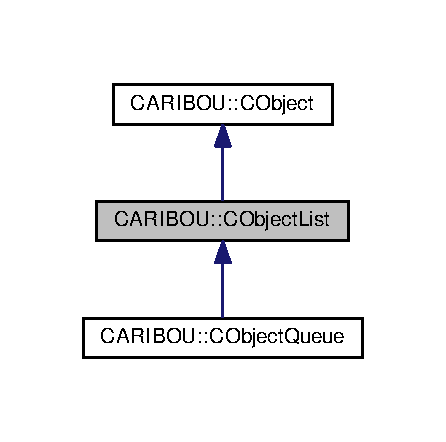
\includegraphics[width=214pt]{class_c_a_r_i_b_o_u_1_1_c_object_list__inherit__graph}
\end{center}
\end{figure}


Collaboration diagram for C\+A\+R\+I\+B\+OU\+:\+:C\+Object\+List\+:\nopagebreak
\begin{figure}[H]
\begin{center}
\leavevmode
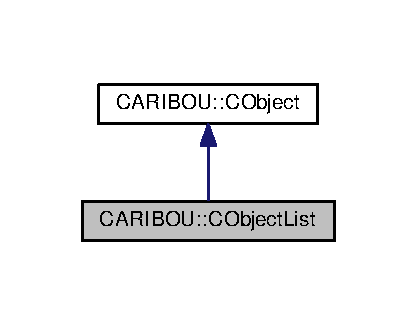
\includegraphics[width=201pt]{class_c_a_r_i_b_o_u_1_1_c_object_list__coll__graph}
\end{center}
\end{figure}
\subsection*{Public Member Functions}
\begin{DoxyCompactItemize}
\item 
{\bf C\+Object\+List} ()
\begin{DoxyCompactList}\small\item\em T\+O\+DO -\/ make these list classes templace classes. \end{DoxyCompactList}\item 
{\bf C\+Object\+List} (size\+\_\+t size)
\item 
{\bf $\sim$\+C\+Object\+List} ()
\item 
virtual {\bf C\+Object\+List} \& {\bf append} (const {\bf C\+Object} $\ast$object)
\begin{DoxyCompactList}\small\item\em Append an object to the list. \end{DoxyCompactList}\item 
virtual {\bf C\+Object\+List} \& {\bf remove} (int i)
\begin{DoxyCompactList}\small\item\em Remove an object from the list. \end{DoxyCompactList}\item 
virtual {\bf C\+Object\+List} \& {\bf remove} (const {\bf C\+Object} $\ast$object)
\begin{DoxyCompactList}\small\item\em Remove an object from the list. \end{DoxyCompactList}\item 
virtual {\bf C\+Object\+List} \& {\bf insert} (const {\bf C\+Object} $\ast$object, int32\+\_\+t pos)
\begin{DoxyCompactList}\small\item\em Insert an object into the list. \end{DoxyCompactList}\item 
virtual {\bf C\+Object\+List} \& {\bf resize} (size\+\_\+t size)
\begin{DoxyCompactList}\small\item\em Resize and fill void with null. \end{DoxyCompactList}\item 
{\bf C\+Object\+List} \& {\bf operator+=} (const {\bf C\+Object} $\ast$object)
\item 
{\bf C\+Object\+List} \& {\bf operator-\/=} (const {\bf C\+Object} $\ast$object)
\item 
{\bf C\+Object} $\ast$ {\bf operator[$\,$]} (int n)
\item 
int32\+\_\+t {\bf index\+Of} (const {\bf C\+Object} $\ast$object)
\begin{DoxyCompactList}\small\item\em find an object by pointer value and return it\textquotesingle{}s index \end{DoxyCompactList}\item 
uint32\+\_\+t {\bf count} ()
\item 
{\bf C\+Object} $\ast$ {\bf at} (uint32\+\_\+t n)
\item 
void {\bf set} (uint32\+\_\+t n, {\bf C\+Object} $\ast$obj)
\item 
void {\bf set\+Auto\+Delete} (bool autodelete)
\item 
bool {\bf auto\+Delete} ()
\item 
void {\bf clear} ()
\end{DoxyCompactItemize}
\subsection*{Additional Inherited Members}


\subsection{Detailed Description}
Implements a list of object pointers. 

\begin{DoxyAuthor}{Author}
Michael Sharkey {\tt mike@pikeaero.\+com} 
\end{DoxyAuthor}


Definition at line 28 of file cobjectlist.\+h.



\subsection{Constructor \& Destructor Documentation}
\index{C\+A\+R\+I\+B\+O\+U\+::\+C\+Object\+List@{C\+A\+R\+I\+B\+O\+U\+::\+C\+Object\+List}!C\+Object\+List@{C\+Object\+List}}
\index{C\+Object\+List@{C\+Object\+List}!C\+A\+R\+I\+B\+O\+U\+::\+C\+Object\+List@{C\+A\+R\+I\+B\+O\+U\+::\+C\+Object\+List}}
\subsubsection[{C\+Object\+List()}]{\setlength{\rightskip}{0pt plus 5cm}C\+A\+R\+I\+B\+O\+U\+::\+C\+Object\+List\+::\+C\+Object\+List (
\begin{DoxyParamCaption}
{}
\end{DoxyParamCaption}
)}\label{class_c_a_r_i_b_o_u_1_1_c_object_list_a4ce794d9bbab389c1d68f6b1b25261e7}


T\+O\+DO -\/ make these list classes templace classes. 

T\+O\+DO -\/ use const where applicable T\+O\+DO -\/ test insert at end of list 

Definition at line 22 of file cobjectlist.\+cpp.

\index{C\+A\+R\+I\+B\+O\+U\+::\+C\+Object\+List@{C\+A\+R\+I\+B\+O\+U\+::\+C\+Object\+List}!C\+Object\+List@{C\+Object\+List}}
\index{C\+Object\+List@{C\+Object\+List}!C\+A\+R\+I\+B\+O\+U\+::\+C\+Object\+List@{C\+A\+R\+I\+B\+O\+U\+::\+C\+Object\+List}}
\subsubsection[{C\+Object\+List(size\+\_\+t size)}]{\setlength{\rightskip}{0pt plus 5cm}C\+A\+R\+I\+B\+O\+U\+::\+C\+Object\+List\+::\+C\+Object\+List (
\begin{DoxyParamCaption}
\item[{size\+\_\+t}]{size}
\end{DoxyParamCaption}
)}\label{class_c_a_r_i_b_o_u_1_1_c_object_list_ac1670f5da6165f175f6133df6c41c07c}


Definition at line 31 of file cobjectlist.\+cpp.

\index{C\+A\+R\+I\+B\+O\+U\+::\+C\+Object\+List@{C\+A\+R\+I\+B\+O\+U\+::\+C\+Object\+List}!````~C\+Object\+List@{$\sim$\+C\+Object\+List}}
\index{````~C\+Object\+List@{$\sim$\+C\+Object\+List}!C\+A\+R\+I\+B\+O\+U\+::\+C\+Object\+List@{C\+A\+R\+I\+B\+O\+U\+::\+C\+Object\+List}}
\subsubsection[{$\sim$\+C\+Object\+List()}]{\setlength{\rightskip}{0pt plus 5cm}C\+A\+R\+I\+B\+O\+U\+::\+C\+Object\+List\+::$\sim$\+C\+Object\+List (
\begin{DoxyParamCaption}
{}
\end{DoxyParamCaption}
)}\label{class_c_a_r_i_b_o_u_1_1_c_object_list_a133690b54ddd831aaa1ce22bd8f33f27}


Definition at line 41 of file cobjectlist.\+cpp.



\subsection{Member Function Documentation}
\index{C\+A\+R\+I\+B\+O\+U\+::\+C\+Object\+List@{C\+A\+R\+I\+B\+O\+U\+::\+C\+Object\+List}!append@{append}}
\index{append@{append}!C\+A\+R\+I\+B\+O\+U\+::\+C\+Object\+List@{C\+A\+R\+I\+B\+O\+U\+::\+C\+Object\+List}}
\subsubsection[{append(const C\+Object $\ast$object)}]{\setlength{\rightskip}{0pt plus 5cm}{\bf C\+Object\+List} \& C\+A\+R\+I\+B\+O\+U\+::\+C\+Object\+List\+::append (
\begin{DoxyParamCaption}
\item[{const {\bf C\+Object} $\ast$}]{object}
\end{DoxyParamCaption}
)\hspace{0.3cm}{\ttfamily [virtual]}}\label{class_c_a_r_i_b_o_u_1_1_c_object_list_a23fdc49106c184260c74731f1225e1a1}


Append an object to the list. 



Definition at line 98 of file cobjectlist.\+cpp.

\index{C\+A\+R\+I\+B\+O\+U\+::\+C\+Object\+List@{C\+A\+R\+I\+B\+O\+U\+::\+C\+Object\+List}!at@{at}}
\index{at@{at}!C\+A\+R\+I\+B\+O\+U\+::\+C\+Object\+List@{C\+A\+R\+I\+B\+O\+U\+::\+C\+Object\+List}}
\subsubsection[{at(uint32\+\_\+t n)}]{\setlength{\rightskip}{0pt plus 5cm}{\bf C\+Object} $\ast$ C\+A\+R\+I\+B\+O\+U\+::\+C\+Object\+List\+::at (
\begin{DoxyParamCaption}
\item[{uint32\+\_\+t}]{n}
\end{DoxyParamCaption}
)}\label{class_c_a_r_i_b_o_u_1_1_c_object_list_a9283873c09749727613845d48c612b2b}


Definition at line 62 of file cobjectlist.\+cpp.

\index{C\+A\+R\+I\+B\+O\+U\+::\+C\+Object\+List@{C\+A\+R\+I\+B\+O\+U\+::\+C\+Object\+List}!auto\+Delete@{auto\+Delete}}
\index{auto\+Delete@{auto\+Delete}!C\+A\+R\+I\+B\+O\+U\+::\+C\+Object\+List@{C\+A\+R\+I\+B\+O\+U\+::\+C\+Object\+List}}
\subsubsection[{auto\+Delete()}]{\setlength{\rightskip}{0pt plus 5cm}bool C\+A\+R\+I\+B\+O\+U\+::\+C\+Object\+List\+::auto\+Delete (
\begin{DoxyParamCaption}
{}
\end{DoxyParamCaption}
)\hspace{0.3cm}{\ttfamily [inline]}}\label{class_c_a_r_i_b_o_u_1_1_c_object_list_aa60e45a5e575b4cf694980b9031be197}


Definition at line 54 of file cobjectlist.\+h.

\index{C\+A\+R\+I\+B\+O\+U\+::\+C\+Object\+List@{C\+A\+R\+I\+B\+O\+U\+::\+C\+Object\+List}!clear@{clear}}
\index{clear@{clear}!C\+A\+R\+I\+B\+O\+U\+::\+C\+Object\+List@{C\+A\+R\+I\+B\+O\+U\+::\+C\+Object\+List}}
\subsubsection[{clear()}]{\setlength{\rightskip}{0pt plus 5cm}void C\+A\+R\+I\+B\+O\+U\+::\+C\+Object\+List\+::clear (
\begin{DoxyParamCaption}
{}
\end{DoxyParamCaption}
)}\label{class_c_a_r_i_b_o_u_1_1_c_object_list_a24aeed3d142f36e1f68b7ccbc6f43338}


Definition at line 46 of file cobjectlist.\+cpp.

\index{C\+A\+R\+I\+B\+O\+U\+::\+C\+Object\+List@{C\+A\+R\+I\+B\+O\+U\+::\+C\+Object\+List}!count@{count}}
\index{count@{count}!C\+A\+R\+I\+B\+O\+U\+::\+C\+Object\+List@{C\+A\+R\+I\+B\+O\+U\+::\+C\+Object\+List}}
\subsubsection[{count()}]{\setlength{\rightskip}{0pt plus 5cm}uint32\+\_\+t C\+A\+R\+I\+B\+O\+U\+::\+C\+Object\+List\+::count (
\begin{DoxyParamCaption}
{}
\end{DoxyParamCaption}
)\hspace{0.3cm}{\ttfamily [inline]}}\label{class_c_a_r_i_b_o_u_1_1_c_object_list_acfef6692ab8f392652aeed4193a9a092}


Definition at line 49 of file cobjectlist.\+h.

\index{C\+A\+R\+I\+B\+O\+U\+::\+C\+Object\+List@{C\+A\+R\+I\+B\+O\+U\+::\+C\+Object\+List}!index\+Of@{index\+Of}}
\index{index\+Of@{index\+Of}!C\+A\+R\+I\+B\+O\+U\+::\+C\+Object\+List@{C\+A\+R\+I\+B\+O\+U\+::\+C\+Object\+List}}
\subsubsection[{index\+Of(const C\+Object $\ast$object)}]{\setlength{\rightskip}{0pt plus 5cm}int32\+\_\+t C\+A\+R\+I\+B\+O\+U\+::\+C\+Object\+List\+::index\+Of (
\begin{DoxyParamCaption}
\item[{const {\bf C\+Object} $\ast$}]{object}
\end{DoxyParamCaption}
)}\label{class_c_a_r_i_b_o_u_1_1_c_object_list_a50ec944bceee45615632dde05841d282}


find an object by pointer value and return it\textquotesingle{}s index 



Definition at line 82 of file cobjectlist.\+cpp.

\index{C\+A\+R\+I\+B\+O\+U\+::\+C\+Object\+List@{C\+A\+R\+I\+B\+O\+U\+::\+C\+Object\+List}!insert@{insert}}
\index{insert@{insert}!C\+A\+R\+I\+B\+O\+U\+::\+C\+Object\+List@{C\+A\+R\+I\+B\+O\+U\+::\+C\+Object\+List}}
\subsubsection[{insert(const C\+Object $\ast$object, int32\+\_\+t pos)}]{\setlength{\rightskip}{0pt plus 5cm}{\bf C\+Object\+List} \& C\+A\+R\+I\+B\+O\+U\+::\+C\+Object\+List\+::insert (
\begin{DoxyParamCaption}
\item[{const {\bf C\+Object} $\ast$}]{object, }
\item[{int32\+\_\+t}]{pos}
\end{DoxyParamCaption}
)\hspace{0.3cm}{\ttfamily [virtual]}}\label{class_c_a_r_i_b_o_u_1_1_c_object_list_ae2bf7ffa1e06d9883f129d648c72cd41}


Insert an object into the list. 



Definition at line 129 of file cobjectlist.\+cpp.

\index{C\+A\+R\+I\+B\+O\+U\+::\+C\+Object\+List@{C\+A\+R\+I\+B\+O\+U\+::\+C\+Object\+List}!operator+=@{operator+=}}
\index{operator+=@{operator+=}!C\+A\+R\+I\+B\+O\+U\+::\+C\+Object\+List@{C\+A\+R\+I\+B\+O\+U\+::\+C\+Object\+List}}
\subsubsection[{operator+=(const C\+Object $\ast$object)}]{\setlength{\rightskip}{0pt plus 5cm}{\bf C\+Object\+List}\& C\+A\+R\+I\+B\+O\+U\+::\+C\+Object\+List\+::operator+= (
\begin{DoxyParamCaption}
\item[{const {\bf C\+Object} $\ast$}]{object}
\end{DoxyParamCaption}
)\hspace{0.3cm}{\ttfamily [inline]}}\label{class_c_a_r_i_b_o_u_1_1_c_object_list_a966f51d09d35fc68d73691fe7238f86f}


Definition at line 44 of file cobjectlist.\+h.

\index{C\+A\+R\+I\+B\+O\+U\+::\+C\+Object\+List@{C\+A\+R\+I\+B\+O\+U\+::\+C\+Object\+List}!operator-\/=@{operator-\/=}}
\index{operator-\/=@{operator-\/=}!C\+A\+R\+I\+B\+O\+U\+::\+C\+Object\+List@{C\+A\+R\+I\+B\+O\+U\+::\+C\+Object\+List}}
\subsubsection[{operator-\/=(const C\+Object $\ast$object)}]{\setlength{\rightskip}{0pt plus 5cm}{\bf C\+Object\+List}\& C\+A\+R\+I\+B\+O\+U\+::\+C\+Object\+List\+::operator-\/= (
\begin{DoxyParamCaption}
\item[{const {\bf C\+Object} $\ast$}]{object}
\end{DoxyParamCaption}
)\hspace{0.3cm}{\ttfamily [inline]}}\label{class_c_a_r_i_b_o_u_1_1_c_object_list_a9bca24c07a976df96b4a7b42d90b36f8}


Definition at line 45 of file cobjectlist.\+h.

\index{C\+A\+R\+I\+B\+O\+U\+::\+C\+Object\+List@{C\+A\+R\+I\+B\+O\+U\+::\+C\+Object\+List}!operator[$\,$]@{operator[]}}
\index{operator[$\,$]@{operator[]}!C\+A\+R\+I\+B\+O\+U\+::\+C\+Object\+List@{C\+A\+R\+I\+B\+O\+U\+::\+C\+Object\+List}}
\subsubsection[{operator[](int n)}]{\setlength{\rightskip}{0pt plus 5cm}{\bf C\+Object}$\ast$ C\+A\+R\+I\+B\+O\+U\+::\+C\+Object\+List\+::operator[$\,$] (
\begin{DoxyParamCaption}
\item[{int}]{n}
\end{DoxyParamCaption}
)\hspace{0.3cm}{\ttfamily [inline]}}\label{class_c_a_r_i_b_o_u_1_1_c_object_list_a219ba913f6a99e3cea11ec39ec86571c}


Definition at line 46 of file cobjectlist.\+h.

\index{C\+A\+R\+I\+B\+O\+U\+::\+C\+Object\+List@{C\+A\+R\+I\+B\+O\+U\+::\+C\+Object\+List}!remove@{remove}}
\index{remove@{remove}!C\+A\+R\+I\+B\+O\+U\+::\+C\+Object\+List@{C\+A\+R\+I\+B\+O\+U\+::\+C\+Object\+List}}
\subsubsection[{remove(int i)}]{\setlength{\rightskip}{0pt plus 5cm}{\bf C\+Object\+List} \& C\+A\+R\+I\+B\+O\+U\+::\+C\+Object\+List\+::remove (
\begin{DoxyParamCaption}
\item[{int}]{i}
\end{DoxyParamCaption}
)\hspace{0.3cm}{\ttfamily [virtual]}}\label{class_c_a_r_i_b_o_u_1_1_c_object_list_a132f9e4092204048389ccb838773133f}


Remove an object from the list. 



Definition at line 109 of file cobjectlist.\+cpp.

\index{C\+A\+R\+I\+B\+O\+U\+::\+C\+Object\+List@{C\+A\+R\+I\+B\+O\+U\+::\+C\+Object\+List}!remove@{remove}}
\index{remove@{remove}!C\+A\+R\+I\+B\+O\+U\+::\+C\+Object\+List@{C\+A\+R\+I\+B\+O\+U\+::\+C\+Object\+List}}
\subsubsection[{remove(const C\+Object $\ast$object)}]{\setlength{\rightskip}{0pt plus 5cm}{\bf C\+Object\+List} \& C\+A\+R\+I\+B\+O\+U\+::\+C\+Object\+List\+::remove (
\begin{DoxyParamCaption}
\item[{const {\bf C\+Object} $\ast$}]{object}
\end{DoxyParamCaption}
)\hspace{0.3cm}{\ttfamily [virtual]}}\label{class_c_a_r_i_b_o_u_1_1_c_object_list_a00e8eae18ce82bb521ece1f9a5c85ec3}


Remove an object from the list. 



Definition at line 121 of file cobjectlist.\+cpp.

\index{C\+A\+R\+I\+B\+O\+U\+::\+C\+Object\+List@{C\+A\+R\+I\+B\+O\+U\+::\+C\+Object\+List}!resize@{resize}}
\index{resize@{resize}!C\+A\+R\+I\+B\+O\+U\+::\+C\+Object\+List@{C\+A\+R\+I\+B\+O\+U\+::\+C\+Object\+List}}
\subsubsection[{resize(size\+\_\+t size)}]{\setlength{\rightskip}{0pt plus 5cm}{\bf C\+Object\+List} \& C\+A\+R\+I\+B\+O\+U\+::\+C\+Object\+List\+::resize (
\begin{DoxyParamCaption}
\item[{size\+\_\+t}]{size}
\end{DoxyParamCaption}
)\hspace{0.3cm}{\ttfamily [virtual]}}\label{class_c_a_r_i_b_o_u_1_1_c_object_list_a1273fc625b233cf21d1fbdd08dd19abc}


Resize and fill void with null. 

F\+I\+X\+ME -\/ need to handle the getting smaller case? 

Definition at line 144 of file cobjectlist.\+cpp.

\index{C\+A\+R\+I\+B\+O\+U\+::\+C\+Object\+List@{C\+A\+R\+I\+B\+O\+U\+::\+C\+Object\+List}!set@{set}}
\index{set@{set}!C\+A\+R\+I\+B\+O\+U\+::\+C\+Object\+List@{C\+A\+R\+I\+B\+O\+U\+::\+C\+Object\+List}}
\subsubsection[{set(uint32\+\_\+t n, C\+Object $\ast$obj)}]{\setlength{\rightskip}{0pt plus 5cm}void C\+A\+R\+I\+B\+O\+U\+::\+C\+Object\+List\+::set (
\begin{DoxyParamCaption}
\item[{uint32\+\_\+t}]{n, }
\item[{{\bf C\+Object} $\ast$}]{obj}
\end{DoxyParamCaption}
)}\label{class_c_a_r_i_b_o_u_1_1_c_object_list_a3ec43e09684fb29ad796e9d8f7063919}


Definition at line 72 of file cobjectlist.\+cpp.

\index{C\+A\+R\+I\+B\+O\+U\+::\+C\+Object\+List@{C\+A\+R\+I\+B\+O\+U\+::\+C\+Object\+List}!set\+Auto\+Delete@{set\+Auto\+Delete}}
\index{set\+Auto\+Delete@{set\+Auto\+Delete}!C\+A\+R\+I\+B\+O\+U\+::\+C\+Object\+List@{C\+A\+R\+I\+B\+O\+U\+::\+C\+Object\+List}}
\subsubsection[{set\+Auto\+Delete(bool autodelete)}]{\setlength{\rightskip}{0pt plus 5cm}void C\+A\+R\+I\+B\+O\+U\+::\+C\+Object\+List\+::set\+Auto\+Delete (
\begin{DoxyParamCaption}
\item[{bool}]{autodelete}
\end{DoxyParamCaption}
)\hspace{0.3cm}{\ttfamily [inline]}}\label{class_c_a_r_i_b_o_u_1_1_c_object_list_acf9bc3fa5c9e7ca950c7dfb0700aa0de}


Definition at line 53 of file cobjectlist.\+h.



The documentation for this class was generated from the following files\+:\begin{DoxyCompactItemize}
\item 
include/caribou++/{\bf cobjectlist.\+h}\item 
src/{\bf cobjectlist.\+cpp}\end{DoxyCompactItemize}

\section{C\+A\+R\+I\+B\+OU\+:\+:C\+Object\+Queue Class Reference}
\label{class_c_a_r_i_b_o_u_1_1_c_object_queue}\index{C\+A\+R\+I\+B\+O\+U\+::\+C\+Object\+Queue@{C\+A\+R\+I\+B\+O\+U\+::\+C\+Object\+Queue}}


Reimplements a \doxyref{C\+Object\+List}{p.}{class_c_a_r_i_b_o_u_1_1_c_object_list} as a F\+I\+FO queue.  




{\ttfamily \#include $<$cobjectqueue.\+h$>$}



Inheritance diagram for C\+A\+R\+I\+B\+OU\+:\+:C\+Object\+Queue\+:
\nopagebreak
\begin{figure}[H]
\begin{center}
\leavevmode
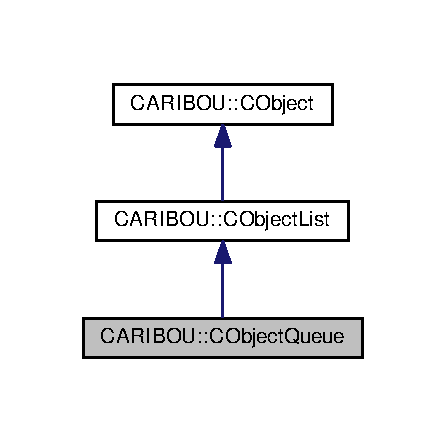
\includegraphics[width=214pt]{class_c_a_r_i_b_o_u_1_1_c_object_queue__inherit__graph}
\end{center}
\end{figure}


Collaboration diagram for C\+A\+R\+I\+B\+OU\+:\+:C\+Object\+Queue\+:
\nopagebreak
\begin{figure}[H]
\begin{center}
\leavevmode
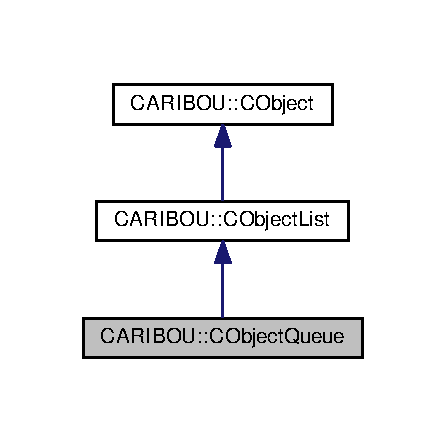
\includegraphics[width=214pt]{class_c_a_r_i_b_o_u_1_1_c_object_queue__coll__graph}
\end{center}
\end{figure}
\subsection*{Public Member Functions}
\begin{DoxyCompactItemize}
\item 
{\bf C\+Object\+Queue} ()
\item 
{\bf $\sim$\+C\+Object\+Queue} ()
\item 
{\bf C\+Object} $\ast$ {\bf dequeue} ()
\begin{DoxyCompactList}\small\item\em Dequeue the object by removing if from list at index [0]. \end{DoxyCompactList}\end{DoxyCompactItemize}
\subsection*{Additional Inherited Members}


\subsection{Detailed Description}
Reimplements a \doxyref{C\+Object\+List}{p.}{class_c_a_r_i_b_o_u_1_1_c_object_list} as a F\+I\+FO queue. 

\begin{DoxyAuthor}{Author}
Michael Sharkey {\tt mike@pikeaero.\+com} 
\end{DoxyAuthor}


Definition at line 30 of file cobjectqueue.\+h.



\subsection{Constructor \& Destructor Documentation}
\index{C\+A\+R\+I\+B\+O\+U\+::\+C\+Object\+Queue@{C\+A\+R\+I\+B\+O\+U\+::\+C\+Object\+Queue}!C\+Object\+Queue@{C\+Object\+Queue}}
\index{C\+Object\+Queue@{C\+Object\+Queue}!C\+A\+R\+I\+B\+O\+U\+::\+C\+Object\+Queue@{C\+A\+R\+I\+B\+O\+U\+::\+C\+Object\+Queue}}
\subsubsection[{C\+Object\+Queue()}]{\setlength{\rightskip}{0pt plus 5cm}C\+A\+R\+I\+B\+O\+U\+::\+C\+Object\+Queue\+::\+C\+Object\+Queue (
\begin{DoxyParamCaption}
{}
\end{DoxyParamCaption}
)}\label{class_c_a_r_i_b_o_u_1_1_c_object_queue_ae4bd444491c4e1a1512d351bbe909f85}


Definition at line 21 of file cobjectqueue.\+cpp.

\index{C\+A\+R\+I\+B\+O\+U\+::\+C\+Object\+Queue@{C\+A\+R\+I\+B\+O\+U\+::\+C\+Object\+Queue}!````~C\+Object\+Queue@{$\sim$\+C\+Object\+Queue}}
\index{````~C\+Object\+Queue@{$\sim$\+C\+Object\+Queue}!C\+A\+R\+I\+B\+O\+U\+::\+C\+Object\+Queue@{C\+A\+R\+I\+B\+O\+U\+::\+C\+Object\+Queue}}
\subsubsection[{$\sim$\+C\+Object\+Queue()}]{\setlength{\rightskip}{0pt plus 5cm}C\+A\+R\+I\+B\+O\+U\+::\+C\+Object\+Queue\+::$\sim$\+C\+Object\+Queue (
\begin{DoxyParamCaption}
{}
\end{DoxyParamCaption}
)}\label{class_c_a_r_i_b_o_u_1_1_c_object_queue_a635851e94341c8456b33724bd5c85f0a}


Definition at line 27 of file cobjectqueue.\+cpp.



\subsection{Member Function Documentation}
\index{C\+A\+R\+I\+B\+O\+U\+::\+C\+Object\+Queue@{C\+A\+R\+I\+B\+O\+U\+::\+C\+Object\+Queue}!dequeue@{dequeue}}
\index{dequeue@{dequeue}!C\+A\+R\+I\+B\+O\+U\+::\+C\+Object\+Queue@{C\+A\+R\+I\+B\+O\+U\+::\+C\+Object\+Queue}}
\subsubsection[{dequeue()}]{\setlength{\rightskip}{0pt plus 5cm}{\bf C\+Object} $\ast$ C\+A\+R\+I\+B\+O\+U\+::\+C\+Object\+Queue\+::dequeue (
\begin{DoxyParamCaption}
{}
\end{DoxyParamCaption}
)}\label{class_c_a_r_i_b_o_u_1_1_c_object_queue_a06d338c492df8de18496be37f6621186}


Dequeue the object by removing if from list at index [0]. 



Definition at line 34 of file cobjectqueue.\+cpp.



The documentation for this class was generated from the following files\+:\begin{DoxyCompactItemize}
\item 
include/caribou++/{\bf cobjectqueue.\+h}\item 
src/{\bf cobjectqueue.\+cpp}\end{DoxyCompactItemize}

\section{C\+A\+R\+I\+B\+OU\+:\+:C\+Pixmap Class Reference}
\label{class_c_a_r_i_b_o_u_1_1_c_pixmap}\index{C\+A\+R\+I\+B\+O\+U\+::\+C\+Pixmap@{C\+A\+R\+I\+B\+O\+U\+::\+C\+Pixmap}}


Defines X\+Pixmap storage class.  




{\ttfamily \#include $<$cpixmap.\+h$>$}



Inheritance diagram for C\+A\+R\+I\+B\+OU\+:\+:C\+Pixmap\+:\nopagebreak
\begin{figure}[H]
\begin{center}
\leavevmode
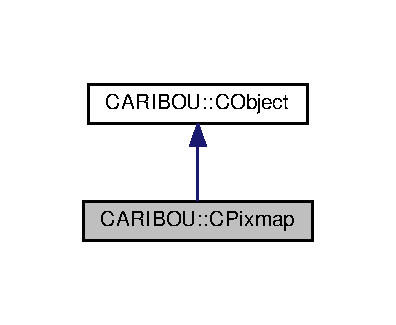
\includegraphics[width=190pt]{class_c_a_r_i_b_o_u_1_1_c_pixmap__inherit__graph}
\end{center}
\end{figure}


Collaboration diagram for C\+A\+R\+I\+B\+OU\+:\+:C\+Pixmap\+:\nopagebreak
\begin{figure}[H]
\begin{center}
\leavevmode
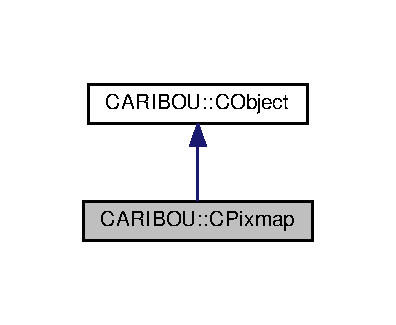
\includegraphics[width=190pt]{class_c_a_r_i_b_o_u_1_1_c_pixmap__coll__graph}
\end{center}
\end{figure}
\subsection*{Public Member Functions}
\begin{DoxyCompactItemize}
\item 
{\bf C\+Pixmap} ()
\item 
{\bf C\+Pixmap} (const char $\ast$data[$\,$])
\item 
{\bf C\+Pixmap} (const {\bf C\+Pixmap} \&other)
\item 
virtual {\bf $\sim$\+C\+Pixmap} ()
\item 
bool {\bf load} (const char $\ast$data[$\,$])
\begin{DoxyCompactList}\small\item\em Load from an in-\/memory X\+PM image. \end{DoxyCompactList}\item 
bool {\bf valid} ()
\item 
void {\bf clear} ()
\item 
int {\bf width} ()
\item 
int {\bf height} ()
\item 
{\bf C\+A\+R\+I\+B\+O\+U\+::\+C\+Size} {\bf size} ()
\item 
{\bf C\+A\+R\+I\+B\+O\+U\+::\+C\+Rect} {\bf bounds} ()
\item 
int {\bf color\+Count} ()
\item 
int {\bf key\+Bytes} ()
\item 
void $\ast$ {\bf pixels} ()
\item 
uint32\+\_\+t $\ast$ {\bf color\+Map} ()
\item 
uint32\+\_\+t {\bf color\+At} (int x, int y)
\item 
uint32\+\_\+t {\bf key\+At} (int x, int y)
\begin{DoxyCompactList}\small\item\em Fetch the color index at the pixel location X,y. \end{DoxyCompactList}\item 
uint32\+\_\+t $\ast$ {\bf colors\+At} (int y)
\begin{DoxyCompactList}\small\item\em Fetch a row of colors into an allocated buffer. \end{DoxyCompactList}\item 
void {\bf set\+Key\+At} (int x, int y, uint32\+\_\+t key)
\begin{DoxyCompactList}\small\item\em Set a pixel color key. \end{DoxyCompactList}\item 
bool {\bf stretch} ({\bf C\+A\+R\+I\+B\+O\+U\+::\+C\+Size} {\bf size})
\begin{DoxyCompactList}\small\item\em Stretch an image about it\textquotesingle{}s horizontal and vertical center-\/lines. \end{DoxyCompactList}\item 
{\bf C\+A\+R\+I\+B\+O\+U\+::\+C\+Size} {\bf get\+Stretch} ()
\end{DoxyCompactItemize}
\subsection*{Additional Inherited Members}


\subsection{Detailed Description}
Defines X\+Pixmap storage class. 



Definition at line 28 of file cpixmap.\+h.



\subsection{Constructor \& Destructor Documentation}
\index{C\+A\+R\+I\+B\+O\+U\+::\+C\+Pixmap@{C\+A\+R\+I\+B\+O\+U\+::\+C\+Pixmap}!C\+Pixmap@{C\+Pixmap}}
\index{C\+Pixmap@{C\+Pixmap}!C\+A\+R\+I\+B\+O\+U\+::\+C\+Pixmap@{C\+A\+R\+I\+B\+O\+U\+::\+C\+Pixmap}}
\subsubsection[{C\+Pixmap()}]{\setlength{\rightskip}{0pt plus 5cm}C\+A\+R\+I\+B\+O\+U\+::\+C\+Pixmap\+::\+C\+Pixmap (
\begin{DoxyParamCaption}
{}
\end{DoxyParamCaption}
)}\label{class_c_a_r_i_b_o_u_1_1_c_pixmap_abb5ea015ed436e07d2e1d786aa1ac8d2}


Definition at line 24 of file cpixmap.\+cpp.

\index{C\+A\+R\+I\+B\+O\+U\+::\+C\+Pixmap@{C\+A\+R\+I\+B\+O\+U\+::\+C\+Pixmap}!C\+Pixmap@{C\+Pixmap}}
\index{C\+Pixmap@{C\+Pixmap}!C\+A\+R\+I\+B\+O\+U\+::\+C\+Pixmap@{C\+A\+R\+I\+B\+O\+U\+::\+C\+Pixmap}}
\subsubsection[{C\+Pixmap(const char $\ast$data[])}]{\setlength{\rightskip}{0pt plus 5cm}C\+A\+R\+I\+B\+O\+U\+::\+C\+Pixmap\+::\+C\+Pixmap (
\begin{DoxyParamCaption}
\item[{const char $\ast$}]{data[$\,$]}
\end{DoxyParamCaption}
)}\label{class_c_a_r_i_b_o_u_1_1_c_pixmap_a395241d58a87c3140d6f07b95423d6d4}


Definition at line 39 of file cpixmap.\+cpp.

\index{C\+A\+R\+I\+B\+O\+U\+::\+C\+Pixmap@{C\+A\+R\+I\+B\+O\+U\+::\+C\+Pixmap}!C\+Pixmap@{C\+Pixmap}}
\index{C\+Pixmap@{C\+Pixmap}!C\+A\+R\+I\+B\+O\+U\+::\+C\+Pixmap@{C\+A\+R\+I\+B\+O\+U\+::\+C\+Pixmap}}
\subsubsection[{C\+Pixmap(const C\+Pixmap \&other)}]{\setlength{\rightskip}{0pt plus 5cm}C\+A\+R\+I\+B\+O\+U\+::\+C\+Pixmap\+::\+C\+Pixmap (
\begin{DoxyParamCaption}
\item[{const {\bf C\+Pixmap} \&}]{other}
\end{DoxyParamCaption}
)}\label{class_c_a_r_i_b_o_u_1_1_c_pixmap_aeffb77f01e41644768b73a3ca908a7ab}


Definition at line 55 of file cpixmap.\+cpp.

\index{C\+A\+R\+I\+B\+O\+U\+::\+C\+Pixmap@{C\+A\+R\+I\+B\+O\+U\+::\+C\+Pixmap}!````~C\+Pixmap@{$\sim$\+C\+Pixmap}}
\index{````~C\+Pixmap@{$\sim$\+C\+Pixmap}!C\+A\+R\+I\+B\+O\+U\+::\+C\+Pixmap@{C\+A\+R\+I\+B\+O\+U\+::\+C\+Pixmap}}
\subsubsection[{$\sim$\+C\+Pixmap()}]{\setlength{\rightskip}{0pt plus 5cm}C\+A\+R\+I\+B\+O\+U\+::\+C\+Pixmap\+::$\sim$\+C\+Pixmap (
\begin{DoxyParamCaption}
{}
\end{DoxyParamCaption}
)\hspace{0.3cm}{\ttfamily [virtual]}}\label{class_c_a_r_i_b_o_u_1_1_c_pixmap_a37bbd283a5642b26f67f4307e6520ad6}


Definition at line 84 of file cpixmap.\+cpp.



\subsection{Member Function Documentation}
\index{C\+A\+R\+I\+B\+O\+U\+::\+C\+Pixmap@{C\+A\+R\+I\+B\+O\+U\+::\+C\+Pixmap}!bounds@{bounds}}
\index{bounds@{bounds}!C\+A\+R\+I\+B\+O\+U\+::\+C\+Pixmap@{C\+A\+R\+I\+B\+O\+U\+::\+C\+Pixmap}}
\subsubsection[{bounds()}]{\setlength{\rightskip}{0pt plus 5cm}{\bf C\+A\+R\+I\+B\+O\+U\+::\+C\+Rect} C\+A\+R\+I\+B\+O\+U\+::\+C\+Pixmap\+::bounds (
\begin{DoxyParamCaption}
{}
\end{DoxyParamCaption}
)\hspace{0.3cm}{\ttfamily [inline]}}\label{class_c_a_r_i_b_o_u_1_1_c_pixmap_a8db7d4b8138428f48197dbb453465618}


Definition at line 43 of file cpixmap.\+h.

\index{C\+A\+R\+I\+B\+O\+U\+::\+C\+Pixmap@{C\+A\+R\+I\+B\+O\+U\+::\+C\+Pixmap}!clear@{clear}}
\index{clear@{clear}!C\+A\+R\+I\+B\+O\+U\+::\+C\+Pixmap@{C\+A\+R\+I\+B\+O\+U\+::\+C\+Pixmap}}
\subsubsection[{clear()}]{\setlength{\rightskip}{0pt plus 5cm}void C\+A\+R\+I\+B\+O\+U\+::\+C\+Pixmap\+::clear (
\begin{DoxyParamCaption}
{}
\end{DoxyParamCaption}
)}\label{class_c_a_r_i_b_o_u_1_1_c_pixmap_a179dd5ad141c5520c047f23be728aa0b}


Definition at line 89 of file cpixmap.\+cpp.

\index{C\+A\+R\+I\+B\+O\+U\+::\+C\+Pixmap@{C\+A\+R\+I\+B\+O\+U\+::\+C\+Pixmap}!color\+At@{color\+At}}
\index{color\+At@{color\+At}!C\+A\+R\+I\+B\+O\+U\+::\+C\+Pixmap@{C\+A\+R\+I\+B\+O\+U\+::\+C\+Pixmap}}
\subsubsection[{color\+At(int x, int y)}]{\setlength{\rightskip}{0pt plus 5cm}uint32\+\_\+t C\+A\+R\+I\+B\+O\+U\+::\+C\+Pixmap\+::color\+At (
\begin{DoxyParamCaption}
\item[{int}]{x, }
\item[{int}]{y}
\end{DoxyParamCaption}
)\hspace{0.3cm}{\ttfamily [inline]}}\label{class_c_a_r_i_b_o_u_1_1_c_pixmap_a5df51acbe11084fc2a33b2f5482e14ce}


Definition at line 48 of file cpixmap.\+h.

\index{C\+A\+R\+I\+B\+O\+U\+::\+C\+Pixmap@{C\+A\+R\+I\+B\+O\+U\+::\+C\+Pixmap}!color\+Count@{color\+Count}}
\index{color\+Count@{color\+Count}!C\+A\+R\+I\+B\+O\+U\+::\+C\+Pixmap@{C\+A\+R\+I\+B\+O\+U\+::\+C\+Pixmap}}
\subsubsection[{color\+Count()}]{\setlength{\rightskip}{0pt plus 5cm}int C\+A\+R\+I\+B\+O\+U\+::\+C\+Pixmap\+::color\+Count (
\begin{DoxyParamCaption}
{}
\end{DoxyParamCaption}
)\hspace{0.3cm}{\ttfamily [inline]}}\label{class_c_a_r_i_b_o_u_1_1_c_pixmap_af5877a0e00a54910dfe1231307b7cf07}


Definition at line 44 of file cpixmap.\+h.

\index{C\+A\+R\+I\+B\+O\+U\+::\+C\+Pixmap@{C\+A\+R\+I\+B\+O\+U\+::\+C\+Pixmap}!color\+Map@{color\+Map}}
\index{color\+Map@{color\+Map}!C\+A\+R\+I\+B\+O\+U\+::\+C\+Pixmap@{C\+A\+R\+I\+B\+O\+U\+::\+C\+Pixmap}}
\subsubsection[{color\+Map()}]{\setlength{\rightskip}{0pt plus 5cm}uint32\+\_\+t$\ast$ C\+A\+R\+I\+B\+O\+U\+::\+C\+Pixmap\+::color\+Map (
\begin{DoxyParamCaption}
{}
\end{DoxyParamCaption}
)\hspace{0.3cm}{\ttfamily [inline]}}\label{class_c_a_r_i_b_o_u_1_1_c_pixmap_aeaf796c7f9b74cc51e6d61d345d8854a}


Definition at line 47 of file cpixmap.\+h.

\index{C\+A\+R\+I\+B\+O\+U\+::\+C\+Pixmap@{C\+A\+R\+I\+B\+O\+U\+::\+C\+Pixmap}!colors\+At@{colors\+At}}
\index{colors\+At@{colors\+At}!C\+A\+R\+I\+B\+O\+U\+::\+C\+Pixmap@{C\+A\+R\+I\+B\+O\+U\+::\+C\+Pixmap}}
\subsubsection[{colors\+At(int y)}]{\setlength{\rightskip}{0pt plus 5cm}uint32\+\_\+t $\ast$ C\+A\+R\+I\+B\+O\+U\+::\+C\+Pixmap\+::colors\+At (
\begin{DoxyParamCaption}
\item[{int}]{y}
\end{DoxyParamCaption}
)}\label{class_c_a_r_i_b_o_u_1_1_c_pixmap_a3ea16a6e0c546c736d97a82c3d87c205}


Fetch a row of colors into an allocated buffer. 

\begin{DoxyReturn}{Returns}
a pointer to a buffer of R\+GB values \doxyref{width()}{p.}{class_c_a_r_i_b_o_u_1_1_c_pixmap_ac2aaadc7bf00dc8eff1c8465b7571ca8} words long. 
\end{DoxyReturn}


Definition at line 205 of file cpixmap.\+cpp.

\index{C\+A\+R\+I\+B\+O\+U\+::\+C\+Pixmap@{C\+A\+R\+I\+B\+O\+U\+::\+C\+Pixmap}!get\+Stretch@{get\+Stretch}}
\index{get\+Stretch@{get\+Stretch}!C\+A\+R\+I\+B\+O\+U\+::\+C\+Pixmap@{C\+A\+R\+I\+B\+O\+U\+::\+C\+Pixmap}}
\subsubsection[{get\+Stretch()}]{\setlength{\rightskip}{0pt plus 5cm}{\bf C\+A\+R\+I\+B\+O\+U\+::\+C\+Size} C\+A\+R\+I\+B\+O\+U\+::\+C\+Pixmap\+::get\+Stretch (
\begin{DoxyParamCaption}
{}
\end{DoxyParamCaption}
)\hspace{0.3cm}{\ttfamily [inline]}}\label{class_c_a_r_i_b_o_u_1_1_c_pixmap_a06adf6a512744828d12ae212a8de4fa9}


Definition at line 53 of file cpixmap.\+h.

\index{C\+A\+R\+I\+B\+O\+U\+::\+C\+Pixmap@{C\+A\+R\+I\+B\+O\+U\+::\+C\+Pixmap}!height@{height}}
\index{height@{height}!C\+A\+R\+I\+B\+O\+U\+::\+C\+Pixmap@{C\+A\+R\+I\+B\+O\+U\+::\+C\+Pixmap}}
\subsubsection[{height()}]{\setlength{\rightskip}{0pt plus 5cm}int C\+A\+R\+I\+B\+O\+U\+::\+C\+Pixmap\+::height (
\begin{DoxyParamCaption}
{}
\end{DoxyParamCaption}
)\hspace{0.3cm}{\ttfamily [inline]}}\label{class_c_a_r_i_b_o_u_1_1_c_pixmap_a0a4ea802b143837d4c33c49b0f98973e}


Definition at line 41 of file cpixmap.\+h.

\index{C\+A\+R\+I\+B\+O\+U\+::\+C\+Pixmap@{C\+A\+R\+I\+B\+O\+U\+::\+C\+Pixmap}!key\+At@{key\+At}}
\index{key\+At@{key\+At}!C\+A\+R\+I\+B\+O\+U\+::\+C\+Pixmap@{C\+A\+R\+I\+B\+O\+U\+::\+C\+Pixmap}}
\subsubsection[{key\+At(int x, int y)}]{\setlength{\rightskip}{0pt plus 5cm}uint32\+\_\+t C\+A\+R\+I\+B\+O\+U\+::\+C\+Pixmap\+::key\+At (
\begin{DoxyParamCaption}
\item[{int}]{x, }
\item[{int}]{y}
\end{DoxyParamCaption}
)}\label{class_c_a_r_i_b_o_u_1_1_c_pixmap_a41b28cdc10cf19a51c8994a746ef695b}


Fetch the color index at the pixel location X,y. 



Definition at line 232 of file cpixmap.\+cpp.

\index{C\+A\+R\+I\+B\+O\+U\+::\+C\+Pixmap@{C\+A\+R\+I\+B\+O\+U\+::\+C\+Pixmap}!key\+Bytes@{key\+Bytes}}
\index{key\+Bytes@{key\+Bytes}!C\+A\+R\+I\+B\+O\+U\+::\+C\+Pixmap@{C\+A\+R\+I\+B\+O\+U\+::\+C\+Pixmap}}
\subsubsection[{key\+Bytes()}]{\setlength{\rightskip}{0pt plus 5cm}int C\+A\+R\+I\+B\+O\+U\+::\+C\+Pixmap\+::key\+Bytes (
\begin{DoxyParamCaption}
{}
\end{DoxyParamCaption}
)\hspace{0.3cm}{\ttfamily [inline]}}\label{class_c_a_r_i_b_o_u_1_1_c_pixmap_aaddc340979cc24b91d28175b3c57f1ab}


Definition at line 45 of file cpixmap.\+h.

\index{C\+A\+R\+I\+B\+O\+U\+::\+C\+Pixmap@{C\+A\+R\+I\+B\+O\+U\+::\+C\+Pixmap}!load@{load}}
\index{load@{load}!C\+A\+R\+I\+B\+O\+U\+::\+C\+Pixmap@{C\+A\+R\+I\+B\+O\+U\+::\+C\+Pixmap}}
\subsubsection[{load(const char $\ast$data[])}]{\setlength{\rightskip}{0pt plus 5cm}bool C\+A\+R\+I\+B\+O\+U\+::\+C\+Pixmap\+::load (
\begin{DoxyParamCaption}
\item[{const char $\ast$}]{data[$\,$]}
\end{DoxyParamCaption}
)}\label{class_c_a_r_i_b_o_u_1_1_c_pixmap_a2a7e647afdf6aa74033100cebe5b93f7}


Load from an in-\/memory X\+PM image. 

Re-\/map the color table for faster lookup. 

Definition at line 326 of file cpixmap.\+cpp.

\index{C\+A\+R\+I\+B\+O\+U\+::\+C\+Pixmap@{C\+A\+R\+I\+B\+O\+U\+::\+C\+Pixmap}!pixels@{pixels}}
\index{pixels@{pixels}!C\+A\+R\+I\+B\+O\+U\+::\+C\+Pixmap@{C\+A\+R\+I\+B\+O\+U\+::\+C\+Pixmap}}
\subsubsection[{pixels()}]{\setlength{\rightskip}{0pt plus 5cm}void$\ast$ C\+A\+R\+I\+B\+O\+U\+::\+C\+Pixmap\+::pixels (
\begin{DoxyParamCaption}
{}
\end{DoxyParamCaption}
)\hspace{0.3cm}{\ttfamily [inline]}}\label{class_c_a_r_i_b_o_u_1_1_c_pixmap_a3a3a27a175e7ef467b5793d46ecd3ccd}


Definition at line 46 of file cpixmap.\+h.

\index{C\+A\+R\+I\+B\+O\+U\+::\+C\+Pixmap@{C\+A\+R\+I\+B\+O\+U\+::\+C\+Pixmap}!set\+Key\+At@{set\+Key\+At}}
\index{set\+Key\+At@{set\+Key\+At}!C\+A\+R\+I\+B\+O\+U\+::\+C\+Pixmap@{C\+A\+R\+I\+B\+O\+U\+::\+C\+Pixmap}}
\subsubsection[{set\+Key\+At(int x, int y, uint32\+\_\+t key)}]{\setlength{\rightskip}{0pt plus 5cm}void C\+A\+R\+I\+B\+O\+U\+::\+C\+Pixmap\+::set\+Key\+At (
\begin{DoxyParamCaption}
\item[{int}]{x, }
\item[{int}]{y, }
\item[{uint32\+\_\+t}]{key}
\end{DoxyParamCaption}
)}\label{class_c_a_r_i_b_o_u_1_1_c_pixmap_aea64db8faa92fb9b8cfc8962407265a9}


Set a pixel color key. 



Definition at line 352 of file cpixmap.\+cpp.

\index{C\+A\+R\+I\+B\+O\+U\+::\+C\+Pixmap@{C\+A\+R\+I\+B\+O\+U\+::\+C\+Pixmap}!size@{size}}
\index{size@{size}!C\+A\+R\+I\+B\+O\+U\+::\+C\+Pixmap@{C\+A\+R\+I\+B\+O\+U\+::\+C\+Pixmap}}
\subsubsection[{size()}]{\setlength{\rightskip}{0pt plus 5cm}{\bf C\+A\+R\+I\+B\+O\+U\+::\+C\+Size} C\+A\+R\+I\+B\+O\+U\+::\+C\+Pixmap\+::size (
\begin{DoxyParamCaption}
{}
\end{DoxyParamCaption}
)\hspace{0.3cm}{\ttfamily [inline]}}\label{class_c_a_r_i_b_o_u_1_1_c_pixmap_a89994606e83dbdeb9e536541f162ff1c}


Definition at line 42 of file cpixmap.\+h.

\index{C\+A\+R\+I\+B\+O\+U\+::\+C\+Pixmap@{C\+A\+R\+I\+B\+O\+U\+::\+C\+Pixmap}!stretch@{stretch}}
\index{stretch@{stretch}!C\+A\+R\+I\+B\+O\+U\+::\+C\+Pixmap@{C\+A\+R\+I\+B\+O\+U\+::\+C\+Pixmap}}
\subsubsection[{stretch(\+C\+A\+R\+I\+B\+O\+U\+::\+C\+Size size)}]{\setlength{\rightskip}{0pt plus 5cm}bool C\+A\+R\+I\+B\+O\+U\+::\+C\+Pixmap\+::stretch (
\begin{DoxyParamCaption}
\item[{{\bf C\+A\+R\+I\+B\+O\+U\+::\+C\+Size}}]{size}
\end{DoxyParamCaption}
)}\label{class_c_a_r_i_b_o_u_1_1_c_pixmap_ac8403c6333c8756660068726c0f0abed}


Stretch an image about it\textquotesingle{}s horizontal and vertical center-\/lines. 



Definition at line 476 of file cpixmap.\+cpp.

\index{C\+A\+R\+I\+B\+O\+U\+::\+C\+Pixmap@{C\+A\+R\+I\+B\+O\+U\+::\+C\+Pixmap}!valid@{valid}}
\index{valid@{valid}!C\+A\+R\+I\+B\+O\+U\+::\+C\+Pixmap@{C\+A\+R\+I\+B\+O\+U\+::\+C\+Pixmap}}
\subsubsection[{valid()}]{\setlength{\rightskip}{0pt plus 5cm}bool C\+A\+R\+I\+B\+O\+U\+::\+C\+Pixmap\+::valid (
\begin{DoxyParamCaption}
{}
\end{DoxyParamCaption}
)\hspace{0.3cm}{\ttfamily [inline]}}\label{class_c_a_r_i_b_o_u_1_1_c_pixmap_a30bd68ebf1bd953f9b4f1eeb281207ec}


Definition at line 37 of file cpixmap.\+h.

\index{C\+A\+R\+I\+B\+O\+U\+::\+C\+Pixmap@{C\+A\+R\+I\+B\+O\+U\+::\+C\+Pixmap}!width@{width}}
\index{width@{width}!C\+A\+R\+I\+B\+O\+U\+::\+C\+Pixmap@{C\+A\+R\+I\+B\+O\+U\+::\+C\+Pixmap}}
\subsubsection[{width()}]{\setlength{\rightskip}{0pt plus 5cm}int C\+A\+R\+I\+B\+O\+U\+::\+C\+Pixmap\+::width (
\begin{DoxyParamCaption}
{}
\end{DoxyParamCaption}
)\hspace{0.3cm}{\ttfamily [inline]}}\label{class_c_a_r_i_b_o_u_1_1_c_pixmap_ac2aaadc7bf00dc8eff1c8465b7571ca8}


Definition at line 40 of file cpixmap.\+h.



The documentation for this class was generated from the following files\+:\begin{DoxyCompactItemize}
\item 
include/caribou++/{\bf cpixmap.\+h}\item 
src/{\bf cpixmap.\+cpp}\end{DoxyCompactItemize}

\section{C\-A\-R\-I\-B\-O\-U\-:\-:C\-Point Class Reference}
\label{class_c_a_r_i_b_o_u_1_1_c_point}\index{C\-A\-R\-I\-B\-O\-U\-::\-C\-Point@{C\-A\-R\-I\-B\-O\-U\-::\-C\-Point}}


{\ttfamily \#include $<$cpoint.\-h$>$}

\subsection*{Public Member Functions}
\begin{DoxyCompactItemize}
\item 
{\bf C\-Point} ()
\item 
{\bf C\-Point} (int16\-\_\-t {\bf x}, int16\-\_\-t {\bf y})
\item 
{\bf C\-Point} (const {\bf C\-Point} \&other)
\item 
{\bf $\sim$\-C\-Point} ()
\item 
void {\bf copy} (const {\bf C\-Point} \&other)
\item 
void {\bf set\-X\-Y} (int16\-\_\-t {\bf x}, int16\-\_\-t {\bf y})
\item 
void {\bf set\-X} (int16\-\_\-t {\bf x})
\item 
void {\bf set\-Y} (int16\-\_\-t {\bf y})
\item 
int16\-\_\-t {\bf x} ()
\item 
int16\-\_\-t {\bf y} ()
\item 
{\bf C\-Point} \& {\bf add} (const {\bf C\-Point} \&other)
\begin{DoxyCompactList}\small\item\em Add an offset from another point. \end{DoxyCompactList}\item 
{\bf C\-Point} \& {\bf subtract} (const {\bf C\-Point} \&other)
\begin{DoxyCompactList}\small\item\em Subtract an offset from another point. \end{DoxyCompactList}\item 
{\bf C\-Point} \& {\bf operator=} (const {\bf C\-Point} \&other)
\item 
{\bf C\-Point} \& {\bf operator+=} (const {\bf C\-Point} \&other)
\item 
{\bf C\-Point} \& {\bf operator-\/=} (const {\bf C\-Point} \&other)
\item 
bool {\bf operator==} (const {\bf C\-Point} \&other)
\item 
bool {\bf operator!=} (const {\bf C\-Point} \&other)
\end{DoxyCompactItemize}


\subsection{Detailed Description}


Definition at line 25 of file cpoint.\-h.



\subsection{Constructor \& Destructor Documentation}
\index{C\-A\-R\-I\-B\-O\-U\-::\-C\-Point@{C\-A\-R\-I\-B\-O\-U\-::\-C\-Point}!C\-Point@{C\-Point}}
\index{C\-Point@{C\-Point}!CARIBOU::CPoint@{C\-A\-R\-I\-B\-O\-U\-::\-C\-Point}}
\subsubsection[{C\-Point}]{\setlength{\rightskip}{0pt plus 5cm}C\-A\-R\-I\-B\-O\-U\-::\-C\-Point\-::\-C\-Point (
\begin{DoxyParamCaption}
{}
\end{DoxyParamCaption}
)}\label{class_c_a_r_i_b_o_u_1_1_c_point_a58d1a30895ccd63d8605c5b266956902}


Definition at line 21 of file cpoint.\-cpp.

\index{C\-A\-R\-I\-B\-O\-U\-::\-C\-Point@{C\-A\-R\-I\-B\-O\-U\-::\-C\-Point}!C\-Point@{C\-Point}}
\index{C\-Point@{C\-Point}!CARIBOU::CPoint@{C\-A\-R\-I\-B\-O\-U\-::\-C\-Point}}
\subsubsection[{C\-Point}]{\setlength{\rightskip}{0pt plus 5cm}C\-A\-R\-I\-B\-O\-U\-::\-C\-Point\-::\-C\-Point (
\begin{DoxyParamCaption}
\item[{int16\-\_\-t}]{x, }
\item[{int16\-\_\-t}]{y}
\end{DoxyParamCaption}
)}\label{class_c_a_r_i_b_o_u_1_1_c_point_a7a4cae3514b6f48547bedd0da3a004fb}


Definition at line 27 of file cpoint.\-cpp.

\index{C\-A\-R\-I\-B\-O\-U\-::\-C\-Point@{C\-A\-R\-I\-B\-O\-U\-::\-C\-Point}!C\-Point@{C\-Point}}
\index{C\-Point@{C\-Point}!CARIBOU::CPoint@{C\-A\-R\-I\-B\-O\-U\-::\-C\-Point}}
\subsubsection[{C\-Point}]{\setlength{\rightskip}{0pt plus 5cm}C\-A\-R\-I\-B\-O\-U\-::\-C\-Point\-::\-C\-Point (
\begin{DoxyParamCaption}
\item[{const {\bf C\-Point} \&}]{other}
\end{DoxyParamCaption}
)}\label{class_c_a_r_i_b_o_u_1_1_c_point_ad8469df974fea47c9e87c37c98fc645d}


Definition at line 33 of file cpoint.\-cpp.

\index{C\-A\-R\-I\-B\-O\-U\-::\-C\-Point@{C\-A\-R\-I\-B\-O\-U\-::\-C\-Point}!$\sim$\-C\-Point@{$\sim$\-C\-Point}}
\index{$\sim$\-C\-Point@{$\sim$\-C\-Point}!CARIBOU::CPoint@{C\-A\-R\-I\-B\-O\-U\-::\-C\-Point}}
\subsubsection[{$\sim$\-C\-Point}]{\setlength{\rightskip}{0pt plus 5cm}C\-A\-R\-I\-B\-O\-U\-::\-C\-Point\-::$\sim$\-C\-Point (
\begin{DoxyParamCaption}
{}
\end{DoxyParamCaption}
)}\label{class_c_a_r_i_b_o_u_1_1_c_point_aae348154d35800e8859411d356365158}


Definition at line 39 of file cpoint.\-cpp.



\subsection{Member Function Documentation}
\index{C\-A\-R\-I\-B\-O\-U\-::\-C\-Point@{C\-A\-R\-I\-B\-O\-U\-::\-C\-Point}!add@{add}}
\index{add@{add}!CARIBOU::CPoint@{C\-A\-R\-I\-B\-O\-U\-::\-C\-Point}}
\subsubsection[{add}]{\setlength{\rightskip}{0pt plus 5cm}{\bf C\-Point} \& C\-A\-R\-I\-B\-O\-U\-::\-C\-Point\-::add (
\begin{DoxyParamCaption}
\item[{const {\bf C\-Point} \&}]{other}
\end{DoxyParamCaption}
)}\label{class_c_a_r_i_b_o_u_1_1_c_point_a7eceebe9c74439ac13d3db4261cb1a79}


Add an offset from another point. 



Definition at line 46 of file cpoint.\-cpp.

\index{C\-A\-R\-I\-B\-O\-U\-::\-C\-Point@{C\-A\-R\-I\-B\-O\-U\-::\-C\-Point}!copy@{copy}}
\index{copy@{copy}!CARIBOU::CPoint@{C\-A\-R\-I\-B\-O\-U\-::\-C\-Point}}
\subsubsection[{copy}]{\setlength{\rightskip}{0pt plus 5cm}void C\-A\-R\-I\-B\-O\-U\-::\-C\-Point\-::copy (
\begin{DoxyParamCaption}
\item[{const {\bf C\-Point} \&}]{other}
\end{DoxyParamCaption}
)\hspace{0.3cm}{\ttfamily [inline]}}\label{class_c_a_r_i_b_o_u_1_1_c_point_ae16145a4df007e9ce6c07d74bfd1d4fa}


Definition at line 33 of file cpoint.\-h.

\index{C\-A\-R\-I\-B\-O\-U\-::\-C\-Point@{C\-A\-R\-I\-B\-O\-U\-::\-C\-Point}!operator!=@{operator!=}}
\index{operator!=@{operator!=}!CARIBOU::CPoint@{C\-A\-R\-I\-B\-O\-U\-::\-C\-Point}}
\subsubsection[{operator!=}]{\setlength{\rightskip}{0pt plus 5cm}bool C\-A\-R\-I\-B\-O\-U\-::\-C\-Point\-::operator!= (
\begin{DoxyParamCaption}
\item[{const {\bf C\-Point} \&}]{other}
\end{DoxyParamCaption}
)}\label{class_c_a_r_i_b_o_u_1_1_c_point_a93cf102c1ed448c92fd296496053e335}


Definition at line 75 of file cpoint.\-cpp.

\index{C\-A\-R\-I\-B\-O\-U\-::\-C\-Point@{C\-A\-R\-I\-B\-O\-U\-::\-C\-Point}!operator+=@{operator+=}}
\index{operator+=@{operator+=}!CARIBOU::CPoint@{C\-A\-R\-I\-B\-O\-U\-::\-C\-Point}}
\subsubsection[{operator+=}]{\setlength{\rightskip}{0pt plus 5cm}{\bf C\-Point}\& C\-A\-R\-I\-B\-O\-U\-::\-C\-Point\-::operator+= (
\begin{DoxyParamCaption}
\item[{const {\bf C\-Point} \&}]{other}
\end{DoxyParamCaption}
)\hspace{0.3cm}{\ttfamily [inline]}}\label{class_c_a_r_i_b_o_u_1_1_c_point_a1312b61743e7c2a19104367c3fd2ca30}


Definition at line 46 of file cpoint.\-h.

\index{C\-A\-R\-I\-B\-O\-U\-::\-C\-Point@{C\-A\-R\-I\-B\-O\-U\-::\-C\-Point}!operator-\/=@{operator-\/=}}
\index{operator-\/=@{operator-\/=}!CARIBOU::CPoint@{C\-A\-R\-I\-B\-O\-U\-::\-C\-Point}}
\subsubsection[{operator-\/=}]{\setlength{\rightskip}{0pt plus 5cm}{\bf C\-Point}\& C\-A\-R\-I\-B\-O\-U\-::\-C\-Point\-::operator-\/= (
\begin{DoxyParamCaption}
\item[{const {\bf C\-Point} \&}]{other}
\end{DoxyParamCaption}
)\hspace{0.3cm}{\ttfamily [inline]}}\label{class_c_a_r_i_b_o_u_1_1_c_point_aa0dfac536a3d2d5eebc440037d9bdff3}


Definition at line 53 of file cpoint.\-h.

\index{C\-A\-R\-I\-B\-O\-U\-::\-C\-Point@{C\-A\-R\-I\-B\-O\-U\-::\-C\-Point}!operator=@{operator=}}
\index{operator=@{operator=}!CARIBOU::CPoint@{C\-A\-R\-I\-B\-O\-U\-::\-C\-Point}}
\subsubsection[{operator=}]{\setlength{\rightskip}{0pt plus 5cm}{\bf C\-Point} \& C\-A\-R\-I\-B\-O\-U\-::\-C\-Point\-::operator= (
\begin{DoxyParamCaption}
\item[{const {\bf C\-Point} \&}]{other}
\end{DoxyParamCaption}
)}\label{class_c_a_r_i_b_o_u_1_1_c_point_ad665a97efea024dd1b4a3e5c5e2af27e}


Definition at line 63 of file cpoint.\-cpp.

\index{C\-A\-R\-I\-B\-O\-U\-::\-C\-Point@{C\-A\-R\-I\-B\-O\-U\-::\-C\-Point}!operator==@{operator==}}
\index{operator==@{operator==}!CARIBOU::CPoint@{C\-A\-R\-I\-B\-O\-U\-::\-C\-Point}}
\subsubsection[{operator==}]{\setlength{\rightskip}{0pt plus 5cm}bool C\-A\-R\-I\-B\-O\-U\-::\-C\-Point\-::operator== (
\begin{DoxyParamCaption}
\item[{const {\bf C\-Point} \&}]{other}
\end{DoxyParamCaption}
)}\label{class_c_a_r_i_b_o_u_1_1_c_point_a472ab78d9f4d833f3f6e9cbc580284de}


Definition at line 70 of file cpoint.\-cpp.

\index{C\-A\-R\-I\-B\-O\-U\-::\-C\-Point@{C\-A\-R\-I\-B\-O\-U\-::\-C\-Point}!set\-X@{set\-X}}
\index{set\-X@{set\-X}!CARIBOU::CPoint@{C\-A\-R\-I\-B\-O\-U\-::\-C\-Point}}
\subsubsection[{set\-X}]{\setlength{\rightskip}{0pt plus 5cm}void C\-A\-R\-I\-B\-O\-U\-::\-C\-Point\-::set\-X (
\begin{DoxyParamCaption}
\item[{int16\-\_\-t}]{x}
\end{DoxyParamCaption}
)\hspace{0.3cm}{\ttfamily [inline]}}\label{class_c_a_r_i_b_o_u_1_1_c_point_a6012fb3c70d5033c459a590e4a1fc080}


Definition at line 35 of file cpoint.\-h.

\index{C\-A\-R\-I\-B\-O\-U\-::\-C\-Point@{C\-A\-R\-I\-B\-O\-U\-::\-C\-Point}!set\-X\-Y@{set\-X\-Y}}
\index{set\-X\-Y@{set\-X\-Y}!CARIBOU::CPoint@{C\-A\-R\-I\-B\-O\-U\-::\-C\-Point}}
\subsubsection[{set\-X\-Y}]{\setlength{\rightskip}{0pt plus 5cm}void C\-A\-R\-I\-B\-O\-U\-::\-C\-Point\-::set\-X\-Y (
\begin{DoxyParamCaption}
\item[{int16\-\_\-t}]{x, }
\item[{int16\-\_\-t}]{y}
\end{DoxyParamCaption}
)\hspace{0.3cm}{\ttfamily [inline]}}\label{class_c_a_r_i_b_o_u_1_1_c_point_a7c65ccdb3fa8e397da455ff7f99c71ee}


Definition at line 34 of file cpoint.\-h.

\index{C\-A\-R\-I\-B\-O\-U\-::\-C\-Point@{C\-A\-R\-I\-B\-O\-U\-::\-C\-Point}!set\-Y@{set\-Y}}
\index{set\-Y@{set\-Y}!CARIBOU::CPoint@{C\-A\-R\-I\-B\-O\-U\-::\-C\-Point}}
\subsubsection[{set\-Y}]{\setlength{\rightskip}{0pt plus 5cm}void C\-A\-R\-I\-B\-O\-U\-::\-C\-Point\-::set\-Y (
\begin{DoxyParamCaption}
\item[{int16\-\_\-t}]{y}
\end{DoxyParamCaption}
)\hspace{0.3cm}{\ttfamily [inline]}}\label{class_c_a_r_i_b_o_u_1_1_c_point_ac7b5947e12261cea9def668e16c27872}


Definition at line 36 of file cpoint.\-h.

\index{C\-A\-R\-I\-B\-O\-U\-::\-C\-Point@{C\-A\-R\-I\-B\-O\-U\-::\-C\-Point}!subtract@{subtract}}
\index{subtract@{subtract}!CARIBOU::CPoint@{C\-A\-R\-I\-B\-O\-U\-::\-C\-Point}}
\subsubsection[{subtract}]{\setlength{\rightskip}{0pt plus 5cm}{\bf C\-Point} \& C\-A\-R\-I\-B\-O\-U\-::\-C\-Point\-::subtract (
\begin{DoxyParamCaption}
\item[{const {\bf C\-Point} \&}]{other}
\end{DoxyParamCaption}
)}\label{class_c_a_r_i_b_o_u_1_1_c_point_a791465241e4cc52df9f4c4b61807680c}


Subtract an offset from another point. 



Definition at line 56 of file cpoint.\-cpp.

\index{C\-A\-R\-I\-B\-O\-U\-::\-C\-Point@{C\-A\-R\-I\-B\-O\-U\-::\-C\-Point}!x@{x}}
\index{x@{x}!CARIBOU::CPoint@{C\-A\-R\-I\-B\-O\-U\-::\-C\-Point}}
\subsubsection[{x}]{\setlength{\rightskip}{0pt plus 5cm}int16\-\_\-t C\-A\-R\-I\-B\-O\-U\-::\-C\-Point\-::x (
\begin{DoxyParamCaption}
{}
\end{DoxyParamCaption}
)\hspace{0.3cm}{\ttfamily [inline]}}\label{class_c_a_r_i_b_o_u_1_1_c_point_a298fa2fe6086d671e77ec6ddc6e570fc}


Definition at line 38 of file cpoint.\-h.

\index{C\-A\-R\-I\-B\-O\-U\-::\-C\-Point@{C\-A\-R\-I\-B\-O\-U\-::\-C\-Point}!y@{y}}
\index{y@{y}!CARIBOU::CPoint@{C\-A\-R\-I\-B\-O\-U\-::\-C\-Point}}
\subsubsection[{y}]{\setlength{\rightskip}{0pt plus 5cm}int16\-\_\-t C\-A\-R\-I\-B\-O\-U\-::\-C\-Point\-::y (
\begin{DoxyParamCaption}
{}
\end{DoxyParamCaption}
)\hspace{0.3cm}{\ttfamily [inline]}}\label{class_c_a_r_i_b_o_u_1_1_c_point_a83e2e9e53eed940754fb79c088d9942a}


Definition at line 39 of file cpoint.\-h.



The documentation for this class was generated from the following files\-:\begin{DoxyCompactItemize}
\item 
include/caribou++/{\bf cpoint.\-h}\item 
src/{\bf cpoint.\-cpp}\end{DoxyCompactItemize}

\section{C\+A\+R\+I\+B\+OU\+:\+:C\+Rect Class Reference}
\label{class_c_a_r_i_b_o_u_1_1_c_rect}\index{C\+A\+R\+I\+B\+O\+U\+::\+C\+Rect@{C\+A\+R\+I\+B\+O\+U\+::\+C\+Rect}}


{\ttfamily \#include $<$crect.\+h$>$}



Inheritance diagram for C\+A\+R\+I\+B\+OU\+:\+:C\+Rect\+:\nopagebreak
\begin{figure}[H]
\begin{center}
\leavevmode
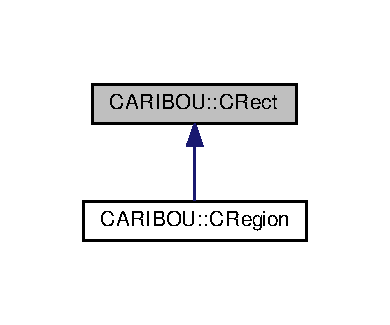
\includegraphics[width=187pt]{class_c_a_r_i_b_o_u_1_1_c_rect__inherit__graph}
\end{center}
\end{figure}
\subsection*{Public Member Functions}
\begin{DoxyCompactItemize}
\item 
{\bf C\+Rect} ()
\item 
{\bf C\+Rect} (int16\+\_\+t {\bf x}, int16\+\_\+t {\bf y}, int16\+\_\+t {\bf width}, int16\+\_\+t {\bf height})
\item 
{\bf C\+Rect} ({\bf C\+Point} {\bf pos}, {\bf C\+Size} {\bf size})
\item 
{\bf C\+Rect} (const {\bf C\+Rect} \&other)
\item 
{\bf $\sim$\+C\+Rect} ()
\item 
{\bf C\+Point} \& {\bf top\+Left} ()
\item 
{\bf C\+Point} {\bf top\+Right} ()
\item 
{\bf C\+Point} {\bf bottom\+Right} ()
\item 
{\bf C\+Point} {\bf bottom\+Left} ()
\item 
void {\bf move} (int16\+\_\+t {\bf x}, int16\+\_\+t {\bf y})
\item 
void {\bf move} ({\bf C\+Point} pt)
\item 
void {\bf set\+Pos} (int16\+\_\+t {\bf x}, int16\+\_\+t {\bf y})
\item 
void {\bf set\+Pos} ({\bf C\+Point} {\bf pos})
\item 
void {\bf resize} (int16\+\_\+t w, int16\+\_\+t h)
\item 
void {\bf resize} ({\bf C\+Size} {\bf size})
\item 
void {\bf setY} (int16\+\_\+t {\bf y})
\item 
void {\bf setX} (int16\+\_\+t {\bf x})
\item 
void {\bf set\+Top} (int16\+\_\+t {\bf top})
\item 
void {\bf set\+Left} (int16\+\_\+t {\bf left})
\item 
void {\bf set\+Bottom} (int16\+\_\+t {\bf bottom})
\item 
void {\bf set\+Right} (int16\+\_\+t {\bf right})
\item 
void {\bf set\+Height} (int16\+\_\+t {\bf height})
\item 
void {\bf set\+Width} (int16\+\_\+t {\bf width})
\item 
void {\bf set\+Size} ({\bf C\+Size} {\bf size})
\item 
{\bf C\+Point} \& {\bf pos} ()
\item 
{\bf C\+Size} \& {\bf size} ()
\item 
int16\+\_\+t {\bf x} ()
\item 
int16\+\_\+t {\bf y} ()
\item 
int16\+\_\+t {\bf width} ()
\item 
int16\+\_\+t {\bf height} ()
\item 
int16\+\_\+t {\bf top} ()
\item 
int16\+\_\+t {\bf left} ()
\item 
int16\+\_\+t {\bf right} ()
\item 
int16\+\_\+t {\bf bottom} ()
\item 
bool {\bf is\+Empty} ()
\item 
{\bf C\+Rect} {\bf inset} (int {\bf x}, int {\bf y}, int w, int h)
\item 
{\bf C\+Rect} \& {\bf operator=} (const {\bf C\+Rect} \&other)
\item 
bool {\bf operator==} (const {\bf C\+Rect} \&other)
\item 
bool {\bf operator!=} (const {\bf C\+Rect} \&other)
\item 
bool {\bf contains} ({\bf C\+Point} \&pt)
\begin{DoxyCompactList}\small\item\em Returns true if the point (x, y) is inside of the rectangle,. \end{DoxyCompactList}\item 
bool {\bf contains} ({\bf C\+Rect} \&rect, bool proper=false)
\begin{DoxyCompactList}\small\item\em Return true if rect is inside of this rectangle (fully inside if proper). \end{DoxyCompactList}\item 
bool {\bf intersects} ({\bf C\+Rect} \&rect)
\item 
{\bf C\+Rect} {\bf intersected} ({\bf C\+Rect} \&rect)
\begin{DoxyCompactList}\small\item\em Returns the intersection of this rectangle and the given rectangle. \end{DoxyCompactList}\item 
{\bf C\+Rect} {\bf united} ({\bf C\+Rect} \&rect)
\begin{DoxyCompactList}\small\item\em Returns the bounding rectangle of this rectangle and the given rectangle. \end{DoxyCompactList}\item 
{\bf C\+Point} {\bf center} ()
\end{DoxyCompactItemize}
\subsection*{Static Public Member Functions}
\begin{DoxyCompactItemize}
\item 
static {\bf C\+Rect} {\bf triangle\+Rect} ({\bf C\+A\+R\+I\+B\+O\+U\+::\+C\+Point} p0, {\bf C\+A\+R\+I\+B\+O\+U\+::\+C\+Point} p1, {\bf C\+A\+R\+I\+B\+O\+U\+::\+C\+Point} p2)
\end{DoxyCompactItemize}


\subsection{Detailed Description}


Definition at line 26 of file crect.\+h.



\subsection{Constructor \& Destructor Documentation}
\index{C\+A\+R\+I\+B\+O\+U\+::\+C\+Rect@{C\+A\+R\+I\+B\+O\+U\+::\+C\+Rect}!C\+Rect@{C\+Rect}}
\index{C\+Rect@{C\+Rect}!C\+A\+R\+I\+B\+O\+U\+::\+C\+Rect@{C\+A\+R\+I\+B\+O\+U\+::\+C\+Rect}}
\subsubsection[{C\+Rect()}]{\setlength{\rightskip}{0pt plus 5cm}C\+A\+R\+I\+B\+O\+U\+::\+C\+Rect\+::\+C\+Rect (
\begin{DoxyParamCaption}
{}
\end{DoxyParamCaption}
)}\label{class_c_a_r_i_b_o_u_1_1_c_rect_a2ffe5187806a5370f8b73f89f76a5809}


Definition at line 21 of file crect.\+cpp.

\index{C\+A\+R\+I\+B\+O\+U\+::\+C\+Rect@{C\+A\+R\+I\+B\+O\+U\+::\+C\+Rect}!C\+Rect@{C\+Rect}}
\index{C\+Rect@{C\+Rect}!C\+A\+R\+I\+B\+O\+U\+::\+C\+Rect@{C\+A\+R\+I\+B\+O\+U\+::\+C\+Rect}}
\subsubsection[{C\+Rect(int16\+\_\+t x, int16\+\_\+t y, int16\+\_\+t width, int16\+\_\+t height)}]{\setlength{\rightskip}{0pt plus 5cm}C\+A\+R\+I\+B\+O\+U\+::\+C\+Rect\+::\+C\+Rect (
\begin{DoxyParamCaption}
\item[{int16\+\_\+t}]{x, }
\item[{int16\+\_\+t}]{y, }
\item[{int16\+\_\+t}]{width, }
\item[{int16\+\_\+t}]{height}
\end{DoxyParamCaption}
)}\label{class_c_a_r_i_b_o_u_1_1_c_rect_a62c54451e9eaae51fb9b9e8a7de2a7a1}


Definition at line 25 of file crect.\+cpp.

\index{C\+A\+R\+I\+B\+O\+U\+::\+C\+Rect@{C\+A\+R\+I\+B\+O\+U\+::\+C\+Rect}!C\+Rect@{C\+Rect}}
\index{C\+Rect@{C\+Rect}!C\+A\+R\+I\+B\+O\+U\+::\+C\+Rect@{C\+A\+R\+I\+B\+O\+U\+::\+C\+Rect}}
\subsubsection[{C\+Rect(\+C\+Point pos, C\+Size size)}]{\setlength{\rightskip}{0pt plus 5cm}C\+A\+R\+I\+B\+O\+U\+::\+C\+Rect\+::\+C\+Rect (
\begin{DoxyParamCaption}
\item[{{\bf C\+Point}}]{pos, }
\item[{{\bf C\+Size}}]{size}
\end{DoxyParamCaption}
)}\label{class_c_a_r_i_b_o_u_1_1_c_rect_aad18e3ceb6a6e2930ed7cde222b8aa73}


Definition at line 31 of file crect.\+cpp.

\index{C\+A\+R\+I\+B\+O\+U\+::\+C\+Rect@{C\+A\+R\+I\+B\+O\+U\+::\+C\+Rect}!C\+Rect@{C\+Rect}}
\index{C\+Rect@{C\+Rect}!C\+A\+R\+I\+B\+O\+U\+::\+C\+Rect@{C\+A\+R\+I\+B\+O\+U\+::\+C\+Rect}}
\subsubsection[{C\+Rect(const C\+Rect \&other)}]{\setlength{\rightskip}{0pt plus 5cm}C\+A\+R\+I\+B\+O\+U\+::\+C\+Rect\+::\+C\+Rect (
\begin{DoxyParamCaption}
\item[{const {\bf C\+Rect} \&}]{other}
\end{DoxyParamCaption}
)}\label{class_c_a_r_i_b_o_u_1_1_c_rect_adffe49935514be469caaacc35970a7f1}


Definition at line 37 of file crect.\+cpp.

\index{C\+A\+R\+I\+B\+O\+U\+::\+C\+Rect@{C\+A\+R\+I\+B\+O\+U\+::\+C\+Rect}!````~C\+Rect@{$\sim$\+C\+Rect}}
\index{````~C\+Rect@{$\sim$\+C\+Rect}!C\+A\+R\+I\+B\+O\+U\+::\+C\+Rect@{C\+A\+R\+I\+B\+O\+U\+::\+C\+Rect}}
\subsubsection[{$\sim$\+C\+Rect()}]{\setlength{\rightskip}{0pt plus 5cm}C\+A\+R\+I\+B\+O\+U\+::\+C\+Rect\+::$\sim$\+C\+Rect (
\begin{DoxyParamCaption}
{}
\end{DoxyParamCaption}
)}\label{class_c_a_r_i_b_o_u_1_1_c_rect_a785f58e7d8e6bb879fdeaa54dd13dd3e}


Definition at line 43 of file crect.\+cpp.



\subsection{Member Function Documentation}
\index{C\+A\+R\+I\+B\+O\+U\+::\+C\+Rect@{C\+A\+R\+I\+B\+O\+U\+::\+C\+Rect}!bottom@{bottom}}
\index{bottom@{bottom}!C\+A\+R\+I\+B\+O\+U\+::\+C\+Rect@{C\+A\+R\+I\+B\+O\+U\+::\+C\+Rect}}
\subsubsection[{bottom()}]{\setlength{\rightskip}{0pt plus 5cm}int16\+\_\+t C\+A\+R\+I\+B\+O\+U\+::\+C\+Rect\+::bottom (
\begin{DoxyParamCaption}
{}
\end{DoxyParamCaption}
)\hspace{0.3cm}{\ttfamily [inline]}}\label{class_c_a_r_i_b_o_u_1_1_c_rect_a20b7cdffd445a0db8353c7ade869f1a5}


Definition at line 68 of file crect.\+h.

\index{C\+A\+R\+I\+B\+O\+U\+::\+C\+Rect@{C\+A\+R\+I\+B\+O\+U\+::\+C\+Rect}!bottom\+Left@{bottom\+Left}}
\index{bottom\+Left@{bottom\+Left}!C\+A\+R\+I\+B\+O\+U\+::\+C\+Rect@{C\+A\+R\+I\+B\+O\+U\+::\+C\+Rect}}
\subsubsection[{bottom\+Left()}]{\setlength{\rightskip}{0pt plus 5cm}{\bf C\+Point} C\+A\+R\+I\+B\+O\+U\+::\+C\+Rect\+::bottom\+Left (
\begin{DoxyParamCaption}
{}
\end{DoxyParamCaption}
)\hspace{0.3cm}{\ttfamily [inline]}}\label{class_c_a_r_i_b_o_u_1_1_c_rect_a9090300c2fd8d28923b63c66a854d60a}


Definition at line 38 of file crect.\+h.

\index{C\+A\+R\+I\+B\+O\+U\+::\+C\+Rect@{C\+A\+R\+I\+B\+O\+U\+::\+C\+Rect}!bottom\+Right@{bottom\+Right}}
\index{bottom\+Right@{bottom\+Right}!C\+A\+R\+I\+B\+O\+U\+::\+C\+Rect@{C\+A\+R\+I\+B\+O\+U\+::\+C\+Rect}}
\subsubsection[{bottom\+Right()}]{\setlength{\rightskip}{0pt plus 5cm}{\bf C\+Point} C\+A\+R\+I\+B\+O\+U\+::\+C\+Rect\+::bottom\+Right (
\begin{DoxyParamCaption}
{}
\end{DoxyParamCaption}
)\hspace{0.3cm}{\ttfamily [inline]}}\label{class_c_a_r_i_b_o_u_1_1_c_rect_aa4f29e3982feef227dc18ffbbce18157}


Definition at line 37 of file crect.\+h.

\index{C\+A\+R\+I\+B\+O\+U\+::\+C\+Rect@{C\+A\+R\+I\+B\+O\+U\+::\+C\+Rect}!center@{center}}
\index{center@{center}!C\+A\+R\+I\+B\+O\+U\+::\+C\+Rect@{C\+A\+R\+I\+B\+O\+U\+::\+C\+Rect}}
\subsubsection[{center()}]{\setlength{\rightskip}{0pt plus 5cm}{\bf C\+Point} C\+A\+R\+I\+B\+O\+U\+::\+C\+Rect\+::center (
\begin{DoxyParamCaption}
{}
\end{DoxyParamCaption}
)}\label{class_c_a_r_i_b_o_u_1_1_c_rect_a6d84c938d7274de70f1804b94972935f}


Definition at line 111 of file crect.\+cpp.

\index{C\+A\+R\+I\+B\+O\+U\+::\+C\+Rect@{C\+A\+R\+I\+B\+O\+U\+::\+C\+Rect}!contains@{contains}}
\index{contains@{contains}!C\+A\+R\+I\+B\+O\+U\+::\+C\+Rect@{C\+A\+R\+I\+B\+O\+U\+::\+C\+Rect}}
\subsubsection[{contains(\+C\+Point \&pt)}]{\setlength{\rightskip}{0pt plus 5cm}bool C\+A\+R\+I\+B\+O\+U\+::\+C\+Rect\+::contains (
\begin{DoxyParamCaption}
\item[{{\bf C\+Point} \&}]{pt}
\end{DoxyParamCaption}
)}\label{class_c_a_r_i_b_o_u_1_1_c_rect_a01ed065c4db66d335db2e114c0a58428}


Returns true if the point (x, y) is inside of the rectangle,. 



Definition at line 64 of file crect.\+cpp.

\index{C\+A\+R\+I\+B\+O\+U\+::\+C\+Rect@{C\+A\+R\+I\+B\+O\+U\+::\+C\+Rect}!contains@{contains}}
\index{contains@{contains}!C\+A\+R\+I\+B\+O\+U\+::\+C\+Rect@{C\+A\+R\+I\+B\+O\+U\+::\+C\+Rect}}
\subsubsection[{contains(\+C\+Rect \&rect, bool proper=false)}]{\setlength{\rightskip}{0pt plus 5cm}bool C\+A\+R\+I\+B\+O\+U\+::\+C\+Rect\+::contains (
\begin{DoxyParamCaption}
\item[{{\bf C\+Rect} \&}]{rect, }
\item[{bool}]{proper = {\ttfamily false}}
\end{DoxyParamCaption}
)}\label{class_c_a_r_i_b_o_u_1_1_c_rect_a6f7a152b2b8c3c465eee1d512a3f0f0c}


Return true if rect is inside of this rectangle (fully inside if proper). 



Definition at line 70 of file crect.\+cpp.

\index{C\+A\+R\+I\+B\+O\+U\+::\+C\+Rect@{C\+A\+R\+I\+B\+O\+U\+::\+C\+Rect}!height@{height}}
\index{height@{height}!C\+A\+R\+I\+B\+O\+U\+::\+C\+Rect@{C\+A\+R\+I\+B\+O\+U\+::\+C\+Rect}}
\subsubsection[{height()}]{\setlength{\rightskip}{0pt plus 5cm}int16\+\_\+t C\+A\+R\+I\+B\+O\+U\+::\+C\+Rect\+::height (
\begin{DoxyParamCaption}
{}
\end{DoxyParamCaption}
)\hspace{0.3cm}{\ttfamily [inline]}}\label{class_c_a_r_i_b_o_u_1_1_c_rect_a4deb0ec080111a750359d8b953b87d6f}


Definition at line 64 of file crect.\+h.

\index{C\+A\+R\+I\+B\+O\+U\+::\+C\+Rect@{C\+A\+R\+I\+B\+O\+U\+::\+C\+Rect}!inset@{inset}}
\index{inset@{inset}!C\+A\+R\+I\+B\+O\+U\+::\+C\+Rect@{C\+A\+R\+I\+B\+O\+U\+::\+C\+Rect}}
\subsubsection[{inset(int x, int y, int w, int h)}]{\setlength{\rightskip}{0pt plus 5cm}{\bf C\+Rect} C\+A\+R\+I\+B\+O\+U\+::\+C\+Rect\+::inset (
\begin{DoxyParamCaption}
\item[{int}]{x, }
\item[{int}]{y, }
\item[{int}]{w, }
\item[{int}]{h}
\end{DoxyParamCaption}
)}\label{class_c_a_r_i_b_o_u_1_1_c_rect_a1e168d00a27abaa69f835198856962f0}


Definition at line 118 of file crect.\+cpp.

\index{C\+A\+R\+I\+B\+O\+U\+::\+C\+Rect@{C\+A\+R\+I\+B\+O\+U\+::\+C\+Rect}!intersected@{intersected}}
\index{intersected@{intersected}!C\+A\+R\+I\+B\+O\+U\+::\+C\+Rect@{C\+A\+R\+I\+B\+O\+U\+::\+C\+Rect}}
\subsubsection[{intersected(\+C\+Rect \&rect)}]{\setlength{\rightskip}{0pt plus 5cm}{\bf C\+Rect} C\+A\+R\+I\+B\+O\+U\+::\+C\+Rect\+::intersected (
\begin{DoxyParamCaption}
\item[{{\bf C\+Rect} \&}]{rect}
\end{DoxyParamCaption}
)}\label{class_c_a_r_i_b_o_u_1_1_c_rect_a5e4b6647d76a06634c09764b4a7e7652}


Returns the intersection of this rectangle and the given rectangle. 



Definition at line 86 of file crect.\+cpp.

\index{C\+A\+R\+I\+B\+O\+U\+::\+C\+Rect@{C\+A\+R\+I\+B\+O\+U\+::\+C\+Rect}!intersects@{intersects}}
\index{intersects@{intersects}!C\+A\+R\+I\+B\+O\+U\+::\+C\+Rect@{C\+A\+R\+I\+B\+O\+U\+::\+C\+Rect}}
\subsubsection[{intersects(\+C\+Rect \&rect)}]{\setlength{\rightskip}{0pt plus 5cm}bool C\+A\+R\+I\+B\+O\+U\+::\+C\+Rect\+::intersects (
\begin{DoxyParamCaption}
\item[{{\bf C\+Rect} \&}]{rect}
\end{DoxyParamCaption}
)\hspace{0.3cm}{\ttfamily [inline]}}\label{class_c_a_r_i_b_o_u_1_1_c_rect_a182594e46cc38c0113e514d3efe98fb6}


Definition at line 80 of file crect.\+h.

\index{C\+A\+R\+I\+B\+O\+U\+::\+C\+Rect@{C\+A\+R\+I\+B\+O\+U\+::\+C\+Rect}!is\+Empty@{is\+Empty}}
\index{is\+Empty@{is\+Empty}!C\+A\+R\+I\+B\+O\+U\+::\+C\+Rect@{C\+A\+R\+I\+B\+O\+U\+::\+C\+Rect}}
\subsubsection[{is\+Empty()}]{\setlength{\rightskip}{0pt plus 5cm}bool C\+A\+R\+I\+B\+O\+U\+::\+C\+Rect\+::is\+Empty (
\begin{DoxyParamCaption}
{}
\end{DoxyParamCaption}
)\hspace{0.3cm}{\ttfamily [inline]}}\label{class_c_a_r_i_b_o_u_1_1_c_rect_a2bd3f7fe500fb567160150b8d73a6ab9}


Definition at line 70 of file crect.\+h.

\index{C\+A\+R\+I\+B\+O\+U\+::\+C\+Rect@{C\+A\+R\+I\+B\+O\+U\+::\+C\+Rect}!left@{left}}
\index{left@{left}!C\+A\+R\+I\+B\+O\+U\+::\+C\+Rect@{C\+A\+R\+I\+B\+O\+U\+::\+C\+Rect}}
\subsubsection[{left()}]{\setlength{\rightskip}{0pt plus 5cm}int16\+\_\+t C\+A\+R\+I\+B\+O\+U\+::\+C\+Rect\+::left (
\begin{DoxyParamCaption}
{}
\end{DoxyParamCaption}
)\hspace{0.3cm}{\ttfamily [inline]}}\label{class_c_a_r_i_b_o_u_1_1_c_rect_a96e54854e90ac0cd6862dff324dea000}


Definition at line 66 of file crect.\+h.

\index{C\+A\+R\+I\+B\+O\+U\+::\+C\+Rect@{C\+A\+R\+I\+B\+O\+U\+::\+C\+Rect}!move@{move}}
\index{move@{move}!C\+A\+R\+I\+B\+O\+U\+::\+C\+Rect@{C\+A\+R\+I\+B\+O\+U\+::\+C\+Rect}}
\subsubsection[{move(int16\+\_\+t x, int16\+\_\+t y)}]{\setlength{\rightskip}{0pt plus 5cm}void C\+A\+R\+I\+B\+O\+U\+::\+C\+Rect\+::move (
\begin{DoxyParamCaption}
\item[{int16\+\_\+t}]{x, }
\item[{int16\+\_\+t}]{y}
\end{DoxyParamCaption}
)\hspace{0.3cm}{\ttfamily [inline]}}\label{class_c_a_r_i_b_o_u_1_1_c_rect_a4170c5b0012050e9e1b6ea9c6c270fb6}


Definition at line 40 of file crect.\+h.

\index{C\+A\+R\+I\+B\+O\+U\+::\+C\+Rect@{C\+A\+R\+I\+B\+O\+U\+::\+C\+Rect}!move@{move}}
\index{move@{move}!C\+A\+R\+I\+B\+O\+U\+::\+C\+Rect@{C\+A\+R\+I\+B\+O\+U\+::\+C\+Rect}}
\subsubsection[{move(\+C\+Point pt)}]{\setlength{\rightskip}{0pt plus 5cm}void C\+A\+R\+I\+B\+O\+U\+::\+C\+Rect\+::move (
\begin{DoxyParamCaption}
\item[{{\bf C\+Point}}]{pt}
\end{DoxyParamCaption}
)\hspace{0.3cm}{\ttfamily [inline]}}\label{class_c_a_r_i_b_o_u_1_1_c_rect_a8709c71911d15a2820370f7ec9094d8a}


Definition at line 41 of file crect.\+h.

\index{C\+A\+R\+I\+B\+O\+U\+::\+C\+Rect@{C\+A\+R\+I\+B\+O\+U\+::\+C\+Rect}!operator"!=@{operator"!=}}
\index{operator"!=@{operator"!=}!C\+A\+R\+I\+B\+O\+U\+::\+C\+Rect@{C\+A\+R\+I\+B\+O\+U\+::\+C\+Rect}}
\subsubsection[{operator"!=(const C\+Rect \&other)}]{\setlength{\rightskip}{0pt plus 5cm}bool C\+A\+R\+I\+B\+O\+U\+::\+C\+Rect\+::operator!= (
\begin{DoxyParamCaption}
\item[{const {\bf C\+Rect} \&}]{other}
\end{DoxyParamCaption}
)}\label{class_c_a_r_i_b_o_u_1_1_c_rect_a00cb614aa37a32de5c7caa95b4bf4615}


Definition at line 58 of file crect.\+cpp.

\index{C\+A\+R\+I\+B\+O\+U\+::\+C\+Rect@{C\+A\+R\+I\+B\+O\+U\+::\+C\+Rect}!operator=@{operator=}}
\index{operator=@{operator=}!C\+A\+R\+I\+B\+O\+U\+::\+C\+Rect@{C\+A\+R\+I\+B\+O\+U\+::\+C\+Rect}}
\subsubsection[{operator=(const C\+Rect \&other)}]{\setlength{\rightskip}{0pt plus 5cm}{\bf C\+Rect} \& C\+A\+R\+I\+B\+O\+U\+::\+C\+Rect\+::operator= (
\begin{DoxyParamCaption}
\item[{const {\bf C\+Rect} \&}]{other}
\end{DoxyParamCaption}
)}\label{class_c_a_r_i_b_o_u_1_1_c_rect_a20fa1578a9997fb64a35446ae8cfd03f}


Definition at line 47 of file crect.\+cpp.

\index{C\+A\+R\+I\+B\+O\+U\+::\+C\+Rect@{C\+A\+R\+I\+B\+O\+U\+::\+C\+Rect}!operator==@{operator==}}
\index{operator==@{operator==}!C\+A\+R\+I\+B\+O\+U\+::\+C\+Rect@{C\+A\+R\+I\+B\+O\+U\+::\+C\+Rect}}
\subsubsection[{operator==(const C\+Rect \&other)}]{\setlength{\rightskip}{0pt plus 5cm}bool C\+A\+R\+I\+B\+O\+U\+::\+C\+Rect\+::operator== (
\begin{DoxyParamCaption}
\item[{const {\bf C\+Rect} \&}]{other}
\end{DoxyParamCaption}
)}\label{class_c_a_r_i_b_o_u_1_1_c_rect_a7492c48e0eb0c3f962416430912d368d}


Definition at line 53 of file crect.\+cpp.

\index{C\+A\+R\+I\+B\+O\+U\+::\+C\+Rect@{C\+A\+R\+I\+B\+O\+U\+::\+C\+Rect}!pos@{pos}}
\index{pos@{pos}!C\+A\+R\+I\+B\+O\+U\+::\+C\+Rect@{C\+A\+R\+I\+B\+O\+U\+::\+C\+Rect}}
\subsubsection[{pos()}]{\setlength{\rightskip}{0pt plus 5cm}{\bf C\+Point}\& C\+A\+R\+I\+B\+O\+U\+::\+C\+Rect\+::pos (
\begin{DoxyParamCaption}
{}
\end{DoxyParamCaption}
)\hspace{0.3cm}{\ttfamily [inline]}}\label{class_c_a_r_i_b_o_u_1_1_c_rect_a4bcd7145f918b795ce57dfeff36766ed}


Definition at line 59 of file crect.\+h.

\index{C\+A\+R\+I\+B\+O\+U\+::\+C\+Rect@{C\+A\+R\+I\+B\+O\+U\+::\+C\+Rect}!resize@{resize}}
\index{resize@{resize}!C\+A\+R\+I\+B\+O\+U\+::\+C\+Rect@{C\+A\+R\+I\+B\+O\+U\+::\+C\+Rect}}
\subsubsection[{resize(int16\+\_\+t w, int16\+\_\+t h)}]{\setlength{\rightskip}{0pt plus 5cm}void C\+A\+R\+I\+B\+O\+U\+::\+C\+Rect\+::resize (
\begin{DoxyParamCaption}
\item[{int16\+\_\+t}]{w, }
\item[{int16\+\_\+t}]{h}
\end{DoxyParamCaption}
)\hspace{0.3cm}{\ttfamily [inline]}}\label{class_c_a_r_i_b_o_u_1_1_c_rect_a96131237cb251b3d72d1ac3b300e310a}


Definition at line 45 of file crect.\+h.

\index{C\+A\+R\+I\+B\+O\+U\+::\+C\+Rect@{C\+A\+R\+I\+B\+O\+U\+::\+C\+Rect}!resize@{resize}}
\index{resize@{resize}!C\+A\+R\+I\+B\+O\+U\+::\+C\+Rect@{C\+A\+R\+I\+B\+O\+U\+::\+C\+Rect}}
\subsubsection[{resize(\+C\+Size size)}]{\setlength{\rightskip}{0pt plus 5cm}void C\+A\+R\+I\+B\+O\+U\+::\+C\+Rect\+::resize (
\begin{DoxyParamCaption}
\item[{{\bf C\+Size}}]{size}
\end{DoxyParamCaption}
)\hspace{0.3cm}{\ttfamily [inline]}}\label{class_c_a_r_i_b_o_u_1_1_c_rect_afcdf0598fd0f3b086dcefd6808afbeab}


Definition at line 46 of file crect.\+h.

\index{C\+A\+R\+I\+B\+O\+U\+::\+C\+Rect@{C\+A\+R\+I\+B\+O\+U\+::\+C\+Rect}!right@{right}}
\index{right@{right}!C\+A\+R\+I\+B\+O\+U\+::\+C\+Rect@{C\+A\+R\+I\+B\+O\+U\+::\+C\+Rect}}
\subsubsection[{right()}]{\setlength{\rightskip}{0pt plus 5cm}int16\+\_\+t C\+A\+R\+I\+B\+O\+U\+::\+C\+Rect\+::right (
\begin{DoxyParamCaption}
{}
\end{DoxyParamCaption}
)\hspace{0.3cm}{\ttfamily [inline]}}\label{class_c_a_r_i_b_o_u_1_1_c_rect_ae10fafcb2addef0753e25a0d5ad05505}


Definition at line 67 of file crect.\+h.

\index{C\+A\+R\+I\+B\+O\+U\+::\+C\+Rect@{C\+A\+R\+I\+B\+O\+U\+::\+C\+Rect}!set\+Bottom@{set\+Bottom}}
\index{set\+Bottom@{set\+Bottom}!C\+A\+R\+I\+B\+O\+U\+::\+C\+Rect@{C\+A\+R\+I\+B\+O\+U\+::\+C\+Rect}}
\subsubsection[{set\+Bottom(int16\+\_\+t bottom)}]{\setlength{\rightskip}{0pt plus 5cm}void C\+A\+R\+I\+B\+O\+U\+::\+C\+Rect\+::set\+Bottom (
\begin{DoxyParamCaption}
\item[{int16\+\_\+t}]{bottom}
\end{DoxyParamCaption}
)\hspace{0.3cm}{\ttfamily [inline]}}\label{class_c_a_r_i_b_o_u_1_1_c_rect_a711790bb995736240b3a0146d8b5c4e1}


Definition at line 52 of file crect.\+h.

\index{C\+A\+R\+I\+B\+O\+U\+::\+C\+Rect@{C\+A\+R\+I\+B\+O\+U\+::\+C\+Rect}!set\+Height@{set\+Height}}
\index{set\+Height@{set\+Height}!C\+A\+R\+I\+B\+O\+U\+::\+C\+Rect@{C\+A\+R\+I\+B\+O\+U\+::\+C\+Rect}}
\subsubsection[{set\+Height(int16\+\_\+t height)}]{\setlength{\rightskip}{0pt plus 5cm}void C\+A\+R\+I\+B\+O\+U\+::\+C\+Rect\+::set\+Height (
\begin{DoxyParamCaption}
\item[{int16\+\_\+t}]{height}
\end{DoxyParamCaption}
)\hspace{0.3cm}{\ttfamily [inline]}}\label{class_c_a_r_i_b_o_u_1_1_c_rect_ad42dcaac2c1e38740f912c1bbfece2cd}


Definition at line 55 of file crect.\+h.

\index{C\+A\+R\+I\+B\+O\+U\+::\+C\+Rect@{C\+A\+R\+I\+B\+O\+U\+::\+C\+Rect}!set\+Left@{set\+Left}}
\index{set\+Left@{set\+Left}!C\+A\+R\+I\+B\+O\+U\+::\+C\+Rect@{C\+A\+R\+I\+B\+O\+U\+::\+C\+Rect}}
\subsubsection[{set\+Left(int16\+\_\+t left)}]{\setlength{\rightskip}{0pt plus 5cm}void C\+A\+R\+I\+B\+O\+U\+::\+C\+Rect\+::set\+Left (
\begin{DoxyParamCaption}
\item[{int16\+\_\+t}]{left}
\end{DoxyParamCaption}
)\hspace{0.3cm}{\ttfamily [inline]}}\label{class_c_a_r_i_b_o_u_1_1_c_rect_a46c160a195f2308eedd22759e8259f0f}


Definition at line 51 of file crect.\+h.

\index{C\+A\+R\+I\+B\+O\+U\+::\+C\+Rect@{C\+A\+R\+I\+B\+O\+U\+::\+C\+Rect}!set\+Pos@{set\+Pos}}
\index{set\+Pos@{set\+Pos}!C\+A\+R\+I\+B\+O\+U\+::\+C\+Rect@{C\+A\+R\+I\+B\+O\+U\+::\+C\+Rect}}
\subsubsection[{set\+Pos(int16\+\_\+t x, int16\+\_\+t y)}]{\setlength{\rightskip}{0pt plus 5cm}void C\+A\+R\+I\+B\+O\+U\+::\+C\+Rect\+::set\+Pos (
\begin{DoxyParamCaption}
\item[{int16\+\_\+t}]{x, }
\item[{int16\+\_\+t}]{y}
\end{DoxyParamCaption}
)\hspace{0.3cm}{\ttfamily [inline]}}\label{class_c_a_r_i_b_o_u_1_1_c_rect_a2d114d2ce74f6de5001333e81466d8bc}


Definition at line 42 of file crect.\+h.

\index{C\+A\+R\+I\+B\+O\+U\+::\+C\+Rect@{C\+A\+R\+I\+B\+O\+U\+::\+C\+Rect}!set\+Pos@{set\+Pos}}
\index{set\+Pos@{set\+Pos}!C\+A\+R\+I\+B\+O\+U\+::\+C\+Rect@{C\+A\+R\+I\+B\+O\+U\+::\+C\+Rect}}
\subsubsection[{set\+Pos(\+C\+Point pos)}]{\setlength{\rightskip}{0pt plus 5cm}void C\+A\+R\+I\+B\+O\+U\+::\+C\+Rect\+::set\+Pos (
\begin{DoxyParamCaption}
\item[{{\bf C\+Point}}]{pos}
\end{DoxyParamCaption}
)\hspace{0.3cm}{\ttfamily [inline]}}\label{class_c_a_r_i_b_o_u_1_1_c_rect_aba2cca216bbb26dc067c78ae6d0b027d}


Definition at line 43 of file crect.\+h.

\index{C\+A\+R\+I\+B\+O\+U\+::\+C\+Rect@{C\+A\+R\+I\+B\+O\+U\+::\+C\+Rect}!set\+Right@{set\+Right}}
\index{set\+Right@{set\+Right}!C\+A\+R\+I\+B\+O\+U\+::\+C\+Rect@{C\+A\+R\+I\+B\+O\+U\+::\+C\+Rect}}
\subsubsection[{set\+Right(int16\+\_\+t right)}]{\setlength{\rightskip}{0pt plus 5cm}void C\+A\+R\+I\+B\+O\+U\+::\+C\+Rect\+::set\+Right (
\begin{DoxyParamCaption}
\item[{int16\+\_\+t}]{right}
\end{DoxyParamCaption}
)\hspace{0.3cm}{\ttfamily [inline]}}\label{class_c_a_r_i_b_o_u_1_1_c_rect_a18e333bb10b98760807c1ee0bbf1ef26}


Definition at line 53 of file crect.\+h.

\index{C\+A\+R\+I\+B\+O\+U\+::\+C\+Rect@{C\+A\+R\+I\+B\+O\+U\+::\+C\+Rect}!set\+Size@{set\+Size}}
\index{set\+Size@{set\+Size}!C\+A\+R\+I\+B\+O\+U\+::\+C\+Rect@{C\+A\+R\+I\+B\+O\+U\+::\+C\+Rect}}
\subsubsection[{set\+Size(\+C\+Size size)}]{\setlength{\rightskip}{0pt plus 5cm}void C\+A\+R\+I\+B\+O\+U\+::\+C\+Rect\+::set\+Size (
\begin{DoxyParamCaption}
\item[{{\bf C\+Size}}]{size}
\end{DoxyParamCaption}
)\hspace{0.3cm}{\ttfamily [inline]}}\label{class_c_a_r_i_b_o_u_1_1_c_rect_a1e6fc35787efba9ec8012aeb20edb249}


Definition at line 57 of file crect.\+h.

\index{C\+A\+R\+I\+B\+O\+U\+::\+C\+Rect@{C\+A\+R\+I\+B\+O\+U\+::\+C\+Rect}!set\+Top@{set\+Top}}
\index{set\+Top@{set\+Top}!C\+A\+R\+I\+B\+O\+U\+::\+C\+Rect@{C\+A\+R\+I\+B\+O\+U\+::\+C\+Rect}}
\subsubsection[{set\+Top(int16\+\_\+t top)}]{\setlength{\rightskip}{0pt plus 5cm}void C\+A\+R\+I\+B\+O\+U\+::\+C\+Rect\+::set\+Top (
\begin{DoxyParamCaption}
\item[{int16\+\_\+t}]{top}
\end{DoxyParamCaption}
)\hspace{0.3cm}{\ttfamily [inline]}}\label{class_c_a_r_i_b_o_u_1_1_c_rect_a62aadd617ed0636325bef74d6737b55a}


Definition at line 50 of file crect.\+h.

\index{C\+A\+R\+I\+B\+O\+U\+::\+C\+Rect@{C\+A\+R\+I\+B\+O\+U\+::\+C\+Rect}!set\+Width@{set\+Width}}
\index{set\+Width@{set\+Width}!C\+A\+R\+I\+B\+O\+U\+::\+C\+Rect@{C\+A\+R\+I\+B\+O\+U\+::\+C\+Rect}}
\subsubsection[{set\+Width(int16\+\_\+t width)}]{\setlength{\rightskip}{0pt plus 5cm}void C\+A\+R\+I\+B\+O\+U\+::\+C\+Rect\+::set\+Width (
\begin{DoxyParamCaption}
\item[{int16\+\_\+t}]{width}
\end{DoxyParamCaption}
)\hspace{0.3cm}{\ttfamily [inline]}}\label{class_c_a_r_i_b_o_u_1_1_c_rect_a83c0cf80537f44a1e6733ada42dac94c}


Definition at line 56 of file crect.\+h.

\index{C\+A\+R\+I\+B\+O\+U\+::\+C\+Rect@{C\+A\+R\+I\+B\+O\+U\+::\+C\+Rect}!setX@{setX}}
\index{setX@{setX}!C\+A\+R\+I\+B\+O\+U\+::\+C\+Rect@{C\+A\+R\+I\+B\+O\+U\+::\+C\+Rect}}
\subsubsection[{set\+X(int16\+\_\+t x)}]{\setlength{\rightskip}{0pt plus 5cm}void C\+A\+R\+I\+B\+O\+U\+::\+C\+Rect\+::setX (
\begin{DoxyParamCaption}
\item[{int16\+\_\+t}]{x}
\end{DoxyParamCaption}
)\hspace{0.3cm}{\ttfamily [inline]}}\label{class_c_a_r_i_b_o_u_1_1_c_rect_a7f61edcae3bc6dc3c7cf6b7a4a6ecc16}


Definition at line 49 of file crect.\+h.

\index{C\+A\+R\+I\+B\+O\+U\+::\+C\+Rect@{C\+A\+R\+I\+B\+O\+U\+::\+C\+Rect}!setY@{setY}}
\index{setY@{setY}!C\+A\+R\+I\+B\+O\+U\+::\+C\+Rect@{C\+A\+R\+I\+B\+O\+U\+::\+C\+Rect}}
\subsubsection[{set\+Y(int16\+\_\+t y)}]{\setlength{\rightskip}{0pt plus 5cm}void C\+A\+R\+I\+B\+O\+U\+::\+C\+Rect\+::setY (
\begin{DoxyParamCaption}
\item[{int16\+\_\+t}]{y}
\end{DoxyParamCaption}
)\hspace{0.3cm}{\ttfamily [inline]}}\label{class_c_a_r_i_b_o_u_1_1_c_rect_afa21e2b0d1d8ce44f16abbece6621531}


Definition at line 48 of file crect.\+h.

\index{C\+A\+R\+I\+B\+O\+U\+::\+C\+Rect@{C\+A\+R\+I\+B\+O\+U\+::\+C\+Rect}!size@{size}}
\index{size@{size}!C\+A\+R\+I\+B\+O\+U\+::\+C\+Rect@{C\+A\+R\+I\+B\+O\+U\+::\+C\+Rect}}
\subsubsection[{size()}]{\setlength{\rightskip}{0pt plus 5cm}{\bf C\+Size}\& C\+A\+R\+I\+B\+O\+U\+::\+C\+Rect\+::size (
\begin{DoxyParamCaption}
{}
\end{DoxyParamCaption}
)\hspace{0.3cm}{\ttfamily [inline]}}\label{class_c_a_r_i_b_o_u_1_1_c_rect_af4fd95166bea1a31c93481b59e1997bb}


Definition at line 60 of file crect.\+h.

\index{C\+A\+R\+I\+B\+O\+U\+::\+C\+Rect@{C\+A\+R\+I\+B\+O\+U\+::\+C\+Rect}!top@{top}}
\index{top@{top}!C\+A\+R\+I\+B\+O\+U\+::\+C\+Rect@{C\+A\+R\+I\+B\+O\+U\+::\+C\+Rect}}
\subsubsection[{top()}]{\setlength{\rightskip}{0pt plus 5cm}int16\+\_\+t C\+A\+R\+I\+B\+O\+U\+::\+C\+Rect\+::top (
\begin{DoxyParamCaption}
{}
\end{DoxyParamCaption}
)\hspace{0.3cm}{\ttfamily [inline]}}\label{class_c_a_r_i_b_o_u_1_1_c_rect_a110ddc7d439fa1c68b27020afa65576b}


Definition at line 65 of file crect.\+h.

\index{C\+A\+R\+I\+B\+O\+U\+::\+C\+Rect@{C\+A\+R\+I\+B\+O\+U\+::\+C\+Rect}!top\+Left@{top\+Left}}
\index{top\+Left@{top\+Left}!C\+A\+R\+I\+B\+O\+U\+::\+C\+Rect@{C\+A\+R\+I\+B\+O\+U\+::\+C\+Rect}}
\subsubsection[{top\+Left()}]{\setlength{\rightskip}{0pt plus 5cm}{\bf C\+Point}\& C\+A\+R\+I\+B\+O\+U\+::\+C\+Rect\+::top\+Left (
\begin{DoxyParamCaption}
{}
\end{DoxyParamCaption}
)\hspace{0.3cm}{\ttfamily [inline]}}\label{class_c_a_r_i_b_o_u_1_1_c_rect_aca0dadc38767a810d3ab41b0b833c6a0}


Definition at line 35 of file crect.\+h.

\index{C\+A\+R\+I\+B\+O\+U\+::\+C\+Rect@{C\+A\+R\+I\+B\+O\+U\+::\+C\+Rect}!top\+Right@{top\+Right}}
\index{top\+Right@{top\+Right}!C\+A\+R\+I\+B\+O\+U\+::\+C\+Rect@{C\+A\+R\+I\+B\+O\+U\+::\+C\+Rect}}
\subsubsection[{top\+Right()}]{\setlength{\rightskip}{0pt plus 5cm}{\bf C\+Point} C\+A\+R\+I\+B\+O\+U\+::\+C\+Rect\+::top\+Right (
\begin{DoxyParamCaption}
{}
\end{DoxyParamCaption}
)\hspace{0.3cm}{\ttfamily [inline]}}\label{class_c_a_r_i_b_o_u_1_1_c_rect_aeeef78a26178bc383e0df4aa6ad97031}


Definition at line 36 of file crect.\+h.

\index{C\+A\+R\+I\+B\+O\+U\+::\+C\+Rect@{C\+A\+R\+I\+B\+O\+U\+::\+C\+Rect}!triangle\+Rect@{triangle\+Rect}}
\index{triangle\+Rect@{triangle\+Rect}!C\+A\+R\+I\+B\+O\+U\+::\+C\+Rect@{C\+A\+R\+I\+B\+O\+U\+::\+C\+Rect}}
\subsubsection[{triangle\+Rect(\+C\+A\+R\+I\+B\+O\+U\+::\+C\+Point p0, C\+A\+R\+I\+B\+O\+U\+::\+C\+Point p1, C\+A\+R\+I\+B\+O\+U\+::\+C\+Point p2)}]{\setlength{\rightskip}{0pt plus 5cm}{\bf C\+Rect} C\+A\+R\+I\+B\+O\+U\+::\+C\+Rect\+::triangle\+Rect (
\begin{DoxyParamCaption}
\item[{{\bf C\+A\+R\+I\+B\+O\+U\+::\+C\+Point}}]{p0, }
\item[{{\bf C\+A\+R\+I\+B\+O\+U\+::\+C\+Point}}]{p1, }
\item[{{\bf C\+A\+R\+I\+B\+O\+U\+::\+C\+Point}}]{p2}
\end{DoxyParamCaption}
)\hspace{0.3cm}{\ttfamily [static]}}\label{class_c_a_r_i_b_o_u_1_1_c_rect_ad0e4dd4c6a17147bc26dde31b18d3bb7}


Definition at line 128 of file crect.\+cpp.

\index{C\+A\+R\+I\+B\+O\+U\+::\+C\+Rect@{C\+A\+R\+I\+B\+O\+U\+::\+C\+Rect}!united@{united}}
\index{united@{united}!C\+A\+R\+I\+B\+O\+U\+::\+C\+Rect@{C\+A\+R\+I\+B\+O\+U\+::\+C\+Rect}}
\subsubsection[{united(\+C\+Rect \&rect)}]{\setlength{\rightskip}{0pt plus 5cm}{\bf C\+Rect} C\+A\+R\+I\+B\+O\+U\+::\+C\+Rect\+::united (
\begin{DoxyParamCaption}
\item[{{\bf C\+Rect} \&}]{rect}
\end{DoxyParamCaption}
)}\label{class_c_a_r_i_b_o_u_1_1_c_rect_ac35a7522eebccec62f3564ef61a2281e}


Returns the bounding rectangle of this rectangle and the given rectangle. 



Definition at line 100 of file crect.\+cpp.

\index{C\+A\+R\+I\+B\+O\+U\+::\+C\+Rect@{C\+A\+R\+I\+B\+O\+U\+::\+C\+Rect}!width@{width}}
\index{width@{width}!C\+A\+R\+I\+B\+O\+U\+::\+C\+Rect@{C\+A\+R\+I\+B\+O\+U\+::\+C\+Rect}}
\subsubsection[{width()}]{\setlength{\rightskip}{0pt plus 5cm}int16\+\_\+t C\+A\+R\+I\+B\+O\+U\+::\+C\+Rect\+::width (
\begin{DoxyParamCaption}
{}
\end{DoxyParamCaption}
)\hspace{0.3cm}{\ttfamily [inline]}}\label{class_c_a_r_i_b_o_u_1_1_c_rect_acc9f5877c41b68e8b1ae5eebf5b8b62f}


Definition at line 63 of file crect.\+h.

\index{C\+A\+R\+I\+B\+O\+U\+::\+C\+Rect@{C\+A\+R\+I\+B\+O\+U\+::\+C\+Rect}!x@{x}}
\index{x@{x}!C\+A\+R\+I\+B\+O\+U\+::\+C\+Rect@{C\+A\+R\+I\+B\+O\+U\+::\+C\+Rect}}
\subsubsection[{x()}]{\setlength{\rightskip}{0pt plus 5cm}int16\+\_\+t C\+A\+R\+I\+B\+O\+U\+::\+C\+Rect\+::x (
\begin{DoxyParamCaption}
{}
\end{DoxyParamCaption}
)\hspace{0.3cm}{\ttfamily [inline]}}\label{class_c_a_r_i_b_o_u_1_1_c_rect_ac09d490cfa31e25adb4c6915b2bb3d36}


Definition at line 61 of file crect.\+h.

\index{C\+A\+R\+I\+B\+O\+U\+::\+C\+Rect@{C\+A\+R\+I\+B\+O\+U\+::\+C\+Rect}!y@{y}}
\index{y@{y}!C\+A\+R\+I\+B\+O\+U\+::\+C\+Rect@{C\+A\+R\+I\+B\+O\+U\+::\+C\+Rect}}
\subsubsection[{y()}]{\setlength{\rightskip}{0pt plus 5cm}int16\+\_\+t C\+A\+R\+I\+B\+O\+U\+::\+C\+Rect\+::y (
\begin{DoxyParamCaption}
{}
\end{DoxyParamCaption}
)\hspace{0.3cm}{\ttfamily [inline]}}\label{class_c_a_r_i_b_o_u_1_1_c_rect_a0b26fe87b53273b63081a575c808a96e}


Definition at line 62 of file crect.\+h.



The documentation for this class was generated from the following files\+:\begin{DoxyCompactItemize}
\item 
include/caribou++/{\bf crect.\+h}\item 
src/{\bf crect.\+cpp}\end{DoxyCompactItemize}

\section{C\-A\-R\-I\-B\-O\-U\-:\-:C\-Region Class Reference}
\label{class_c_a_r_i_b_o_u_1_1_c_region}\index{C\-A\-R\-I\-B\-O\-U\-::\-C\-Region@{C\-A\-R\-I\-B\-O\-U\-::\-C\-Region}}


a region is sequence of rectangles  




{\ttfamily \#include $<$cregion.\-h$>$}



Inheritance diagram for C\-A\-R\-I\-B\-O\-U\-:\-:C\-Region\-:\nopagebreak
\begin{figure}[H]
\begin{center}
\leavevmode
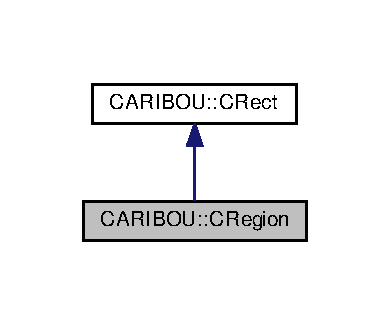
\includegraphics[width=186pt]{class_c_a_r_i_b_o_u_1_1_c_region__inherit__graph}
\end{center}
\end{figure}


Collaboration diagram for C\-A\-R\-I\-B\-O\-U\-:\-:C\-Region\-:\nopagebreak
\begin{figure}[H]
\begin{center}
\leavevmode
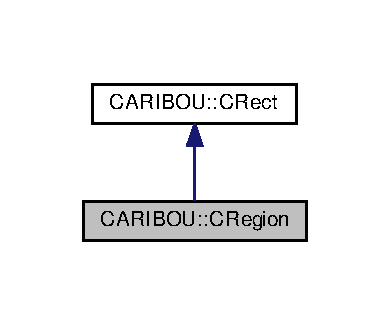
\includegraphics[width=186pt]{class_c_a_r_i_b_o_u_1_1_c_region__coll__graph}
\end{center}
\end{figure}
\subsection*{Public Member Functions}
\begin{DoxyCompactItemize}
\item 
{\bf C\-Region} ()
\item 
{\bf C\-Region} (int16\-\_\-t {\bf x}, int16\-\_\-t {\bf y}, int16\-\_\-t {\bf width}, int16\-\_\-t {\bf height})
\item 
{\bf C\-Region} ({\bf C\-Rect} rect)
\item 
{\bf C\-Region} ({\bf C\-Point} {\bf pos}, {\bf C\-Size} {\bf size})
\item 
{\bf C\-Region} (const {\bf C\-Region} \&other)
\item 
{\bf $\sim$\-C\-Region} ()
\item 
void {\bf append} ({\bf C\-Rect} rect)
\begin{DoxyCompactList}\small\item\em append a rectangle to the region \end{DoxyCompactList}\item 
{\bf C\-Rect} {\bf at} (int {\bf pos})
\item 
int {\bf count} ()
\item 
void {\bf clear} ()
\begin{DoxyCompactList}\small\item\em clear the contained rectangles. \end{DoxyCompactList}\item 
{\bf C\-Region} \& {\bf operator=} (const {\bf C\-Region} \&other)
\end{DoxyCompactItemize}
\subsection*{Protected Member Functions}
\begin{DoxyCompactItemize}
\item 
void {\bf update} ()
\begin{DoxyCompactList}\small\item\em unite all of the contained rectangles to form region bounds. \end{DoxyCompactList}\end{DoxyCompactItemize}
\subsection*{Additional Inherited Members}


\subsection{Detailed Description}
a region is sequence of rectangles 

Definition at line 30 of file cregion.\-h.



\subsection{Constructor \& Destructor Documentation}
\index{C\-A\-R\-I\-B\-O\-U\-::\-C\-Region@{C\-A\-R\-I\-B\-O\-U\-::\-C\-Region}!C\-Region@{C\-Region}}
\index{C\-Region@{C\-Region}!CARIBOU::CRegion@{C\-A\-R\-I\-B\-O\-U\-::\-C\-Region}}
\subsubsection[{C\-Region}]{\setlength{\rightskip}{0pt plus 5cm}C\-A\-R\-I\-B\-O\-U\-::\-C\-Region\-::\-C\-Region (
\begin{DoxyParamCaption}
{}
\end{DoxyParamCaption}
)}\label{class_c_a_r_i_b_o_u_1_1_c_region_a84c352d69acd7ab844e8ba03c66f109e}


Definition at line 23 of file cregion.\-cpp.

\index{C\-A\-R\-I\-B\-O\-U\-::\-C\-Region@{C\-A\-R\-I\-B\-O\-U\-::\-C\-Region}!C\-Region@{C\-Region}}
\index{C\-Region@{C\-Region}!CARIBOU::CRegion@{C\-A\-R\-I\-B\-O\-U\-::\-C\-Region}}
\subsubsection[{C\-Region}]{\setlength{\rightskip}{0pt plus 5cm}C\-A\-R\-I\-B\-O\-U\-::\-C\-Region\-::\-C\-Region (
\begin{DoxyParamCaption}
\item[{int16\-\_\-t}]{x, }
\item[{int16\-\_\-t}]{y, }
\item[{int16\-\_\-t}]{width, }
\item[{int16\-\_\-t}]{height}
\end{DoxyParamCaption}
)}\label{class_c_a_r_i_b_o_u_1_1_c_region_a41882aeff63b877f1ffb07022146d3db}


Definition at line 28 of file cregion.\-cpp.

\index{C\-A\-R\-I\-B\-O\-U\-::\-C\-Region@{C\-A\-R\-I\-B\-O\-U\-::\-C\-Region}!C\-Region@{C\-Region}}
\index{C\-Region@{C\-Region}!CARIBOU::CRegion@{C\-A\-R\-I\-B\-O\-U\-::\-C\-Region}}
\subsubsection[{C\-Region}]{\setlength{\rightskip}{0pt plus 5cm}C\-A\-R\-I\-B\-O\-U\-::\-C\-Region\-::\-C\-Region (
\begin{DoxyParamCaption}
\item[{{\bf C\-Rect}}]{rect}
\end{DoxyParamCaption}
)}\label{class_c_a_r_i_b_o_u_1_1_c_region_ad28789f53a66c49347d53133b4dbe0ec}


Definition at line 33 of file cregion.\-cpp.

\index{C\-A\-R\-I\-B\-O\-U\-::\-C\-Region@{C\-A\-R\-I\-B\-O\-U\-::\-C\-Region}!C\-Region@{C\-Region}}
\index{C\-Region@{C\-Region}!CARIBOU::CRegion@{C\-A\-R\-I\-B\-O\-U\-::\-C\-Region}}
\subsubsection[{C\-Region}]{\setlength{\rightskip}{0pt plus 5cm}C\-A\-R\-I\-B\-O\-U\-::\-C\-Region\-::\-C\-Region (
\begin{DoxyParamCaption}
\item[{{\bf C\-Point}}]{pos, }
\item[{{\bf C\-Size}}]{size}
\end{DoxyParamCaption}
)}\label{class_c_a_r_i_b_o_u_1_1_c_region_a02a0892d502f2a893376d74169a0238f}
\index{C\-A\-R\-I\-B\-O\-U\-::\-C\-Region@{C\-A\-R\-I\-B\-O\-U\-::\-C\-Region}!C\-Region@{C\-Region}}
\index{C\-Region@{C\-Region}!CARIBOU::CRegion@{C\-A\-R\-I\-B\-O\-U\-::\-C\-Region}}
\subsubsection[{C\-Region}]{\setlength{\rightskip}{0pt plus 5cm}C\-A\-R\-I\-B\-O\-U\-::\-C\-Region\-::\-C\-Region (
\begin{DoxyParamCaption}
\item[{const {\bf C\-Region} \&}]{other}
\end{DoxyParamCaption}
)}\label{class_c_a_r_i_b_o_u_1_1_c_region_a16ec4ba618c4fe3b519597968dfd3c12}


Definition at line 38 of file cregion.\-cpp.

\index{C\-A\-R\-I\-B\-O\-U\-::\-C\-Region@{C\-A\-R\-I\-B\-O\-U\-::\-C\-Region}!$\sim$\-C\-Region@{$\sim$\-C\-Region}}
\index{$\sim$\-C\-Region@{$\sim$\-C\-Region}!CARIBOU::CRegion@{C\-A\-R\-I\-B\-O\-U\-::\-C\-Region}}
\subsubsection[{$\sim$\-C\-Region}]{\setlength{\rightskip}{0pt plus 5cm}C\-A\-R\-I\-B\-O\-U\-::\-C\-Region\-::$\sim$\-C\-Region (
\begin{DoxyParamCaption}
{}
\end{DoxyParamCaption}
)}\label{class_c_a_r_i_b_o_u_1_1_c_region_a84f93497ff7da622ad35ccb4a80ec9cb}


Definition at line 48 of file cregion.\-cpp.



\subsection{Member Function Documentation}
\index{C\-A\-R\-I\-B\-O\-U\-::\-C\-Region@{C\-A\-R\-I\-B\-O\-U\-::\-C\-Region}!append@{append}}
\index{append@{append}!CARIBOU::CRegion@{C\-A\-R\-I\-B\-O\-U\-::\-C\-Region}}
\subsubsection[{append}]{\setlength{\rightskip}{0pt plus 5cm}void C\-A\-R\-I\-B\-O\-U\-::\-C\-Region\-::append (
\begin{DoxyParamCaption}
\item[{{\bf C\-Rect}}]{rect}
\end{DoxyParamCaption}
)}\label{class_c_a_r_i_b_o_u_1_1_c_region_aeb12e57f8eeab3d34a78510e9c9afc37}


append a rectangle to the region 



Definition at line 64 of file cregion.\-cpp.

\index{C\-A\-R\-I\-B\-O\-U\-::\-C\-Region@{C\-A\-R\-I\-B\-O\-U\-::\-C\-Region}!at@{at}}
\index{at@{at}!CARIBOU::CRegion@{C\-A\-R\-I\-B\-O\-U\-::\-C\-Region}}
\subsubsection[{at}]{\setlength{\rightskip}{0pt plus 5cm}{\bf C\-Rect} C\-A\-R\-I\-B\-O\-U\-::\-C\-Region\-::at (
\begin{DoxyParamCaption}
\item[{int}]{pos}
\end{DoxyParamCaption}
)}\label{class_c_a_r_i_b_o_u_1_1_c_region_a5f534dd99d4c7e0ed48464657e202a7a}
\begin{DoxyReturn}{Returns}
the rectangle at the position. 
\end{DoxyReturn}


Definition at line 75 of file cregion.\-cpp.

\index{C\-A\-R\-I\-B\-O\-U\-::\-C\-Region@{C\-A\-R\-I\-B\-O\-U\-::\-C\-Region}!clear@{clear}}
\index{clear@{clear}!CARIBOU::CRegion@{C\-A\-R\-I\-B\-O\-U\-::\-C\-Region}}
\subsubsection[{clear}]{\setlength{\rightskip}{0pt plus 5cm}void C\-A\-R\-I\-B\-O\-U\-::\-C\-Region\-::clear (
\begin{DoxyParamCaption}
{}
\end{DoxyParamCaption}
)}\label{class_c_a_r_i_b_o_u_1_1_c_region_a923e12ed661fbcc3ae6156e548061b7f}


clear the contained rectangles. 



Definition at line 93 of file cregion.\-cpp.

\index{C\-A\-R\-I\-B\-O\-U\-::\-C\-Region@{C\-A\-R\-I\-B\-O\-U\-::\-C\-Region}!count@{count}}
\index{count@{count}!CARIBOU::CRegion@{C\-A\-R\-I\-B\-O\-U\-::\-C\-Region}}
\subsubsection[{count}]{\setlength{\rightskip}{0pt plus 5cm}int C\-A\-R\-I\-B\-O\-U\-::\-C\-Region\-::count (
\begin{DoxyParamCaption}
{}
\end{DoxyParamCaption}
)}\label{class_c_a_r_i_b_o_u_1_1_c_region_a17b40b248536452e09f8e738417715ab}
\begin{DoxyReturn}{Returns}
the number of rectangles in the region 
\end{DoxyReturn}


Definition at line 87 of file cregion.\-cpp.

\index{C\-A\-R\-I\-B\-O\-U\-::\-C\-Region@{C\-A\-R\-I\-B\-O\-U\-::\-C\-Region}!operator=@{operator=}}
\index{operator=@{operator=}!CARIBOU::CRegion@{C\-A\-R\-I\-B\-O\-U\-::\-C\-Region}}
\subsubsection[{operator=}]{\setlength{\rightskip}{0pt plus 5cm}{\bf C\-Region} \& C\-A\-R\-I\-B\-O\-U\-::\-C\-Region\-::operator= (
\begin{DoxyParamCaption}
\item[{const {\bf C\-Region} \&}]{other}
\end{DoxyParamCaption}
)}\label{class_c_a_r_i_b_o_u_1_1_c_region_a7e9130bc740d258a0177158b17b1de88}


Definition at line 53 of file cregion.\-cpp.

\index{C\-A\-R\-I\-B\-O\-U\-::\-C\-Region@{C\-A\-R\-I\-B\-O\-U\-::\-C\-Region}!update@{update}}
\index{update@{update}!CARIBOU::CRegion@{C\-A\-R\-I\-B\-O\-U\-::\-C\-Region}}
\subsubsection[{update}]{\setlength{\rightskip}{0pt plus 5cm}void C\-A\-R\-I\-B\-O\-U\-::\-C\-Region\-::update (
\begin{DoxyParamCaption}
{}
\end{DoxyParamCaption}
)\hspace{0.3cm}{\ttfamily [protected]}}\label{class_c_a_r_i_b_o_u_1_1_c_region_a25c3b6a140a22e9b4a28255cd288d71b}


unite all of the contained rectangles to form region bounds. 



Definition at line 101 of file cregion.\-cpp.



The documentation for this class was generated from the following files\-:\begin{DoxyCompactItemize}
\item 
include/caribou++/{\bf cregion.\-h}\item 
src/{\bf cregion.\-cpp}\end{DoxyCompactItemize}

\section{C\-A\-R\-I\-B\-O\-U\-:\-:C\-Ring\-Buffer Class Reference}
\label{class_c_a_r_i_b_o_u_1_1_c_ring_buffer}\index{C\-A\-R\-I\-B\-O\-U\-::\-C\-Ring\-Buffer@{C\-A\-R\-I\-B\-O\-U\-::\-C\-Ring\-Buffer}}


Implements a ring buffer of bytes.  




{\ttfamily \#include $<$cringbuffer.\-h$>$}



Inheritance diagram for C\-A\-R\-I\-B\-O\-U\-:\-:C\-Ring\-Buffer\-:\nopagebreak
\begin{figure}[H]
\begin{center}
\leavevmode
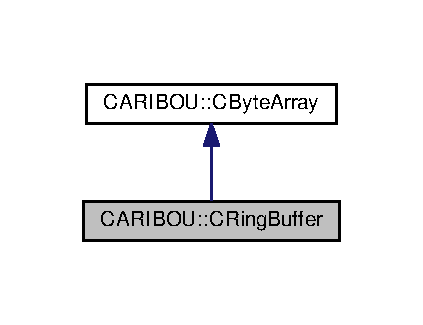
\includegraphics[width=202pt]{class_c_a_r_i_b_o_u_1_1_c_ring_buffer__inherit__graph}
\end{center}
\end{figure}


Collaboration diagram for C\-A\-R\-I\-B\-O\-U\-:\-:C\-Ring\-Buffer\-:\nopagebreak
\begin{figure}[H]
\begin{center}
\leavevmode
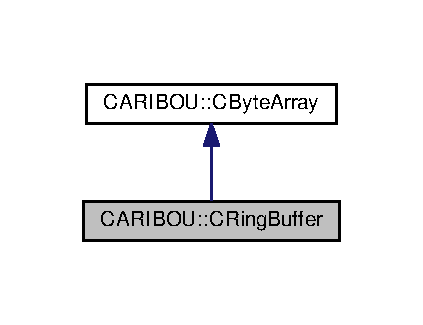
\includegraphics[width=202pt]{class_c_a_r_i_b_o_u_1_1_c_ring_buffer__coll__graph}
\end{center}
\end{figure}
\subsection*{Public Member Functions}
\begin{DoxyCompactItemize}
\item 
{\bf C\-Ring\-Buffer} ()
\item 
{\bf $\sim$\-C\-Ring\-Buffer} ()
\item 
virtual size\-\_\-t {\bf resize} (size\-\_\-t {\bf size})
\begin{DoxyCompactList}\small\item\em resize taking into account existing data. \end{DoxyCompactList}\item 
virtual void {\bf clear} ()
\item 
size\-\_\-t {\bf insert} (uint8\-\_\-t ch)
\begin{DoxyCompactList}\small\item\em insert a character into the ring buffer, advancing the head. \end{DoxyCompactList}\item 
size\-\_\-t {\bf insert} ({\bf C\-Byte\-Array} \&bytes)
\begin{DoxyCompactList}\small\item\em insert a character into the ring buffer, advancing the head. \end{DoxyCompactList}\item 
uint8\-\_\-t {\bf peek} ()
\begin{DoxyCompactList}\small\item\em Peek at the next character in the ring buffer but do not remove it. \end{DoxyCompactList}\item 
uint8\-\_\-t {\bf remove} ()
\begin{DoxyCompactList}\small\item\em Remove the next character from the ring buffer. \end{DoxyCompactList}\item 
uint8\-\_\-t {\bf remove} (uint8\-\_\-t ch)
\begin{DoxyCompactList}\small\item\em Remove the next character from the ring buffer and insert a new one. \end{DoxyCompactList}\item 
size\-\_\-t {\bf length} ()
\begin{DoxyCompactList}\small\item\em Determin the length of the data contained in the ring buffer taking wrap around into account. \end{DoxyCompactList}\item 
bool {\bf full} ()
\item 
uint16\-\_\-t {\bf free} ()
\item 
bool {\bf empty} ()
\item 
uint16\-\_\-t {\bf overflow} ()
\item 
{\bf C\-Byte\-Array} {\bf to\-Byte\-Array} ()
\begin{DoxyCompactList}\small\item\em Convert the contents of the ring buffer into a byte array in the order the bytes where recieved. \end{DoxyCompactList}\end{DoxyCompactItemize}
\subsection*{Additional Inherited Members}


\subsection{Detailed Description}
Implements a ring buffer of bytes. 

\begin{DoxyAuthor}{Author}
Michael Sharkey {\tt mike@pikeaero.\-com} 
\end{DoxyAuthor}


Definition at line 28 of file cringbuffer.\-h.



\subsection{Constructor \& Destructor Documentation}
\index{C\-A\-R\-I\-B\-O\-U\-::\-C\-Ring\-Buffer@{C\-A\-R\-I\-B\-O\-U\-::\-C\-Ring\-Buffer}!C\-Ring\-Buffer@{C\-Ring\-Buffer}}
\index{C\-Ring\-Buffer@{C\-Ring\-Buffer}!CARIBOU::CRingBuffer@{C\-A\-R\-I\-B\-O\-U\-::\-C\-Ring\-Buffer}}
\subsubsection[{C\-Ring\-Buffer}]{\setlength{\rightskip}{0pt plus 5cm}C\-A\-R\-I\-B\-O\-U\-::\-C\-Ring\-Buffer\-::\-C\-Ring\-Buffer (
\begin{DoxyParamCaption}
{}
\end{DoxyParamCaption}
)}\label{class_c_a_r_i_b_o_u_1_1_c_ring_buffer_a538c43fdc6d79f403409b0aba17074b9}


Definition at line 23 of file cringbuffer.\-cpp.

\index{C\-A\-R\-I\-B\-O\-U\-::\-C\-Ring\-Buffer@{C\-A\-R\-I\-B\-O\-U\-::\-C\-Ring\-Buffer}!$\sim$\-C\-Ring\-Buffer@{$\sim$\-C\-Ring\-Buffer}}
\index{$\sim$\-C\-Ring\-Buffer@{$\sim$\-C\-Ring\-Buffer}!CARIBOU::CRingBuffer@{C\-A\-R\-I\-B\-O\-U\-::\-C\-Ring\-Buffer}}
\subsubsection[{$\sim$\-C\-Ring\-Buffer}]{\setlength{\rightskip}{0pt plus 5cm}C\-A\-R\-I\-B\-O\-U\-::\-C\-Ring\-Buffer\-::$\sim$\-C\-Ring\-Buffer (
\begin{DoxyParamCaption}
{}
\end{DoxyParamCaption}
)}\label{class_c_a_r_i_b_o_u_1_1_c_ring_buffer_a2d0debeb007803df7430056d06e309de}


Definition at line 31 of file cringbuffer.\-cpp.



\subsection{Member Function Documentation}
\index{C\-A\-R\-I\-B\-O\-U\-::\-C\-Ring\-Buffer@{C\-A\-R\-I\-B\-O\-U\-::\-C\-Ring\-Buffer}!clear@{clear}}
\index{clear@{clear}!CARIBOU::CRingBuffer@{C\-A\-R\-I\-B\-O\-U\-::\-C\-Ring\-Buffer}}
\subsubsection[{clear}]{\setlength{\rightskip}{0pt plus 5cm}virtual void C\-A\-R\-I\-B\-O\-U\-::\-C\-Ring\-Buffer\-::clear (
\begin{DoxyParamCaption}
{}
\end{DoxyParamCaption}
)\hspace{0.3cm}{\ttfamily [inline]}, {\ttfamily [virtual]}}\label{class_c_a_r_i_b_o_u_1_1_c_ring_buffer_acf387649e99034ef25a6fb5cd40edd3a}


Reimplemented from {\bf C\-A\-R\-I\-B\-O\-U\-::\-C\-Byte\-Array} \doxyref{}{p.}{class_c_a_r_i_b_o_u_1_1_c_byte_array_a21a6406374c2f76a71e3a1f038dbf31a}.



Definition at line 35 of file cringbuffer.\-h.

\index{C\-A\-R\-I\-B\-O\-U\-::\-C\-Ring\-Buffer@{C\-A\-R\-I\-B\-O\-U\-::\-C\-Ring\-Buffer}!empty@{empty}}
\index{empty@{empty}!CARIBOU::CRingBuffer@{C\-A\-R\-I\-B\-O\-U\-::\-C\-Ring\-Buffer}}
\subsubsection[{empty}]{\setlength{\rightskip}{0pt plus 5cm}bool C\-A\-R\-I\-B\-O\-U\-::\-C\-Ring\-Buffer\-::empty (
\begin{DoxyParamCaption}
{}
\end{DoxyParamCaption}
)\hspace{0.3cm}{\ttfamily [inline]}}\label{class_c_a_r_i_b_o_u_1_1_c_ring_buffer_a7c794fd6ce9a33aa4b88fec7ffd5416b}


Definition at line 44 of file cringbuffer.\-h.

\index{C\-A\-R\-I\-B\-O\-U\-::\-C\-Ring\-Buffer@{C\-A\-R\-I\-B\-O\-U\-::\-C\-Ring\-Buffer}!free@{free}}
\index{free@{free}!CARIBOU::CRingBuffer@{C\-A\-R\-I\-B\-O\-U\-::\-C\-Ring\-Buffer}}
\subsubsection[{free}]{\setlength{\rightskip}{0pt plus 5cm}uint16\-\_\-t C\-A\-R\-I\-B\-O\-U\-::\-C\-Ring\-Buffer\-::free (
\begin{DoxyParamCaption}
{}
\end{DoxyParamCaption}
)\hspace{0.3cm}{\ttfamily [inline]}}\label{class_c_a_r_i_b_o_u_1_1_c_ring_buffer_ae6833e8430f88ce9832ea093a9916b73}


Definition at line 43 of file cringbuffer.\-h.

\index{C\-A\-R\-I\-B\-O\-U\-::\-C\-Ring\-Buffer@{C\-A\-R\-I\-B\-O\-U\-::\-C\-Ring\-Buffer}!full@{full}}
\index{full@{full}!CARIBOU::CRingBuffer@{C\-A\-R\-I\-B\-O\-U\-::\-C\-Ring\-Buffer}}
\subsubsection[{full}]{\setlength{\rightskip}{0pt plus 5cm}bool C\-A\-R\-I\-B\-O\-U\-::\-C\-Ring\-Buffer\-::full (
\begin{DoxyParamCaption}
{}
\end{DoxyParamCaption}
)\hspace{0.3cm}{\ttfamily [inline]}}\label{class_c_a_r_i_b_o_u_1_1_c_ring_buffer_a4154537450771ec1d56de689d8686b52}


Definition at line 42 of file cringbuffer.\-h.

\index{C\-A\-R\-I\-B\-O\-U\-::\-C\-Ring\-Buffer@{C\-A\-R\-I\-B\-O\-U\-::\-C\-Ring\-Buffer}!insert@{insert}}
\index{insert@{insert}!CARIBOU::CRingBuffer@{C\-A\-R\-I\-B\-O\-U\-::\-C\-Ring\-Buffer}}
\subsubsection[{insert}]{\setlength{\rightskip}{0pt plus 5cm}size\-\_\-t C\-A\-R\-I\-B\-O\-U\-::\-C\-Ring\-Buffer\-::insert (
\begin{DoxyParamCaption}
\item[{uint8\-\_\-t}]{ch}
\end{DoxyParamCaption}
)}\label{class_c_a_r_i_b_o_u_1_1_c_ring_buffer_aa6d130853dc4175a5b29240253c38b78}


insert a character into the ring buffer, advancing the head. 

\begin{DoxyReturn}{Returns}
1 if there was room, else 0 
\end{DoxyReturn}


Definition at line 69 of file cringbuffer.\-cpp.

\index{C\-A\-R\-I\-B\-O\-U\-::\-C\-Ring\-Buffer@{C\-A\-R\-I\-B\-O\-U\-::\-C\-Ring\-Buffer}!insert@{insert}}
\index{insert@{insert}!CARIBOU::CRingBuffer@{C\-A\-R\-I\-B\-O\-U\-::\-C\-Ring\-Buffer}}
\subsubsection[{insert}]{\setlength{\rightskip}{0pt plus 5cm}size\-\_\-t C\-A\-R\-I\-B\-O\-U\-::\-C\-Ring\-Buffer\-::insert (
\begin{DoxyParamCaption}
\item[{{\bf C\-Byte\-Array} \&}]{bytes}
\end{DoxyParamCaption}
)}\label{class_c_a_r_i_b_o_u_1_1_c_ring_buffer_a81d219c23ecea6eea00301e888a9282e}


insert a character into the ring buffer, advancing the head. 

\begin{DoxyReturn}{Returns}
1 if there was room, else 0 
\end{DoxyReturn}


Definition at line 88 of file cringbuffer.\-cpp.

\index{C\-A\-R\-I\-B\-O\-U\-::\-C\-Ring\-Buffer@{C\-A\-R\-I\-B\-O\-U\-::\-C\-Ring\-Buffer}!length@{length}}
\index{length@{length}!CARIBOU::CRingBuffer@{C\-A\-R\-I\-B\-O\-U\-::\-C\-Ring\-Buffer}}
\subsubsection[{length}]{\setlength{\rightskip}{0pt plus 5cm}size\-\_\-t C\-A\-R\-I\-B\-O\-U\-::\-C\-Ring\-Buffer\-::length (
\begin{DoxyParamCaption}
{}
\end{DoxyParamCaption}
)\hspace{0.3cm}{\ttfamily [virtual]}}\label{class_c_a_r_i_b_o_u_1_1_c_ring_buffer_a0912316591e34c5d6d608397e89f1475}


Determin the length of the data contained in the ring buffer taking wrap around into account. 

\begin{DoxyReturn}{Returns}
The length of the contents of the ring buffer. 
\end{DoxyReturn}


Reimplemented from {\bf C\-A\-R\-I\-B\-O\-U\-::\-C\-Byte\-Array} \doxyref{}{p.}{class_c_a_r_i_b_o_u_1_1_c_byte_array_ad15b129f7a5169d87c90b9ec14a7f285}.



Definition at line 144 of file cringbuffer.\-cpp.

\index{C\-A\-R\-I\-B\-O\-U\-::\-C\-Ring\-Buffer@{C\-A\-R\-I\-B\-O\-U\-::\-C\-Ring\-Buffer}!overflow@{overflow}}
\index{overflow@{overflow}!CARIBOU::CRingBuffer@{C\-A\-R\-I\-B\-O\-U\-::\-C\-Ring\-Buffer}}
\subsubsection[{overflow}]{\setlength{\rightskip}{0pt plus 5cm}uint16\-\_\-t C\-A\-R\-I\-B\-O\-U\-::\-C\-Ring\-Buffer\-::overflow (
\begin{DoxyParamCaption}
{}
\end{DoxyParamCaption}
)\hspace{0.3cm}{\ttfamily [inline]}}\label{class_c_a_r_i_b_o_u_1_1_c_ring_buffer_a42c3a4372b08e3928554ce8f1b6770a0}


Definition at line 45 of file cringbuffer.\-h.

\index{C\-A\-R\-I\-B\-O\-U\-::\-C\-Ring\-Buffer@{C\-A\-R\-I\-B\-O\-U\-::\-C\-Ring\-Buffer}!peek@{peek}}
\index{peek@{peek}!CARIBOU::CRingBuffer@{C\-A\-R\-I\-B\-O\-U\-::\-C\-Ring\-Buffer}}
\subsubsection[{peek}]{\setlength{\rightskip}{0pt plus 5cm}uint8\-\_\-t C\-A\-R\-I\-B\-O\-U\-::\-C\-Ring\-Buffer\-::peek (
\begin{DoxyParamCaption}
{}
\end{DoxyParamCaption}
)}\label{class_c_a_r_i_b_o_u_1_1_c_ring_buffer_a99124d6ce9d279f0cecedd92138dae63}


Peek at the next character in the ring buffer but do not remove it. 

\begin{DoxyReturn}{Returns}
the character. 
\end{DoxyReturn}


Definition at line 103 of file cringbuffer.\-cpp.

\index{C\-A\-R\-I\-B\-O\-U\-::\-C\-Ring\-Buffer@{C\-A\-R\-I\-B\-O\-U\-::\-C\-Ring\-Buffer}!remove@{remove}}
\index{remove@{remove}!CARIBOU::CRingBuffer@{C\-A\-R\-I\-B\-O\-U\-::\-C\-Ring\-Buffer}}
\subsubsection[{remove}]{\setlength{\rightskip}{0pt plus 5cm}uint8\-\_\-t C\-A\-R\-I\-B\-O\-U\-::\-C\-Ring\-Buffer\-::remove (
\begin{DoxyParamCaption}
{}
\end{DoxyParamCaption}
)}\label{class_c_a_r_i_b_o_u_1_1_c_ring_buffer_a11902e2a6c1412a72dc9739e5f7dc7e4}


Remove the next character from the ring buffer. 

\begin{DoxyReturn}{Returns}
the character 
\end{DoxyReturn}


Definition at line 114 of file cringbuffer.\-cpp.

\index{C\-A\-R\-I\-B\-O\-U\-::\-C\-Ring\-Buffer@{C\-A\-R\-I\-B\-O\-U\-::\-C\-Ring\-Buffer}!remove@{remove}}
\index{remove@{remove}!CARIBOU::CRingBuffer@{C\-A\-R\-I\-B\-O\-U\-::\-C\-Ring\-Buffer}}
\subsubsection[{remove}]{\setlength{\rightskip}{0pt plus 5cm}uint8\-\_\-t C\-A\-R\-I\-B\-O\-U\-::\-C\-Ring\-Buffer\-::remove (
\begin{DoxyParamCaption}
\item[{uint8\-\_\-t}]{ch}
\end{DoxyParamCaption}
)}\label{class_c_a_r_i_b_o_u_1_1_c_ring_buffer_a6aef1b66329587005d46930115d8a283}


Remove the next character from the ring buffer and insert a new one. 

\begin{DoxyReturn}{Returns}
the removed character 
\end{DoxyReturn}


Definition at line 133 of file cringbuffer.\-cpp.

\index{C\-A\-R\-I\-B\-O\-U\-::\-C\-Ring\-Buffer@{C\-A\-R\-I\-B\-O\-U\-::\-C\-Ring\-Buffer}!resize@{resize}}
\index{resize@{resize}!CARIBOU::CRingBuffer@{C\-A\-R\-I\-B\-O\-U\-::\-C\-Ring\-Buffer}}
\subsubsection[{resize}]{\setlength{\rightskip}{0pt plus 5cm}size\-\_\-t C\-A\-R\-I\-B\-O\-U\-::\-C\-Ring\-Buffer\-::resize (
\begin{DoxyParamCaption}
\item[{size\-\_\-t}]{size}
\end{DoxyParamCaption}
)\hspace{0.3cm}{\ttfamily [virtual]}}\label{class_c_a_r_i_b_o_u_1_1_c_ring_buffer_a2802c6bc5f7bd6eb460f970d18676700}


resize taking into account existing data. 

If resizing smaller, data may be lost. \begin{DoxyReturn}{Returns}
a self reference 
\end{DoxyReturn}


Reimplemented from {\bf C\-A\-R\-I\-B\-O\-U\-::\-C\-Byte\-Array} \doxyref{}{p.}{class_c_a_r_i_b_o_u_1_1_c_byte_array_ad9a01a668ed71959fe1539dd77b9223e}.



Definition at line 39 of file cringbuffer.\-cpp.

\index{C\-A\-R\-I\-B\-O\-U\-::\-C\-Ring\-Buffer@{C\-A\-R\-I\-B\-O\-U\-::\-C\-Ring\-Buffer}!to\-Byte\-Array@{to\-Byte\-Array}}
\index{to\-Byte\-Array@{to\-Byte\-Array}!CARIBOU::CRingBuffer@{C\-A\-R\-I\-B\-O\-U\-::\-C\-Ring\-Buffer}}
\subsubsection[{to\-Byte\-Array}]{\setlength{\rightskip}{0pt plus 5cm}{\bf C\-Byte\-Array} C\-A\-R\-I\-B\-O\-U\-::\-C\-Ring\-Buffer\-::to\-Byte\-Array (
\begin{DoxyParamCaption}
{}
\end{DoxyParamCaption}
)}\label{class_c_a_r_i_b_o_u_1_1_c_ring_buffer_a0d9522519a948347a8548cc2a24abe35}


Convert the contents of the ring buffer into a byte array in the order the bytes where recieved. 



Definition at line 161 of file cringbuffer.\-cpp.



The documentation for this class was generated from the following files\-:\begin{DoxyCompactItemize}
\item 
include/caribou++/{\bf cringbuffer.\-h}\item 
src/{\bf cringbuffer.\-cpp}\end{DoxyCompactItemize}

\section{C\+A\+R\+I\+B\+OU\+:\+:C\+Semaphore Class Reference}
\label{class_c_a_r_i_b_o_u_1_1_c_semaphore}\index{C\+A\+R\+I\+B\+O\+U\+::\+C\+Semaphore@{C\+A\+R\+I\+B\+O\+U\+::\+C\+Semaphore}}


{\ttfamily \#include $<$csemaphore.\+h$>$}

\subsection*{Public Member Functions}
\begin{DoxyCompactItemize}
\item 
{\bf C\+Semaphore} (int count)
\item 
{\bf C\+Semaphore} (const {\bf C\+Semaphore} \&other)
\item 
virtual {\bf $\sim$\+C\+Semaphore} ()
\item 
{\bf C\+Semaphore} \& {\bf operator=} (const {\bf C\+Semaphore} \&other)
\item 
bool {\bf signal} ()
\item 
bool {\bf wait} (caribou\+\_\+tick\+\_\+t timeout=T\+I\+M\+E\+O\+U\+T\+\_\+\+I\+N\+F\+I\+N\+I\+TE)
\item 
bool {\bf try\+Wait} ()
\end{DoxyCompactItemize}


\subsection{Detailed Description}


Definition at line 27 of file csemaphore.\+h.



\subsection{Constructor \& Destructor Documentation}
\index{C\+A\+R\+I\+B\+O\+U\+::\+C\+Semaphore@{C\+A\+R\+I\+B\+O\+U\+::\+C\+Semaphore}!C\+Semaphore@{C\+Semaphore}}
\index{C\+Semaphore@{C\+Semaphore}!C\+A\+R\+I\+B\+O\+U\+::\+C\+Semaphore@{C\+A\+R\+I\+B\+O\+U\+::\+C\+Semaphore}}
\subsubsection[{C\+Semaphore(int count)}]{\setlength{\rightskip}{0pt plus 5cm}C\+A\+R\+I\+B\+O\+U\+::\+C\+Semaphore\+::\+C\+Semaphore (
\begin{DoxyParamCaption}
\item[{int}]{count}
\end{DoxyParamCaption}
)}\label{class_c_a_r_i_b_o_u_1_1_c_semaphore_a885fd2e0710a23cef88892af235ae1a9}


Definition at line 23 of file csemaphore.\+cpp.

\index{C\+A\+R\+I\+B\+O\+U\+::\+C\+Semaphore@{C\+A\+R\+I\+B\+O\+U\+::\+C\+Semaphore}!C\+Semaphore@{C\+Semaphore}}
\index{C\+Semaphore@{C\+Semaphore}!C\+A\+R\+I\+B\+O\+U\+::\+C\+Semaphore@{C\+A\+R\+I\+B\+O\+U\+::\+C\+Semaphore}}
\subsubsection[{C\+Semaphore(const C\+Semaphore \&other)}]{\setlength{\rightskip}{0pt plus 5cm}C\+A\+R\+I\+B\+O\+U\+::\+C\+Semaphore\+::\+C\+Semaphore (
\begin{DoxyParamCaption}
\item[{const {\bf C\+Semaphore} \&}]{other}
\end{DoxyParamCaption}
)}\label{class_c_a_r_i_b_o_u_1_1_c_semaphore_aa12c41a3b44788943dbffa9f2b5fdb3a}


Definition at line 28 of file csemaphore.\+cpp.

\index{C\+A\+R\+I\+B\+O\+U\+::\+C\+Semaphore@{C\+A\+R\+I\+B\+O\+U\+::\+C\+Semaphore}!````~C\+Semaphore@{$\sim$\+C\+Semaphore}}
\index{````~C\+Semaphore@{$\sim$\+C\+Semaphore}!C\+A\+R\+I\+B\+O\+U\+::\+C\+Semaphore@{C\+A\+R\+I\+B\+O\+U\+::\+C\+Semaphore}}
\subsubsection[{$\sim$\+C\+Semaphore()}]{\setlength{\rightskip}{0pt plus 5cm}C\+A\+R\+I\+B\+O\+U\+::\+C\+Semaphore\+::$\sim$\+C\+Semaphore (
\begin{DoxyParamCaption}
{}
\end{DoxyParamCaption}
)\hspace{0.3cm}{\ttfamily [virtual]}}\label{class_c_a_r_i_b_o_u_1_1_c_semaphore_a5ca2b7f6b52b63d9b4f9c6ab307a322e}


Definition at line 36 of file csemaphore.\+cpp.



\subsection{Member Function Documentation}
\index{C\+A\+R\+I\+B\+O\+U\+::\+C\+Semaphore@{C\+A\+R\+I\+B\+O\+U\+::\+C\+Semaphore}!operator=@{operator=}}
\index{operator=@{operator=}!C\+A\+R\+I\+B\+O\+U\+::\+C\+Semaphore@{C\+A\+R\+I\+B\+O\+U\+::\+C\+Semaphore}}
\subsubsection[{operator=(const C\+Semaphore \&other)}]{\setlength{\rightskip}{0pt plus 5cm}{\bf C\+Semaphore} \& C\+A\+R\+I\+B\+O\+U\+::\+C\+Semaphore\+::operator= (
\begin{DoxyParamCaption}
\item[{const {\bf C\+Semaphore} \&}]{other}
\end{DoxyParamCaption}
)}\label{class_c_a_r_i_b_o_u_1_1_c_semaphore_aaa968e248eeb7426118fbb526d06d297}


Definition at line 41 of file csemaphore.\+cpp.

\index{C\+A\+R\+I\+B\+O\+U\+::\+C\+Semaphore@{C\+A\+R\+I\+B\+O\+U\+::\+C\+Semaphore}!signal@{signal}}
\index{signal@{signal}!C\+A\+R\+I\+B\+O\+U\+::\+C\+Semaphore@{C\+A\+R\+I\+B\+O\+U\+::\+C\+Semaphore}}
\subsubsection[{signal()}]{\setlength{\rightskip}{0pt plus 5cm}bool C\+A\+R\+I\+B\+O\+U\+::\+C\+Semaphore\+::signal (
\begin{DoxyParamCaption}
{}
\end{DoxyParamCaption}
)}\label{class_c_a_r_i_b_o_u_1_1_c_semaphore_a204bfffac2b3f6afa13a72f3d4d58260}


Definition at line 46 of file csemaphore.\+cpp.

\index{C\+A\+R\+I\+B\+O\+U\+::\+C\+Semaphore@{C\+A\+R\+I\+B\+O\+U\+::\+C\+Semaphore}!try\+Wait@{try\+Wait}}
\index{try\+Wait@{try\+Wait}!C\+A\+R\+I\+B\+O\+U\+::\+C\+Semaphore@{C\+A\+R\+I\+B\+O\+U\+::\+C\+Semaphore}}
\subsubsection[{try\+Wait()}]{\setlength{\rightskip}{0pt plus 5cm}bool C\+A\+R\+I\+B\+O\+U\+::\+C\+Semaphore\+::try\+Wait (
\begin{DoxyParamCaption}
{}
\end{DoxyParamCaption}
)}\label{class_c_a_r_i_b_o_u_1_1_c_semaphore_a9a1d46913d87ae4161ccf00f1793579b}


Definition at line 56 of file csemaphore.\+cpp.

\index{C\+A\+R\+I\+B\+O\+U\+::\+C\+Semaphore@{C\+A\+R\+I\+B\+O\+U\+::\+C\+Semaphore}!wait@{wait}}
\index{wait@{wait}!C\+A\+R\+I\+B\+O\+U\+::\+C\+Semaphore@{C\+A\+R\+I\+B\+O\+U\+::\+C\+Semaphore}}
\subsubsection[{wait(caribou\+\_\+tick\+\_\+t timeout=\+T\+I\+M\+E\+O\+U\+T\+\_\+\+I\+N\+F\+I\+N\+I\+T\+E)}]{\setlength{\rightskip}{0pt plus 5cm}bool C\+A\+R\+I\+B\+O\+U\+::\+C\+Semaphore\+::wait (
\begin{DoxyParamCaption}
\item[{caribou\+\_\+tick\+\_\+t}]{timeout = {\ttfamily TIMEOUT\+\_\+INFINITE}}
\end{DoxyParamCaption}
)}\label{class_c_a_r_i_b_o_u_1_1_c_semaphore_a7e7b688ae33168a7b5cb32d04af32406}


Definition at line 51 of file csemaphore.\+cpp.



The documentation for this class was generated from the following files\+:\begin{DoxyCompactItemize}
\item 
include/caribou++/{\bf csemaphore.\+h}\item 
src/{\bf csemaphore.\+cpp}\end{DoxyCompactItemize}

\section{C\-A\-R\-I\-B\-O\-U\-:\-:C\-S\-H\-A1 Class Reference}
\label{class_c_a_r_i_b_o_u_1_1_c_s_h_a1}\index{C\-A\-R\-I\-B\-O\-U\-::\-C\-S\-H\-A1@{C\-A\-R\-I\-B\-O\-U\-::\-C\-S\-H\-A1}}


{\ttfamily \#include $<$csha1.\-h$>$}

\subsection*{Public Member Functions}
\begin{DoxyCompactItemize}
\item 
{\bf C\-S\-H\-A1} ()
\item 
{\bf C\-S\-H\-A1} (const {\bf C\-A\-R\-I\-B\-O\-U\-::\-C\-Byte\-Array} cleartext)
\item 
{\bf $\sim$\-C\-S\-H\-A1} ()
\item 
void {\bf reset} ()
\begin{DoxyCompactList}\small\item\em initialize in preparation for computing a new message digest \end{DoxyCompactList}\item 
void {\bf input} (const uint8\-\_\-t $\ast$message, size\-\_\-t size)
\begin{DoxyCompactList}\small\item\em This function accepts octets as the next portion of the message. \end{DoxyCompactList}\item 
void {\bf input} ({\bf C\-A\-R\-I\-B\-O\-U\-::\-C\-Byte\-Array} message)
\begin{DoxyCompactList}\small\item\em This function accepts octets as the next portion of the message. \end{DoxyCompactList}\item 
{\bf C\-A\-R\-I\-B\-O\-U\-::\-C\-Byte\-Array} {\bf result} ()
\item 
{\bf C\-A\-R\-I\-B\-O\-U\-::\-C\-String} {\bf hex\-Result} ()
\end{DoxyCompactItemize}


\subsection{Detailed Description}


Definition at line 24 of file csha1.\-h.



\subsection{Constructor \& Destructor Documentation}
\index{C\-A\-R\-I\-B\-O\-U\-::\-C\-S\-H\-A1@{C\-A\-R\-I\-B\-O\-U\-::\-C\-S\-H\-A1}!C\-S\-H\-A1@{C\-S\-H\-A1}}
\index{C\-S\-H\-A1@{C\-S\-H\-A1}!CARIBOU::CSHA1@{C\-A\-R\-I\-B\-O\-U\-::\-C\-S\-H\-A1}}
\subsubsection[{C\-S\-H\-A1}]{\setlength{\rightskip}{0pt plus 5cm}C\-A\-R\-I\-B\-O\-U\-::\-C\-S\-H\-A1\-::\-C\-S\-H\-A1 (
\begin{DoxyParamCaption}
{}
\end{DoxyParamCaption}
)}\label{class_c_a_r_i_b_o_u_1_1_c_s_h_a1_abf3d12d09ad4d75d13495a30c1dd00c1}


Definition at line 18 of file csha1.\-cpp.

\index{C\-A\-R\-I\-B\-O\-U\-::\-C\-S\-H\-A1@{C\-A\-R\-I\-B\-O\-U\-::\-C\-S\-H\-A1}!C\-S\-H\-A1@{C\-S\-H\-A1}}
\index{C\-S\-H\-A1@{C\-S\-H\-A1}!CARIBOU::CSHA1@{C\-A\-R\-I\-B\-O\-U\-::\-C\-S\-H\-A1}}
\subsubsection[{C\-S\-H\-A1}]{\setlength{\rightskip}{0pt plus 5cm}C\-A\-R\-I\-B\-O\-U\-::\-C\-S\-H\-A1\-::\-C\-S\-H\-A1 (
\begin{DoxyParamCaption}
\item[{const {\bf C\-A\-R\-I\-B\-O\-U\-::\-C\-Byte\-Array}}]{cleartext}
\end{DoxyParamCaption}
)}\label{class_c_a_r_i_b_o_u_1_1_c_s_h_a1_a228746abfd65b5107e3ad407f5bedb8a}


Definition at line 23 of file csha1.\-cpp.

\index{C\-A\-R\-I\-B\-O\-U\-::\-C\-S\-H\-A1@{C\-A\-R\-I\-B\-O\-U\-::\-C\-S\-H\-A1}!$\sim$\-C\-S\-H\-A1@{$\sim$\-C\-S\-H\-A1}}
\index{$\sim$\-C\-S\-H\-A1@{$\sim$\-C\-S\-H\-A1}!CARIBOU::CSHA1@{C\-A\-R\-I\-B\-O\-U\-::\-C\-S\-H\-A1}}
\subsubsection[{$\sim$\-C\-S\-H\-A1}]{\setlength{\rightskip}{0pt plus 5cm}C\-A\-R\-I\-B\-O\-U\-::\-C\-S\-H\-A1\-::$\sim$\-C\-S\-H\-A1 (
\begin{DoxyParamCaption}
{}
\end{DoxyParamCaption}
)}\label{class_c_a_r_i_b_o_u_1_1_c_s_h_a1_a814ff0873baba5c62f13fb76f4f0b79c}


Definition at line 29 of file csha1.\-cpp.



\subsection{Member Function Documentation}
\index{C\-A\-R\-I\-B\-O\-U\-::\-C\-S\-H\-A1@{C\-A\-R\-I\-B\-O\-U\-::\-C\-S\-H\-A1}!hex\-Result@{hex\-Result}}
\index{hex\-Result@{hex\-Result}!CARIBOU::CSHA1@{C\-A\-R\-I\-B\-O\-U\-::\-C\-S\-H\-A1}}
\subsubsection[{hex\-Result}]{\setlength{\rightskip}{0pt plus 5cm}{\bf C\-A\-R\-I\-B\-O\-U\-::\-C\-String} C\-A\-R\-I\-B\-O\-U\-::\-C\-S\-H\-A1\-::hex\-Result (
\begin{DoxyParamCaption}
{}
\end{DoxyParamCaption}
)}\label{class_c_a_r_i_b_o_u_1_1_c_s_h_a1_adbea01a3608cff78c33d88107afc103e}


Definition at line 76 of file csha1.\-cpp.

\index{C\-A\-R\-I\-B\-O\-U\-::\-C\-S\-H\-A1@{C\-A\-R\-I\-B\-O\-U\-::\-C\-S\-H\-A1}!input@{input}}
\index{input@{input}!CARIBOU::CSHA1@{C\-A\-R\-I\-B\-O\-U\-::\-C\-S\-H\-A1}}
\subsubsection[{input}]{\setlength{\rightskip}{0pt plus 5cm}void C\-A\-R\-I\-B\-O\-U\-::\-C\-S\-H\-A1\-::input (
\begin{DoxyParamCaption}
\item[{const uint8\-\_\-t $\ast$}]{message, }
\item[{size\-\_\-t}]{size}
\end{DoxyParamCaption}
)}\label{class_c_a_r_i_b_o_u_1_1_c_s_h_a1_a0b516216b6b878c23037fb15d2adbf41}


This function accepts octets as the next portion of the message. 



Definition at line 86 of file csha1.\-cpp.

\index{C\-A\-R\-I\-B\-O\-U\-::\-C\-S\-H\-A1@{C\-A\-R\-I\-B\-O\-U\-::\-C\-S\-H\-A1}!input@{input}}
\index{input@{input}!CARIBOU::CSHA1@{C\-A\-R\-I\-B\-O\-U\-::\-C\-S\-H\-A1}}
\subsubsection[{input}]{\setlength{\rightskip}{0pt plus 5cm}void C\-A\-R\-I\-B\-O\-U\-::\-C\-S\-H\-A1\-::input (
\begin{DoxyParamCaption}
\item[{{\bf C\-A\-R\-I\-B\-O\-U\-::\-C\-Byte\-Array}}]{message}
\end{DoxyParamCaption}
)}\label{class_c_a_r_i_b_o_u_1_1_c_s_h_a1_a3b16b6283bf740ed7f1b3a3f34f8f679}


This function accepts octets as the next portion of the message. 



Definition at line 125 of file csha1.\-cpp.

\index{C\-A\-R\-I\-B\-O\-U\-::\-C\-S\-H\-A1@{C\-A\-R\-I\-B\-O\-U\-::\-C\-S\-H\-A1}!reset@{reset}}
\index{reset@{reset}!CARIBOU::CSHA1@{C\-A\-R\-I\-B\-O\-U\-::\-C\-S\-H\-A1}}
\subsubsection[{reset}]{\setlength{\rightskip}{0pt plus 5cm}void C\-A\-R\-I\-B\-O\-U\-::\-C\-S\-H\-A1\-::reset (
\begin{DoxyParamCaption}
{}
\end{DoxyParamCaption}
)}\label{class_c_a_r_i_b_o_u_1_1_c_s_h_a1_a26758a1ca55449bc106307a281d1b5a0}


initialize in preparation for computing a new message digest 



Definition at line 36 of file csha1.\-cpp.

\index{C\-A\-R\-I\-B\-O\-U\-::\-C\-S\-H\-A1@{C\-A\-R\-I\-B\-O\-U\-::\-C\-S\-H\-A1}!result@{result}}
\index{result@{result}!CARIBOU::CSHA1@{C\-A\-R\-I\-B\-O\-U\-::\-C\-S\-H\-A1}}
\subsubsection[{result}]{\setlength{\rightskip}{0pt plus 5cm}{\bf C\-A\-R\-I\-B\-O\-U\-::\-C\-Byte\-Array} C\-A\-R\-I\-B\-O\-U\-::\-C\-S\-H\-A1\-::result (
\begin{DoxyParamCaption}
{}
\end{DoxyParamCaption}
)}\label{class_c_a_r_i_b_o_u_1_1_c_s_h_a1_a16493646d80142484d8b435d269fc43e}


Definition at line 53 of file csha1.\-cpp.



The documentation for this class was generated from the following files\-:\begin{DoxyCompactItemize}
\item 
include/caribou++/{\bf csha1.\-h}\item 
src/{\bf csha1.\-cpp}\end{DoxyCompactItemize}

\section{C\-A\-R\-I\-B\-O\-U\-:\-:C\-Size Class Reference}
\label{class_c_a_r_i_b_o_u_1_1_c_size}\index{C\-A\-R\-I\-B\-O\-U\-::\-C\-Size@{C\-A\-R\-I\-B\-O\-U\-::\-C\-Size}}


{\ttfamily \#include $<$csize.\-h$>$}

\subsection*{Public Member Functions}
\begin{DoxyCompactItemize}
\item 
{\bf C\-Size} ()
\item 
{\bf C\-Size} (const {\bf C\-Size} \&other)
\item 
{\bf C\-Size} (int16\-\_\-t {\bf width}, int16\-\_\-t {\bf height})
\item 
{\bf $\sim$\-C\-Size} ()
\item 
void {\bf clear} ()
\item 
void {\bf copy} (const {\bf C\-Size} \&other)
\item 
void {\bf resize} ({\bf C\-Size} size)
\item 
void {\bf resize} (int16\-\_\-t w, int16\-\_\-t h)
\item 
void {\bf set\-Width} (int16\-\_\-t w)
\item 
void {\bf set\-Height} (int16\-\_\-t h)
\item 
int16\-\_\-t {\bf width} ()
\item 
int16\-\_\-t {\bf height} ()
\item 
{\bf C\-Size} \& {\bf add} (const {\bf C\-Size} \&other)
\begin{DoxyCompactList}\small\item\em Add an offset from another point. \end{DoxyCompactList}\item 
{\bf C\-Size} \& {\bf subtract} (const {\bf C\-Size} \&other)
\begin{DoxyCompactList}\small\item\em Subtract an offset from another point. \end{DoxyCompactList}\item 
bool {\bf is\-Empty} ()
\item 
{\bf C\-Size} \& {\bf operator=} (const {\bf C\-Size} \&other)
\item 
{\bf C\-Size} \& {\bf operator+=} (const {\bf C\-Size} \&other)
\item 
{\bf C\-Size} \& {\bf operator-\/=} (const {\bf C\-Size} \&other)
\item 
bool {\bf operator==} (const {\bf C\-Size} \&other)
\item 
bool {\bf operator!=} (const {\bf C\-Size} \&other)
\end{DoxyCompactItemize}


\subsection{Detailed Description}


Definition at line 24 of file csize.\-h.



\subsection{Constructor \& Destructor Documentation}
\index{C\-A\-R\-I\-B\-O\-U\-::\-C\-Size@{C\-A\-R\-I\-B\-O\-U\-::\-C\-Size}!C\-Size@{C\-Size}}
\index{C\-Size@{C\-Size}!CARIBOU::CSize@{C\-A\-R\-I\-B\-O\-U\-::\-C\-Size}}
\subsubsection[{C\-Size}]{\setlength{\rightskip}{0pt plus 5cm}C\-A\-R\-I\-B\-O\-U\-::\-C\-Size\-::\-C\-Size (
\begin{DoxyParamCaption}
{}
\end{DoxyParamCaption}
)}\label{class_c_a_r_i_b_o_u_1_1_c_size_a333b1114c0cb8a95e3cf590e8e724292}


Definition at line 21 of file csize.\-cpp.

\index{C\-A\-R\-I\-B\-O\-U\-::\-C\-Size@{C\-A\-R\-I\-B\-O\-U\-::\-C\-Size}!C\-Size@{C\-Size}}
\index{C\-Size@{C\-Size}!CARIBOU::CSize@{C\-A\-R\-I\-B\-O\-U\-::\-C\-Size}}
\subsubsection[{C\-Size}]{\setlength{\rightskip}{0pt plus 5cm}C\-A\-R\-I\-B\-O\-U\-::\-C\-Size\-::\-C\-Size (
\begin{DoxyParamCaption}
\item[{const {\bf C\-Size} \&}]{other}
\end{DoxyParamCaption}
)}\label{class_c_a_r_i_b_o_u_1_1_c_size_afab9e9978b0bd4b7937fe62b0dff083f}


Definition at line 27 of file csize.\-cpp.

\index{C\-A\-R\-I\-B\-O\-U\-::\-C\-Size@{C\-A\-R\-I\-B\-O\-U\-::\-C\-Size}!C\-Size@{C\-Size}}
\index{C\-Size@{C\-Size}!CARIBOU::CSize@{C\-A\-R\-I\-B\-O\-U\-::\-C\-Size}}
\subsubsection[{C\-Size}]{\setlength{\rightskip}{0pt plus 5cm}C\-A\-R\-I\-B\-O\-U\-::\-C\-Size\-::\-C\-Size (
\begin{DoxyParamCaption}
\item[{int16\-\_\-t}]{width, }
\item[{int16\-\_\-t}]{height}
\end{DoxyParamCaption}
)}\label{class_c_a_r_i_b_o_u_1_1_c_size_a1725e39f4d745132437737e740915b06}


Definition at line 33 of file csize.\-cpp.

\index{C\-A\-R\-I\-B\-O\-U\-::\-C\-Size@{C\-A\-R\-I\-B\-O\-U\-::\-C\-Size}!$\sim$\-C\-Size@{$\sim$\-C\-Size}}
\index{$\sim$\-C\-Size@{$\sim$\-C\-Size}!CARIBOU::CSize@{C\-A\-R\-I\-B\-O\-U\-::\-C\-Size}}
\subsubsection[{$\sim$\-C\-Size}]{\setlength{\rightskip}{0pt plus 5cm}C\-A\-R\-I\-B\-O\-U\-::\-C\-Size\-::$\sim$\-C\-Size (
\begin{DoxyParamCaption}
{}
\end{DoxyParamCaption}
)}\label{class_c_a_r_i_b_o_u_1_1_c_size_aa13c81b71b7ebc47b620d5ac22d15809}


Definition at line 39 of file csize.\-cpp.



\subsection{Member Function Documentation}
\index{C\-A\-R\-I\-B\-O\-U\-::\-C\-Size@{C\-A\-R\-I\-B\-O\-U\-::\-C\-Size}!add@{add}}
\index{add@{add}!CARIBOU::CSize@{C\-A\-R\-I\-B\-O\-U\-::\-C\-Size}}
\subsubsection[{add}]{\setlength{\rightskip}{0pt plus 5cm}{\bf C\-Size} \& C\-A\-R\-I\-B\-O\-U\-::\-C\-Size\-::add (
\begin{DoxyParamCaption}
\item[{const {\bf C\-Size} \&}]{other}
\end{DoxyParamCaption}
)}\label{class_c_a_r_i_b_o_u_1_1_c_size_a30dcf8a984391d960b6c65b5d988afcf}


Add an offset from another point. 



Definition at line 46 of file csize.\-cpp.

\index{C\-A\-R\-I\-B\-O\-U\-::\-C\-Size@{C\-A\-R\-I\-B\-O\-U\-::\-C\-Size}!clear@{clear}}
\index{clear@{clear}!CARIBOU::CSize@{C\-A\-R\-I\-B\-O\-U\-::\-C\-Size}}
\subsubsection[{clear}]{\setlength{\rightskip}{0pt plus 5cm}void C\-A\-R\-I\-B\-O\-U\-::\-C\-Size\-::clear (
\begin{DoxyParamCaption}
{}
\end{DoxyParamCaption}
)\hspace{0.3cm}{\ttfamily [inline]}}\label{class_c_a_r_i_b_o_u_1_1_c_size_a1df86aa6eec69f5ebba3e04771e64ca3}


Definition at line 32 of file csize.\-h.

\index{C\-A\-R\-I\-B\-O\-U\-::\-C\-Size@{C\-A\-R\-I\-B\-O\-U\-::\-C\-Size}!copy@{copy}}
\index{copy@{copy}!CARIBOU::CSize@{C\-A\-R\-I\-B\-O\-U\-::\-C\-Size}}
\subsubsection[{copy}]{\setlength{\rightskip}{0pt plus 5cm}void C\-A\-R\-I\-B\-O\-U\-::\-C\-Size\-::copy (
\begin{DoxyParamCaption}
\item[{const {\bf C\-Size} \&}]{other}
\end{DoxyParamCaption}
)\hspace{0.3cm}{\ttfamily [inline]}}\label{class_c_a_r_i_b_o_u_1_1_c_size_ab511740d26d706671741a9aa8ab71d2b}


Definition at line 33 of file csize.\-h.

\index{C\-A\-R\-I\-B\-O\-U\-::\-C\-Size@{C\-A\-R\-I\-B\-O\-U\-::\-C\-Size}!height@{height}}
\index{height@{height}!CARIBOU::CSize@{C\-A\-R\-I\-B\-O\-U\-::\-C\-Size}}
\subsubsection[{height}]{\setlength{\rightskip}{0pt plus 5cm}int16\-\_\-t C\-A\-R\-I\-B\-O\-U\-::\-C\-Size\-::height (
\begin{DoxyParamCaption}
{}
\end{DoxyParamCaption}
)\hspace{0.3cm}{\ttfamily [inline]}}\label{class_c_a_r_i_b_o_u_1_1_c_size_a5351d795e043d78a4388e4f13fa45321}


Definition at line 40 of file csize.\-h.

\index{C\-A\-R\-I\-B\-O\-U\-::\-C\-Size@{C\-A\-R\-I\-B\-O\-U\-::\-C\-Size}!is\-Empty@{is\-Empty}}
\index{is\-Empty@{is\-Empty}!CARIBOU::CSize@{C\-A\-R\-I\-B\-O\-U\-::\-C\-Size}}
\subsubsection[{is\-Empty}]{\setlength{\rightskip}{0pt plus 5cm}bool C\-A\-R\-I\-B\-O\-U\-::\-C\-Size\-::is\-Empty (
\begin{DoxyParamCaption}
{}
\end{DoxyParamCaption}
)\hspace{0.3cm}{\ttfamily [inline]}}\label{class_c_a_r_i_b_o_u_1_1_c_size_aac446e13300ef90f84fc1f14b82d8433}


Definition at line 45 of file csize.\-h.

\index{C\-A\-R\-I\-B\-O\-U\-::\-C\-Size@{C\-A\-R\-I\-B\-O\-U\-::\-C\-Size}!operator!=@{operator!=}}
\index{operator!=@{operator!=}!CARIBOU::CSize@{C\-A\-R\-I\-B\-O\-U\-::\-C\-Size}}
\subsubsection[{operator!=}]{\setlength{\rightskip}{0pt plus 5cm}bool C\-A\-R\-I\-B\-O\-U\-::\-C\-Size\-::operator!= (
\begin{DoxyParamCaption}
\item[{const {\bf C\-Size} \&}]{other}
\end{DoxyParamCaption}
)}\label{class_c_a_r_i_b_o_u_1_1_c_size_ad5398fb219858d372aec94be311c4963}


Definition at line 86 of file csize.\-cpp.

\index{C\-A\-R\-I\-B\-O\-U\-::\-C\-Size@{C\-A\-R\-I\-B\-O\-U\-::\-C\-Size}!operator+=@{operator+=}}
\index{operator+=@{operator+=}!CARIBOU::CSize@{C\-A\-R\-I\-B\-O\-U\-::\-C\-Size}}
\subsubsection[{operator+=}]{\setlength{\rightskip}{0pt plus 5cm}{\bf C\-Size} \& C\-A\-R\-I\-B\-O\-U\-::\-C\-Size\-::operator+= (
\begin{DoxyParamCaption}
\item[{const {\bf C\-Size} \&}]{other}
\end{DoxyParamCaption}
)}\label{class_c_a_r_i_b_o_u_1_1_c_size_aa27ea46db270ae7c205e7624fec751ee}


Definition at line 70 of file csize.\-cpp.

\index{C\-A\-R\-I\-B\-O\-U\-::\-C\-Size@{C\-A\-R\-I\-B\-O\-U\-::\-C\-Size}!operator-\/=@{operator-\/=}}
\index{operator-\/=@{operator-\/=}!CARIBOU::CSize@{C\-A\-R\-I\-B\-O\-U\-::\-C\-Size}}
\subsubsection[{operator-\/=}]{\setlength{\rightskip}{0pt plus 5cm}{\bf C\-Size} \& C\-A\-R\-I\-B\-O\-U\-::\-C\-Size\-::operator-\/= (
\begin{DoxyParamCaption}
\item[{const {\bf C\-Size} \&}]{other}
\end{DoxyParamCaption}
)}\label{class_c_a_r_i_b_o_u_1_1_c_size_a86bb56b3830ed77c0d976dee7160a685}


Definition at line 75 of file csize.\-cpp.

\index{C\-A\-R\-I\-B\-O\-U\-::\-C\-Size@{C\-A\-R\-I\-B\-O\-U\-::\-C\-Size}!operator=@{operator=}}
\index{operator=@{operator=}!CARIBOU::CSize@{C\-A\-R\-I\-B\-O\-U\-::\-C\-Size}}
\subsubsection[{operator=}]{\setlength{\rightskip}{0pt plus 5cm}{\bf C\-Size} \& C\-A\-R\-I\-B\-O\-U\-::\-C\-Size\-::operator= (
\begin{DoxyParamCaption}
\item[{const {\bf C\-Size} \&}]{other}
\end{DoxyParamCaption}
)}\label{class_c_a_r_i_b_o_u_1_1_c_size_aff0e3093ad7446365a78100151507d1b}


Definition at line 63 of file csize.\-cpp.

\index{C\-A\-R\-I\-B\-O\-U\-::\-C\-Size@{C\-A\-R\-I\-B\-O\-U\-::\-C\-Size}!operator==@{operator==}}
\index{operator==@{operator==}!CARIBOU::CSize@{C\-A\-R\-I\-B\-O\-U\-::\-C\-Size}}
\subsubsection[{operator==}]{\setlength{\rightskip}{0pt plus 5cm}bool C\-A\-R\-I\-B\-O\-U\-::\-C\-Size\-::operator== (
\begin{DoxyParamCaption}
\item[{const {\bf C\-Size} \&}]{other}
\end{DoxyParamCaption}
)}\label{class_c_a_r_i_b_o_u_1_1_c_size_ad3fae347b9d0a01929e9229647a1b7e0}


Definition at line 80 of file csize.\-cpp.

\index{C\-A\-R\-I\-B\-O\-U\-::\-C\-Size@{C\-A\-R\-I\-B\-O\-U\-::\-C\-Size}!resize@{resize}}
\index{resize@{resize}!CARIBOU::CSize@{C\-A\-R\-I\-B\-O\-U\-::\-C\-Size}}
\subsubsection[{resize}]{\setlength{\rightskip}{0pt plus 5cm}void C\-A\-R\-I\-B\-O\-U\-::\-C\-Size\-::resize (
\begin{DoxyParamCaption}
\item[{{\bf C\-Size}}]{size}
\end{DoxyParamCaption}
)\hspace{0.3cm}{\ttfamily [inline]}}\label{class_c_a_r_i_b_o_u_1_1_c_size_a8a02d889074caec2a2ca8045195fb8a8}


Definition at line 34 of file csize.\-h.

\index{C\-A\-R\-I\-B\-O\-U\-::\-C\-Size@{C\-A\-R\-I\-B\-O\-U\-::\-C\-Size}!resize@{resize}}
\index{resize@{resize}!CARIBOU::CSize@{C\-A\-R\-I\-B\-O\-U\-::\-C\-Size}}
\subsubsection[{resize}]{\setlength{\rightskip}{0pt plus 5cm}void C\-A\-R\-I\-B\-O\-U\-::\-C\-Size\-::resize (
\begin{DoxyParamCaption}
\item[{int16\-\_\-t}]{w, }
\item[{int16\-\_\-t}]{h}
\end{DoxyParamCaption}
)\hspace{0.3cm}{\ttfamily [inline]}}\label{class_c_a_r_i_b_o_u_1_1_c_size_aac37b4b92dd23350b7ead38685ea70fa}


Definition at line 35 of file csize.\-h.

\index{C\-A\-R\-I\-B\-O\-U\-::\-C\-Size@{C\-A\-R\-I\-B\-O\-U\-::\-C\-Size}!set\-Height@{set\-Height}}
\index{set\-Height@{set\-Height}!CARIBOU::CSize@{C\-A\-R\-I\-B\-O\-U\-::\-C\-Size}}
\subsubsection[{set\-Height}]{\setlength{\rightskip}{0pt plus 5cm}void C\-A\-R\-I\-B\-O\-U\-::\-C\-Size\-::set\-Height (
\begin{DoxyParamCaption}
\item[{int16\-\_\-t}]{h}
\end{DoxyParamCaption}
)\hspace{0.3cm}{\ttfamily [inline]}}\label{class_c_a_r_i_b_o_u_1_1_c_size_ae27b40481de2ded3d90e03f0ea3f45ab}


Definition at line 37 of file csize.\-h.

\index{C\-A\-R\-I\-B\-O\-U\-::\-C\-Size@{C\-A\-R\-I\-B\-O\-U\-::\-C\-Size}!set\-Width@{set\-Width}}
\index{set\-Width@{set\-Width}!CARIBOU::CSize@{C\-A\-R\-I\-B\-O\-U\-::\-C\-Size}}
\subsubsection[{set\-Width}]{\setlength{\rightskip}{0pt plus 5cm}void C\-A\-R\-I\-B\-O\-U\-::\-C\-Size\-::set\-Width (
\begin{DoxyParamCaption}
\item[{int16\-\_\-t}]{w}
\end{DoxyParamCaption}
)\hspace{0.3cm}{\ttfamily [inline]}}\label{class_c_a_r_i_b_o_u_1_1_c_size_a28a8d3827fae10c63e209d88dc80eef4}


Definition at line 36 of file csize.\-h.

\index{C\-A\-R\-I\-B\-O\-U\-::\-C\-Size@{C\-A\-R\-I\-B\-O\-U\-::\-C\-Size}!subtract@{subtract}}
\index{subtract@{subtract}!CARIBOU::CSize@{C\-A\-R\-I\-B\-O\-U\-::\-C\-Size}}
\subsubsection[{subtract}]{\setlength{\rightskip}{0pt plus 5cm}{\bf C\-Size} \& C\-A\-R\-I\-B\-O\-U\-::\-C\-Size\-::subtract (
\begin{DoxyParamCaption}
\item[{const {\bf C\-Size} \&}]{other}
\end{DoxyParamCaption}
)}\label{class_c_a_r_i_b_o_u_1_1_c_size_a8a73c5a27944efacae0a1cbbfc39f873}


Subtract an offset from another point. 



Definition at line 56 of file csize.\-cpp.

\index{C\-A\-R\-I\-B\-O\-U\-::\-C\-Size@{C\-A\-R\-I\-B\-O\-U\-::\-C\-Size}!width@{width}}
\index{width@{width}!CARIBOU::CSize@{C\-A\-R\-I\-B\-O\-U\-::\-C\-Size}}
\subsubsection[{width}]{\setlength{\rightskip}{0pt plus 5cm}int16\-\_\-t C\-A\-R\-I\-B\-O\-U\-::\-C\-Size\-::width (
\begin{DoxyParamCaption}
{}
\end{DoxyParamCaption}
)\hspace{0.3cm}{\ttfamily [inline]}}\label{class_c_a_r_i_b_o_u_1_1_c_size_adba9f081b0c8dbc05582036b5c86101c}


Definition at line 39 of file csize.\-h.



The documentation for this class was generated from the following files\-:\begin{DoxyCompactItemize}
\item 
include/caribou++/{\bf csize.\-h}\item 
src/{\bf csize.\-cpp}\end{DoxyCompactItemize}

\section{C\+A\+R\+I\+B\+OU\+:\+:C\+Spin\+Lock Class Reference}
\label{class_c_a_r_i_b_o_u_1_1_c_spin_lock}\index{C\+A\+R\+I\+B\+O\+U\+::\+C\+Spin\+Lock@{C\+A\+R\+I\+B\+O\+U\+::\+C\+Spin\+Lock}}


Implements a spinlock.  




{\ttfamily \#include $<$cspinlock.\+h$>$}

\subsection*{Public Member Functions}
\begin{DoxyCompactItemize}
\item 
{\bf C\+Spin\+Lock} (bool {\bf lock}=false)
\item 
{\bf $\sim$\+C\+Spin\+Lock} ()
\item 
bool {\bf try\+Lock} ()
\item 
bool {\bf lock} ()
\item 
bool {\bf unlock} ()
\end{DoxyCompactItemize}


\subsection{Detailed Description}
Implements a spinlock. 

\begin{DoxyAuthor}{Author}
Michael Sharkey {\tt mike@pikeaero.\+com} 
\end{DoxyAuthor}


Definition at line 28 of file cspinlock.\+h.



\subsection{Constructor \& Destructor Documentation}
\index{C\+A\+R\+I\+B\+O\+U\+::\+C\+Spin\+Lock@{C\+A\+R\+I\+B\+O\+U\+::\+C\+Spin\+Lock}!C\+Spin\+Lock@{C\+Spin\+Lock}}
\index{C\+Spin\+Lock@{C\+Spin\+Lock}!C\+A\+R\+I\+B\+O\+U\+::\+C\+Spin\+Lock@{C\+A\+R\+I\+B\+O\+U\+::\+C\+Spin\+Lock}}
\subsubsection[{C\+Spin\+Lock(bool lock=false)}]{\setlength{\rightskip}{0pt plus 5cm}C\+A\+R\+I\+B\+O\+U\+::\+C\+Spin\+Lock\+::\+C\+Spin\+Lock (
\begin{DoxyParamCaption}
\item[{bool}]{lock = {\ttfamily false}}
\end{DoxyParamCaption}
)}\label{class_c_a_r_i_b_o_u_1_1_c_spin_lock_a9fab21c519908f93c49facff12a17de1}


Definition at line 21 of file cspinlock.\+cpp.

\index{C\+A\+R\+I\+B\+O\+U\+::\+C\+Spin\+Lock@{C\+A\+R\+I\+B\+O\+U\+::\+C\+Spin\+Lock}!````~C\+Spin\+Lock@{$\sim$\+C\+Spin\+Lock}}
\index{````~C\+Spin\+Lock@{$\sim$\+C\+Spin\+Lock}!C\+A\+R\+I\+B\+O\+U\+::\+C\+Spin\+Lock@{C\+A\+R\+I\+B\+O\+U\+::\+C\+Spin\+Lock}}
\subsubsection[{$\sim$\+C\+Spin\+Lock()}]{\setlength{\rightskip}{0pt plus 5cm}C\+A\+R\+I\+B\+O\+U\+::\+C\+Spin\+Lock\+::$\sim$\+C\+Spin\+Lock (
\begin{DoxyParamCaption}
{}
\end{DoxyParamCaption}
)}\label{class_c_a_r_i_b_o_u_1_1_c_spin_lock_affd547a1204ecf7cb4d2139e9c912d02}


Definition at line 30 of file cspinlock.\+cpp.



\subsection{Member Function Documentation}
\index{C\+A\+R\+I\+B\+O\+U\+::\+C\+Spin\+Lock@{C\+A\+R\+I\+B\+O\+U\+::\+C\+Spin\+Lock}!lock@{lock}}
\index{lock@{lock}!C\+A\+R\+I\+B\+O\+U\+::\+C\+Spin\+Lock@{C\+A\+R\+I\+B\+O\+U\+::\+C\+Spin\+Lock}}
\subsubsection[{lock()}]{\setlength{\rightskip}{0pt plus 5cm}bool C\+A\+R\+I\+B\+O\+U\+::\+C\+Spin\+Lock\+::lock (
\begin{DoxyParamCaption}
{}
\end{DoxyParamCaption}
)\hspace{0.3cm}{\ttfamily [inline]}}\label{class_c_a_r_i_b_o_u_1_1_c_spin_lock_a97acb51999e77ccec5ffaebb3f8aa892}


Definition at line 35 of file cspinlock.\+h.

\index{C\+A\+R\+I\+B\+O\+U\+::\+C\+Spin\+Lock@{C\+A\+R\+I\+B\+O\+U\+::\+C\+Spin\+Lock}!try\+Lock@{try\+Lock}}
\index{try\+Lock@{try\+Lock}!C\+A\+R\+I\+B\+O\+U\+::\+C\+Spin\+Lock@{C\+A\+R\+I\+B\+O\+U\+::\+C\+Spin\+Lock}}
\subsubsection[{try\+Lock()}]{\setlength{\rightskip}{0pt plus 5cm}bool C\+A\+R\+I\+B\+O\+U\+::\+C\+Spin\+Lock\+::try\+Lock (
\begin{DoxyParamCaption}
{}
\end{DoxyParamCaption}
)\hspace{0.3cm}{\ttfamily [inline]}}\label{class_c_a_r_i_b_o_u_1_1_c_spin_lock_acd831f06d74785429679b09f84c08666}


Definition at line 34 of file cspinlock.\+h.

\index{C\+A\+R\+I\+B\+O\+U\+::\+C\+Spin\+Lock@{C\+A\+R\+I\+B\+O\+U\+::\+C\+Spin\+Lock}!unlock@{unlock}}
\index{unlock@{unlock}!C\+A\+R\+I\+B\+O\+U\+::\+C\+Spin\+Lock@{C\+A\+R\+I\+B\+O\+U\+::\+C\+Spin\+Lock}}
\subsubsection[{unlock()}]{\setlength{\rightskip}{0pt plus 5cm}bool C\+A\+R\+I\+B\+O\+U\+::\+C\+Spin\+Lock\+::unlock (
\begin{DoxyParamCaption}
{}
\end{DoxyParamCaption}
)\hspace{0.3cm}{\ttfamily [inline]}}\label{class_c_a_r_i_b_o_u_1_1_c_spin_lock_a8a91f98fe61ddb3e51bfb0d36826e17b}


Definition at line 36 of file cspinlock.\+h.



The documentation for this class was generated from the following files\+:\begin{DoxyCompactItemize}
\item 
include/caribou++/{\bf cspinlock.\+h}\item 
src/{\bf cspinlock.\+cpp}\end{DoxyCompactItemize}

\section{C\+A\+R\+I\+B\+OU\+:\+:C\+String Class Reference}
\label{class_c_a_r_i_b_o_u_1_1_c_string}\index{C\+A\+R\+I\+B\+O\+U\+::\+C\+String@{C\+A\+R\+I\+B\+O\+U\+::\+C\+String}}


{\ttfamily \#include $<$cstring.\+h$>$}



Inheritance diagram for C\+A\+R\+I\+B\+OU\+:\+:C\+String\+:\nopagebreak
\begin{figure}[H]
\begin{center}
\leavevmode
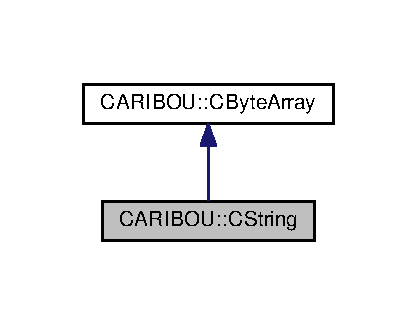
\includegraphics[width=200pt]{class_c_a_r_i_b_o_u_1_1_c_string__inherit__graph}
\end{center}
\end{figure}


Collaboration diagram for C\+A\+R\+I\+B\+OU\+:\+:C\+String\+:\nopagebreak
\begin{figure}[H]
\begin{center}
\leavevmode
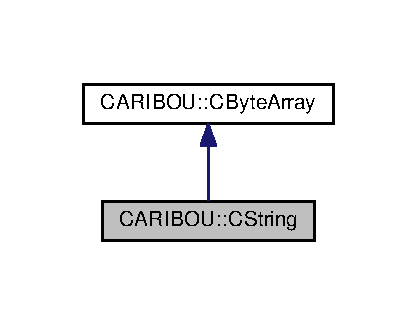
\includegraphics[width=200pt]{class_c_a_r_i_b_o_u_1_1_c_string__coll__graph}
\end{center}
\end{figure}
\subsection*{Public Member Functions}
\begin{DoxyCompactItemize}
\item 
{\bf C\+String} ()
\item 
{\bf C\+String} (const char $\ast$str, int len=-\/1)
\item 
{\bf C\+String} (double f, int dplaces=4, char conv= \textquotesingle{}f\textquotesingle{})
\item 
{\bf C\+String} (const {\bf C\+String} \&other)
\item 
virtual {\bf $\sim$\+C\+String} ()
\item 
virtual size\+\_\+t {\bf resize} (size\+\_\+t {\bf size})
\begin{DoxyCompactList}\small\item\em Resize in terms of usable string characters, transparently maintain terminating null. \end{DoxyCompactList}\item 
bool {\bf append} ({\bf C\+String} \&other)
\item 
bool {\bf append} (const char $\ast${\bf data})
\item 
bool {\bf append} (char ch)
\item 
bool {\bf prepend} (uint8\+\_\+t {\bf data})
\begin{DoxyCompactList}\small\item\em Prepend a character to the string. \end{DoxyCompactList}\item 
bool {\bf prepend} (const char $\ast${\bf data})
\begin{DoxyCompactList}\small\item\em Prepend a chunk of data to the string. \end{DoxyCompactList}\item 
bool {\bf prepend} (const {\bf C\+String} \&{\bf data})
\begin{DoxyCompactList}\small\item\em Prepend a chunk of data to the string. \end{DoxyCompactList}\item 
bool {\bf strcpy} (const char $\ast$s, size\+\_\+t len=0)
\begin{DoxyCompactList}\small\item\em Copies the string pointed to by d, The strings may not overlap. \end{DoxyCompactList}\item 
bool {\bf strcat} (const char $\ast$s, size\+\_\+t len=0)
\begin{DoxyCompactList}\small\item\em The \doxyref{strcat()}{p.}{class_c_a_r_i_b_o_u_1_1_c_string_af30dcb896a9d514cc6ea14b4619fe62b} function appends the d string,The strings may not overlap. \end{DoxyCompactList}\item 
bool {\bf copy} (const char $\ast${\bf data}, int len=-\/1)
\item 
bool {\bf copy} (const {\bf C\+String} \&other)
\item 
int {\bf compare} (const char $\ast$s)
\begin{DoxyCompactList}\small\item\em Compare, taking N\+U\+LL pointers into account. \end{DoxyCompactList}\item 
int {\bf compare} ({\bf C\+String} \&other)
\item 
int {\bf compare} (const char $\ast$s, size\+\_\+t sz)
\item 
int {\bf compare} ({\bf C\+String} \&other, size\+\_\+t sz)
\item 
int {\bf casecompare} (register const char $\ast$s2)
\item 
int {\bf casecompare} ({\bf C\+String} \&other)
\item 
virtual int {\bf find} (char ch, int index=0)
\item 
int {\bf find} (const char $\ast$needle, size\+\_\+t offset=0)
\begin{DoxyCompactList}\small\item\em Find the first occurance of a substring. \end{DoxyCompactList}\item 
int {\bf find} (const {\bf C\+String} \&needle, size\+\_\+t offset=0)
\begin{DoxyCompactList}\small\item\em Find the first occurance of a substring. \end{DoxyCompactList}\item 
{\bf C\+String} \& {\bf replace} (const char $\ast$needle, {\bf C\+String} replacement, size\+\_\+t offset=0)
\begin{DoxyCompactList}\small\item\em Find and replace a substring. \end{DoxyCompactList}\item 
{\bf C\+String} \& {\bf trim} ()
\item 
size\+\_\+t {\bf skip} (const char $\ast$match, size\+\_\+t offset=0)
\item 
{\bf C\+String} \& {\bf operator=} (const {\bf C\+String} \&other)
\item 
{\bf C\+String} \& {\bf operator=} (const char $\ast${\bf data})
\item 
{\bf C\+String} \& {\bf operator=} (const int {\bf data})
\item 
{\bf C\+String} \& {\bf operator=} (const double {\bf data})
\item 
{\bf C\+String} \& {\bf operator+=} ({\bf C\+String} \&other)
\item 
{\bf C\+String} \& {\bf operator+=} (const char $\ast${\bf data})
\item 
{\bf C\+String} \& {\bf operator+=} (char ch)
\item 
bool {\bf operator==} ({\bf C\+String} \&other)
\item 
bool {\bf operator==} (const char $\ast$other)
\item 
bool {\bf operator!=} ({\bf C\+String} \&other)
\item 
bool {\bf operator!=} (const char $\ast$other)
\item 
bool {\bf operator$>$} ({\bf C\+String} \&other)
\item 
bool {\bf operator$>$} (const char $\ast$other)
\item 
bool {\bf operator$<$} ({\bf C\+String} \&other)
\item 
bool {\bf operator$<$} (const char $\ast$other)
\item 
bool {\bf operator$>$=} ({\bf C\+String} \&other)
\item 
bool {\bf operator$>$=} (const char $\ast$other)
\item 
bool {\bf operator$<$=} ({\bf C\+String} \&other)
\item 
bool {\bf operator$<$=} (const char $\ast$other)
\item 
size\+\_\+t {\bf length} ()
\item 
bool {\bf is\+Empty} ()
\item 
bool {\bf is\+Number} ()
\begin{DoxyCompactList}\small\item\em Does the string contain a number? \end{DoxyCompactList}\item 
{\bf C\+String} \& {\bf to\+Lower} ()
\item 
{\bf C\+String} \& {\bf to\+Upper} ()
\item 
{\bf C\+String} {\bf left} (int n)
\item 
{\bf C\+String} {\bf right} (int n)
\item 
{\bf C\+String} {\bf mid} (int index, int n)
\item 
{\bf C\+List}$<$ {\bf C\+String} $\ast$ $>$ {\bf explode} (char separator, int index=0)
\begin{DoxyCompactList}\small\item\em separate a string into substrings based on a separator character. \end{DoxyCompactList}\item 
{\bf C\+String} \& {\bf sprintf} (const char $\ast$fmt,...)
\begin{DoxyCompactList}\small\item\em sprintf( fmt, ... \end{DoxyCompactList}\item 
void {\bf print} (const char $\ast$fmt, va\+\_\+list args)
\begin{DoxyCompactList}\small\item\em sprintf( fmt, ... \end{DoxyCompactList}\item 
{\bf C\+String} \& {\bf from\+U\+Int} (unsigned int i)
\item 
{\bf C\+String} \& {\bf from\+Int} (int i)
\item 
{\bf C\+String} \& {\bf to\+Hex} ({\bf C\+Byte\+Array} bytes)
\item 
{\bf C\+String} \& {\bf to\+Hex} (char $\ast$p, int len)
\item 
{\bf C\+String} \& {\bf to\+Hex} (uint8\+\_\+t n)
\item 
{\bf C\+String} \& {\bf to\+Hex} (uint16\+\_\+t n)
\item 
{\bf C\+String} \& {\bf to\+Hex} (uint32\+\_\+t n)
\item 
{\bf C\+String} \& {\bf to\+Hex} (uint64\+\_\+t n)
\item 
virtual int {\bf to\+Int} ()
\begin{DoxyCompactList}\small\item\em Convert to a signed integer. \end{DoxyCompactList}\item 
virtual unsigned int {\bf to\+U\+Int} ()
\begin{DoxyCompactList}\small\item\em Convert to an unsigned integer. \end{DoxyCompactList}\item 
virtual int64\+\_\+t {\bf to\+Int64} ()
\begin{DoxyCompactList}\small\item\em Convert to a signed integer. \end{DoxyCompactList}\item 
virtual uint64\+\_\+t {\bf to\+U\+Int64} ()
\begin{DoxyCompactList}\small\item\em Convert to an unsigned integer. \end{DoxyCompactList}\item 
virtual bool {\bf to\+Bool} ()
\begin{DoxyCompactList}\small\item\em Convert string to bool. \end{DoxyCompactList}\item 
virtual double {\bf to\+Double} ()
\item 
{\bf C\+String} \& {\bf from\+Bit16} (int16\+\_\+t i, int leading=0)
\begin{DoxyCompactList}\small\item\em Convert an unsigned integer to A\+S\+C\+II in base 10. \end{DoxyCompactList}\item 
{\bf C\+String} \& {\bf from\+Bit32} (int32\+\_\+t i, int leading=0)
\begin{DoxyCompactList}\small\item\em Convert an signed 32-\/bit integer to A\+S\+C\+II in base 10. \end{DoxyCompactList}\item 
{\bf C\+String} \& {\bf from\+Bit64} (int64\+\_\+t i, int leading=0)
\begin{DoxyCompactList}\small\item\em Convert an signed 64-\/bit integer to A\+S\+C\+II in base 10. \end{DoxyCompactList}\item 
{\bf C\+String} \& {\bf from\+U\+Bit32} (uint32\+\_\+t i)
\begin{DoxyCompactList}\small\item\em Convert an unsigned integer to A\+S\+C\+II in base 10. \end{DoxyCompactList}\item 
{\bf C\+String} \& {\bf from\+U\+Bit64} (uint64\+\_\+t i)
\begin{DoxyCompactList}\small\item\em Convert an unsigned long long (aka 64 bit) integer to A\+S\+C\+II in base 10. \end{DoxyCompactList}\item 
{\bf C\+String} \& {\bf from\+Bool} (bool b)
\begin{DoxyCompactList}\small\item\em Convert from bool. \end{DoxyCompactList}\item 
{\bf C\+String} \& {\bf from\+Double} (double d, int dplaces=4, char conv=\textquotesingle{}f\textquotesingle{})
\begin{DoxyCompactList}\small\item\em Converts an I\+E\+EE 754 double precision (32 bit) floating point number to ascii text. \end{DoxyCompactList}\item 
uint32\+\_\+t {\bf from\+Hex} ()
\end{DoxyCompactItemize}
\subsection*{Static Public Member Functions}
\begin{DoxyCompactItemize}
\item 
static {\bf C\+String} {\bf number} (int n)
\item 
static {\bf C\+String} {\bf number} (uint32\+\_\+t n)
\item 
static {\bf C\+String} {\bf number} (uint64\+\_\+t n)
\item 
static {\bf C\+String} {\bf number} (double f, int dplaces=4, char conv= \textquotesingle{}f\textquotesingle{})
\item 
static bool {\bf isalpha} (uint8\+\_\+t c)
\end{DoxyCompactItemize}
\subsection*{Additional Inherited Members}


\subsection{Detailed Description}


Definition at line 26 of file cstring.\+h.



\subsection{Constructor \& Destructor Documentation}
\index{C\+A\+R\+I\+B\+O\+U\+::\+C\+String@{C\+A\+R\+I\+B\+O\+U\+::\+C\+String}!C\+String@{C\+String}}
\index{C\+String@{C\+String}!C\+A\+R\+I\+B\+O\+U\+::\+C\+String@{C\+A\+R\+I\+B\+O\+U\+::\+C\+String}}
\subsubsection[{C\+String()}]{\setlength{\rightskip}{0pt plus 5cm}C\+A\+R\+I\+B\+O\+U\+::\+C\+String\+::\+C\+String (
\begin{DoxyParamCaption}
{}
\end{DoxyParamCaption}
)}\label{class_c_a_r_i_b_o_u_1_1_c_string_aee5777cc68eb028493f441f215bc319e}


Definition at line 25 of file cstring.\+cpp.

\index{C\+A\+R\+I\+B\+O\+U\+::\+C\+String@{C\+A\+R\+I\+B\+O\+U\+::\+C\+String}!C\+String@{C\+String}}
\index{C\+String@{C\+String}!C\+A\+R\+I\+B\+O\+U\+::\+C\+String@{C\+A\+R\+I\+B\+O\+U\+::\+C\+String}}
\subsubsection[{C\+String(const char $\ast$str, int len=-\/1)}]{\setlength{\rightskip}{0pt plus 5cm}C\+A\+R\+I\+B\+O\+U\+::\+C\+String\+::\+C\+String (
\begin{DoxyParamCaption}
\item[{const char $\ast$}]{str, }
\item[{int}]{len = {\ttfamily -\/1}}
\end{DoxyParamCaption}
)}\label{class_c_a_r_i_b_o_u_1_1_c_string_a93bdfa846e2c4f54477397e2038b9d6c}


Definition at line 30 of file cstring.\+cpp.

\index{C\+A\+R\+I\+B\+O\+U\+::\+C\+String@{C\+A\+R\+I\+B\+O\+U\+::\+C\+String}!C\+String@{C\+String}}
\index{C\+String@{C\+String}!C\+A\+R\+I\+B\+O\+U\+::\+C\+String@{C\+A\+R\+I\+B\+O\+U\+::\+C\+String}}
\subsubsection[{C\+String(double f, int dplaces=4, char conv= \textquotesingle{}f\textquotesingle{})}]{\setlength{\rightskip}{0pt plus 5cm}C\+A\+R\+I\+B\+O\+U\+::\+C\+String\+::\+C\+String (
\begin{DoxyParamCaption}
\item[{double}]{f, }
\item[{int}]{dplaces = {\ttfamily 4}, }
\item[{char}]{conv = {\ttfamily \textquotesingle{}f\textquotesingle{}}}
\end{DoxyParamCaption}
)}\label{class_c_a_r_i_b_o_u_1_1_c_string_aae584037dfdf8df81da90b0fad82ba9d}


Definition at line 36 of file cstring.\+cpp.

\index{C\+A\+R\+I\+B\+O\+U\+::\+C\+String@{C\+A\+R\+I\+B\+O\+U\+::\+C\+String}!C\+String@{C\+String}}
\index{C\+String@{C\+String}!C\+A\+R\+I\+B\+O\+U\+::\+C\+String@{C\+A\+R\+I\+B\+O\+U\+::\+C\+String}}
\subsubsection[{C\+String(const C\+String \&other)}]{\setlength{\rightskip}{0pt plus 5cm}C\+A\+R\+I\+B\+O\+U\+::\+C\+String\+::\+C\+String (
\begin{DoxyParamCaption}
\item[{const {\bf C\+String} \&}]{other}
\end{DoxyParamCaption}
)}\label{class_c_a_r_i_b_o_u_1_1_c_string_abeca3c7153b4277baf206978d5ff2040}


Definition at line 42 of file cstring.\+cpp.

\index{C\+A\+R\+I\+B\+O\+U\+::\+C\+String@{C\+A\+R\+I\+B\+O\+U\+::\+C\+String}!````~C\+String@{$\sim$\+C\+String}}
\index{````~C\+String@{$\sim$\+C\+String}!C\+A\+R\+I\+B\+O\+U\+::\+C\+String@{C\+A\+R\+I\+B\+O\+U\+::\+C\+String}}
\subsubsection[{$\sim$\+C\+String()}]{\setlength{\rightskip}{0pt plus 5cm}C\+A\+R\+I\+B\+O\+U\+::\+C\+String\+::$\sim$\+C\+String (
\begin{DoxyParamCaption}
{}
\end{DoxyParamCaption}
)\hspace{0.3cm}{\ttfamily [virtual]}}\label{class_c_a_r_i_b_o_u_1_1_c_string_aba03ef317b796526a7cf28d5395ff56e}


Definition at line 47 of file cstring.\+cpp.



\subsection{Member Function Documentation}
\index{C\+A\+R\+I\+B\+O\+U\+::\+C\+String@{C\+A\+R\+I\+B\+O\+U\+::\+C\+String}!append@{append}}
\index{append@{append}!C\+A\+R\+I\+B\+O\+U\+::\+C\+String@{C\+A\+R\+I\+B\+O\+U\+::\+C\+String}}
\subsubsection[{append(\+C\+String \&other)}]{\setlength{\rightskip}{0pt plus 5cm}bool C\+A\+R\+I\+B\+O\+U\+::\+C\+String\+::append (
\begin{DoxyParamCaption}
\item[{{\bf C\+String} \&}]{other}
\end{DoxyParamCaption}
)}\label{class_c_a_r_i_b_o_u_1_1_c_string_a0d6cfd9aa4f7a39c5f1b53a31729827f}


Definition at line 259 of file cstring.\+cpp.

\index{C\+A\+R\+I\+B\+O\+U\+::\+C\+String@{C\+A\+R\+I\+B\+O\+U\+::\+C\+String}!append@{append}}
\index{append@{append}!C\+A\+R\+I\+B\+O\+U\+::\+C\+String@{C\+A\+R\+I\+B\+O\+U\+::\+C\+String}}
\subsubsection[{append(const char $\ast$data)}]{\setlength{\rightskip}{0pt plus 5cm}bool C\+A\+R\+I\+B\+O\+U\+::\+C\+String\+::append (
\begin{DoxyParamCaption}
\item[{const char $\ast$}]{data}
\end{DoxyParamCaption}
)}\label{class_c_a_r_i_b_o_u_1_1_c_string_a2b7e96cf448d429632027cbb56ad4c48}


Definition at line 264 of file cstring.\+cpp.

\index{C\+A\+R\+I\+B\+O\+U\+::\+C\+String@{C\+A\+R\+I\+B\+O\+U\+::\+C\+String}!append@{append}}
\index{append@{append}!C\+A\+R\+I\+B\+O\+U\+::\+C\+String@{C\+A\+R\+I\+B\+O\+U\+::\+C\+String}}
\subsubsection[{append(char ch)}]{\setlength{\rightskip}{0pt plus 5cm}bool C\+A\+R\+I\+B\+O\+U\+::\+C\+String\+::append (
\begin{DoxyParamCaption}
\item[{char}]{ch}
\end{DoxyParamCaption}
)}\label{class_c_a_r_i_b_o_u_1_1_c_string_a724efb0b5e64b88a8c8876456efa2a4d}


Definition at line 269 of file cstring.\+cpp.

\index{C\+A\+R\+I\+B\+O\+U\+::\+C\+String@{C\+A\+R\+I\+B\+O\+U\+::\+C\+String}!casecompare@{casecompare}}
\index{casecompare@{casecompare}!C\+A\+R\+I\+B\+O\+U\+::\+C\+String@{C\+A\+R\+I\+B\+O\+U\+::\+C\+String}}
\subsubsection[{casecompare(register const char $\ast$s2)}]{\setlength{\rightskip}{0pt plus 5cm}int C\+A\+R\+I\+B\+O\+U\+::\+C\+String\+::casecompare (
\begin{DoxyParamCaption}
\item[{register const char $\ast$}]{s2}
\end{DoxyParamCaption}
)}\label{class_c_a_r_i_b_o_u_1_1_c_string_a998f2bd6c0fc47611f2698abaec6c906}


Definition at line 68 of file cstring.\+cpp.

\index{C\+A\+R\+I\+B\+O\+U\+::\+C\+String@{C\+A\+R\+I\+B\+O\+U\+::\+C\+String}!casecompare@{casecompare}}
\index{casecompare@{casecompare}!C\+A\+R\+I\+B\+O\+U\+::\+C\+String@{C\+A\+R\+I\+B\+O\+U\+::\+C\+String}}
\subsubsection[{casecompare(\+C\+String \&other)}]{\setlength{\rightskip}{0pt plus 5cm}int C\+A\+R\+I\+B\+O\+U\+::\+C\+String\+::casecompare (
\begin{DoxyParamCaption}
\item[{{\bf C\+String} \&}]{other}
\end{DoxyParamCaption}
)}\label{class_c_a_r_i_b_o_u_1_1_c_string_a74ae6c59439828c3e6a5e896d1126686}


Definition at line 86 of file cstring.\+cpp.

\index{C\+A\+R\+I\+B\+O\+U\+::\+C\+String@{C\+A\+R\+I\+B\+O\+U\+::\+C\+String}!compare@{compare}}
\index{compare@{compare}!C\+A\+R\+I\+B\+O\+U\+::\+C\+String@{C\+A\+R\+I\+B\+O\+U\+::\+C\+String}}
\subsubsection[{compare(const char $\ast$s)}]{\setlength{\rightskip}{0pt plus 5cm}int C\+A\+R\+I\+B\+O\+U\+::\+C\+String\+::compare (
\begin{DoxyParamCaption}
\item[{const char $\ast$}]{s}
\end{DoxyParamCaption}
)}\label{class_c_a_r_i_b_o_u_1_1_c_string_a248cf8e88da7cfec63f7a39b0219ee4c}


Compare, taking N\+U\+LL pointers into account. 



Definition at line 94 of file cstring.\+cpp.

\index{C\+A\+R\+I\+B\+O\+U\+::\+C\+String@{C\+A\+R\+I\+B\+O\+U\+::\+C\+String}!compare@{compare}}
\index{compare@{compare}!C\+A\+R\+I\+B\+O\+U\+::\+C\+String@{C\+A\+R\+I\+B\+O\+U\+::\+C\+String}}
\subsubsection[{compare(\+C\+String \&other)}]{\setlength{\rightskip}{0pt plus 5cm}int C\+A\+R\+I\+B\+O\+U\+::\+C\+String\+::compare (
\begin{DoxyParamCaption}
\item[{{\bf C\+String} \&}]{other}
\end{DoxyParamCaption}
)}\label{class_c_a_r_i_b_o_u_1_1_c_string_a44b2431a2bd288964dcd4a57cd87591a}


Definition at line 111 of file cstring.\+cpp.

\index{C\+A\+R\+I\+B\+O\+U\+::\+C\+String@{C\+A\+R\+I\+B\+O\+U\+::\+C\+String}!compare@{compare}}
\index{compare@{compare}!C\+A\+R\+I\+B\+O\+U\+::\+C\+String@{C\+A\+R\+I\+B\+O\+U\+::\+C\+String}}
\subsubsection[{compare(const char $\ast$s, size\+\_\+t sz)}]{\setlength{\rightskip}{0pt plus 5cm}int C\+A\+R\+I\+B\+O\+U\+::\+C\+String\+::compare (
\begin{DoxyParamCaption}
\item[{const char $\ast$}]{s, }
\item[{size\+\_\+t}]{sz}
\end{DoxyParamCaption}
)}\label{class_c_a_r_i_b_o_u_1_1_c_string_a08f25f340f2a71d16b605ac895690353}


Definition at line 116 of file cstring.\+cpp.

\index{C\+A\+R\+I\+B\+O\+U\+::\+C\+String@{C\+A\+R\+I\+B\+O\+U\+::\+C\+String}!compare@{compare}}
\index{compare@{compare}!C\+A\+R\+I\+B\+O\+U\+::\+C\+String@{C\+A\+R\+I\+B\+O\+U\+::\+C\+String}}
\subsubsection[{compare(\+C\+String \&other, size\+\_\+t sz)}]{\setlength{\rightskip}{0pt plus 5cm}int C\+A\+R\+I\+B\+O\+U\+::\+C\+String\+::compare (
\begin{DoxyParamCaption}
\item[{{\bf C\+String} \&}]{other, }
\item[{size\+\_\+t}]{sz}
\end{DoxyParamCaption}
)}\label{class_c_a_r_i_b_o_u_1_1_c_string_a680585ec7b614d18806343af2ec285a9}


Definition at line 133 of file cstring.\+cpp.

\index{C\+A\+R\+I\+B\+O\+U\+::\+C\+String@{C\+A\+R\+I\+B\+O\+U\+::\+C\+String}!copy@{copy}}
\index{copy@{copy}!C\+A\+R\+I\+B\+O\+U\+::\+C\+String@{C\+A\+R\+I\+B\+O\+U\+::\+C\+String}}
\subsubsection[{copy(const char $\ast$data, int len=-\/1)}]{\setlength{\rightskip}{0pt plus 5cm}bool C\+A\+R\+I\+B\+O\+U\+::\+C\+String\+::copy (
\begin{DoxyParamCaption}
\item[{const char $\ast$}]{data, }
\item[{int}]{len = {\ttfamily -\/1}}
\end{DoxyParamCaption}
)}\label{class_c_a_r_i_b_o_u_1_1_c_string_a86ced86a314e1d0732fbfb0aa202065a}


Definition at line 51 of file cstring.\+cpp.

\index{C\+A\+R\+I\+B\+O\+U\+::\+C\+String@{C\+A\+R\+I\+B\+O\+U\+::\+C\+String}!copy@{copy}}
\index{copy@{copy}!C\+A\+R\+I\+B\+O\+U\+::\+C\+String@{C\+A\+R\+I\+B\+O\+U\+::\+C\+String}}
\subsubsection[{copy(const C\+String \&other)}]{\setlength{\rightskip}{0pt plus 5cm}bool C\+A\+R\+I\+B\+O\+U\+::\+C\+String\+::copy (
\begin{DoxyParamCaption}
\item[{const {\bf C\+String} \&}]{other}
\end{DoxyParamCaption}
)}\label{class_c_a_r_i_b_o_u_1_1_c_string_a195c52ae25d73f3c635c5f0829e78943}


Definition at line 57 of file cstring.\+cpp.

\index{C\+A\+R\+I\+B\+O\+U\+::\+C\+String@{C\+A\+R\+I\+B\+O\+U\+::\+C\+String}!explode@{explode}}
\index{explode@{explode}!C\+A\+R\+I\+B\+O\+U\+::\+C\+String@{C\+A\+R\+I\+B\+O\+U\+::\+C\+String}}
\subsubsection[{explode(char separator, int index=0)}]{\setlength{\rightskip}{0pt plus 5cm}{\bf C\+List}$<$ {\bf C\+String} $\ast$ $>$ C\+A\+R\+I\+B\+O\+U\+::\+C\+String\+::explode (
\begin{DoxyParamCaption}
\item[{char}]{separator, }
\item[{int}]{index = {\ttfamily 0}}
\end{DoxyParamCaption}
)}\label{class_c_a_r_i_b_o_u_1_1_c_string_a99b1e215c9c8ee3e59d8e0284a4a5028}


separate a string into substrings based on a separator character. 


\begin{DoxyParams}{Parameters}
{\em separator} & The separator character. \\
\hline
{\em index} & Indicates starting caracter position. \\
\hline
\end{DoxyParams}
\begin{DoxyReturn}{Returns}
Returns a C\+List$<$\+C\+String$\ast$$>$ of substrings. The caller assumes ownership of the allocated substring pointers. 
\end{DoxyReturn}


Definition at line 145 of file cstring.\+cpp.

\index{C\+A\+R\+I\+B\+O\+U\+::\+C\+String@{C\+A\+R\+I\+B\+O\+U\+::\+C\+String}!find@{find}}
\index{find@{find}!C\+A\+R\+I\+B\+O\+U\+::\+C\+String@{C\+A\+R\+I\+B\+O\+U\+::\+C\+String}}
\subsubsection[{find(char ch, int index=0)}]{\setlength{\rightskip}{0pt plus 5cm}int C\+A\+R\+I\+B\+O\+U\+::\+C\+String\+::find (
\begin{DoxyParamCaption}
\item[{char}]{ch, }
\item[{int}]{index = {\ttfamily 0}}
\end{DoxyParamCaption}
)\hspace{0.3cm}{\ttfamily [virtual]}}\label{class_c_a_r_i_b_o_u_1_1_c_string_ace2cc77dc0b4f32ae63ce51bd2791fab}


Reimplemented from {\bf C\+A\+R\+I\+B\+O\+U\+::\+C\+Byte\+Array} \doxyref{}{p.}{class_c_a_r_i_b_o_u_1_1_c_byte_array_ae5d3e1caeb5bac36c9c16c5717eb9b92}.



Definition at line 246 of file cstring.\+cpp.

\index{C\+A\+R\+I\+B\+O\+U\+::\+C\+String@{C\+A\+R\+I\+B\+O\+U\+::\+C\+String}!find@{find}}
\index{find@{find}!C\+A\+R\+I\+B\+O\+U\+::\+C\+String@{C\+A\+R\+I\+B\+O\+U\+::\+C\+String}}
\subsubsection[{find(const char $\ast$needle, size\+\_\+t offset=0)}]{\setlength{\rightskip}{0pt plus 5cm}int C\+A\+R\+I\+B\+O\+U\+::\+C\+String\+::find (
\begin{DoxyParamCaption}
\item[{const char $\ast$}]{needle, }
\item[{size\+\_\+t}]{offset = {\ttfamily 0}}
\end{DoxyParamCaption}
)}\label{class_c_a_r_i_b_o_u_1_1_c_string_ac412a13a048a73d0d3e2318f91edbc49}


Find the first occurance of a substring. 


\begin{DoxyParams}{Parameters}
{\em needle} & The substring to find. \\
\hline
{\em offset} & The offset from which to begin searching. \\
\hline
\end{DoxyParams}


Definition at line 376 of file cstring.\+cpp.

\index{C\+A\+R\+I\+B\+O\+U\+::\+C\+String@{C\+A\+R\+I\+B\+O\+U\+::\+C\+String}!find@{find}}
\index{find@{find}!C\+A\+R\+I\+B\+O\+U\+::\+C\+String@{C\+A\+R\+I\+B\+O\+U\+::\+C\+String}}
\subsubsection[{find(const C\+String \&needle, size\+\_\+t offset=0)}]{\setlength{\rightskip}{0pt plus 5cm}int C\+A\+R\+I\+B\+O\+U\+::\+C\+String\+::find (
\begin{DoxyParamCaption}
\item[{const {\bf C\+String} \&}]{needle, }
\item[{size\+\_\+t}]{offset = {\ttfamily 0}}
\end{DoxyParamCaption}
)}\label{class_c_a_r_i_b_o_u_1_1_c_string_a2f99f44b8d6a63a0821afd551b854ecf}


Find the first occurance of a substring. 


\begin{DoxyParams}{Parameters}
{\em needle} & The substring to find. \\
\hline
{\em offset} & The offset from which to begin searching. \\
\hline
\end{DoxyParams}


Definition at line 402 of file cstring.\+cpp.

\index{C\+A\+R\+I\+B\+O\+U\+::\+C\+String@{C\+A\+R\+I\+B\+O\+U\+::\+C\+String}!from\+Bit16@{from\+Bit16}}
\index{from\+Bit16@{from\+Bit16}!C\+A\+R\+I\+B\+O\+U\+::\+C\+String@{C\+A\+R\+I\+B\+O\+U\+::\+C\+String}}
\subsubsection[{from\+Bit16(int16\+\_\+t i, int leading=0)}]{\setlength{\rightskip}{0pt plus 5cm}{\bf C\+String} \& C\+A\+R\+I\+B\+O\+U\+::\+C\+String\+::from\+Bit16 (
\begin{DoxyParamCaption}
\item[{int16\+\_\+t}]{value, }
\item[{int}]{leading = {\ttfamily 0}}
\end{DoxyParamCaption}
)}\label{class_c_a_r_i_b_o_u_1_1_c_string_ad9b4b181fa0d1deba50fd38d26bd3de6}


Convert an unsigned integer to A\+S\+C\+II in base 10. 

\begin{DoxyReturn}{Returns}
self reference. 
\end{DoxyReturn}
If value is negative...

Output the \textquotesingle{}-\/\textquotesingle{} character. 

Definition at line 534 of file cstring.\+cpp.

\index{C\+A\+R\+I\+B\+O\+U\+::\+C\+String@{C\+A\+R\+I\+B\+O\+U\+::\+C\+String}!from\+Bit32@{from\+Bit32}}
\index{from\+Bit32@{from\+Bit32}!C\+A\+R\+I\+B\+O\+U\+::\+C\+String@{C\+A\+R\+I\+B\+O\+U\+::\+C\+String}}
\subsubsection[{from\+Bit32(int32\+\_\+t i, int leading=0)}]{\setlength{\rightskip}{0pt plus 5cm}{\bf C\+String} \& C\+A\+R\+I\+B\+O\+U\+::\+C\+String\+::from\+Bit32 (
\begin{DoxyParamCaption}
\item[{int32\+\_\+t}]{value, }
\item[{int}]{leading = {\ttfamily 0}}
\end{DoxyParamCaption}
)}\label{class_c_a_r_i_b_o_u_1_1_c_string_a9cb6ede28c611f4a745554d674b2bcad}


Convert an signed 32-\/bit integer to A\+S\+C\+II in base 10. 

\begin{DoxyReturn}{Returns}
self reference. 
\end{DoxyReturn}
If value is negative...

Output the \textquotesingle{}-\/\textquotesingle{} character. 

Definition at line 574 of file cstring.\+cpp.

\index{C\+A\+R\+I\+B\+O\+U\+::\+C\+String@{C\+A\+R\+I\+B\+O\+U\+::\+C\+String}!from\+Bit64@{from\+Bit64}}
\index{from\+Bit64@{from\+Bit64}!C\+A\+R\+I\+B\+O\+U\+::\+C\+String@{C\+A\+R\+I\+B\+O\+U\+::\+C\+String}}
\subsubsection[{from\+Bit64(int64\+\_\+t i, int leading=0)}]{\setlength{\rightskip}{0pt plus 5cm}{\bf C\+String} \& C\+A\+R\+I\+B\+O\+U\+::\+C\+String\+::from\+Bit64 (
\begin{DoxyParamCaption}
\item[{int64\+\_\+t}]{value, }
\item[{int}]{leading = {\ttfamily 0}}
\end{DoxyParamCaption}
)}\label{class_c_a_r_i_b_o_u_1_1_c_string_a1df1573fa39f590e1961039f94c9da5a}


Convert an signed 64-\/bit integer to A\+S\+C\+II in base 10. 

\begin{DoxyReturn}{Returns}
self reference. 
\end{DoxyReturn}
If value is negative...

Output the \textquotesingle{}-\/\textquotesingle{} character. 

Definition at line 614 of file cstring.\+cpp.

\index{C\+A\+R\+I\+B\+O\+U\+::\+C\+String@{C\+A\+R\+I\+B\+O\+U\+::\+C\+String}!from\+Bool@{from\+Bool}}
\index{from\+Bool@{from\+Bool}!C\+A\+R\+I\+B\+O\+U\+::\+C\+String@{C\+A\+R\+I\+B\+O\+U\+::\+C\+String}}
\subsubsection[{from\+Bool(bool b)}]{\setlength{\rightskip}{0pt plus 5cm}{\bf C\+String} \& C\+A\+R\+I\+B\+O\+U\+::\+C\+String\+::from\+Bool (
\begin{DoxyParamCaption}
\item[{bool}]{b}
\end{DoxyParamCaption}
)}\label{class_c_a_r_i_b_o_u_1_1_c_string_a1b789d3af910133356c782eccd857189}


Convert from bool. 



Definition at line 800 of file cstring.\+cpp.

\index{C\+A\+R\+I\+B\+O\+U\+::\+C\+String@{C\+A\+R\+I\+B\+O\+U\+::\+C\+String}!from\+Double@{from\+Double}}
\index{from\+Double@{from\+Double}!C\+A\+R\+I\+B\+O\+U\+::\+C\+String@{C\+A\+R\+I\+B\+O\+U\+::\+C\+String}}
\subsubsection[{from\+Double(double d, int dplaces=4, char conv=\textquotesingle{}f\textquotesingle{})}]{\setlength{\rightskip}{0pt plus 5cm}{\bf C\+String} \& C\+A\+R\+I\+B\+O\+U\+::\+C\+String\+::from\+Double (
\begin{DoxyParamCaption}
\item[{double}]{f, }
\item[{int}]{dplaces = {\ttfamily 4}, }
\item[{char}]{conv = {\ttfamily \textquotesingle{}f\textquotesingle{}}}
\end{DoxyParamCaption}
)}\label{class_c_a_r_i_b_o_u_1_1_c_string_a6b3748c4846e96f25167949b1d7801df}


Converts an I\+E\+EE 754 double precision (32 bit) floating point number to ascii text. 


\begin{DoxyParams}{Parameters}
{\em dplaces} & number of decimal places \\
\hline
{\em conv} & the conversion character \\
\hline
\end{DoxyParams}


Definition at line 814 of file cstring.\+cpp.

\index{C\+A\+R\+I\+B\+O\+U\+::\+C\+String@{C\+A\+R\+I\+B\+O\+U\+::\+C\+String}!from\+Hex@{from\+Hex}}
\index{from\+Hex@{from\+Hex}!C\+A\+R\+I\+B\+O\+U\+::\+C\+String@{C\+A\+R\+I\+B\+O\+U\+::\+C\+String}}
\subsubsection[{from\+Hex()}]{\setlength{\rightskip}{0pt plus 5cm}uint32\+\_\+t C\+A\+R\+I\+B\+O\+U\+::\+C\+String\+::from\+Hex (
\begin{DoxyParamCaption}
{}
\end{DoxyParamCaption}
)}\label{class_c_a_r_i_b_o_u_1_1_c_string_a4227fdd20bbb60f996168a0cc3217110}


Definition at line 504 of file cstring.\+cpp.

\index{C\+A\+R\+I\+B\+O\+U\+::\+C\+String@{C\+A\+R\+I\+B\+O\+U\+::\+C\+String}!from\+Int@{from\+Int}}
\index{from\+Int@{from\+Int}!C\+A\+R\+I\+B\+O\+U\+::\+C\+String@{C\+A\+R\+I\+B\+O\+U\+::\+C\+String}}
\subsubsection[{from\+Int(int i)}]{\setlength{\rightskip}{0pt plus 5cm}{\bf C\+String}\& C\+A\+R\+I\+B\+O\+U\+::\+C\+String\+::from\+Int (
\begin{DoxyParamCaption}
\item[{int}]{i}
\end{DoxyParamCaption}
)\hspace{0.3cm}{\ttfamily [inline]}}\label{class_c_a_r_i_b_o_u_1_1_c_string_a01a10bb0bf61ec1bd19e26725d86af9d}


Definition at line 106 of file cstring.\+h.

\index{C\+A\+R\+I\+B\+O\+U\+::\+C\+String@{C\+A\+R\+I\+B\+O\+U\+::\+C\+String}!from\+U\+Bit32@{from\+U\+Bit32}}
\index{from\+U\+Bit32@{from\+U\+Bit32}!C\+A\+R\+I\+B\+O\+U\+::\+C\+String@{C\+A\+R\+I\+B\+O\+U\+::\+C\+String}}
\subsubsection[{from\+U\+Bit32(uint32\+\_\+t i)}]{\setlength{\rightskip}{0pt plus 5cm}{\bf C\+String} \& C\+A\+R\+I\+B\+O\+U\+::\+C\+String\+::from\+U\+Bit32 (
\begin{DoxyParamCaption}
\item[{uint32\+\_\+t}]{i}
\end{DoxyParamCaption}
)}\label{class_c_a_r_i_b_o_u_1_1_c_string_a5a6ac09de416c4666db8766c16b64121}


Convert an unsigned integer to A\+S\+C\+II in base 10. 

\begin{DoxyReturn}{Returns}
self reference. 
\end{DoxyReturn}


Definition at line 654 of file cstring.\+cpp.

\index{C\+A\+R\+I\+B\+O\+U\+::\+C\+String@{C\+A\+R\+I\+B\+O\+U\+::\+C\+String}!from\+U\+Bit64@{from\+U\+Bit64}}
\index{from\+U\+Bit64@{from\+U\+Bit64}!C\+A\+R\+I\+B\+O\+U\+::\+C\+String@{C\+A\+R\+I\+B\+O\+U\+::\+C\+String}}
\subsubsection[{from\+U\+Bit64(uint64\+\_\+t i)}]{\setlength{\rightskip}{0pt plus 5cm}{\bf C\+String} \& C\+A\+R\+I\+B\+O\+U\+::\+C\+String\+::from\+U\+Bit64 (
\begin{DoxyParamCaption}
\item[{uint64\+\_\+t}]{i}
\end{DoxyParamCaption}
)}\label{class_c_a_r_i_b_o_u_1_1_c_string_acee9655c39eb571f9685d901c7e4b448}


Convert an unsigned long long (aka 64 bit) integer to A\+S\+C\+II in base 10. 

\begin{DoxyReturn}{Returns}
self reference. 
\end{DoxyReturn}


Definition at line 689 of file cstring.\+cpp.

\index{C\+A\+R\+I\+B\+O\+U\+::\+C\+String@{C\+A\+R\+I\+B\+O\+U\+::\+C\+String}!from\+U\+Int@{from\+U\+Int}}
\index{from\+U\+Int@{from\+U\+Int}!C\+A\+R\+I\+B\+O\+U\+::\+C\+String@{C\+A\+R\+I\+B\+O\+U\+::\+C\+String}}
\subsubsection[{from\+U\+Int(unsigned int i)}]{\setlength{\rightskip}{0pt plus 5cm}{\bf C\+String}\& C\+A\+R\+I\+B\+O\+U\+::\+C\+String\+::from\+U\+Int (
\begin{DoxyParamCaption}
\item[{unsigned int}]{i}
\end{DoxyParamCaption}
)\hspace{0.3cm}{\ttfamily [inline]}}\label{class_c_a_r_i_b_o_u_1_1_c_string_afac79a3104b0da61245806f7f8916a26}


Definition at line 105 of file cstring.\+h.

\index{C\+A\+R\+I\+B\+O\+U\+::\+C\+String@{C\+A\+R\+I\+B\+O\+U\+::\+C\+String}!isalpha@{isalpha}}
\index{isalpha@{isalpha}!C\+A\+R\+I\+B\+O\+U\+::\+C\+String@{C\+A\+R\+I\+B\+O\+U\+::\+C\+String}}
\subsubsection[{isalpha(uint8\+\_\+t c)}]{\setlength{\rightskip}{0pt plus 5cm}bool C\+A\+R\+I\+B\+O\+U\+::\+C\+String\+::isalpha (
\begin{DoxyParamCaption}
\item[{uint8\+\_\+t}]{c}
\end{DoxyParamCaption}
)\hspace{0.3cm}{\ttfamily [static]}}\label{class_c_a_r_i_b_o_u_1_1_c_string_a9c7f0ceda900b9992aa5a2629f82dc36}


Definition at line 63 of file cstring.\+cpp.

\index{C\+A\+R\+I\+B\+O\+U\+::\+C\+String@{C\+A\+R\+I\+B\+O\+U\+::\+C\+String}!is\+Empty@{is\+Empty}}
\index{is\+Empty@{is\+Empty}!C\+A\+R\+I\+B\+O\+U\+::\+C\+String@{C\+A\+R\+I\+B\+O\+U\+::\+C\+String}}
\subsubsection[{is\+Empty()}]{\setlength{\rightskip}{0pt plus 5cm}bool C\+A\+R\+I\+B\+O\+U\+::\+C\+String\+::is\+Empty (
\begin{DoxyParamCaption}
{}
\end{DoxyParamCaption}
)\hspace{0.3cm}{\ttfamily [inline]}, {\ttfamily [virtual]}}\label{class_c_a_r_i_b_o_u_1_1_c_string_ad7dac8402fc1bbacbeeb8ef4e8cad9e7}


Reimplemented from {\bf C\+A\+R\+I\+B\+O\+U\+::\+C\+Byte\+Array} \doxyref{}{p.}{class_c_a_r_i_b_o_u_1_1_c_byte_array_a59e1c2b03d5975af7f2a31768ca79c0f}.



Definition at line 93 of file cstring.\+h.

\index{C\+A\+R\+I\+B\+O\+U\+::\+C\+String@{C\+A\+R\+I\+B\+O\+U\+::\+C\+String}!is\+Number@{is\+Number}}
\index{is\+Number@{is\+Number}!C\+A\+R\+I\+B\+O\+U\+::\+C\+String@{C\+A\+R\+I\+B\+O\+U\+::\+C\+String}}
\subsubsection[{is\+Number()}]{\setlength{\rightskip}{0pt plus 5cm}bool C\+A\+R\+I\+B\+O\+U\+::\+C\+String\+::is\+Number (
\begin{DoxyParamCaption}
{}
\end{DoxyParamCaption}
)}\label{class_c_a_r_i_b_o_u_1_1_c_string_ab4769a73afd4533da7f19338e7036af5}


Does the string contain a number? 



Definition at line 723 of file cstring.\+cpp.

\index{C\+A\+R\+I\+B\+O\+U\+::\+C\+String@{C\+A\+R\+I\+B\+O\+U\+::\+C\+String}!left@{left}}
\index{left@{left}!C\+A\+R\+I\+B\+O\+U\+::\+C\+String@{C\+A\+R\+I\+B\+O\+U\+::\+C\+String}}
\subsubsection[{left(int n)}]{\setlength{\rightskip}{0pt plus 5cm}{\bf C\+String} C\+A\+R\+I\+B\+O\+U\+::\+C\+String\+::left (
\begin{DoxyParamCaption}
\item[{int}]{n}
\end{DoxyParamCaption}
)}\label{class_c_a_r_i_b_o_u_1_1_c_string_affa6ab6d87c25c9c32d20a74e32dfefa}


Definition at line 186 of file cstring.\+cpp.

\index{C\+A\+R\+I\+B\+O\+U\+::\+C\+String@{C\+A\+R\+I\+B\+O\+U\+::\+C\+String}!length@{length}}
\index{length@{length}!C\+A\+R\+I\+B\+O\+U\+::\+C\+String@{C\+A\+R\+I\+B\+O\+U\+::\+C\+String}}
\subsubsection[{length()}]{\setlength{\rightskip}{0pt plus 5cm}size\+\_\+t C\+A\+R\+I\+B\+O\+U\+::\+C\+String\+::length (
\begin{DoxyParamCaption}
{}
\end{DoxyParamCaption}
)\hspace{0.3cm}{\ttfamily [inline]}, {\ttfamily [virtual]}}\label{class_c_a_r_i_b_o_u_1_1_c_string_af371807705dbd4011789503ca149cd07}


Reimplemented from {\bf C\+A\+R\+I\+B\+O\+U\+::\+C\+Byte\+Array} \doxyref{}{p.}{class_c_a_r_i_b_o_u_1_1_c_byte_array_ad15b129f7a5169d87c90b9ec14a7f285}.



Definition at line 92 of file cstring.\+h.

\index{C\+A\+R\+I\+B\+O\+U\+::\+C\+String@{C\+A\+R\+I\+B\+O\+U\+::\+C\+String}!mid@{mid}}
\index{mid@{mid}!C\+A\+R\+I\+B\+O\+U\+::\+C\+String@{C\+A\+R\+I\+B\+O\+U\+::\+C\+String}}
\subsubsection[{mid(int index, int n)}]{\setlength{\rightskip}{0pt plus 5cm}{\bf C\+String} C\+A\+R\+I\+B\+O\+U\+::\+C\+String\+::mid (
\begin{DoxyParamCaption}
\item[{int}]{index, }
\item[{int}]{n}
\end{DoxyParamCaption}
)}\label{class_c_a_r_i_b_o_u_1_1_c_string_a5735c74d84d4b2f75d27615812841b8e}


Definition at line 206 of file cstring.\+cpp.

\index{C\+A\+R\+I\+B\+O\+U\+::\+C\+String@{C\+A\+R\+I\+B\+O\+U\+::\+C\+String}!number@{number}}
\index{number@{number}!C\+A\+R\+I\+B\+O\+U\+::\+C\+String@{C\+A\+R\+I\+B\+O\+U\+::\+C\+String}}
\subsubsection[{number(int n)}]{\setlength{\rightskip}{0pt plus 5cm}{\bf C\+String} C\+A\+R\+I\+B\+O\+U\+::\+C\+String\+::number (
\begin{DoxyParamCaption}
\item[{int}]{n}
\end{DoxyParamCaption}
)\hspace{0.3cm}{\ttfamily [static]}}\label{class_c_a_r_i_b_o_u_1_1_c_string_a98c76eb62a1fa89e8b05c559b93693e8}


Definition at line 839 of file cstring.\+cpp.

\index{C\+A\+R\+I\+B\+O\+U\+::\+C\+String@{C\+A\+R\+I\+B\+O\+U\+::\+C\+String}!number@{number}}
\index{number@{number}!C\+A\+R\+I\+B\+O\+U\+::\+C\+String@{C\+A\+R\+I\+B\+O\+U\+::\+C\+String}}
\subsubsection[{number(uint32\+\_\+t n)}]{\setlength{\rightskip}{0pt plus 5cm}{\bf C\+String} C\+A\+R\+I\+B\+O\+U\+::\+C\+String\+::number (
\begin{DoxyParamCaption}
\item[{uint32\+\_\+t}]{n}
\end{DoxyParamCaption}
)\hspace{0.3cm}{\ttfamily [static]}}\label{class_c_a_r_i_b_o_u_1_1_c_string_a21254cac6f59f4639db0b8d9e5ad1256}


Definition at line 846 of file cstring.\+cpp.

\index{C\+A\+R\+I\+B\+O\+U\+::\+C\+String@{C\+A\+R\+I\+B\+O\+U\+::\+C\+String}!number@{number}}
\index{number@{number}!C\+A\+R\+I\+B\+O\+U\+::\+C\+String@{C\+A\+R\+I\+B\+O\+U\+::\+C\+String}}
\subsubsection[{number(uint64\+\_\+t n)}]{\setlength{\rightskip}{0pt plus 5cm}{\bf C\+String} C\+A\+R\+I\+B\+O\+U\+::\+C\+String\+::number (
\begin{DoxyParamCaption}
\item[{uint64\+\_\+t}]{n}
\end{DoxyParamCaption}
)\hspace{0.3cm}{\ttfamily [static]}}\label{class_c_a_r_i_b_o_u_1_1_c_string_ad0a02b31d20ba052d533364f0a312367}


Definition at line 853 of file cstring.\+cpp.

\index{C\+A\+R\+I\+B\+O\+U\+::\+C\+String@{C\+A\+R\+I\+B\+O\+U\+::\+C\+String}!number@{number}}
\index{number@{number}!C\+A\+R\+I\+B\+O\+U\+::\+C\+String@{C\+A\+R\+I\+B\+O\+U\+::\+C\+String}}
\subsubsection[{number(double f, int dplaces=4, char conv= \textquotesingle{}f\textquotesingle{})}]{\setlength{\rightskip}{0pt plus 5cm}{\bf C\+String} C\+A\+R\+I\+B\+O\+U\+::\+C\+String\+::number (
\begin{DoxyParamCaption}
\item[{double}]{f, }
\item[{int}]{dplaces = {\ttfamily 4}, }
\item[{char}]{conv = {\ttfamily \textquotesingle{}f\textquotesingle{}}}
\end{DoxyParamCaption}
)\hspace{0.3cm}{\ttfamily [static]}}\label{class_c_a_r_i_b_o_u_1_1_c_string_abac1c72128f705e5e46f45efd37f8ce3}


Definition at line 832 of file cstring.\+cpp.

\index{C\+A\+R\+I\+B\+O\+U\+::\+C\+String@{C\+A\+R\+I\+B\+O\+U\+::\+C\+String}!operator"!=@{operator"!=}}
\index{operator"!=@{operator"!=}!C\+A\+R\+I\+B\+O\+U\+::\+C\+String@{C\+A\+R\+I\+B\+O\+U\+::\+C\+String}}
\subsubsection[{operator"!=(\+C\+String \&other)}]{\setlength{\rightskip}{0pt plus 5cm}bool C\+A\+R\+I\+B\+O\+U\+::\+C\+String\+::operator!= (
\begin{DoxyParamCaption}
\item[{{\bf C\+String} \&}]{other}
\end{DoxyParamCaption}
)\hspace{0.3cm}{\ttfamily [inline]}}\label{class_c_a_r_i_b_o_u_1_1_c_string_ae156179313fe5a05d872294eb127e688}


Definition at line 77 of file cstring.\+h.

\index{C\+A\+R\+I\+B\+O\+U\+::\+C\+String@{C\+A\+R\+I\+B\+O\+U\+::\+C\+String}!operator"!=@{operator"!=}}
\index{operator"!=@{operator"!=}!C\+A\+R\+I\+B\+O\+U\+::\+C\+String@{C\+A\+R\+I\+B\+O\+U\+::\+C\+String}}
\subsubsection[{operator"!=(const char $\ast$other)}]{\setlength{\rightskip}{0pt plus 5cm}bool C\+A\+R\+I\+B\+O\+U\+::\+C\+String\+::operator!= (
\begin{DoxyParamCaption}
\item[{const char $\ast$}]{other}
\end{DoxyParamCaption}
)\hspace{0.3cm}{\ttfamily [inline]}}\label{class_c_a_r_i_b_o_u_1_1_c_string_ae04854fae33a08c68e304f37d731d372}


Definition at line 78 of file cstring.\+h.

\index{C\+A\+R\+I\+B\+O\+U\+::\+C\+String@{C\+A\+R\+I\+B\+O\+U\+::\+C\+String}!operator+=@{operator+=}}
\index{operator+=@{operator+=}!C\+A\+R\+I\+B\+O\+U\+::\+C\+String@{C\+A\+R\+I\+B\+O\+U\+::\+C\+String}}
\subsubsection[{operator+=(\+C\+String \&other)}]{\setlength{\rightskip}{0pt plus 5cm}{\bf C\+String}\& C\+A\+R\+I\+B\+O\+U\+::\+C\+String\+::operator+= (
\begin{DoxyParamCaption}
\item[{{\bf C\+String} \&}]{other}
\end{DoxyParamCaption}
)\hspace{0.3cm}{\ttfamily [inline]}}\label{class_c_a_r_i_b_o_u_1_1_c_string_afe316d4a2f7a78d3ff297ff7b281990c}


Definition at line 70 of file cstring.\+h.

\index{C\+A\+R\+I\+B\+O\+U\+::\+C\+String@{C\+A\+R\+I\+B\+O\+U\+::\+C\+String}!operator+=@{operator+=}}
\index{operator+=@{operator+=}!C\+A\+R\+I\+B\+O\+U\+::\+C\+String@{C\+A\+R\+I\+B\+O\+U\+::\+C\+String}}
\subsubsection[{operator+=(const char $\ast$data)}]{\setlength{\rightskip}{0pt plus 5cm}{\bf C\+String}\& C\+A\+R\+I\+B\+O\+U\+::\+C\+String\+::operator+= (
\begin{DoxyParamCaption}
\item[{const char $\ast$}]{data}
\end{DoxyParamCaption}
)\hspace{0.3cm}{\ttfamily [inline]}}\label{class_c_a_r_i_b_o_u_1_1_c_string_a35327e1b924719e3c5217fad055f1d37}


Definition at line 71 of file cstring.\+h.

\index{C\+A\+R\+I\+B\+O\+U\+::\+C\+String@{C\+A\+R\+I\+B\+O\+U\+::\+C\+String}!operator+=@{operator+=}}
\index{operator+=@{operator+=}!C\+A\+R\+I\+B\+O\+U\+::\+C\+String@{C\+A\+R\+I\+B\+O\+U\+::\+C\+String}}
\subsubsection[{operator+=(char ch)}]{\setlength{\rightskip}{0pt plus 5cm}{\bf C\+String}\& C\+A\+R\+I\+B\+O\+U\+::\+C\+String\+::operator+= (
\begin{DoxyParamCaption}
\item[{char}]{ch}
\end{DoxyParamCaption}
)\hspace{0.3cm}{\ttfamily [inline]}}\label{class_c_a_r_i_b_o_u_1_1_c_string_a07336a935f7ee11a9b0e55411cbbed94}


Definition at line 72 of file cstring.\+h.

\index{C\+A\+R\+I\+B\+O\+U\+::\+C\+String@{C\+A\+R\+I\+B\+O\+U\+::\+C\+String}!operator$<$@{operator$<$}}
\index{operator$<$@{operator$<$}!C\+A\+R\+I\+B\+O\+U\+::\+C\+String@{C\+A\+R\+I\+B\+O\+U\+::\+C\+String}}
\subsubsection[{operator$<$(\+C\+String \&other)}]{\setlength{\rightskip}{0pt plus 5cm}bool C\+A\+R\+I\+B\+O\+U\+::\+C\+String\+::operator$<$ (
\begin{DoxyParamCaption}
\item[{{\bf C\+String} \&}]{other}
\end{DoxyParamCaption}
)\hspace{0.3cm}{\ttfamily [inline]}}\label{class_c_a_r_i_b_o_u_1_1_c_string_a02812c859532f929b901ea1b8e3083b3}


Definition at line 83 of file cstring.\+h.

\index{C\+A\+R\+I\+B\+O\+U\+::\+C\+String@{C\+A\+R\+I\+B\+O\+U\+::\+C\+String}!operator$<$@{operator$<$}}
\index{operator$<$@{operator$<$}!C\+A\+R\+I\+B\+O\+U\+::\+C\+String@{C\+A\+R\+I\+B\+O\+U\+::\+C\+String}}
\subsubsection[{operator$<$(const char $\ast$other)}]{\setlength{\rightskip}{0pt plus 5cm}bool C\+A\+R\+I\+B\+O\+U\+::\+C\+String\+::operator$<$ (
\begin{DoxyParamCaption}
\item[{const char $\ast$}]{other}
\end{DoxyParamCaption}
)\hspace{0.3cm}{\ttfamily [inline]}}\label{class_c_a_r_i_b_o_u_1_1_c_string_a59a463d5b6f850d7387fccb8475d0cfc}


Definition at line 84 of file cstring.\+h.

\index{C\+A\+R\+I\+B\+O\+U\+::\+C\+String@{C\+A\+R\+I\+B\+O\+U\+::\+C\+String}!operator$<$=@{operator$<$=}}
\index{operator$<$=@{operator$<$=}!C\+A\+R\+I\+B\+O\+U\+::\+C\+String@{C\+A\+R\+I\+B\+O\+U\+::\+C\+String}}
\subsubsection[{operator$<$=(\+C\+String \&other)}]{\setlength{\rightskip}{0pt plus 5cm}bool C\+A\+R\+I\+B\+O\+U\+::\+C\+String\+::operator$<$= (
\begin{DoxyParamCaption}
\item[{{\bf C\+String} \&}]{other}
\end{DoxyParamCaption}
)\hspace{0.3cm}{\ttfamily [inline]}}\label{class_c_a_r_i_b_o_u_1_1_c_string_a6974c137b56f5324566c3ecaee4de9e1}


Definition at line 89 of file cstring.\+h.

\index{C\+A\+R\+I\+B\+O\+U\+::\+C\+String@{C\+A\+R\+I\+B\+O\+U\+::\+C\+String}!operator$<$=@{operator$<$=}}
\index{operator$<$=@{operator$<$=}!C\+A\+R\+I\+B\+O\+U\+::\+C\+String@{C\+A\+R\+I\+B\+O\+U\+::\+C\+String}}
\subsubsection[{operator$<$=(const char $\ast$other)}]{\setlength{\rightskip}{0pt plus 5cm}bool C\+A\+R\+I\+B\+O\+U\+::\+C\+String\+::operator$<$= (
\begin{DoxyParamCaption}
\item[{const char $\ast$}]{other}
\end{DoxyParamCaption}
)\hspace{0.3cm}{\ttfamily [inline]}}\label{class_c_a_r_i_b_o_u_1_1_c_string_ab58e90b3b51757013067b12baa089304}


Definition at line 90 of file cstring.\+h.

\index{C\+A\+R\+I\+B\+O\+U\+::\+C\+String@{C\+A\+R\+I\+B\+O\+U\+::\+C\+String}!operator=@{operator=}}
\index{operator=@{operator=}!C\+A\+R\+I\+B\+O\+U\+::\+C\+String@{C\+A\+R\+I\+B\+O\+U\+::\+C\+String}}
\subsubsection[{operator=(const C\+String \&other)}]{\setlength{\rightskip}{0pt plus 5cm}{\bf C\+String}\& C\+A\+R\+I\+B\+O\+U\+::\+C\+String\+::operator= (
\begin{DoxyParamCaption}
\item[{const {\bf C\+String} \&}]{other}
\end{DoxyParamCaption}
)\hspace{0.3cm}{\ttfamily [inline]}}\label{class_c_a_r_i_b_o_u_1_1_c_string_ab36c5cfcf2346b3cb65b1bb81578d001}


Definition at line 65 of file cstring.\+h.

\index{C\+A\+R\+I\+B\+O\+U\+::\+C\+String@{C\+A\+R\+I\+B\+O\+U\+::\+C\+String}!operator=@{operator=}}
\index{operator=@{operator=}!C\+A\+R\+I\+B\+O\+U\+::\+C\+String@{C\+A\+R\+I\+B\+O\+U\+::\+C\+String}}
\subsubsection[{operator=(const char $\ast$data)}]{\setlength{\rightskip}{0pt plus 5cm}{\bf C\+String}\& C\+A\+R\+I\+B\+O\+U\+::\+C\+String\+::operator= (
\begin{DoxyParamCaption}
\item[{const char $\ast$}]{data}
\end{DoxyParamCaption}
)\hspace{0.3cm}{\ttfamily [inline]}}\label{class_c_a_r_i_b_o_u_1_1_c_string_a2ec8d1629d154de6334ce44c13ea8607}


Definition at line 66 of file cstring.\+h.

\index{C\+A\+R\+I\+B\+O\+U\+::\+C\+String@{C\+A\+R\+I\+B\+O\+U\+::\+C\+String}!operator=@{operator=}}
\index{operator=@{operator=}!C\+A\+R\+I\+B\+O\+U\+::\+C\+String@{C\+A\+R\+I\+B\+O\+U\+::\+C\+String}}
\subsubsection[{operator=(const int data)}]{\setlength{\rightskip}{0pt plus 5cm}{\bf C\+String}\& C\+A\+R\+I\+B\+O\+U\+::\+C\+String\+::operator= (
\begin{DoxyParamCaption}
\item[{const int}]{data}
\end{DoxyParamCaption}
)\hspace{0.3cm}{\ttfamily [inline]}}\label{class_c_a_r_i_b_o_u_1_1_c_string_a96b2670ee6099a0220e87f4de7356f11}


Definition at line 67 of file cstring.\+h.

\index{C\+A\+R\+I\+B\+O\+U\+::\+C\+String@{C\+A\+R\+I\+B\+O\+U\+::\+C\+String}!operator=@{operator=}}
\index{operator=@{operator=}!C\+A\+R\+I\+B\+O\+U\+::\+C\+String@{C\+A\+R\+I\+B\+O\+U\+::\+C\+String}}
\subsubsection[{operator=(const double data)}]{\setlength{\rightskip}{0pt plus 5cm}{\bf C\+String}\& C\+A\+R\+I\+B\+O\+U\+::\+C\+String\+::operator= (
\begin{DoxyParamCaption}
\item[{const double}]{data}
\end{DoxyParamCaption}
)\hspace{0.3cm}{\ttfamily [inline]}}\label{class_c_a_r_i_b_o_u_1_1_c_string_a9ecf6198861f826bb8c5019c1ea26910}


Definition at line 68 of file cstring.\+h.

\index{C\+A\+R\+I\+B\+O\+U\+::\+C\+String@{C\+A\+R\+I\+B\+O\+U\+::\+C\+String}!operator==@{operator==}}
\index{operator==@{operator==}!C\+A\+R\+I\+B\+O\+U\+::\+C\+String@{C\+A\+R\+I\+B\+O\+U\+::\+C\+String}}
\subsubsection[{operator==(\+C\+String \&other)}]{\setlength{\rightskip}{0pt plus 5cm}bool C\+A\+R\+I\+B\+O\+U\+::\+C\+String\+::operator== (
\begin{DoxyParamCaption}
\item[{{\bf C\+String} \&}]{other}
\end{DoxyParamCaption}
)\hspace{0.3cm}{\ttfamily [inline]}}\label{class_c_a_r_i_b_o_u_1_1_c_string_a66b866903cf7dd8688e5242fb552244b}


Definition at line 74 of file cstring.\+h.

\index{C\+A\+R\+I\+B\+O\+U\+::\+C\+String@{C\+A\+R\+I\+B\+O\+U\+::\+C\+String}!operator==@{operator==}}
\index{operator==@{operator==}!C\+A\+R\+I\+B\+O\+U\+::\+C\+String@{C\+A\+R\+I\+B\+O\+U\+::\+C\+String}}
\subsubsection[{operator==(const char $\ast$other)}]{\setlength{\rightskip}{0pt plus 5cm}bool C\+A\+R\+I\+B\+O\+U\+::\+C\+String\+::operator== (
\begin{DoxyParamCaption}
\item[{const char $\ast$}]{other}
\end{DoxyParamCaption}
)\hspace{0.3cm}{\ttfamily [inline]}}\label{class_c_a_r_i_b_o_u_1_1_c_string_a3fe6d2c24ce8b79982b90bc16398c9c4}


Definition at line 75 of file cstring.\+h.

\index{C\+A\+R\+I\+B\+O\+U\+::\+C\+String@{C\+A\+R\+I\+B\+O\+U\+::\+C\+String}!operator$>$@{operator$>$}}
\index{operator$>$@{operator$>$}!C\+A\+R\+I\+B\+O\+U\+::\+C\+String@{C\+A\+R\+I\+B\+O\+U\+::\+C\+String}}
\subsubsection[{operator$>$(\+C\+String \&other)}]{\setlength{\rightskip}{0pt plus 5cm}bool C\+A\+R\+I\+B\+O\+U\+::\+C\+String\+::operator$>$ (
\begin{DoxyParamCaption}
\item[{{\bf C\+String} \&}]{other}
\end{DoxyParamCaption}
)\hspace{0.3cm}{\ttfamily [inline]}}\label{class_c_a_r_i_b_o_u_1_1_c_string_aba21d9b00bfec411302fe424926d7dc0}


Definition at line 80 of file cstring.\+h.

\index{C\+A\+R\+I\+B\+O\+U\+::\+C\+String@{C\+A\+R\+I\+B\+O\+U\+::\+C\+String}!operator$>$@{operator$>$}}
\index{operator$>$@{operator$>$}!C\+A\+R\+I\+B\+O\+U\+::\+C\+String@{C\+A\+R\+I\+B\+O\+U\+::\+C\+String}}
\subsubsection[{operator$>$(const char $\ast$other)}]{\setlength{\rightskip}{0pt plus 5cm}bool C\+A\+R\+I\+B\+O\+U\+::\+C\+String\+::operator$>$ (
\begin{DoxyParamCaption}
\item[{const char $\ast$}]{other}
\end{DoxyParamCaption}
)\hspace{0.3cm}{\ttfamily [inline]}}\label{class_c_a_r_i_b_o_u_1_1_c_string_a3d585f7c288a66d300655efc263c2192}


Definition at line 81 of file cstring.\+h.

\index{C\+A\+R\+I\+B\+O\+U\+::\+C\+String@{C\+A\+R\+I\+B\+O\+U\+::\+C\+String}!operator$>$=@{operator$>$=}}
\index{operator$>$=@{operator$>$=}!C\+A\+R\+I\+B\+O\+U\+::\+C\+String@{C\+A\+R\+I\+B\+O\+U\+::\+C\+String}}
\subsubsection[{operator$>$=(\+C\+String \&other)}]{\setlength{\rightskip}{0pt plus 5cm}bool C\+A\+R\+I\+B\+O\+U\+::\+C\+String\+::operator$>$= (
\begin{DoxyParamCaption}
\item[{{\bf C\+String} \&}]{other}
\end{DoxyParamCaption}
)\hspace{0.3cm}{\ttfamily [inline]}}\label{class_c_a_r_i_b_o_u_1_1_c_string_ab076e3af71703c1ef2c2443fd802804a}


Definition at line 86 of file cstring.\+h.

\index{C\+A\+R\+I\+B\+O\+U\+::\+C\+String@{C\+A\+R\+I\+B\+O\+U\+::\+C\+String}!operator$>$=@{operator$>$=}}
\index{operator$>$=@{operator$>$=}!C\+A\+R\+I\+B\+O\+U\+::\+C\+String@{C\+A\+R\+I\+B\+O\+U\+::\+C\+String}}
\subsubsection[{operator$>$=(const char $\ast$other)}]{\setlength{\rightskip}{0pt plus 5cm}bool C\+A\+R\+I\+B\+O\+U\+::\+C\+String\+::operator$>$= (
\begin{DoxyParamCaption}
\item[{const char $\ast$}]{other}
\end{DoxyParamCaption}
)\hspace{0.3cm}{\ttfamily [inline]}}\label{class_c_a_r_i_b_o_u_1_1_c_string_a19b7701d352c2f91c74a417942cc8ef6}


Definition at line 87 of file cstring.\+h.

\index{C\+A\+R\+I\+B\+O\+U\+::\+C\+String@{C\+A\+R\+I\+B\+O\+U\+::\+C\+String}!prepend@{prepend}}
\index{prepend@{prepend}!C\+A\+R\+I\+B\+O\+U\+::\+C\+String@{C\+A\+R\+I\+B\+O\+U\+::\+C\+String}}
\subsubsection[{prepend(uint8\+\_\+t data)}]{\setlength{\rightskip}{0pt plus 5cm}bool C\+A\+R\+I\+B\+O\+U\+::\+C\+String\+::prepend (
\begin{DoxyParamCaption}
\item[{uint8\+\_\+t}]{data}
\end{DoxyParamCaption}
)}\label{class_c_a_r_i_b_o_u_1_1_c_string_a5d7062d8e946c5167bed956dc9638c12}


Prepend a character to the string. 



Definition at line 337 of file cstring.\+cpp.

\index{C\+A\+R\+I\+B\+O\+U\+::\+C\+String@{C\+A\+R\+I\+B\+O\+U\+::\+C\+String}!prepend@{prepend}}
\index{prepend@{prepend}!C\+A\+R\+I\+B\+O\+U\+::\+C\+String@{C\+A\+R\+I\+B\+O\+U\+::\+C\+String}}
\subsubsection[{prepend(const char $\ast$data)}]{\setlength{\rightskip}{0pt plus 5cm}bool C\+A\+R\+I\+B\+O\+U\+::\+C\+String\+::prepend (
\begin{DoxyParamCaption}
\item[{const char $\ast$}]{data}
\end{DoxyParamCaption}
)}\label{class_c_a_r_i_b_o_u_1_1_c_string_ac3897fe9a3660b7f478691ced05df528}


Prepend a chunk of data to the string. 



Definition at line 352 of file cstring.\+cpp.

\index{C\+A\+R\+I\+B\+O\+U\+::\+C\+String@{C\+A\+R\+I\+B\+O\+U\+::\+C\+String}!prepend@{prepend}}
\index{prepend@{prepend}!C\+A\+R\+I\+B\+O\+U\+::\+C\+String@{C\+A\+R\+I\+B\+O\+U\+::\+C\+String}}
\subsubsection[{prepend(const C\+String \&data)}]{\setlength{\rightskip}{0pt plus 5cm}bool C\+A\+R\+I\+B\+O\+U\+::\+C\+String\+::prepend (
\begin{DoxyParamCaption}
\item[{const {\bf C\+String} \&}]{data}
\end{DoxyParamCaption}
)}\label{class_c_a_r_i_b_o_u_1_1_c_string_a2c4c802d946c75aa4e84260e7503afd7}


Prepend a chunk of data to the string. 



Definition at line 365 of file cstring.\+cpp.

\index{C\+A\+R\+I\+B\+O\+U\+::\+C\+String@{C\+A\+R\+I\+B\+O\+U\+::\+C\+String}!print@{print}}
\index{print@{print}!C\+A\+R\+I\+B\+O\+U\+::\+C\+String@{C\+A\+R\+I\+B\+O\+U\+::\+C\+String}}
\subsubsection[{print(const char $\ast$fmt, va\+\_\+list args)}]{\setlength{\rightskip}{0pt plus 5cm}void C\+A\+R\+I\+B\+O\+U\+::\+C\+String\+::print (
\begin{DoxyParamCaption}
\item[{const char $\ast$}]{fmt, }
\item[{va\+\_\+list}]{ap}
\end{DoxyParamCaption}
)}\label{class_c_a_r_i_b_o_u_1_1_c_string_a67a7f016e1a519511b3380377540f9f5}


sprintf( fmt, ... 

) Appends formted text and returns a reference. b -\/ uint8\+\_\+t -\/ hex 2 digits c -\/ character s -\/ string x -\/ ubit16 -\/ hex 4 digits X -\/ uint32\+\_\+t -\/ hex 8 digits f -\/ float -\/ 32 bit signed ieee754 \begin{DoxyReturn}{Returns}
returns reference 
\end{DoxyReturn}


Definition at line 870 of file cstring.\+cpp.

\index{C\+A\+R\+I\+B\+O\+U\+::\+C\+String@{C\+A\+R\+I\+B\+O\+U\+::\+C\+String}!replace@{replace}}
\index{replace@{replace}!C\+A\+R\+I\+B\+O\+U\+::\+C\+String@{C\+A\+R\+I\+B\+O\+U\+::\+C\+String}}
\subsubsection[{replace(const char $\ast$needle, C\+String replacement, size\+\_\+t offset=0)}]{\setlength{\rightskip}{0pt plus 5cm}{\bf C\+String} \& C\+A\+R\+I\+B\+O\+U\+::\+C\+String\+::replace (
\begin{DoxyParamCaption}
\item[{const char $\ast$}]{needle, }
\item[{{\bf C\+String}}]{replacement, }
\item[{size\+\_\+t}]{offset = {\ttfamily 0}}
\end{DoxyParamCaption}
)}\label{class_c_a_r_i_b_o_u_1_1_c_string_aa6d341681b7269eb10a2eef2b2ab7947}


Find and replace a substring. 


\begin{DoxyParams}{Parameters}
{\em needle} & The substring to find. \\
\hline
{\em replacement} & The replacement substring. \\
\hline
{\em offset} & The offset from which to begine searching for the needle. \\
\hline
\end{DoxyParams}


Definition at line 414 of file cstring.\+cpp.

\index{C\+A\+R\+I\+B\+O\+U\+::\+C\+String@{C\+A\+R\+I\+B\+O\+U\+::\+C\+String}!resize@{resize}}
\index{resize@{resize}!C\+A\+R\+I\+B\+O\+U\+::\+C\+String@{C\+A\+R\+I\+B\+O\+U\+::\+C\+String}}
\subsubsection[{resize(size\+\_\+t size)}]{\setlength{\rightskip}{0pt plus 5cm}size\+\_\+t C\+A\+R\+I\+B\+O\+U\+::\+C\+String\+::resize (
\begin{DoxyParamCaption}
\item[{size\+\_\+t}]{size}
\end{DoxyParamCaption}
)\hspace{0.3cm}{\ttfamily [virtual]}}\label{class_c_a_r_i_b_o_u_1_1_c_string_adebdf6c793e7be876b4114e7fa3afa29}


Resize in terms of usable string characters, transparently maintain terminating null. 



Reimplemented from {\bf C\+A\+R\+I\+B\+O\+U\+::\+C\+Byte\+Array} \doxyref{}{p.}{class_c_a_r_i_b_o_u_1_1_c_byte_array_ad9a01a668ed71959fe1539dd77b9223e}.



Definition at line 172 of file cstring.\+cpp.

\index{C\+A\+R\+I\+B\+O\+U\+::\+C\+String@{C\+A\+R\+I\+B\+O\+U\+::\+C\+String}!right@{right}}
\index{right@{right}!C\+A\+R\+I\+B\+O\+U\+::\+C\+String@{C\+A\+R\+I\+B\+O\+U\+::\+C\+String}}
\subsubsection[{right(int n)}]{\setlength{\rightskip}{0pt plus 5cm}{\bf C\+String} C\+A\+R\+I\+B\+O\+U\+::\+C\+String\+::right (
\begin{DoxyParamCaption}
\item[{int}]{n}
\end{DoxyParamCaption}
)}\label{class_c_a_r_i_b_o_u_1_1_c_string_a5de6fb4e76cfaf03ecb10b5b17fd206a}


Definition at line 196 of file cstring.\+cpp.

\index{C\+A\+R\+I\+B\+O\+U\+::\+C\+String@{C\+A\+R\+I\+B\+O\+U\+::\+C\+String}!skip@{skip}}
\index{skip@{skip}!C\+A\+R\+I\+B\+O\+U\+::\+C\+String@{C\+A\+R\+I\+B\+O\+U\+::\+C\+String}}
\subsubsection[{skip(const char $\ast$match, size\+\_\+t offset=0)}]{\setlength{\rightskip}{0pt plus 5cm}size\+\_\+t C\+A\+R\+I\+B\+O\+U\+::\+C\+String\+::skip (
\begin{DoxyParamCaption}
\item[{const char $\ast$}]{match, }
\item[{size\+\_\+t}]{offset = {\ttfamily 0}}
\end{DoxyParamCaption}
)}\label{class_c_a_r_i_b_o_u_1_1_c_string_a9a56b91254253acf608ceb0ec864b0de}


Definition at line 236 of file cstring.\+cpp.

\index{C\+A\+R\+I\+B\+O\+U\+::\+C\+String@{C\+A\+R\+I\+B\+O\+U\+::\+C\+String}!sprintf@{sprintf}}
\index{sprintf@{sprintf}!C\+A\+R\+I\+B\+O\+U\+::\+C\+String@{C\+A\+R\+I\+B\+O\+U\+::\+C\+String}}
\subsubsection[{sprintf(const char $\ast$fmt,...)}]{\setlength{\rightskip}{0pt plus 5cm}{\bf C\+String} \& C\+A\+R\+I\+B\+O\+U\+::\+C\+String\+::sprintf (
\begin{DoxyParamCaption}
\item[{const char $\ast$}]{fmt, }
\item[{}]{...}
\end{DoxyParamCaption}
)}\label{class_c_a_r_i_b_o_u_1_1_c_string_a4519cd0efdf5d02748b355c9e425f64d}


sprintf( fmt, ... 

) Appends formted text and returns a reference. b -\/ uint8\+\_\+t -\/ hex 2 digits c -\/ character s -\/ string x -\/ ubit16 -\/ hex 4 digits X -\/ uint32\+\_\+t -\/ hex 8 digits f -\/ float -\/ 32 bit signed ieee754 \begin{DoxyReturn}{Returns}
returns reference 
\end{DoxyReturn}


Definition at line 1023 of file cstring.\+cpp.

\index{C\+A\+R\+I\+B\+O\+U\+::\+C\+String@{C\+A\+R\+I\+B\+O\+U\+::\+C\+String}!strcat@{strcat}}
\index{strcat@{strcat}!C\+A\+R\+I\+B\+O\+U\+::\+C\+String@{C\+A\+R\+I\+B\+O\+U\+::\+C\+String}}
\subsubsection[{strcat(const char $\ast$s, size\+\_\+t len=0)}]{\setlength{\rightskip}{0pt plus 5cm}bool C\+A\+R\+I\+B\+O\+U\+::\+C\+String\+::strcat (
\begin{DoxyParamCaption}
\item[{const char $\ast$}]{d, }
\item[{size\+\_\+t}]{len = {\ttfamily 0}}
\end{DoxyParamCaption}
)}\label{class_c_a_r_i_b_o_u_1_1_c_string_af30dcb896a9d514cc6ea14b4619fe62b}


The \doxyref{strcat()}{p.}{class_c_a_r_i_b_o_u_1_1_c_string_af30dcb896a9d514cc6ea14b4619fe62b} function appends the d string,The strings may not overlap. 

\begin{DoxyReturn}{Returns}
self reference. 
\end{DoxyReturn}


Definition at line 321 of file cstring.\+cpp.

\index{C\+A\+R\+I\+B\+O\+U\+::\+C\+String@{C\+A\+R\+I\+B\+O\+U\+::\+C\+String}!strcpy@{strcpy}}
\index{strcpy@{strcpy}!C\+A\+R\+I\+B\+O\+U\+::\+C\+String@{C\+A\+R\+I\+B\+O\+U\+::\+C\+String}}
\subsubsection[{strcpy(const char $\ast$s, size\+\_\+t len=0)}]{\setlength{\rightskip}{0pt plus 5cm}bool C\+A\+R\+I\+B\+O\+U\+::\+C\+String\+::strcpy (
\begin{DoxyParamCaption}
\item[{const char $\ast$}]{d, }
\item[{size\+\_\+t}]{len = {\ttfamily 0}}
\end{DoxyParamCaption}
)}\label{class_c_a_r_i_b_o_u_1_1_c_string_a810cd60ec5d19d7ee73e358ea6558ac8}


Copies the string pointed to by d, The strings may not overlap. 

\begin{DoxyReturn}{Returns}
self reference. 
\end{DoxyReturn}


Definition at line 278 of file cstring.\+cpp.

\index{C\+A\+R\+I\+B\+O\+U\+::\+C\+String@{C\+A\+R\+I\+B\+O\+U\+::\+C\+String}!to\+Bool@{to\+Bool}}
\index{to\+Bool@{to\+Bool}!C\+A\+R\+I\+B\+O\+U\+::\+C\+String@{C\+A\+R\+I\+B\+O\+U\+::\+C\+String}}
\subsubsection[{to\+Bool()}]{\setlength{\rightskip}{0pt plus 5cm}bool C\+A\+R\+I\+B\+O\+U\+::\+C\+String\+::to\+Bool (
\begin{DoxyParamCaption}
{}
\end{DoxyParamCaption}
)\hspace{0.3cm}{\ttfamily [virtual]}}\label{class_c_a_r_i_b_o_u_1_1_c_string_a09eb117b6f65a564b9982540b282967e}


Convert string to bool. 



Definition at line 791 of file cstring.\+cpp.

\index{C\+A\+R\+I\+B\+O\+U\+::\+C\+String@{C\+A\+R\+I\+B\+O\+U\+::\+C\+String}!to\+Double@{to\+Double}}
\index{to\+Double@{to\+Double}!C\+A\+R\+I\+B\+O\+U\+::\+C\+String@{C\+A\+R\+I\+B\+O\+U\+::\+C\+String}}
\subsubsection[{to\+Double()}]{\setlength{\rightskip}{0pt plus 5cm}double C\+A\+R\+I\+B\+O\+U\+::\+C\+String\+::to\+Double (
\begin{DoxyParamCaption}
{}
\end{DoxyParamCaption}
)\hspace{0.3cm}{\ttfamily [virtual]}}\label{class_c_a_r_i_b_o_u_1_1_c_string_acbe0471a12b3e39b692d09efb1c8340b}


Definition at line 823 of file cstring.\+cpp.

\index{C\+A\+R\+I\+B\+O\+U\+::\+C\+String@{C\+A\+R\+I\+B\+O\+U\+::\+C\+String}!to\+Hex@{to\+Hex}}
\index{to\+Hex@{to\+Hex}!C\+A\+R\+I\+B\+O\+U\+::\+C\+String@{C\+A\+R\+I\+B\+O\+U\+::\+C\+String}}
\subsubsection[{to\+Hex(\+C\+Byte\+Array bytes)}]{\setlength{\rightskip}{0pt plus 5cm}{\bf C\+String} \& C\+A\+R\+I\+B\+O\+U\+::\+C\+String\+::to\+Hex (
\begin{DoxyParamCaption}
\item[{{\bf C\+Byte\+Array}}]{bytes}
\end{DoxyParamCaption}
)}\label{class_c_a_r_i_b_o_u_1_1_c_string_ac88dd0c618fe5520d1bc2fc057442b7a}


Definition at line 498 of file cstring.\+cpp.

\index{C\+A\+R\+I\+B\+O\+U\+::\+C\+String@{C\+A\+R\+I\+B\+O\+U\+::\+C\+String}!to\+Hex@{to\+Hex}}
\index{to\+Hex@{to\+Hex}!C\+A\+R\+I\+B\+O\+U\+::\+C\+String@{C\+A\+R\+I\+B\+O\+U\+::\+C\+String}}
\subsubsection[{to\+Hex(char $\ast$p, int len)}]{\setlength{\rightskip}{0pt plus 5cm}{\bf C\+String} \& C\+A\+R\+I\+B\+O\+U\+::\+C\+String\+::to\+Hex (
\begin{DoxyParamCaption}
\item[{char $\ast$}]{p, }
\item[{int}]{len}
\end{DoxyParamCaption}
)}\label{class_c_a_r_i_b_o_u_1_1_c_string_ab468201a74a78187bdb5b9edf147c7c9}


Definition at line 486 of file cstring.\+cpp.

\index{C\+A\+R\+I\+B\+O\+U\+::\+C\+String@{C\+A\+R\+I\+B\+O\+U\+::\+C\+String}!to\+Hex@{to\+Hex}}
\index{to\+Hex@{to\+Hex}!C\+A\+R\+I\+B\+O\+U\+::\+C\+String@{C\+A\+R\+I\+B\+O\+U\+::\+C\+String}}
\subsubsection[{to\+Hex(uint8\+\_\+t n)}]{\setlength{\rightskip}{0pt plus 5cm}{\bf C\+String} \& C\+A\+R\+I\+B\+O\+U\+::\+C\+String\+::to\+Hex (
\begin{DoxyParamCaption}
\item[{uint8\+\_\+t}]{n}
\end{DoxyParamCaption}
)}\label{class_c_a_r_i_b_o_u_1_1_c_string_aaba83d89408c9b90d55b8a7dbdc18ce9}


Definition at line 438 of file cstring.\+cpp.

\index{C\+A\+R\+I\+B\+O\+U\+::\+C\+String@{C\+A\+R\+I\+B\+O\+U\+::\+C\+String}!to\+Hex@{to\+Hex}}
\index{to\+Hex@{to\+Hex}!C\+A\+R\+I\+B\+O\+U\+::\+C\+String@{C\+A\+R\+I\+B\+O\+U\+::\+C\+String}}
\subsubsection[{to\+Hex(uint16\+\_\+t n)}]{\setlength{\rightskip}{0pt plus 5cm}{\bf C\+String} \& C\+A\+R\+I\+B\+O\+U\+::\+C\+String\+::to\+Hex (
\begin{DoxyParamCaption}
\item[{uint16\+\_\+t}]{n}
\end{DoxyParamCaption}
)}\label{class_c_a_r_i_b_o_u_1_1_c_string_aa9c1a845acd480e5dc7fe19176d5f38e}


Definition at line 450 of file cstring.\+cpp.

\index{C\+A\+R\+I\+B\+O\+U\+::\+C\+String@{C\+A\+R\+I\+B\+O\+U\+::\+C\+String}!to\+Hex@{to\+Hex}}
\index{to\+Hex@{to\+Hex}!C\+A\+R\+I\+B\+O\+U\+::\+C\+String@{C\+A\+R\+I\+B\+O\+U\+::\+C\+String}}
\subsubsection[{to\+Hex(uint32\+\_\+t n)}]{\setlength{\rightskip}{0pt plus 5cm}{\bf C\+String} \& C\+A\+R\+I\+B\+O\+U\+::\+C\+String\+::to\+Hex (
\begin{DoxyParamCaption}
\item[{uint32\+\_\+t}]{n}
\end{DoxyParamCaption}
)}\label{class_c_a_r_i_b_o_u_1_1_c_string_ae0c1b6ed1380589a3000b246b2d2a740}


Definition at line 462 of file cstring.\+cpp.

\index{C\+A\+R\+I\+B\+O\+U\+::\+C\+String@{C\+A\+R\+I\+B\+O\+U\+::\+C\+String}!to\+Hex@{to\+Hex}}
\index{to\+Hex@{to\+Hex}!C\+A\+R\+I\+B\+O\+U\+::\+C\+String@{C\+A\+R\+I\+B\+O\+U\+::\+C\+String}}
\subsubsection[{to\+Hex(uint64\+\_\+t n)}]{\setlength{\rightskip}{0pt plus 5cm}{\bf C\+String} \& C\+A\+R\+I\+B\+O\+U\+::\+C\+String\+::to\+Hex (
\begin{DoxyParamCaption}
\item[{uint64\+\_\+t}]{n}
\end{DoxyParamCaption}
)}\label{class_c_a_r_i_b_o_u_1_1_c_string_a93925b5f3fc4236343628988d8347447}


Definition at line 474 of file cstring.\+cpp.

\index{C\+A\+R\+I\+B\+O\+U\+::\+C\+String@{C\+A\+R\+I\+B\+O\+U\+::\+C\+String}!to\+Int@{to\+Int}}
\index{to\+Int@{to\+Int}!C\+A\+R\+I\+B\+O\+U\+::\+C\+String@{C\+A\+R\+I\+B\+O\+U\+::\+C\+String}}
\subsubsection[{to\+Int()}]{\setlength{\rightskip}{0pt plus 5cm}int C\+A\+R\+I\+B\+O\+U\+::\+C\+String\+::to\+Int (
\begin{DoxyParamCaption}
{}
\end{DoxyParamCaption}
)\hspace{0.3cm}{\ttfamily [virtual]}}\label{class_c_a_r_i_b_o_u_1_1_c_string_ae1cdf87776a219d222497d0ca3181ade}


Convert to a signed integer. 



Definition at line 755 of file cstring.\+cpp.

\index{C\+A\+R\+I\+B\+O\+U\+::\+C\+String@{C\+A\+R\+I\+B\+O\+U\+::\+C\+String}!to\+Int64@{to\+Int64}}
\index{to\+Int64@{to\+Int64}!C\+A\+R\+I\+B\+O\+U\+::\+C\+String@{C\+A\+R\+I\+B\+O\+U\+::\+C\+String}}
\subsubsection[{to\+Int64()}]{\setlength{\rightskip}{0pt plus 5cm}int64\+\_\+t C\+A\+R\+I\+B\+O\+U\+::\+C\+String\+::to\+Int64 (
\begin{DoxyParamCaption}
{}
\end{DoxyParamCaption}
)\hspace{0.3cm}{\ttfamily [virtual]}}\label{class_c_a_r_i_b_o_u_1_1_c_string_a885c6820b4143828c5e73c581f21d793}


Convert to a signed integer. 



Definition at line 779 of file cstring.\+cpp.

\index{C\+A\+R\+I\+B\+O\+U\+::\+C\+String@{C\+A\+R\+I\+B\+O\+U\+::\+C\+String}!to\+Lower@{to\+Lower}}
\index{to\+Lower@{to\+Lower}!C\+A\+R\+I\+B\+O\+U\+::\+C\+String@{C\+A\+R\+I\+B\+O\+U\+::\+C\+String}}
\subsubsection[{to\+Lower()}]{\setlength{\rightskip}{0pt plus 5cm}{\bf C\+String} \& C\+A\+R\+I\+B\+O\+U\+::\+C\+String\+::to\+Lower (
\begin{DoxyParamCaption}
{}
\end{DoxyParamCaption}
)}\label{class_c_a_r_i_b_o_u_1_1_c_string_a36bb37ea42f3ac400651d37e0b42ab22}


Definition at line 216 of file cstring.\+cpp.

\index{C\+A\+R\+I\+B\+O\+U\+::\+C\+String@{C\+A\+R\+I\+B\+O\+U\+::\+C\+String}!to\+U\+Int@{to\+U\+Int}}
\index{to\+U\+Int@{to\+U\+Int}!C\+A\+R\+I\+B\+O\+U\+::\+C\+String@{C\+A\+R\+I\+B\+O\+U\+::\+C\+String}}
\subsubsection[{to\+U\+Int()}]{\setlength{\rightskip}{0pt plus 5cm}unsigned int C\+A\+R\+I\+B\+O\+U\+::\+C\+String\+::to\+U\+Int (
\begin{DoxyParamCaption}
{}
\end{DoxyParamCaption}
)\hspace{0.3cm}{\ttfamily [virtual]}}\label{class_c_a_r_i_b_o_u_1_1_c_string_a063a75a3ddb2bf80811408371f2da80e}


Convert to an unsigned integer. 



Definition at line 743 of file cstring.\+cpp.

\index{C\+A\+R\+I\+B\+O\+U\+::\+C\+String@{C\+A\+R\+I\+B\+O\+U\+::\+C\+String}!to\+U\+Int64@{to\+U\+Int64}}
\index{to\+U\+Int64@{to\+U\+Int64}!C\+A\+R\+I\+B\+O\+U\+::\+C\+String@{C\+A\+R\+I\+B\+O\+U\+::\+C\+String}}
\subsubsection[{to\+U\+Int64()}]{\setlength{\rightskip}{0pt plus 5cm}uint64\+\_\+t C\+A\+R\+I\+B\+O\+U\+::\+C\+String\+::to\+U\+Int64 (
\begin{DoxyParamCaption}
{}
\end{DoxyParamCaption}
)\hspace{0.3cm}{\ttfamily [virtual]}}\label{class_c_a_r_i_b_o_u_1_1_c_string_a2832ae6bd124add8315af3ccad19efe1}


Convert to an unsigned integer. 



Definition at line 767 of file cstring.\+cpp.

\index{C\+A\+R\+I\+B\+O\+U\+::\+C\+String@{C\+A\+R\+I\+B\+O\+U\+::\+C\+String}!to\+Upper@{to\+Upper}}
\index{to\+Upper@{to\+Upper}!C\+A\+R\+I\+B\+O\+U\+::\+C\+String@{C\+A\+R\+I\+B\+O\+U\+::\+C\+String}}
\subsubsection[{to\+Upper()}]{\setlength{\rightskip}{0pt plus 5cm}{\bf C\+String} \& C\+A\+R\+I\+B\+O\+U\+::\+C\+String\+::to\+Upper (
\begin{DoxyParamCaption}
{}
\end{DoxyParamCaption}
)}\label{class_c_a_r_i_b_o_u_1_1_c_string_a9051e993467acdffcea4875100e3bef6}


Definition at line 226 of file cstring.\+cpp.

\index{C\+A\+R\+I\+B\+O\+U\+::\+C\+String@{C\+A\+R\+I\+B\+O\+U\+::\+C\+String}!trim@{trim}}
\index{trim@{trim}!C\+A\+R\+I\+B\+O\+U\+::\+C\+String@{C\+A\+R\+I\+B\+O\+U\+::\+C\+String}}
\subsubsection[{trim()}]{\setlength{\rightskip}{0pt plus 5cm}{\bf C\+String} \& C\+A\+R\+I\+B\+O\+U\+::\+C\+String\+::trim (
\begin{DoxyParamCaption}
{}
\end{DoxyParamCaption}
)}\label{class_c_a_r_i_b_o_u_1_1_c_string_ada116ea1ff2ba17dc0d4aecb12c720fd}


Definition at line 429 of file cstring.\+cpp.



The documentation for this class was generated from the following files\+:\begin{DoxyCompactItemize}
\item 
include/caribou++/{\bf cstring.\+h}\item 
src/{\bf cstring.\+cpp}\end{DoxyCompactItemize}

\section{C\+A\+R\+I\+B\+OU\+:\+:C\+Tcp\+Server Class Reference}
\label{class_c_a_r_i_b_o_u_1_1_c_tcp_server}\index{C\+A\+R\+I\+B\+O\+U\+::\+C\+Tcp\+Server@{C\+A\+R\+I\+B\+O\+U\+::\+C\+Tcp\+Server}}


The tcp server object.  




{\ttfamily \#include $<$ctcpserver.\+h$>$}



Inheritance diagram for C\+A\+R\+I\+B\+OU\+:\+:C\+Tcp\+Server\+:\nopagebreak
\begin{figure}[H]
\begin{center}
\leavevmode
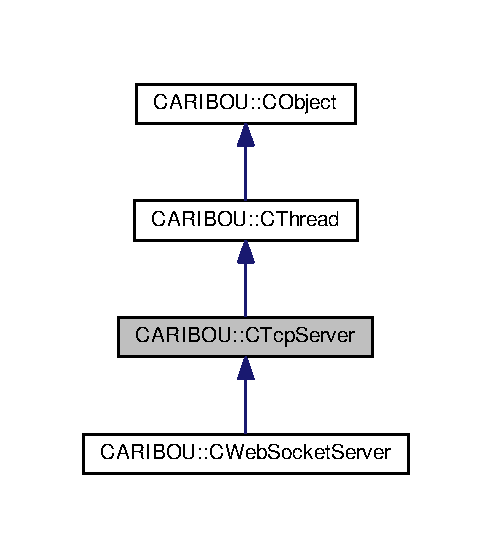
\includegraphics[width=236pt]{class_c_a_r_i_b_o_u_1_1_c_tcp_server__inherit__graph}
\end{center}
\end{figure}


Collaboration diagram for C\+A\+R\+I\+B\+OU\+:\+:C\+Tcp\+Server\+:\nopagebreak
\begin{figure}[H]
\begin{center}
\leavevmode
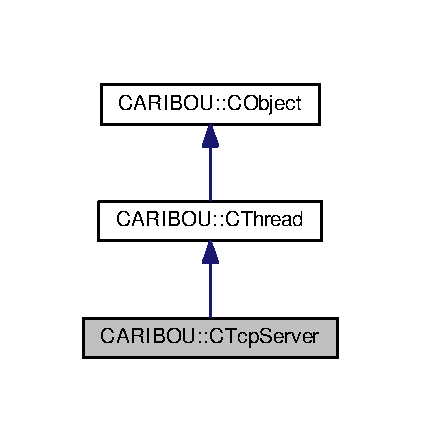
\includegraphics[width=202pt]{class_c_a_r_i_b_o_u_1_1_c_tcp_server__coll__graph}
\end{center}
\end{figure}
\subsection*{Public Member Functions}
\begin{DoxyCompactItemize}
\item 
{\bf C\+Tcp\+Server} (uint16\+\_\+t {\bf port}, uint32\+\_\+t {\bf interface}=I\+N\+A\+D\+D\+R\+\_\+\+A\+NY, int backlog=T\+C\+P\+\_\+\+D\+E\+F\+A\+U\+L\+T\+\_\+\+L\+I\+S\+T\+E\+N\+\_\+\+B\+A\+C\+K\+L\+OG, char $\ast${\bf name}=\char`\"{}tcpsrv\char`\"{}, uint32\+\_\+t stksize=512, uint16\+\_\+t {\bf priority}=0)
\begin{DoxyCompactList}\small\item\em A T\+CP server instance will set up a listener on the T\+CP port. \end{DoxyCompactList}\item 
virtual {\bf $\sim$\+C\+Tcp\+Server} ()
\item 
uint32\+\_\+t {\bf interface} ()
\item 
uint16\+\_\+t {\bf port} ()
\item 
bool {\bf is\+Valid} ()
\begin{DoxyCompactList}\small\item\em Determine if the server is valid. \end{DoxyCompactList}\item 
void {\bf close} ()
\item 
virtual void {\bf run} ()
\end{DoxyCompactItemize}
\subsection*{Static Public Member Functions}
\begin{DoxyCompactItemize}
\item 
static {\bf C\+List}$<$ {\bf C\+Tcp\+Server} $\ast$ $>$ \& {\bf servers} ()
\begin{DoxyCompactList}\small\item\em Return the list of servers. \end{DoxyCompactList}\item 
static {\bf C\+Tcp\+Server} $\ast$ {\bf server} (uint16\+\_\+t {\bf port})
\begin{DoxyCompactList}\small\item\em Locate the T\+CP server instance servicing the port. \end{DoxyCompactList}\end{DoxyCompactItemize}
\subsection*{Protected Member Functions}
\begin{DoxyCompactItemize}
\item 
virtual void {\bf accept\+Error} (int rc, int err, const char $\ast$msg={\bf N\+U\+LL})
\item 
virtual void {\bf listen\+Error} (int rc, int err, const char $\ast$msg={\bf N\+U\+LL})
\item 
virtual void {\bf bind\+Error} (int rc, int err, const char $\ast$msg={\bf N\+U\+LL})
\item 
virtual void {\bf socket\+Error} (int rc, int err, const char $\ast$msg={\bf N\+U\+LL})
\item 
bool {\bf increment\+Connections} ()
\item 
bool {\bf decrement\+Connections} ()
\item 
virtual bool {\bf fork} ({\bf C\+A\+R\+I\+B\+O\+U\+::\+C\+Abstract\+Socket} $\ast$socket)
\begin{DoxyCompactList}\small\item\em This method should be overridden by the protocol server. \end{DoxyCompactList}\item 
virtual void {\bf idle} ()
\end{DoxyCompactItemize}
\subsection*{Protected Attributes}
\begin{DoxyCompactItemize}
\item 
uint32\+\_\+t {\bf m\+Interface}
\item 
uint16\+\_\+t {\bf m\+Port}
\item 
int {\bf m\+Backlog}
\item 
int {\bf m\+Server\+Socket}
\end{DoxyCompactItemize}
\subsection*{Additional Inherited Members}


\subsection{Detailed Description}
The tcp server object. 

\begin{DoxyAuthor}{Author}
Mike Sharkey {\tt mike@pikeaero.\+com} 
\end{DoxyAuthor}


Definition at line 32 of file ctcpserver.\+h.



\subsection{Constructor \& Destructor Documentation}
\index{C\+A\+R\+I\+B\+O\+U\+::\+C\+Tcp\+Server@{C\+A\+R\+I\+B\+O\+U\+::\+C\+Tcp\+Server}!C\+Tcp\+Server@{C\+Tcp\+Server}}
\index{C\+Tcp\+Server@{C\+Tcp\+Server}!C\+A\+R\+I\+B\+O\+U\+::\+C\+Tcp\+Server@{C\+A\+R\+I\+B\+O\+U\+::\+C\+Tcp\+Server}}
\subsubsection[{C\+Tcp\+Server(uint16\+\_\+t port, uint32\+\_\+t interface=\+I\+N\+A\+D\+D\+R\+\_\+\+A\+N\+Y, int backlog=\+T\+C\+P\+\_\+\+D\+E\+F\+A\+U\+L\+T\+\_\+\+L\+I\+S\+T\+E\+N\+\_\+\+B\+A\+C\+K\+L\+O\+G, char $\ast$name=""tcpsrv"", uint32\+\_\+t stksize=512, uint16\+\_\+t priority=0)}]{\setlength{\rightskip}{0pt plus 5cm}C\+A\+R\+I\+B\+O\+U\+::\+C\+Tcp\+Server\+::\+C\+Tcp\+Server (
\begin{DoxyParamCaption}
\item[{uint16\+\_\+t}]{port, }
\item[{uint32\+\_\+t}]{interface = {\ttfamily INADDR\+\_\+ANY}, }
\item[{int}]{backlog = {\ttfamily TCP\+\_\+DEFAULT\+\_\+LISTEN\+\_\+BACKLOG}, }
\item[{char $\ast$}]{name = {\ttfamily \char`\"{}tcpsrv\char`\"{}}, }
\item[{uint32\+\_\+t}]{stksize = {\ttfamily 512}, }
\item[{uint16\+\_\+t}]{priority = {\ttfamily 0}}
\end{DoxyParamCaption}
)}\label{class_c_a_r_i_b_o_u_1_1_c_tcp_server_ad2014b134cae2da8a39f47c0030b3cf6}


A T\+CP server instance will set up a listener on the T\+CP port. 



Definition at line 27 of file ctcpserver.\+cpp.

\index{C\+A\+R\+I\+B\+O\+U\+::\+C\+Tcp\+Server@{C\+A\+R\+I\+B\+O\+U\+::\+C\+Tcp\+Server}!````~C\+Tcp\+Server@{$\sim$\+C\+Tcp\+Server}}
\index{````~C\+Tcp\+Server@{$\sim$\+C\+Tcp\+Server}!C\+A\+R\+I\+B\+O\+U\+::\+C\+Tcp\+Server@{C\+A\+R\+I\+B\+O\+U\+::\+C\+Tcp\+Server}}
\subsubsection[{$\sim$\+C\+Tcp\+Server()}]{\setlength{\rightskip}{0pt plus 5cm}C\+A\+R\+I\+B\+O\+U\+::\+C\+Tcp\+Server\+::$\sim$\+C\+Tcp\+Server (
\begin{DoxyParamCaption}
{}
\end{DoxyParamCaption}
)\hspace{0.3cm}{\ttfamily [virtual]}}\label{class_c_a_r_i_b_o_u_1_1_c_tcp_server_aa7ee902ec41feda915dd582682f135d7}


Definition at line 39 of file ctcpserver.\+cpp.



\subsection{Member Function Documentation}
\index{C\+A\+R\+I\+B\+O\+U\+::\+C\+Tcp\+Server@{C\+A\+R\+I\+B\+O\+U\+::\+C\+Tcp\+Server}!accept\+Error@{accept\+Error}}
\index{accept\+Error@{accept\+Error}!C\+A\+R\+I\+B\+O\+U\+::\+C\+Tcp\+Server@{C\+A\+R\+I\+B\+O\+U\+::\+C\+Tcp\+Server}}
\subsubsection[{accept\+Error(int rc, int err, const char $\ast$msg=\+N\+U\+L\+L)}]{\setlength{\rightskip}{0pt plus 5cm}virtual void C\+A\+R\+I\+B\+O\+U\+::\+C\+Tcp\+Server\+::accept\+Error (
\begin{DoxyParamCaption}
\item[{int}]{rc, }
\item[{int}]{err, }
\item[{const char $\ast$}]{msg = {\ttfamily {\bf N\+U\+LL}}}
\end{DoxyParamCaption}
)\hspace{0.3cm}{\ttfamily [inline]}, {\ttfamily [protected]}, {\ttfamily [virtual]}}\label{class_c_a_r_i_b_o_u_1_1_c_tcp_server_a458a56a9dd350a3e3e7af57333857dd3}


Definition at line 48 of file ctcpserver.\+h.

\index{C\+A\+R\+I\+B\+O\+U\+::\+C\+Tcp\+Server@{C\+A\+R\+I\+B\+O\+U\+::\+C\+Tcp\+Server}!bind\+Error@{bind\+Error}}
\index{bind\+Error@{bind\+Error}!C\+A\+R\+I\+B\+O\+U\+::\+C\+Tcp\+Server@{C\+A\+R\+I\+B\+O\+U\+::\+C\+Tcp\+Server}}
\subsubsection[{bind\+Error(int rc, int err, const char $\ast$msg=\+N\+U\+L\+L)}]{\setlength{\rightskip}{0pt plus 5cm}virtual void C\+A\+R\+I\+B\+O\+U\+::\+C\+Tcp\+Server\+::bind\+Error (
\begin{DoxyParamCaption}
\item[{int}]{rc, }
\item[{int}]{err, }
\item[{const char $\ast$}]{msg = {\ttfamily {\bf N\+U\+LL}}}
\end{DoxyParamCaption}
)\hspace{0.3cm}{\ttfamily [inline]}, {\ttfamily [protected]}, {\ttfamily [virtual]}}\label{class_c_a_r_i_b_o_u_1_1_c_tcp_server_a45d1331e57caa785a8b9ee6cde1008ca}


Definition at line 50 of file ctcpserver.\+h.

\index{C\+A\+R\+I\+B\+O\+U\+::\+C\+Tcp\+Server@{C\+A\+R\+I\+B\+O\+U\+::\+C\+Tcp\+Server}!close@{close}}
\index{close@{close}!C\+A\+R\+I\+B\+O\+U\+::\+C\+Tcp\+Server@{C\+A\+R\+I\+B\+O\+U\+::\+C\+Tcp\+Server}}
\subsubsection[{close()}]{\setlength{\rightskip}{0pt plus 5cm}void C\+A\+R\+I\+B\+O\+U\+::\+C\+Tcp\+Server\+::close (
\begin{DoxyParamCaption}
{}
\end{DoxyParamCaption}
)}\label{class_c_a_r_i_b_o_u_1_1_c_tcp_server_a1724413b09111ce8dcb086ae20da631f}


Definition at line 58 of file ctcpserver.\+cpp.

\index{C\+A\+R\+I\+B\+O\+U\+::\+C\+Tcp\+Server@{C\+A\+R\+I\+B\+O\+U\+::\+C\+Tcp\+Server}!decrement\+Connections@{decrement\+Connections}}
\index{decrement\+Connections@{decrement\+Connections}!C\+A\+R\+I\+B\+O\+U\+::\+C\+Tcp\+Server@{C\+A\+R\+I\+B\+O\+U\+::\+C\+Tcp\+Server}}
\subsubsection[{decrement\+Connections()}]{\setlength{\rightskip}{0pt plus 5cm}bool C\+A\+R\+I\+B\+O\+U\+::\+C\+Tcp\+Server\+::decrement\+Connections (
\begin{DoxyParamCaption}
{}
\end{DoxyParamCaption}
)\hspace{0.3cm}{\ttfamily [protected]}}\label{class_c_a_r_i_b_o_u_1_1_c_tcp_server_ade37a3b8a0a4a550004dc952aaf918ff}
\index{C\+A\+R\+I\+B\+O\+U\+::\+C\+Tcp\+Server@{C\+A\+R\+I\+B\+O\+U\+::\+C\+Tcp\+Server}!fork@{fork}}
\index{fork@{fork}!C\+A\+R\+I\+B\+O\+U\+::\+C\+Tcp\+Server@{C\+A\+R\+I\+B\+O\+U\+::\+C\+Tcp\+Server}}
\subsubsection[{fork(\+C\+A\+R\+I\+B\+O\+U\+::\+C\+Abstract\+Socket $\ast$socket)}]{\setlength{\rightskip}{0pt plus 5cm}bool C\+A\+R\+I\+B\+O\+U\+::\+C\+Tcp\+Server\+::fork (
\begin{DoxyParamCaption}
\item[{{\bf C\+A\+R\+I\+B\+O\+U\+::\+C\+Abstract\+Socket} $\ast$}]{socket}
\end{DoxyParamCaption}
)\hspace{0.3cm}{\ttfamily [protected]}, {\ttfamily [virtual]}}\label{class_c_a_r_i_b_o_u_1_1_c_tcp_server_a8fada95aec44046c7f7b5b23833af9ce}


This method should be overridden by the protocol server. 

Fork a Web\+Sockets session...

The default implementation instantiates A C\+T\+C\+P\+Session base class (echo session) 

Definition at line 115 of file ctcpserver.\+cpp.

\index{C\+A\+R\+I\+B\+O\+U\+::\+C\+Tcp\+Server@{C\+A\+R\+I\+B\+O\+U\+::\+C\+Tcp\+Server}!idle@{idle}}
\index{idle@{idle}!C\+A\+R\+I\+B\+O\+U\+::\+C\+Tcp\+Server@{C\+A\+R\+I\+B\+O\+U\+::\+C\+Tcp\+Server}}
\subsubsection[{idle()}]{\setlength{\rightskip}{0pt plus 5cm}virtual void C\+A\+R\+I\+B\+O\+U\+::\+C\+Tcp\+Server\+::idle (
\begin{DoxyParamCaption}
{}
\end{DoxyParamCaption}
)\hspace{0.3cm}{\ttfamily [inline]}, {\ttfamily [protected]}, {\ttfamily [virtual]}}\label{class_c_a_r_i_b_o_u_1_1_c_tcp_server_a835e384f51f1b30c88716970f0226225}


Definition at line 56 of file ctcpserver.\+h.

\index{C\+A\+R\+I\+B\+O\+U\+::\+C\+Tcp\+Server@{C\+A\+R\+I\+B\+O\+U\+::\+C\+Tcp\+Server}!increment\+Connections@{increment\+Connections}}
\index{increment\+Connections@{increment\+Connections}!C\+A\+R\+I\+B\+O\+U\+::\+C\+Tcp\+Server@{C\+A\+R\+I\+B\+O\+U\+::\+C\+Tcp\+Server}}
\subsubsection[{increment\+Connections()}]{\setlength{\rightskip}{0pt plus 5cm}bool C\+A\+R\+I\+B\+O\+U\+::\+C\+Tcp\+Server\+::increment\+Connections (
\begin{DoxyParamCaption}
{}
\end{DoxyParamCaption}
)\hspace{0.3cm}{\ttfamily [protected]}}\label{class_c_a_r_i_b_o_u_1_1_c_tcp_server_a8571de40d930962cbb2a79bd90219c64}
\index{C\+A\+R\+I\+B\+O\+U\+::\+C\+Tcp\+Server@{C\+A\+R\+I\+B\+O\+U\+::\+C\+Tcp\+Server}!interface@{interface}}
\index{interface@{interface}!C\+A\+R\+I\+B\+O\+U\+::\+C\+Tcp\+Server@{C\+A\+R\+I\+B\+O\+U\+::\+C\+Tcp\+Server}}
\subsubsection[{interface()}]{\setlength{\rightskip}{0pt plus 5cm}uint32\+\_\+t C\+A\+R\+I\+B\+O\+U\+::\+C\+Tcp\+Server\+::interface (
\begin{DoxyParamCaption}
{}
\end{DoxyParamCaption}
)}\label{class_c_a_r_i_b_o_u_1_1_c_tcp_server_afac755ffe567f606e6591bd3024e06ad}
\begin{DoxyReturn}{Returns}
The address of the interface 
\end{DoxyReturn}


Definition at line 90 of file ctcpserver.\+cpp.

\index{C\+A\+R\+I\+B\+O\+U\+::\+C\+Tcp\+Server@{C\+A\+R\+I\+B\+O\+U\+::\+C\+Tcp\+Server}!is\+Valid@{is\+Valid}}
\index{is\+Valid@{is\+Valid}!C\+A\+R\+I\+B\+O\+U\+::\+C\+Tcp\+Server@{C\+A\+R\+I\+B\+O\+U\+::\+C\+Tcp\+Server}}
\subsubsection[{is\+Valid()}]{\setlength{\rightskip}{0pt plus 5cm}bool C\+A\+R\+I\+B\+O\+U\+::\+C\+Tcp\+Server\+::is\+Valid (
\begin{DoxyParamCaption}
{}
\end{DoxyParamCaption}
)}\label{class_c_a_r_i_b_o_u_1_1_c_tcp_server_ac16bbc71eb0d6a845fde93f5a8cd85c8}


Determine if the server is valid. 



Definition at line 53 of file ctcpserver.\+cpp.

\index{C\+A\+R\+I\+B\+O\+U\+::\+C\+Tcp\+Server@{C\+A\+R\+I\+B\+O\+U\+::\+C\+Tcp\+Server}!listen\+Error@{listen\+Error}}
\index{listen\+Error@{listen\+Error}!C\+A\+R\+I\+B\+O\+U\+::\+C\+Tcp\+Server@{C\+A\+R\+I\+B\+O\+U\+::\+C\+Tcp\+Server}}
\subsubsection[{listen\+Error(int rc, int err, const char $\ast$msg=\+N\+U\+L\+L)}]{\setlength{\rightskip}{0pt plus 5cm}virtual void C\+A\+R\+I\+B\+O\+U\+::\+C\+Tcp\+Server\+::listen\+Error (
\begin{DoxyParamCaption}
\item[{int}]{rc, }
\item[{int}]{err, }
\item[{const char $\ast$}]{msg = {\ttfamily {\bf N\+U\+LL}}}
\end{DoxyParamCaption}
)\hspace{0.3cm}{\ttfamily [inline]}, {\ttfamily [protected]}, {\ttfamily [virtual]}}\label{class_c_a_r_i_b_o_u_1_1_c_tcp_server_aad13c66b4749eadb213ac98d03c64fcb}


Definition at line 49 of file ctcpserver.\+h.

\index{C\+A\+R\+I\+B\+O\+U\+::\+C\+Tcp\+Server@{C\+A\+R\+I\+B\+O\+U\+::\+C\+Tcp\+Server}!port@{port}}
\index{port@{port}!C\+A\+R\+I\+B\+O\+U\+::\+C\+Tcp\+Server@{C\+A\+R\+I\+B\+O\+U\+::\+C\+Tcp\+Server}}
\subsubsection[{port()}]{\setlength{\rightskip}{0pt plus 5cm}uint16\+\_\+t C\+A\+R\+I\+B\+O\+U\+::\+C\+Tcp\+Server\+::port (
\begin{DoxyParamCaption}
{}
\end{DoxyParamCaption}
)}\label{class_c_a_r_i_b_o_u_1_1_c_tcp_server_addbdb44aad437fa86ba8744f208b574f}
\begin{DoxyReturn}{Returns}
The port of the interface 
\end{DoxyReturn}


Definition at line 106 of file ctcpserver.\+cpp.

\index{C\+A\+R\+I\+B\+O\+U\+::\+C\+Tcp\+Server@{C\+A\+R\+I\+B\+O\+U\+::\+C\+Tcp\+Server}!run@{run}}
\index{run@{run}!C\+A\+R\+I\+B\+O\+U\+::\+C\+Tcp\+Server@{C\+A\+R\+I\+B\+O\+U\+::\+C\+Tcp\+Server}}
\subsubsection[{run()}]{\setlength{\rightskip}{0pt plus 5cm}void C\+A\+R\+I\+B\+O\+U\+::\+C\+Tcp\+Server\+::run (
\begin{DoxyParamCaption}
{}
\end{DoxyParamCaption}
)\hspace{0.3cm}{\ttfamily [virtual]}}\label{class_c_a_r_i_b_o_u_1_1_c_tcp_server_a4d38415ea32f02035266cb34433ff392}


Implements {\bf C\+A\+R\+I\+B\+O\+U\+::\+C\+Thread} \doxyref{}{p.}{class_c_a_r_i_b_o_u_1_1_c_thread_a087ae48a158aca84892aea7f9ed16711}.



Reimplemented in {\bf C\+A\+R\+I\+B\+O\+U\+::\+C\+Web\+Socket\+Server} \doxyref{}{p.}{class_c_a_r_i_b_o_u_1_1_c_web_socket_server_a92d612844ad0295da21ebd0834ad5dc2}.



Definition at line 130 of file ctcpserver.\+cpp.

\index{C\+A\+R\+I\+B\+O\+U\+::\+C\+Tcp\+Server@{C\+A\+R\+I\+B\+O\+U\+::\+C\+Tcp\+Server}!server@{server}}
\index{server@{server}!C\+A\+R\+I\+B\+O\+U\+::\+C\+Tcp\+Server@{C\+A\+R\+I\+B\+O\+U\+::\+C\+Tcp\+Server}}
\subsubsection[{server(uint16\+\_\+t port)}]{\setlength{\rightskip}{0pt plus 5cm}{\bf C\+Tcp\+Server} $\ast$ C\+A\+R\+I\+B\+O\+U\+::\+C\+Tcp\+Server\+::server (
\begin{DoxyParamCaption}
\item[{uint16\+\_\+t}]{port}
\end{DoxyParamCaption}
)\hspace{0.3cm}{\ttfamily [static]}}\label{class_c_a_r_i_b_o_u_1_1_c_tcp_server_a1bd0115dbde216298e5ef78e54b5bb8f}


Locate the T\+CP server instance servicing the port. 


\begin{DoxyParams}{Parameters}
{\em port} & The port to search for. \\
\hline
\end{DoxyParams}
\begin{DoxyReturn}{Returns}
Return the server instance or N\+U\+LL. 
\end{DoxyReturn}


Definition at line 70 of file ctcpserver.\+cpp.

\index{C\+A\+R\+I\+B\+O\+U\+::\+C\+Tcp\+Server@{C\+A\+R\+I\+B\+O\+U\+::\+C\+Tcp\+Server}!servers@{servers}}
\index{servers@{servers}!C\+A\+R\+I\+B\+O\+U\+::\+C\+Tcp\+Server@{C\+A\+R\+I\+B\+O\+U\+::\+C\+Tcp\+Server}}
\subsubsection[{servers()}]{\setlength{\rightskip}{0pt plus 5cm}{\bf C\+List}$<$ {\bf C\+Tcp\+Server} $\ast$ $>$ \& C\+A\+R\+I\+B\+O\+U\+::\+C\+Tcp\+Server\+::servers (
\begin{DoxyParamCaption}
{}
\end{DoxyParamCaption}
)\hspace{0.3cm}{\ttfamily [static]}}\label{class_c_a_r_i_b_o_u_1_1_c_tcp_server_a829434bca875859c8adf30d5152f61c1}


Return the list of servers. 



Definition at line 47 of file ctcpserver.\+cpp.

\index{C\+A\+R\+I\+B\+O\+U\+::\+C\+Tcp\+Server@{C\+A\+R\+I\+B\+O\+U\+::\+C\+Tcp\+Server}!socket\+Error@{socket\+Error}}
\index{socket\+Error@{socket\+Error}!C\+A\+R\+I\+B\+O\+U\+::\+C\+Tcp\+Server@{C\+A\+R\+I\+B\+O\+U\+::\+C\+Tcp\+Server}}
\subsubsection[{socket\+Error(int rc, int err, const char $\ast$msg=\+N\+U\+L\+L)}]{\setlength{\rightskip}{0pt plus 5cm}virtual void C\+A\+R\+I\+B\+O\+U\+::\+C\+Tcp\+Server\+::socket\+Error (
\begin{DoxyParamCaption}
\item[{int}]{rc, }
\item[{int}]{err, }
\item[{const char $\ast$}]{msg = {\ttfamily {\bf N\+U\+LL}}}
\end{DoxyParamCaption}
)\hspace{0.3cm}{\ttfamily [inline]}, {\ttfamily [protected]}, {\ttfamily [virtual]}}\label{class_c_a_r_i_b_o_u_1_1_c_tcp_server_a4ca81c6ca563028fa4dbcfbbf7ffd807}


Definition at line 51 of file ctcpserver.\+h.



\subsection{Member Data Documentation}
\index{C\+A\+R\+I\+B\+O\+U\+::\+C\+Tcp\+Server@{C\+A\+R\+I\+B\+O\+U\+::\+C\+Tcp\+Server}!m\+Backlog@{m\+Backlog}}
\index{m\+Backlog@{m\+Backlog}!C\+A\+R\+I\+B\+O\+U\+::\+C\+Tcp\+Server@{C\+A\+R\+I\+B\+O\+U\+::\+C\+Tcp\+Server}}
\subsubsection[{m\+Backlog}]{\setlength{\rightskip}{0pt plus 5cm}int C\+A\+R\+I\+B\+O\+U\+::\+C\+Tcp\+Server\+::m\+Backlog\hspace{0.3cm}{\ttfamily [protected]}}\label{class_c_a_r_i_b_o_u_1_1_c_tcp_server_aa11e930abd845df192865178d6bc3e24}


Definition at line 60 of file ctcpserver.\+h.

\index{C\+A\+R\+I\+B\+O\+U\+::\+C\+Tcp\+Server@{C\+A\+R\+I\+B\+O\+U\+::\+C\+Tcp\+Server}!m\+Interface@{m\+Interface}}
\index{m\+Interface@{m\+Interface}!C\+A\+R\+I\+B\+O\+U\+::\+C\+Tcp\+Server@{C\+A\+R\+I\+B\+O\+U\+::\+C\+Tcp\+Server}}
\subsubsection[{m\+Interface}]{\setlength{\rightskip}{0pt plus 5cm}uint32\+\_\+t C\+A\+R\+I\+B\+O\+U\+::\+C\+Tcp\+Server\+::m\+Interface\hspace{0.3cm}{\ttfamily [protected]}}\label{class_c_a_r_i_b_o_u_1_1_c_tcp_server_a71b081507b8187da8f7d58774cc19647}


Definition at line 56 of file ctcpserver.\+h.

\index{C\+A\+R\+I\+B\+O\+U\+::\+C\+Tcp\+Server@{C\+A\+R\+I\+B\+O\+U\+::\+C\+Tcp\+Server}!m\+Port@{m\+Port}}
\index{m\+Port@{m\+Port}!C\+A\+R\+I\+B\+O\+U\+::\+C\+Tcp\+Server@{C\+A\+R\+I\+B\+O\+U\+::\+C\+Tcp\+Server}}
\subsubsection[{m\+Port}]{\setlength{\rightskip}{0pt plus 5cm}uint16\+\_\+t C\+A\+R\+I\+B\+O\+U\+::\+C\+Tcp\+Server\+::m\+Port\hspace{0.3cm}{\ttfamily [protected]}}\label{class_c_a_r_i_b_o_u_1_1_c_tcp_server_a0040a0bd02f6c68f53adbd8bd3286944}


Definition at line 59 of file ctcpserver.\+h.

\index{C\+A\+R\+I\+B\+O\+U\+::\+C\+Tcp\+Server@{C\+A\+R\+I\+B\+O\+U\+::\+C\+Tcp\+Server}!m\+Server\+Socket@{m\+Server\+Socket}}
\index{m\+Server\+Socket@{m\+Server\+Socket}!C\+A\+R\+I\+B\+O\+U\+::\+C\+Tcp\+Server@{C\+A\+R\+I\+B\+O\+U\+::\+C\+Tcp\+Server}}
\subsubsection[{m\+Server\+Socket}]{\setlength{\rightskip}{0pt plus 5cm}int C\+A\+R\+I\+B\+O\+U\+::\+C\+Tcp\+Server\+::m\+Server\+Socket\hspace{0.3cm}{\ttfamily [protected]}}\label{class_c_a_r_i_b_o_u_1_1_c_tcp_server_a52f5315f9f4362c416bda79da096a811}


Definition at line 61 of file ctcpserver.\+h.



The documentation for this class was generated from the following files\+:\begin{DoxyCompactItemize}
\item 
include/caribou++/{\bf ctcpserver.\+h}\item 
src/{\bf ctcpserver.\+cpp}\item 
src/{\bf cwebsocketserver.\+cpp}\end{DoxyCompactItemize}

\section{C\-A\-R\-I\-B\-O\-U\-:\-:C\-Tcp\-Session Class Reference}
\label{class_c_a_r_i_b_o_u_1_1_c_tcp_session}\index{C\-A\-R\-I\-B\-O\-U\-::\-C\-Tcp\-Session@{C\-A\-R\-I\-B\-O\-U\-::\-C\-Tcp\-Session}}


{\ttfamily \#include $<$ctcpsession.\-h$>$}



Inheritance diagram for C\-A\-R\-I\-B\-O\-U\-:\-:C\-Tcp\-Session\-:\nopagebreak
\begin{figure}[H]
\begin{center}
\leavevmode
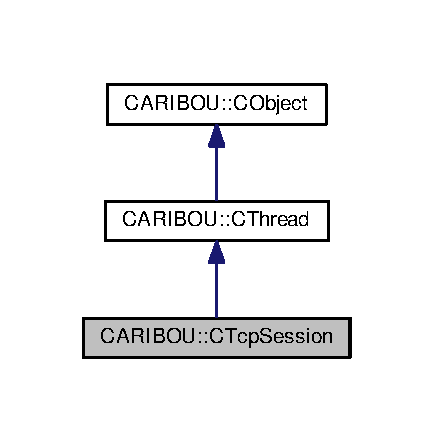
\includegraphics[width=208pt]{class_c_a_r_i_b_o_u_1_1_c_tcp_session__inherit__graph}
\end{center}
\end{figure}


Collaboration diagram for C\-A\-R\-I\-B\-O\-U\-:\-:C\-Tcp\-Session\-:\nopagebreak
\begin{figure}[H]
\begin{center}
\leavevmode
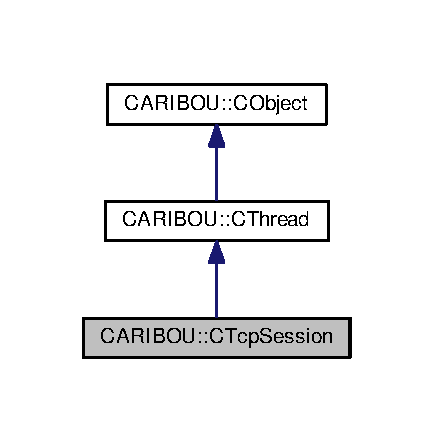
\includegraphics[width=208pt]{class_c_a_r_i_b_o_u_1_1_c_tcp_session__coll__graph}
\end{center}
\end{figure}
\subsection*{Public Member Functions}
\begin{DoxyCompactItemize}
\item 
{\bf C\-Tcp\-Session} (int socket, const char $\ast${\bf name}=\char`\"{}tcp\char`\"{}, uint16\-\_\-t stksize=1024, uint16\-\_\-t {\bf priority}=1)
\item 
virtual {\bf $\sim$\-C\-Tcp\-Session} ()
\end{DoxyCompactItemize}
\subsection*{Protected Member Functions}
\begin{DoxyCompactItemize}
\item 
virtual void {\bf run} ()
\begin{DoxyCompactList}\small\item\em This method should be overridden by the T\-C\-P protocol server. \end{DoxyCompactList}\end{DoxyCompactItemize}
\subsection*{Additional Inherited Members}


\subsection{Detailed Description}


Definition at line 24 of file ctcpsession.\-h.



\subsection{Constructor \& Destructor Documentation}
\index{C\-A\-R\-I\-B\-O\-U\-::\-C\-Tcp\-Session@{C\-A\-R\-I\-B\-O\-U\-::\-C\-Tcp\-Session}!C\-Tcp\-Session@{C\-Tcp\-Session}}
\index{C\-Tcp\-Session@{C\-Tcp\-Session}!CARIBOU::CTcpSession@{C\-A\-R\-I\-B\-O\-U\-::\-C\-Tcp\-Session}}
\subsubsection[{C\-Tcp\-Session}]{\setlength{\rightskip}{0pt plus 5cm}C\-A\-R\-I\-B\-O\-U\-::\-C\-Tcp\-Session\-::\-C\-Tcp\-Session (
\begin{DoxyParamCaption}
\item[{int}]{socket, }
\item[{const char $\ast$}]{name = {\ttfamily \char`\"{}tcp\char`\"{}}, }
\item[{uint16\-\_\-t}]{stksize = {\ttfamily 1024}, }
\item[{uint16\-\_\-t}]{priority = {\ttfamily 1}}
\end{DoxyParamCaption}
)}\label{class_c_a_r_i_b_o_u_1_1_c_tcp_session_add22726f810e0337cdf5d3b771716c23}


Definition at line 22 of file ctcpsession.\-cpp.

\index{C\-A\-R\-I\-B\-O\-U\-::\-C\-Tcp\-Session@{C\-A\-R\-I\-B\-O\-U\-::\-C\-Tcp\-Session}!$\sim$\-C\-Tcp\-Session@{$\sim$\-C\-Tcp\-Session}}
\index{$\sim$\-C\-Tcp\-Session@{$\sim$\-C\-Tcp\-Session}!CARIBOU::CTcpSession@{C\-A\-R\-I\-B\-O\-U\-::\-C\-Tcp\-Session}}
\subsubsection[{$\sim$\-C\-Tcp\-Session}]{\setlength{\rightskip}{0pt plus 5cm}C\-A\-R\-I\-B\-O\-U\-::\-C\-Tcp\-Session\-::$\sim$\-C\-Tcp\-Session (
\begin{DoxyParamCaption}
{}
\end{DoxyParamCaption}
)\hspace{0.3cm}{\ttfamily [virtual]}}\label{class_c_a_r_i_b_o_u_1_1_c_tcp_session_a0046e4c0300258f82716c6c6d21465af}


Definition at line 28 of file ctcpsession.\-cpp.



\subsection{Member Function Documentation}
\index{C\-A\-R\-I\-B\-O\-U\-::\-C\-Tcp\-Session@{C\-A\-R\-I\-B\-O\-U\-::\-C\-Tcp\-Session}!run@{run}}
\index{run@{run}!CARIBOU::CTcpSession@{C\-A\-R\-I\-B\-O\-U\-::\-C\-Tcp\-Session}}
\subsubsection[{run}]{\setlength{\rightskip}{0pt plus 5cm}void C\-A\-R\-I\-B\-O\-U\-::\-C\-Tcp\-Session\-::run (
\begin{DoxyParamCaption}
{}
\end{DoxyParamCaption}
)\hspace{0.3cm}{\ttfamily [protected]}, {\ttfamily [virtual]}}\label{class_c_a_r_i_b_o_u_1_1_c_tcp_session_a66d1ace1fb86d1f41c587aff037adc12}


This method should be overridden by the T\-C\-P protocol server. 

The default implementation is a simple echo server.... 

Implements {\bf C\-A\-R\-I\-B\-O\-U\-::\-C\-Thread} \doxyref{}{p.}{class_c_a_r_i_b_o_u_1_1_c_thread_a087ae48a158aca84892aea7f9ed16711}.



Definition at line 42 of file ctcpsession.\-cpp.



The documentation for this class was generated from the following files\-:\begin{DoxyCompactItemize}
\item 
include/caribou++/{\bf ctcpsession.\-h}\item 
src/{\bf ctcpsession.\-cpp}\end{DoxyCompactItemize}

\section{C\-A\-R\-I\-B\-O\-U\-:\-:C\-Tcp\-Socket Class Reference}
\label{class_c_a_r_i_b_o_u_1_1_c_tcp_socket}\index{C\-A\-R\-I\-B\-O\-U\-::\-C\-Tcp\-Socket@{C\-A\-R\-I\-B\-O\-U\-::\-C\-Tcp\-Socket}}


The \doxyref{C\-Tcp\-Socket}{p.}{class_c_a_r_i_b_o_u_1_1_c_tcp_socket} class provides a T\-C\-P socket.  




{\ttfamily \#include $<$ctcpsocket.\-h$>$}



Inheritance diagram for C\-A\-R\-I\-B\-O\-U\-:\-:C\-Tcp\-Socket\-:\nopagebreak
\begin{figure}[H]
\begin{center}
\leavevmode
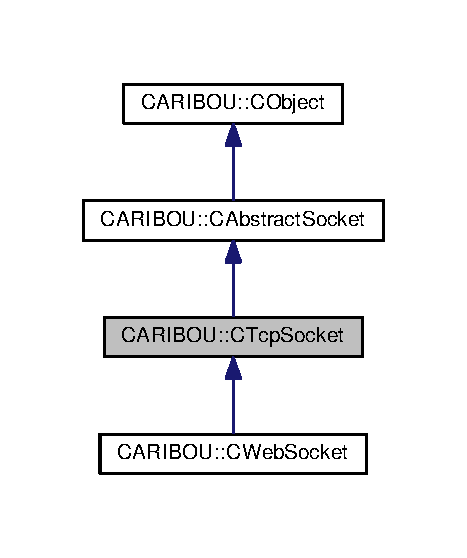
\includegraphics[width=224pt]{class_c_a_r_i_b_o_u_1_1_c_tcp_socket__inherit__graph}
\end{center}
\end{figure}


Collaboration diagram for C\-A\-R\-I\-B\-O\-U\-:\-:C\-Tcp\-Socket\-:\nopagebreak
\begin{figure}[H]
\begin{center}
\leavevmode
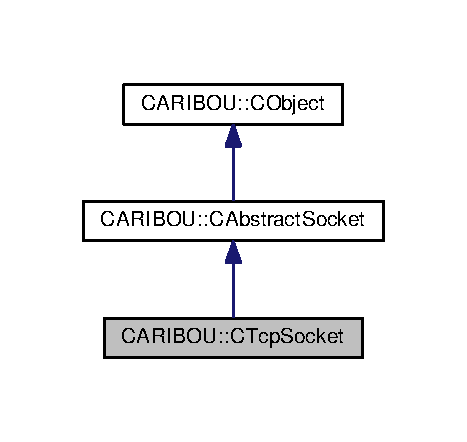
\includegraphics[width=224pt]{class_c_a_r_i_b_o_u_1_1_c_tcp_socket__coll__graph}
\end{center}
\end{figure}
\subsection*{Public Member Functions}
\begin{DoxyCompactItemize}
\item 
{\bf C\-Tcp\-Socket} ()
\item 
{\bf C\-Tcp\-Socket} (int {\bf socket})
\item 
{\bf C\-Tcp\-Socket} (int domain, int type, int protocol)
\item 
{\bf C\-Tcp\-Socket} (const {\bf C\-Tcp\-Socket} \&other)
\item 
virtual {\bf $\sim$\-C\-Tcp\-Socket} ()
\item 
{\bf C\-Tcp\-Socket} \& {\bf operator=} (const {\bf C\-Tcp\-Socket} \&other)
\item 
bool {\bf operator==} ({\bf C\-Tcp\-Socket} \&other)
\end{DoxyCompactItemize}
\subsection*{Additional Inherited Members}


\subsection{Detailed Description}
The \doxyref{C\-Tcp\-Socket}{p.}{class_c_a_r_i_b_o_u_1_1_c_tcp_socket} class provides a T\-C\-P socket. 

T\-C\-P (Transmission Control Protocol) is a reliable, stream-\/oriented, connection-\/oriented transport protocol. It is especially well suited for continuous transmission of data. 

Definition at line 29 of file ctcpsocket.\-h.



\subsection{Constructor \& Destructor Documentation}
\index{C\-A\-R\-I\-B\-O\-U\-::\-C\-Tcp\-Socket@{C\-A\-R\-I\-B\-O\-U\-::\-C\-Tcp\-Socket}!C\-Tcp\-Socket@{C\-Tcp\-Socket}}
\index{C\-Tcp\-Socket@{C\-Tcp\-Socket}!CARIBOU::CTcpSocket@{C\-A\-R\-I\-B\-O\-U\-::\-C\-Tcp\-Socket}}
\subsubsection[{C\-Tcp\-Socket}]{\setlength{\rightskip}{0pt plus 5cm}C\-A\-R\-I\-B\-O\-U\-::\-C\-Tcp\-Socket\-::\-C\-Tcp\-Socket (
\begin{DoxyParamCaption}
{}
\end{DoxyParamCaption}
)}\label{class_c_a_r_i_b_o_u_1_1_c_tcp_socket_abfcb4e33d5473696a7203e974c6b07f8}


Definition at line 21 of file ctcpsocket.\-cpp.

\index{C\-A\-R\-I\-B\-O\-U\-::\-C\-Tcp\-Socket@{C\-A\-R\-I\-B\-O\-U\-::\-C\-Tcp\-Socket}!C\-Tcp\-Socket@{C\-Tcp\-Socket}}
\index{C\-Tcp\-Socket@{C\-Tcp\-Socket}!CARIBOU::CTcpSocket@{C\-A\-R\-I\-B\-O\-U\-::\-C\-Tcp\-Socket}}
\subsubsection[{C\-Tcp\-Socket}]{\setlength{\rightskip}{0pt plus 5cm}C\-A\-R\-I\-B\-O\-U\-::\-C\-Tcp\-Socket\-::\-C\-Tcp\-Socket (
\begin{DoxyParamCaption}
\item[{int}]{socket}
\end{DoxyParamCaption}
)}\label{class_c_a_r_i_b_o_u_1_1_c_tcp_socket_a94832cf1d4a88da96022f1b5347f43ed}


Definition at line 26 of file ctcpsocket.\-cpp.

\index{C\-A\-R\-I\-B\-O\-U\-::\-C\-Tcp\-Socket@{C\-A\-R\-I\-B\-O\-U\-::\-C\-Tcp\-Socket}!C\-Tcp\-Socket@{C\-Tcp\-Socket}}
\index{C\-Tcp\-Socket@{C\-Tcp\-Socket}!CARIBOU::CTcpSocket@{C\-A\-R\-I\-B\-O\-U\-::\-C\-Tcp\-Socket}}
\subsubsection[{C\-Tcp\-Socket}]{\setlength{\rightskip}{0pt plus 5cm}C\-A\-R\-I\-B\-O\-U\-::\-C\-Tcp\-Socket\-::\-C\-Tcp\-Socket (
\begin{DoxyParamCaption}
\item[{int}]{domain, }
\item[{int}]{type, }
\item[{int}]{protocol}
\end{DoxyParamCaption}
)}\label{class_c_a_r_i_b_o_u_1_1_c_tcp_socket_a0716217863b33046e2260613fa6e1fdc}


Definition at line 31 of file ctcpsocket.\-cpp.

\index{C\-A\-R\-I\-B\-O\-U\-::\-C\-Tcp\-Socket@{C\-A\-R\-I\-B\-O\-U\-::\-C\-Tcp\-Socket}!C\-Tcp\-Socket@{C\-Tcp\-Socket}}
\index{C\-Tcp\-Socket@{C\-Tcp\-Socket}!CARIBOU::CTcpSocket@{C\-A\-R\-I\-B\-O\-U\-::\-C\-Tcp\-Socket}}
\subsubsection[{C\-Tcp\-Socket}]{\setlength{\rightskip}{0pt plus 5cm}C\-A\-R\-I\-B\-O\-U\-::\-C\-Tcp\-Socket\-::\-C\-Tcp\-Socket (
\begin{DoxyParamCaption}
\item[{const {\bf C\-Tcp\-Socket} \&}]{other}
\end{DoxyParamCaption}
)}\label{class_c_a_r_i_b_o_u_1_1_c_tcp_socket_a1bfdc259290c0077845f24b1b3296b1c}


Definition at line 36 of file ctcpsocket.\-cpp.

\index{C\-A\-R\-I\-B\-O\-U\-::\-C\-Tcp\-Socket@{C\-A\-R\-I\-B\-O\-U\-::\-C\-Tcp\-Socket}!$\sim$\-C\-Tcp\-Socket@{$\sim$\-C\-Tcp\-Socket}}
\index{$\sim$\-C\-Tcp\-Socket@{$\sim$\-C\-Tcp\-Socket}!CARIBOU::CTcpSocket@{C\-A\-R\-I\-B\-O\-U\-::\-C\-Tcp\-Socket}}
\subsubsection[{$\sim$\-C\-Tcp\-Socket}]{\setlength{\rightskip}{0pt plus 5cm}C\-A\-R\-I\-B\-O\-U\-::\-C\-Tcp\-Socket\-::$\sim$\-C\-Tcp\-Socket (
\begin{DoxyParamCaption}
{}
\end{DoxyParamCaption}
)\hspace{0.3cm}{\ttfamily [virtual]}}\label{class_c_a_r_i_b_o_u_1_1_c_tcp_socket_a5bb9cb1fcb1b1e74c711928eba5c9a83}


Definition at line 41 of file ctcpsocket.\-cpp.



\subsection{Member Function Documentation}
\index{C\-A\-R\-I\-B\-O\-U\-::\-C\-Tcp\-Socket@{C\-A\-R\-I\-B\-O\-U\-::\-C\-Tcp\-Socket}!operator=@{operator=}}
\index{operator=@{operator=}!CARIBOU::CTcpSocket@{C\-A\-R\-I\-B\-O\-U\-::\-C\-Tcp\-Socket}}
\subsubsection[{operator=}]{\setlength{\rightskip}{0pt plus 5cm}{\bf C\-Tcp\-Socket} \& C\-A\-R\-I\-B\-O\-U\-::\-C\-Tcp\-Socket\-::operator= (
\begin{DoxyParamCaption}
\item[{const {\bf C\-Tcp\-Socket} \&}]{other}
\end{DoxyParamCaption}
)}\label{class_c_a_r_i_b_o_u_1_1_c_tcp_socket_aa925693cc71430a592795749d23ae34b}


Definition at line 45 of file ctcpsocket.\-cpp.

\index{C\-A\-R\-I\-B\-O\-U\-::\-C\-Tcp\-Socket@{C\-A\-R\-I\-B\-O\-U\-::\-C\-Tcp\-Socket}!operator==@{operator==}}
\index{operator==@{operator==}!CARIBOU::CTcpSocket@{C\-A\-R\-I\-B\-O\-U\-::\-C\-Tcp\-Socket}}
\subsubsection[{operator==}]{\setlength{\rightskip}{0pt plus 5cm}bool C\-A\-R\-I\-B\-O\-U\-::\-C\-Tcp\-Socket\-::operator== (
\begin{DoxyParamCaption}
\item[{{\bf C\-Tcp\-Socket} \&}]{other}
\end{DoxyParamCaption}
)}\label{class_c_a_r_i_b_o_u_1_1_c_tcp_socket_a52fc7160cfeca70588533594703df470}


Definition at line 50 of file ctcpsocket.\-cpp.



The documentation for this class was generated from the following files\-:\begin{DoxyCompactItemize}
\item 
include/caribou++/{\bf ctcpsocket.\-h}\item 
src/{\bf ctcpsocket.\-cpp}\end{DoxyCompactItemize}

\section{C\-A\-R\-I\-B\-O\-U\-:\-:C\-Tcp\-Thread\-Event Class Reference}
\label{class_c_a_r_i_b_o_u_1_1_c_tcp_thread_event}\index{C\-A\-R\-I\-B\-O\-U\-::\-C\-Tcp\-Thread\-Event@{C\-A\-R\-I\-B\-O\-U\-::\-C\-Tcp\-Thread\-Event}}


{\ttfamily \#include $<$ctcpthreadevent.\-h$>$}



Inheritance diagram for C\-A\-R\-I\-B\-O\-U\-:\-:C\-Tcp\-Thread\-Event\-:\nopagebreak
\begin{figure}[H]
\begin{center}
\leavevmode
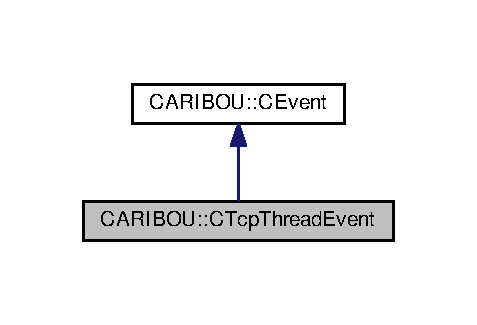
\includegraphics[width=228pt]{class_c_a_r_i_b_o_u_1_1_c_tcp_thread_event__inherit__graph}
\end{center}
\end{figure}


Collaboration diagram for C\-A\-R\-I\-B\-O\-U\-:\-:C\-Tcp\-Thread\-Event\-:\nopagebreak
\begin{figure}[H]
\begin{center}
\leavevmode
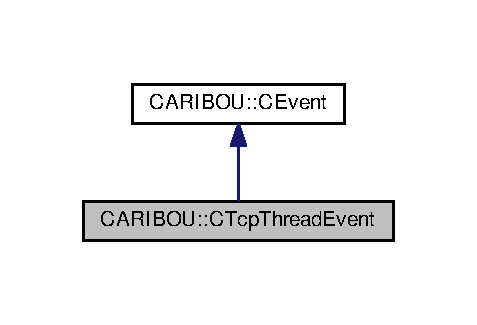
\includegraphics[width=228pt]{class_c_a_r_i_b_o_u_1_1_c_tcp_thread_event__coll__graph}
\end{center}
\end{figure}
\subsection*{Public Types}
\begin{DoxyCompactItemize}
\item 
enum {\bf tcp\-\_\-msg\-\_\-t} \{ \\*
{\bf msg\-None}, 
{\bf msg\-New}, 
{\bf msg\-Close}, 
{\bf msg\-Read}, 
\\*
{\bf msg\-Write}, 
{\bf msg\-Poll\-Read}, 
{\bf msg\-Poll\-Write}
 \}
\end{DoxyCompactItemize}
\subsection*{Public Member Functions}
\begin{DoxyCompactItemize}
\item 
{\bf C\-Tcp\-Thread\-Event} ({\bf C\-Object} $\ast${\bf sender})
\item 
{\bf C\-Tcp\-Thread\-Event} ({\bf C\-Tcp\-Thread\-Event} $\ast$other)
\item 
{\bf C\-Tcp\-Thread\-Event} ({\bf C\-Tcp\-Thread\-Event} \&other)
\item 
virtual {\bf $\sim$\-C\-Tcp\-Thread\-Event} ()
\item 
virtual void {\bf copy} ({\bf C\-Tcp\-Thread\-Event} \&other)
\item 
void {\bf set\-Socket} (int {\bf socket})
\item 
int {\bf socket} ()
\item 
void {\bf set\-Message} ({\bf tcp\-\_\-msg\-\_\-t} m)
\item 
{\bf tcp\-\_\-msg\-\_\-t} {\bf message} ()
\item 
void {\bf acknowledge} ()
\begin{DoxyCompactList}\small\item\em Tcp Server thread should acknowledge on startup (msg\-New) otherwise, socket will be closed. \end{DoxyCompactList}\end{DoxyCompactItemize}


\subsection{Detailed Description}


Definition at line 24 of file ctcpthreadevent.\-h.



\subsection{Member Enumeration Documentation}
\index{C\-A\-R\-I\-B\-O\-U\-::\-C\-Tcp\-Thread\-Event@{C\-A\-R\-I\-B\-O\-U\-::\-C\-Tcp\-Thread\-Event}!tcp\-\_\-msg\-\_\-t@{tcp\-\_\-msg\-\_\-t}}
\index{tcp\-\_\-msg\-\_\-t@{tcp\-\_\-msg\-\_\-t}!CARIBOU::CTcpThreadEvent@{C\-A\-R\-I\-B\-O\-U\-::\-C\-Tcp\-Thread\-Event}}
\subsubsection[{tcp\-\_\-msg\-\_\-t}]{\setlength{\rightskip}{0pt plus 5cm}enum {\bf C\-A\-R\-I\-B\-O\-U\-::\-C\-Tcp\-Thread\-Event\-::tcp\-\_\-msg\-\_\-t}}\label{class_c_a_r_i_b_o_u_1_1_c_tcp_thread_event_ab1b0a801936b492a8d8e3b5012e36676}
\begin{Desc}
\item[Enumerator]\par
\begin{description}
\index{msg\-None@{msg\-None}!C\-A\-R\-I\-B\-O\-U\-::\-C\-Tcp\-Thread\-Event@{C\-A\-R\-I\-B\-O\-U\-::\-C\-Tcp\-Thread\-Event}}\index{C\-A\-R\-I\-B\-O\-U\-::\-C\-Tcp\-Thread\-Event@{C\-A\-R\-I\-B\-O\-U\-::\-C\-Tcp\-Thread\-Event}!msg\-None@{msg\-None}}\item[{\em 
msg\-None\label{class_c_a_r_i_b_o_u_1_1_c_tcp_thread_event_ab1b0a801936b492a8d8e3b5012e36676af3b865e4b9b2ac4bb0ce5911ba88f04a}
}]\index{msg\-New@{msg\-New}!C\-A\-R\-I\-B\-O\-U\-::\-C\-Tcp\-Thread\-Event@{C\-A\-R\-I\-B\-O\-U\-::\-C\-Tcp\-Thread\-Event}}\index{C\-A\-R\-I\-B\-O\-U\-::\-C\-Tcp\-Thread\-Event@{C\-A\-R\-I\-B\-O\-U\-::\-C\-Tcp\-Thread\-Event}!msg\-New@{msg\-New}}\item[{\em 
msg\-New\label{class_c_a_r_i_b_o_u_1_1_c_tcp_thread_event_ab1b0a801936b492a8d8e3b5012e36676a3695e4b912ca3f5c8e45c685fe75f757}
}]Do Nothing. \index{msg\-Close@{msg\-Close}!C\-A\-R\-I\-B\-O\-U\-::\-C\-Tcp\-Thread\-Event@{C\-A\-R\-I\-B\-O\-U\-::\-C\-Tcp\-Thread\-Event}}\index{C\-A\-R\-I\-B\-O\-U\-::\-C\-Tcp\-Thread\-Event@{C\-A\-R\-I\-B\-O\-U\-::\-C\-Tcp\-Thread\-Event}!msg\-Close@{msg\-Close}}\item[{\em 
msg\-Close\label{class_c_a_r_i_b_o_u_1_1_c_tcp_thread_event_ab1b0a801936b492a8d8e3b5012e36676ad6c400e4584786f8d48bd5ed11189ecb}
}]A new socket has been created. \index{msg\-Read@{msg\-Read}!C\-A\-R\-I\-B\-O\-U\-::\-C\-Tcp\-Thread\-Event@{C\-A\-R\-I\-B\-O\-U\-::\-C\-Tcp\-Thread\-Event}}\index{C\-A\-R\-I\-B\-O\-U\-::\-C\-Tcp\-Thread\-Event@{C\-A\-R\-I\-B\-O\-U\-::\-C\-Tcp\-Thread\-Event}!msg\-Read@{msg\-Read}}\item[{\em 
msg\-Read\label{class_c_a_r_i_b_o_u_1_1_c_tcp_thread_event_ab1b0a801936b492a8d8e3b5012e36676acc541f21766cbb2f580735b4f3ca2fa2}
}]Close a socket. \index{msg\-Write@{msg\-Write}!C\-A\-R\-I\-B\-O\-U\-::\-C\-Tcp\-Thread\-Event@{C\-A\-R\-I\-B\-O\-U\-::\-C\-Tcp\-Thread\-Event}}\index{C\-A\-R\-I\-B\-O\-U\-::\-C\-Tcp\-Thread\-Event@{C\-A\-R\-I\-B\-O\-U\-::\-C\-Tcp\-Thread\-Event}!msg\-Write@{msg\-Write}}\item[{\em 
msg\-Write\label{class_c_a_r_i_b_o_u_1_1_c_tcp_thread_event_ab1b0a801936b492a8d8e3b5012e36676ab16523ac8601ee6538ddcc2a44ff4172}
}]Read from a socket. \index{msg\-Poll\-Read@{msg\-Poll\-Read}!C\-A\-R\-I\-B\-O\-U\-::\-C\-Tcp\-Thread\-Event@{C\-A\-R\-I\-B\-O\-U\-::\-C\-Tcp\-Thread\-Event}}\index{C\-A\-R\-I\-B\-O\-U\-::\-C\-Tcp\-Thread\-Event@{C\-A\-R\-I\-B\-O\-U\-::\-C\-Tcp\-Thread\-Event}!msg\-Poll\-Read@{msg\-Poll\-Read}}\item[{\em 
msg\-Poll\-Read\label{class_c_a_r_i_b_o_u_1_1_c_tcp_thread_event_ab1b0a801936b492a8d8e3b5012e36676aace3128fe3b860f3eadfb10185479fd5}
}]Write to a socket. \index{msg\-Poll\-Write@{msg\-Poll\-Write}!C\-A\-R\-I\-B\-O\-U\-::\-C\-Tcp\-Thread\-Event@{C\-A\-R\-I\-B\-O\-U\-::\-C\-Tcp\-Thread\-Event}}\index{C\-A\-R\-I\-B\-O\-U\-::\-C\-Tcp\-Thread\-Event@{C\-A\-R\-I\-B\-O\-U\-::\-C\-Tcp\-Thread\-Event}!msg\-Poll\-Write@{msg\-Poll\-Write}}\item[{\em 
msg\-Poll\-Write\label{class_c_a_r_i_b_o_u_1_1_c_tcp_thread_event_ab1b0a801936b492a8d8e3b5012e36676a3272cab4b06d72daff8e0b59a0804640}
}]Determine how many bytes are waiting to receive. \end{description}
\end{Desc}


Definition at line 27 of file ctcpthreadevent.\-h.



\subsection{Constructor \& Destructor Documentation}
\index{C\-A\-R\-I\-B\-O\-U\-::\-C\-Tcp\-Thread\-Event@{C\-A\-R\-I\-B\-O\-U\-::\-C\-Tcp\-Thread\-Event}!C\-Tcp\-Thread\-Event@{C\-Tcp\-Thread\-Event}}
\index{C\-Tcp\-Thread\-Event@{C\-Tcp\-Thread\-Event}!CARIBOU::CTcpThreadEvent@{C\-A\-R\-I\-B\-O\-U\-::\-C\-Tcp\-Thread\-Event}}
\subsubsection[{C\-Tcp\-Thread\-Event}]{\setlength{\rightskip}{0pt plus 5cm}C\-A\-R\-I\-B\-O\-U\-::\-C\-Tcp\-Thread\-Event\-::\-C\-Tcp\-Thread\-Event (
\begin{DoxyParamCaption}
\item[{{\bf C\-Object} $\ast$}]{sender}
\end{DoxyParamCaption}
)}\label{class_c_a_r_i_b_o_u_1_1_c_tcp_thread_event_a3998c6a4a4e4b0afdcbdd87e8f3058b1}
\index{C\-A\-R\-I\-B\-O\-U\-::\-C\-Tcp\-Thread\-Event@{C\-A\-R\-I\-B\-O\-U\-::\-C\-Tcp\-Thread\-Event}!C\-Tcp\-Thread\-Event@{C\-Tcp\-Thread\-Event}}
\index{C\-Tcp\-Thread\-Event@{C\-Tcp\-Thread\-Event}!CARIBOU::CTcpThreadEvent@{C\-A\-R\-I\-B\-O\-U\-::\-C\-Tcp\-Thread\-Event}}
\subsubsection[{C\-Tcp\-Thread\-Event}]{\setlength{\rightskip}{0pt plus 5cm}C\-A\-R\-I\-B\-O\-U\-::\-C\-Tcp\-Thread\-Event\-::\-C\-Tcp\-Thread\-Event (
\begin{DoxyParamCaption}
\item[{{\bf C\-Tcp\-Thread\-Event} $\ast$}]{other}
\end{DoxyParamCaption}
)\hspace{0.3cm}{\ttfamily [inline]}}\label{class_c_a_r_i_b_o_u_1_1_c_tcp_thread_event_a1cfa7a75b1ebfedddbbbf1651c5eac2a}


Definition at line 38 of file ctcpthreadevent.\-h.

\index{C\-A\-R\-I\-B\-O\-U\-::\-C\-Tcp\-Thread\-Event@{C\-A\-R\-I\-B\-O\-U\-::\-C\-Tcp\-Thread\-Event}!C\-Tcp\-Thread\-Event@{C\-Tcp\-Thread\-Event}}
\index{C\-Tcp\-Thread\-Event@{C\-Tcp\-Thread\-Event}!CARIBOU::CTcpThreadEvent@{C\-A\-R\-I\-B\-O\-U\-::\-C\-Tcp\-Thread\-Event}}
\subsubsection[{C\-Tcp\-Thread\-Event}]{\setlength{\rightskip}{0pt plus 5cm}C\-A\-R\-I\-B\-O\-U\-::\-C\-Tcp\-Thread\-Event\-::\-C\-Tcp\-Thread\-Event (
\begin{DoxyParamCaption}
\item[{{\bf C\-Tcp\-Thread\-Event} \&}]{other}
\end{DoxyParamCaption}
)\hspace{0.3cm}{\ttfamily [inline]}}\label{class_c_a_r_i_b_o_u_1_1_c_tcp_thread_event_a17a5963c87f32969b8a569588c51d56e}


Definition at line 39 of file ctcpthreadevent.\-h.

\index{C\-A\-R\-I\-B\-O\-U\-::\-C\-Tcp\-Thread\-Event@{C\-A\-R\-I\-B\-O\-U\-::\-C\-Tcp\-Thread\-Event}!$\sim$\-C\-Tcp\-Thread\-Event@{$\sim$\-C\-Tcp\-Thread\-Event}}
\index{$\sim$\-C\-Tcp\-Thread\-Event@{$\sim$\-C\-Tcp\-Thread\-Event}!CARIBOU::CTcpThreadEvent@{C\-A\-R\-I\-B\-O\-U\-::\-C\-Tcp\-Thread\-Event}}
\subsubsection[{$\sim$\-C\-Tcp\-Thread\-Event}]{\setlength{\rightskip}{0pt plus 5cm}virtual C\-A\-R\-I\-B\-O\-U\-::\-C\-Tcp\-Thread\-Event\-::$\sim$\-C\-Tcp\-Thread\-Event (
\begin{DoxyParamCaption}
{}
\end{DoxyParamCaption}
)\hspace{0.3cm}{\ttfamily [virtual]}}\label{class_c_a_r_i_b_o_u_1_1_c_tcp_thread_event_a8129b20454a1b33861ed2d7e5218385b}


\subsection{Member Function Documentation}
\index{C\-A\-R\-I\-B\-O\-U\-::\-C\-Tcp\-Thread\-Event@{C\-A\-R\-I\-B\-O\-U\-::\-C\-Tcp\-Thread\-Event}!acknowledge@{acknowledge}}
\index{acknowledge@{acknowledge}!CARIBOU::CTcpThreadEvent@{C\-A\-R\-I\-B\-O\-U\-::\-C\-Tcp\-Thread\-Event}}
\subsubsection[{acknowledge}]{\setlength{\rightskip}{0pt plus 5cm}void C\-A\-R\-I\-B\-O\-U\-::\-C\-Tcp\-Thread\-Event\-::acknowledge (
\begin{DoxyParamCaption}
{}
\end{DoxyParamCaption}
)\hspace{0.3cm}{\ttfamily [inline]}}\label{class_c_a_r_i_b_o_u_1_1_c_tcp_thread_event_a8c73317c71dc536f931328c72664255c}


Tcp Server thread should acknowledge on startup (msg\-New) otherwise, socket will be closed. 



Definition at line 50 of file ctcpthreadevent.\-h.

\index{C\-A\-R\-I\-B\-O\-U\-::\-C\-Tcp\-Thread\-Event@{C\-A\-R\-I\-B\-O\-U\-::\-C\-Tcp\-Thread\-Event}!copy@{copy}}
\index{copy@{copy}!CARIBOU::CTcpThreadEvent@{C\-A\-R\-I\-B\-O\-U\-::\-C\-Tcp\-Thread\-Event}}
\subsubsection[{copy}]{\setlength{\rightskip}{0pt plus 5cm}virtual void C\-A\-R\-I\-B\-O\-U\-::\-C\-Tcp\-Thread\-Event\-::copy (
\begin{DoxyParamCaption}
\item[{{\bf C\-Tcp\-Thread\-Event} \&}]{other}
\end{DoxyParamCaption}
)\hspace{0.3cm}{\ttfamily [virtual]}}\label{class_c_a_r_i_b_o_u_1_1_c_tcp_thread_event_a91c6103d9fb9613c098d5a0e8763f8de}
\index{C\-A\-R\-I\-B\-O\-U\-::\-C\-Tcp\-Thread\-Event@{C\-A\-R\-I\-B\-O\-U\-::\-C\-Tcp\-Thread\-Event}!message@{message}}
\index{message@{message}!CARIBOU::CTcpThreadEvent@{C\-A\-R\-I\-B\-O\-U\-::\-C\-Tcp\-Thread\-Event}}
\subsubsection[{message}]{\setlength{\rightskip}{0pt plus 5cm}{\bf tcp\-\_\-msg\-\_\-t} C\-A\-R\-I\-B\-O\-U\-::\-C\-Tcp\-Thread\-Event\-::message (
\begin{DoxyParamCaption}
{}
\end{DoxyParamCaption}
)\hspace{0.3cm}{\ttfamily [inline]}}\label{class_c_a_r_i_b_o_u_1_1_c_tcp_thread_event_a507eab885db9dd4d9df9b3c451e9ba01}


Definition at line 47 of file ctcpthreadevent.\-h.

\index{C\-A\-R\-I\-B\-O\-U\-::\-C\-Tcp\-Thread\-Event@{C\-A\-R\-I\-B\-O\-U\-::\-C\-Tcp\-Thread\-Event}!set\-Message@{set\-Message}}
\index{set\-Message@{set\-Message}!CARIBOU::CTcpThreadEvent@{C\-A\-R\-I\-B\-O\-U\-::\-C\-Tcp\-Thread\-Event}}
\subsubsection[{set\-Message}]{\setlength{\rightskip}{0pt plus 5cm}void C\-A\-R\-I\-B\-O\-U\-::\-C\-Tcp\-Thread\-Event\-::set\-Message (
\begin{DoxyParamCaption}
\item[{{\bf tcp\-\_\-msg\-\_\-t}}]{m}
\end{DoxyParamCaption}
)\hspace{0.3cm}{\ttfamily [inline]}}\label{class_c_a_r_i_b_o_u_1_1_c_tcp_thread_event_a7aca493b26d54b7213767a713437e5ef}


Definition at line 46 of file ctcpthreadevent.\-h.

\index{C\-A\-R\-I\-B\-O\-U\-::\-C\-Tcp\-Thread\-Event@{C\-A\-R\-I\-B\-O\-U\-::\-C\-Tcp\-Thread\-Event}!set\-Socket@{set\-Socket}}
\index{set\-Socket@{set\-Socket}!CARIBOU::CTcpThreadEvent@{C\-A\-R\-I\-B\-O\-U\-::\-C\-Tcp\-Thread\-Event}}
\subsubsection[{set\-Socket}]{\setlength{\rightskip}{0pt plus 5cm}void C\-A\-R\-I\-B\-O\-U\-::\-C\-Tcp\-Thread\-Event\-::set\-Socket (
\begin{DoxyParamCaption}
\item[{int}]{socket}
\end{DoxyParamCaption}
)\hspace{0.3cm}{\ttfamily [inline]}}\label{class_c_a_r_i_b_o_u_1_1_c_tcp_thread_event_a7c739b5beef62658bfe9dcfebb37b332}


Definition at line 43 of file ctcpthreadevent.\-h.

\index{C\-A\-R\-I\-B\-O\-U\-::\-C\-Tcp\-Thread\-Event@{C\-A\-R\-I\-B\-O\-U\-::\-C\-Tcp\-Thread\-Event}!socket@{socket}}
\index{socket@{socket}!CARIBOU::CTcpThreadEvent@{C\-A\-R\-I\-B\-O\-U\-::\-C\-Tcp\-Thread\-Event}}
\subsubsection[{socket}]{\setlength{\rightskip}{0pt plus 5cm}int C\-A\-R\-I\-B\-O\-U\-::\-C\-Tcp\-Thread\-Event\-::socket (
\begin{DoxyParamCaption}
{}
\end{DoxyParamCaption}
)\hspace{0.3cm}{\ttfamily [inline]}}\label{class_c_a_r_i_b_o_u_1_1_c_tcp_thread_event_a05b02ee10fcede78ea7fddf4bf96f743}


Definition at line 44 of file ctcpthreadevent.\-h.



The documentation for this class was generated from the following file\-:\begin{DoxyCompactItemize}
\item 
include/caribou++/{\bf ctcpthreadevent.\-h}\end{DoxyCompactItemize}

\section{C\+A\+R\+I\+B\+OU\+:\+:C\+Thread Class Reference}
\label{class_c_a_r_i_b_o_u_1_1_c_thread}\index{C\+A\+R\+I\+B\+O\+U\+::\+C\+Thread@{C\+A\+R\+I\+B\+O\+U\+::\+C\+Thread}}


{\ttfamily \#include $<$cthread.\+h$>$}



Inheritance diagram for C\+A\+R\+I\+B\+OU\+:\+:C\+Thread\+:\nopagebreak
\begin{figure}[H]
\begin{center}
\leavevmode
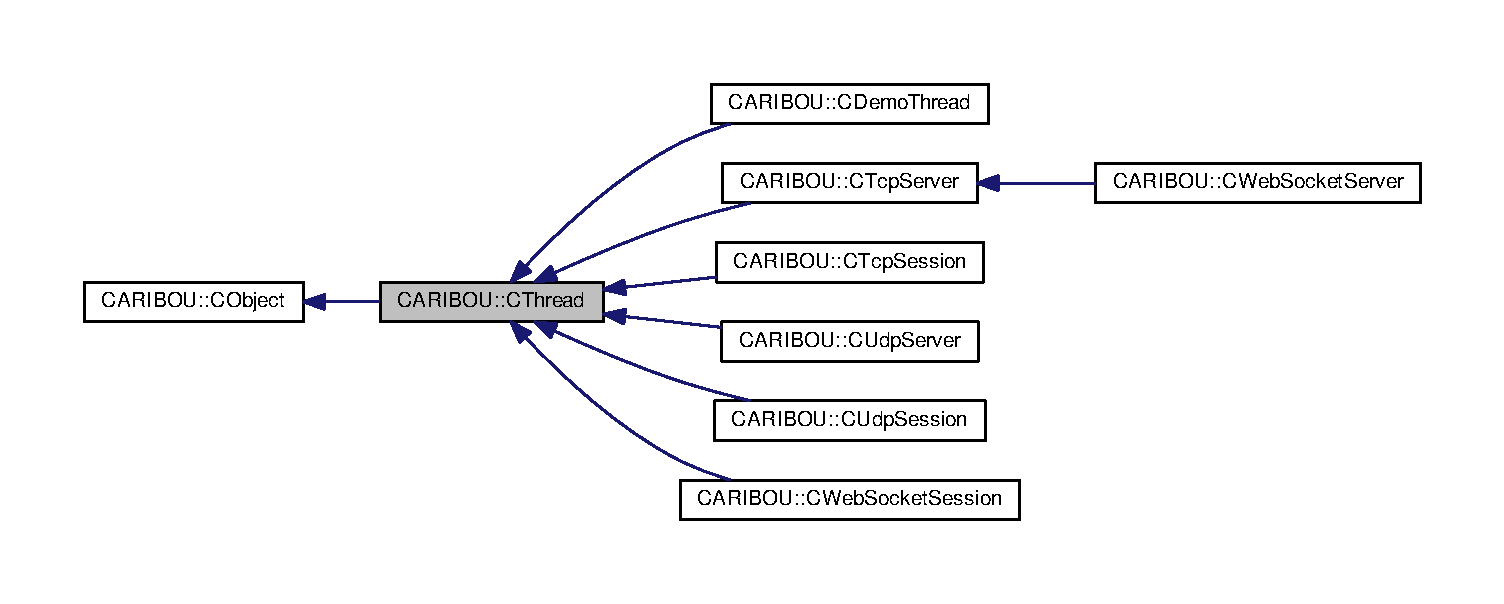
\includegraphics[width=350pt]{class_c_a_r_i_b_o_u_1_1_c_thread__inherit__graph}
\end{center}
\end{figure}


Collaboration diagram for C\+A\+R\+I\+B\+OU\+:\+:C\+Thread\+:\nopagebreak
\begin{figure}[H]
\begin{center}
\leavevmode
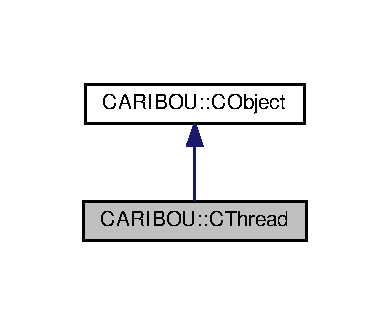
\includegraphics[width=187pt]{class_c_a_r_i_b_o_u_1_1_c_thread__coll__graph}
\end{center}
\end{figure}
\subsection*{Public Member Functions}
\begin{DoxyCompactItemize}
\item 
{\bf C\+Thread} (caribou\+\_\+thread\+\_\+t $\ast$)
\item 
{\bf C\+Thread} (const char $\ast${\bf name}, uint16\+\_\+t stksize=C\+A\+R\+I\+B\+O\+U\+\_\+\+T\+H\+R\+E\+A\+D\+\_\+\+D\+E\+F\+\_\+\+S\+T\+K\+SZ, uint16\+\_\+t {\bf priority}=C\+A\+R\+I\+B\+O\+U\+\_\+\+T\+H\+R\+E\+A\+D\+\_\+\+N\+O\+R\+M\+A\+L\+P\+R\+IO)
\item 
virtual {\bf $\sim$\+C\+Thread} ()
\item 
virtual void {\bf run} ()=0
\item 
virtual void {\bf start} ()
\item 
bool {\bf started} ()
\item 
bool {\bf finished} ()
\item 
void {\bf finish} ()
\item 
void {\bf set\+Name} (const char $\ast${\bf name})
\item 
char $\ast$ {\bf name} ()
\item 
uint64\+\_\+t {\bf runtime} ()
\item 
uint32\+\_\+t {\bf stacksize} ()
\item 
uint32\+\_\+t {\bf stackusage} ()
\item 
int16\+\_\+t {\bf priority} ()
\item 
uint16\+\_\+t {\bf state} ()
\item 
{\bf C\+String} {\bf status} ()
\item 
virtual void {\bf wakeup} ()
\begin{DoxyCompactList}\small\item\em Wake up from sleep. \end{DoxyCompactList}\item 
caribou\+\_\+thread\+\_\+t $\ast$ {\bf id} ()
\item 
caribou\+\_\+thread\+\_\+t $\ast$ {\bf parent\+Id} ()
\end{DoxyCompactItemize}
\subsection*{Static Public Member Functions}
\begin{DoxyCompactItemize}
\item 
static {\bf C\+Thread} $\ast$ {\bf current} ()
\begin{DoxyCompactList}\small\item\em Current thread must be \doxyref{lock()}{p.}{class_c_a_r_i_b_o_u_1_1_c_thread_a6e231208db98d71abd50c430432114e7}\textquotesingle{}ed before accessing \doxyref{find()}{p.}{class_c_a_r_i_b_o_u_1_1_c_thread_aa8d90ae118abb0344e64d8dbafa4d7ae}, and then \doxyref{unlock()}{p.}{class_c_a_r_i_b_o_u_1_1_c_thread_a7c861bc3a6ab2fb99c6995d943323403}\textquotesingle{}ed. \end{DoxyCompactList}\item 
static {\bf C\+Thread} $\ast$ {\bf find} (char $\ast${\bf name})
\item 
static void {\bf yield} ()
\begin{DoxyCompactList}\small\item\em Yields the time slot. \end{DoxyCompactList}\item 
static caribou\+\_\+tick\+\_\+t {\bf timer\+Ticks} ()
\begin{DoxyCompactList}\small\item\em Number of ticks elapsed. \end{DoxyCompactList}\item 
static bool {\bf timer\+Timeout} (caribou\+\_\+tick\+\_\+t {\bf start}, caribou\+\_\+tick\+\_\+t timeout)
\begin{DoxyCompactList}\small\item\em Timer timeout. \end{DoxyCompactList}\item 
static int {\bf timer\+Period} ()
\begin{DoxyCompactList}\small\item\em Number of milliseconds in a tick. \end{DoxyCompactList}\end{DoxyCompactItemize}
\subsection*{Protected Member Functions}
\begin{DoxyCompactItemize}
\item 
void {\bf set\+Watchdog\+Handle} (uint8\+\_\+t handle)
\item 
uint8\+\_\+t {\bf watchdog\+Handle} ()
\item 
virtual void {\bf lock} ()
\begin{DoxyCompactList}\small\item\em Lock the current thread. \end{DoxyCompactList}\item 
virtual void {\bf unlock} ()
\begin{DoxyCompactList}\small\item\em Unlock the current thread. \end{DoxyCompactList}\item 
virtual void {\bf sleep} (int msec=-\/1)
\begin{DoxyCompactList}\small\item\em Sleep for some milliseconds. \end{DoxyCompactList}\end{DoxyCompactItemize}
\subsection*{Additional Inherited Members}


\subsection{Detailed Description}


Definition at line 25 of file cthread.\+h.



\subsection{Constructor \& Destructor Documentation}
\index{C\+A\+R\+I\+B\+O\+U\+::\+C\+Thread@{C\+A\+R\+I\+B\+O\+U\+::\+C\+Thread}!C\+Thread@{C\+Thread}}
\index{C\+Thread@{C\+Thread}!C\+A\+R\+I\+B\+O\+U\+::\+C\+Thread@{C\+A\+R\+I\+B\+O\+U\+::\+C\+Thread}}
\subsubsection[{C\+Thread(caribou\+\_\+thread\+\_\+t $\ast$)}]{\setlength{\rightskip}{0pt plus 5cm}C\+A\+R\+I\+B\+O\+U\+::\+C\+Thread\+::\+C\+Thread (
\begin{DoxyParamCaption}
\item[{caribou\+\_\+thread\+\_\+t $\ast$}]{thread}
\end{DoxyParamCaption}
)}\label{class_c_a_r_i_b_o_u_1_1_c_thread_a2848bfb3b1114fa6924a9e13e44df7f1}


Definition at line 53 of file cthread.\+cpp.

\index{C\+A\+R\+I\+B\+O\+U\+::\+C\+Thread@{C\+A\+R\+I\+B\+O\+U\+::\+C\+Thread}!C\+Thread@{C\+Thread}}
\index{C\+Thread@{C\+Thread}!C\+A\+R\+I\+B\+O\+U\+::\+C\+Thread@{C\+A\+R\+I\+B\+O\+U\+::\+C\+Thread}}
\subsubsection[{C\+Thread(const char $\ast$name, uint16\+\_\+t stksize=\+C\+A\+R\+I\+B\+O\+U\+\_\+\+T\+H\+R\+E\+A\+D\+\_\+\+D\+E\+F\+\_\+\+S\+T\+K\+S\+Z, uint16\+\_\+t priority=\+C\+A\+R\+I\+B\+O\+U\+\_\+\+T\+H\+R\+E\+A\+D\+\_\+\+N\+O\+R\+M\+A\+L\+P\+R\+I\+O)}]{\setlength{\rightskip}{0pt plus 5cm}C\+A\+R\+I\+B\+O\+U\+::\+C\+Thread\+::\+C\+Thread (
\begin{DoxyParamCaption}
\item[{const char $\ast$}]{name, }
\item[{uint16\+\_\+t}]{stksize = {\ttfamily CARIBOU\+\_\+THREAD\+\_\+DEF\+\_\+STKSZ}, }
\item[{uint16\+\_\+t}]{priority = {\ttfamily CARIBOU\+\_\+THREAD\+\_\+NORMALPRIO}}
\end{DoxyParamCaption}
)}\label{class_c_a_r_i_b_o_u_1_1_c_thread_aee8e7baf4d3ef4c58773b325962c3eb5}


Definition at line 65 of file cthread.\+cpp.

\index{C\+A\+R\+I\+B\+O\+U\+::\+C\+Thread@{C\+A\+R\+I\+B\+O\+U\+::\+C\+Thread}!````~C\+Thread@{$\sim$\+C\+Thread}}
\index{````~C\+Thread@{$\sim$\+C\+Thread}!C\+A\+R\+I\+B\+O\+U\+::\+C\+Thread@{C\+A\+R\+I\+B\+O\+U\+::\+C\+Thread}}
\subsubsection[{$\sim$\+C\+Thread()}]{\setlength{\rightskip}{0pt plus 5cm}C\+A\+R\+I\+B\+O\+U\+::\+C\+Thread\+::$\sim$\+C\+Thread (
\begin{DoxyParamCaption}
{}
\end{DoxyParamCaption}
)\hspace{0.3cm}{\ttfamily [virtual]}}\label{class_c_a_r_i_b_o_u_1_1_c_thread_abbc20a3e8e8a6fa4de085ed9c6e4668d}


Definition at line 85 of file cthread.\+cpp.



\subsection{Member Function Documentation}
\index{C\+A\+R\+I\+B\+O\+U\+::\+C\+Thread@{C\+A\+R\+I\+B\+O\+U\+::\+C\+Thread}!current@{current}}
\index{current@{current}!C\+A\+R\+I\+B\+O\+U\+::\+C\+Thread@{C\+A\+R\+I\+B\+O\+U\+::\+C\+Thread}}
\subsubsection[{current()}]{\setlength{\rightskip}{0pt plus 5cm}{\bf C\+Thread} $\ast$ C\+A\+R\+I\+B\+O\+U\+::\+C\+Thread\+::current (
\begin{DoxyParamCaption}
{}
\end{DoxyParamCaption}
)\hspace{0.3cm}{\ttfamily [static]}}\label{class_c_a_r_i_b_o_u_1_1_c_thread_a572cbd902b395fefcebfd5bcacd04cf2}


Current thread must be \doxyref{lock()}{p.}{class_c_a_r_i_b_o_u_1_1_c_thread_a6e231208db98d71abd50c430432114e7}\textquotesingle{}ed before accessing \doxyref{find()}{p.}{class_c_a_r_i_b_o_u_1_1_c_thread_aa8d90ae118abb0344e64d8dbafa4d7ae}, and then \doxyref{unlock()}{p.}{class_c_a_r_i_b_o_u_1_1_c_thread_a7c861bc3a6ab2fb99c6995d943323403}\textquotesingle{}ed. 

\begin{DoxyReturn}{Returns}
find a thread by name 

Get the current arg. N\+U\+LL indicates main thread (main thread is not a \doxyref{C\+Thread}{p.}{class_c_a_r_i_b_o_u_1_1_c_thread}). 
\end{DoxyReturn}


Definition at line 134 of file cthread.\+cpp.

\index{C\+A\+R\+I\+B\+O\+U\+::\+C\+Thread@{C\+A\+R\+I\+B\+O\+U\+::\+C\+Thread}!find@{find}}
\index{find@{find}!C\+A\+R\+I\+B\+O\+U\+::\+C\+Thread@{C\+A\+R\+I\+B\+O\+U\+::\+C\+Thread}}
\subsubsection[{find(char $\ast$name)}]{\setlength{\rightskip}{0pt plus 5cm}static {\bf C\+Thread}$\ast$ C\+A\+R\+I\+B\+O\+U\+::\+C\+Thread\+::find (
\begin{DoxyParamCaption}
\item[{char $\ast$}]{name}
\end{DoxyParamCaption}
)\hspace{0.3cm}{\ttfamily [static]}}\label{class_c_a_r_i_b_o_u_1_1_c_thread_aa8d90ae118abb0344e64d8dbafa4d7ae}
\index{C\+A\+R\+I\+B\+O\+U\+::\+C\+Thread@{C\+A\+R\+I\+B\+O\+U\+::\+C\+Thread}!finish@{finish}}
\index{finish@{finish}!C\+A\+R\+I\+B\+O\+U\+::\+C\+Thread@{C\+A\+R\+I\+B\+O\+U\+::\+C\+Thread}}
\subsubsection[{finish()}]{\setlength{\rightskip}{0pt plus 5cm}void C\+A\+R\+I\+B\+O\+U\+::\+C\+Thread\+::finish (
\begin{DoxyParamCaption}
{}
\end{DoxyParamCaption}
)\hspace{0.3cm}{\ttfamily [inline]}}\label{class_c_a_r_i_b_o_u_1_1_c_thread_a48eff79fbf8ac1882a8cde486784eecc}


Definition at line 37 of file cthread.\+h.

\index{C\+A\+R\+I\+B\+O\+U\+::\+C\+Thread@{C\+A\+R\+I\+B\+O\+U\+::\+C\+Thread}!finished@{finished}}
\index{finished@{finished}!C\+A\+R\+I\+B\+O\+U\+::\+C\+Thread@{C\+A\+R\+I\+B\+O\+U\+::\+C\+Thread}}
\subsubsection[{finished()}]{\setlength{\rightskip}{0pt plus 5cm}bool C\+A\+R\+I\+B\+O\+U\+::\+C\+Thread\+::finished (
\begin{DoxyParamCaption}
{}
\end{DoxyParamCaption}
)\hspace{0.3cm}{\ttfamily [inline]}}\label{class_c_a_r_i_b_o_u_1_1_c_thread_af47b7f67dca88fb16852600319c53fc7}


Definition at line 36 of file cthread.\+h.

\index{C\+A\+R\+I\+B\+O\+U\+::\+C\+Thread@{C\+A\+R\+I\+B\+O\+U\+::\+C\+Thread}!id@{id}}
\index{id@{id}!C\+A\+R\+I\+B\+O\+U\+::\+C\+Thread@{C\+A\+R\+I\+B\+O\+U\+::\+C\+Thread}}
\subsubsection[{id()}]{\setlength{\rightskip}{0pt plus 5cm}caribou\+\_\+thread\+\_\+t$\ast$ C\+A\+R\+I\+B\+O\+U\+::\+C\+Thread\+::id (
\begin{DoxyParamCaption}
{}
\end{DoxyParamCaption}
)\hspace{0.3cm}{\ttfamily [inline]}}\label{class_c_a_r_i_b_o_u_1_1_c_thread_ab052e15d54235546b1fdb66b3f6cd92a}


Definition at line 48 of file cthread.\+h.

\index{C\+A\+R\+I\+B\+O\+U\+::\+C\+Thread@{C\+A\+R\+I\+B\+O\+U\+::\+C\+Thread}!lock@{lock}}
\index{lock@{lock}!C\+A\+R\+I\+B\+O\+U\+::\+C\+Thread@{C\+A\+R\+I\+B\+O\+U\+::\+C\+Thread}}
\subsubsection[{lock()}]{\setlength{\rightskip}{0pt plus 5cm}void C\+A\+R\+I\+B\+O\+U\+::\+C\+Thread\+::lock (
\begin{DoxyParamCaption}
{}
\end{DoxyParamCaption}
)\hspace{0.3cm}{\ttfamily [protected]}, {\ttfamily [virtual]}}\label{class_c_a_r_i_b_o_u_1_1_c_thread_a6e231208db98d71abd50c430432114e7}


Lock the current thread. 



Definition at line 171 of file cthread.\+cpp.

\index{C\+A\+R\+I\+B\+O\+U\+::\+C\+Thread@{C\+A\+R\+I\+B\+O\+U\+::\+C\+Thread}!name@{name}}
\index{name@{name}!C\+A\+R\+I\+B\+O\+U\+::\+C\+Thread@{C\+A\+R\+I\+B\+O\+U\+::\+C\+Thread}}
\subsubsection[{name()}]{\setlength{\rightskip}{0pt plus 5cm}char $\ast$ C\+A\+R\+I\+B\+O\+U\+::\+C\+Thread\+::name (
\begin{DoxyParamCaption}
{}
\end{DoxyParamCaption}
)}\label{class_c_a_r_i_b_o_u_1_1_c_thread_ae1bde2cdc36e6c36b6324dde3f30f503}
\begin{DoxyReturn}{Returns}
the name of the thread. 
\end{DoxyReturn}


Definition at line 104 of file cthread.\+cpp.

\index{C\+A\+R\+I\+B\+O\+U\+::\+C\+Thread@{C\+A\+R\+I\+B\+O\+U\+::\+C\+Thread}!parent\+Id@{parent\+Id}}
\index{parent\+Id@{parent\+Id}!C\+A\+R\+I\+B\+O\+U\+::\+C\+Thread@{C\+A\+R\+I\+B\+O\+U\+::\+C\+Thread}}
\subsubsection[{parent\+Id()}]{\setlength{\rightskip}{0pt plus 5cm}caribou\+\_\+thread\+\_\+t$\ast$ C\+A\+R\+I\+B\+O\+U\+::\+C\+Thread\+::parent\+Id (
\begin{DoxyParamCaption}
{}
\end{DoxyParamCaption}
)\hspace{0.3cm}{\ttfamily [inline]}}\label{class_c_a_r_i_b_o_u_1_1_c_thread_aeb4340ea6b83cd2eff270bb7a225f9de}


Definition at line 49 of file cthread.\+h.

\index{C\+A\+R\+I\+B\+O\+U\+::\+C\+Thread@{C\+A\+R\+I\+B\+O\+U\+::\+C\+Thread}!priority@{priority}}
\index{priority@{priority}!C\+A\+R\+I\+B\+O\+U\+::\+C\+Thread@{C\+A\+R\+I\+B\+O\+U\+::\+C\+Thread}}
\subsubsection[{priority()}]{\setlength{\rightskip}{0pt plus 5cm}int16\+\_\+t C\+A\+R\+I\+B\+O\+U\+::\+C\+Thread\+::priority (
\begin{DoxyParamCaption}
{}
\end{DoxyParamCaption}
)}\label{class_c_a_r_i_b_o_u_1_1_c_thread_a8d6c99c5e0182c755727e6195c142905}


Definition at line 202 of file cthread.\+cpp.

\index{C\+A\+R\+I\+B\+O\+U\+::\+C\+Thread@{C\+A\+R\+I\+B\+O\+U\+::\+C\+Thread}!run@{run}}
\index{run@{run}!C\+A\+R\+I\+B\+O\+U\+::\+C\+Thread@{C\+A\+R\+I\+B\+O\+U\+::\+C\+Thread}}
\subsubsection[{run()=0}]{\setlength{\rightskip}{0pt plus 5cm}virtual void C\+A\+R\+I\+B\+O\+U\+::\+C\+Thread\+::run (
\begin{DoxyParamCaption}
{}
\end{DoxyParamCaption}
)\hspace{0.3cm}{\ttfamily [pure virtual]}}\label{class_c_a_r_i_b_o_u_1_1_c_thread_a087ae48a158aca84892aea7f9ed16711}


Implemented in {\bf C\+A\+R\+I\+B\+O\+U\+::\+C\+Tcp\+Server} \doxyref{}{p.}{class_c_a_r_i_b_o_u_1_1_c_tcp_server_a4d38415ea32f02035266cb34433ff392}, {\bf C\+A\+R\+I\+B\+O\+U\+::\+C\+Udp\+Server} \doxyref{}{p.}{class_c_a_r_i_b_o_u_1_1_c_udp_server_a57eefe6dd725771c49ca33eb332fd291}, {\bf C\+A\+R\+I\+B\+O\+U\+::\+C\+Udp\+Session} \doxyref{}{p.}{class_c_a_r_i_b_o_u_1_1_c_udp_session_a59a2d243c8d8ad6dc08ce93b9b6fb712}, {\bf C\+A\+R\+I\+B\+O\+U\+::\+C\+Web\+Socket\+Server} \doxyref{}{p.}{class_c_a_r_i_b_o_u_1_1_c_web_socket_server_a92d612844ad0295da21ebd0834ad5dc2}, {\bf C\+A\+R\+I\+B\+O\+U\+::\+C\+Tcp\+Session} \doxyref{}{p.}{class_c_a_r_i_b_o_u_1_1_c_tcp_session_a66d1ace1fb86d1f41c587aff037adc12}, {\bf C\+A\+R\+I\+B\+O\+U\+::\+C\+Web\+Socket\+Session} \doxyref{}{p.}{class_c_a_r_i_b_o_u_1_1_c_web_socket_session_a6aa2f8ca1466780fb76a018b17f099b7}, and {\bf C\+A\+R\+I\+B\+O\+U\+::\+C\+Demo\+Thread} \doxyref{}{p.}{class_c_a_r_i_b_o_u_1_1_c_demo_thread_a8d2763e9b70a9ecb17b0da5b8f3d7eb0}.

\index{C\+A\+R\+I\+B\+O\+U\+::\+C\+Thread@{C\+A\+R\+I\+B\+O\+U\+::\+C\+Thread}!runtime@{runtime}}
\index{runtime@{runtime}!C\+A\+R\+I\+B\+O\+U\+::\+C\+Thread@{C\+A\+R\+I\+B\+O\+U\+::\+C\+Thread}}
\subsubsection[{runtime()}]{\setlength{\rightskip}{0pt plus 5cm}uint64\+\_\+t C\+A\+R\+I\+B\+O\+U\+::\+C\+Thread\+::runtime (
\begin{DoxyParamCaption}
{}
\end{DoxyParamCaption}
)}\label{class_c_a_r_i_b_o_u_1_1_c_thread_a809adadbb3ae88742d4057bd2af044da}
\begin{DoxyReturn}{Returns}
runtime in milliseconds 
\end{DoxyReturn}


Definition at line 187 of file cthread.\+cpp.

\index{C\+A\+R\+I\+B\+O\+U\+::\+C\+Thread@{C\+A\+R\+I\+B\+O\+U\+::\+C\+Thread}!set\+Name@{set\+Name}}
\index{set\+Name@{set\+Name}!C\+A\+R\+I\+B\+O\+U\+::\+C\+Thread@{C\+A\+R\+I\+B\+O\+U\+::\+C\+Thread}}
\subsubsection[{set\+Name(const char $\ast$name)}]{\setlength{\rightskip}{0pt plus 5cm}void C\+A\+R\+I\+B\+O\+U\+::\+C\+Thread\+::set\+Name (
\begin{DoxyParamCaption}
\item[{const char $\ast$}]{name}
\end{DoxyParamCaption}
)}\label{class_c_a_r_i_b_o_u_1_1_c_thread_acb2bbc3b0bd9a479005f9b67fb1c26cc}


Definition at line 96 of file cthread.\+cpp.

\index{C\+A\+R\+I\+B\+O\+U\+::\+C\+Thread@{C\+A\+R\+I\+B\+O\+U\+::\+C\+Thread}!set\+Watchdog\+Handle@{set\+Watchdog\+Handle}}
\index{set\+Watchdog\+Handle@{set\+Watchdog\+Handle}!C\+A\+R\+I\+B\+O\+U\+::\+C\+Thread@{C\+A\+R\+I\+B\+O\+U\+::\+C\+Thread}}
\subsubsection[{set\+Watchdog\+Handle(uint8\+\_\+t handle)}]{\setlength{\rightskip}{0pt plus 5cm}void C\+A\+R\+I\+B\+O\+U\+::\+C\+Thread\+::set\+Watchdog\+Handle (
\begin{DoxyParamCaption}
\item[{uint8\+\_\+t}]{handle}
\end{DoxyParamCaption}
)\hspace{0.3cm}{\ttfamily [inline]}, {\ttfamily [protected]}}\label{class_c_a_r_i_b_o_u_1_1_c_thread_a7464b795f4a90ac66258cb69699bfc23}


Definition at line 65 of file cthread.\+h.

\index{C\+A\+R\+I\+B\+O\+U\+::\+C\+Thread@{C\+A\+R\+I\+B\+O\+U\+::\+C\+Thread}!sleep@{sleep}}
\index{sleep@{sleep}!C\+A\+R\+I\+B\+O\+U\+::\+C\+Thread@{C\+A\+R\+I\+B\+O\+U\+::\+C\+Thread}}
\subsubsection[{sleep(int msec=-\/1)}]{\setlength{\rightskip}{0pt plus 5cm}void C\+A\+R\+I\+B\+O\+U\+::\+C\+Thread\+::sleep (
\begin{DoxyParamCaption}
\item[{int}]{msec = {\ttfamily -\/1}}
\end{DoxyParamCaption}
)\hspace{0.3cm}{\ttfamily [protected]}, {\ttfamily [virtual]}}\label{class_c_a_r_i_b_o_u_1_1_c_thread_afe90777479ddbf2d5024929c84406709}


Sleep for some milliseconds. 



Definition at line 150 of file cthread.\+cpp.

\index{C\+A\+R\+I\+B\+O\+U\+::\+C\+Thread@{C\+A\+R\+I\+B\+O\+U\+::\+C\+Thread}!stacksize@{stacksize}}
\index{stacksize@{stacksize}!C\+A\+R\+I\+B\+O\+U\+::\+C\+Thread@{C\+A\+R\+I\+B\+O\+U\+::\+C\+Thread}}
\subsubsection[{stacksize()}]{\setlength{\rightskip}{0pt plus 5cm}uint32\+\_\+t C\+A\+R\+I\+B\+O\+U\+::\+C\+Thread\+::stacksize (
\begin{DoxyParamCaption}
{}
\end{DoxyParamCaption}
)}\label{class_c_a_r_i_b_o_u_1_1_c_thread_a298e39cfbe891d5e782f6addb2ecd363}


Definition at line 192 of file cthread.\+cpp.

\index{C\+A\+R\+I\+B\+O\+U\+::\+C\+Thread@{C\+A\+R\+I\+B\+O\+U\+::\+C\+Thread}!stackusage@{stackusage}}
\index{stackusage@{stackusage}!C\+A\+R\+I\+B\+O\+U\+::\+C\+Thread@{C\+A\+R\+I\+B\+O\+U\+::\+C\+Thread}}
\subsubsection[{stackusage()}]{\setlength{\rightskip}{0pt plus 5cm}uint32\+\_\+t C\+A\+R\+I\+B\+O\+U\+::\+C\+Thread\+::stackusage (
\begin{DoxyParamCaption}
{}
\end{DoxyParamCaption}
)}\label{class_c_a_r_i_b_o_u_1_1_c_thread_aa888d43a22a1c749bb54773fd6691157}


Definition at line 197 of file cthread.\+cpp.

\index{C\+A\+R\+I\+B\+O\+U\+::\+C\+Thread@{C\+A\+R\+I\+B\+O\+U\+::\+C\+Thread}!start@{start}}
\index{start@{start}!C\+A\+R\+I\+B\+O\+U\+::\+C\+Thread@{C\+A\+R\+I\+B\+O\+U\+::\+C\+Thread}}
\subsubsection[{start()}]{\setlength{\rightskip}{0pt plus 5cm}virtual void C\+A\+R\+I\+B\+O\+U\+::\+C\+Thread\+::start (
\begin{DoxyParamCaption}
{}
\end{DoxyParamCaption}
)\hspace{0.3cm}{\ttfamily [inline]}, {\ttfamily [virtual]}}\label{class_c_a_r_i_b_o_u_1_1_c_thread_abeda7f131ee1d3d66f0780e9e79ab112}


Definition at line 33 of file cthread.\+h.

\index{C\+A\+R\+I\+B\+O\+U\+::\+C\+Thread@{C\+A\+R\+I\+B\+O\+U\+::\+C\+Thread}!started@{started}}
\index{started@{started}!C\+A\+R\+I\+B\+O\+U\+::\+C\+Thread@{C\+A\+R\+I\+B\+O\+U\+::\+C\+Thread}}
\subsubsection[{started()}]{\setlength{\rightskip}{0pt plus 5cm}bool C\+A\+R\+I\+B\+O\+U\+::\+C\+Thread\+::started (
\begin{DoxyParamCaption}
{}
\end{DoxyParamCaption}
)\hspace{0.3cm}{\ttfamily [inline]}}\label{class_c_a_r_i_b_o_u_1_1_c_thread_a6d4b9072f806f604477cb83b0dd391d2}


Definition at line 35 of file cthread.\+h.

\index{C\+A\+R\+I\+B\+O\+U\+::\+C\+Thread@{C\+A\+R\+I\+B\+O\+U\+::\+C\+Thread}!state@{state}}
\index{state@{state}!C\+A\+R\+I\+B\+O\+U\+::\+C\+Thread@{C\+A\+R\+I\+B\+O\+U\+::\+C\+Thread}}
\subsubsection[{state()}]{\setlength{\rightskip}{0pt plus 5cm}uint16\+\_\+t C\+A\+R\+I\+B\+O\+U\+::\+C\+Thread\+::state (
\begin{DoxyParamCaption}
{}
\end{DoxyParamCaption}
)}\label{class_c_a_r_i_b_o_u_1_1_c_thread_aa6120054f575ffe53d4aba7369b9ed5f}


Definition at line 207 of file cthread.\+cpp.

\index{C\+A\+R\+I\+B\+O\+U\+::\+C\+Thread@{C\+A\+R\+I\+B\+O\+U\+::\+C\+Thread}!status@{status}}
\index{status@{status}!C\+A\+R\+I\+B\+O\+U\+::\+C\+Thread@{C\+A\+R\+I\+B\+O\+U\+::\+C\+Thread}}
\subsubsection[{status()}]{\setlength{\rightskip}{0pt plus 5cm}{\bf C\+String} C\+A\+R\+I\+B\+O\+U\+::\+C\+Thread\+::status (
\begin{DoxyParamCaption}
{}
\end{DoxyParamCaption}
)}\label{class_c_a_r_i_b_o_u_1_1_c_thread_a89c47b43c277c5c5d855b73e0418d74d}


Definition at line 212 of file cthread.\+cpp.

\index{C\+A\+R\+I\+B\+O\+U\+::\+C\+Thread@{C\+A\+R\+I\+B\+O\+U\+::\+C\+Thread}!timer\+Period@{timer\+Period}}
\index{timer\+Period@{timer\+Period}!C\+A\+R\+I\+B\+O\+U\+::\+C\+Thread@{C\+A\+R\+I\+B\+O\+U\+::\+C\+Thread}}
\subsubsection[{timer\+Period()}]{\setlength{\rightskip}{0pt plus 5cm}int C\+A\+R\+I\+B\+O\+U\+::\+C\+Thread\+::timer\+Period (
\begin{DoxyParamCaption}
{}
\end{DoxyParamCaption}
)\hspace{0.3cm}{\ttfamily [static]}}\label{class_c_a_r_i_b_o_u_1_1_c_thread_a984919b6ad60b0213c57669fd6b4bf89}


Number of milliseconds in a tick. 



Definition at line 234 of file cthread.\+cpp.

\index{C\+A\+R\+I\+B\+O\+U\+::\+C\+Thread@{C\+A\+R\+I\+B\+O\+U\+::\+C\+Thread}!timer\+Ticks@{timer\+Ticks}}
\index{timer\+Ticks@{timer\+Ticks}!C\+A\+R\+I\+B\+O\+U\+::\+C\+Thread@{C\+A\+R\+I\+B\+O\+U\+::\+C\+Thread}}
\subsubsection[{timer\+Ticks()}]{\setlength{\rightskip}{0pt plus 5cm}caribou\+\_\+tick\+\_\+t C\+A\+R\+I\+B\+O\+U\+::\+C\+Thread\+::timer\+Ticks (
\begin{DoxyParamCaption}
{}
\end{DoxyParamCaption}
)\hspace{0.3cm}{\ttfamily [static]}}\label{class_c_a_r_i_b_o_u_1_1_c_thread_ab05b0426ac736e59650b644353787431}


Number of ticks elapsed. 



Definition at line 226 of file cthread.\+cpp.

\index{C\+A\+R\+I\+B\+O\+U\+::\+C\+Thread@{C\+A\+R\+I\+B\+O\+U\+::\+C\+Thread}!timer\+Timeout@{timer\+Timeout}}
\index{timer\+Timeout@{timer\+Timeout}!C\+A\+R\+I\+B\+O\+U\+::\+C\+Thread@{C\+A\+R\+I\+B\+O\+U\+::\+C\+Thread}}
\subsubsection[{timer\+Timeout(caribou\+\_\+tick\+\_\+t start, caribou\+\_\+tick\+\_\+t timeout)}]{\setlength{\rightskip}{0pt plus 5cm}bool C\+A\+R\+I\+B\+O\+U\+::\+C\+Thread\+::timer\+Timeout (
\begin{DoxyParamCaption}
\item[{caribou\+\_\+tick\+\_\+t}]{start, }
\item[{caribou\+\_\+tick\+\_\+t}]{timeout}
\end{DoxyParamCaption}
)\hspace{0.3cm}{\ttfamily [static]}}\label{class_c_a_r_i_b_o_u_1_1_c_thread_ac1c427f7fd996c430ece1db3d88c7822}


Timer timeout. 



Definition at line 242 of file cthread.\+cpp.

\index{C\+A\+R\+I\+B\+O\+U\+::\+C\+Thread@{C\+A\+R\+I\+B\+O\+U\+::\+C\+Thread}!unlock@{unlock}}
\index{unlock@{unlock}!C\+A\+R\+I\+B\+O\+U\+::\+C\+Thread@{C\+A\+R\+I\+B\+O\+U\+::\+C\+Thread}}
\subsubsection[{unlock()}]{\setlength{\rightskip}{0pt plus 5cm}void C\+A\+R\+I\+B\+O\+U\+::\+C\+Thread\+::unlock (
\begin{DoxyParamCaption}
{}
\end{DoxyParamCaption}
)\hspace{0.3cm}{\ttfamily [protected]}, {\ttfamily [virtual]}}\label{class_c_a_r_i_b_o_u_1_1_c_thread_a7c861bc3a6ab2fb99c6995d943323403}


Unlock the current thread. 



Definition at line 179 of file cthread.\+cpp.

\index{C\+A\+R\+I\+B\+O\+U\+::\+C\+Thread@{C\+A\+R\+I\+B\+O\+U\+::\+C\+Thread}!wakeup@{wakeup}}
\index{wakeup@{wakeup}!C\+A\+R\+I\+B\+O\+U\+::\+C\+Thread@{C\+A\+R\+I\+B\+O\+U\+::\+C\+Thread}}
\subsubsection[{wakeup()}]{\setlength{\rightskip}{0pt plus 5cm}void C\+A\+R\+I\+B\+O\+U\+::\+C\+Thread\+::wakeup (
\begin{DoxyParamCaption}
{}
\end{DoxyParamCaption}
)\hspace{0.3cm}{\ttfamily [virtual]}}\label{class_c_a_r_i_b_o_u_1_1_c_thread_a2257348700522c9bd56756cb6f2b2ed8}


Wake up from sleep. 



Definition at line 163 of file cthread.\+cpp.

\index{C\+A\+R\+I\+B\+O\+U\+::\+C\+Thread@{C\+A\+R\+I\+B\+O\+U\+::\+C\+Thread}!watchdog\+Handle@{watchdog\+Handle}}
\index{watchdog\+Handle@{watchdog\+Handle}!C\+A\+R\+I\+B\+O\+U\+::\+C\+Thread@{C\+A\+R\+I\+B\+O\+U\+::\+C\+Thread}}
\subsubsection[{watchdog\+Handle()}]{\setlength{\rightskip}{0pt plus 5cm}uint8\+\_\+t C\+A\+R\+I\+B\+O\+U\+::\+C\+Thread\+::watchdog\+Handle (
\begin{DoxyParamCaption}
{}
\end{DoxyParamCaption}
)\hspace{0.3cm}{\ttfamily [inline]}, {\ttfamily [protected]}}\label{class_c_a_r_i_b_o_u_1_1_c_thread_adae2f4ee7d1d6df80fa1f3b9807cb6a6}


Definition at line 66 of file cthread.\+h.

\index{C\+A\+R\+I\+B\+O\+U\+::\+C\+Thread@{C\+A\+R\+I\+B\+O\+U\+::\+C\+Thread}!yield@{yield}}
\index{yield@{yield}!C\+A\+R\+I\+B\+O\+U\+::\+C\+Thread@{C\+A\+R\+I\+B\+O\+U\+::\+C\+Thread}}
\subsubsection[{yield()}]{\setlength{\rightskip}{0pt plus 5cm}void C\+A\+R\+I\+B\+O\+U\+::\+C\+Thread\+::yield (
\begin{DoxyParamCaption}
{}
\end{DoxyParamCaption}
)\hspace{0.3cm}{\ttfamily [static]}}\label{class_c_a_r_i_b_o_u_1_1_c_thread_aab29ddbc9e5c051ab9a4edd748384624}


Yields the time slot. 



Definition at line 142 of file cthread.\+cpp.



The documentation for this class was generated from the following files\+:\begin{DoxyCompactItemize}
\item 
include/caribou++/{\bf cthread.\+h}\item 
src/{\bf cthread.\+cpp}\end{DoxyCompactItemize}

\section{C\-A\-R\-I\-B\-O\-U\-:\-:C\-Timer\-Event Class Reference}
\label{class_c_a_r_i_b_o_u_1_1_c_timer_event}\index{C\-A\-R\-I\-B\-O\-U\-::\-C\-Timer\-Event@{C\-A\-R\-I\-B\-O\-U\-::\-C\-Timer\-Event}}


{\ttfamily \#include $<$ctimerevent.\-h$>$}



Inheritance diagram for C\-A\-R\-I\-B\-O\-U\-:\-:C\-Timer\-Event\-:\nopagebreak
\begin{figure}[H]
\begin{center}
\leavevmode
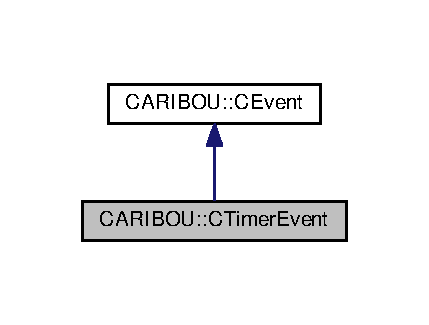
\includegraphics[width=206pt]{class_c_a_r_i_b_o_u_1_1_c_timer_event__inherit__graph}
\end{center}
\end{figure}


Collaboration diagram for C\-A\-R\-I\-B\-O\-U\-:\-:C\-Timer\-Event\-:\nopagebreak
\begin{figure}[H]
\begin{center}
\leavevmode
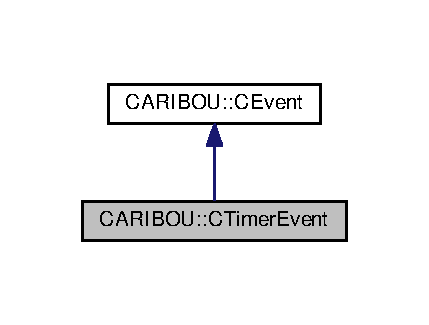
\includegraphics[width=206pt]{class_c_a_r_i_b_o_u_1_1_c_timer_event__coll__graph}
\end{center}
\end{figure}
\subsection*{Public Member Functions}
\begin{DoxyCompactItemize}
\item 
{\bf C\-Timer\-Event} ()
\item 
{\bf C\-Timer\-Event} ({\bf C\-Object} $\ast${\bf sender}, void $\ast$timer)
\item 
{\bf C\-Timer\-Event} ({\bf C\-Timer\-Event} $\ast$other)
\item 
{\bf C\-Timer\-Event} ({\bf C\-Timer\-Event} \&other)
\item 
virtual {\bf $\sim$\-C\-Timer\-Event} ()
\item 
virtual void {\bf copy} ({\bf C\-Timer\-Event} \&other)
\item 
void {\bf set\-Timer\-Id} (void $\ast${\bf timer\-Id})
\item 
void $\ast$ {\bf timer\-Id} ()
\end{DoxyCompactItemize}
\subsection*{Additional Inherited Members}


\subsection{Detailed Description}


Definition at line 24 of file ctimerevent.\-h.



\subsection{Constructor \& Destructor Documentation}
\index{C\-A\-R\-I\-B\-O\-U\-::\-C\-Timer\-Event@{C\-A\-R\-I\-B\-O\-U\-::\-C\-Timer\-Event}!C\-Timer\-Event@{C\-Timer\-Event}}
\index{C\-Timer\-Event@{C\-Timer\-Event}!CARIBOU::CTimerEvent@{C\-A\-R\-I\-B\-O\-U\-::\-C\-Timer\-Event}}
\subsubsection[{C\-Timer\-Event}]{\setlength{\rightskip}{0pt plus 5cm}C\-A\-R\-I\-B\-O\-U\-::\-C\-Timer\-Event\-::\-C\-Timer\-Event (
\begin{DoxyParamCaption}
{}
\end{DoxyParamCaption}
)}\label{class_c_a_r_i_b_o_u_1_1_c_timer_event_a3554dab55a74cab09e98c2c2793fa7e0}


Definition at line 24 of file ctimerevent.\-cpp.

\index{C\-A\-R\-I\-B\-O\-U\-::\-C\-Timer\-Event@{C\-A\-R\-I\-B\-O\-U\-::\-C\-Timer\-Event}!C\-Timer\-Event@{C\-Timer\-Event}}
\index{C\-Timer\-Event@{C\-Timer\-Event}!CARIBOU::CTimerEvent@{C\-A\-R\-I\-B\-O\-U\-::\-C\-Timer\-Event}}
\subsubsection[{C\-Timer\-Event}]{\setlength{\rightskip}{0pt plus 5cm}C\-A\-R\-I\-B\-O\-U\-::\-C\-Timer\-Event\-::\-C\-Timer\-Event (
\begin{DoxyParamCaption}
\item[{{\bf C\-Object} $\ast$}]{sender, }
\item[{void $\ast$}]{timer}
\end{DoxyParamCaption}
)}\label{class_c_a_r_i_b_o_u_1_1_c_timer_event_a02a527b2d4b01660bac39ea2907b8311}


Definition at line 31 of file ctimerevent.\-cpp.

\index{C\-A\-R\-I\-B\-O\-U\-::\-C\-Timer\-Event@{C\-A\-R\-I\-B\-O\-U\-::\-C\-Timer\-Event}!C\-Timer\-Event@{C\-Timer\-Event}}
\index{C\-Timer\-Event@{C\-Timer\-Event}!CARIBOU::CTimerEvent@{C\-A\-R\-I\-B\-O\-U\-::\-C\-Timer\-Event}}
\subsubsection[{C\-Timer\-Event}]{\setlength{\rightskip}{0pt plus 5cm}C\-A\-R\-I\-B\-O\-U\-::\-C\-Timer\-Event\-::\-C\-Timer\-Event (
\begin{DoxyParamCaption}
\item[{{\bf C\-Timer\-Event} $\ast$}]{other}
\end{DoxyParamCaption}
)\hspace{0.3cm}{\ttfamily [inline]}}\label{class_c_a_r_i_b_o_u_1_1_c_timer_event_a5f0a15a70d56f2dbd53babef644d57b7}


Definition at line 29 of file ctimerevent.\-h.

\index{C\-A\-R\-I\-B\-O\-U\-::\-C\-Timer\-Event@{C\-A\-R\-I\-B\-O\-U\-::\-C\-Timer\-Event}!C\-Timer\-Event@{C\-Timer\-Event}}
\index{C\-Timer\-Event@{C\-Timer\-Event}!CARIBOU::CTimerEvent@{C\-A\-R\-I\-B\-O\-U\-::\-C\-Timer\-Event}}
\subsubsection[{C\-Timer\-Event}]{\setlength{\rightskip}{0pt plus 5cm}C\-A\-R\-I\-B\-O\-U\-::\-C\-Timer\-Event\-::\-C\-Timer\-Event (
\begin{DoxyParamCaption}
\item[{{\bf C\-Timer\-Event} \&}]{other}
\end{DoxyParamCaption}
)\hspace{0.3cm}{\ttfamily [inline]}}\label{class_c_a_r_i_b_o_u_1_1_c_timer_event_a94c6e24d78b2ad105bc9cdafcdc44d27}


Definition at line 30 of file ctimerevent.\-h.

\index{C\-A\-R\-I\-B\-O\-U\-::\-C\-Timer\-Event@{C\-A\-R\-I\-B\-O\-U\-::\-C\-Timer\-Event}!$\sim$\-C\-Timer\-Event@{$\sim$\-C\-Timer\-Event}}
\index{$\sim$\-C\-Timer\-Event@{$\sim$\-C\-Timer\-Event}!CARIBOU::CTimerEvent@{C\-A\-R\-I\-B\-O\-U\-::\-C\-Timer\-Event}}
\subsubsection[{$\sim$\-C\-Timer\-Event}]{\setlength{\rightskip}{0pt plus 5cm}C\-A\-R\-I\-B\-O\-U\-::\-C\-Timer\-Event\-::$\sim$\-C\-Timer\-Event (
\begin{DoxyParamCaption}
{}
\end{DoxyParamCaption}
)\hspace{0.3cm}{\ttfamily [virtual]}}\label{class_c_a_r_i_b_o_u_1_1_c_timer_event_a0c39c0b539f08765dab83bf1912fe2d5}


Definition at line 38 of file ctimerevent.\-cpp.



\subsection{Member Function Documentation}
\index{C\-A\-R\-I\-B\-O\-U\-::\-C\-Timer\-Event@{C\-A\-R\-I\-B\-O\-U\-::\-C\-Timer\-Event}!copy@{copy}}
\index{copy@{copy}!CARIBOU::CTimerEvent@{C\-A\-R\-I\-B\-O\-U\-::\-C\-Timer\-Event}}
\subsubsection[{copy}]{\setlength{\rightskip}{0pt plus 5cm}void C\-A\-R\-I\-B\-O\-U\-::\-C\-Timer\-Event\-::copy (
\begin{DoxyParamCaption}
\item[{{\bf C\-Timer\-Event} \&}]{other}
\end{DoxyParamCaption}
)\hspace{0.3cm}{\ttfamily [virtual]}}\label{class_c_a_r_i_b_o_u_1_1_c_timer_event_a45ebe265d682afdce9ed2731aac2c3ba}


Definition at line 42 of file ctimerevent.\-cpp.

\index{C\-A\-R\-I\-B\-O\-U\-::\-C\-Timer\-Event@{C\-A\-R\-I\-B\-O\-U\-::\-C\-Timer\-Event}!set\-Timer\-Id@{set\-Timer\-Id}}
\index{set\-Timer\-Id@{set\-Timer\-Id}!CARIBOU::CTimerEvent@{C\-A\-R\-I\-B\-O\-U\-::\-C\-Timer\-Event}}
\subsubsection[{set\-Timer\-Id}]{\setlength{\rightskip}{0pt plus 5cm}void C\-A\-R\-I\-B\-O\-U\-::\-C\-Timer\-Event\-::set\-Timer\-Id (
\begin{DoxyParamCaption}
\item[{void $\ast$}]{timer\-Id}
\end{DoxyParamCaption}
)\hspace{0.3cm}{\ttfamily [inline]}}\label{class_c_a_r_i_b_o_u_1_1_c_timer_event_a65f47c2f61a13022265ec9e72e9298aa}


Definition at line 34 of file ctimerevent.\-h.

\index{C\-A\-R\-I\-B\-O\-U\-::\-C\-Timer\-Event@{C\-A\-R\-I\-B\-O\-U\-::\-C\-Timer\-Event}!timer\-Id@{timer\-Id}}
\index{timer\-Id@{timer\-Id}!CARIBOU::CTimerEvent@{C\-A\-R\-I\-B\-O\-U\-::\-C\-Timer\-Event}}
\subsubsection[{timer\-Id}]{\setlength{\rightskip}{0pt plus 5cm}void$\ast$ C\-A\-R\-I\-B\-O\-U\-::\-C\-Timer\-Event\-::timer\-Id (
\begin{DoxyParamCaption}
{}
\end{DoxyParamCaption}
)\hspace{0.3cm}{\ttfamily [inline]}}\label{class_c_a_r_i_b_o_u_1_1_c_timer_event_aff06b8b9040d4a8b36b0b9d6e66037cf}


Definition at line 35 of file ctimerevent.\-h.



The documentation for this class was generated from the following files\-:\begin{DoxyCompactItemize}
\item 
include/caribou++/{\bf ctimerevent.\-h}\item 
src/{\bf ctimerevent.\-cpp}\end{DoxyCompactItemize}

\section{C\+A\+R\+I\+B\+OU\+:\+:C\+Udp\+Server Class Reference}
\label{class_c_a_r_i_b_o_u_1_1_c_udp_server}\index{C\+A\+R\+I\+B\+O\+U\+::\+C\+Udp\+Server@{C\+A\+R\+I\+B\+O\+U\+::\+C\+Udp\+Server}}


{\ttfamily \#include $<$cudpserver.\+h$>$}



Inheritance diagram for C\+A\+R\+I\+B\+OU\+:\+:C\+Udp\+Server\+:\nopagebreak
\begin{figure}[H]
\begin{center}
\leavevmode
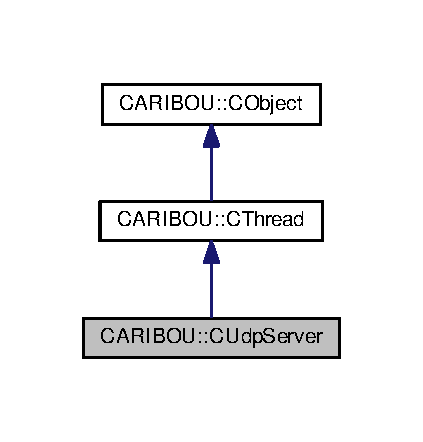
\includegraphics[width=203pt]{class_c_a_r_i_b_o_u_1_1_c_udp_server__inherit__graph}
\end{center}
\end{figure}


Collaboration diagram for C\+A\+R\+I\+B\+OU\+:\+:C\+Udp\+Server\+:\nopagebreak
\begin{figure}[H]
\begin{center}
\leavevmode
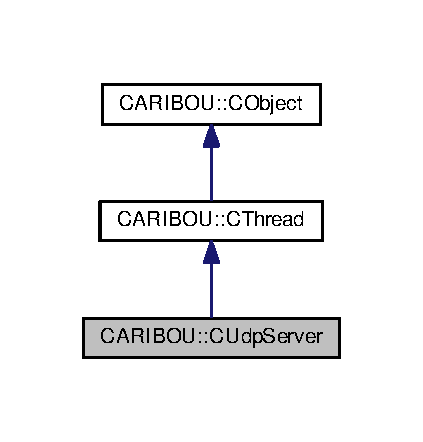
\includegraphics[width=203pt]{class_c_a_r_i_b_o_u_1_1_c_udp_server__coll__graph}
\end{center}
\end{figure}
\subsection*{Public Member Functions}
\begin{DoxyCompactItemize}
\item 
{\bf C\+Udp\+Server} (uint16\+\_\+t {\bf port}, uint32\+\_\+t {\bf interface}=I\+N\+A\+D\+D\+R\+\_\+\+A\+NY, int backlog=8, char $\ast${\bf name}=\char`\"{}tcpsrv\char`\"{}, uint32\+\_\+t stksize=512, uint16\+\_\+t {\bf priority}=0)
\begin{DoxyCompactList}\small\item\em A T\+CP server instance will set up a listener on each U\+DP port. \end{DoxyCompactList}\item 
virtual {\bf $\sim$\+C\+Udp\+Server} ()
\item 
uint32\+\_\+t {\bf interface} ()
\item 
uint16\+\_\+t {\bf port} ()
\item 
bool {\bf is\+Valid} ()
\begin{DoxyCompactList}\small\item\em Determin if the server is valid. \end{DoxyCompactList}\item 
void {\bf close} ()
\item 
virtual void {\bf run} ()
\end{DoxyCompactItemize}
\subsection*{Static Public Member Functions}
\begin{DoxyCompactItemize}
\item 
static {\bf C\+List}$<$ {\bf C\+Udp\+Server} $\ast$ $>$ \& {\bf servers} ()
\begin{DoxyCompactList}\small\item\em Return the list of servers. \end{DoxyCompactList}\item 
static {\bf C\+Udp\+Server} $\ast$ {\bf server} (uint16\+\_\+t {\bf port})
\begin{DoxyCompactList}\small\item\em Locate the T\+CP server instance servicing the port. \end{DoxyCompactList}\end{DoxyCompactItemize}
\subsection*{Protected Member Functions}
\begin{DoxyCompactItemize}
\item 
virtual void {\bf bind\+Error} (int rc, int err, const char $\ast$msg={\bf N\+U\+LL})
\item 
virtual void {\bf socket\+Error} (int rc, int err, const char $\ast$msg={\bf N\+U\+LL})
\item 
virtual void {\bf set\+Socket\+Options} ({\bf C\+Udp\+Socket} \&socket)
\item 
virtual bool {\bf fork} ({\bf C\+Udp\+Socket} \&socket)
\begin{DoxyCompactList}\small\item\em fork a session thread...this base class simply closes the socket \end{DoxyCompactList}\end{DoxyCompactItemize}
\subsection*{Additional Inherited Members}


\subsection{Detailed Description}


Definition at line 30 of file cudpserver.\+h.



\subsection{Constructor \& Destructor Documentation}
\index{C\+A\+R\+I\+B\+O\+U\+::\+C\+Udp\+Server@{C\+A\+R\+I\+B\+O\+U\+::\+C\+Udp\+Server}!C\+Udp\+Server@{C\+Udp\+Server}}
\index{C\+Udp\+Server@{C\+Udp\+Server}!C\+A\+R\+I\+B\+O\+U\+::\+C\+Udp\+Server@{C\+A\+R\+I\+B\+O\+U\+::\+C\+Udp\+Server}}
\subsubsection[{C\+Udp\+Server(uint16\+\_\+t port, uint32\+\_\+t interface=\+I\+N\+A\+D\+D\+R\+\_\+\+A\+N\+Y, int backlog=8, char $\ast$name=""tcpsrv"", uint32\+\_\+t stksize=512, uint16\+\_\+t priority=0)}]{\setlength{\rightskip}{0pt plus 5cm}C\+A\+R\+I\+B\+O\+U\+::\+C\+Udp\+Server\+::\+C\+Udp\+Server (
\begin{DoxyParamCaption}
\item[{uint16\+\_\+t}]{port, }
\item[{uint32\+\_\+t}]{interface = {\ttfamily INADDR\+\_\+ANY}, }
\item[{int}]{backlog = {\ttfamily 8}, }
\item[{char $\ast$}]{name = {\ttfamily \char`\"{}tcpsrv\char`\"{}}, }
\item[{uint32\+\_\+t}]{stksize = {\ttfamily 512}, }
\item[{uint16\+\_\+t}]{priority = {\ttfamily 0}}
\end{DoxyParamCaption}
)}\label{class_c_a_r_i_b_o_u_1_1_c_udp_server_a70e719d768ac1c0d39fcb72442d0945f}


A T\+CP server instance will set up a listener on each U\+DP port. 



Definition at line 28 of file cudpserver.\+cpp.

\index{C\+A\+R\+I\+B\+O\+U\+::\+C\+Udp\+Server@{C\+A\+R\+I\+B\+O\+U\+::\+C\+Udp\+Server}!````~C\+Udp\+Server@{$\sim$\+C\+Udp\+Server}}
\index{````~C\+Udp\+Server@{$\sim$\+C\+Udp\+Server}!C\+A\+R\+I\+B\+O\+U\+::\+C\+Udp\+Server@{C\+A\+R\+I\+B\+O\+U\+::\+C\+Udp\+Server}}
\subsubsection[{$\sim$\+C\+Udp\+Server()}]{\setlength{\rightskip}{0pt plus 5cm}C\+A\+R\+I\+B\+O\+U\+::\+C\+Udp\+Server\+::$\sim$\+C\+Udp\+Server (
\begin{DoxyParamCaption}
{}
\end{DoxyParamCaption}
)\hspace{0.3cm}{\ttfamily [virtual]}}\label{class_c_a_r_i_b_o_u_1_1_c_udp_server_a6b081be56772f33d59d8a6cf4508ae88}


Definition at line 40 of file cudpserver.\+cpp.



\subsection{Member Function Documentation}
\index{C\+A\+R\+I\+B\+O\+U\+::\+C\+Udp\+Server@{C\+A\+R\+I\+B\+O\+U\+::\+C\+Udp\+Server}!bind\+Error@{bind\+Error}}
\index{bind\+Error@{bind\+Error}!C\+A\+R\+I\+B\+O\+U\+::\+C\+Udp\+Server@{C\+A\+R\+I\+B\+O\+U\+::\+C\+Udp\+Server}}
\subsubsection[{bind\+Error(int rc, int err, const char $\ast$msg=\+N\+U\+L\+L)}]{\setlength{\rightskip}{0pt plus 5cm}virtual void C\+A\+R\+I\+B\+O\+U\+::\+C\+Udp\+Server\+::bind\+Error (
\begin{DoxyParamCaption}
\item[{int}]{rc, }
\item[{int}]{err, }
\item[{const char $\ast$}]{msg = {\ttfamily {\bf N\+U\+LL}}}
\end{DoxyParamCaption}
)\hspace{0.3cm}{\ttfamily [inline]}, {\ttfamily [protected]}, {\ttfamily [virtual]}}\label{class_c_a_r_i_b_o_u_1_1_c_udp_server_a466894ea00a2e8883e14f8c14db4edb8}


Definition at line 45 of file cudpserver.\+h.

\index{C\+A\+R\+I\+B\+O\+U\+::\+C\+Udp\+Server@{C\+A\+R\+I\+B\+O\+U\+::\+C\+Udp\+Server}!close@{close}}
\index{close@{close}!C\+A\+R\+I\+B\+O\+U\+::\+C\+Udp\+Server@{C\+A\+R\+I\+B\+O\+U\+::\+C\+Udp\+Server}}
\subsubsection[{close()}]{\setlength{\rightskip}{0pt plus 5cm}void C\+A\+R\+I\+B\+O\+U\+::\+C\+Udp\+Server\+::close (
\begin{DoxyParamCaption}
{}
\end{DoxyParamCaption}
)}\label{class_c_a_r_i_b_o_u_1_1_c_udp_server_a3785f5751c35d38d0a26d5c52f6f1181}


Definition at line 59 of file cudpserver.\+cpp.

\index{C\+A\+R\+I\+B\+O\+U\+::\+C\+Udp\+Server@{C\+A\+R\+I\+B\+O\+U\+::\+C\+Udp\+Server}!fork@{fork}}
\index{fork@{fork}!C\+A\+R\+I\+B\+O\+U\+::\+C\+Udp\+Server@{C\+A\+R\+I\+B\+O\+U\+::\+C\+Udp\+Server}}
\subsubsection[{fork(\+C\+Udp\+Socket \&socket)}]{\setlength{\rightskip}{0pt plus 5cm}bool C\+A\+R\+I\+B\+O\+U\+::\+C\+Udp\+Server\+::fork (
\begin{DoxyParamCaption}
\item[{{\bf C\+Udp\+Socket} \&}]{socket}
\end{DoxyParamCaption}
)\hspace{0.3cm}{\ttfamily [protected]}, {\ttfamily [virtual]}}\label{class_c_a_r_i_b_o_u_1_1_c_udp_server_a0e6ea080d268a8c0c733e549a44bc345}


fork a session thread...this base class simply closes the socket 



Definition at line 126 of file cudpserver.\+cpp.

\index{C\+A\+R\+I\+B\+O\+U\+::\+C\+Udp\+Server@{C\+A\+R\+I\+B\+O\+U\+::\+C\+Udp\+Server}!interface@{interface}}
\index{interface@{interface}!C\+A\+R\+I\+B\+O\+U\+::\+C\+Udp\+Server@{C\+A\+R\+I\+B\+O\+U\+::\+C\+Udp\+Server}}
\subsubsection[{interface()}]{\setlength{\rightskip}{0pt plus 5cm}uint32\+\_\+t C\+A\+R\+I\+B\+O\+U\+::\+C\+Udp\+Server\+::interface (
\begin{DoxyParamCaption}
{}
\end{DoxyParamCaption}
)}\label{class_c_a_r_i_b_o_u_1_1_c_udp_server_ac88a24ad60d2c439eee0be718096f734}
\begin{DoxyReturn}{Returns}
The address of the interface 
\end{DoxyReturn}


Definition at line 90 of file cudpserver.\+cpp.

\index{C\+A\+R\+I\+B\+O\+U\+::\+C\+Udp\+Server@{C\+A\+R\+I\+B\+O\+U\+::\+C\+Udp\+Server}!is\+Valid@{is\+Valid}}
\index{is\+Valid@{is\+Valid}!C\+A\+R\+I\+B\+O\+U\+::\+C\+Udp\+Server@{C\+A\+R\+I\+B\+O\+U\+::\+C\+Udp\+Server}}
\subsubsection[{is\+Valid()}]{\setlength{\rightskip}{0pt plus 5cm}bool C\+A\+R\+I\+B\+O\+U\+::\+C\+Udp\+Server\+::is\+Valid (
\begin{DoxyParamCaption}
{}
\end{DoxyParamCaption}
)}\label{class_c_a_r_i_b_o_u_1_1_c_udp_server_a6a2c3b39e105726a5bd1cdbe8da9d705}


Determin if the server is valid. 



Definition at line 54 of file cudpserver.\+cpp.

\index{C\+A\+R\+I\+B\+O\+U\+::\+C\+Udp\+Server@{C\+A\+R\+I\+B\+O\+U\+::\+C\+Udp\+Server}!port@{port}}
\index{port@{port}!C\+A\+R\+I\+B\+O\+U\+::\+C\+Udp\+Server@{C\+A\+R\+I\+B\+O\+U\+::\+C\+Udp\+Server}}
\subsubsection[{port()}]{\setlength{\rightskip}{0pt plus 5cm}uint16\+\_\+t C\+A\+R\+I\+B\+O\+U\+::\+C\+Udp\+Server\+::port (
\begin{DoxyParamCaption}
{}
\end{DoxyParamCaption}
)}\label{class_c_a_r_i_b_o_u_1_1_c_udp_server_a15599b94c1de09d3620dea93bd496bed}
\begin{DoxyReturn}{Returns}
The port of the interface 
\end{DoxyReturn}


Definition at line 106 of file cudpserver.\+cpp.

\index{C\+A\+R\+I\+B\+O\+U\+::\+C\+Udp\+Server@{C\+A\+R\+I\+B\+O\+U\+::\+C\+Udp\+Server}!run@{run}}
\index{run@{run}!C\+A\+R\+I\+B\+O\+U\+::\+C\+Udp\+Server@{C\+A\+R\+I\+B\+O\+U\+::\+C\+Udp\+Server}}
\subsubsection[{run()}]{\setlength{\rightskip}{0pt plus 5cm}void C\+A\+R\+I\+B\+O\+U\+::\+C\+Udp\+Server\+::run (
\begin{DoxyParamCaption}
{}
\end{DoxyParamCaption}
)\hspace{0.3cm}{\ttfamily [virtual]}}\label{class_c_a_r_i_b_o_u_1_1_c_udp_server_a57eefe6dd725771c49ca33eb332fd291}


Implements {\bf C\+A\+R\+I\+B\+O\+U\+::\+C\+Thread} \doxyref{}{p.}{class_c_a_r_i_b_o_u_1_1_c_thread_a087ae48a158aca84892aea7f9ed16711}.



Definition at line 131 of file cudpserver.\+cpp.

\index{C\+A\+R\+I\+B\+O\+U\+::\+C\+Udp\+Server@{C\+A\+R\+I\+B\+O\+U\+::\+C\+Udp\+Server}!server@{server}}
\index{server@{server}!C\+A\+R\+I\+B\+O\+U\+::\+C\+Udp\+Server@{C\+A\+R\+I\+B\+O\+U\+::\+C\+Udp\+Server}}
\subsubsection[{server(uint16\+\_\+t port)}]{\setlength{\rightskip}{0pt plus 5cm}{\bf C\+Udp\+Server} $\ast$ C\+A\+R\+I\+B\+O\+U\+::\+C\+Udp\+Server\+::server (
\begin{DoxyParamCaption}
\item[{uint16\+\_\+t}]{port}
\end{DoxyParamCaption}
)\hspace{0.3cm}{\ttfamily [static]}}\label{class_c_a_r_i_b_o_u_1_1_c_udp_server_ab90075095409468ef9193cee161906a9}


Locate the T\+CP server instance servicing the port. 


\begin{DoxyParams}{Parameters}
{\em port} & The port to search for. \\
\hline
\end{DoxyParams}
\begin{DoxyReturn}{Returns}
Return the server instance or N\+U\+LL. 
\end{DoxyReturn}


Definition at line 70 of file cudpserver.\+cpp.

\index{C\+A\+R\+I\+B\+O\+U\+::\+C\+Udp\+Server@{C\+A\+R\+I\+B\+O\+U\+::\+C\+Udp\+Server}!servers@{servers}}
\index{servers@{servers}!C\+A\+R\+I\+B\+O\+U\+::\+C\+Udp\+Server@{C\+A\+R\+I\+B\+O\+U\+::\+C\+Udp\+Server}}
\subsubsection[{servers()}]{\setlength{\rightskip}{0pt plus 5cm}{\bf C\+List}$<$ {\bf C\+Udp\+Server} $\ast$ $>$ \& C\+A\+R\+I\+B\+O\+U\+::\+C\+Udp\+Server\+::servers (
\begin{DoxyParamCaption}
{}
\end{DoxyParamCaption}
)\hspace{0.3cm}{\ttfamily [static]}}\label{class_c_a_r_i_b_o_u_1_1_c_udp_server_ac6fba07d346779e9ac2fbfcae131d76b}


Return the list of servers. 



Definition at line 48 of file cudpserver.\+cpp.

\index{C\+A\+R\+I\+B\+O\+U\+::\+C\+Udp\+Server@{C\+A\+R\+I\+B\+O\+U\+::\+C\+Udp\+Server}!set\+Socket\+Options@{set\+Socket\+Options}}
\index{set\+Socket\+Options@{set\+Socket\+Options}!C\+A\+R\+I\+B\+O\+U\+::\+C\+Udp\+Server@{C\+A\+R\+I\+B\+O\+U\+::\+C\+Udp\+Server}}
\subsubsection[{set\+Socket\+Options(\+C\+Udp\+Socket \&socket)}]{\setlength{\rightskip}{0pt plus 5cm}void C\+A\+R\+I\+B\+O\+U\+::\+C\+Udp\+Server\+::set\+Socket\+Options (
\begin{DoxyParamCaption}
\item[{{\bf C\+Udp\+Socket} \&}]{socket}
\end{DoxyParamCaption}
)\hspace{0.3cm}{\ttfamily [protected]}, {\ttfamily [virtual]}}\label{class_c_a_r_i_b_o_u_1_1_c_udp_server_aa3939f66bd17dd5017c36489c7364957}


Definition at line 121 of file cudpserver.\+cpp.

\index{C\+A\+R\+I\+B\+O\+U\+::\+C\+Udp\+Server@{C\+A\+R\+I\+B\+O\+U\+::\+C\+Udp\+Server}!socket\+Error@{socket\+Error}}
\index{socket\+Error@{socket\+Error}!C\+A\+R\+I\+B\+O\+U\+::\+C\+Udp\+Server@{C\+A\+R\+I\+B\+O\+U\+::\+C\+Udp\+Server}}
\subsubsection[{socket\+Error(int rc, int err, const char $\ast$msg=\+N\+U\+L\+L)}]{\setlength{\rightskip}{0pt plus 5cm}virtual void C\+A\+R\+I\+B\+O\+U\+::\+C\+Udp\+Server\+::socket\+Error (
\begin{DoxyParamCaption}
\item[{int}]{rc, }
\item[{int}]{err, }
\item[{const char $\ast$}]{msg = {\ttfamily {\bf N\+U\+LL}}}
\end{DoxyParamCaption}
)\hspace{0.3cm}{\ttfamily [inline]}, {\ttfamily [protected]}, {\ttfamily [virtual]}}\label{class_c_a_r_i_b_o_u_1_1_c_udp_server_a2350a22d56d3fbf09f5e7812fe54445a}


Definition at line 46 of file cudpserver.\+h.



The documentation for this class was generated from the following files\+:\begin{DoxyCompactItemize}
\item 
include/caribou++/{\bf cudpserver.\+h}\item 
src/{\bf cudpserver.\+cpp}\end{DoxyCompactItemize}

\section{C\+A\+R\+I\+B\+OU\+:\+:C\+Udp\+Session Class Reference}
\label{class_c_a_r_i_b_o_u_1_1_c_udp_session}\index{C\+A\+R\+I\+B\+O\+U\+::\+C\+Udp\+Session@{C\+A\+R\+I\+B\+O\+U\+::\+C\+Udp\+Session}}


{\ttfamily \#include $<$cudpsession.\+h$>$}



Inheritance diagram for C\+A\+R\+I\+B\+OU\+:\+:C\+Udp\+Session\+:\nopagebreak
\begin{figure}[H]
\begin{center}
\leavevmode
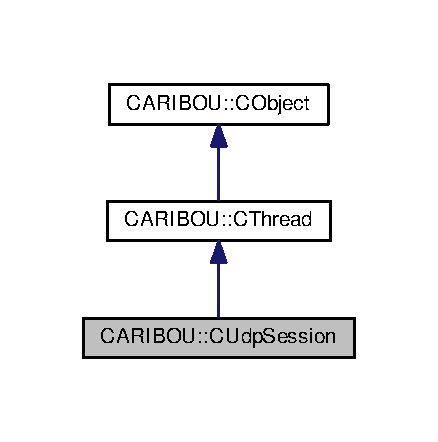
\includegraphics[width=210pt]{class_c_a_r_i_b_o_u_1_1_c_udp_session__inherit__graph}
\end{center}
\end{figure}


Collaboration diagram for C\+A\+R\+I\+B\+OU\+:\+:C\+Udp\+Session\+:\nopagebreak
\begin{figure}[H]
\begin{center}
\leavevmode
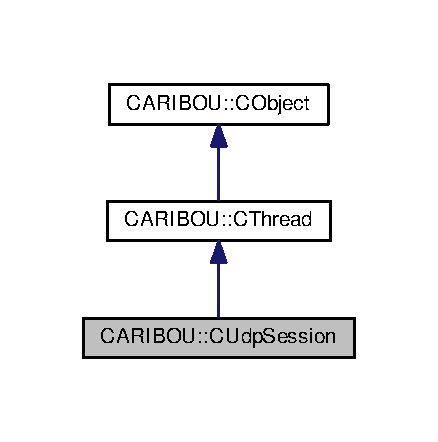
\includegraphics[width=210pt]{class_c_a_r_i_b_o_u_1_1_c_udp_session__coll__graph}
\end{center}
\end{figure}
\subsection*{Public Member Functions}
\begin{DoxyCompactItemize}
\item 
{\bf C\+Udp\+Session} (const char $\ast${\bf name}=\char`\"{}tcp\char`\"{}, uint16\+\_\+t stksize=512, uint16\+\_\+t {\bf priority}=0)
\item 
virtual {\bf $\sim$\+C\+Udp\+Session} ()
\item 
virtual void {\bf append\+Socket} (int {\bf socket})
\item 
int {\bf socket\+Count} ()
\end{DoxyCompactItemize}
\subsection*{Protected Member Functions}
\begin{DoxyCompactItemize}
\item 
virtual void {\bf run} ()
\item 
{\bf C\+A\+R\+I\+B\+O\+U\+::\+C\+Udp\+Socket} \& {\bf next\+Socket} ()
\begin{DoxyCompactList}\small\item\em Get the next socket in the queue ala round-\/robin. \end{DoxyCompactList}\item 
{\bf C\+A\+R\+I\+B\+O\+U\+::\+C\+Udp\+Socket} \& {\bf take\+Socket} ()
\item 
void {\bf dequeue\+Socket} ()
\begin{DoxyCompactList}\small\item\em Dequeue the current socket. \end{DoxyCompactList}\item 
void {\bf close\+Socket} ()
\item 
{\bf C\+A\+R\+I\+B\+O\+U\+::\+C\+Udp\+Socket} \& {\bf socket} ()
\item 
{\bf C\+A\+R\+I\+B\+O\+U\+::\+C\+List}$<$ int $>$ \& {\bf socket\+Queue} ()
\item 
{\bf C\+A\+R\+I\+B\+O\+U\+::\+C\+Udp\+Socket} \& {\bf set\+Socket} (int {\bf socket})
\end{DoxyCompactItemize}
\subsection*{Additional Inherited Members}


\subsection{Detailed Description}


Definition at line 28 of file cudpsession.\+h.



\subsection{Constructor \& Destructor Documentation}
\index{C\+A\+R\+I\+B\+O\+U\+::\+C\+Udp\+Session@{C\+A\+R\+I\+B\+O\+U\+::\+C\+Udp\+Session}!C\+Udp\+Session@{C\+Udp\+Session}}
\index{C\+Udp\+Session@{C\+Udp\+Session}!C\+A\+R\+I\+B\+O\+U\+::\+C\+Udp\+Session@{C\+A\+R\+I\+B\+O\+U\+::\+C\+Udp\+Session}}
\subsubsection[{C\+Udp\+Session(const char $\ast$name=""tcp"", uint16\+\_\+t stksize=512, uint16\+\_\+t priority=0)}]{\setlength{\rightskip}{0pt plus 5cm}C\+A\+R\+I\+B\+O\+U\+::\+C\+Udp\+Session\+::\+C\+Udp\+Session (
\begin{DoxyParamCaption}
\item[{const char $\ast$}]{name = {\ttfamily \char`\"{}tcp\char`\"{}}, }
\item[{uint16\+\_\+t}]{stksize = {\ttfamily 512}, }
\item[{uint16\+\_\+t}]{priority = {\ttfamily 0}}
\end{DoxyParamCaption}
)}\label{class_c_a_r_i_b_o_u_1_1_c_udp_session_ab83fe760c4c3f346ca3a97769a4ad2ad}


Definition at line 24 of file cudpsession.\+cpp.

\index{C\+A\+R\+I\+B\+O\+U\+::\+C\+Udp\+Session@{C\+A\+R\+I\+B\+O\+U\+::\+C\+Udp\+Session}!````~C\+Udp\+Session@{$\sim$\+C\+Udp\+Session}}
\index{````~C\+Udp\+Session@{$\sim$\+C\+Udp\+Session}!C\+A\+R\+I\+B\+O\+U\+::\+C\+Udp\+Session@{C\+A\+R\+I\+B\+O\+U\+::\+C\+Udp\+Session}}
\subsubsection[{$\sim$\+C\+Udp\+Session()}]{\setlength{\rightskip}{0pt plus 5cm}C\+A\+R\+I\+B\+O\+U\+::\+C\+Udp\+Session\+::$\sim$\+C\+Udp\+Session (
\begin{DoxyParamCaption}
{}
\end{DoxyParamCaption}
)\hspace{0.3cm}{\ttfamily [virtual]}}\label{class_c_a_r_i_b_o_u_1_1_c_udp_session_ac845d16856a0ec1bf2de74f5efe704e6}


Definition at line 29 of file cudpsession.\+cpp.



\subsection{Member Function Documentation}
\index{C\+A\+R\+I\+B\+O\+U\+::\+C\+Udp\+Session@{C\+A\+R\+I\+B\+O\+U\+::\+C\+Udp\+Session}!append\+Socket@{append\+Socket}}
\index{append\+Socket@{append\+Socket}!C\+A\+R\+I\+B\+O\+U\+::\+C\+Udp\+Session@{C\+A\+R\+I\+B\+O\+U\+::\+C\+Udp\+Session}}
\subsubsection[{append\+Socket(int socket)}]{\setlength{\rightskip}{0pt plus 5cm}void C\+A\+R\+I\+B\+O\+U\+::\+C\+Udp\+Session\+::append\+Socket (
\begin{DoxyParamCaption}
\item[{int}]{socket}
\end{DoxyParamCaption}
)\hspace{0.3cm}{\ttfamily [virtual]}}\label{class_c_a_r_i_b_o_u_1_1_c_udp_session_a029f484374789ab1272f13c6543b22dc}


Definition at line 49 of file cudpsession.\+cpp.

\index{C\+A\+R\+I\+B\+O\+U\+::\+C\+Udp\+Session@{C\+A\+R\+I\+B\+O\+U\+::\+C\+Udp\+Session}!close\+Socket@{close\+Socket}}
\index{close\+Socket@{close\+Socket}!C\+A\+R\+I\+B\+O\+U\+::\+C\+Udp\+Session@{C\+A\+R\+I\+B\+O\+U\+::\+C\+Udp\+Session}}
\subsubsection[{close\+Socket()}]{\setlength{\rightskip}{0pt plus 5cm}void C\+A\+R\+I\+B\+O\+U\+::\+C\+Udp\+Session\+::close\+Socket (
\begin{DoxyParamCaption}
{}
\end{DoxyParamCaption}
)\hspace{0.3cm}{\ttfamily [protected]}}\label{class_c_a_r_i_b_o_u_1_1_c_udp_session_ab81ee8d2a3b859fe266ca37fe061cc41}


Definition at line 102 of file cudpsession.\+cpp.

\index{C\+A\+R\+I\+B\+O\+U\+::\+C\+Udp\+Session@{C\+A\+R\+I\+B\+O\+U\+::\+C\+Udp\+Session}!dequeue\+Socket@{dequeue\+Socket}}
\index{dequeue\+Socket@{dequeue\+Socket}!C\+A\+R\+I\+B\+O\+U\+::\+C\+Udp\+Session@{C\+A\+R\+I\+B\+O\+U\+::\+C\+Udp\+Session}}
\subsubsection[{dequeue\+Socket()}]{\setlength{\rightskip}{0pt plus 5cm}void C\+A\+R\+I\+B\+O\+U\+::\+C\+Udp\+Session\+::dequeue\+Socket (
\begin{DoxyParamCaption}
{}
\end{DoxyParamCaption}
)\hspace{0.3cm}{\ttfamily [protected]}}\label{class_c_a_r_i_b_o_u_1_1_c_udp_session_a47cbe09f9116ec3fd8caa301aab9bdb8}


Dequeue the current socket. 



Definition at line 92 of file cudpsession.\+cpp.

\index{C\+A\+R\+I\+B\+O\+U\+::\+C\+Udp\+Session@{C\+A\+R\+I\+B\+O\+U\+::\+C\+Udp\+Session}!next\+Socket@{next\+Socket}}
\index{next\+Socket@{next\+Socket}!C\+A\+R\+I\+B\+O\+U\+::\+C\+Udp\+Session@{C\+A\+R\+I\+B\+O\+U\+::\+C\+Udp\+Session}}
\subsubsection[{next\+Socket()}]{\setlength{\rightskip}{0pt plus 5cm}{\bf C\+A\+R\+I\+B\+O\+U\+::\+C\+Udp\+Socket} \& C\+A\+R\+I\+B\+O\+U\+::\+C\+Udp\+Session\+::next\+Socket (
\begin{DoxyParamCaption}
{}
\end{DoxyParamCaption}
)\hspace{0.3cm}{\ttfamily [protected]}}\label{class_c_a_r_i_b_o_u_1_1_c_udp_session_a2d4c26aaabfca4a8bfcecd295ca48ac2}


Get the next socket in the queue ala round-\/robin. 



Definition at line 57 of file cudpsession.\+cpp.

\index{C\+A\+R\+I\+B\+O\+U\+::\+C\+Udp\+Session@{C\+A\+R\+I\+B\+O\+U\+::\+C\+Udp\+Session}!run@{run}}
\index{run@{run}!C\+A\+R\+I\+B\+O\+U\+::\+C\+Udp\+Session@{C\+A\+R\+I\+B\+O\+U\+::\+C\+Udp\+Session}}
\subsubsection[{run()}]{\setlength{\rightskip}{0pt plus 5cm}void C\+A\+R\+I\+B\+O\+U\+::\+C\+Udp\+Session\+::run (
\begin{DoxyParamCaption}
{}
\end{DoxyParamCaption}
)\hspace{0.3cm}{\ttfamily [protected]}, {\ttfamily [virtual]}}\label{class_c_a_r_i_b_o_u_1_1_c_udp_session_a59a2d243c8d8ad6dc08ce93b9b6fb712}


Implements {\bf C\+A\+R\+I\+B\+O\+U\+::\+C\+Thread} \doxyref{}{p.}{class_c_a_r_i_b_o_u_1_1_c_thread_a087ae48a158aca84892aea7f9ed16711}.



Definition at line 122 of file cudpsession.\+cpp.

\index{C\+A\+R\+I\+B\+O\+U\+::\+C\+Udp\+Session@{C\+A\+R\+I\+B\+O\+U\+::\+C\+Udp\+Session}!set\+Socket@{set\+Socket}}
\index{set\+Socket@{set\+Socket}!C\+A\+R\+I\+B\+O\+U\+::\+C\+Udp\+Session@{C\+A\+R\+I\+B\+O\+U\+::\+C\+Udp\+Session}}
\subsubsection[{set\+Socket(int socket)}]{\setlength{\rightskip}{0pt plus 5cm}{\bf C\+A\+R\+I\+B\+O\+U\+::\+C\+Udp\+Socket} \& C\+A\+R\+I\+B\+O\+U\+::\+C\+Udp\+Session\+::set\+Socket (
\begin{DoxyParamCaption}
\item[{int}]{socket}
\end{DoxyParamCaption}
)\hspace{0.3cm}{\ttfamily [protected]}}\label{class_c_a_r_i_b_o_u_1_1_c_udp_session_a60a0870513bb433ef99709d31183ee87}


Definition at line 115 of file cudpsession.\+cpp.

\index{C\+A\+R\+I\+B\+O\+U\+::\+C\+Udp\+Session@{C\+A\+R\+I\+B\+O\+U\+::\+C\+Udp\+Session}!socket@{socket}}
\index{socket@{socket}!C\+A\+R\+I\+B\+O\+U\+::\+C\+Udp\+Session@{C\+A\+R\+I\+B\+O\+U\+::\+C\+Udp\+Session}}
\subsubsection[{socket()}]{\setlength{\rightskip}{0pt plus 5cm}{\bf C\+A\+R\+I\+B\+O\+U\+::\+C\+Udp\+Socket} \& C\+A\+R\+I\+B\+O\+U\+::\+C\+Udp\+Session\+::socket (
\begin{DoxyParamCaption}
{}
\end{DoxyParamCaption}
)\hspace{0.3cm}{\ttfamily [protected]}}\label{class_c_a_r_i_b_o_u_1_1_c_udp_session_a62420e2974eea6590f36f27df724af7a}


Definition at line 110 of file cudpsession.\+cpp.

\index{C\+A\+R\+I\+B\+O\+U\+::\+C\+Udp\+Session@{C\+A\+R\+I\+B\+O\+U\+::\+C\+Udp\+Session}!socket\+Count@{socket\+Count}}
\index{socket\+Count@{socket\+Count}!C\+A\+R\+I\+B\+O\+U\+::\+C\+Udp\+Session@{C\+A\+R\+I\+B\+O\+U\+::\+C\+Udp\+Session}}
\subsubsection[{socket\+Count()}]{\setlength{\rightskip}{0pt plus 5cm}int C\+A\+R\+I\+B\+O\+U\+::\+C\+Udp\+Session\+::socket\+Count (
\begin{DoxyParamCaption}
{}
\end{DoxyParamCaption}
)}\label{class_c_a_r_i_b_o_u_1_1_c_udp_session_a7d3ee6621fd222d8cb6a97eb39ead4a3}


Definition at line 40 of file cudpsession.\+cpp.

\index{C\+A\+R\+I\+B\+O\+U\+::\+C\+Udp\+Session@{C\+A\+R\+I\+B\+O\+U\+::\+C\+Udp\+Session}!socket\+Queue@{socket\+Queue}}
\index{socket\+Queue@{socket\+Queue}!C\+A\+R\+I\+B\+O\+U\+::\+C\+Udp\+Session@{C\+A\+R\+I\+B\+O\+U\+::\+C\+Udp\+Session}}
\subsubsection[{socket\+Queue()}]{\setlength{\rightskip}{0pt plus 5cm}{\bf C\+A\+R\+I\+B\+O\+U\+::\+C\+List}$<$ int $>$ \& C\+A\+R\+I\+B\+O\+U\+::\+C\+Udp\+Session\+::socket\+Queue (
\begin{DoxyParamCaption}
{}
\end{DoxyParamCaption}
)\hspace{0.3cm}{\ttfamily [protected]}}\label{class_c_a_r_i_b_o_u_1_1_c_udp_session_a923562aaf1dd0e7de6acdd89e3ecb2b7}


Definition at line 35 of file cudpsession.\+cpp.

\index{C\+A\+R\+I\+B\+O\+U\+::\+C\+Udp\+Session@{C\+A\+R\+I\+B\+O\+U\+::\+C\+Udp\+Session}!take\+Socket@{take\+Socket}}
\index{take\+Socket@{take\+Socket}!C\+A\+R\+I\+B\+O\+U\+::\+C\+Udp\+Session@{C\+A\+R\+I\+B\+O\+U\+::\+C\+Udp\+Session}}
\subsubsection[{take\+Socket()}]{\setlength{\rightskip}{0pt plus 5cm}{\bf C\+A\+R\+I\+B\+O\+U\+::\+C\+Udp\+Socket} \& C\+A\+R\+I\+B\+O\+U\+::\+C\+Udp\+Session\+::take\+Socket (
\begin{DoxyParamCaption}
{}
\end{DoxyParamCaption}
)\hspace{0.3cm}{\ttfamily [protected]}}\label{class_c_a_r_i_b_o_u_1_1_c_udp_session_abb023235799abfaaf0abf5187b3acb9c}


Definition at line 80 of file cudpsession.\+cpp.



The documentation for this class was generated from the following files\+:\begin{DoxyCompactItemize}
\item 
include/caribou++/{\bf cudpsession.\+h}\item 
src/{\bf cudpsession.\+cpp}\end{DoxyCompactItemize}

\section{C\-A\-R\-I\-B\-O\-U\-:\-:C\-Udp\-Socket Class Reference}
\label{class_c_a_r_i_b_o_u_1_1_c_udp_socket}\index{C\-A\-R\-I\-B\-O\-U\-::\-C\-Udp\-Socket@{C\-A\-R\-I\-B\-O\-U\-::\-C\-Udp\-Socket}}


The \doxyref{C\-Udp\-Socket}{p.}{class_c_a_r_i_b_o_u_1_1_c_udp_socket} class provides a T\-C\-P socket.  




{\ttfamily \#include $<$cudpsocket.\-h$>$}



Inheritance diagram for C\-A\-R\-I\-B\-O\-U\-:\-:C\-Udp\-Socket\-:\nopagebreak
\begin{figure}[H]
\begin{center}
\leavevmode
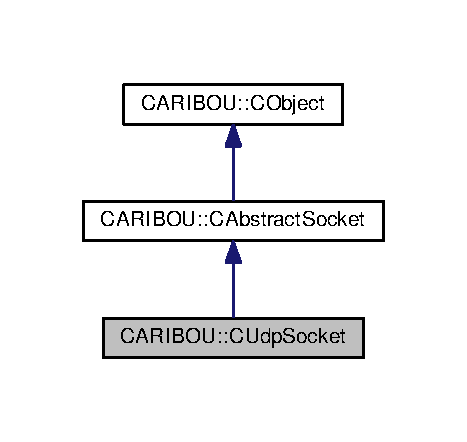
\includegraphics[width=224pt]{class_c_a_r_i_b_o_u_1_1_c_udp_socket__inherit__graph}
\end{center}
\end{figure}


Collaboration diagram for C\-A\-R\-I\-B\-O\-U\-:\-:C\-Udp\-Socket\-:\nopagebreak
\begin{figure}[H]
\begin{center}
\leavevmode
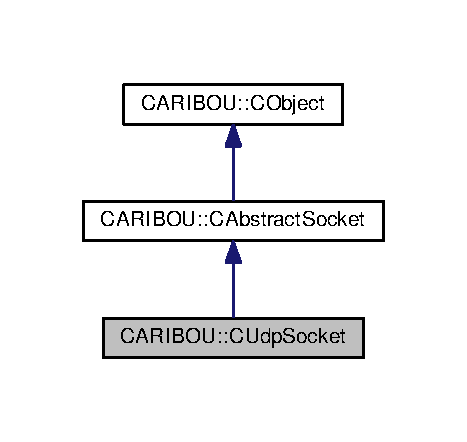
\includegraphics[width=224pt]{class_c_a_r_i_b_o_u_1_1_c_udp_socket__coll__graph}
\end{center}
\end{figure}
\subsection*{Public Member Functions}
\begin{DoxyCompactItemize}
\item 
{\bf C\-Udp\-Socket} ()
\item 
{\bf C\-Udp\-Socket} (int {\bf socket})
\item 
{\bf C\-Udp\-Socket} (int domain, int type, int protocol)
\item 
{\bf C\-Udp\-Socket} (const {\bf C\-Udp\-Socket} \&other)
\item 
virtual {\bf $\sim$\-C\-Udp\-Socket} ()
\item 
int {\bf send} (char $\ast$buf, int len, int flags=0)
\begin{DoxyCompactList}\small\item\em \doxyref{C\-Abstract\-Socket}{p.}{class_c_a_r_i_b_o_u_1_1_c_abstract_socket} overrides. \end{DoxyCompactList}\item 
int {\bf send} ({\bf C\-A\-R\-I\-B\-O\-U\-::\-C\-Byte\-Array} \&buf, int flags=0)
\begin{DoxyCompactList}\small\item\em Sends bytes. \end{DoxyCompactList}\item 
{\bf C\-Udp\-Socket} \& {\bf operator=} (const {\bf C\-Udp\-Socket} \&other)
\item 
bool {\bf operator==} ({\bf C\-Udp\-Socket} \&other)
\end{DoxyCompactItemize}
\subsection*{Additional Inherited Members}


\subsection{Detailed Description}
The \doxyref{C\-Udp\-Socket}{p.}{class_c_a_r_i_b_o_u_1_1_c_udp_socket} class provides a T\-C\-P socket. 

T\-C\-P (Transmission Control Protocol) is a reliable, stream-\/oriented, connection-\/oriented transport protocol. It is especially well suited for continuous transmission of data. 

Definition at line 31 of file cudpsocket.\-h.



\subsection{Constructor \& Destructor Documentation}
\index{C\-A\-R\-I\-B\-O\-U\-::\-C\-Udp\-Socket@{C\-A\-R\-I\-B\-O\-U\-::\-C\-Udp\-Socket}!C\-Udp\-Socket@{C\-Udp\-Socket}}
\index{C\-Udp\-Socket@{C\-Udp\-Socket}!CARIBOU::CUdpSocket@{C\-A\-R\-I\-B\-O\-U\-::\-C\-Udp\-Socket}}
\subsubsection[{C\-Udp\-Socket}]{\setlength{\rightskip}{0pt plus 5cm}C\-A\-R\-I\-B\-O\-U\-::\-C\-Udp\-Socket\-::\-C\-Udp\-Socket (
\begin{DoxyParamCaption}
{}
\end{DoxyParamCaption}
)}\label{class_c_a_r_i_b_o_u_1_1_c_udp_socket_adae4a0ff5d598f461c6f5436acef306b}


Definition at line 29 of file cudpsocket.\-cpp.

\index{C\-A\-R\-I\-B\-O\-U\-::\-C\-Udp\-Socket@{C\-A\-R\-I\-B\-O\-U\-::\-C\-Udp\-Socket}!C\-Udp\-Socket@{C\-Udp\-Socket}}
\index{C\-Udp\-Socket@{C\-Udp\-Socket}!CARIBOU::CUdpSocket@{C\-A\-R\-I\-B\-O\-U\-::\-C\-Udp\-Socket}}
\subsubsection[{C\-Udp\-Socket}]{\setlength{\rightskip}{0pt plus 5cm}C\-A\-R\-I\-B\-O\-U\-::\-C\-Udp\-Socket\-::\-C\-Udp\-Socket (
\begin{DoxyParamCaption}
\item[{int}]{socket}
\end{DoxyParamCaption}
)}\label{class_c_a_r_i_b_o_u_1_1_c_udp_socket_a76f99d16dc7de81521dee820611e4067}


Definition at line 34 of file cudpsocket.\-cpp.

\index{C\-A\-R\-I\-B\-O\-U\-::\-C\-Udp\-Socket@{C\-A\-R\-I\-B\-O\-U\-::\-C\-Udp\-Socket}!C\-Udp\-Socket@{C\-Udp\-Socket}}
\index{C\-Udp\-Socket@{C\-Udp\-Socket}!CARIBOU::CUdpSocket@{C\-A\-R\-I\-B\-O\-U\-::\-C\-Udp\-Socket}}
\subsubsection[{C\-Udp\-Socket}]{\setlength{\rightskip}{0pt plus 5cm}C\-A\-R\-I\-B\-O\-U\-::\-C\-Udp\-Socket\-::\-C\-Udp\-Socket (
\begin{DoxyParamCaption}
\item[{int}]{domain, }
\item[{int}]{type, }
\item[{int}]{protocol}
\end{DoxyParamCaption}
)}\label{class_c_a_r_i_b_o_u_1_1_c_udp_socket_a4611a6420deb80893a57ab4e5381bd92}


Definition at line 39 of file cudpsocket.\-cpp.

\index{C\-A\-R\-I\-B\-O\-U\-::\-C\-Udp\-Socket@{C\-A\-R\-I\-B\-O\-U\-::\-C\-Udp\-Socket}!C\-Udp\-Socket@{C\-Udp\-Socket}}
\index{C\-Udp\-Socket@{C\-Udp\-Socket}!CARIBOU::CUdpSocket@{C\-A\-R\-I\-B\-O\-U\-::\-C\-Udp\-Socket}}
\subsubsection[{C\-Udp\-Socket}]{\setlength{\rightskip}{0pt plus 5cm}C\-A\-R\-I\-B\-O\-U\-::\-C\-Udp\-Socket\-::\-C\-Udp\-Socket (
\begin{DoxyParamCaption}
\item[{const {\bf C\-Udp\-Socket} \&}]{other}
\end{DoxyParamCaption}
)}\label{class_c_a_r_i_b_o_u_1_1_c_udp_socket_a2a0e1de617022b300a0ed2d647e6d06a}


Definition at line 44 of file cudpsocket.\-cpp.

\index{C\-A\-R\-I\-B\-O\-U\-::\-C\-Udp\-Socket@{C\-A\-R\-I\-B\-O\-U\-::\-C\-Udp\-Socket}!$\sim$\-C\-Udp\-Socket@{$\sim$\-C\-Udp\-Socket}}
\index{$\sim$\-C\-Udp\-Socket@{$\sim$\-C\-Udp\-Socket}!CARIBOU::CUdpSocket@{C\-A\-R\-I\-B\-O\-U\-::\-C\-Udp\-Socket}}
\subsubsection[{$\sim$\-C\-Udp\-Socket}]{\setlength{\rightskip}{0pt plus 5cm}C\-A\-R\-I\-B\-O\-U\-::\-C\-Udp\-Socket\-::$\sim$\-C\-Udp\-Socket (
\begin{DoxyParamCaption}
{}
\end{DoxyParamCaption}
)\hspace{0.3cm}{\ttfamily [virtual]}}\label{class_c_a_r_i_b_o_u_1_1_c_udp_socket_ad862d7c211db26db64ec5b25c4dad49e}


Definition at line 49 of file cudpsocket.\-cpp.



\subsection{Member Function Documentation}
\index{C\-A\-R\-I\-B\-O\-U\-::\-C\-Udp\-Socket@{C\-A\-R\-I\-B\-O\-U\-::\-C\-Udp\-Socket}!operator=@{operator=}}
\index{operator=@{operator=}!CARIBOU::CUdpSocket@{C\-A\-R\-I\-B\-O\-U\-::\-C\-Udp\-Socket}}
\subsubsection[{operator=}]{\setlength{\rightskip}{0pt plus 5cm}{\bf C\-Udp\-Socket} \& C\-A\-R\-I\-B\-O\-U\-::\-C\-Udp\-Socket\-::operator= (
\begin{DoxyParamCaption}
\item[{const {\bf C\-Udp\-Socket} \&}]{other}
\end{DoxyParamCaption}
)}\label{class_c_a_r_i_b_o_u_1_1_c_udp_socket_a64a0e5989cf5d50d82013b9654992d9f}


Definition at line 53 of file cudpsocket.\-cpp.

\index{C\-A\-R\-I\-B\-O\-U\-::\-C\-Udp\-Socket@{C\-A\-R\-I\-B\-O\-U\-::\-C\-Udp\-Socket}!operator==@{operator==}}
\index{operator==@{operator==}!CARIBOU::CUdpSocket@{C\-A\-R\-I\-B\-O\-U\-::\-C\-Udp\-Socket}}
\subsubsection[{operator==}]{\setlength{\rightskip}{0pt plus 5cm}bool C\-A\-R\-I\-B\-O\-U\-::\-C\-Udp\-Socket\-::operator== (
\begin{DoxyParamCaption}
\item[{{\bf C\-Udp\-Socket} \&}]{other}
\end{DoxyParamCaption}
)}\label{class_c_a_r_i_b_o_u_1_1_c_udp_socket_adc3a8703e104a17c6a525d57f8203e34}


Definition at line 58 of file cudpsocket.\-cpp.

\index{C\-A\-R\-I\-B\-O\-U\-::\-C\-Udp\-Socket@{C\-A\-R\-I\-B\-O\-U\-::\-C\-Udp\-Socket}!send@{send}}
\index{send@{send}!CARIBOU::CUdpSocket@{C\-A\-R\-I\-B\-O\-U\-::\-C\-Udp\-Socket}}
\subsubsection[{send}]{\setlength{\rightskip}{0pt plus 5cm}int C\-A\-R\-I\-B\-O\-U\-::\-C\-Udp\-Socket\-::send (
\begin{DoxyParamCaption}
\item[{char $\ast$}]{buf, }
\item[{int}]{len, }
\item[{int}]{flags = {\ttfamily 0}}
\end{DoxyParamCaption}
)\hspace{0.3cm}{\ttfamily [virtual]}}\label{class_c_a_r_i_b_o_u_1_1_c_udp_socket_ab0fe3c7f7ecd38f6092c8f64cd1c9afa}


\doxyref{C\-Abstract\-Socket}{p.}{class_c_a_r_i_b_o_u_1_1_c_abstract_socket} overrides. 



Reimplemented from {\bf C\-A\-R\-I\-B\-O\-U\-::\-C\-Abstract\-Socket} \doxyref{}{p.}{class_c_a_r_i_b_o_u_1_1_c_abstract_socket_a77a751bf9d01c60f17c0f5d8299dba69}.



Definition at line 63 of file cudpsocket.\-cpp.

\index{C\-A\-R\-I\-B\-O\-U\-::\-C\-Udp\-Socket@{C\-A\-R\-I\-B\-O\-U\-::\-C\-Udp\-Socket}!send@{send}}
\index{send@{send}!CARIBOU::CUdpSocket@{C\-A\-R\-I\-B\-O\-U\-::\-C\-Udp\-Socket}}
\subsubsection[{send}]{\setlength{\rightskip}{0pt plus 5cm}int C\-A\-R\-I\-B\-O\-U\-::\-C\-Udp\-Socket\-::send (
\begin{DoxyParamCaption}
\item[{{\bf C\-A\-R\-I\-B\-O\-U\-::\-C\-Byte\-Array} \&}]{buf, }
\item[{int}]{flags = {\ttfamily 0}}
\end{DoxyParamCaption}
)\hspace{0.3cm}{\ttfamily [virtual]}}\label{class_c_a_r_i_b_o_u_1_1_c_udp_socket_a8e15ad0d1e0eaa1a91f2e8a5ce5ad94d}


Sends bytes. 

This function is used in T\-C\-P connection for sending data. Before a call to lwip\-\_\-send() the receiver of the data must have been set up using lwip\-\_\-connect(). 
\begin{DoxyParams}{Parameters}
{\em buf} & Data buffer to send. \\
\hline
{\em len} & Size of the data. \\
\hline
{\em flag} & User can use this flags\-: 0x00 -\/ No Flags M\-S\-G\-\_\-\-P\-E\-E\-K -\/ Peeks at an incoming message M\-S\-G\-\_\-\-D\-O\-N\-T\-W\-A\-I\-T -\/ Nonblocking i/o for this operation only M\-S\-G\-\_\-\-M\-O\-R\-E -\/ Sender will send more \\
\hline
\end{DoxyParams}
\begin{DoxyReturn}{Returns}
Number of bytes sent, -\/1 = Failure 
\end{DoxyReturn}


Reimplemented from {\bf C\-A\-R\-I\-B\-O\-U\-::\-C\-Abstract\-Socket} \doxyref{}{p.}{class_c_a_r_i_b_o_u_1_1_c_abstract_socket_a1cfbf919281241f7ad2d2be86de2a8e4}.



Definition at line 103 of file cudpsocket.\-cpp.



The documentation for this class was generated from the following files\-:\begin{DoxyCompactItemize}
\item 
include/caribou++/{\bf cudpsocket.\-h}\item 
src/{\bf cudpsocket.\-cpp}\end{DoxyCompactItemize}

\section{C\+A\+R\+I\+B\+OU\+:\+:C\+Web\+Socket Class Reference}
\label{class_c_a_r_i_b_o_u_1_1_c_web_socket}\index{C\+A\+R\+I\+B\+O\+U\+::\+C\+Web\+Socket@{C\+A\+R\+I\+B\+O\+U\+::\+C\+Web\+Socket}}


The \doxyref{C\+Web\+Socket}{p.}{class_c_a_r_i_b_o_u_1_1_c_web_socket} class provides a Web/\+T\+CP socket.  




{\ttfamily \#include $<$cwebsocket.\+h$>$}



Inheritance diagram for C\+A\+R\+I\+B\+OU\+:\+:C\+Web\+Socket\+:
\nopagebreak
\begin{figure}[H]
\begin{center}
\leavevmode
\includegraphics[width=224pt]{class_c_a_r_i_b_o_u_1_1_c_web_socket__inherit__graph}
\end{center}
\end{figure}


Collaboration diagram for C\+A\+R\+I\+B\+OU\+:\+:C\+Web\+Socket\+:
\nopagebreak
\begin{figure}[H]
\begin{center}
\leavevmode
\includegraphics[width=224pt]{class_c_a_r_i_b_o_u_1_1_c_web_socket__coll__graph}
\end{center}
\end{figure}
\subsection*{Public Member Functions}
\begin{DoxyCompactItemize}
\item 
{\bf C\+Web\+Socket} ()
\item 
{\bf C\+Web\+Socket} (int {\bf socket})
\item 
{\bf C\+Web\+Socket} (int domain, int type, int protocol)
\item 
{\bf C\+Web\+Socket} (const {\bf C\+Tcp\+Socket} \&other)
\item 
virtual {\bf $\sim$\+C\+Web\+Socket} ()
\item 
{\bf C\+Web\+Socket} \& {\bf operator=} (const {\bf C\+Web\+Socket} \&other)
\item 
bool {\bf operator==} ({\bf C\+Web\+Socket} \&other)
\end{DoxyCompactItemize}
\subsection*{Additional Inherited Members}


\subsection{Detailed Description}
The \doxyref{C\+Web\+Socket}{p.}{class_c_a_r_i_b_o_u_1_1_c_web_socket} class provides a Web/\+T\+CP socket. 

Definition at line 25 of file cwebsocket.\+h.



\subsection{Constructor \& Destructor Documentation}
\index{C\+A\+R\+I\+B\+O\+U\+::\+C\+Web\+Socket@{C\+A\+R\+I\+B\+O\+U\+::\+C\+Web\+Socket}!C\+Web\+Socket@{C\+Web\+Socket}}
\index{C\+Web\+Socket@{C\+Web\+Socket}!C\+A\+R\+I\+B\+O\+U\+::\+C\+Web\+Socket@{C\+A\+R\+I\+B\+O\+U\+::\+C\+Web\+Socket}}
\subsubsection[{C\+Web\+Socket()}]{\setlength{\rightskip}{0pt plus 5cm}C\+A\+R\+I\+B\+O\+U\+::\+C\+Web\+Socket\+::\+C\+Web\+Socket (
\begin{DoxyParamCaption}
{}
\end{DoxyParamCaption}
)}\label{class_c_a_r_i_b_o_u_1_1_c_web_socket_ad8ddcffd9ba959244ebd66edaa317346}


Definition at line 24 of file cwebsocket.\+cpp.

\index{C\+A\+R\+I\+B\+O\+U\+::\+C\+Web\+Socket@{C\+A\+R\+I\+B\+O\+U\+::\+C\+Web\+Socket}!C\+Web\+Socket@{C\+Web\+Socket}}
\index{C\+Web\+Socket@{C\+Web\+Socket}!C\+A\+R\+I\+B\+O\+U\+::\+C\+Web\+Socket@{C\+A\+R\+I\+B\+O\+U\+::\+C\+Web\+Socket}}
\subsubsection[{C\+Web\+Socket(int socket)}]{\setlength{\rightskip}{0pt plus 5cm}C\+A\+R\+I\+B\+O\+U\+::\+C\+Web\+Socket\+::\+C\+Web\+Socket (
\begin{DoxyParamCaption}
\item[{int}]{socket}
\end{DoxyParamCaption}
)}\label{class_c_a_r_i_b_o_u_1_1_c_web_socket_a33b283c4ba2b7885747b1bcbb596570d}


Definition at line 29 of file cwebsocket.\+cpp.

\index{C\+A\+R\+I\+B\+O\+U\+::\+C\+Web\+Socket@{C\+A\+R\+I\+B\+O\+U\+::\+C\+Web\+Socket}!C\+Web\+Socket@{C\+Web\+Socket}}
\index{C\+Web\+Socket@{C\+Web\+Socket}!C\+A\+R\+I\+B\+O\+U\+::\+C\+Web\+Socket@{C\+A\+R\+I\+B\+O\+U\+::\+C\+Web\+Socket}}
\subsubsection[{C\+Web\+Socket(int domain, int type, int protocol)}]{\setlength{\rightskip}{0pt plus 5cm}C\+A\+R\+I\+B\+O\+U\+::\+C\+Web\+Socket\+::\+C\+Web\+Socket (
\begin{DoxyParamCaption}
\item[{int}]{domain, }
\item[{int}]{type, }
\item[{int}]{protocol}
\end{DoxyParamCaption}
)}\label{class_c_a_r_i_b_o_u_1_1_c_web_socket_ad4622859e4c5c93d706e4268f60224fd}


Definition at line 34 of file cwebsocket.\+cpp.

\index{C\+A\+R\+I\+B\+O\+U\+::\+C\+Web\+Socket@{C\+A\+R\+I\+B\+O\+U\+::\+C\+Web\+Socket}!C\+Web\+Socket@{C\+Web\+Socket}}
\index{C\+Web\+Socket@{C\+Web\+Socket}!C\+A\+R\+I\+B\+O\+U\+::\+C\+Web\+Socket@{C\+A\+R\+I\+B\+O\+U\+::\+C\+Web\+Socket}}
\subsubsection[{C\+Web\+Socket(const C\+Tcp\+Socket \&other)}]{\setlength{\rightskip}{0pt plus 5cm}C\+A\+R\+I\+B\+O\+U\+::\+C\+Web\+Socket\+::\+C\+Web\+Socket (
\begin{DoxyParamCaption}
\item[{const {\bf C\+Tcp\+Socket} \&}]{other}
\end{DoxyParamCaption}
)}\label{class_c_a_r_i_b_o_u_1_1_c_web_socket_af66fce15cc8e18cf8d4c210bfb5ddb33}


Definition at line 39 of file cwebsocket.\+cpp.

\index{C\+A\+R\+I\+B\+O\+U\+::\+C\+Web\+Socket@{C\+A\+R\+I\+B\+O\+U\+::\+C\+Web\+Socket}!````~C\+Web\+Socket@{$\sim$\+C\+Web\+Socket}}
\index{````~C\+Web\+Socket@{$\sim$\+C\+Web\+Socket}!C\+A\+R\+I\+B\+O\+U\+::\+C\+Web\+Socket@{C\+A\+R\+I\+B\+O\+U\+::\+C\+Web\+Socket}}
\subsubsection[{$\sim$\+C\+Web\+Socket()}]{\setlength{\rightskip}{0pt plus 5cm}C\+A\+R\+I\+B\+O\+U\+::\+C\+Web\+Socket\+::$\sim$\+C\+Web\+Socket (
\begin{DoxyParamCaption}
{}
\end{DoxyParamCaption}
)\hspace{0.3cm}{\ttfamily [virtual]}}\label{class_c_a_r_i_b_o_u_1_1_c_web_socket_a91cde57a9e9a85b9cefa6c3991964336}


Definition at line 44 of file cwebsocket.\+cpp.



\subsection{Member Function Documentation}
\index{C\+A\+R\+I\+B\+O\+U\+::\+C\+Web\+Socket@{C\+A\+R\+I\+B\+O\+U\+::\+C\+Web\+Socket}!operator=@{operator=}}
\index{operator=@{operator=}!C\+A\+R\+I\+B\+O\+U\+::\+C\+Web\+Socket@{C\+A\+R\+I\+B\+O\+U\+::\+C\+Web\+Socket}}
\subsubsection[{operator=(const C\+Web\+Socket \&other)}]{\setlength{\rightskip}{0pt plus 5cm}{\bf C\+Web\+Socket} \& C\+A\+R\+I\+B\+O\+U\+::\+C\+Web\+Socket\+::operator= (
\begin{DoxyParamCaption}
\item[{const {\bf C\+Web\+Socket} \&}]{other}
\end{DoxyParamCaption}
)}\label{class_c_a_r_i_b_o_u_1_1_c_web_socket_ade53fda523ab93ae9bee4bc1ceebc5d7}


Definition at line 48 of file cwebsocket.\+cpp.

\index{C\+A\+R\+I\+B\+O\+U\+::\+C\+Web\+Socket@{C\+A\+R\+I\+B\+O\+U\+::\+C\+Web\+Socket}!operator==@{operator==}}
\index{operator==@{operator==}!C\+A\+R\+I\+B\+O\+U\+::\+C\+Web\+Socket@{C\+A\+R\+I\+B\+O\+U\+::\+C\+Web\+Socket}}
\subsubsection[{operator==(\+C\+Web\+Socket \&other)}]{\setlength{\rightskip}{0pt plus 5cm}bool C\+A\+R\+I\+B\+O\+U\+::\+C\+Web\+Socket\+::operator== (
\begin{DoxyParamCaption}
\item[{{\bf C\+Web\+Socket} \&}]{other}
\end{DoxyParamCaption}
)}\label{class_c_a_r_i_b_o_u_1_1_c_web_socket_a853bb73be22bb4c9e2ccf38ec59bd312}


Definition at line 53 of file cwebsocket.\+cpp.



The documentation for this class was generated from the following files\+:\begin{DoxyCompactItemize}
\item 
include/caribou++/{\bf cwebsocket.\+h}\item 
src/{\bf cwebsocket.\+cpp}\end{DoxyCompactItemize}

\section{C\+A\+R\+I\+B\+OU\+:\+:C\+Web\+Socket\+Server Class Reference}
\label{class_c_a_r_i_b_o_u_1_1_c_web_socket_server}\index{C\+A\+R\+I\+B\+O\+U\+::\+C\+Web\+Socket\+Server@{C\+A\+R\+I\+B\+O\+U\+::\+C\+Web\+Socket\+Server}}


The web/tcp server object.  




{\ttfamily \#include $<$cwebsocketserver.\+h$>$}



Inheritance diagram for C\+A\+R\+I\+B\+OU\+:\+:C\+Web\+Socket\+Server\+:\nopagebreak
\begin{figure}[H]
\begin{center}
\leavevmode
\includegraphics[width=236pt]{class_c_a_r_i_b_o_u_1_1_c_web_socket_server__inherit__graph}
\end{center}
\end{figure}


Collaboration diagram for C\+A\+R\+I\+B\+OU\+:\+:C\+Web\+Socket\+Server\+:\nopagebreak
\begin{figure}[H]
\begin{center}
\leavevmode
\includegraphics[width=236pt]{class_c_a_r_i_b_o_u_1_1_c_web_socket_server__coll__graph}
\end{center}
\end{figure}
\subsection*{Public Member Functions}
\begin{DoxyCompactItemize}
\item 
{\bf C\+Web\+Socket\+Server} (uint16\+\_\+t {\bf port}, uint32\+\_\+t {\bf interface}=I\+N\+A\+D\+D\+R\+\_\+\+A\+NY, int backlog=T\+C\+P\+\_\+\+D\+E\+F\+A\+U\+L\+T\+\_\+\+L\+I\+S\+T\+E\+N\+\_\+\+B\+A\+C\+K\+L\+OG, char $\ast${\bf name}=\char`\"{}tcpsrv\char`\"{}, uint16\+\_\+t stksize=512, uint16\+\_\+t {\bf priority}=0)
\item 
virtual {\bf $\sim$\+C\+Web\+Socket\+Server} ()
\item 
virtual void {\bf run} ()
\end{DoxyCompactItemize}
\subsection*{Protected Member Functions}
\begin{DoxyCompactItemize}
\item 
virtual bool {\bf fork} (int socket)
\end{DoxyCompactItemize}
\subsection*{Additional Inherited Members}


\subsection{Detailed Description}
The web/tcp server object. 

Definition at line 32 of file cwebsocketserver.\+h.



\subsection{Constructor \& Destructor Documentation}
\index{C\+A\+R\+I\+B\+O\+U\+::\+C\+Web\+Socket\+Server@{C\+A\+R\+I\+B\+O\+U\+::\+C\+Web\+Socket\+Server}!C\+Web\+Socket\+Server@{C\+Web\+Socket\+Server}}
\index{C\+Web\+Socket\+Server@{C\+Web\+Socket\+Server}!C\+A\+R\+I\+B\+O\+U\+::\+C\+Web\+Socket\+Server@{C\+A\+R\+I\+B\+O\+U\+::\+C\+Web\+Socket\+Server}}
\subsubsection[{C\+Web\+Socket\+Server(uint16\+\_\+t port, uint32\+\_\+t interface=\+I\+N\+A\+D\+D\+R\+\_\+\+A\+N\+Y, int backlog=\+T\+C\+P\+\_\+\+D\+E\+F\+A\+U\+L\+T\+\_\+\+L\+I\+S\+T\+E\+N\+\_\+\+B\+A\+C\+K\+L\+O\+G, char $\ast$name=""tcpsrv"", uint16\+\_\+t stksize=512, uint16\+\_\+t priority=0)}]{\setlength{\rightskip}{0pt plus 5cm}C\+A\+R\+I\+B\+O\+U\+::\+C\+Web\+Socket\+Server\+::\+C\+Web\+Socket\+Server (
\begin{DoxyParamCaption}
\item[{uint16\+\_\+t}]{port, }
\item[{uint32\+\_\+t}]{interface = {\ttfamily INADDR\+\_\+ANY}, }
\item[{int}]{backlog = {\ttfamily TCP\+\_\+DEFAULT\+\_\+LISTEN\+\_\+BACKLOG}, }
\item[{char $\ast$}]{name = {\ttfamily \char`\"{}tcpsrv\char`\"{}}, }
\item[{uint16\+\_\+t}]{stksize = {\ttfamily 512}, }
\item[{uint16\+\_\+t}]{priority = {\ttfamily 0}}
\end{DoxyParamCaption}
)}\label{class_c_a_r_i_b_o_u_1_1_c_web_socket_server_a7af0622061a3b7566f2ccf691ba2af67}


Definition at line 24 of file cwebsocketserver.\+cpp.

\index{C\+A\+R\+I\+B\+O\+U\+::\+C\+Web\+Socket\+Server@{C\+A\+R\+I\+B\+O\+U\+::\+C\+Web\+Socket\+Server}!````~C\+Web\+Socket\+Server@{$\sim$\+C\+Web\+Socket\+Server}}
\index{````~C\+Web\+Socket\+Server@{$\sim$\+C\+Web\+Socket\+Server}!C\+A\+R\+I\+B\+O\+U\+::\+C\+Web\+Socket\+Server@{C\+A\+R\+I\+B\+O\+U\+::\+C\+Web\+Socket\+Server}}
\subsubsection[{$\sim$\+C\+Web\+Socket\+Server()}]{\setlength{\rightskip}{0pt plus 5cm}C\+A\+R\+I\+B\+O\+U\+::\+C\+Web\+Socket\+Server\+::$\sim$\+C\+Web\+Socket\+Server (
\begin{DoxyParamCaption}
{}
\end{DoxyParamCaption}
)\hspace{0.3cm}{\ttfamily [virtual]}}\label{class_c_a_r_i_b_o_u_1_1_c_web_socket_server_a34e0fd3cdb48d292b65df6922ab08e0e}


Definition at line 29 of file cwebsocketserver.\+cpp.



\subsection{Member Function Documentation}
\index{C\+A\+R\+I\+B\+O\+U\+::\+C\+Web\+Socket\+Server@{C\+A\+R\+I\+B\+O\+U\+::\+C\+Web\+Socket\+Server}!fork@{fork}}
\index{fork@{fork}!C\+A\+R\+I\+B\+O\+U\+::\+C\+Web\+Socket\+Server@{C\+A\+R\+I\+B\+O\+U\+::\+C\+Web\+Socket\+Server}}
\subsubsection[{fork(int socket)}]{\setlength{\rightskip}{0pt plus 5cm}virtual bool C\+A\+R\+I\+B\+O\+U\+::\+C\+Web\+Socket\+Server\+::fork (
\begin{DoxyParamCaption}
\item[{int}]{socket}
\end{DoxyParamCaption}
)\hspace{0.3cm}{\ttfamily [protected]}, {\ttfamily [virtual]}}\label{class_c_a_r_i_b_o_u_1_1_c_web_socket_server_a7779d6a48dab506e4e4b5bc94cbdf206}
\index{C\+A\+R\+I\+B\+O\+U\+::\+C\+Web\+Socket\+Server@{C\+A\+R\+I\+B\+O\+U\+::\+C\+Web\+Socket\+Server}!run@{run}}
\index{run@{run}!C\+A\+R\+I\+B\+O\+U\+::\+C\+Web\+Socket\+Server@{C\+A\+R\+I\+B\+O\+U\+::\+C\+Web\+Socket\+Server}}
\subsubsection[{run()}]{\setlength{\rightskip}{0pt plus 5cm}virtual void C\+A\+R\+I\+B\+O\+U\+::\+C\+Web\+Socket\+Server\+::run (
\begin{DoxyParamCaption}
{}
\end{DoxyParamCaption}
)\hspace{0.3cm}{\ttfamily [virtual]}}\label{class_c_a_r_i_b_o_u_1_1_c_web_socket_server_a92d612844ad0295da21ebd0834ad5dc2}


Reimplemented from {\bf C\+A\+R\+I\+B\+O\+U\+::\+C\+Tcp\+Server} \doxyref{}{p.}{class_c_a_r_i_b_o_u_1_1_c_tcp_server_a4d38415ea32f02035266cb34433ff392}.



The documentation for this class was generated from the following files\+:\begin{DoxyCompactItemize}
\item 
include/caribou++/{\bf cwebsocketserver.\+h}\item 
src/{\bf cwebsocketserver.\+cpp}\end{DoxyCompactItemize}

\section{C\-A\-R\-I\-B\-O\-U\-:\-:C\-Web\-Socket\-Session Class Reference}
\label{class_c_a_r_i_b_o_u_1_1_c_web_socket_session}\index{C\-A\-R\-I\-B\-O\-U\-::\-C\-Web\-Socket\-Session@{C\-A\-R\-I\-B\-O\-U\-::\-C\-Web\-Socket\-Session}}


{\ttfamily \#include $<$cwebsocketsession.\-h$>$}



Inheritance diagram for C\-A\-R\-I\-B\-O\-U\-:\-:C\-Web\-Socket\-Session\-:\nopagebreak
\begin{figure}[H]
\begin{center}
\leavevmode
\includegraphics[width=242pt]{class_c_a_r_i_b_o_u_1_1_c_web_socket_session__inherit__graph}
\end{center}
\end{figure}


Collaboration diagram for C\-A\-R\-I\-B\-O\-U\-:\-:C\-Web\-Socket\-Session\-:\nopagebreak
\begin{figure}[H]
\begin{center}
\leavevmode
\includegraphics[width=242pt]{class_c_a_r_i_b_o_u_1_1_c_web_socket_session__coll__graph}
\end{center}
\end{figure}
\subsection*{Public Member Functions}
\begin{DoxyCompactItemize}
\item 
{\bf C\-Web\-Socket\-Session} (int socket, const char $\ast${\bf name}=\char`\"{}websock\char`\"{}, uint16\-\_\-t stksize=1024, uint16\-\_\-t {\bf priority}=1)
\item 
virtual {\bf $\sim$\-C\-Web\-Socket\-Session} ()
\end{DoxyCompactItemize}
\subsection*{Protected Member Functions}
\begin{DoxyCompactItemize}
\item 
virtual void {\bf run} ()
\begin{DoxyCompactList}\small\item\em This method should be overridden by the T\-C\-P protocol server. \end{DoxyCompactList}\end{DoxyCompactItemize}
\subsection*{Additional Inherited Members}


\subsection{Detailed Description}


Definition at line 24 of file cwebsocketsession.\-h.



\subsection{Constructor \& Destructor Documentation}
\index{C\-A\-R\-I\-B\-O\-U\-::\-C\-Web\-Socket\-Session@{C\-A\-R\-I\-B\-O\-U\-::\-C\-Web\-Socket\-Session}!C\-Web\-Socket\-Session@{C\-Web\-Socket\-Session}}
\index{C\-Web\-Socket\-Session@{C\-Web\-Socket\-Session}!CARIBOU::CWebSocketSession@{C\-A\-R\-I\-B\-O\-U\-::\-C\-Web\-Socket\-Session}}
\subsubsection[{C\-Web\-Socket\-Session}]{\setlength{\rightskip}{0pt plus 5cm}C\-A\-R\-I\-B\-O\-U\-::\-C\-Web\-Socket\-Session\-::\-C\-Web\-Socket\-Session (
\begin{DoxyParamCaption}
\item[{int}]{socket, }
\item[{const char $\ast$}]{name = {\ttfamily \char`\"{}websock\char`\"{}}, }
\item[{uint16\-\_\-t}]{stksize = {\ttfamily 1024}, }
\item[{uint16\-\_\-t}]{priority = {\ttfamily 1}}
\end{DoxyParamCaption}
)}\label{class_c_a_r_i_b_o_u_1_1_c_web_socket_session_a1475c1fa9fcdd9c68620ca2967aa85c4}


Definition at line 22 of file cwebsocketsession.\-cpp.

\index{C\-A\-R\-I\-B\-O\-U\-::\-C\-Web\-Socket\-Session@{C\-A\-R\-I\-B\-O\-U\-::\-C\-Web\-Socket\-Session}!$\sim$\-C\-Web\-Socket\-Session@{$\sim$\-C\-Web\-Socket\-Session}}
\index{$\sim$\-C\-Web\-Socket\-Session@{$\sim$\-C\-Web\-Socket\-Session}!CARIBOU::CWebSocketSession@{C\-A\-R\-I\-B\-O\-U\-::\-C\-Web\-Socket\-Session}}
\subsubsection[{$\sim$\-C\-Web\-Socket\-Session}]{\setlength{\rightskip}{0pt plus 5cm}C\-A\-R\-I\-B\-O\-U\-::\-C\-Web\-Socket\-Session\-::$\sim$\-C\-Web\-Socket\-Session (
\begin{DoxyParamCaption}
{}
\end{DoxyParamCaption}
)\hspace{0.3cm}{\ttfamily [virtual]}}\label{class_c_a_r_i_b_o_u_1_1_c_web_socket_session_af64debaa8f80df10f0cef3216a6df725}


Definition at line 28 of file cwebsocketsession.\-cpp.



\subsection{Member Function Documentation}
\index{C\-A\-R\-I\-B\-O\-U\-::\-C\-Web\-Socket\-Session@{C\-A\-R\-I\-B\-O\-U\-::\-C\-Web\-Socket\-Session}!run@{run}}
\index{run@{run}!CARIBOU::CWebSocketSession@{C\-A\-R\-I\-B\-O\-U\-::\-C\-Web\-Socket\-Session}}
\subsubsection[{run}]{\setlength{\rightskip}{0pt plus 5cm}void C\-A\-R\-I\-B\-O\-U\-::\-C\-Web\-Socket\-Session\-::run (
\begin{DoxyParamCaption}
{}
\end{DoxyParamCaption}
)\hspace{0.3cm}{\ttfamily [protected]}, {\ttfamily [virtual]}}\label{class_c_a_r_i_b_o_u_1_1_c_web_socket_session_a6aa2f8ca1466780fb76a018b17f099b7}


This method should be overridden by the T\-C\-P protocol server. 

The default implementation is a simple echo server.... 

Implements {\bf C\-A\-R\-I\-B\-O\-U\-::\-C\-Thread} \doxyref{}{p.}{class_c_a_r_i_b_o_u_1_1_c_thread_a087ae48a158aca84892aea7f9ed16711}.



Definition at line 42 of file cwebsocketsession.\-cpp.



The documentation for this class was generated from the following files\-:\begin{DoxyCompactItemize}
\item 
include/caribou++/{\bf cwebsocketsession.\-h}\item 
src/{\bf cwebsocketsession.\-cpp}\end{DoxyCompactItemize}

\section{C\+A\+R\+I\+B\+OU\+:\+:C\+Map$<$ K, T $>$\+:\+:map\+\_\+t Struct Reference}
\label{struct_c_a_r_i_b_o_u_1_1_c_map_1_1map__t}\index{C\+A\+R\+I\+B\+O\+U\+::\+C\+Map$<$ K, T $>$\+::map\+\_\+t@{C\+A\+R\+I\+B\+O\+U\+::\+C\+Map$<$ K, T $>$\+::map\+\_\+t}}


{\ttfamily \#include $<$cmap.\+h$>$}

\subsection*{Public Attributes}
\begin{DoxyCompactItemize}
\item 
K {\bf key}
\item 
T {\bf data}
\end{DoxyCompactItemize}


\subsection{Detailed Description}
\subsubsection*{template$<$class K, class T$>$\\*
struct C\+A\+R\+I\+B\+O\+U\+::\+C\+Map$<$ K, T $>$\+::map\+\_\+t}



Definition at line 55 of file cmap.\+h.



\subsection{Member Data Documentation}
\index{C\+A\+R\+I\+B\+O\+U\+::\+C\+Map\+::map\+\_\+t@{C\+A\+R\+I\+B\+O\+U\+::\+C\+Map\+::map\+\_\+t}!data@{data}}
\index{data@{data}!C\+A\+R\+I\+B\+O\+U\+::\+C\+Map\+::map\+\_\+t@{C\+A\+R\+I\+B\+O\+U\+::\+C\+Map\+::map\+\_\+t}}
\subsubsection[{data}]{\setlength{\rightskip}{0pt plus 5cm}template$<$class K, class T$>$ T {\bf C\+A\+R\+I\+B\+O\+U\+::\+C\+Map}$<$ K, T $>$\+::map\+\_\+t\+::data}\label{struct_c_a_r_i_b_o_u_1_1_c_map_1_1map__t_a61811c822bd4a20b72e10e7b570d40f2}


Definition at line 57 of file cmap.\+h.

\index{C\+A\+R\+I\+B\+O\+U\+::\+C\+Map\+::map\+\_\+t@{C\+A\+R\+I\+B\+O\+U\+::\+C\+Map\+::map\+\_\+t}!key@{key}}
\index{key@{key}!C\+A\+R\+I\+B\+O\+U\+::\+C\+Map\+::map\+\_\+t@{C\+A\+R\+I\+B\+O\+U\+::\+C\+Map\+::map\+\_\+t}}
\subsubsection[{key}]{\setlength{\rightskip}{0pt plus 5cm}template$<$class K, class T$>$ K {\bf C\+A\+R\+I\+B\+O\+U\+::\+C\+Map}$<$ K, T $>$\+::map\+\_\+t\+::key}\label{struct_c_a_r_i_b_o_u_1_1_c_map_1_1map__t_a2ec161b705da8b38bfcd59469250668d}


Definition at line 56 of file cmap.\+h.



The documentation for this struct was generated from the following file\+:\begin{DoxyCompactItemize}
\item 
include/caribou++/{\bf cmap.\+h}\end{DoxyCompactItemize}

\chapter{File Documentation}
\section{demo/include/caribou++demo.h File Reference}
\label{caribou_09_09demo_8h}\index{demo/include/caribou++demo.\+h@{demo/include/caribou++demo.\+h}}
{\ttfamily \#include \char`\"{}caribou++.\+h\char`\"{}}\\*
{\ttfamily \#include \char`\"{}cbytearray.\+h\char`\"{}}\\*
{\ttfamily \#include \char`\"{}cthread.\+h\char`\"{}}\\*
{\ttfamily \#include \char`\"{}ctimerevent.\+h\char`\"{}}\\*
{\ttfamily \#include \char`\"{}ciodevice.\+h\char`\"{}}\\*
{\ttfamily \#include \char`\"{}cmutex.\+h\char`\"{}}\\*
Include dependency graph for caribou++demo.h\+:
\nopagebreak
\begin{figure}[H]
\begin{center}
\leavevmode
\includegraphics[width=350pt]{caribou_09_09demo_8h__incl}
\end{center}
\end{figure}
This graph shows which files directly or indirectly include this file\+:
\nopagebreak
\begin{figure}[H]
\begin{center}
\leavevmode
\includegraphics[width=344pt]{caribou_09_09demo_8h__dep__incl}
\end{center}
\end{figure}
\subsection*{Classes}
\begin{DoxyCompactItemize}
\item 
class {\bf C\+A\+R\+I\+B\+O\+U\+::\+C\+Demo\+Thread}
\end{DoxyCompactItemize}
\subsection*{Namespaces}
\begin{DoxyCompactItemize}
\item 
 {\bf C\+A\+R\+I\+B\+OU}
\end{DoxyCompactItemize}

\section{demo/src/caribou++demo.cpp File Reference}
\label{caribou_09_09demo_8cpp}\index{demo/src/caribou++demo.\-cpp@{demo/src/caribou++demo.\-cpp}}
{\ttfamily \#include \char`\"{}caribou++demo.\-h\char`\"{}}\\*
Include dependency graph for caribou++demo.cpp\-:\nopagebreak
\begin{figure}[H]
\begin{center}
\leavevmode
\includegraphics[width=350pt]{caribou_09_09demo_8cpp__incl}
\end{center}
\end{figure}
\subsection*{Namespaces}
\begin{DoxyCompactItemize}
\item 
{\bf C\-A\-R\-I\-B\-O\-U}
\end{DoxyCompactItemize}
\subsection*{Macros}
\begin{DoxyCompactItemize}
\item 
\#define {\bf E\-S\-C}~0x1\-B
\item 
\#define {\bf inherited}~C\-Thread
\end{DoxyCompactItemize}


\subsection{Macro Definition Documentation}
\index{caribou++demo.\-cpp@{caribou++demo.\-cpp}!E\-S\-C@{E\-S\-C}}
\index{E\-S\-C@{E\-S\-C}!caribou++demo.cpp@{caribou++demo.\-cpp}}
\subsubsection[{E\-S\-C}]{\setlength{\rightskip}{0pt plus 5cm}\#define E\-S\-C~0x1\-B}\label{caribou_09_09demo_8cpp_a4af1b6159e447ba72652bb7fcdfa726e}


Definition at line 7 of file caribou++demo.\-cpp.

\index{caribou++demo.\-cpp@{caribou++demo.\-cpp}!inherited@{inherited}}
\index{inherited@{inherited}!caribou++demo.cpp@{caribou++demo.\-cpp}}
\subsubsection[{inherited}]{\setlength{\rightskip}{0pt plus 5cm}\#define inherited~C\-Thread}\label{caribou_09_09demo_8cpp_a3920e3b7cb0909b941b2409493acf8f1}


Definition at line 13 of file caribou++demo.\-cpp.


\section{demo/src/main.cpp File Reference}
\label{main_8cpp}\index{demo/src/main.\-cpp@{demo/src/main.\-cpp}}
{\ttfamily \#include \char`\"{}caribou++.\-h\char`\"{}}\\*
{\ttfamily \#include \char`\"{}caribou++demo.\-h\char`\"{}}\\*
{\ttfamily \#include \char`\"{}cuart.\-h\char`\"{}}\\*
Include dependency graph for main.\-cpp\-:\nopagebreak
\begin{figure}[H]
\begin{center}
\leavevmode
\includegraphics[width=350pt]{main_8cpp__incl}
\end{center}
\end{figure}
\subsection*{Functions}
\begin{DoxyCompactItemize}
\item 
int {\bf main} (int argc, char $\ast$argv[$\,$])
\end{DoxyCompactItemize}


\subsection{Function Documentation}
\index{main.\-cpp@{main.\-cpp}!main@{main}}
\index{main@{main}!main.cpp@{main.\-cpp}}
\subsubsection[{main}]{\setlength{\rightskip}{0pt plus 5cm}int main (
\begin{DoxyParamCaption}
\item[{int}]{argc, }
\item[{char $\ast$}]{argv[$\,$]}
\end{DoxyParamCaption}
)}\label{main_8cpp_a0ddf1224851353fc92bfbff6f499fa97}


Definition at line 13 of file main.\-cpp.


\section{include/caribou++.h File Reference}
\label{caribou_09_09_8h}\index{include/caribou++.\-h@{include/caribou++.\-h}}
{\ttfamily \#include $<$caribou.\-h$>$}\\*
{\ttfamily \#include $<$caribou++/cobject.\-h$>$}\\*
{\ttfamily \#include $<$caribou++/cthread.\-h$>$}\\*
{\ttfamily \#include $<$caribou++/ctimerevent.\-h$>$}\\*
{\ttfamily \#include $<$caribou++/cevent.\-h$>$}\\*
{\ttfamily \#include $<$caribou++/clist.\-h$>$}\\*
{\ttfamily \#include $<$caribou++/cbytearray.\-h$>$}\\*
{\ttfamily \#include $<$caribou++/cstring.\-h$>$}\\*
Include dependency graph for caribou++.h\-:\nopagebreak
\begin{figure}[H]
\begin{center}
\leavevmode
\includegraphics[width=350pt]{caribou_09_09_8h__incl}
\end{center}
\end{figure}
This graph shows which files directly or indirectly include this file\-:\nopagebreak
\begin{figure}[H]
\begin{center}
\leavevmode
\includegraphics[width=350pt]{caribou_09_09_8h__dep__incl}
\end{center}
\end{figure}
\subsection*{Classes}
\begin{DoxyCompactItemize}
\item 
class {\bf C\-A\-R\-I\-B\-O\-U\-::\-C\-Caribou\-Main\-Thread}
\end{DoxyCompactItemize}
\subsection*{Namespaces}
\begin{DoxyCompactItemize}
\item 
{\bf C\-A\-R\-I\-B\-O\-U}
\end{DoxyCompactItemize}
\subsection*{Functions}
\begin{DoxyCompactItemize}
\item 
void $\ast$ {\bf operator new} (C\-A\-R\-I\-B\-O\-U\-\_\-\-N\-E\-W\-\_\-\-S\-I\-Z\-E\-\_\-\-T size)
\item 
void $\ast$ {\bf operator new[$\,$]} (C\-A\-R\-I\-B\-O\-U\-\_\-\-N\-E\-W\-\_\-\-S\-I\-Z\-E\-\_\-\-T size)
\item 
void $\ast$ {\bf operator new} (C\-A\-R\-I\-B\-O\-U\-\_\-\-N\-E\-W\-\_\-\-S\-I\-Z\-E\-\_\-\-T size, void $\ast$ptr)
\item 
void {\bf operator delete} (void $\ast$p)
\item 
void {\bf operator delete[$\,$]} (void $\ast$p)
\end{DoxyCompactItemize}


\subsection{Function Documentation}
\index{caribou++.\-h@{caribou++.\-h}!operator delete@{operator delete}}
\index{operator delete@{operator delete}!caribou++.h@{caribou++.\-h}}
\subsubsection[{operator delete}]{\setlength{\rightskip}{0pt plus 5cm}void operator delete (
\begin{DoxyParamCaption}
\item[{void $\ast$}]{p}
\end{DoxyParamCaption}
)}\label{caribou_09_09_8h_a86107594327f3a001230df9802cd4422}


Definition at line 85 of file caribou++.\-cpp.

\index{caribou++.\-h@{caribou++.\-h}!operator delete[$\,$]@{operator delete[]}}
\index{operator delete[$\,$]@{operator delete[]}!caribou++.h@{caribou++.\-h}}
\subsubsection[{operator delete[]}]{\setlength{\rightskip}{0pt plus 5cm}void operator delete[$\,$] (
\begin{DoxyParamCaption}
\item[{void $\ast$}]{p}
\end{DoxyParamCaption}
)}\label{caribou_09_09_8h_aaa8d8403dca7d813a59dd1f07728349d}


Definition at line 90 of file caribou++.\-cpp.

\index{caribou++.\-h@{caribou++.\-h}!operator new@{operator new}}
\index{operator new@{operator new}!caribou++.h@{caribou++.\-h}}
\subsubsection[{operator new}]{\setlength{\rightskip}{0pt plus 5cm}void$\ast$ operator new (
\begin{DoxyParamCaption}
\item[{C\-A\-R\-I\-B\-O\-U\-\_\-\-N\-E\-W\-\_\-\-S\-I\-Z\-E\-\_\-\-T}]{size}
\end{DoxyParamCaption}
)}\label{caribou_09_09_8h_ac0cf9801a70670b143c0d77aae8afca9}


Definition at line 54 of file caribou++.\-cpp.

\index{caribou++.\-h@{caribou++.\-h}!operator new@{operator new}}
\index{operator new@{operator new}!caribou++.h@{caribou++.\-h}}
\subsubsection[{operator new}]{\setlength{\rightskip}{0pt plus 5cm}void$\ast$ operator new (
\begin{DoxyParamCaption}
\item[{C\-A\-R\-I\-B\-O\-U\-\_\-\-N\-E\-W\-\_\-\-S\-I\-Z\-E\-\_\-\-T}]{size, }
\item[{void $\ast$}]{ptr}
\end{DoxyParamCaption}
)}\label{caribou_09_09_8h_a454e21000e84c1b9bafd7df491aa92a0}


Definition at line 80 of file caribou++.\-cpp.

\index{caribou++.\-h@{caribou++.\-h}!operator new[$\,$]@{operator new[]}}
\index{operator new[$\,$]@{operator new[]}!caribou++.h@{caribou++.\-h}}
\subsubsection[{operator new[]}]{\setlength{\rightskip}{0pt plus 5cm}void$\ast$ operator new[$\,$] (
\begin{DoxyParamCaption}
\item[{C\-A\-R\-I\-B\-O\-U\-\_\-\-N\-E\-W\-\_\-\-S\-I\-Z\-E\-\_\-\-T}]{size}
\end{DoxyParamCaption}
)}\label{caribou_09_09_8h_a24cdf19858cca1f29ce3c0652237b890}


Definition at line 67 of file caribou++.\-cpp.


\section{include/caribou++/cabstractsocket.h File Reference}
\label{cabstractsocket_8h}\index{include/caribou++/cabstractsocket.\-h@{include/caribou++/cabstractsocket.\-h}}
{\ttfamily \#include $<$caribou++/cobject.\-h$>$}\\*
{\ttfamily \#include $<$caribou++/cbytearray.\-h$>$}\\*
{\ttfamily \#include $<$caribou++/cstring.\-h$>$}\\*
{\ttfamily \#include $<$caribou++/cmutex.\-h$>$}\\*
{\ttfamily \#include $<$lwip/sockets.\-h$>$}\\*
Include dependency graph for cabstractsocket.\-h\-:\nopagebreak
\begin{figure}[H]
\begin{center}
\leavevmode
\includegraphics[width=350pt]{cabstractsocket_8h__incl}
\end{center}
\end{figure}
This graph shows which files directly or indirectly include this file\-:\nopagebreak
\begin{figure}[H]
\begin{center}
\leavevmode
\includegraphics[width=350pt]{cabstractsocket_8h__dep__incl}
\end{center}
\end{figure}
\subsection*{Classes}
\begin{DoxyCompactItemize}
\item 
class {\bf C\-A\-R\-I\-B\-O\-U\-::\-C\-Abstract\-Socket}
\begin{DoxyCompactList}\small\item\em The \doxyref{C\-Abstract\-Socket}{p.}{class_c_a_r_i_b_o_u_1_1_c_abstract_socket} class provides the base functionality common to all socket types. \end{DoxyCompactList}\end{DoxyCompactItemize}
\subsection*{Namespaces}
\begin{DoxyCompactItemize}
\item 
{\bf C\-A\-R\-I\-B\-O\-U}
\end{DoxyCompactItemize}

\section{include/caribou++/cbase64.h File Reference}
\label{cbase64_8h}\index{include/caribou++/cbase64.\+h@{include/caribou++/cbase64.\+h}}




  


{\ttfamily \#include $<$caribou++.\+h$>$}\\*
{\ttfamily \#include $<$caribou++/cbytearray.\+h$>$}\\*
{\ttfamily \#include $<$caribou++/cstring.\+h$>$}\\*
Include dependency graph for cbase64.\+h\+:
\nopagebreak
\begin{figure}[H]
\begin{center}
\leavevmode
\includegraphics[width=350pt]{cbase64_8h__incl}
\end{center}
\end{figure}
This graph shows which files directly or indirectly include this file\+:
\nopagebreak
\begin{figure}[H]
\begin{center}
\leavevmode
\includegraphics[width=292pt]{cbase64_8h__dep__incl}
\end{center}
\end{figure}
\subsection*{Classes}
\begin{DoxyCompactItemize}
\item 
class {\bf C\+A\+R\+I\+B\+O\+U\+::\+C\+Base64}
\end{DoxyCompactItemize}
\subsection*{Namespaces}
\begin{DoxyCompactItemize}
\item 
 {\bf C\+A\+R\+I\+B\+OU}
\end{DoxyCompactItemize}
\subsection*{Functions}
\begin{DoxyCompactItemize}
\item 
{\bf C\+A\+R\+I\+B\+O\+U\+::\+C\+String} {\bf C\+A\+R\+I\+B\+O\+U\+::base64\+\_\+encode} ({\bf C\+A\+R\+I\+B\+O\+U\+::\+C\+String} in)
\item 
{\bf C\+A\+R\+I\+B\+O\+U\+::\+C\+String} {\bf C\+A\+R\+I\+B\+O\+U\+::base64\+\_\+decode} ({\bf C\+A\+R\+I\+B\+O\+U\+::\+C\+String} in)
\end{DoxyCompactItemize}


\subsection{Detailed Description}


 

\begin{DoxyAuthor}{Author}
Mike Sharkey {\tt mike@pikeaero.\+com}. 
\end{DoxyAuthor}
\begin{DoxyCopyright}{Copyright}
© 2005-\/2013 by Pike Aerospace Research Corporation 

© 2014-\/2015 by Mike Sharkey
\end{DoxyCopyright}
This file is part of \doxyref{C\+A\+R\+I\+B\+OU}{p.}{namespace_c_a_r_i_b_o_u} R\+T\+OS \doxyref{C\+A\+R\+I\+B\+OU}{p.}{namespace_c_a_r_i_b_o_u} R\+T\+OS is free software\+: you can redistribute it and/or modify it under the terms of the Beerware License Version 43. \char`\"{}\+T\+H\+E B\+E\+E\+R-\/\+W\+A\+R\+E L\+I\+C\+E\+N\+S\+E\char`\"{} (Revision 43)\+: Mike Sharkey {\tt mike@pikeaero.\+com} wrote this file. As long as you retain this notice you can do whatever you want with this stuff. If we meet some day, and you think this stuff is worth it, you can buy me a beer in return $\sim$ Mike Sharkey 
\section{include/caribou++/cbitmap.h File Reference}
\label{cbitmap_8h}\index{include/caribou++/cbitmap.\+h@{include/caribou++/cbitmap.\+h}}
{\ttfamily \#include $<$caribou++/csize.\+h$>$}\\*
{\ttfamily \#include $<$caribou++/cbytearray.\+h$>$}\\*
Include dependency graph for cbitmap.\+h\+:
\nopagebreak
\begin{figure}[H]
\begin{center}
\leavevmode
\includegraphics[width=350pt]{cbitmap_8h__incl}
\end{center}
\end{figure}
This graph shows which files directly or indirectly include this file\+:
\nopagebreak
\begin{figure}[H]
\begin{center}
\leavevmode
\includegraphics[width=220pt]{cbitmap_8h__dep__incl}
\end{center}
\end{figure}
\subsection*{Classes}
\begin{DoxyCompactItemize}
\item 
class {\bf C\+A\+R\+I\+B\+O\+U\+::\+C\+Bitmap}
\begin{DoxyCompactList}\small\item\em Defines a generic bitmap storage class. \end{DoxyCompactList}\end{DoxyCompactItemize}
\subsection*{Namespaces}
\begin{DoxyCompactItemize}
\item 
 {\bf C\+A\+R\+I\+B\+OU}
\end{DoxyCompactItemize}

\section{include/caribou++/cbytearray.h File Reference}
\label{cbytearray_8h}\index{include/caribou++/cbytearray.\-h@{include/caribou++/cbytearray.\-h}}
{\ttfamily \#include $<$caribou/lib/string.\-h$>$}\\*
Include dependency graph for cbytearray.\-h\-:\nopagebreak
\begin{figure}[H]
\begin{center}
\leavevmode
\includegraphics[width=230pt]{cbytearray_8h__incl}
\end{center}
\end{figure}
This graph shows which files directly or indirectly include this file\-:\nopagebreak
\begin{figure}[H]
\begin{center}
\leavevmode
\includegraphics[width=350pt]{cbytearray_8h__dep__incl}
\end{center}
\end{figure}
\subsection*{Classes}
\begin{DoxyCompactItemize}
\item 
class {\bf C\-A\-R\-I\-B\-O\-U\-::\-C\-Byte\-Array}
\end{DoxyCompactItemize}
\subsection*{Namespaces}
\begin{DoxyCompactItemize}
\item 
{\bf C\-A\-R\-I\-B\-O\-U}
\end{DoxyCompactItemize}

\section{include/caribou++/cchar.h File Reference}
\label{cchar_8h}\index{include/caribou++/cchar.\-h@{include/caribou++/cchar.\-h}}
{\ttfamily \#include \char`\"{}caribou++.\-h\char`\"{}}\\*
Include dependency graph for cchar.\-h\-:\nopagebreak
\begin{figure}[H]
\begin{center}
\leavevmode
\includegraphics[width=350pt]{cchar_8h__incl}
\end{center}
\end{figure}
This graph shows which files directly or indirectly include this file\-:\nopagebreak
\begin{figure}[H]
\begin{center}
\leavevmode
\includegraphics[width=208pt]{cchar_8h__dep__incl}
\end{center}
\end{figure}
\subsection*{Classes}
\begin{DoxyCompactItemize}
\item 
class {\bf C\-A\-R\-I\-B\-O\-U\-::\-C\-Char}
\end{DoxyCompactItemize}
\subsection*{Namespaces}
\begin{DoxyCompactItemize}
\item 
{\bf C\-A\-R\-I\-B\-O\-U}
\end{DoxyCompactItemize}

\section{include/caribou++/cdatetime.h File Reference}
\label{cdatetime_8h}\index{include/caribou++/cdatetime.\-h@{include/caribou++/cdatetime.\-h}}
{\ttfamily \#include $<$caribou++/cobject.\-h$>$}\\*
{\ttfamily \#include $<$caribou++/cevent.\-h$>$}\\*
Include dependency graph for cdatetime.\-h\-:\nopagebreak
\begin{figure}[H]
\begin{center}
\leavevmode
\includegraphics[width=244pt]{cdatetime_8h__incl}
\end{center}
\end{figure}
This graph shows which files directly or indirectly include this file\-:\nopagebreak
\begin{figure}[H]
\begin{center}
\leavevmode
\includegraphics[width=228pt]{cdatetime_8h__dep__incl}
\end{center}
\end{figure}
\subsection*{Classes}
\begin{DoxyCompactItemize}
\item 
class {\bf C\-A\-R\-I\-B\-O\-U\-::\-C\-Date\-Time}
\begin{DoxyCompactList}\small\item\em Implements a date time object. \end{DoxyCompactList}\end{DoxyCompactItemize}
\subsection*{Namespaces}
\begin{DoxyCompactItemize}
\item 
{\bf C\-A\-R\-I\-B\-O\-U}
\end{DoxyCompactItemize}

\section{include/caribou++/cevent.h File Reference}
\label{cevent_8h}\index{include/caribou++/cevent.\+h@{include/caribou++/cevent.\+h}}
{\ttfamily \#include $<$caribou++/cobject.\+h$>$}\\*
Include dependency graph for cevent.\+h\+:
\nopagebreak
\begin{figure}[H]
\begin{center}
\leavevmode
\includegraphics[width=214pt]{cevent_8h__incl}
\end{center}
\end{figure}
This graph shows which files directly or indirectly include this file\+:
\nopagebreak
\begin{figure}[H]
\begin{center}
\leavevmode
\includegraphics[width=350pt]{cevent_8h__dep__incl}
\end{center}
\end{figure}
\subsection*{Classes}
\begin{DoxyCompactItemize}
\item 
class {\bf C\+A\+R\+I\+B\+O\+U\+::\+C\+Event}
\begin{DoxyCompactList}\small\item\em Implements an event object. \end{DoxyCompactList}\end{DoxyCompactItemize}
\subsection*{Namespaces}
\begin{DoxyCompactItemize}
\item 
 {\bf C\+A\+R\+I\+B\+OU}
\end{DoxyCompactItemize}

\section{include/caribou++/cfile.h File Reference}
\label{cfile_8h}\index{include/caribou++/cfile.\-h@{include/caribou++/cfile.\-h}}
{\ttfamily \#include $<$caribou++/cobject.\-h$>$}\\*
{\ttfamily \#include $<$caribou++/clist.\-h$>$}\\*
{\ttfamily \#include $<$caribou++/cbytearray.\-h$>$}\\*
{\ttfamily \#include $<$caribou++/cstring.\-h$>$}\\*
{\ttfamily \#include $<$caribou++/cmutex.\-h$>$}\\*
{\ttfamily \#include $<$diskio.\-h$>$}\\*
{\ttfamily \#include $<$ff.\-h$>$}\\*
Include dependency graph for cfile.\-h\-:\nopagebreak
\begin{figure}[H]
\begin{center}
\leavevmode
\includegraphics[width=350pt]{cfile_8h__incl}
\end{center}
\end{figure}
This graph shows which files directly or indirectly include this file\-:\nopagebreak
\begin{figure}[H]
\begin{center}
\leavevmode
\includegraphics[width=202pt]{cfile_8h__dep__incl}
\end{center}
\end{figure}
\subsection*{Classes}
\begin{DoxyCompactItemize}
\item 
class {\bf C\-A\-R\-I\-B\-O\-U\-::\-C\-File}
\end{DoxyCompactItemize}
\subsection*{Namespaces}
\begin{DoxyCompactItemize}
\item 
{\bf C\-A\-R\-I\-B\-O\-U}
\end{DoxyCompactItemize}

\section{include/caribou++/cgpio.h File Reference}
\label{cgpio_8h}\index{include/caribou++/cgpio.\+h@{include/caribou++/cgpio.\+h}}
{\ttfamily \#include $<$caribou++/cobject.\+h$>$}\\*
{\ttfamily \#include $<$caribou/dev/gpio.\+h$>$}\\*
Include dependency graph for cgpio.\+h\+:
\nopagebreak
\begin{figure}[H]
\begin{center}
\leavevmode
\includegraphics[width=298pt]{cgpio_8h__incl}
\end{center}
\end{figure}
This graph shows which files directly or indirectly include this file\+:
\nopagebreak
\begin{figure}[H]
\begin{center}
\leavevmode
\includegraphics[width=208pt]{cgpio_8h__dep__incl}
\end{center}
\end{figure}
\subsection*{Classes}
\begin{DoxyCompactItemize}
\item 
class {\bf C\+A\+R\+I\+B\+O\+U\+::\+C\+G\+P\+IO}
\end{DoxyCompactItemize}
\subsection*{Namespaces}
\begin{DoxyCompactItemize}
\item 
 {\bf C\+A\+R\+I\+B\+OU}
\end{DoxyCompactItemize}

\section{include/caribou++/chostaddress.h File Reference}
\label{chostaddress_8h}\index{include/caribou++/chostaddress.\+h@{include/caribou++/chostaddress.\+h}}
{\ttfamily \#include $<$caribou/string.\+h$>$}\\*
Include dependency graph for chostaddress.\+h\+:
\nopagebreak
\begin{figure}[H]
\begin{center}
\leavevmode
\includegraphics[width=244pt]{chostaddress_8h__incl}
\end{center}
\end{figure}
\subsection*{Macros}
\begin{DoxyCompactItemize}
\item 
\#define {\bf C\+Host\+Address}~C\+String
\end{DoxyCompactItemize}


\subsection{Macro Definition Documentation}
\index{chostaddress.\+h@{chostaddress.\+h}!C\+Host\+Address@{C\+Host\+Address}}
\index{C\+Host\+Address@{C\+Host\+Address}!chostaddress.\+h@{chostaddress.\+h}}
\subsubsection[{C\+Host\+Address}]{\setlength{\rightskip}{0pt plus 5cm}\#define C\+Host\+Address~C\+String}\label{chostaddress_8h_a6625b164e26a513f67e667d330884baf}


Definition at line 22 of file chostaddress.\+h.


\section{include/caribou++/clist.h File Reference}
\label{clist_8h}\index{include/caribou++/clist.\+h@{include/caribou++/clist.\+h}}
{\ttfamily \#include $<$caribou++/cobject.\+h$>$}\\*
Include dependency graph for clist.\+h\+:
\nopagebreak
\begin{figure}[H]
\begin{center}
\leavevmode
\includegraphics[width=203pt]{clist_8h__incl}
\end{center}
\end{figure}
This graph shows which files directly or indirectly include this file\+:
\nopagebreak
\begin{figure}[H]
\begin{center}
\leavevmode
\includegraphics[width=350pt]{clist_8h__dep__incl}
\end{center}
\end{figure}
\subsection*{Classes}
\begin{DoxyCompactItemize}
\item 
class {\bf C\+A\+R\+I\+B\+O\+U\+::\+C\+List$<$ T $>$}
\begin{DoxyCompactList}\small\item\em List template class. \end{DoxyCompactList}\end{DoxyCompactItemize}
\subsection*{Namespaces}
\begin{DoxyCompactItemize}
\item 
 {\bf C\+A\+R\+I\+B\+OU}
\end{DoxyCompactItemize}

\section{include/caribou++/cmap.h File Reference}
\label{cmap_8h}\index{include/caribou++/cmap.\+h@{include/caribou++/cmap.\+h}}
{\ttfamily \#include \char`\"{}cobject.\+h\char`\"{}}\\*
Include dependency graph for cmap.\+h\+:
\nopagebreak
\begin{figure}[H]
\begin{center}
\leavevmode
\includegraphics[width=209pt]{cmap_8h__incl}
\end{center}
\end{figure}
This graph shows which files directly or indirectly include this file\+:
\nopagebreak
\begin{figure}[H]
\begin{center}
\leavevmode
\includegraphics[width=258pt]{cmap_8h__dep__incl}
\end{center}
\end{figure}
\subsection*{Classes}
\begin{DoxyCompactItemize}
\item 
class {\bf C\+A\+R\+I\+B\+O\+U\+::\+C\+Map$<$ K, T $>$}
\begin{DoxyCompactList}\small\item\em Keys must implement the =, ==, $>$, $<$ operators. \end{DoxyCompactList}\item 
struct {\bf C\+A\+R\+I\+B\+O\+U\+::\+C\+Map$<$ K, T $>$\+::map\+\_\+t}
\end{DoxyCompactItemize}
\subsection*{Namespaces}
\begin{DoxyCompactItemize}
\item 
 {\bf C\+A\+R\+I\+B\+OU}
\end{DoxyCompactItemize}

\section{include/caribou++/cmd5.h File Reference}
\label{cmd5_8h}\index{include/caribou++/cmd5.\-h@{include/caribou++/cmd5.\-h}}
{\ttfamily \#include $<$caribou++.\-h$>$}\\*
{\ttfamily \#include $<$caribou++/cstring.\-h$>$}\\*
Include dependency graph for cmd5.\-h\-:\nopagebreak
\begin{figure}[H]
\begin{center}
\leavevmode
\includegraphics[width=350pt]{cmd5_8h__incl}
\end{center}
\end{figure}
This graph shows which files directly or indirectly include this file\-:\nopagebreak
\begin{figure}[H]
\begin{center}
\leavevmode
\includegraphics[width=350pt]{cmd5_8h__dep__incl}
\end{center}
\end{figure}
\subsection*{Classes}
\begin{DoxyCompactItemize}
\item 
class {\bf C\-A\-R\-I\-B\-O\-U\-::\-C\-M\-D5}
\end{DoxyCompactItemize}
\subsection*{Namespaces}
\begin{DoxyCompactItemize}
\item 
{\bf C\-A\-R\-I\-B\-O\-U}
\end{DoxyCompactItemize}
\subsection*{Macros}
\begin{DoxyCompactItemize}
\item 
\#define {\bf C\-A\-R\-I\-B\-O\-U\-\_\-\-M\-D5\-\_\-\-B\-L\-O\-C\-K\-S\-I\-Z\-E}~64
\end{DoxyCompactItemize}
\subsection*{Functions}
\begin{DoxyCompactItemize}
\item 
{\bf C\-A\-R\-I\-B\-O\-U\-::\-C\-String} {\bf C\-A\-R\-I\-B\-O\-U\-::md5} ({\bf C\-A\-R\-I\-B\-O\-U\-::\-C\-String} clear\-Text)
\end{DoxyCompactItemize}


\subsection{Macro Definition Documentation}
\index{cmd5.\-h@{cmd5.\-h}!C\-A\-R\-I\-B\-O\-U\-\_\-\-M\-D5\-\_\-\-B\-L\-O\-C\-K\-S\-I\-Z\-E@{C\-A\-R\-I\-B\-O\-U\-\_\-\-M\-D5\-\_\-\-B\-L\-O\-C\-K\-S\-I\-Z\-E}}
\index{C\-A\-R\-I\-B\-O\-U\-\_\-\-M\-D5\-\_\-\-B\-L\-O\-C\-K\-S\-I\-Z\-E@{C\-A\-R\-I\-B\-O\-U\-\_\-\-M\-D5\-\_\-\-B\-L\-O\-C\-K\-S\-I\-Z\-E}!cmd5.h@{cmd5.\-h}}
\subsubsection[{C\-A\-R\-I\-B\-O\-U\-\_\-\-M\-D5\-\_\-\-B\-L\-O\-C\-K\-S\-I\-Z\-E}]{\setlength{\rightskip}{0pt plus 5cm}\#define C\-A\-R\-I\-B\-O\-U\-\_\-\-M\-D5\-\_\-\-B\-L\-O\-C\-K\-S\-I\-Z\-E~64}\label{cmd5_8h_a81ebbc0b0b7b4db40eadc63bc51ddfc1}


Definition at line 23 of file cmd5.\-h.


\section{include/caribou++/cmessageevent.h File Reference}
\label{cmessageevent_8h}\index{include/caribou++/cmessageevent.\+h@{include/caribou++/cmessageevent.\+h}}
{\ttfamily \#include \char`\"{}cevent.\+h\char`\"{}}\\*
Include dependency graph for cmessageevent.\+h\+:
\nopagebreak
\begin{figure}[H]
\begin{center}
\leavevmode
\includegraphics[width=254pt]{cmessageevent_8h__incl}
\end{center}
\end{figure}
This graph shows which files directly or indirectly include this file\+:
\nopagebreak
\begin{figure}[H]
\begin{center}
\leavevmode
\includegraphics[width=254pt]{cmessageevent_8h__dep__incl}
\end{center}
\end{figure}
\subsection*{Classes}
\begin{DoxyCompactItemize}
\item 
class {\bf C\+A\+R\+I\+B\+O\+U\+::\+C\+Message\+Event}
\end{DoxyCompactItemize}
\subsection*{Namespaces}
\begin{DoxyCompactItemize}
\item 
 {\bf C\+A\+R\+I\+B\+OU}
\end{DoxyCompactItemize}

\section{include/caribou++/cmutex.h File Reference}
\label{cmutex_8h}\index{include/caribou++/cmutex.\-h@{include/caribou++/cmutex.\-h}}
{\ttfamily \#include \char`\"{}caribou++.\-h\char`\"{}}\\*
Include dependency graph for cmutex.\-h\-:\nopagebreak
\begin{figure}[H]
\begin{center}
\leavevmode
\includegraphics[width=350pt]{cmutex_8h__incl}
\end{center}
\end{figure}
This graph shows which files directly or indirectly include this file\-:\nopagebreak
\begin{figure}[H]
\begin{center}
\leavevmode
\includegraphics[width=350pt]{cmutex_8h__dep__incl}
\end{center}
\end{figure}
\subsection*{Classes}
\begin{DoxyCompactItemize}
\item 
class {\bf C\-A\-R\-I\-B\-O\-U\-::\-C\-Mutex}
\begin{DoxyCompactList}\small\item\em Implements a mutex data structure. \end{DoxyCompactList}\end{DoxyCompactItemize}
\subsection*{Namespaces}
\begin{DoxyCompactItemize}
\item 
{\bf C\-A\-R\-I\-B\-O\-U}
\end{DoxyCompactItemize}

\section{include/caribou++/cmutexlocker.h File Reference}
\label{cmutexlocker_8h}\index{include/caribou++/cmutexlocker.\-h@{include/caribou++/cmutexlocker.\-h}}
{\ttfamily \#include \char`\"{}caribou++.\-h\char`\"{}}\\*
{\ttfamily \#include \char`\"{}cmutex.\-h\char`\"{}}\\*
Include dependency graph for cmutexlocker.\-h\-:\nopagebreak
\begin{figure}[H]
\begin{center}
\leavevmode
\includegraphics[width=350pt]{cmutexlocker_8h__incl}
\end{center}
\end{figure}
This graph shows which files directly or indirectly include this file\-:\nopagebreak
\begin{figure}[H]
\begin{center}
\leavevmode
\includegraphics[width=292pt]{cmutexlocker_8h__dep__incl}
\end{center}
\end{figure}
\subsection*{Classes}
\begin{DoxyCompactItemize}
\item 
class {\bf C\-A\-R\-I\-B\-O\-U\-::\-C\-Mutex\-Locker}
\end{DoxyCompactItemize}
\subsection*{Namespaces}
\begin{DoxyCompactItemize}
\item 
{\bf C\-A\-R\-I\-B\-O\-U}
\end{DoxyCompactItemize}

\section{include/caribou++/cobject.h File Reference}
\label{cobject_8h}\index{include/caribou++/cobject.\+h@{include/caribou++/cobject.\+h}}
{\ttfamily \#include $<$caribou.\+h$>$}\\*
Include dependency graph for cobject.\+h\+:
\nopagebreak
\begin{figure}[H]
\begin{center}
\leavevmode
\includegraphics[width=217pt]{cobject_8h__incl}
\end{center}
\end{figure}
This graph shows which files directly or indirectly include this file\+:
\nopagebreak
\begin{figure}[H]
\begin{center}
\leavevmode
\includegraphics[width=350pt]{cobject_8h__dep__incl}
\end{center}
\end{figure}
\subsection*{Classes}
\begin{DoxyCompactItemize}
\item 
class {\bf C\+A\+R\+I\+B\+O\+U\+::\+C\+List$<$ T $>$}
\begin{DoxyCompactList}\small\item\em List template class. \end{DoxyCompactList}\item 
class {\bf C\+A\+R\+I\+B\+O\+U\+::\+C\+Map$<$ K, T $>$}
\begin{DoxyCompactList}\small\item\em Keys must implement the =, ==, $>$, $<$ operators. \end{DoxyCompactList}\item 
class {\bf C\+A\+R\+I\+B\+O\+U\+::\+C\+Object}
\end{DoxyCompactItemize}
\subsection*{Namespaces}
\begin{DoxyCompactItemize}
\item 
 {\bf C\+A\+R\+I\+B\+OU}
\end{DoxyCompactItemize}
\subsection*{Functions}
\begin{DoxyCompactItemize}
\item 
void {\bf isr\+\_\+vector} (Interrupt\+Vector vector, void $\ast${\bf arg})
\end{DoxyCompactItemize}


\subsection{Function Documentation}
\index{cobject.\+h@{cobject.\+h}!isr\+\_\+vector@{isr\+\_\+vector}}
\index{isr\+\_\+vector@{isr\+\_\+vector}!cobject.\+h@{cobject.\+h}}
\subsubsection[{isr\+\_\+vector(\+Interrupt\+Vector vector, void $\ast$arg)}]{\setlength{\rightskip}{0pt plus 5cm}void isr\+\_\+vector (
\begin{DoxyParamCaption}
\item[{Interrupt\+Vector}]{vector, }
\item[{void $\ast$}]{arg}
\end{DoxyParamCaption}
)}\label{cobject_8h_a91cfbaf2f9458196dab71287b2c00be4}


Definition at line 33 of file cobject.\+cpp.


\section{include/caribou++/cobjectlist.h File Reference}
\label{cobjectlist_8h}\index{include/caribou++/cobjectlist.\-h@{include/caribou++/cobjectlist.\-h}}
{\ttfamily \#include \char`\"{}cobject.\-h\char`\"{}}\\*
Include dependency graph for cobjectlist.\-h\-:\nopagebreak
\begin{figure}[H]
\begin{center}
\leavevmode
\includegraphics[width=228pt]{cobjectlist_8h__incl}
\end{center}
\end{figure}
This graph shows which files directly or indirectly include this file\-:\nopagebreak
\begin{figure}[H]
\begin{center}
\leavevmode
\includegraphics[width=350pt]{cobjectlist_8h__dep__incl}
\end{center}
\end{figure}
\subsection*{Classes}
\begin{DoxyCompactItemize}
\item 
class {\bf C\-A\-R\-I\-B\-O\-U\-::\-C\-Object\-List}
\begin{DoxyCompactList}\small\item\em Implements a list of object pointers. \end{DoxyCompactList}\end{DoxyCompactItemize}
\subsection*{Namespaces}
\begin{DoxyCompactItemize}
\item 
{\bf C\-A\-R\-I\-B\-O\-U}
\end{DoxyCompactItemize}

\section{include/caribou++/cobjectqueue.h File Reference}
\label{cobjectqueue_8h}\index{include/caribou++/cobjectqueue.\+h@{include/caribou++/cobjectqueue.\+h}}
{\ttfamily \#include \char`\"{}cobjectlist.\+h\char`\"{}}\\*
Include dependency graph for cobjectqueue.\+h\+:
\nopagebreak
\begin{figure}[H]
\begin{center}
\leavevmode
\includegraphics[width=243pt]{cobjectqueue_8h__incl}
\end{center}
\end{figure}
This graph shows which files directly or indirectly include this file\+:
\nopagebreak
\begin{figure}[H]
\begin{center}
\leavevmode
\includegraphics[width=292pt]{cobjectqueue_8h__dep__incl}
\end{center}
\end{figure}
\subsection*{Classes}
\begin{DoxyCompactItemize}
\item 
class {\bf C\+A\+R\+I\+B\+O\+U\+::\+C\+Object\+Queue}
\begin{DoxyCompactList}\small\item\em Reimplements a \doxyref{C\+Object\+List}{p.}{class_c_a_r_i_b_o_u_1_1_c_object_list} as a F\+I\+FO queue. \end{DoxyCompactList}\end{DoxyCompactItemize}
\subsection*{Namespaces}
\begin{DoxyCompactItemize}
\item 
 {\bf C\+A\+R\+I\+B\+OU}
\end{DoxyCompactItemize}

\section{include/caribou++/cpixmap.h File Reference}
\label{cpixmap_8h}\index{include/caribou++/cpixmap.\+h@{include/caribou++/cpixmap.\+h}}
{\ttfamily \#include $<$caribou++/cobject.\+h$>$}\\*
{\ttfamily \#include $<$caribou++/csize.\+h$>$}\\*
{\ttfamily \#include $<$caribou++/crect.\+h$>$}\\*
Include dependency graph for cpixmap.\+h\+:
\nopagebreak
\begin{figure}[H]
\begin{center}
\leavevmode
\includegraphics[width=350pt]{cpixmap_8h__incl}
\end{center}
\end{figure}
This graph shows which files directly or indirectly include this file\+:
\nopagebreak
\begin{figure}[H]
\begin{center}
\leavevmode
\includegraphics[width=222pt]{cpixmap_8h__dep__incl}
\end{center}
\end{figure}
\subsection*{Classes}
\begin{DoxyCompactItemize}
\item 
class {\bf C\+A\+R\+I\+B\+O\+U\+::\+C\+Pixmap}
\begin{DoxyCompactList}\small\item\em Defines X\+Pixmap storage class. \end{DoxyCompactList}\end{DoxyCompactItemize}
\subsection*{Namespaces}
\begin{DoxyCompactItemize}
\item 
 {\bf C\+A\+R\+I\+B\+OU}
\end{DoxyCompactItemize}

\section{include/caribou++/cpoint.h File Reference}
\label{cpoint_8h}\index{include/caribou++/cpoint.\-h@{include/caribou++/cpoint.\-h}}
{\ttfamily \#include \char`\"{}caribou++.\-h\char`\"{}}\\*
Include dependency graph for cpoint.\-h\-:\nopagebreak
\begin{figure}[H]
\begin{center}
\leavevmode
\includegraphics[width=350pt]{cpoint_8h__incl}
\end{center}
\end{figure}
This graph shows which files directly or indirectly include this file\-:\nopagebreak
\begin{figure}[H]
\begin{center}
\leavevmode
\includegraphics[width=350pt]{cpoint_8h__dep__incl}
\end{center}
\end{figure}
\subsection*{Classes}
\begin{DoxyCompactItemize}
\item 
class {\bf C\-A\-R\-I\-B\-O\-U\-::\-C\-Point}
\end{DoxyCompactItemize}
\subsection*{Namespaces}
\begin{DoxyCompactItemize}
\item 
{\bf C\-A\-R\-I\-B\-O\-U}
\end{DoxyCompactItemize}

\section{include/caribou++/crect.h File Reference}
\label{crect_8h}\index{include/caribou++/crect.\-h@{include/caribou++/crect.\-h}}
{\ttfamily \#include \char`\"{}cpoint.\-h\char`\"{}}\\*
{\ttfamily \#include \char`\"{}csize.\-h\char`\"{}}\\*
Include dependency graph for crect.\-h\-:\nopagebreak
\begin{figure}[H]
\begin{center}
\leavevmode
\includegraphics[width=350pt]{crect_8h__incl}
\end{center}
\end{figure}
This graph shows which files directly or indirectly include this file\-:\nopagebreak
\begin{figure}[H]
\begin{center}
\leavevmode
\includegraphics[width=350pt]{crect_8h__dep__incl}
\end{center}
\end{figure}
\subsection*{Classes}
\begin{DoxyCompactItemize}
\item 
class {\bf C\-A\-R\-I\-B\-O\-U\-::\-C\-Rect}
\end{DoxyCompactItemize}
\subsection*{Namespaces}
\begin{DoxyCompactItemize}
\item 
{\bf C\-A\-R\-I\-B\-O\-U}
\end{DoxyCompactItemize}

\section{include/caribou++/cregion.h File Reference}
\label{cregion_8h}\index{include/caribou++/cregion.\-h@{include/caribou++/cregion.\-h}}
{\ttfamily \#include \char`\"{}cpoint.\-h\char`\"{}}\\*
{\ttfamily \#include \char`\"{}csize.\-h\char`\"{}}\\*
{\ttfamily \#include \char`\"{}crect.\-h\char`\"{}}\\*
{\ttfamily \#include \char`\"{}clist.\-h\char`\"{}}\\*
Include dependency graph for cregion.\-h\-:\nopagebreak
\begin{figure}[H]
\begin{center}
\leavevmode
\includegraphics[width=350pt]{cregion_8h__incl}
\end{center}
\end{figure}
This graph shows which files directly or indirectly include this file\-:\nopagebreak
\begin{figure}[H]
\begin{center}
\leavevmode
\includegraphics[width=216pt]{cregion_8h__dep__incl}
\end{center}
\end{figure}
\subsection*{Classes}
\begin{DoxyCompactItemize}
\item 
class {\bf C\-A\-R\-I\-B\-O\-U\-::\-C\-Region}
\begin{DoxyCompactList}\small\item\em a region is sequence of rectangles \end{DoxyCompactList}\end{DoxyCompactItemize}
\subsection*{Namespaces}
\begin{DoxyCompactItemize}
\item 
{\bf C\-A\-R\-I\-B\-O\-U}
\end{DoxyCompactItemize}

\section{include/caribou++/cringbuffer.h File Reference}
\label{cringbuffer_8h}\index{include/caribou++/cringbuffer.\+h@{include/caribou++/cringbuffer.\+h}}
{\ttfamily \#include \char`\"{}cbytearray.\+h\char`\"{}}\\*
Include dependency graph for cringbuffer.\+h\+:
\nopagebreak
\begin{figure}[H]
\begin{center}
\leavevmode
\includegraphics[width=231pt]{cringbuffer_8h__incl}
\end{center}
\end{figure}
This graph shows which files directly or indirectly include this file\+:
\nopagebreak
\begin{figure}[H]
\begin{center}
\leavevmode
\includegraphics[width=231pt]{cringbuffer_8h__dep__incl}
\end{center}
\end{figure}
\subsection*{Classes}
\begin{DoxyCompactItemize}
\item 
class {\bf C\+A\+R\+I\+B\+O\+U\+::\+C\+Ring\+Buffer}
\begin{DoxyCompactList}\small\item\em Implements a ring buffer of bytes. \end{DoxyCompactList}\end{DoxyCompactItemize}
\subsection*{Namespaces}
\begin{DoxyCompactItemize}
\item 
 {\bf C\+A\+R\+I\+B\+OU}
\end{DoxyCompactItemize}

\section{include/caribou++/csemaphore.h File Reference}
\label{csemaphore_8h}\index{include/caribou++/csemaphore.\+h@{include/caribou++/csemaphore.\+h}}
{\ttfamily \#include $<$caribou++.\+h$>$}\\*
{\ttfamily \#include $<$caribou/kernel/timer.\+h$>$}\\*
{\ttfamily \#include $<$caribou/lib/semaphore.\+h$>$}\\*
Include dependency graph for csemaphore.\+h\+:
\nopagebreak
\begin{figure}[H]
\begin{center}
\leavevmode
\includegraphics[width=350pt]{csemaphore_8h__incl}
\end{center}
\end{figure}
This graph shows which files directly or indirectly include this file\+:
\nopagebreak
\begin{figure}[H]
\begin{center}
\leavevmode
\includegraphics[width=238pt]{csemaphore_8h__dep__incl}
\end{center}
\end{figure}
\subsection*{Classes}
\begin{DoxyCompactItemize}
\item 
class {\bf C\+A\+R\+I\+B\+O\+U\+::\+C\+Semaphore}
\end{DoxyCompactItemize}
\subsection*{Namespaces}
\begin{DoxyCompactItemize}
\item 
 {\bf C\+A\+R\+I\+B\+OU}
\end{DoxyCompactItemize}

\section{include/caribou++/csha1.h File Reference}
\label{csha1_8h}\index{include/caribou++/csha1.\+h@{include/caribou++/csha1.\+h}}




  


{\ttfamily \#include $<$caribou++.\+h$>$}\\*
{\ttfamily \#include $<$caribou++/cbytearray.\+h$>$}\\*
{\ttfamily \#include $<$caribou++/cstring.\+h$>$}\\*
Include dependency graph for csha1.\+h\+:
\nopagebreak
\begin{figure}[H]
\begin{center}
\leavevmode
\includegraphics[width=350pt]{csha1_8h__incl}
\end{center}
\end{figure}
This graph shows which files directly or indirectly include this file\+:
\nopagebreak
\begin{figure}[H]
\begin{center}
\leavevmode
\includegraphics[width=280pt]{csha1_8h__dep__incl}
\end{center}
\end{figure}
\subsection*{Classes}
\begin{DoxyCompactItemize}
\item 
class {\bf C\+A\+R\+I\+B\+O\+U\+::\+C\+S\+H\+A1}
\end{DoxyCompactItemize}
\subsection*{Namespaces}
\begin{DoxyCompactItemize}
\item 
 {\bf C\+A\+R\+I\+B\+OU}
\end{DoxyCompactItemize}
\subsection*{Functions}
\begin{DoxyCompactItemize}
\item 
{\bf C\+A\+R\+I\+B\+O\+U\+::\+C\+String} {\bf C\+A\+R\+I\+B\+O\+U\+::sha1} ({\bf C\+A\+R\+I\+B\+O\+U\+::\+C\+String} clear\+Text)
\end{DoxyCompactItemize}


\subsection{Detailed Description}


 

\begin{DoxyAuthor}{Author}
Mike Sharkey {\tt mike@pikeaero.\+com}. 
\end{DoxyAuthor}
\begin{DoxyCopyright}{Copyright}
© 2016 by Mike Sharkey
\end{DoxyCopyright}
This file is part of \doxyref{C\+A\+R\+I\+B\+OU}{p.}{namespace_c_a_r_i_b_o_u} R\+T\+OS \doxyref{C\+A\+R\+I\+B\+OU}{p.}{namespace_c_a_r_i_b_o_u} R\+T\+OS is free software\+: you can redistribute it and/or modify it under the terms of the Beerware License Version 43. \char`\"{}\+T\+H\+E B\+E\+E\+R-\/\+W\+A\+R\+E L\+I\+C\+E\+N\+S\+E\char`\"{} (Revision 43)\+: Mike Sharkey {\tt mike@pikeaero.\+com} wrote this file. As long as you retain this notice you can do whatever you want with this stuff. If we meet some day, and you think this stuff is worth it, you can buy me a beer in return $\sim$ Mike Sharkey 
\section{include/caribou++/csize.h File Reference}
\label{csize_8h}\index{include/caribou++/csize.\-h@{include/caribou++/csize.\-h}}
{\ttfamily \#include \char`\"{}caribou++.\-h\char`\"{}}\\*
Include dependency graph for csize.\-h\-:\nopagebreak
\begin{figure}[H]
\begin{center}
\leavevmode
\includegraphics[width=350pt]{csize_8h__incl}
\end{center}
\end{figure}
This graph shows which files directly or indirectly include this file\-:\nopagebreak
\begin{figure}[H]
\begin{center}
\leavevmode
\includegraphics[width=350pt]{csize_8h__dep__incl}
\end{center}
\end{figure}
\subsection*{Classes}
\begin{DoxyCompactItemize}
\item 
class {\bf C\-A\-R\-I\-B\-O\-U\-::\-C\-Size}
\end{DoxyCompactItemize}
\subsection*{Namespaces}
\begin{DoxyCompactItemize}
\item 
{\bf C\-A\-R\-I\-B\-O\-U}
\end{DoxyCompactItemize}

\section{include/caribou++/cspinlock.h File Reference}
\label{cspinlock_8h}\index{include/caribou++/cspinlock.\-h@{include/caribou++/cspinlock.\-h}}
{\ttfamily \#include $<$caribou++.\-h$>$}\\*
Include dependency graph for cspinlock.\-h\-:\nopagebreak
\begin{figure}[H]
\begin{center}
\leavevmode
\includegraphics[width=350pt]{cspinlock_8h__incl}
\end{center}
\end{figure}
This graph shows which files directly or indirectly include this file\-:\nopagebreak
\begin{figure}[H]
\begin{center}
\leavevmode
\includegraphics[width=226pt]{cspinlock_8h__dep__incl}
\end{center}
\end{figure}
\subsection*{Classes}
\begin{DoxyCompactItemize}
\item 
class {\bf C\-A\-R\-I\-B\-O\-U\-::\-C\-Spin\-Lock}
\begin{DoxyCompactList}\small\item\em Implements a spinlock. \end{DoxyCompactList}\end{DoxyCompactItemize}
\subsection*{Namespaces}
\begin{DoxyCompactItemize}
\item 
{\bf C\-A\-R\-I\-B\-O\-U}
\end{DoxyCompactItemize}

\section{include/caribou++/cstring.h File Reference}
\label{cstring_8h}\index{include/caribou++/cstring.\-h@{include/caribou++/cstring.\-h}}
{\ttfamily \#include $<$caribou++/cbytearray.\-h$>$}\\*
{\ttfamily \#include $<$caribou++/clist.\-h$>$}\\*
Include dependency graph for cstring.\-h\-:\nopagebreak
\begin{figure}[H]
\begin{center}
\leavevmode
\includegraphics[width=310pt]{cstring_8h__incl}
\end{center}
\end{figure}
This graph shows which files directly or indirectly include this file\-:\nopagebreak
\begin{figure}[H]
\begin{center}
\leavevmode
\includegraphics[width=350pt]{cstring_8h__dep__incl}
\end{center}
\end{figure}
\subsection*{Classes}
\begin{DoxyCompactItemize}
\item 
class {\bf C\-A\-R\-I\-B\-O\-U\-::\-C\-String}
\end{DoxyCompactItemize}
\subsection*{Namespaces}
\begin{DoxyCompactItemize}
\item 
{\bf C\-A\-R\-I\-B\-O\-U}
\end{DoxyCompactItemize}

\section{include/caribou++/ctcpserver.h File Reference}
\label{ctcpserver_8h}\index{include/caribou++/ctcpserver.\-h@{include/caribou++/ctcpserver.\-h}}




  


{\ttfamily \#include $<$caribou++/cthread.\-h$>$}\\*
{\ttfamily \#include $<$caribou++/clist.\-h$>$}\\*
{\ttfamily \#include $<$caribou++/cmutex.\-h$>$}\\*
{\ttfamily \#include $<$caribou++/ctcpsocket.\-h$>$}\\*
{\ttfamily \#include $<$caribou++/ctcpsession.\-h$>$}\\*
{\ttfamily \#include $<$lwip/inet.\-h$>$}\\*
Include dependency graph for ctcpserver.\-h\-:\nopagebreak
\begin{figure}[H]
\begin{center}
\leavevmode
\includegraphics[width=350pt]{ctcpserver_8h__incl}
\end{center}
\end{figure}
This graph shows which files directly or indirectly include this file\-:\nopagebreak
\begin{figure}[H]
\begin{center}
\leavevmode
\includegraphics[width=350pt]{ctcpserver_8h__dep__incl}
\end{center}
\end{figure}
\subsection*{Classes}
\begin{DoxyCompactItemize}
\item 
class {\bf C\-A\-R\-I\-B\-O\-U\-::\-C\-Tcp\-Server}
\begin{DoxyCompactList}\small\item\em The tcp server object. \end{DoxyCompactList}\end{DoxyCompactItemize}
\subsection*{Namespaces}
\begin{DoxyCompactItemize}
\item 
{\bf C\-A\-R\-I\-B\-O\-U}
\end{DoxyCompactItemize}


\subsection{Detailed Description}


 \begin{DoxyAuthor}{Author}
Mike Sharkey {\tt mike@pikeaero.\-com}. 
\end{DoxyAuthor}
\begin{DoxyCopyright}{Copyright}
© 2005-\/2013 by Pike Aerospace Research Corporation 

© 2014-\/2015 by Mike Sharkey
\end{DoxyCopyright}
This file is part of \doxyref{C\-A\-R\-I\-B\-O\-U}{p.}{namespace_c_a_r_i_b_o_u} R\-T\-O\-S \doxyref{C\-A\-R\-I\-B\-O\-U}{p.}{namespace_c_a_r_i_b_o_u} R\-T\-O\-S is free software\-: you can redistribute it and/or modify it under the terms of the Beerware License Version 43. \char`\"{}\-T\-H\-E B\-E\-E\-R-\/\-W\-A\-R\-E L\-I\-C\-E\-N\-S\-E\char`\"{} (Revision 43)\-: Mike Sharkey {\tt mike@pikeaero.\-com} wrote this file. As long as you retain this notice you can do whatever you want with this stuff. If we meet some day, and you think this stuff is worth it, you can buy me a beer in return $\sim$ Mike Sharkey 

Definition in file {\bf ctcpserver.\-h}.


\section{include/caribou++/ctcpsession.h File Reference}
\label{ctcpsession_8h}\index{include/caribou++/ctcpsession.\+h@{include/caribou++/ctcpsession.\+h}}




  


{\ttfamily \#include $<$caribou++/cthread.\+h$>$}\\*
{\ttfamily \#include $<$caribou++/ctcpsocket.\+h$>$}\\*
Include dependency graph for ctcpsession.\+h\+:
\nopagebreak
\begin{figure}[H]
\begin{center}
\leavevmode
\includegraphics[width=350pt]{ctcpsession_8h__incl}
\end{center}
\end{figure}
This graph shows which files directly or indirectly include this file\+:
\nopagebreak
\begin{figure}[H]
\begin{center}
\leavevmode
\includegraphics[width=350pt]{ctcpsession_8h__dep__incl}
\end{center}
\end{figure}
\subsection*{Classes}
\begin{DoxyCompactItemize}
\item 
class {\bf C\+A\+R\+I\+B\+O\+U\+::\+C\+Tcp\+Session}
\end{DoxyCompactItemize}
\subsection*{Namespaces}
\begin{DoxyCompactItemize}
\item 
 {\bf C\+A\+R\+I\+B\+OU}
\end{DoxyCompactItemize}


\subsection{Detailed Description}


 

\begin{DoxyAuthor}{Author}
Mike Sharkey {\tt mike@pikeaero.\+com}. 
\end{DoxyAuthor}
\begin{DoxyCopyright}{Copyright}
© 2005-\/2013 by Pike Aerospace Research Corporation 

© 2014-\/2015 by Mike Sharkey
\end{DoxyCopyright}
This file is part of \doxyref{C\+A\+R\+I\+B\+OU}{p.}{namespace_c_a_r_i_b_o_u} R\+T\+OS \doxyref{C\+A\+R\+I\+B\+OU}{p.}{namespace_c_a_r_i_b_o_u} R\+T\+OS is free software\+: you can redistribute it and/or modify it under the terms of the Beerware License Version 43. \char`\"{}\+T\+H\+E B\+E\+E\+R-\/\+W\+A\+R\+E L\+I\+C\+E\+N\+S\+E\char`\"{} (Revision 43)\+: Mike Sharkey {\tt mike@pikeaero.\+com} wrote this file. As long as you retain this notice you can do whatever you want with this stuff. If we meet some day, and you think this stuff is worth it, you can buy me a beer in return $\sim$ Mike Sharkey 
\section{include/caribou++/ctcpsocket.h File Reference}
\label{ctcpsocket_8h}\index{include/caribou++/ctcpsocket.\-h@{include/caribou++/ctcpsocket.\-h}}




  


{\ttfamily \#include $<$caribou++/cabstractsocket.\-h$>$}\\*
Include dependency graph for ctcpsocket.\-h\-:\nopagebreak
\begin{figure}[H]
\begin{center}
\leavevmode
\includegraphics[width=350pt]{ctcpsocket_8h__incl}
\end{center}
\end{figure}
This graph shows which files directly or indirectly include this file\-:\nopagebreak
\begin{figure}[H]
\begin{center}
\leavevmode
\includegraphics[width=350pt]{ctcpsocket_8h__dep__incl}
\end{center}
\end{figure}
\subsection*{Classes}
\begin{DoxyCompactItemize}
\item 
class {\bf C\-A\-R\-I\-B\-O\-U\-::\-C\-Tcp\-Socket}
\begin{DoxyCompactList}\small\item\em The \doxyref{C\-Tcp\-Socket}{p.}{class_c_a_r_i_b_o_u_1_1_c_tcp_socket} class provides a T\-C\-P socket. \end{DoxyCompactList}\end{DoxyCompactItemize}
\subsection*{Namespaces}
\begin{DoxyCompactItemize}
\item 
{\bf C\-A\-R\-I\-B\-O\-U}
\end{DoxyCompactItemize}


\subsection{Detailed Description}


 \begin{DoxyAuthor}{Author}
Mike Sharkey {\tt mike@pikeaero.\-com}. 
\end{DoxyAuthor}
\begin{DoxyCopyright}{Copyright}
© 2005-\/2013 by Pike Aerospace Research Corporation 

© 2014-\/2015 by Mike Sharkey
\end{DoxyCopyright}
This file is part of \doxyref{C\-A\-R\-I\-B\-O\-U}{p.}{namespace_c_a_r_i_b_o_u} R\-T\-O\-S \doxyref{C\-A\-R\-I\-B\-O\-U}{p.}{namespace_c_a_r_i_b_o_u} R\-T\-O\-S is free software\-: you can redistribute it and/or modify it under the terms of the Beerware License Version 43. \char`\"{}\-T\-H\-E B\-E\-E\-R-\/\-W\-A\-R\-E L\-I\-C\-E\-N\-S\-E\char`\"{} (Revision 43)\-: Mike Sharkey {\tt mike@pikeaero.\-com} wrote this file. As long as you retain this notice you can do whatever you want with this stuff. If we meet some day, and you think this stuff is worth it, you can buy me a beer in return $\sim$ Mike Sharkey 

Definition in file {\bf ctcpsocket.\-h}.


\section{include/caribou++/ctcpthreadevent.h File Reference}
\label{ctcpthreadevent_8h}\index{include/caribou++/ctcpthreadevent.\-h@{include/caribou++/ctcpthreadevent.\-h}}
{\ttfamily \#include \char`\"{}cevent.\-h\char`\"{}}\\*
Include dependency graph for ctcpthreadevent.\-h\-:\nopagebreak
\begin{figure}[H]
\begin{center}
\leavevmode
\includegraphics[width=254pt]{ctcpthreadevent_8h__incl}
\end{center}
\end{figure}
\subsection*{Classes}
\begin{DoxyCompactItemize}
\item 
class {\bf C\-A\-R\-I\-B\-O\-U\-::\-C\-Tcp\-Thread\-Event}
\end{DoxyCompactItemize}
\subsection*{Namespaces}
\begin{DoxyCompactItemize}
\item 
{\bf C\-A\-R\-I\-B\-O\-U}
\end{DoxyCompactItemize}

\section{include/caribou++/cthread.h File Reference}
\label{cthread_8h}\index{include/caribou++/cthread.\+h@{include/caribou++/cthread.\+h}}
{\ttfamily \#include $<$caribou++/cobject.\+h$>$}\\*
{\ttfamily \#include $<$caribou++/cstring.\+h$>$}\\*
Include dependency graph for cthread.\+h\+:
\nopagebreak
\begin{figure}[H]
\begin{center}
\leavevmode
\includegraphics[width=350pt]{cthread_8h__incl}
\end{center}
\end{figure}
This graph shows which files directly or indirectly include this file\+:
\nopagebreak
\begin{figure}[H]
\begin{center}
\leavevmode
\includegraphics[width=350pt]{cthread_8h__dep__incl}
\end{center}
\end{figure}
\subsection*{Classes}
\begin{DoxyCompactItemize}
\item 
class {\bf C\+A\+R\+I\+B\+O\+U\+::\+C\+Thread}
\end{DoxyCompactItemize}
\subsection*{Namespaces}
\begin{DoxyCompactItemize}
\item 
 {\bf C\+A\+R\+I\+B\+OU}
\end{DoxyCompactItemize}

\section{include/caribou++/ctimerevent.h File Reference}
\label{ctimerevent_8h}\index{include/caribou++/ctimerevent.\+h@{include/caribou++/ctimerevent.\+h}}
{\ttfamily \#include $<$caribou++/cevent.\+h$>$}\\*
Include dependency graph for ctimerevent.\+h\+:
\nopagebreak
\begin{figure}[H]
\begin{center}
\leavevmode
\includegraphics[width=236pt]{ctimerevent_8h__incl}
\end{center}
\end{figure}
This graph shows which files directly or indirectly include this file\+:
\nopagebreak
\begin{figure}[H]
\begin{center}
\leavevmode
\includegraphics[width=350pt]{ctimerevent_8h__dep__incl}
\end{center}
\end{figure}
\subsection*{Classes}
\begin{DoxyCompactItemize}
\item 
class {\bf C\+A\+R\+I\+B\+O\+U\+::\+C\+Timer\+Event}
\end{DoxyCompactItemize}
\subsection*{Namespaces}
\begin{DoxyCompactItemize}
\item 
 {\bf C\+A\+R\+I\+B\+OU}
\end{DoxyCompactItemize}

\section{include/caribou++/cudpserver.h File Reference}
\label{cudpserver_8h}\index{include/caribou++/cudpserver.\+h@{include/caribou++/cudpserver.\+h}}
{\ttfamily \#include $<$caribou++/cthread.\+h$>$}\\*
{\ttfamily \#include $<$caribou++/clist.\+h$>$}\\*
{\ttfamily \#include $<$caribou++/cmutex.\+h$>$}\\*
{\ttfamily \#include $<$caribou++/cudpsocket.\+h$>$}\\*
{\ttfamily \#include $<$caribou++/cudpsession.\+h$>$}\\*
{\ttfamily \#include $<$lwip/inet.\+h$>$}\\*
Include dependency graph for cudpserver.\+h\+:
\nopagebreak
\begin{figure}[H]
\begin{center}
\leavevmode
\includegraphics[width=350pt]{cudpserver_8h__incl}
\end{center}
\end{figure}
This graph shows which files directly or indirectly include this file\+:
\nopagebreak
\begin{figure}[H]
\begin{center}
\leavevmode
\includegraphics[width=233pt]{cudpserver_8h__dep__incl}
\end{center}
\end{figure}
\subsection*{Classes}
\begin{DoxyCompactItemize}
\item 
class {\bf C\+A\+R\+I\+B\+O\+U\+::\+C\+Udp\+Server}
\end{DoxyCompactItemize}
\subsection*{Namespaces}
\begin{DoxyCompactItemize}
\item 
 {\bf C\+A\+R\+I\+B\+OU}
\end{DoxyCompactItemize}

\section{include/caribou++/cudpsession.h File Reference}
\label{cudpsession_8h}\index{include/caribou++/cudpsession.\+h@{include/caribou++/cudpsession.\+h}}
{\ttfamily \#include $<$caribou++/cthread.\+h$>$}\\*
{\ttfamily \#include $<$caribou++/cudpsocket.\+h$>$}\\*
{\ttfamily \#include $<$caribou++/cmutex.\+h$>$}\\*
{\ttfamily \#include $<$caribou++/clist.\+h$>$}\\*
Include dependency graph for cudpsession.\+h\+:
\nopagebreak
\begin{figure}[H]
\begin{center}
\leavevmode
\includegraphics[width=350pt]{cudpsession_8h__incl}
\end{center}
\end{figure}
This graph shows which files directly or indirectly include this file\+:
\nopagebreak
\begin{figure}[H]
\begin{center}
\leavevmode
\includegraphics[width=350pt]{cudpsession_8h__dep__incl}
\end{center}
\end{figure}
\subsection*{Classes}
\begin{DoxyCompactItemize}
\item 
class {\bf C\+A\+R\+I\+B\+O\+U\+::\+C\+Udp\+Session}
\end{DoxyCompactItemize}
\subsection*{Namespaces}
\begin{DoxyCompactItemize}
\item 
 {\bf C\+A\+R\+I\+B\+OU}
\end{DoxyCompactItemize}

\section{include/caribou++/cudpsocket.h File Reference}
\label{cudpsocket_8h}\index{include/caribou++/cudpsocket.\-h@{include/caribou++/cudpsocket.\-h}}
{\ttfamily \#include \char`\"{}cabstractsocket.\-h\char`\"{}}\\*
Include dependency graph for cudpsocket.\-h\-:\nopagebreak
\begin{figure}[H]
\begin{center}
\leavevmode
\includegraphics[width=350pt]{cudpsocket_8h__incl}
\end{center}
\end{figure}
This graph shows which files directly or indirectly include this file\-:\nopagebreak
\begin{figure}[H]
\begin{center}
\leavevmode
\includegraphics[width=350pt]{cudpsocket_8h__dep__incl}
\end{center}
\end{figure}
\subsection*{Classes}
\begin{DoxyCompactItemize}
\item 
class {\bf C\-A\-R\-I\-B\-O\-U\-::\-C\-Udp\-Socket}
\begin{DoxyCompactList}\small\item\em The \doxyref{C\-Udp\-Socket}{p.}{class_c_a_r_i_b_o_u_1_1_c_udp_socket} class provides a T\-C\-P socket. \end{DoxyCompactList}\end{DoxyCompactItemize}
\subsection*{Namespaces}
\begin{DoxyCompactItemize}
\item 
{\bf C\-A\-R\-I\-B\-O\-U}
\end{DoxyCompactItemize}

\section{include/caribou++/cwebsocket.h File Reference}
\label{cwebsocket_8h}\index{include/caribou++/cwebsocket.\-h@{include/caribou++/cwebsocket.\-h}}




  


{\ttfamily \#include $<$caribou++/ctcpsocket.\-h$>$}\\*
Include dependency graph for cwebsocket.\-h\-:\nopagebreak
\begin{figure}[H]
\begin{center}
\leavevmode
\includegraphics[width=350pt]{cwebsocket_8h__incl}
\end{center}
\end{figure}
This graph shows which files directly or indirectly include this file\-:\nopagebreak
\begin{figure}[H]
\begin{center}
\leavevmode
\includegraphics[width=350pt]{cwebsocket_8h__dep__incl}
\end{center}
\end{figure}
\subsection*{Classes}
\begin{DoxyCompactItemize}
\item 
class {\bf C\-A\-R\-I\-B\-O\-U\-::\-C\-Web\-Socket}
\begin{DoxyCompactList}\small\item\em The \doxyref{C\-Web\-Socket}{p.}{class_c_a_r_i_b_o_u_1_1_c_web_socket} class provides a Web/\-T\-C\-P socket. \end{DoxyCompactList}\end{DoxyCompactItemize}
\subsection*{Namespaces}
\begin{DoxyCompactItemize}
\item 
{\bf C\-A\-R\-I\-B\-O\-U}
\end{DoxyCompactItemize}


\subsection{Detailed Description}


 \begin{DoxyAuthor}{Author}
Mike Sharkey {\tt mike@pikeaero.\-com}. 
\end{DoxyAuthor}
\begin{DoxyCopyright}{Copyright}
© 2016 by Mike Sharkey
\end{DoxyCopyright}
This file is part of \doxyref{C\-A\-R\-I\-B\-O\-U}{p.}{namespace_c_a_r_i_b_o_u} R\-T\-O\-S \doxyref{C\-A\-R\-I\-B\-O\-U}{p.}{namespace_c_a_r_i_b_o_u} R\-T\-O\-S is free software\-: you can redistribute it and/or modify it under the terms of the Beerware License Version 43. \char`\"{}\-T\-H\-E B\-E\-E\-R-\/\-W\-A\-R\-E L\-I\-C\-E\-N\-S\-E\char`\"{} (Revision 43)\-: Mike Sharkey {\tt mike@pikeaero.\-com} wrote this file. As long as you retain this notice you can do whatever you want with this stuff. If we meet some day, and you think this stuff is worth it, you can buy me a beer in return $\sim$ Mike Sharkey 

Definition in file {\bf cwebsocket.\-h}.


\section{include/caribou++/cwebsocketserver.h File Reference}
\label{cwebsocketserver_8h}\index{include/caribou++/cwebsocketserver.\+h@{include/caribou++/cwebsocketserver.\+h}}




  


{\ttfamily \#include $<$caribou++/cthread.\+h$>$}\\*
{\ttfamily \#include $<$caribou++/clist.\+h$>$}\\*
{\ttfamily \#include $<$caribou++/cmutex.\+h$>$}\\*
{\ttfamily \#include $<$caribou++/ctcpserver.\+h$>$}\\*
{\ttfamily \#include $<$caribou++/ctcpsocket.\+h$>$}\\*
{\ttfamily \#include $<$caribou++/ctcpsession.\+h$>$}\\*
{\ttfamily \#include $<$lwip/inet.\+h$>$}\\*
Include dependency graph for cwebsocketserver.\+h\+:
\nopagebreak
\begin{figure}[H]
\begin{center}
\leavevmode
\includegraphics[width=350pt]{cwebsocketserver_8h__incl}
\end{center}
\end{figure}
This graph shows which files directly or indirectly include this file\+:
\nopagebreak
\begin{figure}[H]
\begin{center}
\leavevmode
\includegraphics[width=265pt]{cwebsocketserver_8h__dep__incl}
\end{center}
\end{figure}
\subsection*{Classes}
\begin{DoxyCompactItemize}
\item 
class {\bf C\+A\+R\+I\+B\+O\+U\+::\+C\+Web\+Socket\+Server}
\begin{DoxyCompactList}\small\item\em The web/tcp server object. \end{DoxyCompactList}\end{DoxyCompactItemize}
\subsection*{Namespaces}
\begin{DoxyCompactItemize}
\item 
 {\bf C\+A\+R\+I\+B\+OU}
\end{DoxyCompactItemize}


\subsection{Detailed Description}


 

\begin{DoxyAuthor}{Author}
Mike Sharkey {\tt mike@pikeaero.\+com}. 
\end{DoxyAuthor}
\begin{DoxyCopyright}{Copyright}
© 2005-\/2013 by Pike Aerospace Research Corporation 

© 2014-\/2015 by Mike Sharkey
\end{DoxyCopyright}
This file is part of \doxyref{C\+A\+R\+I\+B\+OU}{p.}{namespace_c_a_r_i_b_o_u} R\+T\+OS \doxyref{C\+A\+R\+I\+B\+OU}{p.}{namespace_c_a_r_i_b_o_u} R\+T\+OS is free software\+: you can redistribute it and/or modify it under the terms of the Beerware License Version 43. \char`\"{}\+T\+H\+E B\+E\+E\+R-\/\+W\+A\+R\+E L\+I\+C\+E\+N\+S\+E\char`\"{} (Revision 43)\+: Mike Sharkey {\tt mike@pikeaero.\+com} wrote this file. As long as you retain this notice you can do whatever you want with this stuff. If we meet some day, and you think this stuff is worth it, you can buy me a beer in return $\sim$ Mike Sharkey 
\section{include/caribou++/cwebsocketsession.h File Reference}
\label{cwebsocketsession_8h}\index{include/caribou++/cwebsocketsession.\-h@{include/caribou++/cwebsocketsession.\-h}}




  


{\ttfamily \#include $<$caribou++/ctcpsession.\-h$>$}\\*
{\ttfamily \#include $<$caribou++/cwebsocket.\-h$>$}\\*
Include dependency graph for cwebsocketsession.\-h\-:\nopagebreak
\begin{figure}[H]
\begin{center}
\leavevmode
\includegraphics[width=350pt]{cwebsocketsession_8h__incl}
\end{center}
\end{figure}
This graph shows which files directly or indirectly include this file\-:\nopagebreak
\begin{figure}[H]
\begin{center}
\leavevmode
\includegraphics[width=350pt]{cwebsocketsession_8h__dep__incl}
\end{center}
\end{figure}
\subsection*{Classes}
\begin{DoxyCompactItemize}
\item 
class {\bf C\-A\-R\-I\-B\-O\-U\-::\-C\-Web\-Socket\-Session}
\end{DoxyCompactItemize}
\subsection*{Namespaces}
\begin{DoxyCompactItemize}
\item 
{\bf C\-A\-R\-I\-B\-O\-U}
\end{DoxyCompactItemize}


\subsection{Detailed Description}


 \begin{DoxyAuthor}{Author}
Mike Sharkey {\tt mike@pikeaero.\-com}. 
\end{DoxyAuthor}
\begin{DoxyCopyright}{Copyright}
© 2005-\/2013 by Pike Aerospace Research Corporation 

© 2014-\/2015 by Mike Sharkey
\end{DoxyCopyright}
This file is part of \doxyref{C\-A\-R\-I\-B\-O\-U}{p.}{namespace_c_a_r_i_b_o_u} R\-T\-O\-S \doxyref{C\-A\-R\-I\-B\-O\-U}{p.}{namespace_c_a_r_i_b_o_u} R\-T\-O\-S is free software\-: you can redistribute it and/or modify it under the terms of the Beerware License Version 43. \char`\"{}\-T\-H\-E B\-E\-E\-R-\/\-W\-A\-R\-E L\-I\-C\-E\-N\-S\-E\char`\"{} (Revision 43)\-: Mike Sharkey {\tt mike@pikeaero.\-com} wrote this file. As long as you retain this notice you can do whatever you want with this stuff. If we meet some day, and you think this stuff is worth it, you can buy me a beer in return $\sim$ Mike Sharkey 

Definition in file {\bf cwebsocketsession.\-h}.


\section{src/cabstractsocket.cpp File Reference}
\label{cabstractsocket_8cpp}\index{src/cabstractsocket.\-cpp@{src/cabstractsocket.\-cpp}}
{\ttfamily \#include $<$caribou++/cabstractsocket.\-h$>$}\\*
{\ttfamily \#include $<$caribou/kernel/timer.\-h$>$}\\*
{\ttfamily \#include $<$lwip/sockets.\-h$>$}\\*
Include dependency graph for cabstractsocket.\-cpp\-:\nopagebreak
\begin{figure}[H]
\begin{center}
\leavevmode
\includegraphics[width=350pt]{cabstractsocket_8cpp__incl}
\end{center}
\end{figure}
\subsection*{Namespaces}
\begin{DoxyCompactItemize}
\item 
{\bf C\-A\-R\-I\-B\-O\-U}
\end{DoxyCompactItemize}

\section{src/caribou++.cpp File Reference}
\label{caribou_09_09_8cpp}\index{src/caribou++.\+cpp@{src/caribou++.\+cpp}}
{\ttfamily \#include $<$caribou++.\+h$>$}\\*
{\ttfamily \#include $<$caribou++/cthread.\+h$>$}\\*
{\ttfamily \#include $<$caribou++/cevent.\+h$>$}\\*
{\ttfamily \#include $<$caribou++/ctimerevent.\+h$>$}\\*
{\ttfamily \#include $<$caribou++/clist.\+h$>$}\\*
{\ttfamily \#include $<$caribou++/cmutex.\+h$>$}\\*
{\ttfamily \#include $<$chip/chip.\+h$>$}\\*
Include dependency graph for caribou++.cpp\+:
\nopagebreak
\begin{figure}[H]
\begin{center}
\leavevmode
\includegraphics[width=350pt]{caribou_09_09_8cpp__incl}
\end{center}
\end{figure}
\subsection*{Namespaces}
\begin{DoxyCompactItemize}
\item 
 {\bf C\+A\+R\+I\+B\+OU}
\end{DoxyCompactItemize}
\subsection*{Functions}
\begin{DoxyCompactItemize}
\item 
int {\bf \+\_\+\+\_\+aeabi\+\_\+atexit} ({\bf \+\_\+\+\_\+attribute\+\_\+\+\_\+}((unused)) void $\ast$object, {\bf \+\_\+\+\_\+attribute\+\_\+\+\_\+}((unused)) void($\ast$destructor)(void $\ast$), {\bf \+\_\+\+\_\+attribute\+\_\+\+\_\+}((unused)) void $\ast$dso\+\_\+handle)
\item 
{\bf \+\_\+\+\_\+attribute\+\_\+\+\_\+} ((weak)) void \+\_\+\+\_\+cxa\+\_\+pure\+\_\+virtual()
\begin{DoxyCompactList}\small\item\em Get here on pure virtual is called. \end{DoxyCompactList}\item 
void $\ast$ {\bf operator new} (C\+A\+R\+I\+B\+O\+U\+\_\+\+N\+E\+W\+\_\+\+S\+I\+Z\+E\+\_\+T size)
\item 
void $\ast$ {\bf operator new[$\,$]} (C\+A\+R\+I\+B\+O\+U\+\_\+\+N\+E\+W\+\_\+\+S\+I\+Z\+E\+\_\+T size)
\item 
void $\ast$ {\bf operator new} (C\+A\+R\+I\+B\+O\+U\+\_\+\+N\+E\+W\+\_\+\+S\+I\+Z\+E\+\_\+T size, void $\ast$ptr)
\item 
void {\bf operator delete} (void $\ast$p)
\item 
void {\bf operator delete[$\,$]} (void $\ast$p)
\end{DoxyCompactItemize}
\subsection*{Variables}
\begin{DoxyCompactItemize}
\item 
void $\ast$ {\bf \+\_\+\+\_\+dso\+\_\+handle} = {\bf N\+U\+LL}
\item 
void $\ast$ {\bf arg}
\item 
return {\bf N\+U\+LL}
\end{DoxyCompactItemize}


\subsection{Function Documentation}
\index{caribou++.\+cpp@{caribou++.\+cpp}!\+\_\+\+\_\+aeabi\+\_\+atexit@{\+\_\+\+\_\+aeabi\+\_\+atexit}}
\index{\+\_\+\+\_\+aeabi\+\_\+atexit@{\+\_\+\+\_\+aeabi\+\_\+atexit}!caribou++.\+cpp@{caribou++.\+cpp}}
\subsubsection[{\+\_\+\+\_\+aeabi\+\_\+atexit(\+\_\+\+\_\+attribute\+\_\+\+\_\+((unused)) void $\ast$object, \+\_\+\+\_\+attribute\+\_\+\+\_\+((unused)) void($\ast$destructor)(void $\ast$), \+\_\+\+\_\+attribute\+\_\+\+\_\+((unused)) void $\ast$dso\+\_\+handle)}]{\setlength{\rightskip}{0pt plus 5cm}int \+\_\+\+\_\+aeabi\+\_\+atexit (
\begin{DoxyParamCaption}
\item[{{\bf \+\_\+\+\_\+attribute\+\_\+\+\_\+}((unused)) void $\ast$}]{object, }
\item[{{\bf \+\_\+\+\_\+attribute\+\_\+\+\_\+}((unused)) void($\ast$)(void $\ast$)}]{destructor, }
\item[{{\bf \+\_\+\+\_\+attribute\+\_\+\+\_\+}((unused)) void $\ast$}]{dso\+\_\+handle}
\end{DoxyParamCaption}
)}\label{caribou_09_09_8cpp_a70de62fdcc2b0581bdc92fe82e10f079}


Definition at line 25 of file caribou++.\+cpp.

\index{caribou++.\+cpp@{caribou++.\+cpp}!\+\_\+\+\_\+attribute\+\_\+\+\_\+@{\+\_\+\+\_\+attribute\+\_\+\+\_\+}}
\index{\+\_\+\+\_\+attribute\+\_\+\+\_\+@{\+\_\+\+\_\+attribute\+\_\+\+\_\+}!caribou++.\+cpp@{caribou++.\+cpp}}
\subsubsection[{\+\_\+\+\_\+attribute\+\_\+\+\_\+((weak)) void \+\_\+\+\_\+cxa\+\_\+pure\+\_\+virtual()}]{\setlength{\rightskip}{0pt plus 5cm}\+\_\+\+\_\+attribute\+\_\+\+\_\+ (
\begin{DoxyParamCaption}
\item[{(weak)}]{}
\end{DoxyParamCaption}
)}\label{caribou_09_09_8cpp_a5fb0de8eb6b9f129fb0ec3aebc37556f}


Get here on pure virtual is called. 

Get here on thread faults, typical stack overflow/corrupt or malloc failed. 

Definition at line 40 of file caribou++.\+cpp.

\index{caribou++.\+cpp@{caribou++.\+cpp}!operator delete@{operator delete}}
\index{operator delete@{operator delete}!caribou++.\+cpp@{caribou++.\+cpp}}
\subsubsection[{operator delete(void $\ast$p)}]{\setlength{\rightskip}{0pt plus 5cm}void operator delete (
\begin{DoxyParamCaption}
\item[{void $\ast$}]{p}
\end{DoxyParamCaption}
)}\label{caribou_09_09_8cpp_a86107594327f3a001230df9802cd4422}


Definition at line 85 of file caribou++.\+cpp.

\index{caribou++.\+cpp@{caribou++.\+cpp}!operator delete[$\,$]@{operator delete[]}}
\index{operator delete[$\,$]@{operator delete[]}!caribou++.\+cpp@{caribou++.\+cpp}}
\subsubsection[{operator delete[](void $\ast$p)}]{\setlength{\rightskip}{0pt plus 5cm}void operator delete[$\,$] (
\begin{DoxyParamCaption}
\item[{void $\ast$}]{p}
\end{DoxyParamCaption}
)}\label{caribou_09_09_8cpp_aaa8d8403dca7d813a59dd1f07728349d}


Definition at line 90 of file caribou++.\+cpp.

\index{caribou++.\+cpp@{caribou++.\+cpp}!operator new@{operator new}}
\index{operator new@{operator new}!caribou++.\+cpp@{caribou++.\+cpp}}
\subsubsection[{operator new(\+C\+A\+R\+I\+B\+O\+U\+\_\+\+N\+E\+W\+\_\+\+S\+I\+Z\+E\+\_\+\+T size)}]{\setlength{\rightskip}{0pt plus 5cm}void$\ast$ operator new (
\begin{DoxyParamCaption}
\item[{C\+A\+R\+I\+B\+O\+U\+\_\+\+N\+E\+W\+\_\+\+S\+I\+Z\+E\+\_\+T}]{size}
\end{DoxyParamCaption}
)}\label{caribou_09_09_8cpp_ac0cf9801a70670b143c0d77aae8afca9}


Definition at line 54 of file caribou++.\+cpp.

\index{caribou++.\+cpp@{caribou++.\+cpp}!operator new@{operator new}}
\index{operator new@{operator new}!caribou++.\+cpp@{caribou++.\+cpp}}
\subsubsection[{operator new(\+C\+A\+R\+I\+B\+O\+U\+\_\+\+N\+E\+W\+\_\+\+S\+I\+Z\+E\+\_\+\+T size, void $\ast$ptr)}]{\setlength{\rightskip}{0pt plus 5cm}void$\ast$ operator new (
\begin{DoxyParamCaption}
\item[{C\+A\+R\+I\+B\+O\+U\+\_\+\+N\+E\+W\+\_\+\+S\+I\+Z\+E\+\_\+T}]{size, }
\item[{void $\ast$}]{ptr}
\end{DoxyParamCaption}
)}\label{caribou_09_09_8cpp_a454e21000e84c1b9bafd7df491aa92a0}


Definition at line 80 of file caribou++.\+cpp.

\index{caribou++.\+cpp@{caribou++.\+cpp}!operator new[$\,$]@{operator new[]}}
\index{operator new[$\,$]@{operator new[]}!caribou++.\+cpp@{caribou++.\+cpp}}
\subsubsection[{operator new[](\+C\+A\+R\+I\+B\+O\+U\+\_\+\+N\+E\+W\+\_\+\+S\+I\+Z\+E\+\_\+\+T size)}]{\setlength{\rightskip}{0pt plus 5cm}void$\ast$ operator new[$\,$] (
\begin{DoxyParamCaption}
\item[{C\+A\+R\+I\+B\+O\+U\+\_\+\+N\+E\+W\+\_\+\+S\+I\+Z\+E\+\_\+T}]{size}
\end{DoxyParamCaption}
)}\label{caribou_09_09_8cpp_a24cdf19858cca1f29ce3c0652237b890}


Definition at line 67 of file caribou++.\+cpp.



\subsection{Variable Documentation}
\index{caribou++.\+cpp@{caribou++.\+cpp}!\+\_\+\+\_\+dso\+\_\+handle@{\+\_\+\+\_\+dso\+\_\+handle}}
\index{\+\_\+\+\_\+dso\+\_\+handle@{\+\_\+\+\_\+dso\+\_\+handle}!caribou++.\+cpp@{caribou++.\+cpp}}
\subsubsection[{\+\_\+\+\_\+dso\+\_\+handle}]{\setlength{\rightskip}{0pt plus 5cm}void$\ast$ \+\_\+\+\_\+dso\+\_\+handle = {\bf N\+U\+LL}}\label{caribou_09_09_8cpp_a19df960d2907e9c08a720ae7683e632c}


Definition at line 34 of file caribou++.\+cpp.

\index{caribou++.\+cpp@{caribou++.\+cpp}!arg@{arg}}
\index{arg@{arg}!caribou++.\+cpp@{caribou++.\+cpp}}
\subsubsection[{arg}]{\setlength{\rightskip}{0pt plus 5cm}void$\ast$ arg}\label{caribou_09_09_8cpp_a9ce2ec4812a92cb6ab39f6e81e9173a9}
{\bfseries Initial value\+:}
\begin{DoxyCode}
\{
    chip\_reset()
\end{DoxyCode}


Definition at line 49 of file caribou++.\+cpp.

\index{caribou++.\+cpp@{caribou++.\+cpp}!N\+U\+LL@{N\+U\+LL}}
\index{N\+U\+LL@{N\+U\+LL}!caribou++.\+cpp@{caribou++.\+cpp}}
\subsubsection[{N\+U\+LL}]{\setlength{\rightskip}{0pt plus 5cm}return N\+U\+LL}\label{caribou_09_09_8cpp_a1a05ede2ad100bf5de5dfa7ccdfa4397}


Definition at line 51 of file caribou++.\+cpp.


\section{src/cbase64.cpp File Reference}
\label{cbase64_8cpp}\index{src/cbase64.\-cpp@{src/cbase64.\-cpp}}
{\ttfamily \#include $<$caribou++/cbase64.\-h$>$}\\*
Include dependency graph for cbase64.\-cpp\-:\nopagebreak
\begin{figure}[H]
\begin{center}
\leavevmode
\includegraphics[width=350pt]{cbase64_8cpp__incl}
\end{center}
\end{figure}
\subsection*{Namespaces}
\begin{DoxyCompactItemize}
\item 
{\bf C\-A\-R\-I\-B\-O\-U}
\end{DoxyCompactItemize}
\subsection*{Macros}
\begin{DoxyCompactItemize}
\item 
\#define {\bf B\-A\-S\-E64\-\_\-\-P\-A\-D}~'='
\item 
\#define {\bf B\-A\-S\-E64\-D\-E\-\_\-\-F\-I\-R\-S\-T}~'+'
\item 
\#define {\bf B\-A\-S\-E64\-D\-E\-\_\-\-L\-A\-S\-T}~'z'
\end{DoxyCompactItemize}


\subsection{Macro Definition Documentation}
\index{cbase64.\-cpp@{cbase64.\-cpp}!B\-A\-S\-E64\-\_\-\-P\-A\-D@{B\-A\-S\-E64\-\_\-\-P\-A\-D}}
\index{B\-A\-S\-E64\-\_\-\-P\-A\-D@{B\-A\-S\-E64\-\_\-\-P\-A\-D}!cbase64.cpp@{cbase64.\-cpp}}
\subsubsection[{B\-A\-S\-E64\-\_\-\-P\-A\-D}]{\setlength{\rightskip}{0pt plus 5cm}\#define B\-A\-S\-E64\-\_\-\-P\-A\-D~'='}\label{cbase64_8cpp_adb91a1a1b497d1eca390a3f989b85049}


Definition at line 17 of file cbase64.\-cpp.

\index{cbase64.\-cpp@{cbase64.\-cpp}!B\-A\-S\-E64\-D\-E\-\_\-\-F\-I\-R\-S\-T@{B\-A\-S\-E64\-D\-E\-\_\-\-F\-I\-R\-S\-T}}
\index{B\-A\-S\-E64\-D\-E\-\_\-\-F\-I\-R\-S\-T@{B\-A\-S\-E64\-D\-E\-\_\-\-F\-I\-R\-S\-T}!cbase64.cpp@{cbase64.\-cpp}}
\subsubsection[{B\-A\-S\-E64\-D\-E\-\_\-\-F\-I\-R\-S\-T}]{\setlength{\rightskip}{0pt plus 5cm}\#define B\-A\-S\-E64\-D\-E\-\_\-\-F\-I\-R\-S\-T~'+'}\label{cbase64_8cpp_a87a768cc0d449fbd190934cf334ca574}


Definition at line 18 of file cbase64.\-cpp.

\index{cbase64.\-cpp@{cbase64.\-cpp}!B\-A\-S\-E64\-D\-E\-\_\-\-L\-A\-S\-T@{B\-A\-S\-E64\-D\-E\-\_\-\-L\-A\-S\-T}}
\index{B\-A\-S\-E64\-D\-E\-\_\-\-L\-A\-S\-T@{B\-A\-S\-E64\-D\-E\-\_\-\-L\-A\-S\-T}!cbase64.cpp@{cbase64.\-cpp}}
\subsubsection[{B\-A\-S\-E64\-D\-E\-\_\-\-L\-A\-S\-T}]{\setlength{\rightskip}{0pt plus 5cm}\#define B\-A\-S\-E64\-D\-E\-\_\-\-L\-A\-S\-T~'z'}\label{cbase64_8cpp_a4bcdd810624c43b8b47741724962642c}


Definition at line 19 of file cbase64.\-cpp.


\section{src/cbitmap.cpp File Reference}
\label{cbitmap_8cpp}\index{src/cbitmap.\+cpp@{src/cbitmap.\+cpp}}
{\ttfamily \#include $<$caribou++/cbitmap.\+h$>$}\\*
Include dependency graph for cbitmap.\+cpp\+:
\nopagebreak
\begin{figure}[H]
\begin{center}
\leavevmode
\includegraphics[width=350pt]{cbitmap_8cpp__incl}
\end{center}
\end{figure}
\subsection*{Namespaces}
\begin{DoxyCompactItemize}
\item 
 {\bf C\+A\+R\+I\+B\+OU}
\end{DoxyCompactItemize}
\subsection*{Macros}
\begin{DoxyCompactItemize}
\item 
\#define {\bf inherited}~C\+Byte\+Array
\end{DoxyCompactItemize}


\subsection{Macro Definition Documentation}
\index{cbitmap.\+cpp@{cbitmap.\+cpp}!inherited@{inherited}}
\index{inherited@{inherited}!cbitmap.\+cpp@{cbitmap.\+cpp}}
\subsubsection[{inherited}]{\setlength{\rightskip}{0pt plus 5cm}\#define inherited~C\+Byte\+Array}\label{cbitmap_8cpp_a3920e3b7cb0909b941b2409493acf8f1}


Definition at line 21 of file cbitmap.\+cpp.


\section{src/cbytearray.cpp File Reference}
\label{cbytearray_8cpp}\index{src/cbytearray.\+cpp@{src/cbytearray.\+cpp}}
{\ttfamily \#include $<$caribou/lib/heap.\+h$>$}\\*
{\ttfamily \#include $<$caribou++/cbytearray.\+h$>$}\\*
Include dependency graph for cbytearray.\+cpp\+:
\nopagebreak
\begin{figure}[H]
\begin{center}
\leavevmode
\includegraphics[width=308pt]{cbytearray_8cpp__incl}
\end{center}
\end{figure}
\subsection*{Namespaces}
\begin{DoxyCompactItemize}
\item 
 {\bf C\+A\+R\+I\+B\+OU}
\end{DoxyCompactItemize}
\subsection*{Macros}
\begin{DoxyCompactItemize}
\item 
\#define {\bf P\+\_\+16}~0x\+A001			/$\ast$$\ast$ 16 bit polynomial for C\+R\+C gen $\ast$/
\end{DoxyCompactItemize}


\subsection{Macro Definition Documentation}
\index{cbytearray.\+cpp@{cbytearray.\+cpp}!P\+\_\+16@{P\+\_\+16}}
\index{P\+\_\+16@{P\+\_\+16}!cbytearray.\+cpp@{cbytearray.\+cpp}}
\subsubsection[{P\+\_\+16}]{\setlength{\rightskip}{0pt plus 5cm}\#define P\+\_\+16~0x\+A001			/$\ast$$\ast$ 16 bit polynomial for C\+R\+C gen $\ast$/}\label{cbytearray_8cpp_a5f2c80f23918438660a73b49507b3195}


Definition at line 20 of file cbytearray.\+cpp.


\section{src/cchar.cpp File Reference}
\label{cchar_8cpp}\index{src/cchar.\+cpp@{src/cchar.\+cpp}}
{\ttfamily \#include $<$caribou++/cchar.\+h$>$}\\*
Include dependency graph for cchar.\+cpp\+:
\nopagebreak
\begin{figure}[H]
\begin{center}
\leavevmode
\includegraphics[width=350pt]{cchar_8cpp__incl}
\end{center}
\end{figure}
\subsection*{Namespaces}
\begin{DoxyCompactItemize}
\item 
 {\bf C\+A\+R\+I\+B\+OU}
\end{DoxyCompactItemize}

\section{src/cdatetime.cpp File Reference}
\label{cdatetime_8cpp}\index{src/cdatetime.\+cpp@{src/cdatetime.\+cpp}}
{\ttfamily \#include $<$caribou++/cdatetime.\+h$>$}\\*
{\ttfamily \#include $<$caribou++/ctimerevent.\+h$>$}\\*
Include dependency graph for cdatetime.\+cpp\+:
\nopagebreak
\begin{figure}[H]
\begin{center}
\leavevmode
\includegraphics[width=334pt]{cdatetime_8cpp__incl}
\end{center}
\end{figure}
\subsection*{Namespaces}
\begin{DoxyCompactItemize}
\item 
 {\bf C\+A\+R\+I\+B\+OU}
\end{DoxyCompactItemize}
\subsection*{Macros}
\begin{DoxyCompactItemize}
\item 
\#define {\bf T\+E\+N\+T\+H\+\_\+\+S\+E\+C\+O\+ND}~100  /$\ast$ 1/10th second in milliseconds $\ast$/
\begin{DoxyCompactList}\small\item\em T\+O\+DO. \end{DoxyCompactList}\item 
\#define {\bf inherited}~C\+Object
\end{DoxyCompactItemize}


\subsection{Macro Definition Documentation}
\index{cdatetime.\+cpp@{cdatetime.\+cpp}!inherited@{inherited}}
\index{inherited@{inherited}!cdatetime.\+cpp@{cdatetime.\+cpp}}
\subsubsection[{inherited}]{\setlength{\rightskip}{0pt plus 5cm}\#define inherited~C\+Object}\label{cdatetime_8cpp_a3920e3b7cb0909b941b2409493acf8f1}


Definition at line 33 of file cdatetime.\+cpp.

\index{cdatetime.\+cpp@{cdatetime.\+cpp}!T\+E\+N\+T\+H\+\_\+\+S\+E\+C\+O\+ND@{T\+E\+N\+T\+H\+\_\+\+S\+E\+C\+O\+ND}}
\index{T\+E\+N\+T\+H\+\_\+\+S\+E\+C\+O\+ND@{T\+E\+N\+T\+H\+\_\+\+S\+E\+C\+O\+ND}!cdatetime.\+cpp@{cdatetime.\+cpp}}
\subsubsection[{T\+E\+N\+T\+H\+\_\+\+S\+E\+C\+O\+ND}]{\setlength{\rightskip}{0pt plus 5cm}\#define T\+E\+N\+T\+H\+\_\+\+S\+E\+C\+O\+ND~100  /$\ast$ 1/10th second in milliseconds $\ast$/}\label{cdatetime_8cpp_a55ec6f6ba7f58ec046c46095a7f09133}


T\+O\+DO. 


\begin{DoxyItemize}
\item Emit tenths,second,minute,hour, and day events. event should contain emum describing which one it is and snapshot of the current date/time as well as a pointer to the the C\+Date\+Time object that generated the event. 
\end{DoxyItemize}

Definition at line 28 of file cdatetime.\+cpp.


\section{src/cevent.cpp File Reference}
\label{cevent_8cpp}\index{src/cevent.\-cpp@{src/cevent.\-cpp}}
{\ttfamily \#include $<$caribou++/cevent.\-h$>$}\\*
Include dependency graph for cevent.\-cpp\-:\nopagebreak
\begin{figure}[H]
\begin{center}
\leavevmode
\includegraphics[width=182pt]{cevent_8cpp__incl}
\end{center}
\end{figure}
\subsection*{Namespaces}
\begin{DoxyCompactItemize}
\item 
{\bf C\-A\-R\-I\-B\-O\-U}
\end{DoxyCompactItemize}

\section{src/cfile.cpp File Reference}
\label{cfile_8cpp}\index{src/cfile.\-cpp@{src/cfile.\-cpp}}
{\ttfamily \#include $<$caribou++/cfile.\-h$>$}\\*
{\ttfamily \#include $<$caribou++/cmd5.\-h$>$}\\*
{\ttfamily \#include $<$caribou/lib/string.\-h$>$}\\*
Include dependency graph for cfile.\-cpp\-:\nopagebreak
\begin{figure}[H]
\begin{center}
\leavevmode
\includegraphics[width=350pt]{cfile_8cpp__incl}
\end{center}
\end{figure}
\subsection*{Namespaces}
\begin{DoxyCompactItemize}
\item 
{\bf C\-A\-R\-I\-B\-O\-U}
\end{DoxyCompactItemize}
\subsection*{Macros}
\begin{DoxyCompactItemize}
\item 
\#define {\bf R\-E\-A\-D\-\_\-\-B\-U\-F\-\_\-\-S\-Z}~128
\item 
\#define {\bf D\-I\-A\-G\-\_\-\-O\-K}~0
\item 
\#define {\bf D\-I\-A\-G\-\_\-\-D\-I\-S\-K\-\_\-\-I\-N\-I\-T\-\_\-\-F\-A\-I\-L}~1
\item 
\#define {\bf inherited}~C\-Object
\end{DoxyCompactItemize}
\subsection*{Functions}
\begin{DoxyCompactItemize}
\item 
{\bf \-\_\-\-\_\-attribute\-\_\-\-\_\-} ((weak)) void disk\-\_\-init\-\_\-fail(uint8\-\_\-t err)
\end{DoxyCompactItemize}


\subsection{Macro Definition Documentation}
\index{cfile.\-cpp@{cfile.\-cpp}!D\-I\-A\-G\-\_\-\-D\-I\-S\-K\-\_\-\-I\-N\-I\-T\-\_\-\-F\-A\-I\-L@{D\-I\-A\-G\-\_\-\-D\-I\-S\-K\-\_\-\-I\-N\-I\-T\-\_\-\-F\-A\-I\-L}}
\index{D\-I\-A\-G\-\_\-\-D\-I\-S\-K\-\_\-\-I\-N\-I\-T\-\_\-\-F\-A\-I\-L@{D\-I\-A\-G\-\_\-\-D\-I\-S\-K\-\_\-\-I\-N\-I\-T\-\_\-\-F\-A\-I\-L}!cfile.cpp@{cfile.\-cpp}}
\subsubsection[{D\-I\-A\-G\-\_\-\-D\-I\-S\-K\-\_\-\-I\-N\-I\-T\-\_\-\-F\-A\-I\-L}]{\setlength{\rightskip}{0pt plus 5cm}\#define D\-I\-A\-G\-\_\-\-D\-I\-S\-K\-\_\-\-I\-N\-I\-T\-\_\-\-F\-A\-I\-L~1}\label{cfile_8cpp_a5f5548e3ed623d35937530cbf51bff93}


Definition at line 12 of file cfile.\-cpp.

\index{cfile.\-cpp@{cfile.\-cpp}!D\-I\-A\-G\-\_\-\-O\-K@{D\-I\-A\-G\-\_\-\-O\-K}}
\index{D\-I\-A\-G\-\_\-\-O\-K@{D\-I\-A\-G\-\_\-\-O\-K}!cfile.cpp@{cfile.\-cpp}}
\subsubsection[{D\-I\-A\-G\-\_\-\-O\-K}]{\setlength{\rightskip}{0pt plus 5cm}\#define D\-I\-A\-G\-\_\-\-O\-K~0}\label{cfile_8cpp_ae283178a6a32f9874ad70c3c07b67fcf}


Definition at line 11 of file cfile.\-cpp.

\index{cfile.\-cpp@{cfile.\-cpp}!inherited@{inherited}}
\index{inherited@{inherited}!cfile.cpp@{cfile.\-cpp}}
\subsubsection[{inherited}]{\setlength{\rightskip}{0pt plus 5cm}\#define inherited~C\-Object}\label{cfile_8cpp_a3920e3b7cb0909b941b2409493acf8f1}


Definition at line 26 of file cfile.\-cpp.

\index{cfile.\-cpp@{cfile.\-cpp}!R\-E\-A\-D\-\_\-\-B\-U\-F\-\_\-\-S\-Z@{R\-E\-A\-D\-\_\-\-B\-U\-F\-\_\-\-S\-Z}}
\index{R\-E\-A\-D\-\_\-\-B\-U\-F\-\_\-\-S\-Z@{R\-E\-A\-D\-\_\-\-B\-U\-F\-\_\-\-S\-Z}!cfile.cpp@{cfile.\-cpp}}
\subsubsection[{R\-E\-A\-D\-\_\-\-B\-U\-F\-\_\-\-S\-Z}]{\setlength{\rightskip}{0pt plus 5cm}\#define R\-E\-A\-D\-\_\-\-B\-U\-F\-\_\-\-S\-Z~128}\label{cfile_8cpp_a76796f1088f99342b56daf9ae30b1298}


Definition at line 9 of file cfile.\-cpp.



\subsection{Function Documentation}
\index{cfile.\-cpp@{cfile.\-cpp}!\-\_\-\-\_\-attribute\-\_\-\-\_\-@{\-\_\-\-\_\-attribute\-\_\-\-\_\-}}
\index{\-\_\-\-\_\-attribute\-\_\-\-\_\-@{\-\_\-\-\_\-attribute\-\_\-\-\_\-}!cfile.cpp@{cfile.\-cpp}}
\subsubsection[{\-\_\-\-\_\-attribute\-\_\-\-\_\-}]{\setlength{\rightskip}{0pt plus 5cm}\-\_\-\-\_\-attribute\-\_\-\-\_\- (
\begin{DoxyParamCaption}
\item[{(weak)}]{}
\end{DoxyParamCaption}
)}\label{cfile_8cpp_acff83085eda9694371c610777b4861d0}


Definition at line 14 of file cfile.\-cpp.


\section{src/cgpio.cpp File Reference}
\label{cgpio_8cpp}\index{src/cgpio.\+cpp@{src/cgpio.\+cpp}}
{\ttfamily \#include $<$caribou++/cgpio.\+h$>$}\\*
{\ttfamily \#include $<$caribou++/ctimerevent.\+h$>$}\\*
Include dependency graph for cgpio.\+cpp\+:
\nopagebreak
\begin{figure}[H]
\begin{center}
\leavevmode
\includegraphics[width=318pt]{cgpio_8cpp__incl}
\end{center}
\end{figure}
\subsection*{Namespaces}
\begin{DoxyCompactItemize}
\item 
 {\bf C\+A\+R\+I\+B\+OU}
\end{DoxyCompactItemize}
\subsection*{Macros}
\begin{DoxyCompactItemize}
\item 
\#define {\bf inherited}~C\+Object
\end{DoxyCompactItemize}


\subsection{Macro Definition Documentation}
\index{cgpio.\+cpp@{cgpio.\+cpp}!inherited@{inherited}}
\index{inherited@{inherited}!cgpio.\+cpp@{cgpio.\+cpp}}
\subsubsection[{inherited}]{\setlength{\rightskip}{0pt plus 5cm}\#define inherited~C\+Object}\label{cgpio_8cpp_a3920e3b7cb0909b941b2409493acf8f1}


Definition at line 22 of file cgpio.\+cpp.


\section{src/chostaddress.cpp File Reference}
\label{chostaddress_8cpp}\index{src/chostaddress.\+cpp@{src/chostaddress.\+cpp}}

\section{src/cmap.cpp File Reference}
\label{cmap_8cpp}\index{src/cmap.\+cpp@{src/cmap.\+cpp}}
{\ttfamily \#include $<$caribou++/cmap.\+h$>$}\\*
Include dependency graph for cmap.\+cpp\+:
\nopagebreak
\begin{figure}[H]
\begin{center}
\leavevmode
\includegraphics[width=175pt]{cmap_8cpp__incl}
\end{center}
\end{figure}

\section{src/cmd5.cpp File Reference}
\label{cmd5_8cpp}\index{src/cmd5.\-cpp@{src/cmd5.\-cpp}}
{\ttfamily \#include $<$caribou++/cmd5.\-h$>$}\\*
Include dependency graph for cmd5.\-cpp\-:\nopagebreak
\begin{figure}[H]
\begin{center}
\leavevmode
\includegraphics[width=350pt]{cmd5_8cpp__incl}
\end{center}
\end{figure}
\subsection*{Namespaces}
\begin{DoxyCompactItemize}
\item 
{\bf C\-A\-R\-I\-B\-O\-U}
\end{DoxyCompactItemize}
\subsection*{Macros}
\begin{DoxyCompactItemize}
\item 
\#define {\bf S11}~7
\item 
\#define {\bf S12}~12
\item 
\#define {\bf S13}~17
\item 
\#define {\bf S14}~22
\item 
\#define {\bf S21}~5
\item 
\#define {\bf S22}~9
\item 
\#define {\bf S23}~14
\item 
\#define {\bf S24}~20
\item 
\#define {\bf S31}~4
\item 
\#define {\bf S32}~11
\item 
\#define {\bf S33}~16
\item 
\#define {\bf S34}~23
\item 
\#define {\bf S41}~6
\item 
\#define {\bf S42}~10
\item 
\#define {\bf S43}~15
\item 
\#define {\bf S44}~21
\end{DoxyCompactItemize}
\subsection*{Functions}
\begin{DoxyCompactItemize}
\item 
{\bf C\-A\-R\-I\-B\-O\-U\-::\-C\-String} {\bf C\-A\-R\-I\-B\-O\-U\-::md5} ({\bf C\-A\-R\-I\-B\-O\-U\-::\-C\-String} clear\-Text)
\end{DoxyCompactItemize}


\subsection{Macro Definition Documentation}
\index{cmd5.\-cpp@{cmd5.\-cpp}!S11@{S11}}
\index{S11@{S11}!cmd5.cpp@{cmd5.\-cpp}}
\subsubsection[{S11}]{\setlength{\rightskip}{0pt plus 5cm}\#define S11~7}\label{cmd5_8cpp_a51398c0e5541164ad4d6615880073305}


Definition at line 20 of file cmd5.\-cpp.

\index{cmd5.\-cpp@{cmd5.\-cpp}!S12@{S12}}
\index{S12@{S12}!cmd5.cpp@{cmd5.\-cpp}}
\subsubsection[{S12}]{\setlength{\rightskip}{0pt plus 5cm}\#define S12~12}\label{cmd5_8cpp_a1ec499cd0e54ecc28c2ac2afea5b038e}


Definition at line 21 of file cmd5.\-cpp.

\index{cmd5.\-cpp@{cmd5.\-cpp}!S13@{S13}}
\index{S13@{S13}!cmd5.cpp@{cmd5.\-cpp}}
\subsubsection[{S13}]{\setlength{\rightskip}{0pt plus 5cm}\#define S13~17}\label{cmd5_8cpp_aaeec90429105fb54d853dd4fc7027a54}


Definition at line 22 of file cmd5.\-cpp.

\index{cmd5.\-cpp@{cmd5.\-cpp}!S14@{S14}}
\index{S14@{S14}!cmd5.cpp@{cmd5.\-cpp}}
\subsubsection[{S14}]{\setlength{\rightskip}{0pt plus 5cm}\#define S14~22}\label{cmd5_8cpp_a78342b0ccde2ed12fdf19a113cc266cf}


Definition at line 23 of file cmd5.\-cpp.

\index{cmd5.\-cpp@{cmd5.\-cpp}!S21@{S21}}
\index{S21@{S21}!cmd5.cpp@{cmd5.\-cpp}}
\subsubsection[{S21}]{\setlength{\rightskip}{0pt plus 5cm}\#define S21~5}\label{cmd5_8cpp_ab6d5354f647a0e7592a1f051fc8377b2}


Definition at line 24 of file cmd5.\-cpp.

\index{cmd5.\-cpp@{cmd5.\-cpp}!S22@{S22}}
\index{S22@{S22}!cmd5.cpp@{cmd5.\-cpp}}
\subsubsection[{S22}]{\setlength{\rightskip}{0pt plus 5cm}\#define S22~9}\label{cmd5_8cpp_addad30455da936bc1879ee9c72b46d59}


Definition at line 25 of file cmd5.\-cpp.

\index{cmd5.\-cpp@{cmd5.\-cpp}!S23@{S23}}
\index{S23@{S23}!cmd5.cpp@{cmd5.\-cpp}}
\subsubsection[{S23}]{\setlength{\rightskip}{0pt plus 5cm}\#define S23~14}\label{cmd5_8cpp_a6321a8b29628936f76e9e78cf5bda95f}


Definition at line 26 of file cmd5.\-cpp.

\index{cmd5.\-cpp@{cmd5.\-cpp}!S24@{S24}}
\index{S24@{S24}!cmd5.cpp@{cmd5.\-cpp}}
\subsubsection[{S24}]{\setlength{\rightskip}{0pt plus 5cm}\#define S24~20}\label{cmd5_8cpp_a0c09eb77d30a0d5f9154914147b86c20}


Definition at line 27 of file cmd5.\-cpp.

\index{cmd5.\-cpp@{cmd5.\-cpp}!S31@{S31}}
\index{S31@{S31}!cmd5.cpp@{cmd5.\-cpp}}
\subsubsection[{S31}]{\setlength{\rightskip}{0pt plus 5cm}\#define S31~4}\label{cmd5_8cpp_aef26590f8a880ee6f4a158168defcd89}


Definition at line 28 of file cmd5.\-cpp.

\index{cmd5.\-cpp@{cmd5.\-cpp}!S32@{S32}}
\index{S32@{S32}!cmd5.cpp@{cmd5.\-cpp}}
\subsubsection[{S32}]{\setlength{\rightskip}{0pt plus 5cm}\#define S32~11}\label{cmd5_8cpp_a1d512424dd8a91e0a5bcc98563f33914}


Definition at line 29 of file cmd5.\-cpp.

\index{cmd5.\-cpp@{cmd5.\-cpp}!S33@{S33}}
\index{S33@{S33}!cmd5.cpp@{cmd5.\-cpp}}
\subsubsection[{S33}]{\setlength{\rightskip}{0pt plus 5cm}\#define S33~16}\label{cmd5_8cpp_a1c854214533f6220e859b0063196abb3}


Definition at line 30 of file cmd5.\-cpp.

\index{cmd5.\-cpp@{cmd5.\-cpp}!S34@{S34}}
\index{S34@{S34}!cmd5.cpp@{cmd5.\-cpp}}
\subsubsection[{S34}]{\setlength{\rightskip}{0pt plus 5cm}\#define S34~23}\label{cmd5_8cpp_af6472be1d535970afee8e5266a74aa07}


Definition at line 31 of file cmd5.\-cpp.

\index{cmd5.\-cpp@{cmd5.\-cpp}!S41@{S41}}
\index{S41@{S41}!cmd5.cpp@{cmd5.\-cpp}}
\subsubsection[{S41}]{\setlength{\rightskip}{0pt plus 5cm}\#define S41~6}\label{cmd5_8cpp_ab674ba129e588da55d1d494e1cf3c15e}


Definition at line 32 of file cmd5.\-cpp.

\index{cmd5.\-cpp@{cmd5.\-cpp}!S42@{S42}}
\index{S42@{S42}!cmd5.cpp@{cmd5.\-cpp}}
\subsubsection[{S42}]{\setlength{\rightskip}{0pt plus 5cm}\#define S42~10}\label{cmd5_8cpp_a268ef1a49114a94b931cc6b313e3cd1b}


Definition at line 33 of file cmd5.\-cpp.

\index{cmd5.\-cpp@{cmd5.\-cpp}!S43@{S43}}
\index{S43@{S43}!cmd5.cpp@{cmd5.\-cpp}}
\subsubsection[{S43}]{\setlength{\rightskip}{0pt plus 5cm}\#define S43~15}\label{cmd5_8cpp_a5aaa7121f39650d472746942ca68f959}


Definition at line 34 of file cmd5.\-cpp.

\index{cmd5.\-cpp@{cmd5.\-cpp}!S44@{S44}}
\index{S44@{S44}!cmd5.cpp@{cmd5.\-cpp}}
\subsubsection[{S44}]{\setlength{\rightskip}{0pt plus 5cm}\#define S44~21}\label{cmd5_8cpp_a6a3989af72b55d169bd73a66f8620aae}


Definition at line 35 of file cmd5.\-cpp.


\section{src/cmessageevent.cpp File Reference}
\label{cmessageevent_8cpp}\index{src/cmessageevent.\-cpp@{src/cmessageevent.\-cpp}}
{\ttfamily \#include $<$caribou++/cmessageevent.\-h$>$}\\*
Include dependency graph for cmessageevent.\-cpp\-:\nopagebreak
\begin{figure}[H]
\begin{center}
\leavevmode
\includegraphics[width=220pt]{cmessageevent_8cpp__incl}
\end{center}
\end{figure}
\subsection*{Namespaces}
\begin{DoxyCompactItemize}
\item 
{\bf C\-A\-R\-I\-B\-O\-U}
\end{DoxyCompactItemize}
\subsection*{Macros}
\begin{DoxyCompactItemize}
\item 
\#define {\bf inherited}~C\-Event
\end{DoxyCompactItemize}


\subsection{Macro Definition Documentation}
\index{cmessageevent.\-cpp@{cmessageevent.\-cpp}!inherited@{inherited}}
\index{inherited@{inherited}!cmessageevent.cpp@{cmessageevent.\-cpp}}
\subsubsection[{inherited}]{\setlength{\rightskip}{0pt plus 5cm}\#define inherited~C\-Event}\label{cmessageevent_8cpp_a3920e3b7cb0909b941b2409493acf8f1}


Definition at line 22 of file cmessageevent.\-cpp.


\section{src/cmutex.cpp File Reference}
\label{cmutex_8cpp}\index{src/cmutex.\-cpp@{src/cmutex.\-cpp}}
{\ttfamily \#include $<$caribou++/cmutex.\-h$>$}\\*
Include dependency graph for cmutex.\-cpp\-:\nopagebreak
\begin{figure}[H]
\begin{center}
\leavevmode
\includegraphics[width=350pt]{cmutex_8cpp__incl}
\end{center}
\end{figure}
\subsection*{Namespaces}
\begin{DoxyCompactItemize}
\item 
{\bf C\-A\-R\-I\-B\-O\-U}
\end{DoxyCompactItemize}

\section{src/cmutexlocker.cpp File Reference}
\label{cmutexlocker_8cpp}\index{src/cmutexlocker.\+cpp@{src/cmutexlocker.\+cpp}}
{\ttfamily \#include $<$caribou++/cmutexlocker.\+h$>$}\\*
Include dependency graph for cmutexlocker.\+cpp\+:
\nopagebreak
\begin{figure}[H]
\begin{center}
\leavevmode
\includegraphics[width=350pt]{cmutexlocker_8cpp__incl}
\end{center}
\end{figure}
\subsection*{Namespaces}
\begin{DoxyCompactItemize}
\item 
 {\bf C\+A\+R\+I\+B\+OU}
\end{DoxyCompactItemize}

\section{src/cobject.cpp File Reference}
\label{cobject_8cpp}\index{src/cobject.\+cpp@{src/cobject.\+cpp}}
{\ttfamily \#include $<$caribou++/cobject.\+h$>$}\\*
{\ttfamily \#include $<$caribou++/cevent.\+h$>$}\\*
{\ttfamily \#include $<$caribou++/cmutex.\+h$>$}\\*
{\ttfamily \#include $<$caribou++/cobjectqueue.\+h$>$}\\*
{\ttfamily \#include $<$caribou++/ctimerevent.\+h$>$}\\*
{\ttfamily \#include $<$caribou++/cmap.\+h$>$}\\*
{\ttfamily \#include $<$caribou/kernel/thread.\+h$>$}\\*
{\ttfamily \#include $<$caribou/kernel/timer.\+h$>$}\\*
{\ttfamily \#include $<$caribou/kernel/interrupt.\+h$>$}\\*
Include dependency graph for cobject.\+cpp\+:
\nopagebreak
\begin{figure}[H]
\begin{center}
\leavevmode
\includegraphics[width=350pt]{cobject_8cpp__incl}
\end{center}
\end{figure}
\subsection*{Namespaces}
\begin{DoxyCompactItemize}
\item 
 {\bf C\+A\+R\+I\+B\+OU}
\end{DoxyCompactItemize}
\subsection*{Functions}
\begin{DoxyCompactItemize}
\item 
void {\bf isr\+\_\+vector} (Interrupt\+Vector vector, void $\ast${\bf arg})
\item 
void $\ast$ {\bf cobject\+\_\+timer\+\_\+fn} (void $\ast$thread, caribou\+\_\+timer\+\_\+t $\ast$timer, void $\ast${\bf arg})
\end{DoxyCompactItemize}
\subsection*{Variables}
\begin{DoxyCompactItemize}
\item 
static {\bf C\+A\+R\+I\+B\+O\+U\+::\+C\+Timer\+Event} {\bf timer\+Event}
\begin{DoxyCompactList}\small\item\em called from low-\/level interrupt handler, vector has been translated to enumerated vector. \end{DoxyCompactList}\end{DoxyCompactItemize}


\subsection{Function Documentation}
\index{cobject.\+cpp@{cobject.\+cpp}!cobject\+\_\+timer\+\_\+fn@{cobject\+\_\+timer\+\_\+fn}}
\index{cobject\+\_\+timer\+\_\+fn@{cobject\+\_\+timer\+\_\+fn}!cobject.\+cpp@{cobject.\+cpp}}
\subsubsection[{cobject\+\_\+timer\+\_\+fn(void $\ast$thread, caribou\+\_\+timer\+\_\+t $\ast$timer, void $\ast$arg)}]{\setlength{\rightskip}{0pt plus 5cm}void$\ast$ cobject\+\_\+timer\+\_\+fn (
\begin{DoxyParamCaption}
\item[{void $\ast$}]{thread, }
\item[{caribou\+\_\+timer\+\_\+t $\ast$}]{timer, }
\item[{void $\ast$}]{arg}
\end{DoxyParamCaption}
)}\label{cobject_8cpp_a1849bf1219d86da020eb732a7036286c}


Definition at line 43 of file cobject.\+cpp.

\index{cobject.\+cpp@{cobject.\+cpp}!isr\+\_\+vector@{isr\+\_\+vector}}
\index{isr\+\_\+vector@{isr\+\_\+vector}!cobject.\+cpp@{cobject.\+cpp}}
\subsubsection[{isr\+\_\+vector(\+Interrupt\+Vector vector, void $\ast$arg)}]{\setlength{\rightskip}{0pt plus 5cm}void isr\+\_\+vector (
\begin{DoxyParamCaption}
\item[{Interrupt\+Vector}]{vector, }
\item[{void $\ast$}]{arg}
\end{DoxyParamCaption}
)}\label{cobject_8cpp_a91cfbaf2f9458196dab71287b2c00be4}


Definition at line 33 of file cobject.\+cpp.



\subsection{Variable Documentation}
\index{cobject.\+cpp@{cobject.\+cpp}!timer\+Event@{timer\+Event}}
\index{timer\+Event@{timer\+Event}!cobject.\+cpp@{cobject.\+cpp}}
\subsubsection[{timer\+Event}]{\setlength{\rightskip}{0pt plus 5cm}{\bf C\+A\+R\+I\+B\+O\+U\+::\+C\+Timer\+Event} timer\+Event\hspace{0.3cm}{\ttfamily [static]}}\label{cobject_8cpp_a6f1376fd36be6b33cb34916bbf993ac1}


called from low-\/level interrupt handler, vector has been translated to enumerated vector. 



Definition at line 31 of file cobject.\+cpp.


\section{src/cobjectlist.cpp File Reference}
\label{cobjectlist_8cpp}\index{src/cobjectlist.\-cpp@{src/cobjectlist.\-cpp}}
{\ttfamily \#include $<$caribou++/cobjectlist.\-h$>$}\\*
{\ttfamily \#include $<$caribou/lib/string.\-h$>$}\\*
Include dependency graph for cobjectlist.\-cpp\-:\nopagebreak
\begin{figure}[H]
\begin{center}
\leavevmode
\includegraphics[width=309pt]{cobjectlist_8cpp__incl}
\end{center}
\end{figure}
\subsection*{Namespaces}
\begin{DoxyCompactItemize}
\item 
{\bf C\-A\-R\-I\-B\-O\-U}
\end{DoxyCompactItemize}

\section{src/cobjectqueue.cpp File Reference}
\label{cobjectqueue_8cpp}\index{src/cobjectqueue.\+cpp@{src/cobjectqueue.\+cpp}}
{\ttfamily \#include $<$caribou++/cobjectqueue.\+h$>$}\\*
Include dependency graph for cobjectqueue.\+cpp\+:
\nopagebreak
\begin{figure}[H]
\begin{center}
\leavevmode
\includegraphics[width=209pt]{cobjectqueue_8cpp__incl}
\end{center}
\end{figure}
\subsection*{Namespaces}
\begin{DoxyCompactItemize}
\item 
 {\bf C\+A\+R\+I\+B\+OU}
\end{DoxyCompactItemize}

\section{src/cpixmap.cpp File Reference}
\label{cpixmap_8cpp}\index{src/cpixmap.\+cpp@{src/cpixmap.\+cpp}}
{\ttfamily \#include $<$caribou++/cpixmap.\+h$>$}\\*
{\ttfamily \#include $<$caribou++/cstring.\+h$>$}\\*
Include dependency graph for cpixmap.\+cpp\+:
\nopagebreak
\begin{figure}[H]
\begin{center}
\leavevmode
\includegraphics[width=350pt]{cpixmap_8cpp__incl}
\end{center}
\end{figure}
\subsection*{Namespaces}
\begin{DoxyCompactItemize}
\item 
 {\bf C\+A\+R\+I\+B\+OU}
\end{DoxyCompactItemize}
\subsection*{Macros}
\begin{DoxyCompactItemize}
\item 
\#define {\bf inherited}~C\+Object
\end{DoxyCompactItemize}


\subsection{Macro Definition Documentation}
\index{cpixmap.\+cpp@{cpixmap.\+cpp}!inherited@{inherited}}
\index{inherited@{inherited}!cpixmap.\+cpp@{cpixmap.\+cpp}}
\subsubsection[{inherited}]{\setlength{\rightskip}{0pt plus 5cm}\#define inherited~C\+Object}\label{cpixmap_8cpp_a3920e3b7cb0909b941b2409493acf8f1}


Definition at line 22 of file cpixmap.\+cpp.


\section{src/cpoint.cpp File Reference}
\label{cpoint_8cpp}\index{src/cpoint.\+cpp@{src/cpoint.\+cpp}}
{\ttfamily \#include $<$caribou++/cpoint.\+h$>$}\\*
Include dependency graph for cpoint.\+cpp\+:
\nopagebreak
\begin{figure}[H]
\begin{center}
\leavevmode
\includegraphics[width=350pt]{cpoint_8cpp__incl}
\end{center}
\end{figure}
\subsection*{Namespaces}
\begin{DoxyCompactItemize}
\item 
 {\bf C\+A\+R\+I\+B\+OU}
\end{DoxyCompactItemize}

\section{src/cpolygon.cpp File Reference}
\label{cpolygon_8cpp}\index{src/cpolygon.\-cpp@{src/cpolygon.\-cpp}}
{\ttfamily \#include $<$cpolygon.\-h$>$}\\*
Include dependency graph for cpolygon.\-cpp\-:\nopagebreak
\begin{figure}[H]
\begin{center}
\leavevmode
\includegraphics[width=170pt]{cpolygon_8cpp__incl}
\end{center}
\end{figure}
\subsection*{Namespaces}
\begin{DoxyCompactItemize}
\item 
{\bf C\-A\-R\-I\-B\-O\-U}
\end{DoxyCompactItemize}

\section{src/crect.cpp File Reference}
\label{crect_8cpp}\index{src/crect.\+cpp@{src/crect.\+cpp}}
{\ttfamily \#include $<$caribou++/crect.\+h$>$}\\*
Include dependency graph for crect.\+cpp\+:
\nopagebreak
\begin{figure}[H]
\begin{center}
\leavevmode
\includegraphics[width=350pt]{crect_8cpp__incl}
\end{center}
\end{figure}
\subsection*{Namespaces}
\begin{DoxyCompactItemize}
\item 
 {\bf C\+A\+R\+I\+B\+OU}
\end{DoxyCompactItemize}

\section{src/cregion.cpp File Reference}
\label{cregion_8cpp}\index{src/cregion.\+cpp@{src/cregion.\+cpp}}
{\ttfamily \#include $<$caribou++/cregion.\+h$>$}\\*
Include dependency graph for cregion.\+cpp\+:
\nopagebreak
\begin{figure}[H]
\begin{center}
\leavevmode
\includegraphics[width=350pt]{cregion_8cpp__incl}
\end{center}
\end{figure}
\subsection*{Namespaces}
\begin{DoxyCompactItemize}
\item 
 {\bf C\+A\+R\+I\+B\+OU}
\end{DoxyCompactItemize}
\subsection*{Macros}
\begin{DoxyCompactItemize}
\item 
\#define {\bf inherited}~C\+Rect
\end{DoxyCompactItemize}


\subsection{Macro Definition Documentation}
\index{cregion.\+cpp@{cregion.\+cpp}!inherited@{inherited}}
\index{inherited@{inherited}!cregion.\+cpp@{cregion.\+cpp}}
\subsubsection[{inherited}]{\setlength{\rightskip}{0pt plus 5cm}\#define inherited~C\+Rect}\label{cregion_8cpp_a3920e3b7cb0909b941b2409493acf8f1}


Definition at line 21 of file cregion.\+cpp.


\section{src/cringbuffer.cpp File Reference}
\label{cringbuffer_8cpp}\index{src/cringbuffer.\-cpp@{src/cringbuffer.\-cpp}}
{\ttfamily \#include $<$caribou++/cringbuffer.\-h$>$}\\*
Include dependency graph for cringbuffer.\-cpp\-:\nopagebreak
\begin{figure}[H]
\begin{center}
\leavevmode
\includegraphics[width=196pt]{cringbuffer_8cpp__incl}
\end{center}
\end{figure}
\subsection*{Namespaces}
\begin{DoxyCompactItemize}
\item 
{\bf C\-A\-R\-I\-B\-O\-U}
\end{DoxyCompactItemize}
\subsection*{Macros}
\begin{DoxyCompactItemize}
\item 
\#define {\bf inherited}~C\-Byte\-Array
\end{DoxyCompactItemize}


\subsection{Macro Definition Documentation}
\index{cringbuffer.\-cpp@{cringbuffer.\-cpp}!inherited@{inherited}}
\index{inherited@{inherited}!cringbuffer.cpp@{cringbuffer.\-cpp}}
\subsubsection[{inherited}]{\setlength{\rightskip}{0pt plus 5cm}\#define inherited~C\-Byte\-Array}\label{cringbuffer_8cpp_a3920e3b7cb0909b941b2409493acf8f1}


Definition at line 21 of file cringbuffer.\-cpp.


\section{src/csemaphore.cpp File Reference}
\label{csemaphore_8cpp}\index{src/csemaphore.\+cpp@{src/csemaphore.\+cpp}}
{\ttfamily \#include $<$caribou++/csemaphore.\+h$>$}\\*
{\ttfamily \#include $<$caribou++/cthread.\+h$>$}\\*
Include dependency graph for csemaphore.\+cpp\+:
\nopagebreak
\begin{figure}[H]
\begin{center}
\leavevmode
\includegraphics[width=350pt]{csemaphore_8cpp__incl}
\end{center}
\end{figure}
\subsection*{Namespaces}
\begin{DoxyCompactItemize}
\item 
 {\bf C\+A\+R\+I\+B\+OU}
\end{DoxyCompactItemize}

\section{src/csha1.cpp File Reference}
\label{csha1_8cpp}\index{src/csha1.\-cpp@{src/csha1.\-cpp}}




  


{\ttfamily \#include $<$caribou++/csha1.\-h$>$}\\*
Include dependency graph for csha1.\-cpp\-:\nopagebreak
\begin{figure}[H]
\begin{center}
\leavevmode
\includegraphics[width=350pt]{csha1_8cpp__incl}
\end{center}
\end{figure}
\subsection*{Namespaces}
\begin{DoxyCompactItemize}
\item 
{\bf C\-A\-R\-I\-B\-O\-U}
\end{DoxyCompactItemize}
\subsection*{Functions}
\begin{DoxyCompactItemize}
\item 
{\bf C\-A\-R\-I\-B\-O\-U\-::\-C\-String} {\bf C\-A\-R\-I\-B\-O\-U\-::sha1} ({\bf C\-A\-R\-I\-B\-O\-U\-::\-C\-String} clear\-Text)
\end{DoxyCompactItemize}


\subsection{Detailed Description}


 \begin{DoxyAuthor}{Author}
Mike Sharkey {\tt mike@pikeaero.\-com}. 
\end{DoxyAuthor}
\begin{DoxyCopyright}{Copyright}
© 2016 by Mike Sharkey
\end{DoxyCopyright}
This file is part of \doxyref{C\-A\-R\-I\-B\-O\-U}{p.}{namespace_c_a_r_i_b_o_u} R\-T\-O\-S \doxyref{C\-A\-R\-I\-B\-O\-U}{p.}{namespace_c_a_r_i_b_o_u} R\-T\-O\-S is free software\-: you can redistribute it and/or modify it under the terms of the Beerware License Version 43. \char`\"{}\-T\-H\-E B\-E\-E\-R-\/\-W\-A\-R\-E L\-I\-C\-E\-N\-S\-E\char`\"{} (Revision 43)\-: Mike Sharkey {\tt mike@pikeaero.\-com} wrote this file. As long as you retain this notice you can do whatever you want with this stuff. If we meet some day, and you think this stuff is worth it, you can buy me a beer in return $\sim$ Mike Sharkey 

Definition in file {\bf csha1.\-cpp}.


\section{src/csize.cpp File Reference}
\label{csize_8cpp}\index{src/csize.\-cpp@{src/csize.\-cpp}}
{\ttfamily \#include $<$caribou++/csize.\-h$>$}\\*
Include dependency graph for csize.\-cpp\-:\nopagebreak
\begin{figure}[H]
\begin{center}
\leavevmode
\includegraphics[width=350pt]{csize_8cpp__incl}
\end{center}
\end{figure}
\subsection*{Namespaces}
\begin{DoxyCompactItemize}
\item 
{\bf C\-A\-R\-I\-B\-O\-U}
\end{DoxyCompactItemize}

\section{src/cspinlock.cpp File Reference}
\label{cspinlock_8cpp}\index{src/cspinlock.\+cpp@{src/cspinlock.\+cpp}}
{\ttfamily \#include $<$caribou++/cspinlock.\+h$>$}\\*
Include dependency graph for cspinlock.\+cpp\+:
\nopagebreak
\begin{figure}[H]
\begin{center}
\leavevmode
\includegraphics[width=350pt]{cspinlock_8cpp__incl}
\end{center}
\end{figure}
\subsection*{Namespaces}
\begin{DoxyCompactItemize}
\item 
 {\bf C\+A\+R\+I\+B\+OU}
\end{DoxyCompactItemize}

\section{src/cstring.cpp File Reference}
\label{cstring_8cpp}\index{src/cstring.\+cpp@{src/cstring.\+cpp}}
{\ttfamily \#include $<$caribou++/cstring.\+h$>$}\\*
{\ttfamily \#include $<$caribou.\+h$>$}\\*
Include dependency graph for cstring.\+cpp\+:
\nopagebreak
\begin{figure}[H]
\begin{center}
\leavevmode
\includegraphics[width=339pt]{cstring_8cpp__incl}
\end{center}
\end{figure}
\subsection*{Namespaces}
\begin{DoxyCompactItemize}
\item 
 {\bf C\+A\+R\+I\+B\+OU}
\end{DoxyCompactItemize}
\subsection*{Macros}
\begin{DoxyCompactItemize}
\item 
\#define {\bf inherited}~C\+Byte\+Array
\end{DoxyCompactItemize}


\subsection{Macro Definition Documentation}
\index{cstring.\+cpp@{cstring.\+cpp}!inherited@{inherited}}
\index{inherited@{inherited}!cstring.\+cpp@{cstring.\+cpp}}
\subsubsection[{inherited}]{\setlength{\rightskip}{0pt plus 5cm}\#define inherited~C\+Byte\+Array}\label{cstring_8cpp_a3920e3b7cb0909b941b2409493acf8f1}


Definition at line 23 of file cstring.\+cpp.


\section{src/ctcpserver.cpp File Reference}
\label{ctcpserver_8cpp}\index{src/ctcpserver.\+cpp@{src/ctcpserver.\+cpp}}




  


{\ttfamily \#include $<$caribou++/ctcpserver.\+h$>$}\\*
{\ttfamily \#include $<$caribou++/ctcpsocket.\+h$>$}\\*
{\ttfamily \#include $<$caribou++/ctcpsession.\+h$>$}\\*
{\ttfamily \#include $<$lwip/sockets.\+h$>$}\\*
Include dependency graph for ctcpserver.\+cpp\+:
\nopagebreak
\begin{figure}[H]
\begin{center}
\leavevmode
\includegraphics[width=350pt]{ctcpserver_8cpp__incl}
\end{center}
\end{figure}
\subsection*{Namespaces}
\begin{DoxyCompactItemize}
\item 
 {\bf C\+A\+R\+I\+B\+OU}
\end{DoxyCompactItemize}
\subsection*{Macros}
\begin{DoxyCompactItemize}
\item 
\#define {\bf inherited}~C\+Thread
\end{DoxyCompactItemize}


\subsection{Detailed Description}


 

\begin{DoxyAuthor}{Author}
Mike Sharkey {\tt mike@pikeaero.\+com}. 
\end{DoxyAuthor}
\begin{DoxyCopyright}{Copyright}
© 2005-\/2013 by Pike Aerospace Research Corporation 

© 2014-\/2015 by Mike Sharkey
\end{DoxyCopyright}
This file is part of \doxyref{C\+A\+R\+I\+B\+OU}{p.}{namespace_c_a_r_i_b_o_u} R\+T\+OS \doxyref{C\+A\+R\+I\+B\+OU}{p.}{namespace_c_a_r_i_b_o_u} R\+T\+OS is free software\+: you can redistribute it and/or modify it under the terms of the Beerware License Version 43. \char`\"{}\+T\+H\+E B\+E\+E\+R-\/\+W\+A\+R\+E L\+I\+C\+E\+N\+S\+E\char`\"{} (Revision 43)\+: Mike Sharkey {\tt mike@pikeaero.\+com} wrote this file. As long as you retain this notice you can do whatever you want with this stuff. If we meet some day, and you think this stuff is worth it, you can buy me a beer in return $\sim$ Mike Sharkey 

\subsection{Macro Definition Documentation}
\index{ctcpserver.\+cpp@{ctcpserver.\+cpp}!inherited@{inherited}}
\index{inherited@{inherited}!ctcpserver.\+cpp@{ctcpserver.\+cpp}}
\subsubsection[{inherited}]{\setlength{\rightskip}{0pt plus 5cm}\#define inherited~C\+Thread}\label{ctcpserver_8cpp_a3920e3b7cb0909b941b2409493acf8f1}


Definition at line 24 of file ctcpserver.\+cpp.


\section{src/ctcpsession.cpp File Reference}
\label{ctcpsession_8cpp}\index{src/ctcpsession.\+cpp@{src/ctcpsession.\+cpp}}




  


{\ttfamily \#include $<$caribou++/ctcpsession.\+h$>$}\\*
{\ttfamily \#include $<$caribou++/cstring.\+h$>$}\\*
Include dependency graph for ctcpsession.\+cpp\+:
\nopagebreak
\begin{figure}[H]
\begin{center}
\leavevmode
\includegraphics[width=350pt]{ctcpsession_8cpp__incl}
\end{center}
\end{figure}
\subsection*{Namespaces}
\begin{DoxyCompactItemize}
\item 
 {\bf C\+A\+R\+I\+B\+OU}
\end{DoxyCompactItemize}
\subsection*{Macros}
\begin{DoxyCompactItemize}
\item 
\#define {\bf inherited}~{\bf C\+A\+R\+I\+B\+O\+U\+::\+C\+Thread}
\end{DoxyCompactItemize}


\subsection{Detailed Description}


 

\begin{DoxyAuthor}{Author}
Mike Sharkey {\tt mike@pikeaero.\+com}. 
\end{DoxyAuthor}
\begin{DoxyCopyright}{Copyright}
© 2005-\/2013 by Pike Aerospace Research Corporation 

© 2014-\/2015 by Mike Sharkey
\end{DoxyCopyright}
This file is part of \doxyref{C\+A\+R\+I\+B\+OU}{p.}{namespace_c_a_r_i_b_o_u} R\+T\+OS \doxyref{C\+A\+R\+I\+B\+OU}{p.}{namespace_c_a_r_i_b_o_u} R\+T\+OS is free software\+: you can redistribute it and/or modify it under the terms of the Beerware License Version 43. \char`\"{}\+T\+H\+E B\+E\+E\+R-\/\+W\+A\+R\+E L\+I\+C\+E\+N\+S\+E\char`\"{} (Revision 43)\+: Mike Sharkey {\tt mike@pikeaero.\+com} wrote this file. As long as you retain this notice you can do whatever you want with this stuff. If we meet some day, and you think this stuff is worth it, you can buy me a beer in return $\sim$ Mike Sharkey 

\subsection{Macro Definition Documentation}
\index{ctcpsession.\+cpp@{ctcpsession.\+cpp}!inherited@{inherited}}
\index{inherited@{inherited}!ctcpsession.\+cpp@{ctcpsession.\+cpp}}
\subsubsection[{inherited}]{\setlength{\rightskip}{0pt plus 5cm}\#define inherited~{\bf C\+A\+R\+I\+B\+O\+U\+::\+C\+Thread}}\label{ctcpsession_8cpp_a3920e3b7cb0909b941b2409493acf8f1}


Definition at line 20 of file ctcpsession.\+cpp.


\section{src/ctcpsocket.cpp File Reference}
\label{ctcpsocket_8cpp}\index{src/ctcpsocket.\-cpp@{src/ctcpsocket.\-cpp}}




  


{\ttfamily \#include $<$caribou++/ctcpsocket.\-h$>$}\\*
Include dependency graph for ctcpsocket.\-cpp\-:\nopagebreak
\begin{figure}[H]
\begin{center}
\leavevmode
\includegraphics[width=350pt]{ctcpsocket_8cpp__incl}
\end{center}
\end{figure}
\subsection*{Namespaces}
\begin{DoxyCompactItemize}
\item 
{\bf C\-A\-R\-I\-B\-O\-U}
\end{DoxyCompactItemize}
\subsection*{Macros}
\begin{DoxyCompactItemize}
\item 
\#define {\bf inherited}~C\-Abstract\-Socket
\end{DoxyCompactItemize}


\subsection{Detailed Description}


 \begin{DoxyAuthor}{Author}
Mike Sharkey {\tt mike@pikeaero.\-com}. 
\end{DoxyAuthor}
\begin{DoxyCopyright}{Copyright}
© 2005-\/2013 by Pike Aerospace Research Corporation 

© 2014-\/2015 by Mike Sharkey
\end{DoxyCopyright}
This file is part of \doxyref{C\-A\-R\-I\-B\-O\-U}{p.}{namespace_c_a_r_i_b_o_u} R\-T\-O\-S \doxyref{C\-A\-R\-I\-B\-O\-U}{p.}{namespace_c_a_r_i_b_o_u} R\-T\-O\-S is free software\-: you can redistribute it and/or modify it under the terms of the Beerware License Version 43. \char`\"{}\-T\-H\-E B\-E\-E\-R-\/\-W\-A\-R\-E L\-I\-C\-E\-N\-S\-E\char`\"{} (Revision 43)\-: Mike Sharkey {\tt mike@pikeaero.\-com} wrote this file. As long as you retain this notice you can do whatever you want with this stuff. If we meet some day, and you think this stuff is worth it, you can buy me a beer in return $\sim$ Mike Sharkey 

Definition in file {\bf ctcpsocket.\-cpp}.



\subsection{Macro Definition Documentation}
\index{ctcpsocket.\-cpp@{ctcpsocket.\-cpp}!inherited@{inherited}}
\index{inherited@{inherited}!ctcpsocket.cpp@{ctcpsocket.\-cpp}}
\subsubsection[{inherited}]{\setlength{\rightskip}{0pt plus 5cm}\#define inherited~C\-Abstract\-Socket}\label{ctcpsocket_8cpp_a3920e3b7cb0909b941b2409493acf8f1}


Definition at line 19 of file ctcpsocket.\-cpp.


\section{src/cthread.cpp File Reference}
\label{cthread_8cpp}\index{src/cthread.\+cpp@{src/cthread.\+cpp}}
{\ttfamily \#include $<$caribou++/cthread.\+h$>$}\\*
{\ttfamily \#include $<$caribou++/cmutexlocker.\+h$>$}\\*
{\ttfamily \#include $<$chip/chip.\+h$>$}\\*
Include dependency graph for cthread.\+cpp\+:
\nopagebreak
\begin{figure}[H]
\begin{center}
\leavevmode
\includegraphics[width=350pt]{cthread_8cpp__incl}
\end{center}
\end{figure}
\subsection*{Namespaces}
\begin{DoxyCompactItemize}
\item 
 {\bf C\+A\+R\+I\+B\+OU}
\end{DoxyCompactItemize}
\subsection*{Macros}
\begin{DoxyCompactItemize}
\item 
\#define {\bf inherited}~C\+Object
\end{DoxyCompactItemize}
\subsection*{Functions}
\begin{DoxyCompactItemize}
\item 
static void {\bf caribou\+\_\+cthread\+\_\+startfn} (void $\ast${\bf arg})
\begin{DoxyCompactList}\small\item\em Each C\+Thread enters a thread of execution here in the thread\textquotesingle{}s context. \end{DoxyCompactList}\item 
static void {\bf caribou\+\_\+cthread\+\_\+finishfn} (void $\ast${\bf arg})
\begin{DoxyCompactList}\small\item\em Each Ctask finishes a thread of execution here. \end{DoxyCompactList}\end{DoxyCompactItemize}


\subsection{Macro Definition Documentation}
\index{cthread.\+cpp@{cthread.\+cpp}!inherited@{inherited}}
\index{inherited@{inherited}!cthread.\+cpp@{cthread.\+cpp}}
\subsubsection[{inherited}]{\setlength{\rightskip}{0pt plus 5cm}\#define inherited~C\+Object}\label{cthread_8cpp_a3920e3b7cb0909b941b2409493acf8f1}


Definition at line 51 of file cthread.\+cpp.



\subsection{Function Documentation}
\index{cthread.\+cpp@{cthread.\+cpp}!caribou\+\_\+cthread\+\_\+finishfn@{caribou\+\_\+cthread\+\_\+finishfn}}
\index{caribou\+\_\+cthread\+\_\+finishfn@{caribou\+\_\+cthread\+\_\+finishfn}!cthread.\+cpp@{cthread.\+cpp}}
\subsubsection[{caribou\+\_\+cthread\+\_\+finishfn(void $\ast$arg)}]{\setlength{\rightskip}{0pt plus 5cm}static void caribou\+\_\+cthread\+\_\+finishfn (
\begin{DoxyParamCaption}
\item[{void $\ast$}]{arg}
\end{DoxyParamCaption}
)\hspace{0.3cm}{\ttfamily [static]}}\label{cthread_8cpp_ae4fe884e03587192f6fe55764dc09744}


Each Ctask finishes a thread of execution here. 



Definition at line 37 of file cthread.\+cpp.

\index{cthread.\+cpp@{cthread.\+cpp}!caribou\+\_\+cthread\+\_\+startfn@{caribou\+\_\+cthread\+\_\+startfn}}
\index{caribou\+\_\+cthread\+\_\+startfn@{caribou\+\_\+cthread\+\_\+startfn}!cthread.\+cpp@{cthread.\+cpp}}
\subsubsection[{caribou\+\_\+cthread\+\_\+startfn(void $\ast$arg)}]{\setlength{\rightskip}{0pt plus 5cm}static void caribou\+\_\+cthread\+\_\+startfn (
\begin{DoxyParamCaption}
\item[{void $\ast$}]{arg}
\end{DoxyParamCaption}
)\hspace{0.3cm}{\ttfamily [static]}}\label{cthread_8cpp_a519624e597921ae81216e9c0e9143f45}


Each C\+Thread enters a thread of execution here in the thread\textquotesingle{}s context. 



Definition at line 24 of file cthread.\+cpp.


\section{src/ctimerevent.cpp File Reference}
\label{ctimerevent_8cpp}\index{src/ctimerevent.\-cpp@{src/ctimerevent.\-cpp}}
{\ttfamily \#include $<$caribou++/ctimerevent.\-h$>$}\\*
Include dependency graph for ctimerevent.\-cpp\-:\nopagebreak
\begin{figure}[H]
\begin{center}
\leavevmode
\includegraphics[width=202pt]{ctimerevent_8cpp__incl}
\end{center}
\end{figure}
\subsection*{Namespaces}
\begin{DoxyCompactItemize}
\item 
{\bf C\-A\-R\-I\-B\-O\-U}
\end{DoxyCompactItemize}
\subsection*{Macros}
\begin{DoxyCompactItemize}
\item 
\#define {\bf inherited}~C\-Event
\end{DoxyCompactItemize}


\subsection{Macro Definition Documentation}
\index{ctimerevent.\-cpp@{ctimerevent.\-cpp}!inherited@{inherited}}
\index{inherited@{inherited}!ctimerevent.cpp@{ctimerevent.\-cpp}}
\subsubsection[{inherited}]{\setlength{\rightskip}{0pt plus 5cm}\#define inherited~C\-Event}\label{ctimerevent_8cpp_a3920e3b7cb0909b941b2409493acf8f1}


Definition at line 22 of file ctimerevent.\-cpp.


\section{src/cudpserver.cpp File Reference}
\label{cudpserver_8cpp}\index{src/cudpserver.\-cpp@{src/cudpserver.\-cpp}}
{\ttfamily \#include $<$caribou++/cudpserver.\-h$>$}\\*
{\ttfamily \#include $<$caribou++/cudpsocket.\-h$>$}\\*
{\ttfamily \#include $<$lwip/sockets.\-h$>$}\\*
Include dependency graph for cudpserver.\-cpp\-:\nopagebreak
\begin{figure}[H]
\begin{center}
\leavevmode
\includegraphics[width=350pt]{cudpserver_8cpp__incl}
\end{center}
\end{figure}
\subsection*{Namespaces}
\begin{DoxyCompactItemize}
\item 
{\bf C\-A\-R\-I\-B\-O\-U}
\end{DoxyCompactItemize}
\subsection*{Macros}
\begin{DoxyCompactItemize}
\item 
\#define {\bf inherited}~C\-Thread
\end{DoxyCompactItemize}


\subsection{Macro Definition Documentation}
\index{cudpserver.\-cpp@{cudpserver.\-cpp}!inherited@{inherited}}
\index{inherited@{inherited}!cudpserver.cpp@{cudpserver.\-cpp}}
\subsubsection[{inherited}]{\setlength{\rightskip}{0pt plus 5cm}\#define inherited~C\-Thread}\label{cudpserver_8cpp_a3920e3b7cb0909b941b2409493acf8f1}


Definition at line 25 of file cudpserver.\-cpp.


\section{src/cudpsession.cpp File Reference}
\label{cudpsession_8cpp}\index{src/cudpsession.\-cpp@{src/cudpsession.\-cpp}}
{\ttfamily \#include $<$caribou++/cudpsession.\-h$>$}\\*
{\ttfamily \#include $<$caribou++/cstring.\-h$>$}\\*
Include dependency graph for cudpsession.\-cpp\-:\nopagebreak
\begin{figure}[H]
\begin{center}
\leavevmode
\includegraphics[width=350pt]{cudpsession_8cpp__incl}
\end{center}
\end{figure}
\subsection*{Namespaces}
\begin{DoxyCompactItemize}
\item 
{\bf C\-A\-R\-I\-B\-O\-U}
\end{DoxyCompactItemize}
\subsection*{Macros}
\begin{DoxyCompactItemize}
\item 
\#define {\bf inherited}~{\bf C\-A\-R\-I\-B\-O\-U\-::\-C\-Thread}
\end{DoxyCompactItemize}


\subsection{Macro Definition Documentation}
\index{cudpsession.\-cpp@{cudpsession.\-cpp}!inherited@{inherited}}
\index{inherited@{inherited}!cudpsession.cpp@{cudpsession.\-cpp}}
\subsubsection[{inherited}]{\setlength{\rightskip}{0pt plus 5cm}\#define inherited~{\bf C\-A\-R\-I\-B\-O\-U\-::\-C\-Thread}}\label{cudpsession_8cpp_a3920e3b7cb0909b941b2409493acf8f1}


Definition at line 22 of file cudpsession.\-cpp.


\section{src/cudpsocket.cpp File Reference}
\label{cudpsocket_8cpp}\index{src/cudpsocket.\+cpp@{src/cudpsocket.\+cpp}}
{\ttfamily \#include $<$caribou++/cudpsocket.\+h$>$}\\*
{\ttfamily \#include $<$lwip/netif.\+h$>$}\\*
{\ttfamily \#include $<$lwip/sockets.\+h$>$}\\*
Include dependency graph for cudpsocket.\+cpp\+:
\nopagebreak
\begin{figure}[H]
\begin{center}
\leavevmode
\includegraphics[width=350pt]{cudpsocket_8cpp__incl}
\end{center}
\end{figure}
\subsection*{Namespaces}
\begin{DoxyCompactItemize}
\item 
 {\bf C\+A\+R\+I\+B\+OU}
\end{DoxyCompactItemize}
\subsection*{Macros}
\begin{DoxyCompactItemize}
\item 
\#define {\bf P\+R\+O\+D\+U\+C\+T\+\_\+\+I\+F\+\_\+\+N\+A\+ME}~\char`\"{}if0\char`\"{}
\item 
\#define {\bf inherited}~C\+Abstract\+Socket
\end{DoxyCompactItemize}


\subsection{Macro Definition Documentation}
\index{cudpsocket.\+cpp@{cudpsocket.\+cpp}!inherited@{inherited}}
\index{inherited@{inherited}!cudpsocket.\+cpp@{cudpsocket.\+cpp}}
\subsubsection[{inherited}]{\setlength{\rightskip}{0pt plus 5cm}\#define inherited~C\+Abstract\+Socket}\label{cudpsocket_8cpp_a3920e3b7cb0909b941b2409493acf8f1}


Definition at line 27 of file cudpsocket.\+cpp.

\index{cudpsocket.\+cpp@{cudpsocket.\+cpp}!P\+R\+O\+D\+U\+C\+T\+\_\+\+I\+F\+\_\+\+N\+A\+ME@{P\+R\+O\+D\+U\+C\+T\+\_\+\+I\+F\+\_\+\+N\+A\+ME}}
\index{P\+R\+O\+D\+U\+C\+T\+\_\+\+I\+F\+\_\+\+N\+A\+ME@{P\+R\+O\+D\+U\+C\+T\+\_\+\+I\+F\+\_\+\+N\+A\+ME}!cudpsocket.\+cpp@{cudpsocket.\+cpp}}
\subsubsection[{P\+R\+O\+D\+U\+C\+T\+\_\+\+I\+F\+\_\+\+N\+A\+ME}]{\setlength{\rightskip}{0pt plus 5cm}\#define P\+R\+O\+D\+U\+C\+T\+\_\+\+I\+F\+\_\+\+N\+A\+ME~\char`\"{}if0\char`\"{}}\label{cudpsocket_8cpp_ab6459411f683e58127b336daedd2c0aa}


Definition at line 22 of file cudpsocket.\+cpp.


\section{src/cwebsocket.cpp File Reference}
\label{cwebsocket_8cpp}\index{src/cwebsocket.\+cpp@{src/cwebsocket.\+cpp}}
{\ttfamily \#include $<$caribou++/cwebsocket.\+h$>$}\\*
{\ttfamily \#include $<$caribou++/cbase64.\+h$>$}\\*
{\ttfamily \#include $<$caribou++/cmd5.\+h$>$}\\*
{\ttfamily \#include $<$caribou++/csha1.\+h$>$}\\*
{\ttfamily \#include $<$wslay/wslay.\+h$>$}\\*
Include dependency graph for cwebsocket.\+cpp\+:
\nopagebreak
\begin{figure}[H]
\begin{center}
\leavevmode
\includegraphics[width=350pt]{cwebsocket_8cpp__incl}
\end{center}
\end{figure}
\subsection*{Namespaces}
\begin{DoxyCompactItemize}
\item 
 {\bf C\+A\+R\+I\+B\+OU}
\end{DoxyCompactItemize}
\subsection*{Macros}
\begin{DoxyCompactItemize}
\item 
\#define {\bf inherited}~C\+Tcp\+Socket
\end{DoxyCompactItemize}


\subsection{Macro Definition Documentation}
\index{cwebsocket.\+cpp@{cwebsocket.\+cpp}!inherited@{inherited}}
\index{inherited@{inherited}!cwebsocket.\+cpp@{cwebsocket.\+cpp}}
\subsubsection[{inherited}]{\setlength{\rightskip}{0pt plus 5cm}\#define inherited~C\+Tcp\+Socket}\label{cwebsocket_8cpp_a3920e3b7cb0909b941b2409493acf8f1}


Definition at line 22 of file cwebsocket.\+cpp.


\section{src/cwebsocketserver.cpp File Reference}
\label{cwebsocketserver_8cpp}\index{src/cwebsocketserver.\+cpp@{src/cwebsocketserver.\+cpp}}




  


{\ttfamily \#include $<$caribou++/cwebsocketserver.\+h$>$}\\*
{\ttfamily \#include $<$caribou++/cwebsocketsession.\+h$>$}\\*
{\ttfamily \#include $<$caribou++/cwebsocket.\+h$>$}\\*
{\ttfamily \#include $<$lwip/sockets.\+h$>$}\\*
Include dependency graph for cwebsocketserver.\+cpp\+:
\nopagebreak
\begin{figure}[H]
\begin{center}
\leavevmode
\includegraphics[width=350pt]{cwebsocketserver_8cpp__incl}
\end{center}
\end{figure}
\subsection*{Namespaces}
\begin{DoxyCompactItemize}
\item 
 {\bf C\+A\+R\+I\+B\+OU}
\end{DoxyCompactItemize}
\subsection*{Macros}
\begin{DoxyCompactItemize}
\item 
\#define {\bf inherited}~{\bf C\+A\+R\+I\+B\+O\+U\+::\+C\+Tcp\+Server}
\end{DoxyCompactItemize}


\subsection{Detailed Description}


 

\begin{DoxyAuthor}{Author}
Mike Sharkey {\tt mike@pikeaero.\+com}. 
\end{DoxyAuthor}
\begin{DoxyCopyright}{Copyright}
© 2005-\/2013 by Pike Aerospace Research Corporation 

© 2014-\/2015 by Mike Sharkey
\end{DoxyCopyright}
This file is part of \doxyref{C\+A\+R\+I\+B\+OU}{p.}{namespace_c_a_r_i_b_o_u} R\+T\+OS \doxyref{C\+A\+R\+I\+B\+OU}{p.}{namespace_c_a_r_i_b_o_u} R\+T\+OS is free software\+: you can redistribute it and/or modify it under the terms of the Beerware License Version 43. \char`\"{}\+T\+H\+E B\+E\+E\+R-\/\+W\+A\+R\+E L\+I\+C\+E\+N\+S\+E\char`\"{} (Revision 43)\+: Mike Sharkey {\tt mike@pikeaero.\+com} wrote this file. As long as you retain this notice you can do whatever you want with this stuff. If we meet some day, and you think this stuff is worth it, you can buy me a beer in return $\sim$ Mike Sharkey 

\subsection{Macro Definition Documentation}
\index{cwebsocketserver.\+cpp@{cwebsocketserver.\+cpp}!inherited@{inherited}}
\index{inherited@{inherited}!cwebsocketserver.\+cpp@{cwebsocketserver.\+cpp}}
\subsubsection[{inherited}]{\setlength{\rightskip}{0pt plus 5cm}\#define inherited~{\bf C\+A\+R\+I\+B\+O\+U\+::\+C\+Tcp\+Server}}\label{cwebsocketserver_8cpp_a3920e3b7cb0909b941b2409493acf8f1}


Definition at line 22 of file cwebsocketserver.\+cpp.


\section{src/cwebsocketsession.cpp File Reference}
\label{cwebsocketsession_8cpp}\index{src/cwebsocketsession.\+cpp@{src/cwebsocketsession.\+cpp}}




  


{\ttfamily \#include $<$caribou++/cwebsocketsession.\+h$>$}\\*
{\ttfamily \#include $<$caribou++/cstring.\+h$>$}\\*
Include dependency graph for cwebsocketsession.\+cpp\+:
\nopagebreak
\begin{figure}[H]
\begin{center}
\leavevmode
\includegraphics[width=350pt]{cwebsocketsession_8cpp__incl}
\end{center}
\end{figure}
\subsection*{Namespaces}
\begin{DoxyCompactItemize}
\item 
 {\bf C\+A\+R\+I\+B\+OU}
\end{DoxyCompactItemize}
\subsection*{Macros}
\begin{DoxyCompactItemize}
\item 
\#define {\bf inherited}~{\bf C\+A\+R\+I\+B\+O\+U\+::\+C\+Thread}
\end{DoxyCompactItemize}


\subsection{Detailed Description}


 

\begin{DoxyAuthor}{Author}
Mike Sharkey {\tt mike@pikeaero.\+com}. 
\end{DoxyAuthor}
\begin{DoxyCopyright}{Copyright}
© 2005-\/2013 by Pike Aerospace Research Corporation 

© 2014-\/2015 by Mike Sharkey
\end{DoxyCopyright}
This file is part of \doxyref{C\+A\+R\+I\+B\+OU}{p.}{namespace_c_a_r_i_b_o_u} R\+T\+OS \doxyref{C\+A\+R\+I\+B\+OU}{p.}{namespace_c_a_r_i_b_o_u} R\+T\+OS is free software\+: you can redistribute it and/or modify it under the terms of the Beerware License Version 43. \char`\"{}\+T\+H\+E B\+E\+E\+R-\/\+W\+A\+R\+E L\+I\+C\+E\+N\+S\+E\char`\"{} (Revision 43)\+: Mike Sharkey {\tt mike@pikeaero.\+com} wrote this file. As long as you retain this notice you can do whatever you want with this stuff. If we meet some day, and you think this stuff is worth it, you can buy me a beer in return $\sim$ Mike Sharkey 

\subsection{Macro Definition Documentation}
\index{cwebsocketsession.\+cpp@{cwebsocketsession.\+cpp}!inherited@{inherited}}
\index{inherited@{inherited}!cwebsocketsession.\+cpp@{cwebsocketsession.\+cpp}}
\subsubsection[{inherited}]{\setlength{\rightskip}{0pt plus 5cm}\#define inherited~{\bf C\+A\+R\+I\+B\+O\+U\+::\+C\+Thread}}\label{cwebsocketsession_8cpp_a3920e3b7cb0909b941b2409493acf8f1}


Definition at line 20 of file cwebsocketsession.\+cpp.


%--- End generated contents ---

% Index
\newpage
\phantomsection
\addcontentsline{toc}{chapter}{Index}
\printindex

\end{document}
